\documentclass[twoside]{book}

% Packages required by doxygen
\usepackage{fixltx2e}
\usepackage{calc}
\usepackage{doxygen}
\usepackage{graphicx}
\usepackage[utf8]{inputenc}
\usepackage{makeidx}
\usepackage{multicol}
\usepackage{multirow}
\PassOptionsToPackage{warn}{textcomp}
\usepackage{textcomp}
\usepackage[nointegrals]{wasysym}
\usepackage[table]{xcolor}

% Font selection
\usepackage[T1]{fontenc}
\usepackage{mathptmx}
\usepackage[scaled=.90]{helvet}
\usepackage{courier}
\usepackage{amssymb}
\usepackage{sectsty}
\renewcommand{\familydefault}{\sfdefault}
\allsectionsfont{%
  \fontseries{bc}\selectfont%
  \color{darkgray}%
}
\renewcommand{\DoxyLabelFont}{%
  \fontseries{bc}\selectfont%
  \color{darkgray}%
}
\newcommand{\+}{\discretionary{\mbox{\scriptsize$\hookleftarrow$}}{}{}}

% Page & text layout
\usepackage{geometry}
\geometry{%
  a4paper,%
  top=2.5cm,%
  bottom=2.5cm,%
  left=2.5cm,%
  right=2.5cm%
}
\tolerance=750
\hfuzz=15pt
\hbadness=750
\setlength{\emergencystretch}{15pt}
\setlength{\parindent}{0cm}
\setlength{\parskip}{0.2cm}
\makeatletter
\renewcommand{\paragraph}{%
  \@startsection{paragraph}{4}{0ex}{-1.0ex}{1.0ex}{%
    \normalfont\normalsize\bfseries\SS@parafont%
  }%
}
\renewcommand{\subparagraph}{%
  \@startsection{subparagraph}{5}{0ex}{-1.0ex}{1.0ex}{%
    \normalfont\normalsize\bfseries\SS@subparafont%
  }%
}
\makeatother

% Headers & footers
\usepackage{fancyhdr}
\pagestyle{fancyplain}
\fancyhead[LE]{\fancyplain{}{\bfseries\thepage}}
\fancyhead[CE]{\fancyplain{}{}}
\fancyhead[RE]{\fancyplain{}{\bfseries\leftmark}}
\fancyhead[LO]{\fancyplain{}{\bfseries\rightmark}}
\fancyhead[CO]{\fancyplain{}{}}
\fancyhead[RO]{\fancyplain{}{\bfseries\thepage}}
\fancyfoot[LE]{\fancyplain{}{}}
\fancyfoot[CE]{\fancyplain{}{}}
\fancyfoot[RE]{\fancyplain{}{\bfseries\scriptsize Generated on Sun Oct 12 2014 20\+:03\+:22 for Simple Heart by Doxygen }}
\fancyfoot[LO]{\fancyplain{}{\bfseries\scriptsize Generated on Sun Oct 12 2014 20\+:03\+:22 for Simple Heart by Doxygen }}
\fancyfoot[CO]{\fancyplain{}{}}
\fancyfoot[RO]{\fancyplain{}{}}
\renewcommand{\footrulewidth}{0.4pt}
\renewcommand{\chaptermark}[1]{%
  \markboth{#1}{}%
}
\renewcommand{\sectionmark}[1]{%
  \markright{\thesection\ #1}%
}

% Indices & bibliography
\usepackage{natbib}
\usepackage[titles]{tocloft}
\setcounter{tocdepth}{3}
\setcounter{secnumdepth}{5}
\makeindex

% Hyperlinks (required, but should be loaded last)
\usepackage{ifpdf}
\ifpdf
  \usepackage[pdftex,pagebackref=true]{hyperref}
\else
  \usepackage[ps2pdf,pagebackref=true]{hyperref}
\fi
\hypersetup{%
  colorlinks=true,%
  linkcolor=blue,%
  citecolor=blue,%
  unicode%
}

% Custom commands
\newcommand{\clearemptydoublepage}{%
  \newpage{\pagestyle{empty}\cleardoublepage}%
}


%===== C O N T E N T S =====

\begin{document}

% Titlepage & ToC
\hypersetup{pageanchor=false,
             bookmarks=true,
             bookmarksnumbered=true,
             pdfencoding=unicode
            }
\pagenumbering{roman}
\begin{titlepage}
\vspace*{7cm}
\begin{center}%
{\Large Simple Heart \\[1ex]\large v0.\+7 }\\
\vspace*{1cm}
{\large Generated by Doxygen 1.8.8}\\
\vspace*{0.5cm}
{\small Sun Oct 12 2014 20:03:22}\\
\end{center}
\end{titlepage}
\clearemptydoublepage
\tableofcontents
\clearemptydoublepage
\pagenumbering{arabic}
\hypersetup{pageanchor=true}

%--- Begin generated contents ---
\chapter{Hierarchical Index}
\section{Class Hierarchy}
This inheritance list is sorted roughly, but not completely, alphabetically\+:\begin{DoxyCompactList}
\item \contentsline{section}{burster}{\pageref{classburster}}{}
\item \contentsline{section}{C\+Camera}{\pageref{class_c_camera}}{}
\item \contentsline{section}{compare\+\_\+\+Timestep\+Node}{\pageref{structcompare___timestep_node}}{}
\item \contentsline{section}{Curve\+Data}{\pageref{class_curve_data}}{}
\item \contentsline{section}{Diffusion\+Matrix}{\pageref{class_diffusion_matrix}}{}
\item \contentsline{section}{Node}{\pageref{class_node}}{}
\item \contentsline{section}{Numeric\+Strategy}{\pageref{class_numeric_strategy}}{}
\begin{DoxyCompactList}
\item \contentsline{section}{Allexandre\+Strategy}{\pageref{class_allexandre_strategy}}{}
\item \contentsline{section}{Forward\+Euler\+Strategy}{\pageref{class_forward_euler_strategy}}{}
\end{DoxyCompactList}
\item \contentsline{section}{oscillator\+To\+Timestep\+Handle}{\pageref{structoscillator_to_timestep_handle}}{}
\item \contentsline{section}{oscillator\+To\+Update\+Node}{\pageref{structoscillator_to_update_node}}{}
\item \contentsline{section}{Pix}{\pageref{class_pix}}{}
\item Q\+G\+L\+Widget\begin{DoxyCompactList}
\item \contentsline{section}{Diffusion\+Painter}{\pageref{class_diffusion_painter}}{}
\item \contentsline{section}{gl\+Atrium}{\pageref{classgl_atrium}}{}
\end{DoxyCompactList}
\item Q\+Main\+Window\begin{DoxyCompactList}
\item \contentsline{section}{Simple\+Heart}{\pageref{class_simple_heart}}{}
\end{DoxyCompactList}
\item Q\+Object\begin{DoxyCompactList}
\item \contentsline{section}{Atrial\+Machine2d}{\pageref{class_atrial_machine2d}}{}
\item \contentsline{section}{atrial\+Parameters}{\pageref{classatrial_parameters}}{}
\item \contentsline{section}{Cardiac\+Mesh}{\pageref{class_cardiac_mesh}}{}
\item \contentsline{section}{Cartesian\+Grid}{\pageref{class_cartesian_grid}}{}
\item \contentsline{section}{io\+Handler}{\pageref{classio_handler}}{}
\item \contentsline{section}{Oscillator}{\pageref{class_oscillator}}{}
\begin{DoxyCompactList}
\item \contentsline{section}{Fitz\+Hugh\+Nagumo}{\pageref{class_fitz_hugh_nagumo}}{}
\item \contentsline{section}{v3model}{\pageref{classv3model}}{}
\item \contentsline{section}{van\+Der\+Gru}{\pageref{classvan_der_gru}}{}
\end{DoxyCompactList}
\item \contentsline{section}{Probe}{\pageref{class_probe}}{}
\item \contentsline{section}{Probe\+Electrode}{\pageref{class_probe_electrode}}{}
\item \contentsline{section}{R\+Rcalculator}{\pageref{class_r_rcalculator}}{}
\end{DoxyCompactList}
\item Qwt\+Plot\begin{DoxyCompactList}
\item \contentsline{section}{Default\+Plot}{\pageref{class_default_plot}}{}
\begin{DoxyCompactList}
\item \contentsline{section}{rr\+Plot}{\pageref{classrr_plot}}{}
\item \contentsline{section}{Time\+Plot}{\pageref{class_time_plot}}{}
\end{DoxyCompactList}
\end{DoxyCompactList}
\item \contentsline{section}{Random\+Generator}{\pageref{class_random_generator}}{}
\item \contentsline{section}{Sim\+View\+State}{\pageref{class_sim_view_state}}{}
\begin{DoxyCompactList}
\item \contentsline{section}{Sim\+View\+State\+Diffusion}{\pageref{class_sim_view_state_diffusion}}{}
\item \contentsline{section}{Sim\+View\+State\+E\+P}{\pageref{class_sim_view_state_e_p}}{}
\item \contentsline{section}{Sim\+View\+State\+Structure}{\pageref{class_sim_view_state_structure}}{}
\item \contentsline{section}{Sim\+View\+State\+View}{\pageref{class_sim_view_state_view}}{}
\end{DoxyCompactList}
\item \contentsline{section}{S\+Vertex}{\pageref{struct_s_vertex}}{}
\item \contentsline{section}{Timestep\+Node}{\pageref{struct_timestep_node}}{}
\item \contentsline{section}{Time\+Tree}{\pageref{struct_time_tree}}{}
\item \contentsline{section}{t\+Vector3}{\pageref{structt_vector3}}{}
\item \contentsline{section}{Vertex\+Triangle}{\pageref{struct_vertex_triangle}}{}
\end{DoxyCompactList}

\chapter{Class Index}
\section{Class List}
Here are the classes, structs, unions and interfaces with brief descriptions\+:\begin{DoxyCompactList}
\item\contentsline{section}{\hyperlink{class_allexandre_strategy}{Allexandre\+Strategy} }{\pageref{class_allexandre_strategy}}{}
\item\contentsline{section}{\hyperlink{class_atrial_machine2d}{Atrial\+Machine2d} }{\pageref{class_atrial_machine2d}}{}
\item\contentsline{section}{\hyperlink{classatrial_parameters}{atrial\+Parameters} }{\pageref{classatrial_parameters}}{}
\item\contentsline{section}{\hyperlink{classburster}{burster} }{\pageref{classburster}}{}
\item\contentsline{section}{\hyperlink{class_cardiac_mesh}{Cardiac\+Mesh} }{\pageref{class_cardiac_mesh}}{}
\item\contentsline{section}{\hyperlink{class_cartesian_grid}{Cartesian\+Grid} }{\pageref{class_cartesian_grid}}{}
\item\contentsline{section}{\hyperlink{class_c_camera}{C\+Camera} }{\pageref{class_c_camera}}{}
\item\contentsline{section}{\hyperlink{structcompare___timestep_node}{compare\+\_\+\+Timestep\+Node} }{\pageref{structcompare___timestep_node}}{}
\item\contentsline{section}{\hyperlink{class_curve_data}{Curve\+Data} }{\pageref{class_curve_data}}{}
\item\contentsline{section}{\hyperlink{class_default_plot}{Default\+Plot} }{\pageref{class_default_plot}}{}
\item\contentsline{section}{\hyperlink{class_diffusion_matrix}{Diffusion\+Matrix} }{\pageref{class_diffusion_matrix}}{}
\item\contentsline{section}{\hyperlink{class_diffusion_painter}{Diffusion\+Painter} }{\pageref{class_diffusion_painter}}{}
\item\contentsline{section}{\hyperlink{class_fitz_hugh_nagumo}{Fitz\+Hugh\+Nagumo} }{\pageref{class_fitz_hugh_nagumo}}{}
\item\contentsline{section}{\hyperlink{class_forward_euler_strategy}{Forward\+Euler\+Strategy} }{\pageref{class_forward_euler_strategy}}{}
\item\contentsline{section}{\hyperlink{classgl_atrium}{gl\+Atrium} \\*T\+O\+D\+O Update to Open\+G\+L 3.\+0 }{\pageref{classgl_atrium}}{}
\item\contentsline{section}{\hyperlink{classio_handler}{io\+Handler} }{\pageref{classio_handler}}{}
\item\contentsline{section}{\hyperlink{class_node}{Node} }{\pageref{class_node}}{}
\item\contentsline{section}{\hyperlink{class_numeric_strategy}{Numeric\+Strategy} \\*\hyperlink{class_numeric_strategy}{Numeric\+Strategy} is a main interface class for the numerical integration of the model's equations. It provides the interface for numerical schemes like Forward Euler Scheme, modified Backward Euler Scheme, Allexandre\&Otani scheme etc }{\pageref{class_numeric_strategy}}{}
\item\contentsline{section}{\hyperlink{class_oscillator}{Oscillator} }{\pageref{class_oscillator}}{}
\item\contentsline{section}{\hyperlink{structoscillator_to_timestep_handle}{oscillator\+To\+Timestep\+Handle} }{\pageref{structoscillator_to_timestep_handle}}{}
\item\contentsline{section}{\hyperlink{structoscillator_to_update_node}{oscillator\+To\+Update\+Node} }{\pageref{structoscillator_to_update_node}}{}
\item\contentsline{section}{\hyperlink{class_pix}{Pix} }{\pageref{class_pix}}{}
\item\contentsline{section}{\hyperlink{class_probe}{Probe} }{\pageref{class_probe}}{}
\item\contentsline{section}{\hyperlink{class_random_generator}{Random\+Generator} }{\pageref{class_random_generator}}{}
\item\contentsline{section}{\hyperlink{class_r_rcalculator}{R\+Rcalculator} }{\pageref{class_r_rcalculator}}{}
\item\contentsline{section}{\hyperlink{classrr_plot}{rr\+Plot} }{\pageref{classrr_plot}}{}
\item\contentsline{section}{\hyperlink{class_simple_heart}{Simple\+Heart} }{\pageref{class_simple_heart}}{}
\item\contentsline{section}{\hyperlink{class_time_plot}{Time\+Plot} }{\pageref{class_time_plot}}{}
\item\contentsline{section}{\hyperlink{struct_timestep_node}{Timestep\+Node} }{\pageref{struct_timestep_node}}{}
\item\contentsline{section}{\hyperlink{struct_time_tree}{Time\+Tree} }{\pageref{struct_time_tree}}{}
\item\contentsline{section}{\hyperlink{structt_vector3}{t\+Vector3} }{\pageref{structt_vector3}}{}
\item\contentsline{section}{\hyperlink{classv3model}{v3model} }{\pageref{classv3model}}{}
\item\contentsline{section}{\hyperlink{classvan_der_gru}{van\+Der\+Gru} }{\pageref{classvan_der_gru}}{}
\item\contentsline{section}{\hyperlink{struct_vertex_triangle}{Vertex\+Triangle} }{\pageref{struct_vertex_triangle}}{}
\end{DoxyCompactList}

\chapter{File Index}
\section{File List}
Here is a list of all files with brief descriptions\+:\begin{DoxyCompactList}
\item\contentsline{section}{\hyperlink{_atrial_machine2d_8cpp}{Atrial\+Machine2d.\+cpp} }{\pageref{_atrial_machine2d_8cpp}}{}
\item\contentsline{section}{\hyperlink{_atrial_machine2d_8h}{Atrial\+Machine2d.\+h} }{\pageref{_atrial_machine2d_8h}}{}
\item\contentsline{section}{\hyperlink{atrial_parameters_8cpp}{atrial\+Parameters.\+cpp} }{\pageref{atrial_parameters_8cpp}}{}
\item\contentsline{section}{\hyperlink{atrial_parameters_8h}{atrial\+Parameters.\+h} }{\pageref{atrial_parameters_8h}}{}
\item\contentsline{section}{\hyperlink{_curve_data_8cpp}{Curve\+Data.\+cpp} }{\pageref{_curve_data_8cpp}}{}
\item\contentsline{section}{\hyperlink{_curve_data_8h}{Curve\+Data.\+h} }{\pageref{_curve_data_8h}}{}
\item\contentsline{section}{\hyperlink{default_plot_8cpp}{default\+Plot.\+cpp} }{\pageref{default_plot_8cpp}}{}
\item\contentsline{section}{\hyperlink{default_plot_8h}{default\+Plot.\+h} }{\pageref{default_plot_8h}}{}
\item\contentsline{section}{\hyperlink{_diffusion_matrix_8cpp}{Diffusion\+Matrix.\+cpp} }{\pageref{_diffusion_matrix_8cpp}}{}
\item\contentsline{section}{\hyperlink{_diffusion_matrix_8h}{Diffusion\+Matrix.\+h} }{\pageref{_diffusion_matrix_8h}}{}
\item\contentsline{section}{\hyperlink{_diffusion_painter_8cpp}{Diffusion\+Painter.\+cpp} }{\pageref{_diffusion_painter_8cpp}}{}
\item\contentsline{section}{\hyperlink{_diffusion_painter_8h}{Diffusion\+Painter.\+h} }{\pageref{_diffusion_painter_8h}}{}
\item\contentsline{section}{\hyperlink{gl_atrium_8cpp}{gl\+Atrium.\+cpp} }{\pageref{gl_atrium_8cpp}}{}
\item\contentsline{section}{\hyperlink{gl_atrium_8h}{gl\+Atrium.\+h} }{\pageref{gl_atrium_8h}}{}
\item\contentsline{section}{\hyperlink{_g_lcamera_8cpp}{G\+Lcamera.\+cpp} }{\pageref{_g_lcamera_8cpp}}{}
\item\contentsline{section}{\hyperlink{_g_lcamera_8h}{G\+Lcamera.\+h} }{\pageref{_g_lcamera_8h}}{}
\item\contentsline{section}{\hyperlink{_g_lfunc_8cpp}{G\+Lfunc.\+cpp} }{\pageref{_g_lfunc_8cpp}}{}
\item\contentsline{section}{\hyperlink{_g_lfunc_8h}{G\+Lfunc.\+h} }{\pageref{_g_lfunc_8h}}{}
\item\contentsline{section}{\hyperlink{heart_defines_8cpp}{heart\+Defines.\+cpp} }{\pageref{heart_defines_8cpp}}{}
\item\contentsline{section}{\hyperlink{heart_defines_8h}{heart\+Defines.\+h} }{\pageref{heart_defines_8h}}{}
\item\contentsline{section}{\hyperlink{io_handler_8cpp}{io\+Handler.\+cpp} }{\pageref{io_handler_8cpp}}{}
\item\contentsline{section}{\hyperlink{io_handler_8h}{io\+Handler.\+h} }{\pageref{io_handler_8h}}{}
\item\contentsline{section}{\hyperlink{main_8cpp}{main.\+cpp} }{\pageref{main_8cpp}}{}
\item\contentsline{section}{\hyperlink{_probe_8cpp}{Probe.\+cpp} }{\pageref{_probe_8cpp}}{}
\item\contentsline{section}{\hyperlink{_probe_8h}{Probe.\+h} }{\pageref{_probe_8h}}{}
\item\contentsline{section}{\hyperlink{_random_generator_8cpp}{Random\+Generator.\+cpp} }{\pageref{_random_generator_8cpp}}{}
\item\contentsline{section}{\hyperlink{_random_generator_8h}{Random\+Generator.\+h} }{\pageref{_random_generator_8h}}{}
\item\contentsline{section}{\hyperlink{resource_8h}{resource.\+h} }{\pageref{resource_8h}}{}
\item\contentsline{section}{\hyperlink{_r_rcalculator_8cpp}{R\+Rcalculator.\+cpp} }{\pageref{_r_rcalculator_8cpp}}{}
\item\contentsline{section}{\hyperlink{_r_rcalculator_8h}{R\+Rcalculator.\+h} }{\pageref{_r_rcalculator_8h}}{}
\item\contentsline{section}{\hyperlink{rr_plot_8cpp}{rr\+Plot.\+cpp} }{\pageref{rr_plot_8cpp}}{}
\item\contentsline{section}{\hyperlink{rr_plot_8h}{rr\+Plot.\+h} }{\pageref{rr_plot_8h}}{}
\item\contentsline{section}{\hyperlink{simpleheart_8cpp}{simpleheart.\+cpp} }{\pageref{simpleheart_8cpp}}{}
\item\contentsline{section}{\hyperlink{simpleheart_8h}{simpleheart.\+h} }{\pageref{simpleheart_8h}}{}
\item\contentsline{section}{\hyperlink{time_plot_8cpp}{time\+Plot.\+cpp} }{\pageref{time_plot_8cpp}}{}
\item\contentsline{section}{\hyperlink{time_plot_8h}{time\+Plot.\+h} }{\pageref{time_plot_8h}}{}
\item\contentsline{section}{Model/\hyperlink{_cardiac_mesh_8cpp}{Cardiac\+Mesh.\+cpp} }{\pageref{_cardiac_mesh_8cpp}}{}
\item\contentsline{section}{Model/\hyperlink{_cardiac_mesh_8h}{Cardiac\+Mesh.\+h} }{\pageref{_cardiac_mesh_8h}}{}
\item\contentsline{section}{Model/\hyperlink{cartesian_grid_8cpp}{cartesian\+Grid.\+cpp} }{\pageref{cartesian_grid_8cpp}}{}
\item\contentsline{section}{Model/\hyperlink{cartesian_grid_8h}{cartesian\+Grid.\+h} }{\pageref{cartesian_grid_8h}}{}
\item\contentsline{section}{Model/\hyperlink{_fitz_hugh_nagumo_8cpp}{Fitz\+Hugh\+Nagumo.\+cpp} }{\pageref{_fitz_hugh_nagumo_8cpp}}{}
\item\contentsline{section}{Model/\hyperlink{_fitz_hugh_nagumo_8h}{Fitz\+Hugh\+Nagumo.\+h} }{\pageref{_fitz_hugh_nagumo_8h}}{}
\item\contentsline{section}{Model/\hyperlink{_oscillator_8cpp}{Oscillator.\+cpp} }{\pageref{_oscillator_8cpp}}{}
\item\contentsline{section}{Model/\hyperlink{_oscillator_8h}{Oscillator.\+h} }{\pageref{_oscillator_8h}}{}
\item\contentsline{section}{Model/\hyperlink{v3model_8cpp}{v3model.\+cpp} }{\pageref{v3model_8cpp}}{}
\item\contentsline{section}{Model/\hyperlink{v3model_8h}{v3model.\+h} }{\pageref{v3model_8h}}{}
\item\contentsline{section}{Model/\hyperlink{van_der_gru_8cpp}{van\+Der\+Gru.\+cpp} }{\pageref{van_der_gru_8cpp}}{}
\item\contentsline{section}{Model/\hyperlink{van_der_gru_8h}{van\+Der\+Gru.\+h} }{\pageref{van_der_gru_8h}}{}
\item\contentsline{section}{Numeric\+Strategy/\hyperlink{_allexandre_strategy_8cpp}{Allexandre\+Strategy.\+cpp} }{\pageref{_allexandre_strategy_8cpp}}{}
\item\contentsline{section}{Numeric\+Strategy/\hyperlink{_allexandre_strategy_8h}{Allexandre\+Strategy.\+h} }{\pageref{_allexandre_strategy_8h}}{}
\item\contentsline{section}{Numeric\+Strategy/\hyperlink{_forward_euler_strategy_8cpp}{Forward\+Euler\+Strategy.\+cpp} }{\pageref{_forward_euler_strategy_8cpp}}{}
\item\contentsline{section}{Numeric\+Strategy/\hyperlink{_forward_euler_strategy_8h}{Forward\+Euler\+Strategy.\+h} }{\pageref{_forward_euler_strategy_8h}}{}
\item\contentsline{section}{Numeric\+Strategy/\hyperlink{_numeric_strategy_8cpp}{Numeric\+Strategy.\+cpp} }{\pageref{_numeric_strategy_8cpp}}{}
\item\contentsline{section}{Numeric\+Strategy/\hyperlink{_numeric_strategy_8h}{Numeric\+Strategy.\+h} }{\pageref{_numeric_strategy_8h}}{}
\item\contentsline{section}{Numeric\+Strategy/\hyperlink{_timestep_node_8cpp}{Timestep\+Node.\+cpp} }{\pageref{_timestep_node_8cpp}}{}
\item\contentsline{section}{Numeric\+Strategy/\hyperlink{_timestep_node_8h}{Timestep\+Node.\+h} }{\pageref{_timestep_node_8h}}{}
\item\contentsline{section}{Numeric\+Strategy/\hyperlink{_time_tree_8cpp}{Time\+Tree.\+cpp} }{\pageref{_time_tree_8cpp}}{}
\item\contentsline{section}{Numeric\+Strategy/\hyperlink{_time_tree_8h}{Time\+Tree.\+h} }{\pageref{_time_tree_8h}}{}
\end{DoxyCompactList}

\chapter{Class Documentation}
\hypertarget{class_allexandre_strategy}{\section{Allexandre\+Strategy Class Reference}
\label{class_allexandre_strategy}\index{Allexandre\+Strategy@{Allexandre\+Strategy}}
}


{\ttfamily \#include $<$Allexandre\+Strategy.\+h$>$}

Inheritance diagram for Allexandre\+Strategy\+:\begin{figure}[H]
\begin{center}
\leavevmode
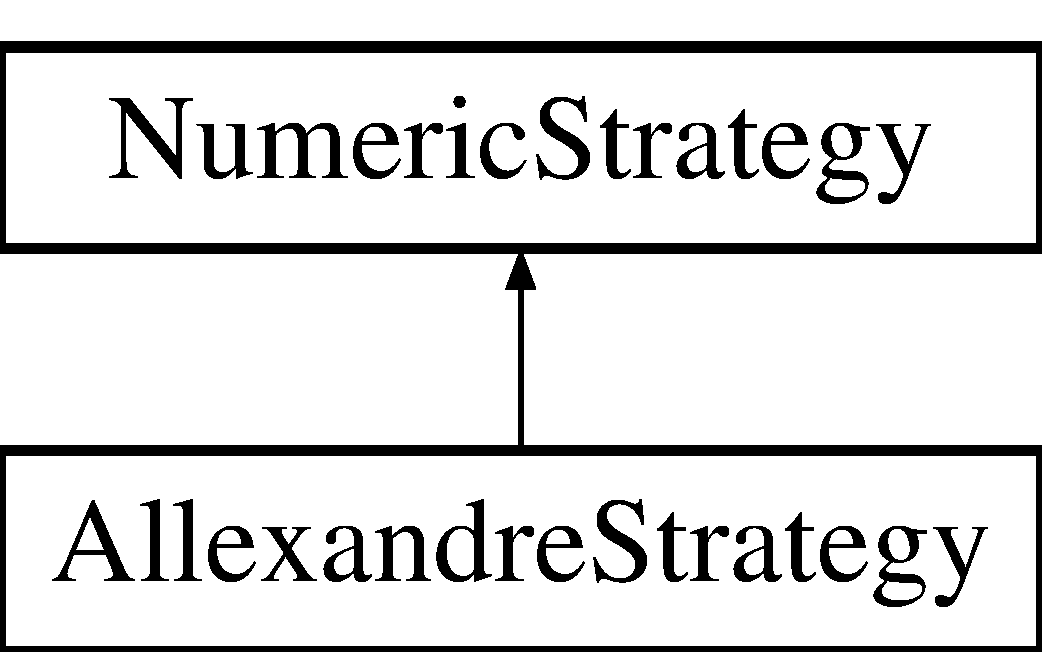
\includegraphics[height=2.000000cm]{class_allexandre_strategy}
\end{center}
\end{figure}
\subsection*{Public Member Functions}
\begin{DoxyCompactItemize}
\item 
\hyperlink{class_allexandre_strategy_ac14cc10857d943bd555f828fd3c8004d}{Allexandre\+Strategy} (\hyperlink{class_cardiac_mesh}{Cardiac\+Mesh} $\ast$oscillators)
\item 
\hyperlink{class_allexandre_strategy_ac8783c05bbc6e3fea1a99b6ff657fb0d}{$\sim$\+Allexandre\+Strategy} ()
\item 
double \hyperlink{class_allexandre_strategy_a25fe69b84aed988807d10e4b72890d26}{step\+Modified\+Backward\+Euler} (\hyperlink{class_oscillator}{Oscillator} $\ast$osc)
\item 
double \hyperlink{class_allexandre_strategy_a418e280a746b6105eb609cbee6ea99fc}{next\+Step} ()
\begin{DoxyCompactList}\small\item\em Main function. \end{DoxyCompactList}\item 
void \hyperlink{class_allexandre_strategy_a8f657c6d14d76cef3a312fc862c400f7}{reset} ()
\item 
void \hyperlink{class_allexandre_strategy_a19227368bd05ee1d3df2f655387a2dda}{construct\+Update\+Time\+Tree} ()
\item 
void \hyperlink{class_allexandre_strategy_a194aa637bdd931c1f0541cc11e450c79}{construct\+Timestep\+Tree} ()
\item 
double \hyperlink{class_allexandre_strategy_a9ae2720bb39eeb2044a9192a64e0fa95}{guard\+Cell\+Update} ()
\item 
double \hyperlink{class_allexandre_strategy_aae541b33a9b2183437624ba5ecc083a8}{get\+Delta\+Timestep\+Inc} (double \&v\+\_\+prim)
\item 
double \hyperlink{class_allexandre_strategy_adbcde09e77b6c3091fc972ca135d05d4}{get\+Max\+Timestep\+\_\+\+Method2b} (const double \&v\+\_\+prim, const double \&fast\+\_\+prim, const double \&Kd)
\end{DoxyCompactItemize}
\subsection*{Additional Inherited Members}


\subsection{Constructor \& Destructor Documentation}
\hypertarget{class_allexandre_strategy_ac14cc10857d943bd555f828fd3c8004d}{\index{Allexandre\+Strategy@{Allexandre\+Strategy}!Allexandre\+Strategy@{Allexandre\+Strategy}}
\index{Allexandre\+Strategy@{Allexandre\+Strategy}!Allexandre\+Strategy@{Allexandre\+Strategy}}
\subsubsection[{Allexandre\+Strategy}]{\setlength{\rightskip}{0pt plus 5cm}Allexandre\+Strategy\+::\+Allexandre\+Strategy (
\begin{DoxyParamCaption}
\item[{{\bf Cardiac\+Mesh} $\ast$}]{oscillators}
\end{DoxyParamCaption}
)}}\label{class_allexandre_strategy_ac14cc10857d943bd555f828fd3c8004d}
\hypertarget{class_allexandre_strategy_ac8783c05bbc6e3fea1a99b6ff657fb0d}{\index{Allexandre\+Strategy@{Allexandre\+Strategy}!````~Allexandre\+Strategy@{$\sim$\+Allexandre\+Strategy}}
\index{````~Allexandre\+Strategy@{$\sim$\+Allexandre\+Strategy}!Allexandre\+Strategy@{Allexandre\+Strategy}}
\subsubsection[{$\sim$\+Allexandre\+Strategy}]{\setlength{\rightskip}{0pt plus 5cm}Allexandre\+Strategy\+::$\sim$\+Allexandre\+Strategy (
\begin{DoxyParamCaption}
{}
\end{DoxyParamCaption}
)}}\label{class_allexandre_strategy_ac8783c05bbc6e3fea1a99b6ff657fb0d}


\subsection{Member Function Documentation}
\hypertarget{class_allexandre_strategy_a194aa637bdd931c1f0541cc11e450c79}{\index{Allexandre\+Strategy@{Allexandre\+Strategy}!construct\+Timestep\+Tree@{construct\+Timestep\+Tree}}
\index{construct\+Timestep\+Tree@{construct\+Timestep\+Tree}!Allexandre\+Strategy@{Allexandre\+Strategy}}
\subsubsection[{construct\+Timestep\+Tree}]{\setlength{\rightskip}{0pt plus 5cm}void Allexandre\+Strategy\+::construct\+Timestep\+Tree (
\begin{DoxyParamCaption}
{}
\end{DoxyParamCaption}
)}}\label{class_allexandre_strategy_a194aa637bdd931c1f0541cc11e450c79}
\hypertarget{class_allexandre_strategy_a19227368bd05ee1d3df2f655387a2dda}{\index{Allexandre\+Strategy@{Allexandre\+Strategy}!construct\+Update\+Time\+Tree@{construct\+Update\+Time\+Tree}}
\index{construct\+Update\+Time\+Tree@{construct\+Update\+Time\+Tree}!Allexandre\+Strategy@{Allexandre\+Strategy}}
\subsubsection[{construct\+Update\+Time\+Tree}]{\setlength{\rightskip}{0pt plus 5cm}void Allexandre\+Strategy\+::construct\+Update\+Time\+Tree (
\begin{DoxyParamCaption}
{}
\end{DoxyParamCaption}
)}}\label{class_allexandre_strategy_a19227368bd05ee1d3df2f655387a2dda}
\hypertarget{class_allexandre_strategy_aae541b33a9b2183437624ba5ecc083a8}{\index{Allexandre\+Strategy@{Allexandre\+Strategy}!get\+Delta\+Timestep\+Inc@{get\+Delta\+Timestep\+Inc}}
\index{get\+Delta\+Timestep\+Inc@{get\+Delta\+Timestep\+Inc}!Allexandre\+Strategy@{Allexandre\+Strategy}}
\subsubsection[{get\+Delta\+Timestep\+Inc}]{\setlength{\rightskip}{0pt plus 5cm}double Allexandre\+Strategy\+::get\+Delta\+Timestep\+Inc (
\begin{DoxyParamCaption}
\item[{double \&}]{v\+\_\+prim}
\end{DoxyParamCaption}
)}}\label{class_allexandre_strategy_aae541b33a9b2183437624ba5ecc083a8}
\hypertarget{class_allexandre_strategy_adbcde09e77b6c3091fc972ca135d05d4}{\index{Allexandre\+Strategy@{Allexandre\+Strategy}!get\+Max\+Timestep\+\_\+\+Method2b@{get\+Max\+Timestep\+\_\+\+Method2b}}
\index{get\+Max\+Timestep\+\_\+\+Method2b@{get\+Max\+Timestep\+\_\+\+Method2b}!Allexandre\+Strategy@{Allexandre\+Strategy}}
\subsubsection[{get\+Max\+Timestep\+\_\+\+Method2b}]{\setlength{\rightskip}{0pt plus 5cm}double Allexandre\+Strategy\+::get\+Max\+Timestep\+\_\+\+Method2b (
\begin{DoxyParamCaption}
\item[{const double \&}]{v\+\_\+prim, }
\item[{const double \&}]{fast\+\_\+prim, }
\item[{const double \&}]{Kd}
\end{DoxyParamCaption}
)}}\label{class_allexandre_strategy_adbcde09e77b6c3091fc972ca135d05d4}
\hypertarget{class_allexandre_strategy_a9ae2720bb39eeb2044a9192a64e0fa95}{\index{Allexandre\+Strategy@{Allexandre\+Strategy}!guard\+Cell\+Update@{guard\+Cell\+Update}}
\index{guard\+Cell\+Update@{guard\+Cell\+Update}!Allexandre\+Strategy@{Allexandre\+Strategy}}
\subsubsection[{guard\+Cell\+Update}]{\setlength{\rightskip}{0pt plus 5cm}double Allexandre\+Strategy\+::guard\+Cell\+Update (
\begin{DoxyParamCaption}
{}
\end{DoxyParamCaption}
)}}\label{class_allexandre_strategy_a9ae2720bb39eeb2044a9192a64e0fa95}
\hypertarget{class_allexandre_strategy_a418e280a746b6105eb609cbee6ea99fc}{\index{Allexandre\+Strategy@{Allexandre\+Strategy}!next\+Step@{next\+Step}}
\index{next\+Step@{next\+Step}!Allexandre\+Strategy@{Allexandre\+Strategy}}
\subsubsection[{next\+Step}]{\setlength{\rightskip}{0pt plus 5cm}double Allexandre\+Strategy\+::next\+Step (
\begin{DoxyParamCaption}
{}
\end{DoxyParamCaption}
)\hspace{0.3cm}{\ttfamily [virtual]}}}\label{class_allexandre_strategy_a418e280a746b6105eb609cbee6ea99fc}


Main function. 



Implements \hyperlink{class_numeric_strategy_aeab387274e9d0ebf46a0e5ad5a5fe73f}{Numeric\+Strategy}.

\hypertarget{class_allexandre_strategy_a8f657c6d14d76cef3a312fc862c400f7}{\index{Allexandre\+Strategy@{Allexandre\+Strategy}!reset@{reset}}
\index{reset@{reset}!Allexandre\+Strategy@{Allexandre\+Strategy}}
\subsubsection[{reset}]{\setlength{\rightskip}{0pt plus 5cm}void Allexandre\+Strategy\+::reset (
\begin{DoxyParamCaption}
{}
\end{DoxyParamCaption}
)}}\label{class_allexandre_strategy_a8f657c6d14d76cef3a312fc862c400f7}
\hypertarget{class_allexandre_strategy_a25fe69b84aed988807d10e4b72890d26}{\index{Allexandre\+Strategy@{Allexandre\+Strategy}!step\+Modified\+Backward\+Euler@{step\+Modified\+Backward\+Euler}}
\index{step\+Modified\+Backward\+Euler@{step\+Modified\+Backward\+Euler}!Allexandre\+Strategy@{Allexandre\+Strategy}}
\subsubsection[{step\+Modified\+Backward\+Euler}]{\setlength{\rightskip}{0pt plus 5cm}double Allexandre\+Strategy\+::step\+Modified\+Backward\+Euler (
\begin{DoxyParamCaption}
\item[{{\bf Oscillator} $\ast$}]{osc}
\end{DoxyParamCaption}
)}}\label{class_allexandre_strategy_a25fe69b84aed988807d10e4b72890d26}


The documentation for this class was generated from the following files\+:\begin{DoxyCompactItemize}
\item 
Numeric\+Strategy/\hyperlink{_allexandre_strategy_8h}{Allexandre\+Strategy.\+h}\item 
Numeric\+Strategy/\hyperlink{_allexandre_strategy_8cpp}{Allexandre\+Strategy.\+cpp}\end{DoxyCompactItemize}

\hypertarget{class_atrial_machine2d}{\section{Atrial\+Machine2d Class Reference}
\label{class_atrial_machine2d}\index{Atrial\+Machine2d@{Atrial\+Machine2d}}
}


{\ttfamily \#include $<$Atrial\+Machine2d.\+h$>$}

Inheritance diagram for Atrial\+Machine2d\+:\begin{figure}[H]
\begin{center}
\leavevmode
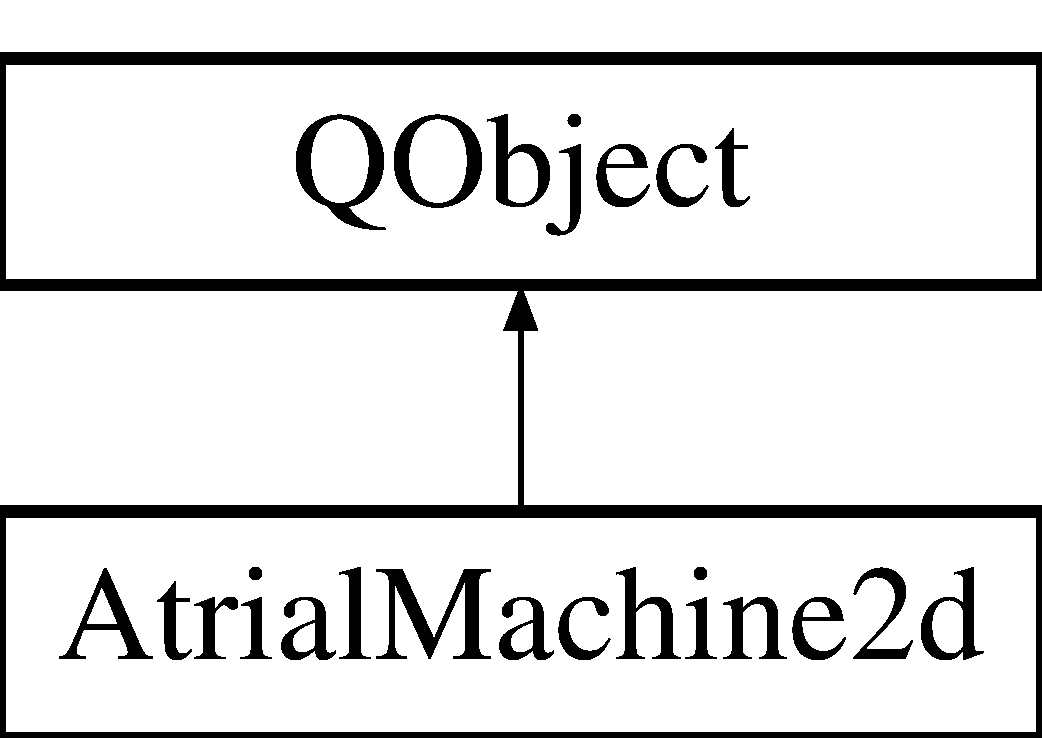
\includegraphics[height=2.000000cm]{class_atrial_machine2d}
\end{center}
\end{figure}
\subsection*{Public Slots}
\begin{DoxyCompactItemize}
\item 
void \hyperlink{class_atrial_machine2d_ab4833c86a56f23867915d876fac581e0}{set\+Forward\+Euler\+Strategy} ()
\item 
void \hyperlink{class_atrial_machine2d_af808c57f5af0c0c26aadcf4c812cb21f}{set\+Allexandre\+Strategy} ()
\item 
double \hyperlink{class_atrial_machine2d_a2a59d6433bd614ff51bc07227210b2e8}{process\+Step} ()
\item 
void \hyperlink{class_atrial_machine2d_a3c509a3d7d9da2b758caa7347bb3ea78}{reset} ()
\item 
void \hyperlink{class_atrial_machine2d_afe82e33fbf54bfc0e75fde82668fba17}{stimulator\+On} ()
\item 
void \hyperlink{class_atrial_machine2d_a4507c491b92b5be2bb8c9493cc67e5cb}{stimulator\+Off} ()
\item 
void \hyperlink{class_atrial_machine2d_a9a600c1251eae56fe59c4188f1735a0b}{calculate\+Full\+Electrogram\+Map} ()
\item 
void \hyperlink{class_atrial_machine2d_a5e5d865f2142795acca445437cc2346d}{set\+Skip} (int skip)
\item 
void \hyperlink{class_atrial_machine2d_a2bc748b9fda32f5efe515474df2c85e6}{set\+Uniform\+Diffusion} (double value)
\item 
void \hyperlink{class_atrial_machine2d_af78de39e9b9eee079240900b932fa5f0}{set\+Uniform\+E\+R\+P} (double value)
\end{DoxyCompactItemize}
\subsection*{Signals}
\begin{DoxyCompactItemize}
\item 
void \hyperlink{class_atrial_machine2d_aa0503c0b65de1d0a3353fa60001b7c7b}{step\+Finished} ()
\end{DoxyCompactItemize}
\subsection*{Public Member Functions}
\begin{DoxyCompactItemize}
\item 
\hyperlink{class_atrial_machine2d_a1181b8a58b70e0374cfaefcbf2c29b12}{Atrial\+Machine2d} (\hyperlink{classatrial_parameters}{atrial\+Parameters} $\ast$definitions, \hyperlink{class_cardiac_mesh}{Cardiac\+Mesh} $\ast$grid)
\item 
\hyperlink{class_atrial_machine2d_a955b6614307d86c8d9e196a3b7ce2434}{$\sim$\+Atrial\+Machine2d} (void)
\item 
void \hyperlink{class_atrial_machine2d_a40366613671e5856d0c3cd0572398dc1}{delete\+Atrium} ()
\item 
void \hyperlink{class_atrial_machine2d_a22a0e5a3d07859721cce24ed253932ed}{init} ()
\end{DoxyCompactItemize}
\subsection*{Public Attributes}
\begin{DoxyCompactItemize}
\item 
void(Atrial\+Machine2d\+::$\ast$ \hyperlink{class_atrial_machine2d_aaeb0690b1fbd433bd0c25f2162b7b4bb}{set\+Strategy} )()
\item 
\hyperlink{classatrial_parameters}{atrial\+Parameters} $\ast$ \hyperlink{class_atrial_machine2d_aeafb998f5621fb19749014161d7d600d}{m\+\_\+definitions}
\item 
\hyperlink{class_random_generator}{Random\+Generator} \hyperlink{class_atrial_machine2d_a4ee41f8430aca76d5c6411cd37c92d38}{generator}
\item 
std\+::vector$<$ \hyperlink{class_probe_electrode}{Probe\+Electrode} $\ast$ $>$ \hyperlink{class_atrial_machine2d_a524fc9fd5d07a9f6f93611ee7839c99c}{probe\+Oscillator}
\item 
\hyperlink{class_cardiac_mesh}{Cardiac\+Mesh} $\ast$ \hyperlink{class_atrial_machine2d_ae5a4568a32980b04648791e7ac5e3249}{m\+\_\+grid}
\item 
\hyperlink{class_numeric_strategy}{Numeric\+Strategy} $\ast$ \hyperlink{class_atrial_machine2d_afa218ce1cafcf45895c0317953b97977}{m\+\_\+strategy}
\item 
\hyperlink{class_ep_stimulator}{Ep\+Stimulator} \hyperlink{class_atrial_machine2d_a932f19f3964c0bf8831fa4fc06a85ab6}{stimulator}
\item 
double \hyperlink{class_atrial_machine2d_a951f2f5f1bee9505ee93df61121bf5d2}{m\+\_\+global\+Time}
\end{DoxyCompactItemize}


\subsection{Constructor \& Destructor Documentation}
\hypertarget{class_atrial_machine2d_a1181b8a58b70e0374cfaefcbf2c29b12}{\index{Atrial\+Machine2d@{Atrial\+Machine2d}!Atrial\+Machine2d@{Atrial\+Machine2d}}
\index{Atrial\+Machine2d@{Atrial\+Machine2d}!Atrial\+Machine2d@{Atrial\+Machine2d}}
\subsubsection[{Atrial\+Machine2d}]{\setlength{\rightskip}{0pt plus 5cm}Atrial\+Machine2d\+::\+Atrial\+Machine2d (
\begin{DoxyParamCaption}
\item[{{\bf atrial\+Parameters} $\ast$}]{definitions, }
\item[{{\bf Cardiac\+Mesh} $\ast$}]{grid}
\end{DoxyParamCaption}
)}}\label{class_atrial_machine2d_a1181b8a58b70e0374cfaefcbf2c29b12}
\hypertarget{class_atrial_machine2d_a955b6614307d86c8d9e196a3b7ce2434}{\index{Atrial\+Machine2d@{Atrial\+Machine2d}!````~Atrial\+Machine2d@{$\sim$\+Atrial\+Machine2d}}
\index{````~Atrial\+Machine2d@{$\sim$\+Atrial\+Machine2d}!Atrial\+Machine2d@{Atrial\+Machine2d}}
\subsubsection[{$\sim$\+Atrial\+Machine2d}]{\setlength{\rightskip}{0pt plus 5cm}Atrial\+Machine2d\+::$\sim$\+Atrial\+Machine2d (
\begin{DoxyParamCaption}
\item[{void}]{}
\end{DoxyParamCaption}
)}}\label{class_atrial_machine2d_a955b6614307d86c8d9e196a3b7ce2434}


\subsection{Member Function Documentation}
\hypertarget{class_atrial_machine2d_a9a600c1251eae56fe59c4188f1735a0b}{\index{Atrial\+Machine2d@{Atrial\+Machine2d}!calculate\+Full\+Electrogram\+Map@{calculate\+Full\+Electrogram\+Map}}
\index{calculate\+Full\+Electrogram\+Map@{calculate\+Full\+Electrogram\+Map}!Atrial\+Machine2d@{Atrial\+Machine2d}}
\subsubsection[{calculate\+Full\+Electrogram\+Map}]{\setlength{\rightskip}{0pt plus 5cm}void Atrial\+Machine2d\+::calculate\+Full\+Electrogram\+Map (
\begin{DoxyParamCaption}
{}
\end{DoxyParamCaption}
)\hspace{0.3cm}{\ttfamily [slot]}}}\label{class_atrial_machine2d_a9a600c1251eae56fe59c4188f1735a0b}
\hypertarget{class_atrial_machine2d_a40366613671e5856d0c3cd0572398dc1}{\index{Atrial\+Machine2d@{Atrial\+Machine2d}!delete\+Atrium@{delete\+Atrium}}
\index{delete\+Atrium@{delete\+Atrium}!Atrial\+Machine2d@{Atrial\+Machine2d}}
\subsubsection[{delete\+Atrium}]{\setlength{\rightskip}{0pt plus 5cm}void Atrial\+Machine2d\+::delete\+Atrium (
\begin{DoxyParamCaption}
{}
\end{DoxyParamCaption}
)}}\label{class_atrial_machine2d_a40366613671e5856d0c3cd0572398dc1}
\hypertarget{class_atrial_machine2d_a22a0e5a3d07859721cce24ed253932ed}{\index{Atrial\+Machine2d@{Atrial\+Machine2d}!init@{init}}
\index{init@{init}!Atrial\+Machine2d@{Atrial\+Machine2d}}
\subsubsection[{init}]{\setlength{\rightskip}{0pt plus 5cm}void Atrial\+Machine2d\+::init (
\begin{DoxyParamCaption}
{}
\end{DoxyParamCaption}
)}}\label{class_atrial_machine2d_a22a0e5a3d07859721cce24ed253932ed}
\hypertarget{class_atrial_machine2d_a2a59d6433bd614ff51bc07227210b2e8}{\index{Atrial\+Machine2d@{Atrial\+Machine2d}!process\+Step@{process\+Step}}
\index{process\+Step@{process\+Step}!Atrial\+Machine2d@{Atrial\+Machine2d}}
\subsubsection[{process\+Step}]{\setlength{\rightskip}{0pt plus 5cm}double Atrial\+Machine2d\+::process\+Step (
\begin{DoxyParamCaption}
{}
\end{DoxyParamCaption}
)\hspace{0.3cm}{\ttfamily [slot]}}}\label{class_atrial_machine2d_a2a59d6433bd614ff51bc07227210b2e8}
\hypertarget{class_atrial_machine2d_a3c509a3d7d9da2b758caa7347bb3ea78}{\index{Atrial\+Machine2d@{Atrial\+Machine2d}!reset@{reset}}
\index{reset@{reset}!Atrial\+Machine2d@{Atrial\+Machine2d}}
\subsubsection[{reset}]{\setlength{\rightskip}{0pt plus 5cm}void Atrial\+Machine2d\+::reset (
\begin{DoxyParamCaption}
{}
\end{DoxyParamCaption}
)\hspace{0.3cm}{\ttfamily [slot]}}}\label{class_atrial_machine2d_a3c509a3d7d9da2b758caa7347bb3ea78}
\hypertarget{class_atrial_machine2d_af808c57f5af0c0c26aadcf4c812cb21f}{\index{Atrial\+Machine2d@{Atrial\+Machine2d}!set\+Allexandre\+Strategy@{set\+Allexandre\+Strategy}}
\index{set\+Allexandre\+Strategy@{set\+Allexandre\+Strategy}!Atrial\+Machine2d@{Atrial\+Machine2d}}
\subsubsection[{set\+Allexandre\+Strategy}]{\setlength{\rightskip}{0pt plus 5cm}void Atrial\+Machine2d\+::set\+Allexandre\+Strategy (
\begin{DoxyParamCaption}
{}
\end{DoxyParamCaption}
)\hspace{0.3cm}{\ttfamily [slot]}}}\label{class_atrial_machine2d_af808c57f5af0c0c26aadcf4c812cb21f}
\hypertarget{class_atrial_machine2d_ab4833c86a56f23867915d876fac581e0}{\index{Atrial\+Machine2d@{Atrial\+Machine2d}!set\+Forward\+Euler\+Strategy@{set\+Forward\+Euler\+Strategy}}
\index{set\+Forward\+Euler\+Strategy@{set\+Forward\+Euler\+Strategy}!Atrial\+Machine2d@{Atrial\+Machine2d}}
\subsubsection[{set\+Forward\+Euler\+Strategy}]{\setlength{\rightskip}{0pt plus 5cm}void Atrial\+Machine2d\+::set\+Forward\+Euler\+Strategy (
\begin{DoxyParamCaption}
{}
\end{DoxyParamCaption}
)\hspace{0.3cm}{\ttfamily [slot]}}}\label{class_atrial_machine2d_ab4833c86a56f23867915d876fac581e0}
\hypertarget{class_atrial_machine2d_a5e5d865f2142795acca445437cc2346d}{\index{Atrial\+Machine2d@{Atrial\+Machine2d}!set\+Skip@{set\+Skip}}
\index{set\+Skip@{set\+Skip}!Atrial\+Machine2d@{Atrial\+Machine2d}}
\subsubsection[{set\+Skip}]{\setlength{\rightskip}{0pt plus 5cm}void Atrial\+Machine2d\+::set\+Skip (
\begin{DoxyParamCaption}
\item[{int}]{skip}
\end{DoxyParamCaption}
)\hspace{0.3cm}{\ttfamily [slot]}}}\label{class_atrial_machine2d_a5e5d865f2142795acca445437cc2346d}
\hypertarget{class_atrial_machine2d_a2bc748b9fda32f5efe515474df2c85e6}{\index{Atrial\+Machine2d@{Atrial\+Machine2d}!set\+Uniform\+Diffusion@{set\+Uniform\+Diffusion}}
\index{set\+Uniform\+Diffusion@{set\+Uniform\+Diffusion}!Atrial\+Machine2d@{Atrial\+Machine2d}}
\subsubsection[{set\+Uniform\+Diffusion}]{\setlength{\rightskip}{0pt plus 5cm}void Atrial\+Machine2d\+::set\+Uniform\+Diffusion (
\begin{DoxyParamCaption}
\item[{double}]{value}
\end{DoxyParamCaption}
)\hspace{0.3cm}{\ttfamily [slot]}}}\label{class_atrial_machine2d_a2bc748b9fda32f5efe515474df2c85e6}
\hypertarget{class_atrial_machine2d_af78de39e9b9eee079240900b932fa5f0}{\index{Atrial\+Machine2d@{Atrial\+Machine2d}!set\+Uniform\+E\+R\+P@{set\+Uniform\+E\+R\+P}}
\index{set\+Uniform\+E\+R\+P@{set\+Uniform\+E\+R\+P}!Atrial\+Machine2d@{Atrial\+Machine2d}}
\subsubsection[{set\+Uniform\+E\+R\+P}]{\setlength{\rightskip}{0pt plus 5cm}void Atrial\+Machine2d\+::set\+Uniform\+E\+R\+P (
\begin{DoxyParamCaption}
\item[{double}]{value}
\end{DoxyParamCaption}
)\hspace{0.3cm}{\ttfamily [slot]}}}\label{class_atrial_machine2d_af78de39e9b9eee079240900b932fa5f0}
\hypertarget{class_atrial_machine2d_aa0503c0b65de1d0a3353fa60001b7c7b}{\index{Atrial\+Machine2d@{Atrial\+Machine2d}!step\+Finished@{step\+Finished}}
\index{step\+Finished@{step\+Finished}!Atrial\+Machine2d@{Atrial\+Machine2d}}
\subsubsection[{step\+Finished}]{\setlength{\rightskip}{0pt plus 5cm}void Atrial\+Machine2d\+::step\+Finished (
\begin{DoxyParamCaption}
{}
\end{DoxyParamCaption}
)\hspace{0.3cm}{\ttfamily [signal]}}}\label{class_atrial_machine2d_aa0503c0b65de1d0a3353fa60001b7c7b}
\hypertarget{class_atrial_machine2d_a4507c491b92b5be2bb8c9493cc67e5cb}{\index{Atrial\+Machine2d@{Atrial\+Machine2d}!stimulator\+Off@{stimulator\+Off}}
\index{stimulator\+Off@{stimulator\+Off}!Atrial\+Machine2d@{Atrial\+Machine2d}}
\subsubsection[{stimulator\+Off}]{\setlength{\rightskip}{0pt plus 5cm}void Atrial\+Machine2d\+::stimulator\+Off (
\begin{DoxyParamCaption}
{}
\end{DoxyParamCaption}
)\hspace{0.3cm}{\ttfamily [slot]}}}\label{class_atrial_machine2d_a4507c491b92b5be2bb8c9493cc67e5cb}
\hypertarget{class_atrial_machine2d_afe82e33fbf54bfc0e75fde82668fba17}{\index{Atrial\+Machine2d@{Atrial\+Machine2d}!stimulator\+On@{stimulator\+On}}
\index{stimulator\+On@{stimulator\+On}!Atrial\+Machine2d@{Atrial\+Machine2d}}
\subsubsection[{stimulator\+On}]{\setlength{\rightskip}{0pt plus 5cm}void Atrial\+Machine2d\+::stimulator\+On (
\begin{DoxyParamCaption}
{}
\end{DoxyParamCaption}
)\hspace{0.3cm}{\ttfamily [slot]}}}\label{class_atrial_machine2d_afe82e33fbf54bfc0e75fde82668fba17}


\subsection{Member Data Documentation}
\hypertarget{class_atrial_machine2d_a4ee41f8430aca76d5c6411cd37c92d38}{\index{Atrial\+Machine2d@{Atrial\+Machine2d}!generator@{generator}}
\index{generator@{generator}!Atrial\+Machine2d@{Atrial\+Machine2d}}
\subsubsection[{generator}]{\setlength{\rightskip}{0pt plus 5cm}{\bf Random\+Generator} Atrial\+Machine2d\+::generator}}\label{class_atrial_machine2d_a4ee41f8430aca76d5c6411cd37c92d38}
\hypertarget{class_atrial_machine2d_aeafb998f5621fb19749014161d7d600d}{\index{Atrial\+Machine2d@{Atrial\+Machine2d}!m\+\_\+definitions@{m\+\_\+definitions}}
\index{m\+\_\+definitions@{m\+\_\+definitions}!Atrial\+Machine2d@{Atrial\+Machine2d}}
\subsubsection[{m\+\_\+definitions}]{\setlength{\rightskip}{0pt plus 5cm}{\bf atrial\+Parameters}$\ast$ Atrial\+Machine2d\+::m\+\_\+definitions}}\label{class_atrial_machine2d_aeafb998f5621fb19749014161d7d600d}
\hypertarget{class_atrial_machine2d_a951f2f5f1bee9505ee93df61121bf5d2}{\index{Atrial\+Machine2d@{Atrial\+Machine2d}!m\+\_\+global\+Time@{m\+\_\+global\+Time}}
\index{m\+\_\+global\+Time@{m\+\_\+global\+Time}!Atrial\+Machine2d@{Atrial\+Machine2d}}
\subsubsection[{m\+\_\+global\+Time}]{\setlength{\rightskip}{0pt plus 5cm}double Atrial\+Machine2d\+::m\+\_\+global\+Time}}\label{class_atrial_machine2d_a951f2f5f1bee9505ee93df61121bf5d2}
\hypertarget{class_atrial_machine2d_ae5a4568a32980b04648791e7ac5e3249}{\index{Atrial\+Machine2d@{Atrial\+Machine2d}!m\+\_\+grid@{m\+\_\+grid}}
\index{m\+\_\+grid@{m\+\_\+grid}!Atrial\+Machine2d@{Atrial\+Machine2d}}
\subsubsection[{m\+\_\+grid}]{\setlength{\rightskip}{0pt plus 5cm}{\bf Cardiac\+Mesh}$\ast$ Atrial\+Machine2d\+::m\+\_\+grid}}\label{class_atrial_machine2d_ae5a4568a32980b04648791e7ac5e3249}
\hypertarget{class_atrial_machine2d_afa218ce1cafcf45895c0317953b97977}{\index{Atrial\+Machine2d@{Atrial\+Machine2d}!m\+\_\+strategy@{m\+\_\+strategy}}
\index{m\+\_\+strategy@{m\+\_\+strategy}!Atrial\+Machine2d@{Atrial\+Machine2d}}
\subsubsection[{m\+\_\+strategy}]{\setlength{\rightskip}{0pt plus 5cm}{\bf Numeric\+Strategy}$\ast$ Atrial\+Machine2d\+::m\+\_\+strategy}}\label{class_atrial_machine2d_afa218ce1cafcf45895c0317953b97977}
\hypertarget{class_atrial_machine2d_a524fc9fd5d07a9f6f93611ee7839c99c}{\index{Atrial\+Machine2d@{Atrial\+Machine2d}!probe\+Oscillator@{probe\+Oscillator}}
\index{probe\+Oscillator@{probe\+Oscillator}!Atrial\+Machine2d@{Atrial\+Machine2d}}
\subsubsection[{probe\+Oscillator}]{\setlength{\rightskip}{0pt plus 5cm}std\+::vector$<${\bf Probe\+Electrode}$\ast$$>$ Atrial\+Machine2d\+::probe\+Oscillator}}\label{class_atrial_machine2d_a524fc9fd5d07a9f6f93611ee7839c99c}
\hypertarget{class_atrial_machine2d_aaeb0690b1fbd433bd0c25f2162b7b4bb}{\index{Atrial\+Machine2d@{Atrial\+Machine2d}!set\+Strategy@{set\+Strategy}}
\index{set\+Strategy@{set\+Strategy}!Atrial\+Machine2d@{Atrial\+Machine2d}}
\subsubsection[{set\+Strategy}]{\setlength{\rightskip}{0pt plus 5cm}void(Atrial\+Machine2d\+::$\ast$ Atrial\+Machine2d\+::set\+Strategy)()}}\label{class_atrial_machine2d_aaeb0690b1fbd433bd0c25f2162b7b4bb}
\hypertarget{class_atrial_machine2d_a932f19f3964c0bf8831fa4fc06a85ab6}{\index{Atrial\+Machine2d@{Atrial\+Machine2d}!stimulator@{stimulator}}
\index{stimulator@{stimulator}!Atrial\+Machine2d@{Atrial\+Machine2d}}
\subsubsection[{stimulator}]{\setlength{\rightskip}{0pt plus 5cm}{\bf Ep\+Stimulator} Atrial\+Machine2d\+::stimulator}}\label{class_atrial_machine2d_a932f19f3964c0bf8831fa4fc06a85ab6}


The documentation for this class was generated from the following files\+:\begin{DoxyCompactItemize}
\item 
\hyperlink{_atrial_machine2d_8h}{Atrial\+Machine2d.\+h}\item 
\hyperlink{_atrial_machine2d_8cpp}{Atrial\+Machine2d.\+cpp}\end{DoxyCompactItemize}

\hypertarget{classatrial_parameters}{\section{atrial\+Parameters Class Reference}
\label{classatrial_parameters}\index{atrial\+Parameters@{atrial\+Parameters}}
}


{\ttfamily \#include $<$atrial\+Parameters.\+h$>$}

Inheritance diagram for atrial\+Parameters\+:\begin{figure}[H]
\begin{center}
\leavevmode
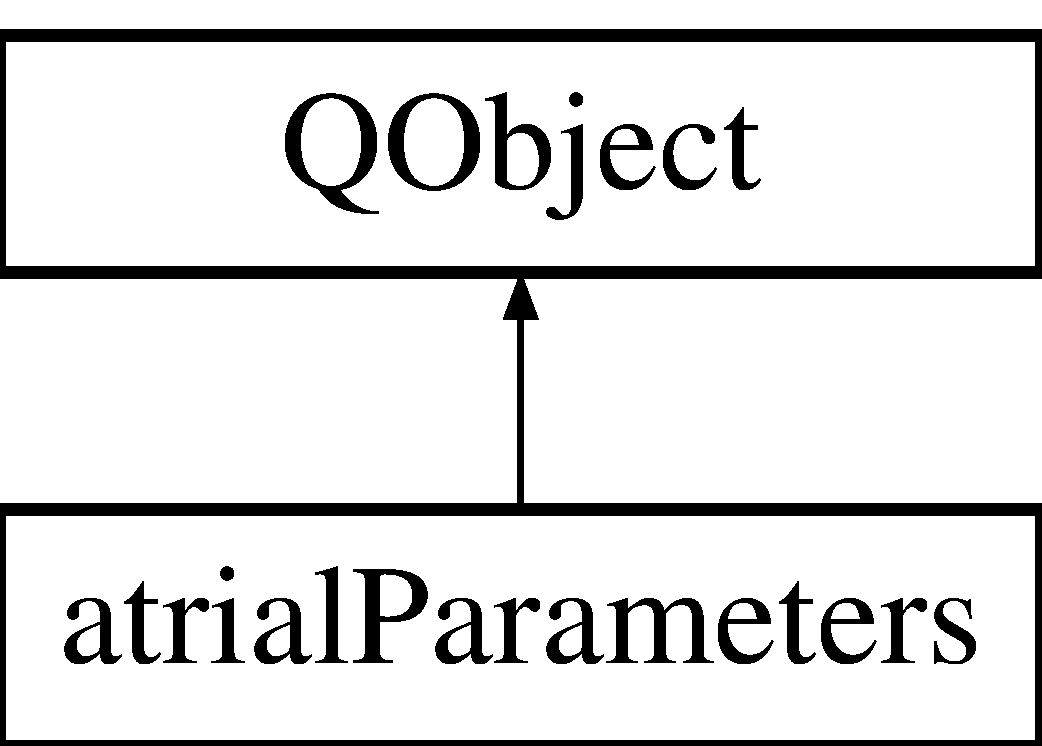
\includegraphics[height=2.000000cm]{classatrial_parameters}
\end{center}
\end{figure}
\subsection*{Public Slots}
\begin{DoxyCompactItemize}
\item 
void \hyperlink{classatrial_parameters_a78d1ea1d1f6c256851cf7b83a8a21707}{set\+Main\+Time\+Step} (double timestep)
\item 
void \hyperlink{classatrial_parameters_a7606b5002a1af27bc97187d2e6c3627b}{set\+Skip} (int skip)
\item 
void \hyperlink{classatrial_parameters_a4dd8c8fb864448c607126b224dc9179f}{set\+Euler} ()
\item 
void \hyperlink{classatrial_parameters_a8debca6529b58fa7105c2cf339c9b94d}{set\+Duffort} ()
\item 
void \hyperlink{classatrial_parameters_ad9e7b355f6c3e0daba1146094fd3ddaa}{set\+Kutta} ()
\item 
void \hyperlink{classatrial_parameters_a4c355267171aa97dda88cf96dd205e92}{set\+Ectopic\+Size} (int value)
\item 
void \hyperlink{classatrial_parameters_a9b0cce5a057acb4b7180b783268f0d1b}{set\+Ectopic\+Amplitude} (double value)
\item 
void \hyperlink{classatrial_parameters_a331034e42e78eee66c208855f1bf871b}{set\+Ectopic\+Period} (double value)
\item 
void \hyperlink{classatrial_parameters_a4d86ff607fd2c7b05256fae26883f076}{set\+Ectopic\+Length} (double value)
\item 
void \hyperlink{classatrial_parameters_a8d9fad90f88588a4fb4f28db435afc7a}{set\+Ectopic\+Pos\+X} (int value)
\item 
void \hyperlink{classatrial_parameters_a0599af0dbe33406d002439d4d217fbd2}{set\+Ectopic\+Pos\+Y} (int value)
\item 
void \hyperlink{classatrial_parameters_a1a3511950c14ba3ba34eae948f18380f}{set\+Ectopic\+Shape} (int value)
\item 
void \hyperlink{classatrial_parameters_a4d79c3892b7b7378e03956a843969a50}{toggle\+Ectopic\+Activity} (bool value)
\item 
void \hyperlink{classatrial_parameters_ac3b7b3af7884c95d00e9bcc4e3a5e232}{toggle\+Ectopic\+Mod\+Activity} (bool value)
\item 
void \hyperlink{classatrial_parameters_abf71a393c2ba83420004f8b247c18632}{set\+Ecto\+Mod\+Time} (double value)
\item 
void \hyperlink{classatrial_parameters_aa8568ffc4c3280b182f1c99a270c2828}{set\+Sa\+Global\+Alpha} (double value)
\item 
void \hyperlink{classatrial_parameters_a2c9c09fe672d04ac68f1356343fad669}{set\+Sa\+Global\+F} (double value)
\item 
void \hyperlink{classatrial_parameters_aee40af07411f17363ea06d6c7b40d3d3}{set\+Sa\+Global\+D} (double value)
\item 
void \hyperlink{classatrial_parameters_af51880cf3645288dddce20513a85899c}{set\+Sa\+Global\+E} (double value)
\item 
void \hyperlink{classatrial_parameters_aa14935f63b78f52f90e684e17af2e8be}{set\+Sa\+Global\+V1} (double value)
\item 
void \hyperlink{classatrial_parameters_afb57088c6955f7faa92a5f55137d661a}{set\+Sa\+Global\+V2} (double value)
\item 
void \hyperlink{classatrial_parameters_ae6ea3d79d98a9a573f69979672b99297}{set\+Sa\+Global\+Time\+Scaler} (double value)
\item 
void \hyperlink{classatrial_parameters_afe41a61763e7956fade78d2add1d6a1f}{set\+Sa\+Global\+Alpha\+\_\+2} (double value)
\item 
void \hyperlink{classatrial_parameters_a37e9a313eac8ad8ac1a3cad56a99ea4b}{set\+Sa\+Global\+F\+\_\+2} (double value)
\item 
void \hyperlink{classatrial_parameters_a90f67e724ae64337fe1347cf8b61db9d}{set\+Sa\+Global\+D\+\_\+2} (double value)
\item 
void \hyperlink{classatrial_parameters_a4996b46ae8f31e1a13c3754fec4ad11b}{set\+Sa\+Global\+E\+\_\+2} (double value)
\item 
void \hyperlink{classatrial_parameters_a7a417159e294c3a2b720e6ce362a23d0}{set\+Sa\+Global\+V1\+\_\+2} (double value)
\item 
void \hyperlink{classatrial_parameters_ace08ad55c3eda49782c6fcd5f897f597}{set\+Sa\+Global\+V2\+\_\+2} (double value)
\item 
void \hyperlink{classatrial_parameters_a4d3d26175f5ba0802d6fc6668fdcd6f7}{set\+Sa\+Global\+Time\+Scaler\+\_\+2} (double value)
\item 
void \hyperlink{classatrial_parameters_a88cb4bf667199e2852f575e99730ea0f}{set\+Av\+Global\+Alpha} (double value)
\item 
void \hyperlink{classatrial_parameters_ae6a6825493988fbacb12e1bd570651ef}{set\+Av\+Global\+F} (double value)
\item 
void \hyperlink{classatrial_parameters_aca462126cc7e8b71fb9c3cf02a24face}{set\+Av\+Global\+D} (double value)
\item 
void \hyperlink{classatrial_parameters_a3a71ae994474119d5b481225b687733c}{set\+Av\+Global\+E} (double value)
\item 
void \hyperlink{classatrial_parameters_a28b1fbc725ef53ec978dbf46db2f9324}{set\+Av\+Global\+V1} (double value)
\item 
void \hyperlink{classatrial_parameters_ae725daa5fc0b643658308a3f21d3d792}{set\+Av\+Global\+V2} (double value)
\item 
void \hyperlink{classatrial_parameters_a9d98fa5d7e0d234cdc2a1011d07be4d7}{set\+Av\+Global\+Time\+Scaler} (double value)
\item 
void \hyperlink{classatrial_parameters_a59022c60d080766027ba858f721566c7}{set\+Atrium\+Global\+Gamma} (double value)
\item 
void \hyperlink{classatrial_parameters_a28e741282c70b4051cbe947da9c73381}{set\+Atrium\+Global\+Beta} (double value)
\item 
void \hyperlink{classatrial_parameters_ac3ab123a68d6818ba5d5a04e091b936d}{set\+Atrium\+Global\+Ni} (double value)
\item 
void \hyperlink{classatrial_parameters_a29786fb5f5b2e5995f064c2d4f71f2f5}{set\+Atrium\+Global\+C1} (double value)
\item 
void \hyperlink{classatrial_parameters_a2531ce977adbc7e06959fb0e8254cced}{set\+Atrium\+Global\+C2} (double value)
\item 
void \hyperlink{classatrial_parameters_a7b26befa3c022befa5eda7408920d379}{set\+Atrium\+Global\+Alpha} (double value)
\item 
void \hyperlink{classatrial_parameters_ac0c7bbe4dcbf683207f9002b47729853}{set\+Atrium\+Global\+Time\+Scaler} (double value)
\item 
void \hyperlink{classatrial_parameters_a6ebc25960fcf64eedf8c8cfc69b50f72}{set\+Av\+Global\+Alpha\+\_\+2} (double value)
\item 
void \hyperlink{classatrial_parameters_a82bf0b71848b0702e1b82045809939ac}{set\+Av\+Global\+F\+\_\+2} (double value)
\item 
void \hyperlink{classatrial_parameters_a8c4335fa40ad96dd29f37c08b8ed5765}{set\+Av\+Global\+D\+\_\+2} (double value)
\item 
void \hyperlink{classatrial_parameters_a2fcbd84425603c3dbe27fdaee99c8991}{set\+Av\+Global\+E\+\_\+2} (double value)
\item 
void \hyperlink{classatrial_parameters_a4d325be618a9fa4b0a42976d602b1560}{set\+Av\+Global\+V1\+\_\+2} (double value)
\item 
void \hyperlink{classatrial_parameters_a93d13234748730c7850cf36525a40b71}{set\+Av\+Global\+V2\+\_\+2} (double value)
\item 
void \hyperlink{classatrial_parameters_a510dcbc3ee2997b618474595176ae1bf}{set\+Av\+Global\+Time\+Scaler\+\_\+2} (double value)
\item 
void \hyperlink{classatrial_parameters_a5a42c07d852c4d034798acad60b4bc90}{set\+Atrium\+Global\+Gamma\+\_\+2} (double value)
\item 
void \hyperlink{classatrial_parameters_a565dcda6238511b7ac426bebc6efc591}{set\+Atrium\+Global\+Beta\+\_\+2} (double value)
\item 
void \hyperlink{classatrial_parameters_ad6b7ed91bba174fc0384aa779af0b217}{set\+Atrium\+Global\+Ni\+\_\+2} (double value)
\item 
void \hyperlink{classatrial_parameters_a6787a409b2f58c0b3404d9ad92183497}{set\+Atrium\+Global\+C1\+\_\+2} (double value)
\item 
void \hyperlink{classatrial_parameters_adbdea229fc948ee9b66c7e374ada2c07}{set\+Atrium\+Global\+C2\+\_\+2} (double value)
\item 
void \hyperlink{classatrial_parameters_a499526e46d0c55c95f1e15a5bd08a69e}{set\+Atrium\+Global\+Alpha\+\_\+2} (double value)
\item 
void \hyperlink{classatrial_parameters_ac4f6b96428e4f1db6f09a54963728eb2}{set\+Atrium\+Global\+Time\+Scaler\+\_\+2} (double value)
\item 
void \hyperlink{classatrial_parameters_a950313f8a0a6bcb0d818cee5a26f3477}{set\+Save\+R\+R} (bool value)
\item 
void \hyperlink{classatrial_parameters_ab299e636262065b0423eff7ed72bc263}{set\+Ssave\+Potential\+Plots} (bool value)
\item 
void \hyperlink{classatrial_parameters_a8b026a6bf17e0db843e270df17402b80}{set\+Save\+Phase\+Plots} (bool value)
\item 
void \hyperlink{classatrial_parameters_a82ea1217c9a9aff9708b60f267404f43}{set\+Save\+Pictures} (bool value)
\item 
void \hyperlink{classatrial_parameters_ae949242a4bd383e3c311f7def975d98b}{set\+Pictures\+Delay} (int value)
\item 
void \hyperlink{classatrial_parameters_abd17e877da4177a50b378111355f3c46}{set\+Electrode1\+\_\+position\+X} (int value)
\item 
void \hyperlink{classatrial_parameters_ad2ff037410e50382409c0993e09d9ae4}{set\+Electrode1\+\_\+position\+Y} (int value)
\item 
void \hyperlink{classatrial_parameters_ad2ecccd64402e3f9f9f197d969ff58e9}{set\+Electrode2\+\_\+position\+X} (int value)
\item 
void \hyperlink{classatrial_parameters_a66798a95755bbe346a9246ddb7e1d02b}{set\+Electrode2\+\_\+position\+Y} (int value)
\item 
void \hyperlink{classatrial_parameters_a2336c830af73068117a93804c5c694e4}{set\+Electrode3\+\_\+position\+X} (int value)
\item 
void \hyperlink{classatrial_parameters_a04207d9997beba0537867757d6423e85}{set\+Electrode3\+\_\+position\+Y} (int value)
\item 
void \hyperlink{classatrial_parameters_a6c9455e7633f4d4c52e0533057de0690}{set\+Bin\+Size} (double value)
\item 
void \hyperlink{classatrial_parameters_a450421c3abc5eecff0bca9f73a7a72d8}{set\+Tau} (int value)
\item 
void \hyperlink{classatrial_parameters_a70d48a5b6678542337abedc02954c29d}{set\+Window\+Size} (int value)
\end{DoxyCompactItemize}
\subsection*{Public Member Functions}
\begin{DoxyCompactItemize}
\item 
\hyperlink{classatrial_parameters_ab1f58bc297661ea9d029ea59c4d7b59f}{atrial\+Parameters} (void)
\item 
\hyperlink{classatrial_parameters_aa930d083682b226f2341beb27a593a4a}{$\sim$atrial\+Parameters} (void)
\end{DoxyCompactItemize}
\subsection*{Public Attributes}
\begin{DoxyCompactItemize}
\item 
double \hyperlink{classatrial_parameters_a0fc87681256f95d4354e128ff5cacf84}{m\+\_\+main\+Timestep}
\item 
int \hyperlink{classatrial_parameters_a8ff21c69a731af1992ad8f5f39deec96}{m\+\_\+main\+Skip}
\item 
\hyperlink{heart_defines_8h_ae0e356ca8deebb30aca0cd91e0cbd46c}{S\+W\+\_\+\+A\+L\+G\+O\+R\+I\+T\+H\+M\+S} \hyperlink{classatrial_parameters_af7a2c1518dfbdaaec6c3dd4d6d0883d9}{m\+\_\+algorithm\+Type}
\item 
double \hyperlink{classatrial_parameters_ac820bd58444854634cc58275037125e8}{m\+\_\+ecto\+Mod\+Time}
\item 
bool \hyperlink{classatrial_parameters_a9e4bac6934ba9adb8b1316df2ec56511}{m\+\_\+ectopic\+S1\+\_\+toggle}
\item 
bool \hyperlink{classatrial_parameters_a6abb9ccfeef719f0bcb6e69b92c76404}{m\+\_\+ectopic\+S2\+\_\+toggle}
\item 
bool \hyperlink{classatrial_parameters_a9fa3baf0ea436a1f91e8569c9c35b083}{m\+\_\+ectopic\+Activity}
\item 
double \hyperlink{classatrial_parameters_a734cc1920e198bb8eca851f7e8e1433b}{m\+\_\+ectopic\+Amplitude}
\item 
double \hyperlink{classatrial_parameters_a99ef346837d7a634a65fb2d78da439e2}{m\+\_\+ectopic\+Period\+S1}
\item 
double \hyperlink{classatrial_parameters_a416c2504a528df3b487faf18073db879}{m\+\_\+ectopic\+Period\+S2}
\item 
double \hyperlink{classatrial_parameters_a6b5224ecf713da2caf0163886372d9e3}{m\+\_\+ectopic\+Length}
\item 
int \hyperlink{classatrial_parameters_ad444b3bb241bf6572517124e5b7a1f3e}{m\+\_\+ectopic\+Size\+X}
\item 
int \hyperlink{classatrial_parameters_a677c6a961d3ac9af53d08f0ee2319172}{m\+\_\+ectopic\+Size\+Y}
\item 
int \hyperlink{classatrial_parameters_a229fe07e61fa0ed07460a1bb7363b19d}{m\+\_\+ectopic\+X}
\item 
int \hyperlink{classatrial_parameters_a7ce820843b65fc9f147ca86d814e9166}{m\+\_\+ectopic\+Y}
\item 
int \hyperlink{classatrial_parameters_afe91e813e74a3ce65ae96d67d2f494fa}{m\+\_\+ectopic\+Shape}
\item 
int \hyperlink{classatrial_parameters_a8c91fc5cd8f650af08490b48e709eef3}{m\+\_\+tau}
\item 
int \hyperlink{classatrial_parameters_a51edde97bace13d58f81f63088d34091}{m\+\_\+window\+Size}
\item 
double \hyperlink{classatrial_parameters_a0d716adf42c0d2bb5a1710dab87945dd}{m\+\_\+bin\+Size}
\item 
double \hyperlink{classatrial_parameters_a85b3229f7f7c2647959f9279b529c1f1}{m\+\_\+sa\+Alpha\+\_\+1}
\item 
double \hyperlink{classatrial_parameters_a1e8e23a505155653c60fdb1cf0d61ee4}{m\+\_\+sa\+F\+\_\+1}
\item 
double \hyperlink{classatrial_parameters_a9b64484f925b284f6451ad111c785d0a}{m\+\_\+sa\+E\+\_\+1}
\item 
double \hyperlink{classatrial_parameters_a2d59c4e50862bdebe7ebc5eacd1e6f9f}{m\+\_\+sa\+D\+\_\+1}
\item 
double \hyperlink{classatrial_parameters_a545b07010132882595bd381bcdeb54fa}{m\+\_\+sa\+V1\+\_\+1}
\item 
double \hyperlink{classatrial_parameters_a7da38842e625577befe40b6c8bc10799}{m\+\_\+sa\+V2\+\_\+1}
\item 
double \hyperlink{classatrial_parameters_a27d8b73846168cf5c1c1a78c9af9e06d}{m\+\_\+sa\+Time\+Scaler\+\_\+1}
\item 
double \hyperlink{classatrial_parameters_a598124cb1bc794498c6a6fc960208f94}{m\+\_\+sa\+Alpha\+\_\+2}
\item 
double \hyperlink{classatrial_parameters_a54d265d9e0ee531c7131435e3fef051a}{m\+\_\+sa\+F\+\_\+2}
\item 
double \hyperlink{classatrial_parameters_a4accc78aca74335f322395a947f93ad5}{m\+\_\+sa\+E\+\_\+2}
\item 
double \hyperlink{classatrial_parameters_ac41740519e443f06ddbc11595f8209ef}{m\+\_\+sa\+D\+\_\+2}
\item 
double \hyperlink{classatrial_parameters_a5f0a151a1ee2fd1c3497c76755bda790}{m\+\_\+sa\+V1\+\_\+2}
\item 
double \hyperlink{classatrial_parameters_a3e9c12e5a98eedc7d7b1dc858ed4c4fb}{m\+\_\+sa\+V2\+\_\+2}
\item 
double \hyperlink{classatrial_parameters_a1a9186146d8506816d1aa26aaab59632}{m\+\_\+sa\+Time\+Scaler\+\_\+2}
\item 
double \hyperlink{classatrial_parameters_a3f320a4f3f0079607c922c66f9c8a1dc}{m\+\_\+av\+Alpha\+\_\+1}
\item 
double \hyperlink{classatrial_parameters_ab758dfcc5335318f8d06d8eea9296417}{m\+\_\+av\+F\+\_\+1}
\item 
double \hyperlink{classatrial_parameters_a2c2c020d5f93eed0d499825c4255f8a7}{m\+\_\+av\+E\+\_\+1}
\item 
double \hyperlink{classatrial_parameters_ab1414e1c2ca960d310494cbcbb9d2c16}{m\+\_\+av\+D\+\_\+1}
\item 
double \hyperlink{classatrial_parameters_aceeac17e4d013b68ea8420eda4dd1a4f}{m\+\_\+av\+V1\+\_\+1}
\item 
double \hyperlink{classatrial_parameters_a0fbaac1d76d9d3f484605f963db6c9ae}{m\+\_\+av\+V2\+\_\+1}
\item 
double \hyperlink{classatrial_parameters_a5a28144680a84c5f08d15d43f8d34080}{m\+\_\+av\+Time\+Scaler\+\_\+1}
\item 
double \hyperlink{classatrial_parameters_a50517d9e60f1b3e94d1ec7d8e1f9c761}{m\+\_\+av\+Alpha\+\_\+2}
\item 
double \hyperlink{classatrial_parameters_af5e7130703f14fb8b42afabaaaaed254}{m\+\_\+av\+F\+\_\+2}
\item 
double \hyperlink{classatrial_parameters_acf92b8e93c898440847f9190f76d9cd8}{m\+\_\+av\+E\+\_\+2}
\item 
double \hyperlink{classatrial_parameters_ac12594b53032518ce559539a91614d0d}{m\+\_\+av\+D\+\_\+2}
\item 
double \hyperlink{classatrial_parameters_a8b2c683b744f453bacf4f7174ffcad96}{m\+\_\+av\+V1\+\_\+2}
\item 
double \hyperlink{classatrial_parameters_ab5eaefafc5cb1480a97c5e46936686a2}{m\+\_\+av\+V2\+\_\+2}
\item 
double \hyperlink{classatrial_parameters_aaadccdb510f197afeecfaefa1da4e532}{m\+\_\+av\+Time\+Scaler\+\_\+2}
\item 
double \hyperlink{classatrial_parameters_a7c343526d6d0a56f6dabe4ce867c5810}{m\+\_\+atrium\+Beta\+\_\+1}
\item 
double \hyperlink{classatrial_parameters_a264d87df8602f1f620ca61087905dbe8}{m\+\_\+atrium\+Ni\+\_\+1}
\item 
double \hyperlink{classatrial_parameters_a091e54d1f2dc5cf5b198b2bc1a937513}{m\+\_\+atrium\+Gamma\+\_\+1}
\item 
double \hyperlink{classatrial_parameters_aa9be0fd47e2f83aaeb118666ec7dae7c}{m\+\_\+atrium\+C1\+\_\+1}
\item 
double \hyperlink{classatrial_parameters_a050821c5d8eb5227b3fc20c6b8275334}{m\+\_\+atrium\+C2\+\_\+1}
\item 
double \hyperlink{classatrial_parameters_a470b8d7cbf13f6779b32f9e1bfccf178}{m\+\_\+atrium\+Alpha\+\_\+1}
\item 
double \hyperlink{classatrial_parameters_a1d7cc6803823cee9d9e8d3da9f22ecab}{m\+\_\+atrium\+Time\+Scaler\+\_\+1}
\item 
double \hyperlink{classatrial_parameters_a0cf5b42ea2203b195d381faad54a2a6a}{m\+\_\+atrium\+Beta\+\_\+2}
\item 
double \hyperlink{classatrial_parameters_a38d86db0fc77bc34d99206c2b356dd1c}{m\+\_\+atrium\+Ni\+\_\+2}
\item 
double \hyperlink{classatrial_parameters_a433c3dea47b6148427120d0db44ce085}{m\+\_\+atrium\+Gamma\+\_\+2}
\item 
double \hyperlink{classatrial_parameters_ab14d54b3d63d89b69438e0e498548d14}{m\+\_\+atrium\+C1\+\_\+2}
\item 
double \hyperlink{classatrial_parameters_a1456151bc39a64424c68cdf4e4692612}{m\+\_\+atrium\+C2\+\_\+2}
\item 
double \hyperlink{classatrial_parameters_ade32af22adbeb051703b1deccfdd1a52}{m\+\_\+atrium\+Alpha\+\_\+2}
\item 
double \hyperlink{classatrial_parameters_a4d5912e29d39267a881f2ca5030c879f}{m\+\_\+atrium\+Time\+Scaler\+\_\+2}
\item 
double \hyperlink{classatrial_parameters_a76aa606242b770cdc906093d0ddae353}{m\+\_\+max\+Diff}
\item 
bool \hyperlink{classatrial_parameters_af36f1f31c437df63e00b5d0d98afc6a4}{save\+R\+R}
\item 
bool \hyperlink{classatrial_parameters_abad2d832645988d1306b41ff0682a468}{save\+Potential\+Plots}
\item 
bool \hyperlink{classatrial_parameters_aef1eb255a92bf23d8213830777d589eb}{save\+Phase\+Plots}
\item 
bool \hyperlink{classatrial_parameters_a8ca46db58de6da7fc1c4e850c01c7bba}{save\+Pictures}
\item 
int \hyperlink{classatrial_parameters_a766f0331ef8ecf87beb6e7aa4925bd23}{pictures\+Delay}
\item 
int \hyperlink{classatrial_parameters_a44f5668473c695b3aa2ed0c4ebb9c29b}{electrode1\+\_\+position\+X}
\item 
int \hyperlink{classatrial_parameters_acd80064efc3a239b403182cb924df0ee}{electrode1\+\_\+position\+Y}
\item 
int \hyperlink{classatrial_parameters_a027e2b6f3c68a236396d959331870fbe}{electrode2\+\_\+position\+X}
\item 
int \hyperlink{classatrial_parameters_a24f980562239743387bf28ecec77b466}{electrode2\+\_\+position\+Y}
\item 
int \hyperlink{classatrial_parameters_a59a747cd77415eb3beb5f80b3ef9b2ce}{electrode3\+\_\+position\+X}
\item 
int \hyperlink{classatrial_parameters_a295e8d16e09fedea5046689b16bac8ff}{electrode3\+\_\+position\+Y}
\end{DoxyCompactItemize}


\subsection{Constructor \& Destructor Documentation}
\hypertarget{classatrial_parameters_ab1f58bc297661ea9d029ea59c4d7b59f}{\index{atrial\+Parameters@{atrial\+Parameters}!atrial\+Parameters@{atrial\+Parameters}}
\index{atrial\+Parameters@{atrial\+Parameters}!atrial\+Parameters@{atrial\+Parameters}}
\subsubsection[{atrial\+Parameters}]{\setlength{\rightskip}{0pt plus 5cm}atrial\+Parameters\+::atrial\+Parameters (
\begin{DoxyParamCaption}
\item[{void}]{}
\end{DoxyParamCaption}
)}}\label{classatrial_parameters_ab1f58bc297661ea9d029ea59c4d7b59f}
\hypertarget{classatrial_parameters_aa930d083682b226f2341beb27a593a4a}{\index{atrial\+Parameters@{atrial\+Parameters}!````~atrial\+Parameters@{$\sim$atrial\+Parameters}}
\index{````~atrial\+Parameters@{$\sim$atrial\+Parameters}!atrial\+Parameters@{atrial\+Parameters}}
\subsubsection[{$\sim$atrial\+Parameters}]{\setlength{\rightskip}{0pt plus 5cm}atrial\+Parameters\+::$\sim$atrial\+Parameters (
\begin{DoxyParamCaption}
\item[{void}]{}
\end{DoxyParamCaption}
)}}\label{classatrial_parameters_aa930d083682b226f2341beb27a593a4a}


\subsection{Member Function Documentation}
\hypertarget{classatrial_parameters_a7b26befa3c022befa5eda7408920d379}{\index{atrial\+Parameters@{atrial\+Parameters}!set\+Atrium\+Global\+Alpha@{set\+Atrium\+Global\+Alpha}}
\index{set\+Atrium\+Global\+Alpha@{set\+Atrium\+Global\+Alpha}!atrial\+Parameters@{atrial\+Parameters}}
\subsubsection[{set\+Atrium\+Global\+Alpha}]{\setlength{\rightskip}{0pt plus 5cm}void atrial\+Parameters\+::set\+Atrium\+Global\+Alpha (
\begin{DoxyParamCaption}
\item[{double}]{value}
\end{DoxyParamCaption}
)\hspace{0.3cm}{\ttfamily [slot]}}}\label{classatrial_parameters_a7b26befa3c022befa5eda7408920d379}
\hypertarget{classatrial_parameters_a499526e46d0c55c95f1e15a5bd08a69e}{\index{atrial\+Parameters@{atrial\+Parameters}!set\+Atrium\+Global\+Alpha\+\_\+2@{set\+Atrium\+Global\+Alpha\+\_\+2}}
\index{set\+Atrium\+Global\+Alpha\+\_\+2@{set\+Atrium\+Global\+Alpha\+\_\+2}!atrial\+Parameters@{atrial\+Parameters}}
\subsubsection[{set\+Atrium\+Global\+Alpha\+\_\+2}]{\setlength{\rightskip}{0pt plus 5cm}void atrial\+Parameters\+::set\+Atrium\+Global\+Alpha\+\_\+2 (
\begin{DoxyParamCaption}
\item[{double}]{value}
\end{DoxyParamCaption}
)\hspace{0.3cm}{\ttfamily [slot]}}}\label{classatrial_parameters_a499526e46d0c55c95f1e15a5bd08a69e}
\hypertarget{classatrial_parameters_a28e741282c70b4051cbe947da9c73381}{\index{atrial\+Parameters@{atrial\+Parameters}!set\+Atrium\+Global\+Beta@{set\+Atrium\+Global\+Beta}}
\index{set\+Atrium\+Global\+Beta@{set\+Atrium\+Global\+Beta}!atrial\+Parameters@{atrial\+Parameters}}
\subsubsection[{set\+Atrium\+Global\+Beta}]{\setlength{\rightskip}{0pt plus 5cm}void atrial\+Parameters\+::set\+Atrium\+Global\+Beta (
\begin{DoxyParamCaption}
\item[{double}]{value}
\end{DoxyParamCaption}
)\hspace{0.3cm}{\ttfamily [slot]}}}\label{classatrial_parameters_a28e741282c70b4051cbe947da9c73381}
\hypertarget{classatrial_parameters_a565dcda6238511b7ac426bebc6efc591}{\index{atrial\+Parameters@{atrial\+Parameters}!set\+Atrium\+Global\+Beta\+\_\+2@{set\+Atrium\+Global\+Beta\+\_\+2}}
\index{set\+Atrium\+Global\+Beta\+\_\+2@{set\+Atrium\+Global\+Beta\+\_\+2}!atrial\+Parameters@{atrial\+Parameters}}
\subsubsection[{set\+Atrium\+Global\+Beta\+\_\+2}]{\setlength{\rightskip}{0pt plus 5cm}void atrial\+Parameters\+::set\+Atrium\+Global\+Beta\+\_\+2 (
\begin{DoxyParamCaption}
\item[{double}]{value}
\end{DoxyParamCaption}
)\hspace{0.3cm}{\ttfamily [slot]}}}\label{classatrial_parameters_a565dcda6238511b7ac426bebc6efc591}
\hypertarget{classatrial_parameters_a29786fb5f5b2e5995f064c2d4f71f2f5}{\index{atrial\+Parameters@{atrial\+Parameters}!set\+Atrium\+Global\+C1@{set\+Atrium\+Global\+C1}}
\index{set\+Atrium\+Global\+C1@{set\+Atrium\+Global\+C1}!atrial\+Parameters@{atrial\+Parameters}}
\subsubsection[{set\+Atrium\+Global\+C1}]{\setlength{\rightskip}{0pt plus 5cm}void atrial\+Parameters\+::set\+Atrium\+Global\+C1 (
\begin{DoxyParamCaption}
\item[{double}]{value}
\end{DoxyParamCaption}
)\hspace{0.3cm}{\ttfamily [slot]}}}\label{classatrial_parameters_a29786fb5f5b2e5995f064c2d4f71f2f5}
\hypertarget{classatrial_parameters_a6787a409b2f58c0b3404d9ad92183497}{\index{atrial\+Parameters@{atrial\+Parameters}!set\+Atrium\+Global\+C1\+\_\+2@{set\+Atrium\+Global\+C1\+\_\+2}}
\index{set\+Atrium\+Global\+C1\+\_\+2@{set\+Atrium\+Global\+C1\+\_\+2}!atrial\+Parameters@{atrial\+Parameters}}
\subsubsection[{set\+Atrium\+Global\+C1\+\_\+2}]{\setlength{\rightskip}{0pt plus 5cm}void atrial\+Parameters\+::set\+Atrium\+Global\+C1\+\_\+2 (
\begin{DoxyParamCaption}
\item[{double}]{value}
\end{DoxyParamCaption}
)\hspace{0.3cm}{\ttfamily [slot]}}}\label{classatrial_parameters_a6787a409b2f58c0b3404d9ad92183497}
\hypertarget{classatrial_parameters_a2531ce977adbc7e06959fb0e8254cced}{\index{atrial\+Parameters@{atrial\+Parameters}!set\+Atrium\+Global\+C2@{set\+Atrium\+Global\+C2}}
\index{set\+Atrium\+Global\+C2@{set\+Atrium\+Global\+C2}!atrial\+Parameters@{atrial\+Parameters}}
\subsubsection[{set\+Atrium\+Global\+C2}]{\setlength{\rightskip}{0pt plus 5cm}void atrial\+Parameters\+::set\+Atrium\+Global\+C2 (
\begin{DoxyParamCaption}
\item[{double}]{value}
\end{DoxyParamCaption}
)\hspace{0.3cm}{\ttfamily [slot]}}}\label{classatrial_parameters_a2531ce977adbc7e06959fb0e8254cced}
\hypertarget{classatrial_parameters_adbdea229fc948ee9b66c7e374ada2c07}{\index{atrial\+Parameters@{atrial\+Parameters}!set\+Atrium\+Global\+C2\+\_\+2@{set\+Atrium\+Global\+C2\+\_\+2}}
\index{set\+Atrium\+Global\+C2\+\_\+2@{set\+Atrium\+Global\+C2\+\_\+2}!atrial\+Parameters@{atrial\+Parameters}}
\subsubsection[{set\+Atrium\+Global\+C2\+\_\+2}]{\setlength{\rightskip}{0pt plus 5cm}void atrial\+Parameters\+::set\+Atrium\+Global\+C2\+\_\+2 (
\begin{DoxyParamCaption}
\item[{double}]{value}
\end{DoxyParamCaption}
)\hspace{0.3cm}{\ttfamily [slot]}}}\label{classatrial_parameters_adbdea229fc948ee9b66c7e374ada2c07}
\hypertarget{classatrial_parameters_a59022c60d080766027ba858f721566c7}{\index{atrial\+Parameters@{atrial\+Parameters}!set\+Atrium\+Global\+Gamma@{set\+Atrium\+Global\+Gamma}}
\index{set\+Atrium\+Global\+Gamma@{set\+Atrium\+Global\+Gamma}!atrial\+Parameters@{atrial\+Parameters}}
\subsubsection[{set\+Atrium\+Global\+Gamma}]{\setlength{\rightskip}{0pt plus 5cm}void atrial\+Parameters\+::set\+Atrium\+Global\+Gamma (
\begin{DoxyParamCaption}
\item[{double}]{value}
\end{DoxyParamCaption}
)\hspace{0.3cm}{\ttfamily [slot]}}}\label{classatrial_parameters_a59022c60d080766027ba858f721566c7}
\hypertarget{classatrial_parameters_a5a42c07d852c4d034798acad60b4bc90}{\index{atrial\+Parameters@{atrial\+Parameters}!set\+Atrium\+Global\+Gamma\+\_\+2@{set\+Atrium\+Global\+Gamma\+\_\+2}}
\index{set\+Atrium\+Global\+Gamma\+\_\+2@{set\+Atrium\+Global\+Gamma\+\_\+2}!atrial\+Parameters@{atrial\+Parameters}}
\subsubsection[{set\+Atrium\+Global\+Gamma\+\_\+2}]{\setlength{\rightskip}{0pt plus 5cm}void atrial\+Parameters\+::set\+Atrium\+Global\+Gamma\+\_\+2 (
\begin{DoxyParamCaption}
\item[{double}]{value}
\end{DoxyParamCaption}
)\hspace{0.3cm}{\ttfamily [slot]}}}\label{classatrial_parameters_a5a42c07d852c4d034798acad60b4bc90}
\hypertarget{classatrial_parameters_ac3ab123a68d6818ba5d5a04e091b936d}{\index{atrial\+Parameters@{atrial\+Parameters}!set\+Atrium\+Global\+Ni@{set\+Atrium\+Global\+Ni}}
\index{set\+Atrium\+Global\+Ni@{set\+Atrium\+Global\+Ni}!atrial\+Parameters@{atrial\+Parameters}}
\subsubsection[{set\+Atrium\+Global\+Ni}]{\setlength{\rightskip}{0pt plus 5cm}void atrial\+Parameters\+::set\+Atrium\+Global\+Ni (
\begin{DoxyParamCaption}
\item[{double}]{value}
\end{DoxyParamCaption}
)\hspace{0.3cm}{\ttfamily [slot]}}}\label{classatrial_parameters_ac3ab123a68d6818ba5d5a04e091b936d}
\hypertarget{classatrial_parameters_ad6b7ed91bba174fc0384aa779af0b217}{\index{atrial\+Parameters@{atrial\+Parameters}!set\+Atrium\+Global\+Ni\+\_\+2@{set\+Atrium\+Global\+Ni\+\_\+2}}
\index{set\+Atrium\+Global\+Ni\+\_\+2@{set\+Atrium\+Global\+Ni\+\_\+2}!atrial\+Parameters@{atrial\+Parameters}}
\subsubsection[{set\+Atrium\+Global\+Ni\+\_\+2}]{\setlength{\rightskip}{0pt plus 5cm}void atrial\+Parameters\+::set\+Atrium\+Global\+Ni\+\_\+2 (
\begin{DoxyParamCaption}
\item[{double}]{value}
\end{DoxyParamCaption}
)\hspace{0.3cm}{\ttfamily [slot]}}}\label{classatrial_parameters_ad6b7ed91bba174fc0384aa779af0b217}
\hypertarget{classatrial_parameters_ac0c7bbe4dcbf683207f9002b47729853}{\index{atrial\+Parameters@{atrial\+Parameters}!set\+Atrium\+Global\+Time\+Scaler@{set\+Atrium\+Global\+Time\+Scaler}}
\index{set\+Atrium\+Global\+Time\+Scaler@{set\+Atrium\+Global\+Time\+Scaler}!atrial\+Parameters@{atrial\+Parameters}}
\subsubsection[{set\+Atrium\+Global\+Time\+Scaler}]{\setlength{\rightskip}{0pt plus 5cm}void atrial\+Parameters\+::set\+Atrium\+Global\+Time\+Scaler (
\begin{DoxyParamCaption}
\item[{double}]{value}
\end{DoxyParamCaption}
)\hspace{0.3cm}{\ttfamily [slot]}}}\label{classatrial_parameters_ac0c7bbe4dcbf683207f9002b47729853}
\hypertarget{classatrial_parameters_ac4f6b96428e4f1db6f09a54963728eb2}{\index{atrial\+Parameters@{atrial\+Parameters}!set\+Atrium\+Global\+Time\+Scaler\+\_\+2@{set\+Atrium\+Global\+Time\+Scaler\+\_\+2}}
\index{set\+Atrium\+Global\+Time\+Scaler\+\_\+2@{set\+Atrium\+Global\+Time\+Scaler\+\_\+2}!atrial\+Parameters@{atrial\+Parameters}}
\subsubsection[{set\+Atrium\+Global\+Time\+Scaler\+\_\+2}]{\setlength{\rightskip}{0pt plus 5cm}void atrial\+Parameters\+::set\+Atrium\+Global\+Time\+Scaler\+\_\+2 (
\begin{DoxyParamCaption}
\item[{double}]{value}
\end{DoxyParamCaption}
)\hspace{0.3cm}{\ttfamily [slot]}}}\label{classatrial_parameters_ac4f6b96428e4f1db6f09a54963728eb2}
\hypertarget{classatrial_parameters_a88cb4bf667199e2852f575e99730ea0f}{\index{atrial\+Parameters@{atrial\+Parameters}!set\+Av\+Global\+Alpha@{set\+Av\+Global\+Alpha}}
\index{set\+Av\+Global\+Alpha@{set\+Av\+Global\+Alpha}!atrial\+Parameters@{atrial\+Parameters}}
\subsubsection[{set\+Av\+Global\+Alpha}]{\setlength{\rightskip}{0pt plus 5cm}void atrial\+Parameters\+::set\+Av\+Global\+Alpha (
\begin{DoxyParamCaption}
\item[{double}]{value}
\end{DoxyParamCaption}
)\hspace{0.3cm}{\ttfamily [slot]}}}\label{classatrial_parameters_a88cb4bf667199e2852f575e99730ea0f}
\hypertarget{classatrial_parameters_a6ebc25960fcf64eedf8c8cfc69b50f72}{\index{atrial\+Parameters@{atrial\+Parameters}!set\+Av\+Global\+Alpha\+\_\+2@{set\+Av\+Global\+Alpha\+\_\+2}}
\index{set\+Av\+Global\+Alpha\+\_\+2@{set\+Av\+Global\+Alpha\+\_\+2}!atrial\+Parameters@{atrial\+Parameters}}
\subsubsection[{set\+Av\+Global\+Alpha\+\_\+2}]{\setlength{\rightskip}{0pt plus 5cm}void atrial\+Parameters\+::set\+Av\+Global\+Alpha\+\_\+2 (
\begin{DoxyParamCaption}
\item[{double}]{value}
\end{DoxyParamCaption}
)\hspace{0.3cm}{\ttfamily [slot]}}}\label{classatrial_parameters_a6ebc25960fcf64eedf8c8cfc69b50f72}
\hypertarget{classatrial_parameters_aca462126cc7e8b71fb9c3cf02a24face}{\index{atrial\+Parameters@{atrial\+Parameters}!set\+Av\+Global\+D@{set\+Av\+Global\+D}}
\index{set\+Av\+Global\+D@{set\+Av\+Global\+D}!atrial\+Parameters@{atrial\+Parameters}}
\subsubsection[{set\+Av\+Global\+D}]{\setlength{\rightskip}{0pt plus 5cm}void atrial\+Parameters\+::set\+Av\+Global\+D (
\begin{DoxyParamCaption}
\item[{double}]{value}
\end{DoxyParamCaption}
)\hspace{0.3cm}{\ttfamily [slot]}}}\label{classatrial_parameters_aca462126cc7e8b71fb9c3cf02a24face}
\hypertarget{classatrial_parameters_a8c4335fa40ad96dd29f37c08b8ed5765}{\index{atrial\+Parameters@{atrial\+Parameters}!set\+Av\+Global\+D\+\_\+2@{set\+Av\+Global\+D\+\_\+2}}
\index{set\+Av\+Global\+D\+\_\+2@{set\+Av\+Global\+D\+\_\+2}!atrial\+Parameters@{atrial\+Parameters}}
\subsubsection[{set\+Av\+Global\+D\+\_\+2}]{\setlength{\rightskip}{0pt plus 5cm}void atrial\+Parameters\+::set\+Av\+Global\+D\+\_\+2 (
\begin{DoxyParamCaption}
\item[{double}]{value}
\end{DoxyParamCaption}
)\hspace{0.3cm}{\ttfamily [slot]}}}\label{classatrial_parameters_a8c4335fa40ad96dd29f37c08b8ed5765}
\hypertarget{classatrial_parameters_a3a71ae994474119d5b481225b687733c}{\index{atrial\+Parameters@{atrial\+Parameters}!set\+Av\+Global\+E@{set\+Av\+Global\+E}}
\index{set\+Av\+Global\+E@{set\+Av\+Global\+E}!atrial\+Parameters@{atrial\+Parameters}}
\subsubsection[{set\+Av\+Global\+E}]{\setlength{\rightskip}{0pt plus 5cm}void atrial\+Parameters\+::set\+Av\+Global\+E (
\begin{DoxyParamCaption}
\item[{double}]{value}
\end{DoxyParamCaption}
)\hspace{0.3cm}{\ttfamily [slot]}}}\label{classatrial_parameters_a3a71ae994474119d5b481225b687733c}
\hypertarget{classatrial_parameters_a2fcbd84425603c3dbe27fdaee99c8991}{\index{atrial\+Parameters@{atrial\+Parameters}!set\+Av\+Global\+E\+\_\+2@{set\+Av\+Global\+E\+\_\+2}}
\index{set\+Av\+Global\+E\+\_\+2@{set\+Av\+Global\+E\+\_\+2}!atrial\+Parameters@{atrial\+Parameters}}
\subsubsection[{set\+Av\+Global\+E\+\_\+2}]{\setlength{\rightskip}{0pt plus 5cm}void atrial\+Parameters\+::set\+Av\+Global\+E\+\_\+2 (
\begin{DoxyParamCaption}
\item[{double}]{value}
\end{DoxyParamCaption}
)\hspace{0.3cm}{\ttfamily [slot]}}}\label{classatrial_parameters_a2fcbd84425603c3dbe27fdaee99c8991}
\hypertarget{classatrial_parameters_ae6a6825493988fbacb12e1bd570651ef}{\index{atrial\+Parameters@{atrial\+Parameters}!set\+Av\+Global\+F@{set\+Av\+Global\+F}}
\index{set\+Av\+Global\+F@{set\+Av\+Global\+F}!atrial\+Parameters@{atrial\+Parameters}}
\subsubsection[{set\+Av\+Global\+F}]{\setlength{\rightskip}{0pt plus 5cm}void atrial\+Parameters\+::set\+Av\+Global\+F (
\begin{DoxyParamCaption}
\item[{double}]{value}
\end{DoxyParamCaption}
)\hspace{0.3cm}{\ttfamily [slot]}}}\label{classatrial_parameters_ae6a6825493988fbacb12e1bd570651ef}
\hypertarget{classatrial_parameters_a82bf0b71848b0702e1b82045809939ac}{\index{atrial\+Parameters@{atrial\+Parameters}!set\+Av\+Global\+F\+\_\+2@{set\+Av\+Global\+F\+\_\+2}}
\index{set\+Av\+Global\+F\+\_\+2@{set\+Av\+Global\+F\+\_\+2}!atrial\+Parameters@{atrial\+Parameters}}
\subsubsection[{set\+Av\+Global\+F\+\_\+2}]{\setlength{\rightskip}{0pt plus 5cm}void atrial\+Parameters\+::set\+Av\+Global\+F\+\_\+2 (
\begin{DoxyParamCaption}
\item[{double}]{value}
\end{DoxyParamCaption}
)\hspace{0.3cm}{\ttfamily [slot]}}}\label{classatrial_parameters_a82bf0b71848b0702e1b82045809939ac}
\hypertarget{classatrial_parameters_a9d98fa5d7e0d234cdc2a1011d07be4d7}{\index{atrial\+Parameters@{atrial\+Parameters}!set\+Av\+Global\+Time\+Scaler@{set\+Av\+Global\+Time\+Scaler}}
\index{set\+Av\+Global\+Time\+Scaler@{set\+Av\+Global\+Time\+Scaler}!atrial\+Parameters@{atrial\+Parameters}}
\subsubsection[{set\+Av\+Global\+Time\+Scaler}]{\setlength{\rightskip}{0pt plus 5cm}void atrial\+Parameters\+::set\+Av\+Global\+Time\+Scaler (
\begin{DoxyParamCaption}
\item[{double}]{value}
\end{DoxyParamCaption}
)\hspace{0.3cm}{\ttfamily [slot]}}}\label{classatrial_parameters_a9d98fa5d7e0d234cdc2a1011d07be4d7}
\hypertarget{classatrial_parameters_a510dcbc3ee2997b618474595176ae1bf}{\index{atrial\+Parameters@{atrial\+Parameters}!set\+Av\+Global\+Time\+Scaler\+\_\+2@{set\+Av\+Global\+Time\+Scaler\+\_\+2}}
\index{set\+Av\+Global\+Time\+Scaler\+\_\+2@{set\+Av\+Global\+Time\+Scaler\+\_\+2}!atrial\+Parameters@{atrial\+Parameters}}
\subsubsection[{set\+Av\+Global\+Time\+Scaler\+\_\+2}]{\setlength{\rightskip}{0pt plus 5cm}void atrial\+Parameters\+::set\+Av\+Global\+Time\+Scaler\+\_\+2 (
\begin{DoxyParamCaption}
\item[{double}]{value}
\end{DoxyParamCaption}
)\hspace{0.3cm}{\ttfamily [slot]}}}\label{classatrial_parameters_a510dcbc3ee2997b618474595176ae1bf}
\hypertarget{classatrial_parameters_a28b1fbc725ef53ec978dbf46db2f9324}{\index{atrial\+Parameters@{atrial\+Parameters}!set\+Av\+Global\+V1@{set\+Av\+Global\+V1}}
\index{set\+Av\+Global\+V1@{set\+Av\+Global\+V1}!atrial\+Parameters@{atrial\+Parameters}}
\subsubsection[{set\+Av\+Global\+V1}]{\setlength{\rightskip}{0pt plus 5cm}void atrial\+Parameters\+::set\+Av\+Global\+V1 (
\begin{DoxyParamCaption}
\item[{double}]{value}
\end{DoxyParamCaption}
)\hspace{0.3cm}{\ttfamily [slot]}}}\label{classatrial_parameters_a28b1fbc725ef53ec978dbf46db2f9324}
\hypertarget{classatrial_parameters_a4d325be618a9fa4b0a42976d602b1560}{\index{atrial\+Parameters@{atrial\+Parameters}!set\+Av\+Global\+V1\+\_\+2@{set\+Av\+Global\+V1\+\_\+2}}
\index{set\+Av\+Global\+V1\+\_\+2@{set\+Av\+Global\+V1\+\_\+2}!atrial\+Parameters@{atrial\+Parameters}}
\subsubsection[{set\+Av\+Global\+V1\+\_\+2}]{\setlength{\rightskip}{0pt plus 5cm}void atrial\+Parameters\+::set\+Av\+Global\+V1\+\_\+2 (
\begin{DoxyParamCaption}
\item[{double}]{value}
\end{DoxyParamCaption}
)\hspace{0.3cm}{\ttfamily [slot]}}}\label{classatrial_parameters_a4d325be618a9fa4b0a42976d602b1560}
\hypertarget{classatrial_parameters_ae725daa5fc0b643658308a3f21d3d792}{\index{atrial\+Parameters@{atrial\+Parameters}!set\+Av\+Global\+V2@{set\+Av\+Global\+V2}}
\index{set\+Av\+Global\+V2@{set\+Av\+Global\+V2}!atrial\+Parameters@{atrial\+Parameters}}
\subsubsection[{set\+Av\+Global\+V2}]{\setlength{\rightskip}{0pt plus 5cm}void atrial\+Parameters\+::set\+Av\+Global\+V2 (
\begin{DoxyParamCaption}
\item[{double}]{value}
\end{DoxyParamCaption}
)\hspace{0.3cm}{\ttfamily [slot]}}}\label{classatrial_parameters_ae725daa5fc0b643658308a3f21d3d792}
\hypertarget{classatrial_parameters_a93d13234748730c7850cf36525a40b71}{\index{atrial\+Parameters@{atrial\+Parameters}!set\+Av\+Global\+V2\+\_\+2@{set\+Av\+Global\+V2\+\_\+2}}
\index{set\+Av\+Global\+V2\+\_\+2@{set\+Av\+Global\+V2\+\_\+2}!atrial\+Parameters@{atrial\+Parameters}}
\subsubsection[{set\+Av\+Global\+V2\+\_\+2}]{\setlength{\rightskip}{0pt plus 5cm}void atrial\+Parameters\+::set\+Av\+Global\+V2\+\_\+2 (
\begin{DoxyParamCaption}
\item[{double}]{value}
\end{DoxyParamCaption}
)\hspace{0.3cm}{\ttfamily [slot]}}}\label{classatrial_parameters_a93d13234748730c7850cf36525a40b71}
\hypertarget{classatrial_parameters_a6c9455e7633f4d4c52e0533057de0690}{\index{atrial\+Parameters@{atrial\+Parameters}!set\+Bin\+Size@{set\+Bin\+Size}}
\index{set\+Bin\+Size@{set\+Bin\+Size}!atrial\+Parameters@{atrial\+Parameters}}
\subsubsection[{set\+Bin\+Size}]{\setlength{\rightskip}{0pt plus 5cm}void atrial\+Parameters\+::set\+Bin\+Size (
\begin{DoxyParamCaption}
\item[{double}]{value}
\end{DoxyParamCaption}
)\hspace{0.3cm}{\ttfamily [slot]}}}\label{classatrial_parameters_a6c9455e7633f4d4c52e0533057de0690}
\hypertarget{classatrial_parameters_a8debca6529b58fa7105c2cf339c9b94d}{\index{atrial\+Parameters@{atrial\+Parameters}!set\+Duffort@{set\+Duffort}}
\index{set\+Duffort@{set\+Duffort}!atrial\+Parameters@{atrial\+Parameters}}
\subsubsection[{set\+Duffort}]{\setlength{\rightskip}{0pt plus 5cm}void atrial\+Parameters\+::set\+Duffort (
\begin{DoxyParamCaption}
{}
\end{DoxyParamCaption}
)\hspace{0.3cm}{\ttfamily [slot]}}}\label{classatrial_parameters_a8debca6529b58fa7105c2cf339c9b94d}
\hypertarget{classatrial_parameters_abf71a393c2ba83420004f8b247c18632}{\index{atrial\+Parameters@{atrial\+Parameters}!set\+Ecto\+Mod\+Time@{set\+Ecto\+Mod\+Time}}
\index{set\+Ecto\+Mod\+Time@{set\+Ecto\+Mod\+Time}!atrial\+Parameters@{atrial\+Parameters}}
\subsubsection[{set\+Ecto\+Mod\+Time}]{\setlength{\rightskip}{0pt plus 5cm}void atrial\+Parameters\+::set\+Ecto\+Mod\+Time (
\begin{DoxyParamCaption}
\item[{double}]{value}
\end{DoxyParamCaption}
)\hspace{0.3cm}{\ttfamily [slot]}}}\label{classatrial_parameters_abf71a393c2ba83420004f8b247c18632}
\hypertarget{classatrial_parameters_a9b0cce5a057acb4b7180b783268f0d1b}{\index{atrial\+Parameters@{atrial\+Parameters}!set\+Ectopic\+Amplitude@{set\+Ectopic\+Amplitude}}
\index{set\+Ectopic\+Amplitude@{set\+Ectopic\+Amplitude}!atrial\+Parameters@{atrial\+Parameters}}
\subsubsection[{set\+Ectopic\+Amplitude}]{\setlength{\rightskip}{0pt plus 5cm}void atrial\+Parameters\+::set\+Ectopic\+Amplitude (
\begin{DoxyParamCaption}
\item[{double}]{value}
\end{DoxyParamCaption}
)\hspace{0.3cm}{\ttfamily [slot]}}}\label{classatrial_parameters_a9b0cce5a057acb4b7180b783268f0d1b}
\hypertarget{classatrial_parameters_a4d86ff607fd2c7b05256fae26883f076}{\index{atrial\+Parameters@{atrial\+Parameters}!set\+Ectopic\+Length@{set\+Ectopic\+Length}}
\index{set\+Ectopic\+Length@{set\+Ectopic\+Length}!atrial\+Parameters@{atrial\+Parameters}}
\subsubsection[{set\+Ectopic\+Length}]{\setlength{\rightskip}{0pt plus 5cm}void atrial\+Parameters\+::set\+Ectopic\+Length (
\begin{DoxyParamCaption}
\item[{double}]{value}
\end{DoxyParamCaption}
)\hspace{0.3cm}{\ttfamily [slot]}}}\label{classatrial_parameters_a4d86ff607fd2c7b05256fae26883f076}
\hypertarget{classatrial_parameters_a331034e42e78eee66c208855f1bf871b}{\index{atrial\+Parameters@{atrial\+Parameters}!set\+Ectopic\+Period@{set\+Ectopic\+Period}}
\index{set\+Ectopic\+Period@{set\+Ectopic\+Period}!atrial\+Parameters@{atrial\+Parameters}}
\subsubsection[{set\+Ectopic\+Period}]{\setlength{\rightskip}{0pt plus 5cm}void atrial\+Parameters\+::set\+Ectopic\+Period (
\begin{DoxyParamCaption}
\item[{double}]{value}
\end{DoxyParamCaption}
)\hspace{0.3cm}{\ttfamily [slot]}}}\label{classatrial_parameters_a331034e42e78eee66c208855f1bf871b}
\hypertarget{classatrial_parameters_a8d9fad90f88588a4fb4f28db435afc7a}{\index{atrial\+Parameters@{atrial\+Parameters}!set\+Ectopic\+Pos\+X@{set\+Ectopic\+Pos\+X}}
\index{set\+Ectopic\+Pos\+X@{set\+Ectopic\+Pos\+X}!atrial\+Parameters@{atrial\+Parameters}}
\subsubsection[{set\+Ectopic\+Pos\+X}]{\setlength{\rightskip}{0pt plus 5cm}void atrial\+Parameters\+::set\+Ectopic\+Pos\+X (
\begin{DoxyParamCaption}
\item[{int}]{value}
\end{DoxyParamCaption}
)\hspace{0.3cm}{\ttfamily [slot]}}}\label{classatrial_parameters_a8d9fad90f88588a4fb4f28db435afc7a}
\hypertarget{classatrial_parameters_a0599af0dbe33406d002439d4d217fbd2}{\index{atrial\+Parameters@{atrial\+Parameters}!set\+Ectopic\+Pos\+Y@{set\+Ectopic\+Pos\+Y}}
\index{set\+Ectopic\+Pos\+Y@{set\+Ectopic\+Pos\+Y}!atrial\+Parameters@{atrial\+Parameters}}
\subsubsection[{set\+Ectopic\+Pos\+Y}]{\setlength{\rightskip}{0pt plus 5cm}void atrial\+Parameters\+::set\+Ectopic\+Pos\+Y (
\begin{DoxyParamCaption}
\item[{int}]{value}
\end{DoxyParamCaption}
)\hspace{0.3cm}{\ttfamily [slot]}}}\label{classatrial_parameters_a0599af0dbe33406d002439d4d217fbd2}
\hypertarget{classatrial_parameters_a1a3511950c14ba3ba34eae948f18380f}{\index{atrial\+Parameters@{atrial\+Parameters}!set\+Ectopic\+Shape@{set\+Ectopic\+Shape}}
\index{set\+Ectopic\+Shape@{set\+Ectopic\+Shape}!atrial\+Parameters@{atrial\+Parameters}}
\subsubsection[{set\+Ectopic\+Shape}]{\setlength{\rightskip}{0pt plus 5cm}void atrial\+Parameters\+::set\+Ectopic\+Shape (
\begin{DoxyParamCaption}
\item[{int}]{value}
\end{DoxyParamCaption}
)\hspace{0.3cm}{\ttfamily [slot]}}}\label{classatrial_parameters_a1a3511950c14ba3ba34eae948f18380f}
\hypertarget{classatrial_parameters_a4c355267171aa97dda88cf96dd205e92}{\index{atrial\+Parameters@{atrial\+Parameters}!set\+Ectopic\+Size@{set\+Ectopic\+Size}}
\index{set\+Ectopic\+Size@{set\+Ectopic\+Size}!atrial\+Parameters@{atrial\+Parameters}}
\subsubsection[{set\+Ectopic\+Size}]{\setlength{\rightskip}{0pt plus 5cm}void atrial\+Parameters\+::set\+Ectopic\+Size (
\begin{DoxyParamCaption}
\item[{int}]{value}
\end{DoxyParamCaption}
)\hspace{0.3cm}{\ttfamily [slot]}}}\label{classatrial_parameters_a4c355267171aa97dda88cf96dd205e92}
\hypertarget{classatrial_parameters_abd17e877da4177a50b378111355f3c46}{\index{atrial\+Parameters@{atrial\+Parameters}!set\+Electrode1\+\_\+position\+X@{set\+Electrode1\+\_\+position\+X}}
\index{set\+Electrode1\+\_\+position\+X@{set\+Electrode1\+\_\+position\+X}!atrial\+Parameters@{atrial\+Parameters}}
\subsubsection[{set\+Electrode1\+\_\+position\+X}]{\setlength{\rightskip}{0pt plus 5cm}void atrial\+Parameters\+::set\+Electrode1\+\_\+position\+X (
\begin{DoxyParamCaption}
\item[{int}]{value}
\end{DoxyParamCaption}
)\hspace{0.3cm}{\ttfamily [slot]}}}\label{classatrial_parameters_abd17e877da4177a50b378111355f3c46}
\hypertarget{classatrial_parameters_ad2ff037410e50382409c0993e09d9ae4}{\index{atrial\+Parameters@{atrial\+Parameters}!set\+Electrode1\+\_\+position\+Y@{set\+Electrode1\+\_\+position\+Y}}
\index{set\+Electrode1\+\_\+position\+Y@{set\+Electrode1\+\_\+position\+Y}!atrial\+Parameters@{atrial\+Parameters}}
\subsubsection[{set\+Electrode1\+\_\+position\+Y}]{\setlength{\rightskip}{0pt plus 5cm}void atrial\+Parameters\+::set\+Electrode1\+\_\+position\+Y (
\begin{DoxyParamCaption}
\item[{int}]{value}
\end{DoxyParamCaption}
)\hspace{0.3cm}{\ttfamily [slot]}}}\label{classatrial_parameters_ad2ff037410e50382409c0993e09d9ae4}
\hypertarget{classatrial_parameters_ad2ecccd64402e3f9f9f197d969ff58e9}{\index{atrial\+Parameters@{atrial\+Parameters}!set\+Electrode2\+\_\+position\+X@{set\+Electrode2\+\_\+position\+X}}
\index{set\+Electrode2\+\_\+position\+X@{set\+Electrode2\+\_\+position\+X}!atrial\+Parameters@{atrial\+Parameters}}
\subsubsection[{set\+Electrode2\+\_\+position\+X}]{\setlength{\rightskip}{0pt plus 5cm}void atrial\+Parameters\+::set\+Electrode2\+\_\+position\+X (
\begin{DoxyParamCaption}
\item[{int}]{value}
\end{DoxyParamCaption}
)\hspace{0.3cm}{\ttfamily [slot]}}}\label{classatrial_parameters_ad2ecccd64402e3f9f9f197d969ff58e9}
\hypertarget{classatrial_parameters_a66798a95755bbe346a9246ddb7e1d02b}{\index{atrial\+Parameters@{atrial\+Parameters}!set\+Electrode2\+\_\+position\+Y@{set\+Electrode2\+\_\+position\+Y}}
\index{set\+Electrode2\+\_\+position\+Y@{set\+Electrode2\+\_\+position\+Y}!atrial\+Parameters@{atrial\+Parameters}}
\subsubsection[{set\+Electrode2\+\_\+position\+Y}]{\setlength{\rightskip}{0pt plus 5cm}void atrial\+Parameters\+::set\+Electrode2\+\_\+position\+Y (
\begin{DoxyParamCaption}
\item[{int}]{value}
\end{DoxyParamCaption}
)\hspace{0.3cm}{\ttfamily [slot]}}}\label{classatrial_parameters_a66798a95755bbe346a9246ddb7e1d02b}
\hypertarget{classatrial_parameters_a2336c830af73068117a93804c5c694e4}{\index{atrial\+Parameters@{atrial\+Parameters}!set\+Electrode3\+\_\+position\+X@{set\+Electrode3\+\_\+position\+X}}
\index{set\+Electrode3\+\_\+position\+X@{set\+Electrode3\+\_\+position\+X}!atrial\+Parameters@{atrial\+Parameters}}
\subsubsection[{set\+Electrode3\+\_\+position\+X}]{\setlength{\rightskip}{0pt plus 5cm}void atrial\+Parameters\+::set\+Electrode3\+\_\+position\+X (
\begin{DoxyParamCaption}
\item[{int}]{value}
\end{DoxyParamCaption}
)\hspace{0.3cm}{\ttfamily [slot]}}}\label{classatrial_parameters_a2336c830af73068117a93804c5c694e4}
\hypertarget{classatrial_parameters_a04207d9997beba0537867757d6423e85}{\index{atrial\+Parameters@{atrial\+Parameters}!set\+Electrode3\+\_\+position\+Y@{set\+Electrode3\+\_\+position\+Y}}
\index{set\+Electrode3\+\_\+position\+Y@{set\+Electrode3\+\_\+position\+Y}!atrial\+Parameters@{atrial\+Parameters}}
\subsubsection[{set\+Electrode3\+\_\+position\+Y}]{\setlength{\rightskip}{0pt plus 5cm}void atrial\+Parameters\+::set\+Electrode3\+\_\+position\+Y (
\begin{DoxyParamCaption}
\item[{int}]{value}
\end{DoxyParamCaption}
)\hspace{0.3cm}{\ttfamily [slot]}}}\label{classatrial_parameters_a04207d9997beba0537867757d6423e85}
\hypertarget{classatrial_parameters_a4dd8c8fb864448c607126b224dc9179f}{\index{atrial\+Parameters@{atrial\+Parameters}!set\+Euler@{set\+Euler}}
\index{set\+Euler@{set\+Euler}!atrial\+Parameters@{atrial\+Parameters}}
\subsubsection[{set\+Euler}]{\setlength{\rightskip}{0pt plus 5cm}void atrial\+Parameters\+::set\+Euler (
\begin{DoxyParamCaption}
{}
\end{DoxyParamCaption}
)\hspace{0.3cm}{\ttfamily [slot]}}}\label{classatrial_parameters_a4dd8c8fb864448c607126b224dc9179f}
\hypertarget{classatrial_parameters_ad9e7b355f6c3e0daba1146094fd3ddaa}{\index{atrial\+Parameters@{atrial\+Parameters}!set\+Kutta@{set\+Kutta}}
\index{set\+Kutta@{set\+Kutta}!atrial\+Parameters@{atrial\+Parameters}}
\subsubsection[{set\+Kutta}]{\setlength{\rightskip}{0pt plus 5cm}void atrial\+Parameters\+::set\+Kutta (
\begin{DoxyParamCaption}
{}
\end{DoxyParamCaption}
)\hspace{0.3cm}{\ttfamily [slot]}}}\label{classatrial_parameters_ad9e7b355f6c3e0daba1146094fd3ddaa}
\hypertarget{classatrial_parameters_a78d1ea1d1f6c256851cf7b83a8a21707}{\index{atrial\+Parameters@{atrial\+Parameters}!set\+Main\+Time\+Step@{set\+Main\+Time\+Step}}
\index{set\+Main\+Time\+Step@{set\+Main\+Time\+Step}!atrial\+Parameters@{atrial\+Parameters}}
\subsubsection[{set\+Main\+Time\+Step}]{\setlength{\rightskip}{0pt plus 5cm}void atrial\+Parameters\+::set\+Main\+Time\+Step (
\begin{DoxyParamCaption}
\item[{double}]{timestep}
\end{DoxyParamCaption}
)\hspace{0.3cm}{\ttfamily [slot]}}}\label{classatrial_parameters_a78d1ea1d1f6c256851cf7b83a8a21707}
\hypertarget{classatrial_parameters_ae949242a4bd383e3c311f7def975d98b}{\index{atrial\+Parameters@{atrial\+Parameters}!set\+Pictures\+Delay@{set\+Pictures\+Delay}}
\index{set\+Pictures\+Delay@{set\+Pictures\+Delay}!atrial\+Parameters@{atrial\+Parameters}}
\subsubsection[{set\+Pictures\+Delay}]{\setlength{\rightskip}{0pt plus 5cm}void atrial\+Parameters\+::set\+Pictures\+Delay (
\begin{DoxyParamCaption}
\item[{int}]{value}
\end{DoxyParamCaption}
)\hspace{0.3cm}{\ttfamily [slot]}}}\label{classatrial_parameters_ae949242a4bd383e3c311f7def975d98b}
\hypertarget{classatrial_parameters_aa8568ffc4c3280b182f1c99a270c2828}{\index{atrial\+Parameters@{atrial\+Parameters}!set\+Sa\+Global\+Alpha@{set\+Sa\+Global\+Alpha}}
\index{set\+Sa\+Global\+Alpha@{set\+Sa\+Global\+Alpha}!atrial\+Parameters@{atrial\+Parameters}}
\subsubsection[{set\+Sa\+Global\+Alpha}]{\setlength{\rightskip}{0pt plus 5cm}void atrial\+Parameters\+::set\+Sa\+Global\+Alpha (
\begin{DoxyParamCaption}
\item[{double}]{value}
\end{DoxyParamCaption}
)\hspace{0.3cm}{\ttfamily [slot]}}}\label{classatrial_parameters_aa8568ffc4c3280b182f1c99a270c2828}
\hypertarget{classatrial_parameters_afe41a61763e7956fade78d2add1d6a1f}{\index{atrial\+Parameters@{atrial\+Parameters}!set\+Sa\+Global\+Alpha\+\_\+2@{set\+Sa\+Global\+Alpha\+\_\+2}}
\index{set\+Sa\+Global\+Alpha\+\_\+2@{set\+Sa\+Global\+Alpha\+\_\+2}!atrial\+Parameters@{atrial\+Parameters}}
\subsubsection[{set\+Sa\+Global\+Alpha\+\_\+2}]{\setlength{\rightskip}{0pt plus 5cm}void atrial\+Parameters\+::set\+Sa\+Global\+Alpha\+\_\+2 (
\begin{DoxyParamCaption}
\item[{double}]{value}
\end{DoxyParamCaption}
)\hspace{0.3cm}{\ttfamily [slot]}}}\label{classatrial_parameters_afe41a61763e7956fade78d2add1d6a1f}
\hypertarget{classatrial_parameters_aee40af07411f17363ea06d6c7b40d3d3}{\index{atrial\+Parameters@{atrial\+Parameters}!set\+Sa\+Global\+D@{set\+Sa\+Global\+D}}
\index{set\+Sa\+Global\+D@{set\+Sa\+Global\+D}!atrial\+Parameters@{atrial\+Parameters}}
\subsubsection[{set\+Sa\+Global\+D}]{\setlength{\rightskip}{0pt plus 5cm}void atrial\+Parameters\+::set\+Sa\+Global\+D (
\begin{DoxyParamCaption}
\item[{double}]{value}
\end{DoxyParamCaption}
)\hspace{0.3cm}{\ttfamily [slot]}}}\label{classatrial_parameters_aee40af07411f17363ea06d6c7b40d3d3}
\hypertarget{classatrial_parameters_a90f67e724ae64337fe1347cf8b61db9d}{\index{atrial\+Parameters@{atrial\+Parameters}!set\+Sa\+Global\+D\+\_\+2@{set\+Sa\+Global\+D\+\_\+2}}
\index{set\+Sa\+Global\+D\+\_\+2@{set\+Sa\+Global\+D\+\_\+2}!atrial\+Parameters@{atrial\+Parameters}}
\subsubsection[{set\+Sa\+Global\+D\+\_\+2}]{\setlength{\rightskip}{0pt plus 5cm}void atrial\+Parameters\+::set\+Sa\+Global\+D\+\_\+2 (
\begin{DoxyParamCaption}
\item[{double}]{value}
\end{DoxyParamCaption}
)\hspace{0.3cm}{\ttfamily [slot]}}}\label{classatrial_parameters_a90f67e724ae64337fe1347cf8b61db9d}
\hypertarget{classatrial_parameters_af51880cf3645288dddce20513a85899c}{\index{atrial\+Parameters@{atrial\+Parameters}!set\+Sa\+Global\+E@{set\+Sa\+Global\+E}}
\index{set\+Sa\+Global\+E@{set\+Sa\+Global\+E}!atrial\+Parameters@{atrial\+Parameters}}
\subsubsection[{set\+Sa\+Global\+E}]{\setlength{\rightskip}{0pt plus 5cm}void atrial\+Parameters\+::set\+Sa\+Global\+E (
\begin{DoxyParamCaption}
\item[{double}]{value}
\end{DoxyParamCaption}
)\hspace{0.3cm}{\ttfamily [slot]}}}\label{classatrial_parameters_af51880cf3645288dddce20513a85899c}
\hypertarget{classatrial_parameters_a4996b46ae8f31e1a13c3754fec4ad11b}{\index{atrial\+Parameters@{atrial\+Parameters}!set\+Sa\+Global\+E\+\_\+2@{set\+Sa\+Global\+E\+\_\+2}}
\index{set\+Sa\+Global\+E\+\_\+2@{set\+Sa\+Global\+E\+\_\+2}!atrial\+Parameters@{atrial\+Parameters}}
\subsubsection[{set\+Sa\+Global\+E\+\_\+2}]{\setlength{\rightskip}{0pt plus 5cm}void atrial\+Parameters\+::set\+Sa\+Global\+E\+\_\+2 (
\begin{DoxyParamCaption}
\item[{double}]{value}
\end{DoxyParamCaption}
)\hspace{0.3cm}{\ttfamily [slot]}}}\label{classatrial_parameters_a4996b46ae8f31e1a13c3754fec4ad11b}
\hypertarget{classatrial_parameters_a2c9c09fe672d04ac68f1356343fad669}{\index{atrial\+Parameters@{atrial\+Parameters}!set\+Sa\+Global\+F@{set\+Sa\+Global\+F}}
\index{set\+Sa\+Global\+F@{set\+Sa\+Global\+F}!atrial\+Parameters@{atrial\+Parameters}}
\subsubsection[{set\+Sa\+Global\+F}]{\setlength{\rightskip}{0pt plus 5cm}void atrial\+Parameters\+::set\+Sa\+Global\+F (
\begin{DoxyParamCaption}
\item[{double}]{value}
\end{DoxyParamCaption}
)\hspace{0.3cm}{\ttfamily [slot]}}}\label{classatrial_parameters_a2c9c09fe672d04ac68f1356343fad669}
\hypertarget{classatrial_parameters_a37e9a313eac8ad8ac1a3cad56a99ea4b}{\index{atrial\+Parameters@{atrial\+Parameters}!set\+Sa\+Global\+F\+\_\+2@{set\+Sa\+Global\+F\+\_\+2}}
\index{set\+Sa\+Global\+F\+\_\+2@{set\+Sa\+Global\+F\+\_\+2}!atrial\+Parameters@{atrial\+Parameters}}
\subsubsection[{set\+Sa\+Global\+F\+\_\+2}]{\setlength{\rightskip}{0pt plus 5cm}void atrial\+Parameters\+::set\+Sa\+Global\+F\+\_\+2 (
\begin{DoxyParamCaption}
\item[{double}]{value}
\end{DoxyParamCaption}
)\hspace{0.3cm}{\ttfamily [slot]}}}\label{classatrial_parameters_a37e9a313eac8ad8ac1a3cad56a99ea4b}
\hypertarget{classatrial_parameters_ae6ea3d79d98a9a573f69979672b99297}{\index{atrial\+Parameters@{atrial\+Parameters}!set\+Sa\+Global\+Time\+Scaler@{set\+Sa\+Global\+Time\+Scaler}}
\index{set\+Sa\+Global\+Time\+Scaler@{set\+Sa\+Global\+Time\+Scaler}!atrial\+Parameters@{atrial\+Parameters}}
\subsubsection[{set\+Sa\+Global\+Time\+Scaler}]{\setlength{\rightskip}{0pt plus 5cm}void atrial\+Parameters\+::set\+Sa\+Global\+Time\+Scaler (
\begin{DoxyParamCaption}
\item[{double}]{value}
\end{DoxyParamCaption}
)\hspace{0.3cm}{\ttfamily [slot]}}}\label{classatrial_parameters_ae6ea3d79d98a9a573f69979672b99297}
\hypertarget{classatrial_parameters_a4d3d26175f5ba0802d6fc6668fdcd6f7}{\index{atrial\+Parameters@{atrial\+Parameters}!set\+Sa\+Global\+Time\+Scaler\+\_\+2@{set\+Sa\+Global\+Time\+Scaler\+\_\+2}}
\index{set\+Sa\+Global\+Time\+Scaler\+\_\+2@{set\+Sa\+Global\+Time\+Scaler\+\_\+2}!atrial\+Parameters@{atrial\+Parameters}}
\subsubsection[{set\+Sa\+Global\+Time\+Scaler\+\_\+2}]{\setlength{\rightskip}{0pt plus 5cm}void atrial\+Parameters\+::set\+Sa\+Global\+Time\+Scaler\+\_\+2 (
\begin{DoxyParamCaption}
\item[{double}]{value}
\end{DoxyParamCaption}
)\hspace{0.3cm}{\ttfamily [slot]}}}\label{classatrial_parameters_a4d3d26175f5ba0802d6fc6668fdcd6f7}
\hypertarget{classatrial_parameters_aa14935f63b78f52f90e684e17af2e8be}{\index{atrial\+Parameters@{atrial\+Parameters}!set\+Sa\+Global\+V1@{set\+Sa\+Global\+V1}}
\index{set\+Sa\+Global\+V1@{set\+Sa\+Global\+V1}!atrial\+Parameters@{atrial\+Parameters}}
\subsubsection[{set\+Sa\+Global\+V1}]{\setlength{\rightskip}{0pt plus 5cm}void atrial\+Parameters\+::set\+Sa\+Global\+V1 (
\begin{DoxyParamCaption}
\item[{double}]{value}
\end{DoxyParamCaption}
)\hspace{0.3cm}{\ttfamily [slot]}}}\label{classatrial_parameters_aa14935f63b78f52f90e684e17af2e8be}
\hypertarget{classatrial_parameters_a7a417159e294c3a2b720e6ce362a23d0}{\index{atrial\+Parameters@{atrial\+Parameters}!set\+Sa\+Global\+V1\+\_\+2@{set\+Sa\+Global\+V1\+\_\+2}}
\index{set\+Sa\+Global\+V1\+\_\+2@{set\+Sa\+Global\+V1\+\_\+2}!atrial\+Parameters@{atrial\+Parameters}}
\subsubsection[{set\+Sa\+Global\+V1\+\_\+2}]{\setlength{\rightskip}{0pt plus 5cm}void atrial\+Parameters\+::set\+Sa\+Global\+V1\+\_\+2 (
\begin{DoxyParamCaption}
\item[{double}]{value}
\end{DoxyParamCaption}
)\hspace{0.3cm}{\ttfamily [slot]}}}\label{classatrial_parameters_a7a417159e294c3a2b720e6ce362a23d0}
\hypertarget{classatrial_parameters_afb57088c6955f7faa92a5f55137d661a}{\index{atrial\+Parameters@{atrial\+Parameters}!set\+Sa\+Global\+V2@{set\+Sa\+Global\+V2}}
\index{set\+Sa\+Global\+V2@{set\+Sa\+Global\+V2}!atrial\+Parameters@{atrial\+Parameters}}
\subsubsection[{set\+Sa\+Global\+V2}]{\setlength{\rightskip}{0pt plus 5cm}void atrial\+Parameters\+::set\+Sa\+Global\+V2 (
\begin{DoxyParamCaption}
\item[{double}]{value}
\end{DoxyParamCaption}
)\hspace{0.3cm}{\ttfamily [slot]}}}\label{classatrial_parameters_afb57088c6955f7faa92a5f55137d661a}
\hypertarget{classatrial_parameters_ace08ad55c3eda49782c6fcd5f897f597}{\index{atrial\+Parameters@{atrial\+Parameters}!set\+Sa\+Global\+V2\+\_\+2@{set\+Sa\+Global\+V2\+\_\+2}}
\index{set\+Sa\+Global\+V2\+\_\+2@{set\+Sa\+Global\+V2\+\_\+2}!atrial\+Parameters@{atrial\+Parameters}}
\subsubsection[{set\+Sa\+Global\+V2\+\_\+2}]{\setlength{\rightskip}{0pt plus 5cm}void atrial\+Parameters\+::set\+Sa\+Global\+V2\+\_\+2 (
\begin{DoxyParamCaption}
\item[{double}]{value}
\end{DoxyParamCaption}
)\hspace{0.3cm}{\ttfamily [slot]}}}\label{classatrial_parameters_ace08ad55c3eda49782c6fcd5f897f597}
\hypertarget{classatrial_parameters_a8b026a6bf17e0db843e270df17402b80}{\index{atrial\+Parameters@{atrial\+Parameters}!set\+Save\+Phase\+Plots@{set\+Save\+Phase\+Plots}}
\index{set\+Save\+Phase\+Plots@{set\+Save\+Phase\+Plots}!atrial\+Parameters@{atrial\+Parameters}}
\subsubsection[{set\+Save\+Phase\+Plots}]{\setlength{\rightskip}{0pt plus 5cm}void atrial\+Parameters\+::set\+Save\+Phase\+Plots (
\begin{DoxyParamCaption}
\item[{bool}]{value}
\end{DoxyParamCaption}
)\hspace{0.3cm}{\ttfamily [slot]}}}\label{classatrial_parameters_a8b026a6bf17e0db843e270df17402b80}
\hypertarget{classatrial_parameters_a82ea1217c9a9aff9708b60f267404f43}{\index{atrial\+Parameters@{atrial\+Parameters}!set\+Save\+Pictures@{set\+Save\+Pictures}}
\index{set\+Save\+Pictures@{set\+Save\+Pictures}!atrial\+Parameters@{atrial\+Parameters}}
\subsubsection[{set\+Save\+Pictures}]{\setlength{\rightskip}{0pt plus 5cm}void atrial\+Parameters\+::set\+Save\+Pictures (
\begin{DoxyParamCaption}
\item[{bool}]{value}
\end{DoxyParamCaption}
)\hspace{0.3cm}{\ttfamily [slot]}}}\label{classatrial_parameters_a82ea1217c9a9aff9708b60f267404f43}
\hypertarget{classatrial_parameters_a950313f8a0a6bcb0d818cee5a26f3477}{\index{atrial\+Parameters@{atrial\+Parameters}!set\+Save\+R\+R@{set\+Save\+R\+R}}
\index{set\+Save\+R\+R@{set\+Save\+R\+R}!atrial\+Parameters@{atrial\+Parameters}}
\subsubsection[{set\+Save\+R\+R}]{\setlength{\rightskip}{0pt plus 5cm}void atrial\+Parameters\+::set\+Save\+R\+R (
\begin{DoxyParamCaption}
\item[{bool}]{value}
\end{DoxyParamCaption}
)\hspace{0.3cm}{\ttfamily [slot]}}}\label{classatrial_parameters_a950313f8a0a6bcb0d818cee5a26f3477}
\hypertarget{classatrial_parameters_a7606b5002a1af27bc97187d2e6c3627b}{\index{atrial\+Parameters@{atrial\+Parameters}!set\+Skip@{set\+Skip}}
\index{set\+Skip@{set\+Skip}!atrial\+Parameters@{atrial\+Parameters}}
\subsubsection[{set\+Skip}]{\setlength{\rightskip}{0pt plus 5cm}void atrial\+Parameters\+::set\+Skip (
\begin{DoxyParamCaption}
\item[{int}]{skip}
\end{DoxyParamCaption}
)\hspace{0.3cm}{\ttfamily [slot]}}}\label{classatrial_parameters_a7606b5002a1af27bc97187d2e6c3627b}
\hypertarget{classatrial_parameters_ab299e636262065b0423eff7ed72bc263}{\index{atrial\+Parameters@{atrial\+Parameters}!set\+Ssave\+Potential\+Plots@{set\+Ssave\+Potential\+Plots}}
\index{set\+Ssave\+Potential\+Plots@{set\+Ssave\+Potential\+Plots}!atrial\+Parameters@{atrial\+Parameters}}
\subsubsection[{set\+Ssave\+Potential\+Plots}]{\setlength{\rightskip}{0pt plus 5cm}void atrial\+Parameters\+::set\+Ssave\+Potential\+Plots (
\begin{DoxyParamCaption}
\item[{bool}]{value}
\end{DoxyParamCaption}
)\hspace{0.3cm}{\ttfamily [slot]}}}\label{classatrial_parameters_ab299e636262065b0423eff7ed72bc263}
\hypertarget{classatrial_parameters_a450421c3abc5eecff0bca9f73a7a72d8}{\index{atrial\+Parameters@{atrial\+Parameters}!set\+Tau@{set\+Tau}}
\index{set\+Tau@{set\+Tau}!atrial\+Parameters@{atrial\+Parameters}}
\subsubsection[{set\+Tau}]{\setlength{\rightskip}{0pt plus 5cm}void atrial\+Parameters\+::set\+Tau (
\begin{DoxyParamCaption}
\item[{int}]{value}
\end{DoxyParamCaption}
)\hspace{0.3cm}{\ttfamily [slot]}}}\label{classatrial_parameters_a450421c3abc5eecff0bca9f73a7a72d8}
\hypertarget{classatrial_parameters_a70d48a5b6678542337abedc02954c29d}{\index{atrial\+Parameters@{atrial\+Parameters}!set\+Window\+Size@{set\+Window\+Size}}
\index{set\+Window\+Size@{set\+Window\+Size}!atrial\+Parameters@{atrial\+Parameters}}
\subsubsection[{set\+Window\+Size}]{\setlength{\rightskip}{0pt plus 5cm}void atrial\+Parameters\+::set\+Window\+Size (
\begin{DoxyParamCaption}
\item[{int}]{value}
\end{DoxyParamCaption}
)\hspace{0.3cm}{\ttfamily [slot]}}}\label{classatrial_parameters_a70d48a5b6678542337abedc02954c29d}
\hypertarget{classatrial_parameters_a4d79c3892b7b7378e03956a843969a50}{\index{atrial\+Parameters@{atrial\+Parameters}!toggle\+Ectopic\+Activity@{toggle\+Ectopic\+Activity}}
\index{toggle\+Ectopic\+Activity@{toggle\+Ectopic\+Activity}!atrial\+Parameters@{atrial\+Parameters}}
\subsubsection[{toggle\+Ectopic\+Activity}]{\setlength{\rightskip}{0pt plus 5cm}void atrial\+Parameters\+::toggle\+Ectopic\+Activity (
\begin{DoxyParamCaption}
\item[{bool}]{value}
\end{DoxyParamCaption}
)\hspace{0.3cm}{\ttfamily [slot]}}}\label{classatrial_parameters_a4d79c3892b7b7378e03956a843969a50}
\hypertarget{classatrial_parameters_ac3b7b3af7884c95d00e9bcc4e3a5e232}{\index{atrial\+Parameters@{atrial\+Parameters}!toggle\+Ectopic\+Mod\+Activity@{toggle\+Ectopic\+Mod\+Activity}}
\index{toggle\+Ectopic\+Mod\+Activity@{toggle\+Ectopic\+Mod\+Activity}!atrial\+Parameters@{atrial\+Parameters}}
\subsubsection[{toggle\+Ectopic\+Mod\+Activity}]{\setlength{\rightskip}{0pt plus 5cm}void atrial\+Parameters\+::toggle\+Ectopic\+Mod\+Activity (
\begin{DoxyParamCaption}
\item[{bool}]{value}
\end{DoxyParamCaption}
)\hspace{0.3cm}{\ttfamily [slot]}}}\label{classatrial_parameters_ac3b7b3af7884c95d00e9bcc4e3a5e232}


\subsection{Member Data Documentation}
\hypertarget{classatrial_parameters_a44f5668473c695b3aa2ed0c4ebb9c29b}{\index{atrial\+Parameters@{atrial\+Parameters}!electrode1\+\_\+position\+X@{electrode1\+\_\+position\+X}}
\index{electrode1\+\_\+position\+X@{electrode1\+\_\+position\+X}!atrial\+Parameters@{atrial\+Parameters}}
\subsubsection[{electrode1\+\_\+position\+X}]{\setlength{\rightskip}{0pt plus 5cm}int atrial\+Parameters\+::electrode1\+\_\+position\+X}}\label{classatrial_parameters_a44f5668473c695b3aa2ed0c4ebb9c29b}
\hypertarget{classatrial_parameters_acd80064efc3a239b403182cb924df0ee}{\index{atrial\+Parameters@{atrial\+Parameters}!electrode1\+\_\+position\+Y@{electrode1\+\_\+position\+Y}}
\index{electrode1\+\_\+position\+Y@{electrode1\+\_\+position\+Y}!atrial\+Parameters@{atrial\+Parameters}}
\subsubsection[{electrode1\+\_\+position\+Y}]{\setlength{\rightskip}{0pt plus 5cm}int atrial\+Parameters\+::electrode1\+\_\+position\+Y}}\label{classatrial_parameters_acd80064efc3a239b403182cb924df0ee}
\hypertarget{classatrial_parameters_a027e2b6f3c68a236396d959331870fbe}{\index{atrial\+Parameters@{atrial\+Parameters}!electrode2\+\_\+position\+X@{electrode2\+\_\+position\+X}}
\index{electrode2\+\_\+position\+X@{electrode2\+\_\+position\+X}!atrial\+Parameters@{atrial\+Parameters}}
\subsubsection[{electrode2\+\_\+position\+X}]{\setlength{\rightskip}{0pt plus 5cm}int atrial\+Parameters\+::electrode2\+\_\+position\+X}}\label{classatrial_parameters_a027e2b6f3c68a236396d959331870fbe}
\hypertarget{classatrial_parameters_a24f980562239743387bf28ecec77b466}{\index{atrial\+Parameters@{atrial\+Parameters}!electrode2\+\_\+position\+Y@{electrode2\+\_\+position\+Y}}
\index{electrode2\+\_\+position\+Y@{electrode2\+\_\+position\+Y}!atrial\+Parameters@{atrial\+Parameters}}
\subsubsection[{electrode2\+\_\+position\+Y}]{\setlength{\rightskip}{0pt plus 5cm}int atrial\+Parameters\+::electrode2\+\_\+position\+Y}}\label{classatrial_parameters_a24f980562239743387bf28ecec77b466}
\hypertarget{classatrial_parameters_a59a747cd77415eb3beb5f80b3ef9b2ce}{\index{atrial\+Parameters@{atrial\+Parameters}!electrode3\+\_\+position\+X@{electrode3\+\_\+position\+X}}
\index{electrode3\+\_\+position\+X@{electrode3\+\_\+position\+X}!atrial\+Parameters@{atrial\+Parameters}}
\subsubsection[{electrode3\+\_\+position\+X}]{\setlength{\rightskip}{0pt plus 5cm}int atrial\+Parameters\+::electrode3\+\_\+position\+X}}\label{classatrial_parameters_a59a747cd77415eb3beb5f80b3ef9b2ce}
\hypertarget{classatrial_parameters_a295e8d16e09fedea5046689b16bac8ff}{\index{atrial\+Parameters@{atrial\+Parameters}!electrode3\+\_\+position\+Y@{electrode3\+\_\+position\+Y}}
\index{electrode3\+\_\+position\+Y@{electrode3\+\_\+position\+Y}!atrial\+Parameters@{atrial\+Parameters}}
\subsubsection[{electrode3\+\_\+position\+Y}]{\setlength{\rightskip}{0pt plus 5cm}int atrial\+Parameters\+::electrode3\+\_\+position\+Y}}\label{classatrial_parameters_a295e8d16e09fedea5046689b16bac8ff}
\hypertarget{classatrial_parameters_af7a2c1518dfbdaaec6c3dd4d6d0883d9}{\index{atrial\+Parameters@{atrial\+Parameters}!m\+\_\+algorithm\+Type@{m\+\_\+algorithm\+Type}}
\index{m\+\_\+algorithm\+Type@{m\+\_\+algorithm\+Type}!atrial\+Parameters@{atrial\+Parameters}}
\subsubsection[{m\+\_\+algorithm\+Type}]{\setlength{\rightskip}{0pt plus 5cm}{\bf S\+W\+\_\+\+A\+L\+G\+O\+R\+I\+T\+H\+M\+S} atrial\+Parameters\+::m\+\_\+algorithm\+Type}}\label{classatrial_parameters_af7a2c1518dfbdaaec6c3dd4d6d0883d9}
\hypertarget{classatrial_parameters_a470b8d7cbf13f6779b32f9e1bfccf178}{\index{atrial\+Parameters@{atrial\+Parameters}!m\+\_\+atrium\+Alpha\+\_\+1@{m\+\_\+atrium\+Alpha\+\_\+1}}
\index{m\+\_\+atrium\+Alpha\+\_\+1@{m\+\_\+atrium\+Alpha\+\_\+1}!atrial\+Parameters@{atrial\+Parameters}}
\subsubsection[{m\+\_\+atrium\+Alpha\+\_\+1}]{\setlength{\rightskip}{0pt plus 5cm}double atrial\+Parameters\+::m\+\_\+atrium\+Alpha\+\_\+1}}\label{classatrial_parameters_a470b8d7cbf13f6779b32f9e1bfccf178}
\hypertarget{classatrial_parameters_ade32af22adbeb051703b1deccfdd1a52}{\index{atrial\+Parameters@{atrial\+Parameters}!m\+\_\+atrium\+Alpha\+\_\+2@{m\+\_\+atrium\+Alpha\+\_\+2}}
\index{m\+\_\+atrium\+Alpha\+\_\+2@{m\+\_\+atrium\+Alpha\+\_\+2}!atrial\+Parameters@{atrial\+Parameters}}
\subsubsection[{m\+\_\+atrium\+Alpha\+\_\+2}]{\setlength{\rightskip}{0pt plus 5cm}double atrial\+Parameters\+::m\+\_\+atrium\+Alpha\+\_\+2}}\label{classatrial_parameters_ade32af22adbeb051703b1deccfdd1a52}
\hypertarget{classatrial_parameters_a7c343526d6d0a56f6dabe4ce867c5810}{\index{atrial\+Parameters@{atrial\+Parameters}!m\+\_\+atrium\+Beta\+\_\+1@{m\+\_\+atrium\+Beta\+\_\+1}}
\index{m\+\_\+atrium\+Beta\+\_\+1@{m\+\_\+atrium\+Beta\+\_\+1}!atrial\+Parameters@{atrial\+Parameters}}
\subsubsection[{m\+\_\+atrium\+Beta\+\_\+1}]{\setlength{\rightskip}{0pt plus 5cm}double atrial\+Parameters\+::m\+\_\+atrium\+Beta\+\_\+1}}\label{classatrial_parameters_a7c343526d6d0a56f6dabe4ce867c5810}
\hypertarget{classatrial_parameters_a0cf5b42ea2203b195d381faad54a2a6a}{\index{atrial\+Parameters@{atrial\+Parameters}!m\+\_\+atrium\+Beta\+\_\+2@{m\+\_\+atrium\+Beta\+\_\+2}}
\index{m\+\_\+atrium\+Beta\+\_\+2@{m\+\_\+atrium\+Beta\+\_\+2}!atrial\+Parameters@{atrial\+Parameters}}
\subsubsection[{m\+\_\+atrium\+Beta\+\_\+2}]{\setlength{\rightskip}{0pt plus 5cm}double atrial\+Parameters\+::m\+\_\+atrium\+Beta\+\_\+2}}\label{classatrial_parameters_a0cf5b42ea2203b195d381faad54a2a6a}
\hypertarget{classatrial_parameters_aa9be0fd47e2f83aaeb118666ec7dae7c}{\index{atrial\+Parameters@{atrial\+Parameters}!m\+\_\+atrium\+C1\+\_\+1@{m\+\_\+atrium\+C1\+\_\+1}}
\index{m\+\_\+atrium\+C1\+\_\+1@{m\+\_\+atrium\+C1\+\_\+1}!atrial\+Parameters@{atrial\+Parameters}}
\subsubsection[{m\+\_\+atrium\+C1\+\_\+1}]{\setlength{\rightskip}{0pt plus 5cm}double atrial\+Parameters\+::m\+\_\+atrium\+C1\+\_\+1}}\label{classatrial_parameters_aa9be0fd47e2f83aaeb118666ec7dae7c}
\hypertarget{classatrial_parameters_ab14d54b3d63d89b69438e0e498548d14}{\index{atrial\+Parameters@{atrial\+Parameters}!m\+\_\+atrium\+C1\+\_\+2@{m\+\_\+atrium\+C1\+\_\+2}}
\index{m\+\_\+atrium\+C1\+\_\+2@{m\+\_\+atrium\+C1\+\_\+2}!atrial\+Parameters@{atrial\+Parameters}}
\subsubsection[{m\+\_\+atrium\+C1\+\_\+2}]{\setlength{\rightskip}{0pt plus 5cm}double atrial\+Parameters\+::m\+\_\+atrium\+C1\+\_\+2}}\label{classatrial_parameters_ab14d54b3d63d89b69438e0e498548d14}
\hypertarget{classatrial_parameters_a050821c5d8eb5227b3fc20c6b8275334}{\index{atrial\+Parameters@{atrial\+Parameters}!m\+\_\+atrium\+C2\+\_\+1@{m\+\_\+atrium\+C2\+\_\+1}}
\index{m\+\_\+atrium\+C2\+\_\+1@{m\+\_\+atrium\+C2\+\_\+1}!atrial\+Parameters@{atrial\+Parameters}}
\subsubsection[{m\+\_\+atrium\+C2\+\_\+1}]{\setlength{\rightskip}{0pt plus 5cm}double atrial\+Parameters\+::m\+\_\+atrium\+C2\+\_\+1}}\label{classatrial_parameters_a050821c5d8eb5227b3fc20c6b8275334}
\hypertarget{classatrial_parameters_a1456151bc39a64424c68cdf4e4692612}{\index{atrial\+Parameters@{atrial\+Parameters}!m\+\_\+atrium\+C2\+\_\+2@{m\+\_\+atrium\+C2\+\_\+2}}
\index{m\+\_\+atrium\+C2\+\_\+2@{m\+\_\+atrium\+C2\+\_\+2}!atrial\+Parameters@{atrial\+Parameters}}
\subsubsection[{m\+\_\+atrium\+C2\+\_\+2}]{\setlength{\rightskip}{0pt plus 5cm}double atrial\+Parameters\+::m\+\_\+atrium\+C2\+\_\+2}}\label{classatrial_parameters_a1456151bc39a64424c68cdf4e4692612}
\hypertarget{classatrial_parameters_a091e54d1f2dc5cf5b198b2bc1a937513}{\index{atrial\+Parameters@{atrial\+Parameters}!m\+\_\+atrium\+Gamma\+\_\+1@{m\+\_\+atrium\+Gamma\+\_\+1}}
\index{m\+\_\+atrium\+Gamma\+\_\+1@{m\+\_\+atrium\+Gamma\+\_\+1}!atrial\+Parameters@{atrial\+Parameters}}
\subsubsection[{m\+\_\+atrium\+Gamma\+\_\+1}]{\setlength{\rightskip}{0pt plus 5cm}double atrial\+Parameters\+::m\+\_\+atrium\+Gamma\+\_\+1}}\label{classatrial_parameters_a091e54d1f2dc5cf5b198b2bc1a937513}
\hypertarget{classatrial_parameters_a433c3dea47b6148427120d0db44ce085}{\index{atrial\+Parameters@{atrial\+Parameters}!m\+\_\+atrium\+Gamma\+\_\+2@{m\+\_\+atrium\+Gamma\+\_\+2}}
\index{m\+\_\+atrium\+Gamma\+\_\+2@{m\+\_\+atrium\+Gamma\+\_\+2}!atrial\+Parameters@{atrial\+Parameters}}
\subsubsection[{m\+\_\+atrium\+Gamma\+\_\+2}]{\setlength{\rightskip}{0pt plus 5cm}double atrial\+Parameters\+::m\+\_\+atrium\+Gamma\+\_\+2}}\label{classatrial_parameters_a433c3dea47b6148427120d0db44ce085}
\hypertarget{classatrial_parameters_a264d87df8602f1f620ca61087905dbe8}{\index{atrial\+Parameters@{atrial\+Parameters}!m\+\_\+atrium\+Ni\+\_\+1@{m\+\_\+atrium\+Ni\+\_\+1}}
\index{m\+\_\+atrium\+Ni\+\_\+1@{m\+\_\+atrium\+Ni\+\_\+1}!atrial\+Parameters@{atrial\+Parameters}}
\subsubsection[{m\+\_\+atrium\+Ni\+\_\+1}]{\setlength{\rightskip}{0pt plus 5cm}double atrial\+Parameters\+::m\+\_\+atrium\+Ni\+\_\+1}}\label{classatrial_parameters_a264d87df8602f1f620ca61087905dbe8}
\hypertarget{classatrial_parameters_a38d86db0fc77bc34d99206c2b356dd1c}{\index{atrial\+Parameters@{atrial\+Parameters}!m\+\_\+atrium\+Ni\+\_\+2@{m\+\_\+atrium\+Ni\+\_\+2}}
\index{m\+\_\+atrium\+Ni\+\_\+2@{m\+\_\+atrium\+Ni\+\_\+2}!atrial\+Parameters@{atrial\+Parameters}}
\subsubsection[{m\+\_\+atrium\+Ni\+\_\+2}]{\setlength{\rightskip}{0pt plus 5cm}double atrial\+Parameters\+::m\+\_\+atrium\+Ni\+\_\+2}}\label{classatrial_parameters_a38d86db0fc77bc34d99206c2b356dd1c}
\hypertarget{classatrial_parameters_a1d7cc6803823cee9d9e8d3da9f22ecab}{\index{atrial\+Parameters@{atrial\+Parameters}!m\+\_\+atrium\+Time\+Scaler\+\_\+1@{m\+\_\+atrium\+Time\+Scaler\+\_\+1}}
\index{m\+\_\+atrium\+Time\+Scaler\+\_\+1@{m\+\_\+atrium\+Time\+Scaler\+\_\+1}!atrial\+Parameters@{atrial\+Parameters}}
\subsubsection[{m\+\_\+atrium\+Time\+Scaler\+\_\+1}]{\setlength{\rightskip}{0pt plus 5cm}double atrial\+Parameters\+::m\+\_\+atrium\+Time\+Scaler\+\_\+1}}\label{classatrial_parameters_a1d7cc6803823cee9d9e8d3da9f22ecab}
\hypertarget{classatrial_parameters_a4d5912e29d39267a881f2ca5030c879f}{\index{atrial\+Parameters@{atrial\+Parameters}!m\+\_\+atrium\+Time\+Scaler\+\_\+2@{m\+\_\+atrium\+Time\+Scaler\+\_\+2}}
\index{m\+\_\+atrium\+Time\+Scaler\+\_\+2@{m\+\_\+atrium\+Time\+Scaler\+\_\+2}!atrial\+Parameters@{atrial\+Parameters}}
\subsubsection[{m\+\_\+atrium\+Time\+Scaler\+\_\+2}]{\setlength{\rightskip}{0pt plus 5cm}double atrial\+Parameters\+::m\+\_\+atrium\+Time\+Scaler\+\_\+2}}\label{classatrial_parameters_a4d5912e29d39267a881f2ca5030c879f}
\hypertarget{classatrial_parameters_a3f320a4f3f0079607c922c66f9c8a1dc}{\index{atrial\+Parameters@{atrial\+Parameters}!m\+\_\+av\+Alpha\+\_\+1@{m\+\_\+av\+Alpha\+\_\+1}}
\index{m\+\_\+av\+Alpha\+\_\+1@{m\+\_\+av\+Alpha\+\_\+1}!atrial\+Parameters@{atrial\+Parameters}}
\subsubsection[{m\+\_\+av\+Alpha\+\_\+1}]{\setlength{\rightskip}{0pt plus 5cm}double atrial\+Parameters\+::m\+\_\+av\+Alpha\+\_\+1}}\label{classatrial_parameters_a3f320a4f3f0079607c922c66f9c8a1dc}
\hypertarget{classatrial_parameters_a50517d9e60f1b3e94d1ec7d8e1f9c761}{\index{atrial\+Parameters@{atrial\+Parameters}!m\+\_\+av\+Alpha\+\_\+2@{m\+\_\+av\+Alpha\+\_\+2}}
\index{m\+\_\+av\+Alpha\+\_\+2@{m\+\_\+av\+Alpha\+\_\+2}!atrial\+Parameters@{atrial\+Parameters}}
\subsubsection[{m\+\_\+av\+Alpha\+\_\+2}]{\setlength{\rightskip}{0pt plus 5cm}double atrial\+Parameters\+::m\+\_\+av\+Alpha\+\_\+2}}\label{classatrial_parameters_a50517d9e60f1b3e94d1ec7d8e1f9c761}
\hypertarget{classatrial_parameters_ab1414e1c2ca960d310494cbcbb9d2c16}{\index{atrial\+Parameters@{atrial\+Parameters}!m\+\_\+av\+D\+\_\+1@{m\+\_\+av\+D\+\_\+1}}
\index{m\+\_\+av\+D\+\_\+1@{m\+\_\+av\+D\+\_\+1}!atrial\+Parameters@{atrial\+Parameters}}
\subsubsection[{m\+\_\+av\+D\+\_\+1}]{\setlength{\rightskip}{0pt plus 5cm}double atrial\+Parameters\+::m\+\_\+av\+D\+\_\+1}}\label{classatrial_parameters_ab1414e1c2ca960d310494cbcbb9d2c16}
\hypertarget{classatrial_parameters_ac12594b53032518ce559539a91614d0d}{\index{atrial\+Parameters@{atrial\+Parameters}!m\+\_\+av\+D\+\_\+2@{m\+\_\+av\+D\+\_\+2}}
\index{m\+\_\+av\+D\+\_\+2@{m\+\_\+av\+D\+\_\+2}!atrial\+Parameters@{atrial\+Parameters}}
\subsubsection[{m\+\_\+av\+D\+\_\+2}]{\setlength{\rightskip}{0pt plus 5cm}double atrial\+Parameters\+::m\+\_\+av\+D\+\_\+2}}\label{classatrial_parameters_ac12594b53032518ce559539a91614d0d}
\hypertarget{classatrial_parameters_a2c2c020d5f93eed0d499825c4255f8a7}{\index{atrial\+Parameters@{atrial\+Parameters}!m\+\_\+av\+E\+\_\+1@{m\+\_\+av\+E\+\_\+1}}
\index{m\+\_\+av\+E\+\_\+1@{m\+\_\+av\+E\+\_\+1}!atrial\+Parameters@{atrial\+Parameters}}
\subsubsection[{m\+\_\+av\+E\+\_\+1}]{\setlength{\rightskip}{0pt plus 5cm}double atrial\+Parameters\+::m\+\_\+av\+E\+\_\+1}}\label{classatrial_parameters_a2c2c020d5f93eed0d499825c4255f8a7}
\hypertarget{classatrial_parameters_acf92b8e93c898440847f9190f76d9cd8}{\index{atrial\+Parameters@{atrial\+Parameters}!m\+\_\+av\+E\+\_\+2@{m\+\_\+av\+E\+\_\+2}}
\index{m\+\_\+av\+E\+\_\+2@{m\+\_\+av\+E\+\_\+2}!atrial\+Parameters@{atrial\+Parameters}}
\subsubsection[{m\+\_\+av\+E\+\_\+2}]{\setlength{\rightskip}{0pt plus 5cm}double atrial\+Parameters\+::m\+\_\+av\+E\+\_\+2}}\label{classatrial_parameters_acf92b8e93c898440847f9190f76d9cd8}
\hypertarget{classatrial_parameters_ab758dfcc5335318f8d06d8eea9296417}{\index{atrial\+Parameters@{atrial\+Parameters}!m\+\_\+av\+F\+\_\+1@{m\+\_\+av\+F\+\_\+1}}
\index{m\+\_\+av\+F\+\_\+1@{m\+\_\+av\+F\+\_\+1}!atrial\+Parameters@{atrial\+Parameters}}
\subsubsection[{m\+\_\+av\+F\+\_\+1}]{\setlength{\rightskip}{0pt plus 5cm}double atrial\+Parameters\+::m\+\_\+av\+F\+\_\+1}}\label{classatrial_parameters_ab758dfcc5335318f8d06d8eea9296417}
\hypertarget{classatrial_parameters_af5e7130703f14fb8b42afabaaaaed254}{\index{atrial\+Parameters@{atrial\+Parameters}!m\+\_\+av\+F\+\_\+2@{m\+\_\+av\+F\+\_\+2}}
\index{m\+\_\+av\+F\+\_\+2@{m\+\_\+av\+F\+\_\+2}!atrial\+Parameters@{atrial\+Parameters}}
\subsubsection[{m\+\_\+av\+F\+\_\+2}]{\setlength{\rightskip}{0pt plus 5cm}double atrial\+Parameters\+::m\+\_\+av\+F\+\_\+2}}\label{classatrial_parameters_af5e7130703f14fb8b42afabaaaaed254}
\hypertarget{classatrial_parameters_a5a28144680a84c5f08d15d43f8d34080}{\index{atrial\+Parameters@{atrial\+Parameters}!m\+\_\+av\+Time\+Scaler\+\_\+1@{m\+\_\+av\+Time\+Scaler\+\_\+1}}
\index{m\+\_\+av\+Time\+Scaler\+\_\+1@{m\+\_\+av\+Time\+Scaler\+\_\+1}!atrial\+Parameters@{atrial\+Parameters}}
\subsubsection[{m\+\_\+av\+Time\+Scaler\+\_\+1}]{\setlength{\rightskip}{0pt plus 5cm}double atrial\+Parameters\+::m\+\_\+av\+Time\+Scaler\+\_\+1}}\label{classatrial_parameters_a5a28144680a84c5f08d15d43f8d34080}
\hypertarget{classatrial_parameters_aaadccdb510f197afeecfaefa1da4e532}{\index{atrial\+Parameters@{atrial\+Parameters}!m\+\_\+av\+Time\+Scaler\+\_\+2@{m\+\_\+av\+Time\+Scaler\+\_\+2}}
\index{m\+\_\+av\+Time\+Scaler\+\_\+2@{m\+\_\+av\+Time\+Scaler\+\_\+2}!atrial\+Parameters@{atrial\+Parameters}}
\subsubsection[{m\+\_\+av\+Time\+Scaler\+\_\+2}]{\setlength{\rightskip}{0pt plus 5cm}double atrial\+Parameters\+::m\+\_\+av\+Time\+Scaler\+\_\+2}}\label{classatrial_parameters_aaadccdb510f197afeecfaefa1da4e532}
\hypertarget{classatrial_parameters_aceeac17e4d013b68ea8420eda4dd1a4f}{\index{atrial\+Parameters@{atrial\+Parameters}!m\+\_\+av\+V1\+\_\+1@{m\+\_\+av\+V1\+\_\+1}}
\index{m\+\_\+av\+V1\+\_\+1@{m\+\_\+av\+V1\+\_\+1}!atrial\+Parameters@{atrial\+Parameters}}
\subsubsection[{m\+\_\+av\+V1\+\_\+1}]{\setlength{\rightskip}{0pt plus 5cm}double atrial\+Parameters\+::m\+\_\+av\+V1\+\_\+1}}\label{classatrial_parameters_aceeac17e4d013b68ea8420eda4dd1a4f}
\hypertarget{classatrial_parameters_a8b2c683b744f453bacf4f7174ffcad96}{\index{atrial\+Parameters@{atrial\+Parameters}!m\+\_\+av\+V1\+\_\+2@{m\+\_\+av\+V1\+\_\+2}}
\index{m\+\_\+av\+V1\+\_\+2@{m\+\_\+av\+V1\+\_\+2}!atrial\+Parameters@{atrial\+Parameters}}
\subsubsection[{m\+\_\+av\+V1\+\_\+2}]{\setlength{\rightskip}{0pt plus 5cm}double atrial\+Parameters\+::m\+\_\+av\+V1\+\_\+2}}\label{classatrial_parameters_a8b2c683b744f453bacf4f7174ffcad96}
\hypertarget{classatrial_parameters_a0fbaac1d76d9d3f484605f963db6c9ae}{\index{atrial\+Parameters@{atrial\+Parameters}!m\+\_\+av\+V2\+\_\+1@{m\+\_\+av\+V2\+\_\+1}}
\index{m\+\_\+av\+V2\+\_\+1@{m\+\_\+av\+V2\+\_\+1}!atrial\+Parameters@{atrial\+Parameters}}
\subsubsection[{m\+\_\+av\+V2\+\_\+1}]{\setlength{\rightskip}{0pt plus 5cm}double atrial\+Parameters\+::m\+\_\+av\+V2\+\_\+1}}\label{classatrial_parameters_a0fbaac1d76d9d3f484605f963db6c9ae}
\hypertarget{classatrial_parameters_ab5eaefafc5cb1480a97c5e46936686a2}{\index{atrial\+Parameters@{atrial\+Parameters}!m\+\_\+av\+V2\+\_\+2@{m\+\_\+av\+V2\+\_\+2}}
\index{m\+\_\+av\+V2\+\_\+2@{m\+\_\+av\+V2\+\_\+2}!atrial\+Parameters@{atrial\+Parameters}}
\subsubsection[{m\+\_\+av\+V2\+\_\+2}]{\setlength{\rightskip}{0pt plus 5cm}double atrial\+Parameters\+::m\+\_\+av\+V2\+\_\+2}}\label{classatrial_parameters_ab5eaefafc5cb1480a97c5e46936686a2}
\hypertarget{classatrial_parameters_a0d716adf42c0d2bb5a1710dab87945dd}{\index{atrial\+Parameters@{atrial\+Parameters}!m\+\_\+bin\+Size@{m\+\_\+bin\+Size}}
\index{m\+\_\+bin\+Size@{m\+\_\+bin\+Size}!atrial\+Parameters@{atrial\+Parameters}}
\subsubsection[{m\+\_\+bin\+Size}]{\setlength{\rightskip}{0pt plus 5cm}double atrial\+Parameters\+::m\+\_\+bin\+Size}}\label{classatrial_parameters_a0d716adf42c0d2bb5a1710dab87945dd}
\hypertarget{classatrial_parameters_ac820bd58444854634cc58275037125e8}{\index{atrial\+Parameters@{atrial\+Parameters}!m\+\_\+ecto\+Mod\+Time@{m\+\_\+ecto\+Mod\+Time}}
\index{m\+\_\+ecto\+Mod\+Time@{m\+\_\+ecto\+Mod\+Time}!atrial\+Parameters@{atrial\+Parameters}}
\subsubsection[{m\+\_\+ecto\+Mod\+Time}]{\setlength{\rightskip}{0pt plus 5cm}double atrial\+Parameters\+::m\+\_\+ecto\+Mod\+Time}}\label{classatrial_parameters_ac820bd58444854634cc58275037125e8}
\hypertarget{classatrial_parameters_a9fa3baf0ea436a1f91e8569c9c35b083}{\index{atrial\+Parameters@{atrial\+Parameters}!m\+\_\+ectopic\+Activity@{m\+\_\+ectopic\+Activity}}
\index{m\+\_\+ectopic\+Activity@{m\+\_\+ectopic\+Activity}!atrial\+Parameters@{atrial\+Parameters}}
\subsubsection[{m\+\_\+ectopic\+Activity}]{\setlength{\rightskip}{0pt plus 5cm}bool atrial\+Parameters\+::m\+\_\+ectopic\+Activity}}\label{classatrial_parameters_a9fa3baf0ea436a1f91e8569c9c35b083}
\hypertarget{classatrial_parameters_a734cc1920e198bb8eca851f7e8e1433b}{\index{atrial\+Parameters@{atrial\+Parameters}!m\+\_\+ectopic\+Amplitude@{m\+\_\+ectopic\+Amplitude}}
\index{m\+\_\+ectopic\+Amplitude@{m\+\_\+ectopic\+Amplitude}!atrial\+Parameters@{atrial\+Parameters}}
\subsubsection[{m\+\_\+ectopic\+Amplitude}]{\setlength{\rightskip}{0pt plus 5cm}double atrial\+Parameters\+::m\+\_\+ectopic\+Amplitude}}\label{classatrial_parameters_a734cc1920e198bb8eca851f7e8e1433b}
\hypertarget{classatrial_parameters_a6b5224ecf713da2caf0163886372d9e3}{\index{atrial\+Parameters@{atrial\+Parameters}!m\+\_\+ectopic\+Length@{m\+\_\+ectopic\+Length}}
\index{m\+\_\+ectopic\+Length@{m\+\_\+ectopic\+Length}!atrial\+Parameters@{atrial\+Parameters}}
\subsubsection[{m\+\_\+ectopic\+Length}]{\setlength{\rightskip}{0pt plus 5cm}double atrial\+Parameters\+::m\+\_\+ectopic\+Length}}\label{classatrial_parameters_a6b5224ecf713da2caf0163886372d9e3}
\hypertarget{classatrial_parameters_a99ef346837d7a634a65fb2d78da439e2}{\index{atrial\+Parameters@{atrial\+Parameters}!m\+\_\+ectopic\+Period\+S1@{m\+\_\+ectopic\+Period\+S1}}
\index{m\+\_\+ectopic\+Period\+S1@{m\+\_\+ectopic\+Period\+S1}!atrial\+Parameters@{atrial\+Parameters}}
\subsubsection[{m\+\_\+ectopic\+Period\+S1}]{\setlength{\rightskip}{0pt plus 5cm}double atrial\+Parameters\+::m\+\_\+ectopic\+Period\+S1}}\label{classatrial_parameters_a99ef346837d7a634a65fb2d78da439e2}
\hypertarget{classatrial_parameters_a416c2504a528df3b487faf18073db879}{\index{atrial\+Parameters@{atrial\+Parameters}!m\+\_\+ectopic\+Period\+S2@{m\+\_\+ectopic\+Period\+S2}}
\index{m\+\_\+ectopic\+Period\+S2@{m\+\_\+ectopic\+Period\+S2}!atrial\+Parameters@{atrial\+Parameters}}
\subsubsection[{m\+\_\+ectopic\+Period\+S2}]{\setlength{\rightskip}{0pt plus 5cm}double atrial\+Parameters\+::m\+\_\+ectopic\+Period\+S2}}\label{classatrial_parameters_a416c2504a528df3b487faf18073db879}
\hypertarget{classatrial_parameters_a9e4bac6934ba9adb8b1316df2ec56511}{\index{atrial\+Parameters@{atrial\+Parameters}!m\+\_\+ectopic\+S1\+\_\+toggle@{m\+\_\+ectopic\+S1\+\_\+toggle}}
\index{m\+\_\+ectopic\+S1\+\_\+toggle@{m\+\_\+ectopic\+S1\+\_\+toggle}!atrial\+Parameters@{atrial\+Parameters}}
\subsubsection[{m\+\_\+ectopic\+S1\+\_\+toggle}]{\setlength{\rightskip}{0pt plus 5cm}bool atrial\+Parameters\+::m\+\_\+ectopic\+S1\+\_\+toggle}}\label{classatrial_parameters_a9e4bac6934ba9adb8b1316df2ec56511}
\hypertarget{classatrial_parameters_a6abb9ccfeef719f0bcb6e69b92c76404}{\index{atrial\+Parameters@{atrial\+Parameters}!m\+\_\+ectopic\+S2\+\_\+toggle@{m\+\_\+ectopic\+S2\+\_\+toggle}}
\index{m\+\_\+ectopic\+S2\+\_\+toggle@{m\+\_\+ectopic\+S2\+\_\+toggle}!atrial\+Parameters@{atrial\+Parameters}}
\subsubsection[{m\+\_\+ectopic\+S2\+\_\+toggle}]{\setlength{\rightskip}{0pt plus 5cm}bool atrial\+Parameters\+::m\+\_\+ectopic\+S2\+\_\+toggle}}\label{classatrial_parameters_a6abb9ccfeef719f0bcb6e69b92c76404}
\hypertarget{classatrial_parameters_afe91e813e74a3ce65ae96d67d2f494fa}{\index{atrial\+Parameters@{atrial\+Parameters}!m\+\_\+ectopic\+Shape@{m\+\_\+ectopic\+Shape}}
\index{m\+\_\+ectopic\+Shape@{m\+\_\+ectopic\+Shape}!atrial\+Parameters@{atrial\+Parameters}}
\subsubsection[{m\+\_\+ectopic\+Shape}]{\setlength{\rightskip}{0pt plus 5cm}int atrial\+Parameters\+::m\+\_\+ectopic\+Shape}}\label{classatrial_parameters_afe91e813e74a3ce65ae96d67d2f494fa}
\hypertarget{classatrial_parameters_ad444b3bb241bf6572517124e5b7a1f3e}{\index{atrial\+Parameters@{atrial\+Parameters}!m\+\_\+ectopic\+Size\+X@{m\+\_\+ectopic\+Size\+X}}
\index{m\+\_\+ectopic\+Size\+X@{m\+\_\+ectopic\+Size\+X}!atrial\+Parameters@{atrial\+Parameters}}
\subsubsection[{m\+\_\+ectopic\+Size\+X}]{\setlength{\rightskip}{0pt plus 5cm}int atrial\+Parameters\+::m\+\_\+ectopic\+Size\+X}}\label{classatrial_parameters_ad444b3bb241bf6572517124e5b7a1f3e}
\hypertarget{classatrial_parameters_a677c6a961d3ac9af53d08f0ee2319172}{\index{atrial\+Parameters@{atrial\+Parameters}!m\+\_\+ectopic\+Size\+Y@{m\+\_\+ectopic\+Size\+Y}}
\index{m\+\_\+ectopic\+Size\+Y@{m\+\_\+ectopic\+Size\+Y}!atrial\+Parameters@{atrial\+Parameters}}
\subsubsection[{m\+\_\+ectopic\+Size\+Y}]{\setlength{\rightskip}{0pt plus 5cm}int atrial\+Parameters\+::m\+\_\+ectopic\+Size\+Y}}\label{classatrial_parameters_a677c6a961d3ac9af53d08f0ee2319172}
\hypertarget{classatrial_parameters_a229fe07e61fa0ed07460a1bb7363b19d}{\index{atrial\+Parameters@{atrial\+Parameters}!m\+\_\+ectopic\+X@{m\+\_\+ectopic\+X}}
\index{m\+\_\+ectopic\+X@{m\+\_\+ectopic\+X}!atrial\+Parameters@{atrial\+Parameters}}
\subsubsection[{m\+\_\+ectopic\+X}]{\setlength{\rightskip}{0pt plus 5cm}int atrial\+Parameters\+::m\+\_\+ectopic\+X}}\label{classatrial_parameters_a229fe07e61fa0ed07460a1bb7363b19d}
\hypertarget{classatrial_parameters_a7ce820843b65fc9f147ca86d814e9166}{\index{atrial\+Parameters@{atrial\+Parameters}!m\+\_\+ectopic\+Y@{m\+\_\+ectopic\+Y}}
\index{m\+\_\+ectopic\+Y@{m\+\_\+ectopic\+Y}!atrial\+Parameters@{atrial\+Parameters}}
\subsubsection[{m\+\_\+ectopic\+Y}]{\setlength{\rightskip}{0pt plus 5cm}int atrial\+Parameters\+::m\+\_\+ectopic\+Y}}\label{classatrial_parameters_a7ce820843b65fc9f147ca86d814e9166}
\hypertarget{classatrial_parameters_a8ff21c69a731af1992ad8f5f39deec96}{\index{atrial\+Parameters@{atrial\+Parameters}!m\+\_\+main\+Skip@{m\+\_\+main\+Skip}}
\index{m\+\_\+main\+Skip@{m\+\_\+main\+Skip}!atrial\+Parameters@{atrial\+Parameters}}
\subsubsection[{m\+\_\+main\+Skip}]{\setlength{\rightskip}{0pt plus 5cm}int atrial\+Parameters\+::m\+\_\+main\+Skip}}\label{classatrial_parameters_a8ff21c69a731af1992ad8f5f39deec96}
\hypertarget{classatrial_parameters_a0fc87681256f95d4354e128ff5cacf84}{\index{atrial\+Parameters@{atrial\+Parameters}!m\+\_\+main\+Timestep@{m\+\_\+main\+Timestep}}
\index{m\+\_\+main\+Timestep@{m\+\_\+main\+Timestep}!atrial\+Parameters@{atrial\+Parameters}}
\subsubsection[{m\+\_\+main\+Timestep}]{\setlength{\rightskip}{0pt plus 5cm}double atrial\+Parameters\+::m\+\_\+main\+Timestep}}\label{classatrial_parameters_a0fc87681256f95d4354e128ff5cacf84}
\hypertarget{classatrial_parameters_a76aa606242b770cdc906093d0ddae353}{\index{atrial\+Parameters@{atrial\+Parameters}!m\+\_\+max\+Diff@{m\+\_\+max\+Diff}}
\index{m\+\_\+max\+Diff@{m\+\_\+max\+Diff}!atrial\+Parameters@{atrial\+Parameters}}
\subsubsection[{m\+\_\+max\+Diff}]{\setlength{\rightskip}{0pt plus 5cm}double atrial\+Parameters\+::m\+\_\+max\+Diff}}\label{classatrial_parameters_a76aa606242b770cdc906093d0ddae353}
\hypertarget{classatrial_parameters_a85b3229f7f7c2647959f9279b529c1f1}{\index{atrial\+Parameters@{atrial\+Parameters}!m\+\_\+sa\+Alpha\+\_\+1@{m\+\_\+sa\+Alpha\+\_\+1}}
\index{m\+\_\+sa\+Alpha\+\_\+1@{m\+\_\+sa\+Alpha\+\_\+1}!atrial\+Parameters@{atrial\+Parameters}}
\subsubsection[{m\+\_\+sa\+Alpha\+\_\+1}]{\setlength{\rightskip}{0pt plus 5cm}double atrial\+Parameters\+::m\+\_\+sa\+Alpha\+\_\+1}}\label{classatrial_parameters_a85b3229f7f7c2647959f9279b529c1f1}
\hypertarget{classatrial_parameters_a598124cb1bc794498c6a6fc960208f94}{\index{atrial\+Parameters@{atrial\+Parameters}!m\+\_\+sa\+Alpha\+\_\+2@{m\+\_\+sa\+Alpha\+\_\+2}}
\index{m\+\_\+sa\+Alpha\+\_\+2@{m\+\_\+sa\+Alpha\+\_\+2}!atrial\+Parameters@{atrial\+Parameters}}
\subsubsection[{m\+\_\+sa\+Alpha\+\_\+2}]{\setlength{\rightskip}{0pt plus 5cm}double atrial\+Parameters\+::m\+\_\+sa\+Alpha\+\_\+2}}\label{classatrial_parameters_a598124cb1bc794498c6a6fc960208f94}
\hypertarget{classatrial_parameters_a2d59c4e50862bdebe7ebc5eacd1e6f9f}{\index{atrial\+Parameters@{atrial\+Parameters}!m\+\_\+sa\+D\+\_\+1@{m\+\_\+sa\+D\+\_\+1}}
\index{m\+\_\+sa\+D\+\_\+1@{m\+\_\+sa\+D\+\_\+1}!atrial\+Parameters@{atrial\+Parameters}}
\subsubsection[{m\+\_\+sa\+D\+\_\+1}]{\setlength{\rightskip}{0pt plus 5cm}double atrial\+Parameters\+::m\+\_\+sa\+D\+\_\+1}}\label{classatrial_parameters_a2d59c4e50862bdebe7ebc5eacd1e6f9f}
\hypertarget{classatrial_parameters_ac41740519e443f06ddbc11595f8209ef}{\index{atrial\+Parameters@{atrial\+Parameters}!m\+\_\+sa\+D\+\_\+2@{m\+\_\+sa\+D\+\_\+2}}
\index{m\+\_\+sa\+D\+\_\+2@{m\+\_\+sa\+D\+\_\+2}!atrial\+Parameters@{atrial\+Parameters}}
\subsubsection[{m\+\_\+sa\+D\+\_\+2}]{\setlength{\rightskip}{0pt plus 5cm}double atrial\+Parameters\+::m\+\_\+sa\+D\+\_\+2}}\label{classatrial_parameters_ac41740519e443f06ddbc11595f8209ef}
\hypertarget{classatrial_parameters_a9b64484f925b284f6451ad111c785d0a}{\index{atrial\+Parameters@{atrial\+Parameters}!m\+\_\+sa\+E\+\_\+1@{m\+\_\+sa\+E\+\_\+1}}
\index{m\+\_\+sa\+E\+\_\+1@{m\+\_\+sa\+E\+\_\+1}!atrial\+Parameters@{atrial\+Parameters}}
\subsubsection[{m\+\_\+sa\+E\+\_\+1}]{\setlength{\rightskip}{0pt plus 5cm}double atrial\+Parameters\+::m\+\_\+sa\+E\+\_\+1}}\label{classatrial_parameters_a9b64484f925b284f6451ad111c785d0a}
\hypertarget{classatrial_parameters_a4accc78aca74335f322395a947f93ad5}{\index{atrial\+Parameters@{atrial\+Parameters}!m\+\_\+sa\+E\+\_\+2@{m\+\_\+sa\+E\+\_\+2}}
\index{m\+\_\+sa\+E\+\_\+2@{m\+\_\+sa\+E\+\_\+2}!atrial\+Parameters@{atrial\+Parameters}}
\subsubsection[{m\+\_\+sa\+E\+\_\+2}]{\setlength{\rightskip}{0pt plus 5cm}double atrial\+Parameters\+::m\+\_\+sa\+E\+\_\+2}}\label{classatrial_parameters_a4accc78aca74335f322395a947f93ad5}
\hypertarget{classatrial_parameters_a1e8e23a505155653c60fdb1cf0d61ee4}{\index{atrial\+Parameters@{atrial\+Parameters}!m\+\_\+sa\+F\+\_\+1@{m\+\_\+sa\+F\+\_\+1}}
\index{m\+\_\+sa\+F\+\_\+1@{m\+\_\+sa\+F\+\_\+1}!atrial\+Parameters@{atrial\+Parameters}}
\subsubsection[{m\+\_\+sa\+F\+\_\+1}]{\setlength{\rightskip}{0pt plus 5cm}double atrial\+Parameters\+::m\+\_\+sa\+F\+\_\+1}}\label{classatrial_parameters_a1e8e23a505155653c60fdb1cf0d61ee4}
\hypertarget{classatrial_parameters_a54d265d9e0ee531c7131435e3fef051a}{\index{atrial\+Parameters@{atrial\+Parameters}!m\+\_\+sa\+F\+\_\+2@{m\+\_\+sa\+F\+\_\+2}}
\index{m\+\_\+sa\+F\+\_\+2@{m\+\_\+sa\+F\+\_\+2}!atrial\+Parameters@{atrial\+Parameters}}
\subsubsection[{m\+\_\+sa\+F\+\_\+2}]{\setlength{\rightskip}{0pt plus 5cm}double atrial\+Parameters\+::m\+\_\+sa\+F\+\_\+2}}\label{classatrial_parameters_a54d265d9e0ee531c7131435e3fef051a}
\hypertarget{classatrial_parameters_a27d8b73846168cf5c1c1a78c9af9e06d}{\index{atrial\+Parameters@{atrial\+Parameters}!m\+\_\+sa\+Time\+Scaler\+\_\+1@{m\+\_\+sa\+Time\+Scaler\+\_\+1}}
\index{m\+\_\+sa\+Time\+Scaler\+\_\+1@{m\+\_\+sa\+Time\+Scaler\+\_\+1}!atrial\+Parameters@{atrial\+Parameters}}
\subsubsection[{m\+\_\+sa\+Time\+Scaler\+\_\+1}]{\setlength{\rightskip}{0pt plus 5cm}double atrial\+Parameters\+::m\+\_\+sa\+Time\+Scaler\+\_\+1}}\label{classatrial_parameters_a27d8b73846168cf5c1c1a78c9af9e06d}
\hypertarget{classatrial_parameters_a1a9186146d8506816d1aa26aaab59632}{\index{atrial\+Parameters@{atrial\+Parameters}!m\+\_\+sa\+Time\+Scaler\+\_\+2@{m\+\_\+sa\+Time\+Scaler\+\_\+2}}
\index{m\+\_\+sa\+Time\+Scaler\+\_\+2@{m\+\_\+sa\+Time\+Scaler\+\_\+2}!atrial\+Parameters@{atrial\+Parameters}}
\subsubsection[{m\+\_\+sa\+Time\+Scaler\+\_\+2}]{\setlength{\rightskip}{0pt plus 5cm}double atrial\+Parameters\+::m\+\_\+sa\+Time\+Scaler\+\_\+2}}\label{classatrial_parameters_a1a9186146d8506816d1aa26aaab59632}
\hypertarget{classatrial_parameters_a545b07010132882595bd381bcdeb54fa}{\index{atrial\+Parameters@{atrial\+Parameters}!m\+\_\+sa\+V1\+\_\+1@{m\+\_\+sa\+V1\+\_\+1}}
\index{m\+\_\+sa\+V1\+\_\+1@{m\+\_\+sa\+V1\+\_\+1}!atrial\+Parameters@{atrial\+Parameters}}
\subsubsection[{m\+\_\+sa\+V1\+\_\+1}]{\setlength{\rightskip}{0pt plus 5cm}double atrial\+Parameters\+::m\+\_\+sa\+V1\+\_\+1}}\label{classatrial_parameters_a545b07010132882595bd381bcdeb54fa}
\hypertarget{classatrial_parameters_a5f0a151a1ee2fd1c3497c76755bda790}{\index{atrial\+Parameters@{atrial\+Parameters}!m\+\_\+sa\+V1\+\_\+2@{m\+\_\+sa\+V1\+\_\+2}}
\index{m\+\_\+sa\+V1\+\_\+2@{m\+\_\+sa\+V1\+\_\+2}!atrial\+Parameters@{atrial\+Parameters}}
\subsubsection[{m\+\_\+sa\+V1\+\_\+2}]{\setlength{\rightskip}{0pt plus 5cm}double atrial\+Parameters\+::m\+\_\+sa\+V1\+\_\+2}}\label{classatrial_parameters_a5f0a151a1ee2fd1c3497c76755bda790}
\hypertarget{classatrial_parameters_a7da38842e625577befe40b6c8bc10799}{\index{atrial\+Parameters@{atrial\+Parameters}!m\+\_\+sa\+V2\+\_\+1@{m\+\_\+sa\+V2\+\_\+1}}
\index{m\+\_\+sa\+V2\+\_\+1@{m\+\_\+sa\+V2\+\_\+1}!atrial\+Parameters@{atrial\+Parameters}}
\subsubsection[{m\+\_\+sa\+V2\+\_\+1}]{\setlength{\rightskip}{0pt plus 5cm}double atrial\+Parameters\+::m\+\_\+sa\+V2\+\_\+1}}\label{classatrial_parameters_a7da38842e625577befe40b6c8bc10799}
\hypertarget{classatrial_parameters_a3e9c12e5a98eedc7d7b1dc858ed4c4fb}{\index{atrial\+Parameters@{atrial\+Parameters}!m\+\_\+sa\+V2\+\_\+2@{m\+\_\+sa\+V2\+\_\+2}}
\index{m\+\_\+sa\+V2\+\_\+2@{m\+\_\+sa\+V2\+\_\+2}!atrial\+Parameters@{atrial\+Parameters}}
\subsubsection[{m\+\_\+sa\+V2\+\_\+2}]{\setlength{\rightskip}{0pt plus 5cm}double atrial\+Parameters\+::m\+\_\+sa\+V2\+\_\+2}}\label{classatrial_parameters_a3e9c12e5a98eedc7d7b1dc858ed4c4fb}
\hypertarget{classatrial_parameters_a8c91fc5cd8f650af08490b48e709eef3}{\index{atrial\+Parameters@{atrial\+Parameters}!m\+\_\+tau@{m\+\_\+tau}}
\index{m\+\_\+tau@{m\+\_\+tau}!atrial\+Parameters@{atrial\+Parameters}}
\subsubsection[{m\+\_\+tau}]{\setlength{\rightskip}{0pt plus 5cm}int atrial\+Parameters\+::m\+\_\+tau}}\label{classatrial_parameters_a8c91fc5cd8f650af08490b48e709eef3}
\hypertarget{classatrial_parameters_a51edde97bace13d58f81f63088d34091}{\index{atrial\+Parameters@{atrial\+Parameters}!m\+\_\+window\+Size@{m\+\_\+window\+Size}}
\index{m\+\_\+window\+Size@{m\+\_\+window\+Size}!atrial\+Parameters@{atrial\+Parameters}}
\subsubsection[{m\+\_\+window\+Size}]{\setlength{\rightskip}{0pt plus 5cm}int atrial\+Parameters\+::m\+\_\+window\+Size}}\label{classatrial_parameters_a51edde97bace13d58f81f63088d34091}
\hypertarget{classatrial_parameters_a766f0331ef8ecf87beb6e7aa4925bd23}{\index{atrial\+Parameters@{atrial\+Parameters}!pictures\+Delay@{pictures\+Delay}}
\index{pictures\+Delay@{pictures\+Delay}!atrial\+Parameters@{atrial\+Parameters}}
\subsubsection[{pictures\+Delay}]{\setlength{\rightskip}{0pt plus 5cm}int atrial\+Parameters\+::pictures\+Delay}}\label{classatrial_parameters_a766f0331ef8ecf87beb6e7aa4925bd23}
\hypertarget{classatrial_parameters_aef1eb255a92bf23d8213830777d589eb}{\index{atrial\+Parameters@{atrial\+Parameters}!save\+Phase\+Plots@{save\+Phase\+Plots}}
\index{save\+Phase\+Plots@{save\+Phase\+Plots}!atrial\+Parameters@{atrial\+Parameters}}
\subsubsection[{save\+Phase\+Plots}]{\setlength{\rightskip}{0pt plus 5cm}bool atrial\+Parameters\+::save\+Phase\+Plots}}\label{classatrial_parameters_aef1eb255a92bf23d8213830777d589eb}
\hypertarget{classatrial_parameters_a8ca46db58de6da7fc1c4e850c01c7bba}{\index{atrial\+Parameters@{atrial\+Parameters}!save\+Pictures@{save\+Pictures}}
\index{save\+Pictures@{save\+Pictures}!atrial\+Parameters@{atrial\+Parameters}}
\subsubsection[{save\+Pictures}]{\setlength{\rightskip}{0pt plus 5cm}bool atrial\+Parameters\+::save\+Pictures}}\label{classatrial_parameters_a8ca46db58de6da7fc1c4e850c01c7bba}
\hypertarget{classatrial_parameters_abad2d832645988d1306b41ff0682a468}{\index{atrial\+Parameters@{atrial\+Parameters}!save\+Potential\+Plots@{save\+Potential\+Plots}}
\index{save\+Potential\+Plots@{save\+Potential\+Plots}!atrial\+Parameters@{atrial\+Parameters}}
\subsubsection[{save\+Potential\+Plots}]{\setlength{\rightskip}{0pt plus 5cm}bool atrial\+Parameters\+::save\+Potential\+Plots}}\label{classatrial_parameters_abad2d832645988d1306b41ff0682a468}
\hypertarget{classatrial_parameters_af36f1f31c437df63e00b5d0d98afc6a4}{\index{atrial\+Parameters@{atrial\+Parameters}!save\+R\+R@{save\+R\+R}}
\index{save\+R\+R@{save\+R\+R}!atrial\+Parameters@{atrial\+Parameters}}
\subsubsection[{save\+R\+R}]{\setlength{\rightskip}{0pt plus 5cm}bool atrial\+Parameters\+::save\+R\+R}}\label{classatrial_parameters_af36f1f31c437df63e00b5d0d98afc6a4}


The documentation for this class was generated from the following files\+:\begin{DoxyCompactItemize}
\item 
\hyperlink{atrial_parameters_8h}{atrial\+Parameters.\+h}\item 
\hyperlink{atrial_parameters_8cpp}{atrial\+Parameters.\+cpp}\end{DoxyCompactItemize}

\hypertarget{classburster}{\section{burster Class Reference}
\label{classburster}\index{burster@{burster}}
}


{\ttfamily \#include $<$Atrial\+Machine2d.\+h$>$}

\subsection*{Public Member Functions}
\begin{DoxyCompactItemize}
\item 
\hyperlink{classburster_a14a36c20e43d20d750bbf6faf441346e}{burster} ()
\item 
double \hyperlink{classburster_a3bbe7c9ddfac3fbfb134448a9c9064a6}{spike} (double time, double value)
\end{DoxyCompactItemize}
\subsection*{Public Attributes}
\begin{DoxyCompactItemize}
\item 
double \hyperlink{classburster_ab60f56bc4aeacbfe091b5c4e2110e319}{last\+Spike}
\item 
int \hyperlink{classburster_acaa8e39d8618d0a0ab7baa624d49c9c9}{current\+Phase\+Of\+Peak}
\item 
double \hyperlink{classburster_a7fbf16a87a9f2db0e55b598ab141fcc5}{current\+Phase}
\item 
double \hyperlink{classburster_ae0e933116108021580bc46b52bf26ae4}{mean\+Period}
\item 
double \hyperlink{classburster_af62e107fa1dce71ff0c6aee967d40c6f}{period\+Modulation}
\item 
double \hyperlink{classburster_aa638e8e2506c3d30f078c0b87154f998}{amp}
\item 
int \hyperlink{classburster_a91e8471ba5fee99f889ad43ba17e88ee}{length}
\end{DoxyCompactItemize}


\subsection{Constructor \& Destructor Documentation}
\hypertarget{classburster_a14a36c20e43d20d750bbf6faf441346e}{\index{burster@{burster}!burster@{burster}}
\index{burster@{burster}!burster@{burster}}
\subsubsection[{burster}]{\setlength{\rightskip}{0pt plus 5cm}burster\+::burster (
\begin{DoxyParamCaption}
{}
\end{DoxyParamCaption}
)}}\label{classburster_a14a36c20e43d20d750bbf6faf441346e}


\subsection{Member Function Documentation}
\hypertarget{classburster_a3bbe7c9ddfac3fbfb134448a9c9064a6}{\index{burster@{burster}!spike@{spike}}
\index{spike@{spike}!burster@{burster}}
\subsubsection[{spike}]{\setlength{\rightskip}{0pt plus 5cm}double burster\+::spike (
\begin{DoxyParamCaption}
\item[{double}]{time, }
\item[{double}]{value}
\end{DoxyParamCaption}
)}}\label{classburster_a3bbe7c9ddfac3fbfb134448a9c9064a6}


\subsection{Member Data Documentation}
\hypertarget{classburster_aa638e8e2506c3d30f078c0b87154f998}{\index{burster@{burster}!amp@{amp}}
\index{amp@{amp}!burster@{burster}}
\subsubsection[{amp}]{\setlength{\rightskip}{0pt plus 5cm}double burster\+::amp}}\label{classburster_aa638e8e2506c3d30f078c0b87154f998}
\hypertarget{classburster_a7fbf16a87a9f2db0e55b598ab141fcc5}{\index{burster@{burster}!current\+Phase@{current\+Phase}}
\index{current\+Phase@{current\+Phase}!burster@{burster}}
\subsubsection[{current\+Phase}]{\setlength{\rightskip}{0pt plus 5cm}double burster\+::current\+Phase}}\label{classburster_a7fbf16a87a9f2db0e55b598ab141fcc5}
\hypertarget{classburster_acaa8e39d8618d0a0ab7baa624d49c9c9}{\index{burster@{burster}!current\+Phase\+Of\+Peak@{current\+Phase\+Of\+Peak}}
\index{current\+Phase\+Of\+Peak@{current\+Phase\+Of\+Peak}!burster@{burster}}
\subsubsection[{current\+Phase\+Of\+Peak}]{\setlength{\rightskip}{0pt plus 5cm}int burster\+::current\+Phase\+Of\+Peak}}\label{classburster_acaa8e39d8618d0a0ab7baa624d49c9c9}
\hypertarget{classburster_ab60f56bc4aeacbfe091b5c4e2110e319}{\index{burster@{burster}!last\+Spike@{last\+Spike}}
\index{last\+Spike@{last\+Spike}!burster@{burster}}
\subsubsection[{last\+Spike}]{\setlength{\rightskip}{0pt plus 5cm}double burster\+::last\+Spike}}\label{classburster_ab60f56bc4aeacbfe091b5c4e2110e319}
\hypertarget{classburster_a91e8471ba5fee99f889ad43ba17e88ee}{\index{burster@{burster}!length@{length}}
\index{length@{length}!burster@{burster}}
\subsubsection[{length}]{\setlength{\rightskip}{0pt plus 5cm}int burster\+::length}}\label{classburster_a91e8471ba5fee99f889ad43ba17e88ee}
\hypertarget{classburster_ae0e933116108021580bc46b52bf26ae4}{\index{burster@{burster}!mean\+Period@{mean\+Period}}
\index{mean\+Period@{mean\+Period}!burster@{burster}}
\subsubsection[{mean\+Period}]{\setlength{\rightskip}{0pt plus 5cm}double burster\+::mean\+Period}}\label{classburster_ae0e933116108021580bc46b52bf26ae4}
\hypertarget{classburster_af62e107fa1dce71ff0c6aee967d40c6f}{\index{burster@{burster}!period\+Modulation@{period\+Modulation}}
\index{period\+Modulation@{period\+Modulation}!burster@{burster}}
\subsubsection[{period\+Modulation}]{\setlength{\rightskip}{0pt plus 5cm}double burster\+::period\+Modulation}}\label{classburster_af62e107fa1dce71ff0c6aee967d40c6f}


The documentation for this class was generated from the following files\+:\begin{DoxyCompactItemize}
\item 
\hyperlink{_atrial_machine2d_8h}{Atrial\+Machine2d.\+h}\item 
\hyperlink{_atrial_machine2d_8cpp}{Atrial\+Machine2d.\+cpp}\end{DoxyCompactItemize}

\hypertarget{class_cardiac_mesh}{\section{Cardiac\+Mesh Class Reference}
\label{class_cardiac_mesh}\index{Cardiac\+Mesh@{Cardiac\+Mesh}}
}


{\ttfamily \#include $<$Cardiac\+Mesh.\+h$>$}

Inheritance diagram for Cardiac\+Mesh\+:\begin{figure}[H]
\begin{center}
\leavevmode
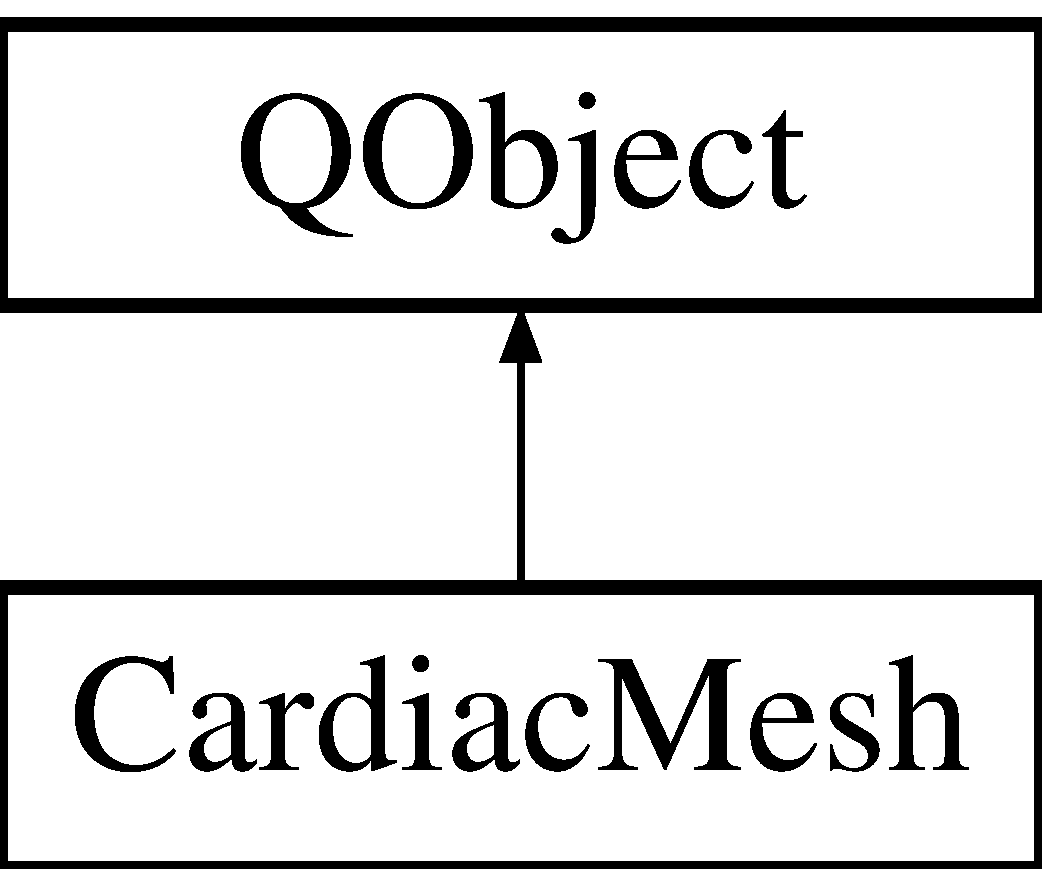
\includegraphics[height=2.000000cm]{class_cardiac_mesh}
\end{center}
\end{figure}
\subsection*{Public Slots}
\begin{DoxyCompactItemize}
\item 
int \hyperlink{class_cardiac_mesh_a5131c310815bf636bd6de60e61dc7c5e}{change\+Node} (int x, int y, \hyperlink{heart_defines_8h_a2f059cd81f362503874790462d535f5b}{C\+E\+L\+L\+\_\+\+T\+Y\+P\+E} m\+\_\+type)
\end{DoxyCompactItemize}
\subsection*{Public Member Functions}
\begin{DoxyCompactItemize}
\item 
\hyperlink{class_cardiac_mesh_a864c30e0e6cdab5e1a1e39ab99a45e5b}{Cardiac\+Mesh} ()
\item 
\hyperlink{class_cardiac_mesh_a91b0200d15669cbdef50c3d8a6ad523f}{$\sim$\+Cardiac\+Mesh} (void)
\item 
void \hyperlink{class_cardiac_mesh_ae84e8d8f86a437e47ea99d1bf212e2ce}{set\+Wall\+Cells} ()
\item 
void \hyperlink{class_cardiac_mesh_ae6002bc62e88a0a4b21ba222adc04e25}{set\+Vertex\+Triangle\+List} (bool doublesided)
\item 
void \hyperlink{class_cardiac_mesh_ac4e6a0774e1b1abf2ddbf2cc59434a92}{destroy\+Grid} ()
\item 
int \hyperlink{class_cardiac_mesh_afabd19504c5ea0168100a86205b3ccb6}{get\+Size} ()
\item 
double \hyperlink{class_cardiac_mesh_a67e146331d7c41e3d528861594ac577e}{get\+Size\+In\+Mm} ()
\item 
double \hyperlink{class_cardiac_mesh_ab4705e8f6f5657337295f076494e9a45}{get\+Delta\+R} ()
\item 
void \hyperlink{class_cardiac_mesh_a22bc3080340bc2ecad69e151098edaf5}{set\+Stimulation} (\hyperlink{class_oscillator}{Oscillator} $\ast$osc, const int \&depth)
\item 
void \hyperlink{class_cardiac_mesh_a5b11cbba123533dcf60e5bf1a7bba9cc}{stop\+Stimulation} ()
\item 
double \hyperlink{class_cardiac_mesh_abf74825fdb7bc14445c25877f06e36af}{calculate\+Electrogram} (\hyperlink{class_oscillator}{Oscillator} $\ast$osc)
\item 
void \hyperlink{class_cardiac_mesh_a92f03d96fb065ce0d12b3865182ec1b7}{calculate\+Center} ()
\end{DoxyCompactItemize}
\subsection*{Static Public Member Functions}
\begin{DoxyCompactItemize}
\item 
static \hyperlink{class_cardiac_mesh}{Cardiac\+Mesh} $\ast$ \hyperlink{class_cardiac_mesh_a1b47716c2b8eee65b46d9cd47e7abb8e}{construct\+Cartesian\+Grid} (int x, int y, double dx, double dy, \hyperlink{heart_defines_8h_a2f059cd81f362503874790462d535f5b}{C\+E\+L\+L\+\_\+\+T\+Y\+P\+E} type)
\item 
static \hyperlink{class_cardiac_mesh}{Cardiac\+Mesh} $\ast$ \hyperlink{class_cardiac_mesh_a706d5859f0b6d12d979ad6a102fc5f94}{construct\+Cylindrical\+Grid} (int x, int y, double dx, double dy)
\item 
static \hyperlink{class_cardiac_mesh}{Cardiac\+Mesh} $\ast$ \hyperlink{class_cardiac_mesh_ad0cfebe688a681428d5cb3f69d7cb839}{import\+Grid} ()
\end{DoxyCompactItemize}
\subsection*{Public Attributes}
\begin{DoxyCompactItemize}
\item 
bool \hyperlink{class_cardiac_mesh_ac14b1f228c8426e067df4a925824348e}{stimulation\+Begun}
\item 
double \hyperlink{class_cardiac_mesh_a4eeec3a9a09b9bc7e68ca3f7b34ea36c}{m\+\_\+ectopic\+Amplitude}
\item 
std\+::vector$<$ \hyperlink{class_oscillator}{Oscillator} $\ast$ $>$ \hyperlink{class_cardiac_mesh_acd49de8f8f878f45c927d4b75851ced6}{m\+\_\+mesh}
\item 
std\+::vector$<$ \hyperlink{class_oscillator}{Oscillator} $\ast$ $>$ \hyperlink{class_cardiac_mesh_a21749f0b4af8fe59552f97058982f695}{m\+\_\+under\+Stimulation}
\item 
std\+::vector$<$ std\+::pair\\*
$<$ \hyperlink{class_oscillator}{Oscillator} $\ast$, \hyperlink{class_oscillator}{Oscillator} $\ast$ $>$ $>$ \hyperlink{class_cardiac_mesh_a80e29d81b758c0294d673ae731f26343}{m\+\_\+wall\+Cells}
\item 
double \hyperlink{class_cardiac_mesh_a100654a6bb2237fc09cef29c517818ad}{m\+\_\+minimum\+Distance}
\item 
double \hyperlink{class_cardiac_mesh_a05ed4402cf331198ee5021c65ac37e23}{m\+\_\+maximum\+Distance}
\item 
double \hyperlink{class_cardiac_mesh_a48ee051becaeae6be8d4d1b1569645d2}{m\+\_\+maximum\+C\+V}
\item 
int \hyperlink{class_cardiac_mesh_aea33a4be0162859a292958757ac934fc}{m\+\_\+size}
\item 
double \hyperlink{class_cardiac_mesh_a4ebcb3d40ec7fbfea0b8f230a1677a00}{m\+\_\+radius}
\item 
std\+::vector$<$ \hyperlink{struct_vertex_triangle}{Vertex\+Triangle} $\ast$ $>$ \hyperlink{class_cardiac_mesh_a1961c25aa2da5493c0316d80c38cc088}{m\+\_\+vertex\+List}
\item 
Vector3 \hyperlink{class_cardiac_mesh_a671a783c6a63a79cc29e0b0baf8eda08}{center\+Geom}
\end{DoxyCompactItemize}


\subsection{Constructor \& Destructor Documentation}
\hypertarget{class_cardiac_mesh_a864c30e0e6cdab5e1a1e39ab99a45e5b}{\index{Cardiac\+Mesh@{Cardiac\+Mesh}!Cardiac\+Mesh@{Cardiac\+Mesh}}
\index{Cardiac\+Mesh@{Cardiac\+Mesh}!Cardiac\+Mesh@{Cardiac\+Mesh}}
\subsubsection[{Cardiac\+Mesh}]{\setlength{\rightskip}{0pt plus 5cm}Cardiac\+Mesh\+::\+Cardiac\+Mesh (
\begin{DoxyParamCaption}
{}
\end{DoxyParamCaption}
)}}\label{class_cardiac_mesh_a864c30e0e6cdab5e1a1e39ab99a45e5b}
\hypertarget{class_cardiac_mesh_a91b0200d15669cbdef50c3d8a6ad523f}{\index{Cardiac\+Mesh@{Cardiac\+Mesh}!````~Cardiac\+Mesh@{$\sim$\+Cardiac\+Mesh}}
\index{````~Cardiac\+Mesh@{$\sim$\+Cardiac\+Mesh}!Cardiac\+Mesh@{Cardiac\+Mesh}}
\subsubsection[{$\sim$\+Cardiac\+Mesh}]{\setlength{\rightskip}{0pt plus 5cm}Cardiac\+Mesh\+::$\sim$\+Cardiac\+Mesh (
\begin{DoxyParamCaption}
\item[{void}]{}
\end{DoxyParamCaption}
)}}\label{class_cardiac_mesh_a91b0200d15669cbdef50c3d8a6ad523f}


\subsection{Member Function Documentation}
\hypertarget{class_cardiac_mesh_a92f03d96fb065ce0d12b3865182ec1b7}{\index{Cardiac\+Mesh@{Cardiac\+Mesh}!calculate\+Center@{calculate\+Center}}
\index{calculate\+Center@{calculate\+Center}!Cardiac\+Mesh@{Cardiac\+Mesh}}
\subsubsection[{calculate\+Center}]{\setlength{\rightskip}{0pt plus 5cm}void Cardiac\+Mesh\+::calculate\+Center (
\begin{DoxyParamCaption}
{}
\end{DoxyParamCaption}
)}}\label{class_cardiac_mesh_a92f03d96fb065ce0d12b3865182ec1b7}
\hypertarget{class_cardiac_mesh_abf74825fdb7bc14445c25877f06e36af}{\index{Cardiac\+Mesh@{Cardiac\+Mesh}!calculate\+Electrogram@{calculate\+Electrogram}}
\index{calculate\+Electrogram@{calculate\+Electrogram}!Cardiac\+Mesh@{Cardiac\+Mesh}}
\subsubsection[{calculate\+Electrogram}]{\setlength{\rightskip}{0pt plus 5cm}double Cardiac\+Mesh\+::calculate\+Electrogram (
\begin{DoxyParamCaption}
\item[{{\bf Oscillator} $\ast$}]{osc}
\end{DoxyParamCaption}
)}}\label{class_cardiac_mesh_abf74825fdb7bc14445c25877f06e36af}
\hypertarget{class_cardiac_mesh_a5131c310815bf636bd6de60e61dc7c5e}{\index{Cardiac\+Mesh@{Cardiac\+Mesh}!change\+Node@{change\+Node}}
\index{change\+Node@{change\+Node}!Cardiac\+Mesh@{Cardiac\+Mesh}}
\subsubsection[{change\+Node}]{\setlength{\rightskip}{0pt plus 5cm}int Cardiac\+Mesh\+::change\+Node (
\begin{DoxyParamCaption}
\item[{int}]{x, }
\item[{int}]{y, }
\item[{{\bf C\+E\+L\+L\+\_\+\+T\+Y\+P\+E}}]{m\+\_\+type}
\end{DoxyParamCaption}
)\hspace{0.3cm}{\ttfamily [slot]}}}\label{class_cardiac_mesh_a5131c310815bf636bd6de60e61dc7c5e}
\hypertarget{class_cardiac_mesh_a1b47716c2b8eee65b46d9cd47e7abb8e}{\index{Cardiac\+Mesh@{Cardiac\+Mesh}!construct\+Cartesian\+Grid@{construct\+Cartesian\+Grid}}
\index{construct\+Cartesian\+Grid@{construct\+Cartesian\+Grid}!Cardiac\+Mesh@{Cardiac\+Mesh}}
\subsubsection[{construct\+Cartesian\+Grid}]{\setlength{\rightskip}{0pt plus 5cm}{\bf Cardiac\+Mesh} $\ast$ Cardiac\+Mesh\+::construct\+Cartesian\+Grid (
\begin{DoxyParamCaption}
\item[{int}]{x, }
\item[{int}]{y, }
\item[{double}]{dx, }
\item[{double}]{dy, }
\item[{{\bf C\+E\+L\+L\+\_\+\+T\+Y\+P\+E}}]{type}
\end{DoxyParamCaption}
)\hspace{0.3cm}{\ttfamily [static]}}}\label{class_cardiac_mesh_a1b47716c2b8eee65b46d9cd47e7abb8e}
\hypertarget{class_cardiac_mesh_a706d5859f0b6d12d979ad6a102fc5f94}{\index{Cardiac\+Mesh@{Cardiac\+Mesh}!construct\+Cylindrical\+Grid@{construct\+Cylindrical\+Grid}}
\index{construct\+Cylindrical\+Grid@{construct\+Cylindrical\+Grid}!Cardiac\+Mesh@{Cardiac\+Mesh}}
\subsubsection[{construct\+Cylindrical\+Grid}]{\setlength{\rightskip}{0pt plus 5cm}{\bf Cardiac\+Mesh} $\ast$ Cardiac\+Mesh\+::construct\+Cylindrical\+Grid (
\begin{DoxyParamCaption}
\item[{int}]{x, }
\item[{int}]{y, }
\item[{double}]{dx, }
\item[{double}]{dy}
\end{DoxyParamCaption}
)\hspace{0.3cm}{\ttfamily [static]}}}\label{class_cardiac_mesh_a706d5859f0b6d12d979ad6a102fc5f94}
\hypertarget{class_cardiac_mesh_ac4e6a0774e1b1abf2ddbf2cc59434a92}{\index{Cardiac\+Mesh@{Cardiac\+Mesh}!destroy\+Grid@{destroy\+Grid}}
\index{destroy\+Grid@{destroy\+Grid}!Cardiac\+Mesh@{Cardiac\+Mesh}}
\subsubsection[{destroy\+Grid}]{\setlength{\rightskip}{0pt plus 5cm}void Cardiac\+Mesh\+::destroy\+Grid (
\begin{DoxyParamCaption}
{}
\end{DoxyParamCaption}
)}}\label{class_cardiac_mesh_ac4e6a0774e1b1abf2ddbf2cc59434a92}
\hypertarget{class_cardiac_mesh_ab4705e8f6f5657337295f076494e9a45}{\index{Cardiac\+Mesh@{Cardiac\+Mesh}!get\+Delta\+R@{get\+Delta\+R}}
\index{get\+Delta\+R@{get\+Delta\+R}!Cardiac\+Mesh@{Cardiac\+Mesh}}
\subsubsection[{get\+Delta\+R}]{\setlength{\rightskip}{0pt plus 5cm}double Cardiac\+Mesh\+::get\+Delta\+R (
\begin{DoxyParamCaption}
{}
\end{DoxyParamCaption}
)}}\label{class_cardiac_mesh_ab4705e8f6f5657337295f076494e9a45}
\hypertarget{class_cardiac_mesh_afabd19504c5ea0168100a86205b3ccb6}{\index{Cardiac\+Mesh@{Cardiac\+Mesh}!get\+Size@{get\+Size}}
\index{get\+Size@{get\+Size}!Cardiac\+Mesh@{Cardiac\+Mesh}}
\subsubsection[{get\+Size}]{\setlength{\rightskip}{0pt plus 5cm}int Cardiac\+Mesh\+::get\+Size (
\begin{DoxyParamCaption}
{}
\end{DoxyParamCaption}
)}}\label{class_cardiac_mesh_afabd19504c5ea0168100a86205b3ccb6}
\hypertarget{class_cardiac_mesh_a67e146331d7c41e3d528861594ac577e}{\index{Cardiac\+Mesh@{Cardiac\+Mesh}!get\+Size\+In\+Mm@{get\+Size\+In\+Mm}}
\index{get\+Size\+In\+Mm@{get\+Size\+In\+Mm}!Cardiac\+Mesh@{Cardiac\+Mesh}}
\subsubsection[{get\+Size\+In\+Mm}]{\setlength{\rightskip}{0pt plus 5cm}double Cardiac\+Mesh\+::get\+Size\+In\+Mm (
\begin{DoxyParamCaption}
{}
\end{DoxyParamCaption}
)}}\label{class_cardiac_mesh_a67e146331d7c41e3d528861594ac577e}
\hypertarget{class_cardiac_mesh_ad0cfebe688a681428d5cb3f69d7cb839}{\index{Cardiac\+Mesh@{Cardiac\+Mesh}!import\+Grid@{import\+Grid}}
\index{import\+Grid@{import\+Grid}!Cardiac\+Mesh@{Cardiac\+Mesh}}
\subsubsection[{import\+Grid}]{\setlength{\rightskip}{0pt plus 5cm}{\bf Cardiac\+Mesh} $\ast$ Cardiac\+Mesh\+::import\+Grid (
\begin{DoxyParamCaption}
{}
\end{DoxyParamCaption}
)\hspace{0.3cm}{\ttfamily [static]}}}\label{class_cardiac_mesh_ad0cfebe688a681428d5cb3f69d7cb839}
\hypertarget{class_cardiac_mesh_a22bc3080340bc2ecad69e151098edaf5}{\index{Cardiac\+Mesh@{Cardiac\+Mesh}!set\+Stimulation@{set\+Stimulation}}
\index{set\+Stimulation@{set\+Stimulation}!Cardiac\+Mesh@{Cardiac\+Mesh}}
\subsubsection[{set\+Stimulation}]{\setlength{\rightskip}{0pt plus 5cm}void Cardiac\+Mesh\+::set\+Stimulation (
\begin{DoxyParamCaption}
\item[{{\bf Oscillator} $\ast$}]{osc, }
\item[{const int \&}]{depth}
\end{DoxyParamCaption}
)}}\label{class_cardiac_mesh_a22bc3080340bc2ecad69e151098edaf5}
\hypertarget{class_cardiac_mesh_ae6002bc62e88a0a4b21ba222adc04e25}{\index{Cardiac\+Mesh@{Cardiac\+Mesh}!set\+Vertex\+Triangle\+List@{set\+Vertex\+Triangle\+List}}
\index{set\+Vertex\+Triangle\+List@{set\+Vertex\+Triangle\+List}!Cardiac\+Mesh@{Cardiac\+Mesh}}
\subsubsection[{set\+Vertex\+Triangle\+List}]{\setlength{\rightskip}{0pt plus 5cm}void Cardiac\+Mesh\+::set\+Vertex\+Triangle\+List (
\begin{DoxyParamCaption}
\item[{bool}]{doublesided}
\end{DoxyParamCaption}
)}}\label{class_cardiac_mesh_ae6002bc62e88a0a4b21ba222adc04e25}
\hypertarget{class_cardiac_mesh_ae84e8d8f86a437e47ea99d1bf212e2ce}{\index{Cardiac\+Mesh@{Cardiac\+Mesh}!set\+Wall\+Cells@{set\+Wall\+Cells}}
\index{set\+Wall\+Cells@{set\+Wall\+Cells}!Cardiac\+Mesh@{Cardiac\+Mesh}}
\subsubsection[{set\+Wall\+Cells}]{\setlength{\rightskip}{0pt plus 5cm}void Cardiac\+Mesh\+::set\+Wall\+Cells (
\begin{DoxyParamCaption}
{}
\end{DoxyParamCaption}
)}}\label{class_cardiac_mesh_ae84e8d8f86a437e47ea99d1bf212e2ce}
\hypertarget{class_cardiac_mesh_a5b11cbba123533dcf60e5bf1a7bba9cc}{\index{Cardiac\+Mesh@{Cardiac\+Mesh}!stop\+Stimulation@{stop\+Stimulation}}
\index{stop\+Stimulation@{stop\+Stimulation}!Cardiac\+Mesh@{Cardiac\+Mesh}}
\subsubsection[{stop\+Stimulation}]{\setlength{\rightskip}{0pt plus 5cm}void Cardiac\+Mesh\+::stop\+Stimulation (
\begin{DoxyParamCaption}
{}
\end{DoxyParamCaption}
)}}\label{class_cardiac_mesh_a5b11cbba123533dcf60e5bf1a7bba9cc}


\subsection{Member Data Documentation}
\hypertarget{class_cardiac_mesh_a671a783c6a63a79cc29e0b0baf8eda08}{\index{Cardiac\+Mesh@{Cardiac\+Mesh}!center\+Geom@{center\+Geom}}
\index{center\+Geom@{center\+Geom}!Cardiac\+Mesh@{Cardiac\+Mesh}}
\subsubsection[{center\+Geom}]{\setlength{\rightskip}{0pt plus 5cm}Vector3 Cardiac\+Mesh\+::center\+Geom}}\label{class_cardiac_mesh_a671a783c6a63a79cc29e0b0baf8eda08}
\hypertarget{class_cardiac_mesh_a4eeec3a9a09b9bc7e68ca3f7b34ea36c}{\index{Cardiac\+Mesh@{Cardiac\+Mesh}!m\+\_\+ectopic\+Amplitude@{m\+\_\+ectopic\+Amplitude}}
\index{m\+\_\+ectopic\+Amplitude@{m\+\_\+ectopic\+Amplitude}!Cardiac\+Mesh@{Cardiac\+Mesh}}
\subsubsection[{m\+\_\+ectopic\+Amplitude}]{\setlength{\rightskip}{0pt plus 5cm}double Cardiac\+Mesh\+::m\+\_\+ectopic\+Amplitude}}\label{class_cardiac_mesh_a4eeec3a9a09b9bc7e68ca3f7b34ea36c}
\hypertarget{class_cardiac_mesh_a48ee051becaeae6be8d4d1b1569645d2}{\index{Cardiac\+Mesh@{Cardiac\+Mesh}!m\+\_\+maximum\+C\+V@{m\+\_\+maximum\+C\+V}}
\index{m\+\_\+maximum\+C\+V@{m\+\_\+maximum\+C\+V}!Cardiac\+Mesh@{Cardiac\+Mesh}}
\subsubsection[{m\+\_\+maximum\+C\+V}]{\setlength{\rightskip}{0pt plus 5cm}double Cardiac\+Mesh\+::m\+\_\+maximum\+C\+V}}\label{class_cardiac_mesh_a48ee051becaeae6be8d4d1b1569645d2}
\hypertarget{class_cardiac_mesh_a05ed4402cf331198ee5021c65ac37e23}{\index{Cardiac\+Mesh@{Cardiac\+Mesh}!m\+\_\+maximum\+Distance@{m\+\_\+maximum\+Distance}}
\index{m\+\_\+maximum\+Distance@{m\+\_\+maximum\+Distance}!Cardiac\+Mesh@{Cardiac\+Mesh}}
\subsubsection[{m\+\_\+maximum\+Distance}]{\setlength{\rightskip}{0pt plus 5cm}double Cardiac\+Mesh\+::m\+\_\+maximum\+Distance}}\label{class_cardiac_mesh_a05ed4402cf331198ee5021c65ac37e23}
\hypertarget{class_cardiac_mesh_acd49de8f8f878f45c927d4b75851ced6}{\index{Cardiac\+Mesh@{Cardiac\+Mesh}!m\+\_\+mesh@{m\+\_\+mesh}}
\index{m\+\_\+mesh@{m\+\_\+mesh}!Cardiac\+Mesh@{Cardiac\+Mesh}}
\subsubsection[{m\+\_\+mesh}]{\setlength{\rightskip}{0pt plus 5cm}std\+::vector$<${\bf Oscillator}$\ast$$>$ Cardiac\+Mesh\+::m\+\_\+mesh}}\label{class_cardiac_mesh_acd49de8f8f878f45c927d4b75851ced6}
\hypertarget{class_cardiac_mesh_a100654a6bb2237fc09cef29c517818ad}{\index{Cardiac\+Mesh@{Cardiac\+Mesh}!m\+\_\+minimum\+Distance@{m\+\_\+minimum\+Distance}}
\index{m\+\_\+minimum\+Distance@{m\+\_\+minimum\+Distance}!Cardiac\+Mesh@{Cardiac\+Mesh}}
\subsubsection[{m\+\_\+minimum\+Distance}]{\setlength{\rightskip}{0pt plus 5cm}double Cardiac\+Mesh\+::m\+\_\+minimum\+Distance}}\label{class_cardiac_mesh_a100654a6bb2237fc09cef29c517818ad}
\hypertarget{class_cardiac_mesh_a4ebcb3d40ec7fbfea0b8f230a1677a00}{\index{Cardiac\+Mesh@{Cardiac\+Mesh}!m\+\_\+radius@{m\+\_\+radius}}
\index{m\+\_\+radius@{m\+\_\+radius}!Cardiac\+Mesh@{Cardiac\+Mesh}}
\subsubsection[{m\+\_\+radius}]{\setlength{\rightskip}{0pt plus 5cm}double Cardiac\+Mesh\+::m\+\_\+radius}}\label{class_cardiac_mesh_a4ebcb3d40ec7fbfea0b8f230a1677a00}
\hypertarget{class_cardiac_mesh_aea33a4be0162859a292958757ac934fc}{\index{Cardiac\+Mesh@{Cardiac\+Mesh}!m\+\_\+size@{m\+\_\+size}}
\index{m\+\_\+size@{m\+\_\+size}!Cardiac\+Mesh@{Cardiac\+Mesh}}
\subsubsection[{m\+\_\+size}]{\setlength{\rightskip}{0pt plus 5cm}int Cardiac\+Mesh\+::m\+\_\+size}}\label{class_cardiac_mesh_aea33a4be0162859a292958757ac934fc}
\hypertarget{class_cardiac_mesh_a21749f0b4af8fe59552f97058982f695}{\index{Cardiac\+Mesh@{Cardiac\+Mesh}!m\+\_\+under\+Stimulation@{m\+\_\+under\+Stimulation}}
\index{m\+\_\+under\+Stimulation@{m\+\_\+under\+Stimulation}!Cardiac\+Mesh@{Cardiac\+Mesh}}
\subsubsection[{m\+\_\+under\+Stimulation}]{\setlength{\rightskip}{0pt plus 5cm}std\+::vector$<${\bf Oscillator}$\ast$$>$ Cardiac\+Mesh\+::m\+\_\+under\+Stimulation}}\label{class_cardiac_mesh_a21749f0b4af8fe59552f97058982f695}
\hypertarget{class_cardiac_mesh_a1961c25aa2da5493c0316d80c38cc088}{\index{Cardiac\+Mesh@{Cardiac\+Mesh}!m\+\_\+vertex\+List@{m\+\_\+vertex\+List}}
\index{m\+\_\+vertex\+List@{m\+\_\+vertex\+List}!Cardiac\+Mesh@{Cardiac\+Mesh}}
\subsubsection[{m\+\_\+vertex\+List}]{\setlength{\rightskip}{0pt plus 5cm}std\+::vector$<${\bf Vertex\+Triangle}$\ast$$>$ Cardiac\+Mesh\+::m\+\_\+vertex\+List}}\label{class_cardiac_mesh_a1961c25aa2da5493c0316d80c38cc088}
\hypertarget{class_cardiac_mesh_a80e29d81b758c0294d673ae731f26343}{\index{Cardiac\+Mesh@{Cardiac\+Mesh}!m\+\_\+wall\+Cells@{m\+\_\+wall\+Cells}}
\index{m\+\_\+wall\+Cells@{m\+\_\+wall\+Cells}!Cardiac\+Mesh@{Cardiac\+Mesh}}
\subsubsection[{m\+\_\+wall\+Cells}]{\setlength{\rightskip}{0pt plus 5cm}std\+::vector$<$std\+::pair$<${\bf Oscillator}$\ast$, {\bf Oscillator}$\ast$$>$ $>$ Cardiac\+Mesh\+::m\+\_\+wall\+Cells}}\label{class_cardiac_mesh_a80e29d81b758c0294d673ae731f26343}
\hypertarget{class_cardiac_mesh_ac14b1f228c8426e067df4a925824348e}{\index{Cardiac\+Mesh@{Cardiac\+Mesh}!stimulation\+Begun@{stimulation\+Begun}}
\index{stimulation\+Begun@{stimulation\+Begun}!Cardiac\+Mesh@{Cardiac\+Mesh}}
\subsubsection[{stimulation\+Begun}]{\setlength{\rightskip}{0pt plus 5cm}bool Cardiac\+Mesh\+::stimulation\+Begun}}\label{class_cardiac_mesh_ac14b1f228c8426e067df4a925824348e}


The documentation for this class was generated from the following files\+:\begin{DoxyCompactItemize}
\item 
Model/\hyperlink{_cardiac_mesh_8h}{Cardiac\+Mesh.\+h}\item 
Model/\hyperlink{_cardiac_mesh_8cpp}{Cardiac\+Mesh.\+cpp}\end{DoxyCompactItemize}

\hypertarget{class_cartesian_grid}{\section{Cartesian\+Grid Class Reference}
\label{class_cartesian_grid}\index{Cartesian\+Grid@{Cartesian\+Grid}}
}


{\ttfamily \#include $<$cartesian\+Grid.\+h$>$}

Inheritance diagram for Cartesian\+Grid\+:\begin{figure}[H]
\begin{center}
\leavevmode
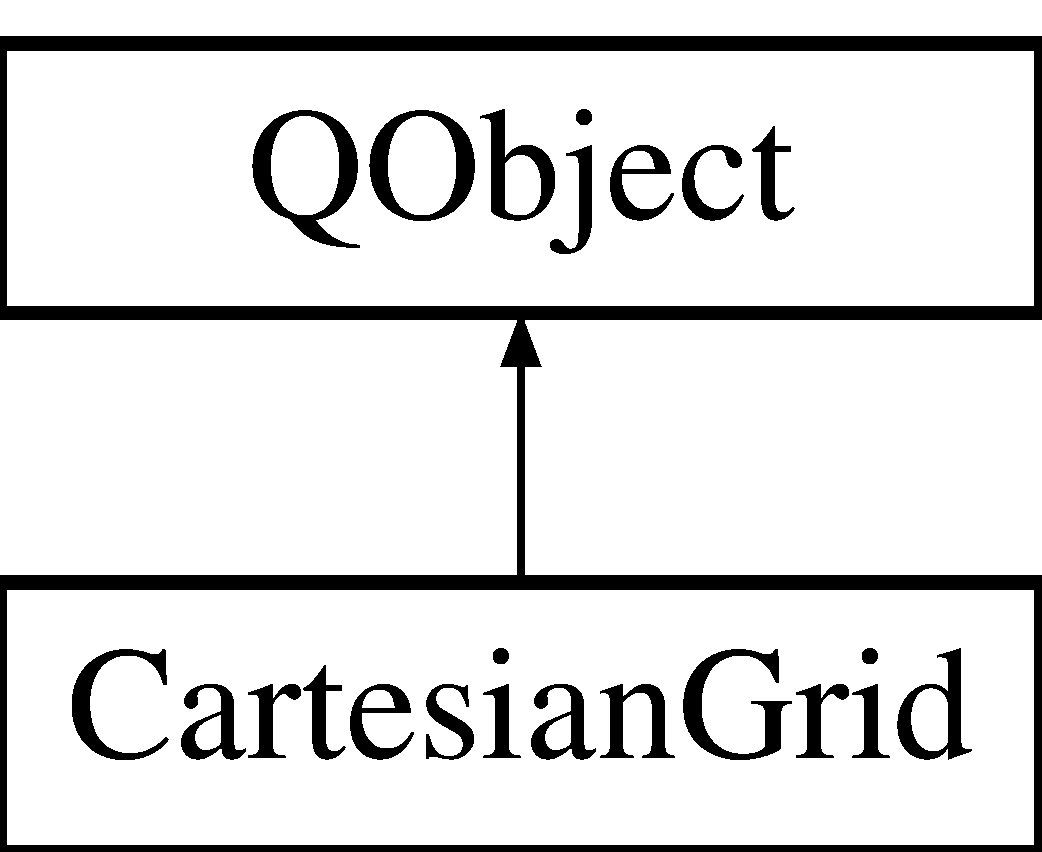
\includegraphics[height=2.000000cm]{class_cartesian_grid}
\end{center}
\end{figure}
\subsection*{Public Member Functions}
\begin{DoxyCompactItemize}
\item 
\hyperlink{class_cartesian_grid_a6d38240514f179ef0b9e88f821841aff}{Cartesian\+Grid} (int x, int y, double dx, double dy)
\item 
\hyperlink{class_cartesian_grid_aabcd0a2667fb54c3136b1aaf2d5a622a}{$\sim$\+Cartesian\+Grid} (void)
\item 
void \hyperlink{class_cartesian_grid_a60fde463ac2d4352420414cc3fb2b519}{construct\+Grid} (int x, int y, double dx, double dy)
\item 
void \hyperlink{class_cartesian_grid_a26c1bb3be5feca0f501d901000f2bbb4}{destroy\+Grid} ()
\item 
void \hyperlink{class_cartesian_grid_a8d23d0e85d3ee74135c9cf78866f45d2}{init} (int x, int y, double dx, double dy)
\item 
void \hyperlink{class_cartesian_grid_a2014b2b34c0f581f564bcbd1038d8d77}{defaults} ()
\item 
int \hyperlink{class_cartesian_grid_a7eaaf8b8392435eb7ae4bd2ce3fb0a96}{get\+Size\+X} ()
\item 
int \hyperlink{class_cartesian_grid_a18e5aa40e8b9cd1871110dc1746400b8}{get\+Size\+Y} ()
\item 
double \hyperlink{class_cartesian_grid_a2bd697548627bcc8b757bd826cd1b04f}{get\+Delta\+X} ()
\item 
double \hyperlink{class_cartesian_grid_a453f1749ef1027a4f4aa9c426bfd8cfb}{get\+Delta\+Y} ()
\end{DoxyCompactItemize}
\subsection*{Public Attributes}
\begin{DoxyCompactItemize}
\item 
std\+::vector$<$ std\+::vector$<$ \hyperlink{class_node}{Node} $\ast$ $>$ $>$ \hyperlink{class_cartesian_grid_a6c09b38347d2f1107ce12d7aef805e80}{m\+\_\+net}
\end{DoxyCompactItemize}


\subsection{Constructor \& Destructor Documentation}
\hypertarget{class_cartesian_grid_a6d38240514f179ef0b9e88f821841aff}{\index{Cartesian\+Grid@{Cartesian\+Grid}!Cartesian\+Grid@{Cartesian\+Grid}}
\index{Cartesian\+Grid@{Cartesian\+Grid}!Cartesian\+Grid@{Cartesian\+Grid}}
\subsubsection[{Cartesian\+Grid}]{\setlength{\rightskip}{0pt plus 5cm}Cartesian\+Grid\+::\+Cartesian\+Grid (
\begin{DoxyParamCaption}
\item[{int}]{x, }
\item[{int}]{y, }
\item[{double}]{dx, }
\item[{double}]{dy}
\end{DoxyParamCaption}
)}}\label{class_cartesian_grid_a6d38240514f179ef0b9e88f821841aff}
\hypertarget{class_cartesian_grid_aabcd0a2667fb54c3136b1aaf2d5a622a}{\index{Cartesian\+Grid@{Cartesian\+Grid}!````~Cartesian\+Grid@{$\sim$\+Cartesian\+Grid}}
\index{````~Cartesian\+Grid@{$\sim$\+Cartesian\+Grid}!Cartesian\+Grid@{Cartesian\+Grid}}
\subsubsection[{$\sim$\+Cartesian\+Grid}]{\setlength{\rightskip}{0pt plus 5cm}Cartesian\+Grid\+::$\sim$\+Cartesian\+Grid (
\begin{DoxyParamCaption}
\item[{void}]{}
\end{DoxyParamCaption}
)}}\label{class_cartesian_grid_aabcd0a2667fb54c3136b1aaf2d5a622a}


\subsection{Member Function Documentation}
\hypertarget{class_cartesian_grid_a60fde463ac2d4352420414cc3fb2b519}{\index{Cartesian\+Grid@{Cartesian\+Grid}!construct\+Grid@{construct\+Grid}}
\index{construct\+Grid@{construct\+Grid}!Cartesian\+Grid@{Cartesian\+Grid}}
\subsubsection[{construct\+Grid}]{\setlength{\rightskip}{0pt plus 5cm}void Cartesian\+Grid\+::construct\+Grid (
\begin{DoxyParamCaption}
\item[{int}]{x, }
\item[{int}]{y, }
\item[{double}]{dx, }
\item[{double}]{dy}
\end{DoxyParamCaption}
)}}\label{class_cartesian_grid_a60fde463ac2d4352420414cc3fb2b519}
\hypertarget{class_cartesian_grid_a2014b2b34c0f581f564bcbd1038d8d77}{\index{Cartesian\+Grid@{Cartesian\+Grid}!defaults@{defaults}}
\index{defaults@{defaults}!Cartesian\+Grid@{Cartesian\+Grid}}
\subsubsection[{defaults}]{\setlength{\rightskip}{0pt plus 5cm}void Cartesian\+Grid\+::defaults (
\begin{DoxyParamCaption}
{}
\end{DoxyParamCaption}
)}}\label{class_cartesian_grid_a2014b2b34c0f581f564bcbd1038d8d77}
\hypertarget{class_cartesian_grid_a26c1bb3be5feca0f501d901000f2bbb4}{\index{Cartesian\+Grid@{Cartesian\+Grid}!destroy\+Grid@{destroy\+Grid}}
\index{destroy\+Grid@{destroy\+Grid}!Cartesian\+Grid@{Cartesian\+Grid}}
\subsubsection[{destroy\+Grid}]{\setlength{\rightskip}{0pt plus 5cm}void Cartesian\+Grid\+::destroy\+Grid (
\begin{DoxyParamCaption}
{}
\end{DoxyParamCaption}
)}}\label{class_cartesian_grid_a26c1bb3be5feca0f501d901000f2bbb4}
\hypertarget{class_cartesian_grid_a2bd697548627bcc8b757bd826cd1b04f}{\index{Cartesian\+Grid@{Cartesian\+Grid}!get\+Delta\+X@{get\+Delta\+X}}
\index{get\+Delta\+X@{get\+Delta\+X}!Cartesian\+Grid@{Cartesian\+Grid}}
\subsubsection[{get\+Delta\+X}]{\setlength{\rightskip}{0pt plus 5cm}double Cartesian\+Grid\+::get\+Delta\+X (
\begin{DoxyParamCaption}
{}
\end{DoxyParamCaption}
)}}\label{class_cartesian_grid_a2bd697548627bcc8b757bd826cd1b04f}
\hypertarget{class_cartesian_grid_a453f1749ef1027a4f4aa9c426bfd8cfb}{\index{Cartesian\+Grid@{Cartesian\+Grid}!get\+Delta\+Y@{get\+Delta\+Y}}
\index{get\+Delta\+Y@{get\+Delta\+Y}!Cartesian\+Grid@{Cartesian\+Grid}}
\subsubsection[{get\+Delta\+Y}]{\setlength{\rightskip}{0pt plus 5cm}double Cartesian\+Grid\+::get\+Delta\+Y (
\begin{DoxyParamCaption}
{}
\end{DoxyParamCaption}
)}}\label{class_cartesian_grid_a453f1749ef1027a4f4aa9c426bfd8cfb}
\hypertarget{class_cartesian_grid_a7eaaf8b8392435eb7ae4bd2ce3fb0a96}{\index{Cartesian\+Grid@{Cartesian\+Grid}!get\+Size\+X@{get\+Size\+X}}
\index{get\+Size\+X@{get\+Size\+X}!Cartesian\+Grid@{Cartesian\+Grid}}
\subsubsection[{get\+Size\+X}]{\setlength{\rightskip}{0pt plus 5cm}int Cartesian\+Grid\+::get\+Size\+X (
\begin{DoxyParamCaption}
{}
\end{DoxyParamCaption}
)}}\label{class_cartesian_grid_a7eaaf8b8392435eb7ae4bd2ce3fb0a96}
\hypertarget{class_cartesian_grid_a18e5aa40e8b9cd1871110dc1746400b8}{\index{Cartesian\+Grid@{Cartesian\+Grid}!get\+Size\+Y@{get\+Size\+Y}}
\index{get\+Size\+Y@{get\+Size\+Y}!Cartesian\+Grid@{Cartesian\+Grid}}
\subsubsection[{get\+Size\+Y}]{\setlength{\rightskip}{0pt plus 5cm}int Cartesian\+Grid\+::get\+Size\+Y (
\begin{DoxyParamCaption}
{}
\end{DoxyParamCaption}
)}}\label{class_cartesian_grid_a18e5aa40e8b9cd1871110dc1746400b8}
\hypertarget{class_cartesian_grid_a8d23d0e85d3ee74135c9cf78866f45d2}{\index{Cartesian\+Grid@{Cartesian\+Grid}!init@{init}}
\index{init@{init}!Cartesian\+Grid@{Cartesian\+Grid}}
\subsubsection[{init}]{\setlength{\rightskip}{0pt plus 5cm}void Cartesian\+Grid\+::init (
\begin{DoxyParamCaption}
\item[{int}]{x, }
\item[{int}]{y, }
\item[{double}]{dx, }
\item[{double}]{dy}
\end{DoxyParamCaption}
)}}\label{class_cartesian_grid_a8d23d0e85d3ee74135c9cf78866f45d2}


\subsection{Member Data Documentation}
\hypertarget{class_cartesian_grid_a6c09b38347d2f1107ce12d7aef805e80}{\index{Cartesian\+Grid@{Cartesian\+Grid}!m\+\_\+net@{m\+\_\+net}}
\index{m\+\_\+net@{m\+\_\+net}!Cartesian\+Grid@{Cartesian\+Grid}}
\subsubsection[{m\+\_\+net}]{\setlength{\rightskip}{0pt plus 5cm}std\+::vector$<$std\+::vector$<${\bf Node}$\ast$$>$ $>$ Cartesian\+Grid\+::m\+\_\+net}}\label{class_cartesian_grid_a6c09b38347d2f1107ce12d7aef805e80}


The documentation for this class was generated from the following files\+:\begin{DoxyCompactItemize}
\item 
Model/\hyperlink{cartesian_grid_8h}{cartesian\+Grid.\+h}\item 
Model/\hyperlink{cartesian_grid_8cpp}{cartesian\+Grid.\+cpp}\end{DoxyCompactItemize}

\hypertarget{class_c_camera}{\section{C\+Camera Class Reference}
\label{class_c_camera}\index{C\+Camera@{C\+Camera}}
}


{\ttfamily \#include $<$G\+Lcamera.\+h$>$}

\subsection*{Public Member Functions}
\begin{DoxyCompactItemize}
\item 
void \hyperlink{class_c_camera_a072c50e18f8af53898749d006de038bf}{Move\+\_\+\+Camera} (float speed)
\item 
void \hyperlink{class_c_camera_af7b7fc6cc102a0a2df29238b93405e9c}{Raise\+\_\+\+Camera} (float speed)
\item 
void \hyperlink{class_c_camera_ab794f291bdde7dedb4502c8a30e27a44}{Strafe\+\_\+\+Camera} (float speed)
\item 
void \hyperlink{class_c_camera_adbb8fa3e17ab03f678390bfa1e291239}{Strafe\+View\+\_\+\+Camera} (float speed)
\item 
void \hyperlink{class_c_camera_a77ecbd62fe41b04938a51d51ce07da26}{Position\+\_\+\+Camera} (float pos\+\_\+x, float pos\+\_\+y, float pos\+\_\+z, float view\+\_\+x, float view\+\_\+y, float view\+\_\+z, float up\+\_\+x, float up\+\_\+y, float up\+\_\+z)
\end{DoxyCompactItemize}
\subsection*{Public Attributes}
\begin{DoxyCompactItemize}
\item 
\hyperlink{structt_vector3}{t\+Vector3} \hyperlink{class_c_camera_ab38cdbfdbb298cbaf93d1982112d4091}{m\+Pos}
\item 
\hyperlink{structt_vector3}{t\+Vector3} \hyperlink{class_c_camera_a7014fff6f0458dae9b5f97ecdb5e3ab0}{m\+View}
\item 
\hyperlink{structt_vector3}{t\+Vector3} \hyperlink{class_c_camera_a95a552f343e871b3afd969b39781b04d}{m\+Up}
\end{DoxyCompactItemize}


\subsection{Member Function Documentation}
\hypertarget{class_c_camera_a072c50e18f8af53898749d006de038bf}{\index{C\+Camera@{C\+Camera}!Move\+\_\+\+Camera@{Move\+\_\+\+Camera}}
\index{Move\+\_\+\+Camera@{Move\+\_\+\+Camera}!C\+Camera@{C\+Camera}}
\subsubsection[{Move\+\_\+\+Camera}]{\setlength{\rightskip}{0pt plus 5cm}void C\+Camera\+::\+Move\+\_\+\+Camera (
\begin{DoxyParamCaption}
\item[{float}]{speed}
\end{DoxyParamCaption}
)}}\label{class_c_camera_a072c50e18f8af53898749d006de038bf}
\hypertarget{class_c_camera_a77ecbd62fe41b04938a51d51ce07da26}{\index{C\+Camera@{C\+Camera}!Position\+\_\+\+Camera@{Position\+\_\+\+Camera}}
\index{Position\+\_\+\+Camera@{Position\+\_\+\+Camera}!C\+Camera@{C\+Camera}}
\subsubsection[{Position\+\_\+\+Camera}]{\setlength{\rightskip}{0pt plus 5cm}void C\+Camera\+::\+Position\+\_\+\+Camera (
\begin{DoxyParamCaption}
\item[{float}]{pos\+\_\+x, }
\item[{float}]{pos\+\_\+y, }
\item[{float}]{pos\+\_\+z, }
\item[{float}]{view\+\_\+x, }
\item[{float}]{view\+\_\+y, }
\item[{float}]{view\+\_\+z, }
\item[{float}]{up\+\_\+x, }
\item[{float}]{up\+\_\+y, }
\item[{float}]{up\+\_\+z}
\end{DoxyParamCaption}
)}}\label{class_c_camera_a77ecbd62fe41b04938a51d51ce07da26}
\hypertarget{class_c_camera_af7b7fc6cc102a0a2df29238b93405e9c}{\index{C\+Camera@{C\+Camera}!Raise\+\_\+\+Camera@{Raise\+\_\+\+Camera}}
\index{Raise\+\_\+\+Camera@{Raise\+\_\+\+Camera}!C\+Camera@{C\+Camera}}
\subsubsection[{Raise\+\_\+\+Camera}]{\setlength{\rightskip}{0pt plus 5cm}void C\+Camera\+::\+Raise\+\_\+\+Camera (
\begin{DoxyParamCaption}
\item[{float}]{speed}
\end{DoxyParamCaption}
)}}\label{class_c_camera_af7b7fc6cc102a0a2df29238b93405e9c}
m\+Pos.\+z = m\+Pos.\+z + v\+Vector.\+z $\ast$ speed; \hypertarget{class_c_camera_ab794f291bdde7dedb4502c8a30e27a44}{\index{C\+Camera@{C\+Camera}!Strafe\+\_\+\+Camera@{Strafe\+\_\+\+Camera}}
\index{Strafe\+\_\+\+Camera@{Strafe\+\_\+\+Camera}!C\+Camera@{C\+Camera}}
\subsubsection[{Strafe\+\_\+\+Camera}]{\setlength{\rightskip}{0pt plus 5cm}void C\+Camera\+::\+Strafe\+\_\+\+Camera (
\begin{DoxyParamCaption}
\item[{float}]{speed}
\end{DoxyParamCaption}
)}}\label{class_c_camera_ab794f291bdde7dedb4502c8a30e27a44}
\hypertarget{class_c_camera_adbb8fa3e17ab03f678390bfa1e291239}{\index{C\+Camera@{C\+Camera}!Strafe\+View\+\_\+\+Camera@{Strafe\+View\+\_\+\+Camera}}
\index{Strafe\+View\+\_\+\+Camera@{Strafe\+View\+\_\+\+Camera}!C\+Camera@{C\+Camera}}
\subsubsection[{Strafe\+View\+\_\+\+Camera}]{\setlength{\rightskip}{0pt plus 5cm}void C\+Camera\+::\+Strafe\+View\+\_\+\+Camera (
\begin{DoxyParamCaption}
\item[{float}]{speed}
\end{DoxyParamCaption}
)}}\label{class_c_camera_adbb8fa3e17ab03f678390bfa1e291239}


\subsection{Member Data Documentation}
\hypertarget{class_c_camera_ab38cdbfdbb298cbaf93d1982112d4091}{\index{C\+Camera@{C\+Camera}!m\+Pos@{m\+Pos}}
\index{m\+Pos@{m\+Pos}!C\+Camera@{C\+Camera}}
\subsubsection[{m\+Pos}]{\setlength{\rightskip}{0pt plus 5cm}{\bf t\+Vector3} C\+Camera\+::m\+Pos}}\label{class_c_camera_ab38cdbfdbb298cbaf93d1982112d4091}
\hypertarget{class_c_camera_a95a552f343e871b3afd969b39781b04d}{\index{C\+Camera@{C\+Camera}!m\+Up@{m\+Up}}
\index{m\+Up@{m\+Up}!C\+Camera@{C\+Camera}}
\subsubsection[{m\+Up}]{\setlength{\rightskip}{0pt plus 5cm}{\bf t\+Vector3} C\+Camera\+::m\+Up}}\label{class_c_camera_a95a552f343e871b3afd969b39781b04d}
\hypertarget{class_c_camera_a7014fff6f0458dae9b5f97ecdb5e3ab0}{\index{C\+Camera@{C\+Camera}!m\+View@{m\+View}}
\index{m\+View@{m\+View}!C\+Camera@{C\+Camera}}
\subsubsection[{m\+View}]{\setlength{\rightskip}{0pt plus 5cm}{\bf t\+Vector3} C\+Camera\+::m\+View}}\label{class_c_camera_a7014fff6f0458dae9b5f97ecdb5e3ab0}


The documentation for this class was generated from the following files\+:\begin{DoxyCompactItemize}
\item 
\hyperlink{_g_lcamera_8h}{G\+Lcamera.\+h}\item 
\hyperlink{_g_lcamera_8cpp}{G\+Lcamera.\+cpp}\end{DoxyCompactItemize}

\hypertarget{structcompare___timestep_node}{\section{compare\+\_\+\+Timestep\+Node Struct Reference}
\label{structcompare___timestep_node}\index{compare\+\_\+\+Timestep\+Node@{compare\+\_\+\+Timestep\+Node}}
}


{\ttfamily \#include $<$Timestep\+Node.\+h$>$}

\subsection*{Public Member Functions}
\begin{DoxyCompactItemize}
\item 
bool \hyperlink{structcompare___timestep_node_a5fc38bc5563b980f7a995da9bc427f4d}{operator()} (const \hyperlink{struct_timestep_node}{Timestep\+Node} $\ast$const \&n1, const \hyperlink{struct_timestep_node}{Timestep\+Node} $\ast$const \&n2) const 
\end{DoxyCompactItemize}


\subsection{Member Function Documentation}
\hypertarget{structcompare___timestep_node_a5fc38bc5563b980f7a995da9bc427f4d}{\index{compare\+\_\+\+Timestep\+Node@{compare\+\_\+\+Timestep\+Node}!operator()@{operator()}}
\index{operator()@{operator()}!compare\+\_\+\+Timestep\+Node@{compare\+\_\+\+Timestep\+Node}}
\subsubsection[{operator()}]{\setlength{\rightskip}{0pt plus 5cm}bool compare\+\_\+\+Timestep\+Node\+::operator() (
\begin{DoxyParamCaption}
\item[{const {\bf Timestep\+Node} $\ast$const \&}]{n1, }
\item[{const {\bf Timestep\+Node} $\ast$const \&}]{n2}
\end{DoxyParamCaption}
) const\hspace{0.3cm}{\ttfamily [inline]}}}\label{structcompare___timestep_node_a5fc38bc5563b980f7a995da9bc427f4d}


The documentation for this struct was generated from the following file\+:\begin{DoxyCompactItemize}
\item 
Numeric\+Strategy/\hyperlink{_timestep_node_8h}{Timestep\+Node.\+h}\end{DoxyCompactItemize}

\hypertarget{class_curve_data}{\section{Curve\+Data Class Reference}
\label{class_curve_data}\index{Curve\+Data@{Curve\+Data}}
}


{\ttfamily \#include $<$Curve\+Data.\+h$>$}

\subsection*{Public Member Functions}
\begin{DoxyCompactItemize}
\item 
\hyperlink{class_curve_data_a4e9a1bb778f0cb2e7d573b88163cfd38}{Curve\+Data} ()
\item 
void \hyperlink{class_curve_data_aa5a619af9980fa45612c98d438444b07}{append} (double $\ast$\hyperlink{class_curve_data_aeb1b65fe291fe72fa363640245383da4}{x}, double $\ast$\hyperlink{class_curve_data_a681ce130c86c62bcc1f6c488645f9b5b}{y}, int \hyperlink{class_curve_data_a6d3c0bbc2069cc39f265aa8e9ee5ad73}{count})
\item 
int \hyperlink{class_curve_data_a6d3c0bbc2069cc39f265aa8e9ee5ad73}{count} () const 
\item 
int \hyperlink{class_curve_data_aa47747f11e103e908781800b278596d7}{size} () const 
\item 
const double $\ast$ \hyperlink{class_curve_data_aeb1b65fe291fe72fa363640245383da4}{x} () const 
\item 
const double $\ast$ \hyperlink{class_curve_data_a681ce130c86c62bcc1f6c488645f9b5b}{y} () const 
\item 
void \hyperlink{class_curve_data_ae898810872a274a681ab60131ecf922b}{clear} ()
\end{DoxyCompactItemize}


\subsection{Constructor \& Destructor Documentation}
\hypertarget{class_curve_data_a4e9a1bb778f0cb2e7d573b88163cfd38}{\index{Curve\+Data@{Curve\+Data}!Curve\+Data@{Curve\+Data}}
\index{Curve\+Data@{Curve\+Data}!Curve\+Data@{Curve\+Data}}
\subsubsection[{Curve\+Data}]{\setlength{\rightskip}{0pt plus 5cm}Curve\+Data\+::\+Curve\+Data (
\begin{DoxyParamCaption}
{}
\end{DoxyParamCaption}
)}}\label{class_curve_data_a4e9a1bb778f0cb2e7d573b88163cfd38}


\subsection{Member Function Documentation}
\hypertarget{class_curve_data_aa5a619af9980fa45612c98d438444b07}{\index{Curve\+Data@{Curve\+Data}!append@{append}}
\index{append@{append}!Curve\+Data@{Curve\+Data}}
\subsubsection[{append}]{\setlength{\rightskip}{0pt plus 5cm}void Curve\+Data\+::append (
\begin{DoxyParamCaption}
\item[{double $\ast$}]{x, }
\item[{double $\ast$}]{y, }
\item[{int}]{count}
\end{DoxyParamCaption}
)}}\label{class_curve_data_aa5a619af9980fa45612c98d438444b07}
\hypertarget{class_curve_data_ae898810872a274a681ab60131ecf922b}{\index{Curve\+Data@{Curve\+Data}!clear@{clear}}
\index{clear@{clear}!Curve\+Data@{Curve\+Data}}
\subsubsection[{clear}]{\setlength{\rightskip}{0pt plus 5cm}void Curve\+Data\+::clear (
\begin{DoxyParamCaption}
{}
\end{DoxyParamCaption}
)}}\label{class_curve_data_ae898810872a274a681ab60131ecf922b}
\hypertarget{class_curve_data_a6d3c0bbc2069cc39f265aa8e9ee5ad73}{\index{Curve\+Data@{Curve\+Data}!count@{count}}
\index{count@{count}!Curve\+Data@{Curve\+Data}}
\subsubsection[{count}]{\setlength{\rightskip}{0pt plus 5cm}int Curve\+Data\+::count (
\begin{DoxyParamCaption}
{}
\end{DoxyParamCaption}
) const}}\label{class_curve_data_a6d3c0bbc2069cc39f265aa8e9ee5ad73}
\hypertarget{class_curve_data_aa47747f11e103e908781800b278596d7}{\index{Curve\+Data@{Curve\+Data}!size@{size}}
\index{size@{size}!Curve\+Data@{Curve\+Data}}
\subsubsection[{size}]{\setlength{\rightskip}{0pt plus 5cm}int Curve\+Data\+::size (
\begin{DoxyParamCaption}
{}
\end{DoxyParamCaption}
) const}}\label{class_curve_data_aa47747f11e103e908781800b278596d7}
\hypertarget{class_curve_data_aeb1b65fe291fe72fa363640245383da4}{\index{Curve\+Data@{Curve\+Data}!x@{x}}
\index{x@{x}!Curve\+Data@{Curve\+Data}}
\subsubsection[{x}]{\setlength{\rightskip}{0pt plus 5cm}const double $\ast$ Curve\+Data\+::x (
\begin{DoxyParamCaption}
{}
\end{DoxyParamCaption}
) const}}\label{class_curve_data_aeb1b65fe291fe72fa363640245383da4}
\hypertarget{class_curve_data_a681ce130c86c62bcc1f6c488645f9b5b}{\index{Curve\+Data@{Curve\+Data}!y@{y}}
\index{y@{y}!Curve\+Data@{Curve\+Data}}
\subsubsection[{y}]{\setlength{\rightskip}{0pt plus 5cm}const double $\ast$ Curve\+Data\+::y (
\begin{DoxyParamCaption}
{}
\end{DoxyParamCaption}
) const}}\label{class_curve_data_a681ce130c86c62bcc1f6c488645f9b5b}


The documentation for this class was generated from the following files\+:\begin{DoxyCompactItemize}
\item 
\hyperlink{_curve_data_8h}{Curve\+Data.\+h}\item 
\hyperlink{_curve_data_8cpp}{Curve\+Data.\+cpp}\end{DoxyCompactItemize}

\hypertarget{class_default_plot}{\section{Default\+Plot Class Reference}
\label{class_default_plot}\index{Default\+Plot@{Default\+Plot}}
}


{\ttfamily \#include $<$default\+Plot.\+h$>$}

Inheritance diagram for Default\+Plot\+:\begin{figure}[H]
\begin{center}
\leavevmode
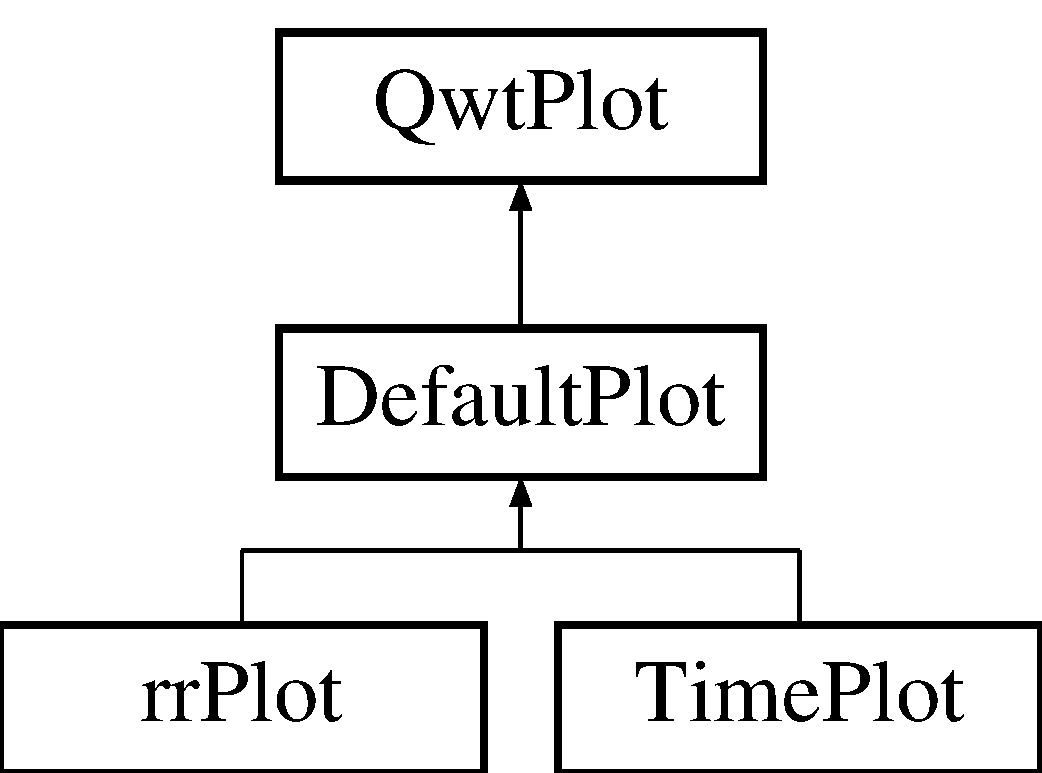
\includegraphics[height=3.000000cm]{class_default_plot}
\end{center}
\end{figure}
\subsection*{Public Slots}
\begin{DoxyCompactItemize}
\item 
void \hyperlink{class_default_plot_a854d9542172051ce35f1a0c4feb53f33}{append\+Data} (double x, double y, int curve\+\_\+id)
\item 
void \hyperlink{class_default_plot_acff90f7cdbbd829abfca06ed24507da7}{append\+Data} (double $\ast$x, double $\ast$y, int size, int curve\+\_\+id)
\item 
void \hyperlink{class_default_plot_a1b738fc1cee258914b5cccbd63131ace}{set\+Scale\+Min\+X} (double min\+\_\+\+Range\+X)
\item 
void \hyperlink{class_default_plot_adb1b7d66e42b376734a4e2be176f3382}{set\+Scale\+Max\+X} (double max\+\_\+\+Range\+X)
\item 
void \hyperlink{class_default_plot_aa0924bd27c05af6d656301afe2e25851}{set\+Scale\+Min\+Y} (double min\+\_\+\+Range\+Y)
\item 
void \hyperlink{class_default_plot_aebaa780d70e4b8fe39a83da2939ea2b2}{set\+Scale\+Max\+Y} (double max\+\_\+\+Range\+Y)
\item 
void \hyperlink{class_default_plot_a64d7ce1a40eb783f9ebc34b8f5229fca}{move\+Left\+Mark} (Q\+Point pos)
\item 
void \hyperlink{class_default_plot_ab61e442a78117779faf7594af03352fa}{move\+Right\+Mark} (Q\+Point pos)
\item 
void \hyperlink{class_default_plot_ad5983e28b973fa6050d1d38243c4d18d}{clear} ()
\item 
void \hyperlink{class_default_plot_a1ece166f6f9da202fbbbd87a3276ec91}{mouse\+Press\+Event} (Q\+Mouse\+Event $\ast$event)
\end{DoxyCompactItemize}
\subsection*{Public Member Functions}
\begin{DoxyCompactItemize}
\item 
\hyperlink{class_default_plot_a121e294348cf317ccb4eaa8725aa2a6f}{Default\+Plot} (Q\+Widget $\ast$parent)
\item 
virtual \hyperlink{class_default_plot_a102c42148b1e4c49dd77d0e4cf8cb05a}{$\sim$\+Default\+Plot} (void)
\item 
void \hyperlink{class_default_plot_ac66f2cf5b8bf20358add7261df109c9b}{remove\+Data} ()
\item 
unsigned int \hyperlink{class_default_plot_a5c9b858cc4b0b916a2f38e19cb4387c0}{add\+Curve} (std\+::string name, Q\+Color color)
\item 
void \hyperlink{class_default_plot_a572dcb659361187315a0beac070ab7f0}{remove\+Curve} ()
\item 
void \hyperlink{class_default_plot_a4d68b948dd93d81b37e3c1c39a5f29ce}{set\+Axis\+Max\+Range\+X} (double minx, double maxx)
\item 
void \hyperlink{class_default_plot_a98b4626122852228be88a4adf7b78929}{set\+Axis\+Max\+Range\+Y} (double miny, double maxy)
\end{DoxyCompactItemize}
\subsection*{Public Attributes}
\begin{DoxyCompactItemize}
\item 
std\+::vector$<$ \hyperlink{class_curve_data}{Curve\+Data} $\ast$ $>$ \hyperlink{class_default_plot_aa78c1b3ad9d6328731ecae5a27b9d0b1}{d\+\_\+data}
\item 
Qwt\+Symbol $\ast$ \hyperlink{class_default_plot_a30118ba9670ca7bf1c852e98bf76771a}{s}
\item 
std\+::vector$<$ Qwt\+Plot\+Curve $\ast$ $>$ \hyperlink{class_default_plot_a154b2bb7e4528185f88ff204da70e4de}{d\+\_\+curve}
\end{DoxyCompactItemize}
\subsection*{Protected Member Functions}
\begin{DoxyCompactItemize}
\item 
void \hyperlink{class_default_plot_ab58ec19e4da4991a5ef9e04f3cc1f24e}{align\+Scales} ()
\end{DoxyCompactItemize}
\subsection*{Protected Attributes}
\begin{DoxyCompactItemize}
\item 
double \hyperlink{class_default_plot_ad9c7fefd2b2beac187116c6c274e226b}{max\+Range\+X}
\item 
double \hyperlink{class_default_plot_a5fb55a0fc4fb764c9ab100ef8bed151a}{min\+Range\+X}
\item 
double \hyperlink{class_default_plot_a0a9fd99e0ffac64fbbe8e2c7d599699d}{max\+Range\+Y}
\item 
double \hyperlink{class_default_plot_a6430390e18d83bcd55212e7a56af7cb3}{min\+Range\+Y}
\item 
Qwt\+Text \hyperlink{class_default_plot_aecabd8aa4a721d21e1e01dcc41c621ea}{current\+Text}
\item 
Qwt\+Legend $\ast$ \hyperlink{class_default_plot_a599dcc2f358a4d1f7500a00018b4ba9d}{legend}
\item 
Qwt\+Plot\+Grid $\ast$ \hyperlink{class_default_plot_a7bf0ea1a18ef87f69aaab57589629da4}{grid}
\item 
Qwt\+Plot\+Marker $\ast$ \hyperlink{class_default_plot_ada5a5d4e6f0996d79b0a4ba353f12726}{d\+\_\+mrk1}
\item 
Qwt\+Plot\+Marker $\ast$ \hyperlink{class_default_plot_a8021357960017f7338d48981e32b8ae4}{d\+\_\+mrk2}
\item 
Qwt\+Plot\+Picker $\ast$ \hyperlink{class_default_plot_afc5eba9a9ff1a5fa825fd34dc5637b68}{d\+\_\+picker}
\item 
\hyperlink{classatrial_parameters}{atrial\+Parameters} \hyperlink{class_default_plot_a2c81cca14d02f5c3802f462f84ba2864}{m\+\_\+defines}
\end{DoxyCompactItemize}


\subsection{Constructor \& Destructor Documentation}
\hypertarget{class_default_plot_a121e294348cf317ccb4eaa8725aa2a6f}{\index{Default\+Plot@{Default\+Plot}!Default\+Plot@{Default\+Plot}}
\index{Default\+Plot@{Default\+Plot}!Default\+Plot@{Default\+Plot}}
\subsubsection[{Default\+Plot}]{\setlength{\rightskip}{0pt plus 5cm}Default\+Plot\+::\+Default\+Plot (
\begin{DoxyParamCaption}
\item[{Q\+Widget $\ast$}]{parent}
\end{DoxyParamCaption}
)}}\label{class_default_plot_a121e294348cf317ccb4eaa8725aa2a6f}
\hypertarget{class_default_plot_a102c42148b1e4c49dd77d0e4cf8cb05a}{\index{Default\+Plot@{Default\+Plot}!````~Default\+Plot@{$\sim$\+Default\+Plot}}
\index{````~Default\+Plot@{$\sim$\+Default\+Plot}!Default\+Plot@{Default\+Plot}}
\subsubsection[{$\sim$\+Default\+Plot}]{\setlength{\rightskip}{0pt plus 5cm}Default\+Plot\+::$\sim$\+Default\+Plot (
\begin{DoxyParamCaption}
\item[{void}]{}
\end{DoxyParamCaption}
)\hspace{0.3cm}{\ttfamily [virtual]}}}\label{class_default_plot_a102c42148b1e4c49dd77d0e4cf8cb05a}


\subsection{Member Function Documentation}
\hypertarget{class_default_plot_a5c9b858cc4b0b916a2f38e19cb4387c0}{\index{Default\+Plot@{Default\+Plot}!add\+Curve@{add\+Curve}}
\index{add\+Curve@{add\+Curve}!Default\+Plot@{Default\+Plot}}
\subsubsection[{add\+Curve}]{\setlength{\rightskip}{0pt plus 5cm}unsigned int Default\+Plot\+::add\+Curve (
\begin{DoxyParamCaption}
\item[{std\+::string}]{name, }
\item[{Q\+Color}]{color}
\end{DoxyParamCaption}
)}}\label{class_default_plot_a5c9b858cc4b0b916a2f38e19cb4387c0}
\hypertarget{class_default_plot_ab58ec19e4da4991a5ef9e04f3cc1f24e}{\index{Default\+Plot@{Default\+Plot}!align\+Scales@{align\+Scales}}
\index{align\+Scales@{align\+Scales}!Default\+Plot@{Default\+Plot}}
\subsubsection[{align\+Scales}]{\setlength{\rightskip}{0pt plus 5cm}void Default\+Plot\+::align\+Scales (
\begin{DoxyParamCaption}
{}
\end{DoxyParamCaption}
)\hspace{0.3cm}{\ttfamily [protected]}}}\label{class_default_plot_ab58ec19e4da4991a5ef9e04f3cc1f24e}
\hypertarget{class_default_plot_a854d9542172051ce35f1a0c4feb53f33}{\index{Default\+Plot@{Default\+Plot}!append\+Data@{append\+Data}}
\index{append\+Data@{append\+Data}!Default\+Plot@{Default\+Plot}}
\subsubsection[{append\+Data}]{\setlength{\rightskip}{0pt plus 5cm}void Default\+Plot\+::append\+Data (
\begin{DoxyParamCaption}
\item[{double}]{x, }
\item[{double}]{y, }
\item[{int}]{curve\+\_\+id}
\end{DoxyParamCaption}
)\hspace{0.3cm}{\ttfamily [slot]}}}\label{class_default_plot_a854d9542172051ce35f1a0c4feb53f33}
\hypertarget{class_default_plot_acff90f7cdbbd829abfca06ed24507da7}{\index{Default\+Plot@{Default\+Plot}!append\+Data@{append\+Data}}
\index{append\+Data@{append\+Data}!Default\+Plot@{Default\+Plot}}
\subsubsection[{append\+Data}]{\setlength{\rightskip}{0pt plus 5cm}void Default\+Plot\+::append\+Data (
\begin{DoxyParamCaption}
\item[{double $\ast$}]{x, }
\item[{double $\ast$}]{y, }
\item[{int}]{size, }
\item[{int}]{curve\+\_\+id}
\end{DoxyParamCaption}
)\hspace{0.3cm}{\ttfamily [slot]}}}\label{class_default_plot_acff90f7cdbbd829abfca06ed24507da7}
\hypertarget{class_default_plot_ad5983e28b973fa6050d1d38243c4d18d}{\index{Default\+Plot@{Default\+Plot}!clear@{clear}}
\index{clear@{clear}!Default\+Plot@{Default\+Plot}}
\subsubsection[{clear}]{\setlength{\rightskip}{0pt plus 5cm}void Default\+Plot\+::clear (
\begin{DoxyParamCaption}
{}
\end{DoxyParamCaption}
)\hspace{0.3cm}{\ttfamily [slot]}}}\label{class_default_plot_ad5983e28b973fa6050d1d38243c4d18d}
\hypertarget{class_default_plot_a1ece166f6f9da202fbbbd87a3276ec91}{\index{Default\+Plot@{Default\+Plot}!mouse\+Press\+Event@{mouse\+Press\+Event}}
\index{mouse\+Press\+Event@{mouse\+Press\+Event}!Default\+Plot@{Default\+Plot}}
\subsubsection[{mouse\+Press\+Event}]{\setlength{\rightskip}{0pt plus 5cm}void Default\+Plot\+::mouse\+Press\+Event (
\begin{DoxyParamCaption}
\item[{Q\+Mouse\+Event $\ast$}]{event}
\end{DoxyParamCaption}
)\hspace{0.3cm}{\ttfamily [slot]}}}\label{class_default_plot_a1ece166f6f9da202fbbbd87a3276ec91}
\hypertarget{class_default_plot_a64d7ce1a40eb783f9ebc34b8f5229fca}{\index{Default\+Plot@{Default\+Plot}!move\+Left\+Mark@{move\+Left\+Mark}}
\index{move\+Left\+Mark@{move\+Left\+Mark}!Default\+Plot@{Default\+Plot}}
\subsubsection[{move\+Left\+Mark}]{\setlength{\rightskip}{0pt plus 5cm}void Default\+Plot\+::move\+Left\+Mark (
\begin{DoxyParamCaption}
\item[{Q\+Point}]{pos}
\end{DoxyParamCaption}
)\hspace{0.3cm}{\ttfamily [slot]}}}\label{class_default_plot_a64d7ce1a40eb783f9ebc34b8f5229fca}
\hypertarget{class_default_plot_ab61e442a78117779faf7594af03352fa}{\index{Default\+Plot@{Default\+Plot}!move\+Right\+Mark@{move\+Right\+Mark}}
\index{move\+Right\+Mark@{move\+Right\+Mark}!Default\+Plot@{Default\+Plot}}
\subsubsection[{move\+Right\+Mark}]{\setlength{\rightskip}{0pt plus 5cm}void Default\+Plot\+::move\+Right\+Mark (
\begin{DoxyParamCaption}
\item[{Q\+Point}]{pos}
\end{DoxyParamCaption}
)\hspace{0.3cm}{\ttfamily [slot]}}}\label{class_default_plot_ab61e442a78117779faf7594af03352fa}
\hypertarget{class_default_plot_a572dcb659361187315a0beac070ab7f0}{\index{Default\+Plot@{Default\+Plot}!remove\+Curve@{remove\+Curve}}
\index{remove\+Curve@{remove\+Curve}!Default\+Plot@{Default\+Plot}}
\subsubsection[{remove\+Curve}]{\setlength{\rightskip}{0pt plus 5cm}void Default\+Plot\+::remove\+Curve (
\begin{DoxyParamCaption}
{}
\end{DoxyParamCaption}
)}}\label{class_default_plot_a572dcb659361187315a0beac070ab7f0}
\hypertarget{class_default_plot_ac66f2cf5b8bf20358add7261df109c9b}{\index{Default\+Plot@{Default\+Plot}!remove\+Data@{remove\+Data}}
\index{remove\+Data@{remove\+Data}!Default\+Plot@{Default\+Plot}}
\subsubsection[{remove\+Data}]{\setlength{\rightskip}{0pt plus 5cm}void Default\+Plot\+::remove\+Data (
\begin{DoxyParamCaption}
{}
\end{DoxyParamCaption}
)}}\label{class_default_plot_ac66f2cf5b8bf20358add7261df109c9b}
\hypertarget{class_default_plot_a4d68b948dd93d81b37e3c1c39a5f29ce}{\index{Default\+Plot@{Default\+Plot}!set\+Axis\+Max\+Range\+X@{set\+Axis\+Max\+Range\+X}}
\index{set\+Axis\+Max\+Range\+X@{set\+Axis\+Max\+Range\+X}!Default\+Plot@{Default\+Plot}}
\subsubsection[{set\+Axis\+Max\+Range\+X}]{\setlength{\rightskip}{0pt plus 5cm}void Default\+Plot\+::set\+Axis\+Max\+Range\+X (
\begin{DoxyParamCaption}
\item[{double}]{minx, }
\item[{double}]{maxx}
\end{DoxyParamCaption}
)}}\label{class_default_plot_a4d68b948dd93d81b37e3c1c39a5f29ce}
\hypertarget{class_default_plot_a98b4626122852228be88a4adf7b78929}{\index{Default\+Plot@{Default\+Plot}!set\+Axis\+Max\+Range\+Y@{set\+Axis\+Max\+Range\+Y}}
\index{set\+Axis\+Max\+Range\+Y@{set\+Axis\+Max\+Range\+Y}!Default\+Plot@{Default\+Plot}}
\subsubsection[{set\+Axis\+Max\+Range\+Y}]{\setlength{\rightskip}{0pt plus 5cm}void Default\+Plot\+::set\+Axis\+Max\+Range\+Y (
\begin{DoxyParamCaption}
\item[{double}]{miny, }
\item[{double}]{maxy}
\end{DoxyParamCaption}
)}}\label{class_default_plot_a98b4626122852228be88a4adf7b78929}
\hypertarget{class_default_plot_adb1b7d66e42b376734a4e2be176f3382}{\index{Default\+Plot@{Default\+Plot}!set\+Scale\+Max\+X@{set\+Scale\+Max\+X}}
\index{set\+Scale\+Max\+X@{set\+Scale\+Max\+X}!Default\+Plot@{Default\+Plot}}
\subsubsection[{set\+Scale\+Max\+X}]{\setlength{\rightskip}{0pt plus 5cm}void Default\+Plot\+::set\+Scale\+Max\+X (
\begin{DoxyParamCaption}
\item[{double}]{max\+\_\+\+Range\+X}
\end{DoxyParamCaption}
)\hspace{0.3cm}{\ttfamily [slot]}}}\label{class_default_plot_adb1b7d66e42b376734a4e2be176f3382}
\hypertarget{class_default_plot_aebaa780d70e4b8fe39a83da2939ea2b2}{\index{Default\+Plot@{Default\+Plot}!set\+Scale\+Max\+Y@{set\+Scale\+Max\+Y}}
\index{set\+Scale\+Max\+Y@{set\+Scale\+Max\+Y}!Default\+Plot@{Default\+Plot}}
\subsubsection[{set\+Scale\+Max\+Y}]{\setlength{\rightskip}{0pt plus 5cm}void Default\+Plot\+::set\+Scale\+Max\+Y (
\begin{DoxyParamCaption}
\item[{double}]{max\+\_\+\+Range\+Y}
\end{DoxyParamCaption}
)\hspace{0.3cm}{\ttfamily [slot]}}}\label{class_default_plot_aebaa780d70e4b8fe39a83da2939ea2b2}
\hypertarget{class_default_plot_a1b738fc1cee258914b5cccbd63131ace}{\index{Default\+Plot@{Default\+Plot}!set\+Scale\+Min\+X@{set\+Scale\+Min\+X}}
\index{set\+Scale\+Min\+X@{set\+Scale\+Min\+X}!Default\+Plot@{Default\+Plot}}
\subsubsection[{set\+Scale\+Min\+X}]{\setlength{\rightskip}{0pt plus 5cm}void Default\+Plot\+::set\+Scale\+Min\+X (
\begin{DoxyParamCaption}
\item[{double}]{min\+\_\+\+Range\+X}
\end{DoxyParamCaption}
)\hspace{0.3cm}{\ttfamily [slot]}}}\label{class_default_plot_a1b738fc1cee258914b5cccbd63131ace}
\hypertarget{class_default_plot_aa0924bd27c05af6d656301afe2e25851}{\index{Default\+Plot@{Default\+Plot}!set\+Scale\+Min\+Y@{set\+Scale\+Min\+Y}}
\index{set\+Scale\+Min\+Y@{set\+Scale\+Min\+Y}!Default\+Plot@{Default\+Plot}}
\subsubsection[{set\+Scale\+Min\+Y}]{\setlength{\rightskip}{0pt plus 5cm}void Default\+Plot\+::set\+Scale\+Min\+Y (
\begin{DoxyParamCaption}
\item[{double}]{min\+\_\+\+Range\+Y}
\end{DoxyParamCaption}
)\hspace{0.3cm}{\ttfamily [slot]}}}\label{class_default_plot_aa0924bd27c05af6d656301afe2e25851}


\subsection{Member Data Documentation}
\hypertarget{class_default_plot_aecabd8aa4a721d21e1e01dcc41c621ea}{\index{Default\+Plot@{Default\+Plot}!current\+Text@{current\+Text}}
\index{current\+Text@{current\+Text}!Default\+Plot@{Default\+Plot}}
\subsubsection[{current\+Text}]{\setlength{\rightskip}{0pt plus 5cm}Qwt\+Text Default\+Plot\+::current\+Text\hspace{0.3cm}{\ttfamily [protected]}}}\label{class_default_plot_aecabd8aa4a721d21e1e01dcc41c621ea}
\hypertarget{class_default_plot_a154b2bb7e4528185f88ff204da70e4de}{\index{Default\+Plot@{Default\+Plot}!d\+\_\+curve@{d\+\_\+curve}}
\index{d\+\_\+curve@{d\+\_\+curve}!Default\+Plot@{Default\+Plot}}
\subsubsection[{d\+\_\+curve}]{\setlength{\rightskip}{0pt plus 5cm}std\+::vector$<$Qwt\+Plot\+Curve$\ast$$>$ Default\+Plot\+::d\+\_\+curve}}\label{class_default_plot_a154b2bb7e4528185f88ff204da70e4de}
\hypertarget{class_default_plot_aa78c1b3ad9d6328731ecae5a27b9d0b1}{\index{Default\+Plot@{Default\+Plot}!d\+\_\+data@{d\+\_\+data}}
\index{d\+\_\+data@{d\+\_\+data}!Default\+Plot@{Default\+Plot}}
\subsubsection[{d\+\_\+data}]{\setlength{\rightskip}{0pt plus 5cm}std\+::vector$<${\bf Curve\+Data}$\ast$$>$ Default\+Plot\+::d\+\_\+data}}\label{class_default_plot_aa78c1b3ad9d6328731ecae5a27b9d0b1}
\hypertarget{class_default_plot_ada5a5d4e6f0996d79b0a4ba353f12726}{\index{Default\+Plot@{Default\+Plot}!d\+\_\+mrk1@{d\+\_\+mrk1}}
\index{d\+\_\+mrk1@{d\+\_\+mrk1}!Default\+Plot@{Default\+Plot}}
\subsubsection[{d\+\_\+mrk1}]{\setlength{\rightskip}{0pt plus 5cm}Qwt\+Plot\+Marker$\ast$ Default\+Plot\+::d\+\_\+mrk1\hspace{0.3cm}{\ttfamily [protected]}}}\label{class_default_plot_ada5a5d4e6f0996d79b0a4ba353f12726}
\hypertarget{class_default_plot_a8021357960017f7338d48981e32b8ae4}{\index{Default\+Plot@{Default\+Plot}!d\+\_\+mrk2@{d\+\_\+mrk2}}
\index{d\+\_\+mrk2@{d\+\_\+mrk2}!Default\+Plot@{Default\+Plot}}
\subsubsection[{d\+\_\+mrk2}]{\setlength{\rightskip}{0pt plus 5cm}Qwt\+Plot\+Marker$\ast$ Default\+Plot\+::d\+\_\+mrk2\hspace{0.3cm}{\ttfamily [protected]}}}\label{class_default_plot_a8021357960017f7338d48981e32b8ae4}
\hypertarget{class_default_plot_afc5eba9a9ff1a5fa825fd34dc5637b68}{\index{Default\+Plot@{Default\+Plot}!d\+\_\+picker@{d\+\_\+picker}}
\index{d\+\_\+picker@{d\+\_\+picker}!Default\+Plot@{Default\+Plot}}
\subsubsection[{d\+\_\+picker}]{\setlength{\rightskip}{0pt plus 5cm}Qwt\+Plot\+Picker$\ast$ Default\+Plot\+::d\+\_\+picker\hspace{0.3cm}{\ttfamily [protected]}}}\label{class_default_plot_afc5eba9a9ff1a5fa825fd34dc5637b68}
\hypertarget{class_default_plot_a7bf0ea1a18ef87f69aaab57589629da4}{\index{Default\+Plot@{Default\+Plot}!grid@{grid}}
\index{grid@{grid}!Default\+Plot@{Default\+Plot}}
\subsubsection[{grid}]{\setlength{\rightskip}{0pt plus 5cm}Qwt\+Plot\+Grid$\ast$ Default\+Plot\+::grid\hspace{0.3cm}{\ttfamily [protected]}}}\label{class_default_plot_a7bf0ea1a18ef87f69aaab57589629da4}
\hypertarget{class_default_plot_a599dcc2f358a4d1f7500a00018b4ba9d}{\index{Default\+Plot@{Default\+Plot}!legend@{legend}}
\index{legend@{legend}!Default\+Plot@{Default\+Plot}}
\subsubsection[{legend}]{\setlength{\rightskip}{0pt plus 5cm}Qwt\+Legend$\ast$ Default\+Plot\+::legend\hspace{0.3cm}{\ttfamily [protected]}}}\label{class_default_plot_a599dcc2f358a4d1f7500a00018b4ba9d}
\hypertarget{class_default_plot_a2c81cca14d02f5c3802f462f84ba2864}{\index{Default\+Plot@{Default\+Plot}!m\+\_\+defines@{m\+\_\+defines}}
\index{m\+\_\+defines@{m\+\_\+defines}!Default\+Plot@{Default\+Plot}}
\subsubsection[{m\+\_\+defines}]{\setlength{\rightskip}{0pt plus 5cm}{\bf atrial\+Parameters} Default\+Plot\+::m\+\_\+defines\hspace{0.3cm}{\ttfamily [protected]}}}\label{class_default_plot_a2c81cca14d02f5c3802f462f84ba2864}
\hypertarget{class_default_plot_ad9c7fefd2b2beac187116c6c274e226b}{\index{Default\+Plot@{Default\+Plot}!max\+Range\+X@{max\+Range\+X}}
\index{max\+Range\+X@{max\+Range\+X}!Default\+Plot@{Default\+Plot}}
\subsubsection[{max\+Range\+X}]{\setlength{\rightskip}{0pt plus 5cm}double Default\+Plot\+::max\+Range\+X\hspace{0.3cm}{\ttfamily [protected]}}}\label{class_default_plot_ad9c7fefd2b2beac187116c6c274e226b}
\hypertarget{class_default_plot_a0a9fd99e0ffac64fbbe8e2c7d599699d}{\index{Default\+Plot@{Default\+Plot}!max\+Range\+Y@{max\+Range\+Y}}
\index{max\+Range\+Y@{max\+Range\+Y}!Default\+Plot@{Default\+Plot}}
\subsubsection[{max\+Range\+Y}]{\setlength{\rightskip}{0pt plus 5cm}double Default\+Plot\+::max\+Range\+Y\hspace{0.3cm}{\ttfamily [protected]}}}\label{class_default_plot_a0a9fd99e0ffac64fbbe8e2c7d599699d}
\hypertarget{class_default_plot_a5fb55a0fc4fb764c9ab100ef8bed151a}{\index{Default\+Plot@{Default\+Plot}!min\+Range\+X@{min\+Range\+X}}
\index{min\+Range\+X@{min\+Range\+X}!Default\+Plot@{Default\+Plot}}
\subsubsection[{min\+Range\+X}]{\setlength{\rightskip}{0pt plus 5cm}double Default\+Plot\+::min\+Range\+X\hspace{0.3cm}{\ttfamily [protected]}}}\label{class_default_plot_a5fb55a0fc4fb764c9ab100ef8bed151a}
\hypertarget{class_default_plot_a6430390e18d83bcd55212e7a56af7cb3}{\index{Default\+Plot@{Default\+Plot}!min\+Range\+Y@{min\+Range\+Y}}
\index{min\+Range\+Y@{min\+Range\+Y}!Default\+Plot@{Default\+Plot}}
\subsubsection[{min\+Range\+Y}]{\setlength{\rightskip}{0pt plus 5cm}double Default\+Plot\+::min\+Range\+Y\hspace{0.3cm}{\ttfamily [protected]}}}\label{class_default_plot_a6430390e18d83bcd55212e7a56af7cb3}
\hypertarget{class_default_plot_a30118ba9670ca7bf1c852e98bf76771a}{\index{Default\+Plot@{Default\+Plot}!s@{s}}
\index{s@{s}!Default\+Plot@{Default\+Plot}}
\subsubsection[{s}]{\setlength{\rightskip}{0pt plus 5cm}Qwt\+Symbol$\ast$ Default\+Plot\+::s}}\label{class_default_plot_a30118ba9670ca7bf1c852e98bf76771a}


The documentation for this class was generated from the following files\+:\begin{DoxyCompactItemize}
\item 
\hyperlink{default_plot_8h}{default\+Plot.\+h}\item 
\hyperlink{default_plot_8cpp}{default\+Plot.\+cpp}\end{DoxyCompactItemize}

\hypertarget{class_diffusion_matrix}{\section{Diffusion\+Matrix Class Reference}
\label{class_diffusion_matrix}\index{Diffusion\+Matrix@{Diffusion\+Matrix}}
}


{\ttfamily \#include $<$Diffusion\+Matrix.\+h$>$}

\subsection*{Public Member Functions}
\begin{DoxyCompactItemize}
\item 
\hyperlink{class_diffusion_matrix_af115adf5551344dbe3f138f1bd322366}{Diffusion\+Matrix} (\hyperlink{class_cardiac_mesh}{Cardiac\+Mesh} $\ast$grid)
\item 
\hyperlink{class_diffusion_matrix_a175bf7eb84803e6cda2b7b5fb044cbe8}{$\sim$\+Diffusion\+Matrix} ()
\item 
void \hyperlink{class_diffusion_matrix_ab4e99bff543fc2dc0daffb5ba30b4e14}{init} (\hyperlink{class_cardiac_mesh}{Cardiac\+Mesh} $\ast$grid)
\item 
void \hyperlink{class_diffusion_matrix_ae204cc3c7fdf07b6cff3883c42bc7363}{refresh} ()
\item 
void \hyperlink{class_diffusion_matrix_a61a64d3a554984ac14ecaf8751eb4fce}{clear} ()
\item 
void \hyperlink{class_diffusion_matrix_ad14d77eb67efb5140552753266c60da8}{reset\+Default} (int r, int g, int b)
\end{DoxyCompactItemize}
\subsection*{Public Attributes}
\begin{DoxyCompactItemize}
\item 
vector$<$ vector$<$ \hyperlink{class_pix}{Pix} $\ast$ $>$ $>$ \hyperlink{class_diffusion_matrix_ae1245cf5edce1c99cc127ed8a82e65ad}{m\+\_\+matrix}
\item 
\hyperlink{class_cardiac_mesh}{Cardiac\+Mesh} $\ast$ \hyperlink{class_diffusion_matrix_a9a2d526a20f9fdfc1b29f0f9f2ce7aef}{m\+\_\+grid}
\end{DoxyCompactItemize}


\subsection{Constructor \& Destructor Documentation}
\hypertarget{class_diffusion_matrix_af115adf5551344dbe3f138f1bd322366}{\index{Diffusion\+Matrix@{Diffusion\+Matrix}!Diffusion\+Matrix@{Diffusion\+Matrix}}
\index{Diffusion\+Matrix@{Diffusion\+Matrix}!Diffusion\+Matrix@{Diffusion\+Matrix}}
\subsubsection[{Diffusion\+Matrix}]{\setlength{\rightskip}{0pt plus 5cm}Diffusion\+Matrix\+::\+Diffusion\+Matrix (
\begin{DoxyParamCaption}
\item[{{\bf Cardiac\+Mesh} $\ast$}]{grid}
\end{DoxyParamCaption}
)}}\label{class_diffusion_matrix_af115adf5551344dbe3f138f1bd322366}
\hypertarget{class_diffusion_matrix_a175bf7eb84803e6cda2b7b5fb044cbe8}{\index{Diffusion\+Matrix@{Diffusion\+Matrix}!````~Diffusion\+Matrix@{$\sim$\+Diffusion\+Matrix}}
\index{````~Diffusion\+Matrix@{$\sim$\+Diffusion\+Matrix}!Diffusion\+Matrix@{Diffusion\+Matrix}}
\subsubsection[{$\sim$\+Diffusion\+Matrix}]{\setlength{\rightskip}{0pt plus 5cm}Diffusion\+Matrix\+::$\sim$\+Diffusion\+Matrix (
\begin{DoxyParamCaption}
{}
\end{DoxyParamCaption}
)}}\label{class_diffusion_matrix_a175bf7eb84803e6cda2b7b5fb044cbe8}


\subsection{Member Function Documentation}
\hypertarget{class_diffusion_matrix_a61a64d3a554984ac14ecaf8751eb4fce}{\index{Diffusion\+Matrix@{Diffusion\+Matrix}!clear@{clear}}
\index{clear@{clear}!Diffusion\+Matrix@{Diffusion\+Matrix}}
\subsubsection[{clear}]{\setlength{\rightskip}{0pt plus 5cm}void Diffusion\+Matrix\+::clear (
\begin{DoxyParamCaption}
{}
\end{DoxyParamCaption}
)}}\label{class_diffusion_matrix_a61a64d3a554984ac14ecaf8751eb4fce}
\hypertarget{class_diffusion_matrix_ab4e99bff543fc2dc0daffb5ba30b4e14}{\index{Diffusion\+Matrix@{Diffusion\+Matrix}!init@{init}}
\index{init@{init}!Diffusion\+Matrix@{Diffusion\+Matrix}}
\subsubsection[{init}]{\setlength{\rightskip}{0pt plus 5cm}void Diffusion\+Matrix\+::init (
\begin{DoxyParamCaption}
\item[{{\bf Cardiac\+Mesh} $\ast$}]{grid}
\end{DoxyParamCaption}
)}}\label{class_diffusion_matrix_ab4e99bff543fc2dc0daffb5ba30b4e14}
\hypertarget{class_diffusion_matrix_ae204cc3c7fdf07b6cff3883c42bc7363}{\index{Diffusion\+Matrix@{Diffusion\+Matrix}!refresh@{refresh}}
\index{refresh@{refresh}!Diffusion\+Matrix@{Diffusion\+Matrix}}
\subsubsection[{refresh}]{\setlength{\rightskip}{0pt plus 5cm}void Diffusion\+Matrix\+::refresh (
\begin{DoxyParamCaption}
{}
\end{DoxyParamCaption}
)}}\label{class_diffusion_matrix_ae204cc3c7fdf07b6cff3883c42bc7363}
\hypertarget{class_diffusion_matrix_ad14d77eb67efb5140552753266c60da8}{\index{Diffusion\+Matrix@{Diffusion\+Matrix}!reset\+Default@{reset\+Default}}
\index{reset\+Default@{reset\+Default}!Diffusion\+Matrix@{Diffusion\+Matrix}}
\subsubsection[{reset\+Default}]{\setlength{\rightskip}{0pt plus 5cm}void Diffusion\+Matrix\+::reset\+Default (
\begin{DoxyParamCaption}
\item[{int}]{r, }
\item[{int}]{g, }
\item[{int}]{b}
\end{DoxyParamCaption}
)}}\label{class_diffusion_matrix_ad14d77eb67efb5140552753266c60da8}


\subsection{Member Data Documentation}
\hypertarget{class_diffusion_matrix_a9a2d526a20f9fdfc1b29f0f9f2ce7aef}{\index{Diffusion\+Matrix@{Diffusion\+Matrix}!m\+\_\+grid@{m\+\_\+grid}}
\index{m\+\_\+grid@{m\+\_\+grid}!Diffusion\+Matrix@{Diffusion\+Matrix}}
\subsubsection[{m\+\_\+grid}]{\setlength{\rightskip}{0pt plus 5cm}{\bf Cardiac\+Mesh}$\ast$ Diffusion\+Matrix\+::m\+\_\+grid}}\label{class_diffusion_matrix_a9a2d526a20f9fdfc1b29f0f9f2ce7aef}
\hypertarget{class_diffusion_matrix_ae1245cf5edce1c99cc127ed8a82e65ad}{\index{Diffusion\+Matrix@{Diffusion\+Matrix}!m\+\_\+matrix@{m\+\_\+matrix}}
\index{m\+\_\+matrix@{m\+\_\+matrix}!Diffusion\+Matrix@{Diffusion\+Matrix}}
\subsubsection[{m\+\_\+matrix}]{\setlength{\rightskip}{0pt plus 5cm}vector$<$vector$<${\bf Pix}$\ast$$>$ $>$ Diffusion\+Matrix\+::m\+\_\+matrix}}\label{class_diffusion_matrix_ae1245cf5edce1c99cc127ed8a82e65ad}


The documentation for this class was generated from the following files\+:\begin{DoxyCompactItemize}
\item 
\hyperlink{_diffusion_matrix_8h}{Diffusion\+Matrix.\+h}\item 
\hyperlink{_diffusion_matrix_8cpp}{Diffusion\+Matrix.\+cpp}\end{DoxyCompactItemize}

\hypertarget{class_diffusion_painter}{\section{Diffusion\+Painter Class Reference}
\label{class_diffusion_painter}\index{Diffusion\+Painter@{Diffusion\+Painter}}
}


{\ttfamily \#include $<$Diffusion\+Painter.\+h$>$}

Inheritance diagram for Diffusion\+Painter\+:\begin{figure}[H]
\begin{center}
\leavevmode
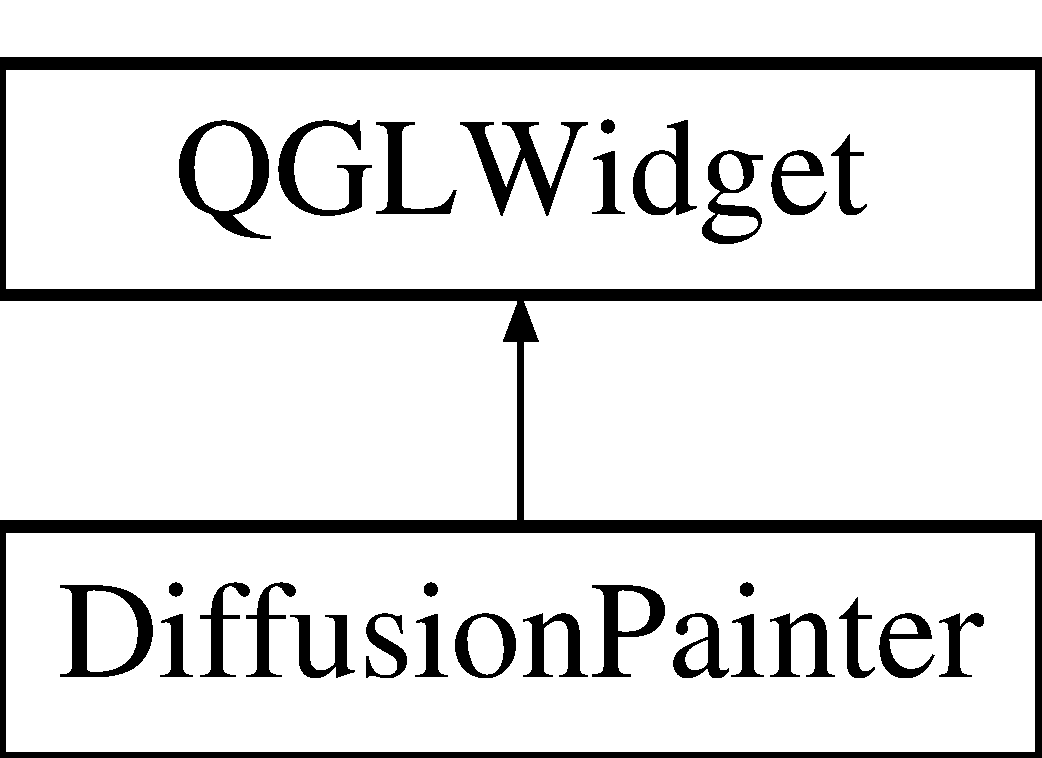
\includegraphics[height=2.000000cm]{class_diffusion_painter}
\end{center}
\end{figure}
\subsection*{Public Slots}
\begin{DoxyCompactItemize}
\item 
void \hyperlink{class_diffusion_painter_a2c914637778dac04b998f66084bf68c2}{set\+X\+Rotation} (int angle)
\begin{DoxyCompactList}\small\item\em \mbox{[}5\mbox{]} \end{DoxyCompactList}\item 
void \hyperlink{class_diffusion_painter_a14bfd44d0c65a6b8a70121a65d25f5fa}{set\+Y\+Rotation} (int angle)
\begin{DoxyCompactList}\small\item\em \mbox{[}5\mbox{]} \end{DoxyCompactList}\item 
void \hyperlink{class_diffusion_painter_a3a33e4601571657252b56fada7ed0a80}{set\+Z\+Rotation} (int angle)
\item 
void \hyperlink{class_diffusion_painter_a45977cebc1e59c5067c00f6179899be5}{set\+Current\+Painter\+\_\+\+Diffusion} ()
\item 
void \hyperlink{class_diffusion_painter_af6c1819f308806fef7583efcc1999f1c}{set\+Current\+Painter\+\_\+\+Selector} ()
\item 
void \hyperlink{class_diffusion_painter_ab7f54b0f193a334bf9e34df65560bffa}{set\+Current\+Painter\+\_\+\+Bezier1} ()
\item 
void \hyperlink{class_diffusion_painter_a8c88f685894a212dad8d1719d8753d2f}{set\+Current\+Painter\+\_\+\+Bezier2} ()
\item 
void \hyperlink{class_diffusion_painter_af00f71174aaa3bb3d7e7c6273d5cacb9}{set\+Current\+Painter\+\_\+\+Anisotrophy} ()
\item 
void \hyperlink{class_diffusion_painter_acf3d7da78c5ffb2b129d951ec80e1bc6}{set\+Sigma} (int value)
\item 
void \hyperlink{class_diffusion_painter_a8d4c6a4de96dae6b77cbf7cf21e0fe59}{set\+Upper\+Limit} (double value)
\item 
void \hyperlink{class_diffusion_painter_a2c1af0a12e7a22b239fa0fa7587babe9}{set\+Lower\+Limit} (double value)
\item 
void \hyperlink{class_diffusion_painter_abaa3b7e44c4494471bc22117661ba51f}{set\+Amplitude} (int value)
\item 
void \hyperlink{class_diffusion_painter_af5b4e33b0f9b840e2c510283d4dba68b}{update\+Canvas} ()
\begin{DoxyCompactList}\small\item\em \mbox{[}10\mbox{]} \end{DoxyCompactList}\end{DoxyCompactItemize}
\subsection*{Signals}
\begin{DoxyCompactItemize}
\item 
void \hyperlink{class_diffusion_painter_a9599253ac2faec4e4fcde0bddc4f2739}{x\+Rotation\+Changed} (int angle)
\item 
void \hyperlink{class_diffusion_painter_a327e74a49eb97c73639588de45ef7cc1}{y\+Rotation\+Changed} (int angle)
\item 
void \hyperlink{class_diffusion_painter_a30c98779110e1e02e9a6d0541a66c5a6}{z\+Rotation\+Changed} (int angle)
\item 
void \hyperlink{class_diffusion_painter_ad5ca1a51002b96b7aae86de9176acb02}{selected\+Node} (int, int)
\item 
void \hyperlink{class_diffusion_painter_a7f0ef90d74b5eb4630164bd350722ac8}{position\+Elektrode} (int, int, int)
\item 
void \hyperlink{class_diffusion_painter_a5ae021b66810c160b95dd4eb3dfd67fb}{emit\+Width} (double)
\item 
void \hyperlink{class_diffusion_painter_abde8585db92da4b64d350d61c827339f}{found\+Point} (int, int)
\end{DoxyCompactItemize}
\subsection*{Public Member Functions}
\begin{DoxyCompactItemize}
\item 
\hyperlink{class_diffusion_painter_a171b9c615611e9f225187f81807c00cf}{Diffusion\+Painter} (\hyperlink{class_cardiac_mesh}{Cardiac\+Mesh} $\ast$grid, \hyperlink{class_diffusion_matrix}{Diffusion\+Matrix} $\ast$pixelmap, \hyperlink{class_diffusion_matrix}{Diffusion\+Matrix} $\ast$anisotrophy, Q\+Widget $\ast$parent=0)
\begin{DoxyCompactList}\small\item\em \mbox{[}0\mbox{]} \end{DoxyCompactList}\item 
\hyperlink{class_diffusion_painter_a4e93ad45e684e622a6923bbf9871d04e}{$\sim$\+Diffusion\+Painter} ()
\item 
void \hyperlink{class_diffusion_painter_a32a09b7f3f568fff71b881ddcb729963}{init\+Painter} (\hyperlink{class_cardiac_mesh}{Cardiac\+Mesh} $\ast$grid, \hyperlink{class_diffusion_matrix}{Diffusion\+Matrix} $\ast$pixelmap)
\item 
void \hyperlink{class_diffusion_painter_a08714d5fcd525bb6a1451229e44e5cb2}{init\+Probes} (int e1\+\_\+x, int e1\+\_\+y, int e2\+\_\+x, int e2\+\_\+y, int e3\+\_\+x, int e3\+\_\+y)
\item 
void \hyperlink{class_diffusion_painter_ab71f8ba7699d9caf7927e21914c6303c}{destroy\+Painter} ()
\item 
Q\+Size \hyperlink{class_diffusion_painter_a37a27acb926fa7963fab1b8fe6763542}{minimum\+Size\+Hint} () const 
\item 
Q\+Size \hyperlink{class_diffusion_painter_a9ce48c2feffb9bcca38227cf930891ff}{size\+Hint} () const 
\begin{DoxyCompactList}\small\item\em \mbox{[}2\mbox{]} \end{DoxyCompactList}\end{DoxyCompactItemize}
\subsection*{Public Attributes}
\begin{DoxyCompactItemize}
\item 
\hyperlink{class_c_camera}{C\+Camera} \hyperlink{class_diffusion_painter_a1e66d5dd4118326a1e1a7bb45efac9f0}{obj\+Camera}
\item 
\hyperlink{class_cardiac_mesh}{Cardiac\+Mesh} $\ast$ \hyperlink{class_diffusion_painter_ad405e9e83988d4e31abc060c7fa53f58}{m\+\_\+grid}
\item 
\hyperlink{class_random_generator}{Random\+Generator} $\ast$ \hyperlink{class_diffusion_painter_a899e223882748c213c482f298ed2cc6a}{rand\+Machine}
\item 
\hyperlink{class_diffusion_matrix}{Diffusion\+Matrix} $\ast$ \hyperlink{class_diffusion_painter_a6a402014322aadca9e82bcf419d9b0c7}{m\+\_\+pixelmap}
\item 
\hyperlink{class_diffusion_matrix}{Diffusion\+Matrix} $\ast$ \hyperlink{class_diffusion_painter_a41a28924c03b3be5a3f7e4bee530345b}{m\+\_\+anisotrophy}
\item 
\hyperlink{class_probe}{Probe} $\ast$ \hyperlink{class_diffusion_painter_aaad25aaf3a5a9bd133a903f4e5afa109}{probe1}
\item 
\hyperlink{class_probe}{Probe} $\ast$ \hyperlink{class_diffusion_painter_a7e1f6b5119f36b87b2f6a6de6df14865}{probe2}
\item 
\hyperlink{class_probe}{Probe} $\ast$ \hyperlink{class_diffusion_painter_a977dd52f37fe18bac0c3c3f33e5aafa4}{probe3}
\item 
bool \hyperlink{class_diffusion_painter_a296bff01cbabce25cdf1f57a3b65b98c}{probe1on}
\item 
bool \hyperlink{class_diffusion_painter_a7a436a62915aff0201b9b5e742ca9a62}{probe2on}
\item 
bool \hyperlink{class_diffusion_painter_ad923bf9dfbf4a10b8231037cf3070831}{probe3on}
\item 
int \hyperlink{class_diffusion_painter_a9ea99ac669bf6661a46ea41dbabc7521}{current\+Moover}
\item 
\hyperlink{class_pix}{Pix} $\ast$ \hyperlink{class_diffusion_painter_aa57b223dd919193fe1ac1b38ddeee4a4}{currently\+Pressed} \mbox{[}3\mbox{]}
\item 
double \hyperlink{class_diffusion_painter_a7884d552b7170c5e9573aa661c16ca44}{m\+\_\+pixel\+Size}
\item 
double \hyperlink{class_diffusion_painter_a09984e636cac8045cb45271593a042c4}{m\+\_\+sigma}
\item 
double \hyperlink{class_diffusion_painter_a7a6623d01ae04592e1aca9d07120d0be}{m\+\_\+amplitude}
\item 
double \hyperlink{class_diffusion_painter_a242c4d131a57f225a9065328f8983e31}{m\+\_\+move\+\_\+diminisher}
\item 
double \hyperlink{class_diffusion_painter_acd61d99ea11dfc944dd587e06aee12f3}{m\+\_\+upper\+Limit}
\item 
double \hyperlink{class_diffusion_painter_a4403369545b46ea79445e7fd71d85616}{m\+\_\+lower\+Limit}
\item 
int \hyperlink{class_diffusion_painter_a30867ab87333582db17ae21e586adc36}{work\+Mode}
\end{DoxyCompactItemize}
\subsection*{Protected Member Functions}
\begin{DoxyCompactItemize}
\item 
void \hyperlink{class_diffusion_painter_a55b1412158c32feaa3449225ab440f61}{initialize\+G\+L} ()
\begin{DoxyCompactList}\small\item\em \mbox{[}1\mbox{]} \end{DoxyCompactList}\item 
void \hyperlink{class_diffusion_painter_a4b876a03a2175a83fdbc5d01cc09adb5}{paint\+G\+L} ()
\begin{DoxyCompactList}\small\item\em \mbox{[}6\mbox{]} \end{DoxyCompactList}\item 
void \hyperlink{class_diffusion_painter_a0d1b9ab8c76b65993e58aae112c05d26}{resize\+G\+L} (int width, int height)
\begin{DoxyCompactList}\small\item\em \mbox{[}7\mbox{]} \end{DoxyCompactList}\item 
void \hyperlink{class_diffusion_painter_aa9ba23c0677c1322a10b7e408790ecca}{mouse\+Press\+Event} (Q\+Mouse\+Event $\ast$event)
\begin{DoxyCompactList}\small\item\em \mbox{[}8\mbox{]} \end{DoxyCompactList}\item 
void \hyperlink{class_diffusion_painter_afc66b6fca1954ad337c7a7b312c48b02}{mouse\+Move\+Event} (Q\+Mouse\+Event $\ast$event)
\end{DoxyCompactItemize}


\subsection{Constructor \& Destructor Documentation}
\hypertarget{class_diffusion_painter_a171b9c615611e9f225187f81807c00cf}{\index{Diffusion\+Painter@{Diffusion\+Painter}!Diffusion\+Painter@{Diffusion\+Painter}}
\index{Diffusion\+Painter@{Diffusion\+Painter}!Diffusion\+Painter@{Diffusion\+Painter}}
\subsubsection[{Diffusion\+Painter}]{\setlength{\rightskip}{0pt plus 5cm}Diffusion\+Painter\+::\+Diffusion\+Painter (
\begin{DoxyParamCaption}
\item[{{\bf Cardiac\+Mesh} $\ast$}]{grid, }
\item[{{\bf Diffusion\+Matrix} $\ast$}]{pixelmap, }
\item[{{\bf Diffusion\+Matrix} $\ast$}]{anisotrophy, }
\item[{Q\+Widget $\ast$}]{parent = {\ttfamily 0}}
\end{DoxyParamCaption}
)}}\label{class_diffusion_painter_a171b9c615611e9f225187f81807c00cf}


\mbox{[}0\mbox{]} 

\hypertarget{class_diffusion_painter_a4e93ad45e684e622a6923bbf9871d04e}{\index{Diffusion\+Painter@{Diffusion\+Painter}!````~Diffusion\+Painter@{$\sim$\+Diffusion\+Painter}}
\index{````~Diffusion\+Painter@{$\sim$\+Diffusion\+Painter}!Diffusion\+Painter@{Diffusion\+Painter}}
\subsubsection[{$\sim$\+Diffusion\+Painter}]{\setlength{\rightskip}{0pt plus 5cm}Diffusion\+Painter\+::$\sim$\+Diffusion\+Painter (
\begin{DoxyParamCaption}
{}
\end{DoxyParamCaption}
)}}\label{class_diffusion_painter_a4e93ad45e684e622a6923bbf9871d04e}


\subsection{Member Function Documentation}
\hypertarget{class_diffusion_painter_ab71f8ba7699d9caf7927e21914c6303c}{\index{Diffusion\+Painter@{Diffusion\+Painter}!destroy\+Painter@{destroy\+Painter}}
\index{destroy\+Painter@{destroy\+Painter}!Diffusion\+Painter@{Diffusion\+Painter}}
\subsubsection[{destroy\+Painter}]{\setlength{\rightskip}{0pt plus 5cm}void Diffusion\+Painter\+::destroy\+Painter (
\begin{DoxyParamCaption}
{}
\end{DoxyParamCaption}
)}}\label{class_diffusion_painter_ab71f8ba7699d9caf7927e21914c6303c}
\hypertarget{class_diffusion_painter_a5ae021b66810c160b95dd4eb3dfd67fb}{\index{Diffusion\+Painter@{Diffusion\+Painter}!emit\+Width@{emit\+Width}}
\index{emit\+Width@{emit\+Width}!Diffusion\+Painter@{Diffusion\+Painter}}
\subsubsection[{emit\+Width}]{\setlength{\rightskip}{0pt plus 5cm}void Diffusion\+Painter\+::emit\+Width (
\begin{DoxyParamCaption}
\item[{double}]{}
\end{DoxyParamCaption}
)\hspace{0.3cm}{\ttfamily [signal]}}}\label{class_diffusion_painter_a5ae021b66810c160b95dd4eb3dfd67fb}
\hypertarget{class_diffusion_painter_abde8585db92da4b64d350d61c827339f}{\index{Diffusion\+Painter@{Diffusion\+Painter}!found\+Point@{found\+Point}}
\index{found\+Point@{found\+Point}!Diffusion\+Painter@{Diffusion\+Painter}}
\subsubsection[{found\+Point}]{\setlength{\rightskip}{0pt plus 5cm}void Diffusion\+Painter\+::found\+Point (
\begin{DoxyParamCaption}
\item[{int}]{, }
\item[{int}]{}
\end{DoxyParamCaption}
)\hspace{0.3cm}{\ttfamily [signal]}}}\label{class_diffusion_painter_abde8585db92da4b64d350d61c827339f}
\hypertarget{class_diffusion_painter_a55b1412158c32feaa3449225ab440f61}{\index{Diffusion\+Painter@{Diffusion\+Painter}!initialize\+G\+L@{initialize\+G\+L}}
\index{initialize\+G\+L@{initialize\+G\+L}!Diffusion\+Painter@{Diffusion\+Painter}}
\subsubsection[{initialize\+G\+L}]{\setlength{\rightskip}{0pt plus 5cm}void Diffusion\+Painter\+::initialize\+G\+L (
\begin{DoxyParamCaption}
{}
\end{DoxyParamCaption}
)\hspace{0.3cm}{\ttfamily [protected]}}}\label{class_diffusion_painter_a55b1412158c32feaa3449225ab440f61}


\mbox{[}1\mbox{]} 

\mbox{[}6\mbox{]}

\mbox{[}2\mbox{]} \hypertarget{class_diffusion_painter_a32a09b7f3f568fff71b881ddcb729963}{\index{Diffusion\+Painter@{Diffusion\+Painter}!init\+Painter@{init\+Painter}}
\index{init\+Painter@{init\+Painter}!Diffusion\+Painter@{Diffusion\+Painter}}
\subsubsection[{init\+Painter}]{\setlength{\rightskip}{0pt plus 5cm}void Diffusion\+Painter\+::init\+Painter (
\begin{DoxyParamCaption}
\item[{{\bf Cardiac\+Mesh} $\ast$}]{grid, }
\item[{{\bf Diffusion\+Matrix} $\ast$}]{pixelmap}
\end{DoxyParamCaption}
)}}\label{class_diffusion_painter_a32a09b7f3f568fff71b881ddcb729963}
\hypertarget{class_diffusion_painter_a08714d5fcd525bb6a1451229e44e5cb2}{\index{Diffusion\+Painter@{Diffusion\+Painter}!init\+Probes@{init\+Probes}}
\index{init\+Probes@{init\+Probes}!Diffusion\+Painter@{Diffusion\+Painter}}
\subsubsection[{init\+Probes}]{\setlength{\rightskip}{0pt plus 5cm}void Diffusion\+Painter\+::init\+Probes (
\begin{DoxyParamCaption}
\item[{int}]{e1\+\_\+x, }
\item[{int}]{e1\+\_\+y, }
\item[{int}]{e2\+\_\+x, }
\item[{int}]{e2\+\_\+y, }
\item[{int}]{e3\+\_\+x, }
\item[{int}]{e3\+\_\+y}
\end{DoxyParamCaption}
)}}\label{class_diffusion_painter_a08714d5fcd525bb6a1451229e44e5cb2}
\hypertarget{class_diffusion_painter_a37a27acb926fa7963fab1b8fe6763542}{\index{Diffusion\+Painter@{Diffusion\+Painter}!minimum\+Size\+Hint@{minimum\+Size\+Hint}}
\index{minimum\+Size\+Hint@{minimum\+Size\+Hint}!Diffusion\+Painter@{Diffusion\+Painter}}
\subsubsection[{minimum\+Size\+Hint}]{\setlength{\rightskip}{0pt plus 5cm}Q\+Size Diffusion\+Painter\+::minimum\+Size\+Hint (
\begin{DoxyParamCaption}
{}
\end{DoxyParamCaption}
) const}}\label{class_diffusion_painter_a37a27acb926fa7963fab1b8fe6763542}
\hypertarget{class_diffusion_painter_afc66b6fca1954ad337c7a7b312c48b02}{\index{Diffusion\+Painter@{Diffusion\+Painter}!mouse\+Move\+Event@{mouse\+Move\+Event}}
\index{mouse\+Move\+Event@{mouse\+Move\+Event}!Diffusion\+Painter@{Diffusion\+Painter}}
\subsubsection[{mouse\+Move\+Event}]{\setlength{\rightskip}{0pt plus 5cm}void Diffusion\+Painter\+::mouse\+Move\+Event (
\begin{DoxyParamCaption}
\item[{Q\+Mouse\+Event $\ast$}]{event}
\end{DoxyParamCaption}
)\hspace{0.3cm}{\ttfamily [protected]}}}\label{class_diffusion_painter_afc66b6fca1954ad337c7a7b312c48b02}
\hypertarget{class_diffusion_painter_aa9ba23c0677c1322a10b7e408790ecca}{\index{Diffusion\+Painter@{Diffusion\+Painter}!mouse\+Press\+Event@{mouse\+Press\+Event}}
\index{mouse\+Press\+Event@{mouse\+Press\+Event}!Diffusion\+Painter@{Diffusion\+Painter}}
\subsubsection[{mouse\+Press\+Event}]{\setlength{\rightskip}{0pt plus 5cm}void Diffusion\+Painter\+::mouse\+Press\+Event (
\begin{DoxyParamCaption}
\item[{Q\+Mouse\+Event $\ast$}]{event}
\end{DoxyParamCaption}
)\hspace{0.3cm}{\ttfamily [protected]}}}\label{class_diffusion_painter_aa9ba23c0677c1322a10b7e408790ecca}


\mbox{[}8\mbox{]} 

\mbox{[}9\mbox{]} \hypertarget{class_diffusion_painter_a4b876a03a2175a83fdbc5d01cc09adb5}{\index{Diffusion\+Painter@{Diffusion\+Painter}!paint\+G\+L@{paint\+G\+L}}
\index{paint\+G\+L@{paint\+G\+L}!Diffusion\+Painter@{Diffusion\+Painter}}
\subsubsection[{paint\+G\+L}]{\setlength{\rightskip}{0pt plus 5cm}void Diffusion\+Painter\+::paint\+G\+L (
\begin{DoxyParamCaption}
{}
\end{DoxyParamCaption}
)\hspace{0.3cm}{\ttfamily [protected]}}}\label{class_diffusion_painter_a4b876a03a2175a83fdbc5d01cc09adb5}


\mbox{[}6\mbox{]} 

\mbox{[}7\mbox{]} \hypertarget{class_diffusion_painter_a7f0ef90d74b5eb4630164bd350722ac8}{\index{Diffusion\+Painter@{Diffusion\+Painter}!position\+Elektrode@{position\+Elektrode}}
\index{position\+Elektrode@{position\+Elektrode}!Diffusion\+Painter@{Diffusion\+Painter}}
\subsubsection[{position\+Elektrode}]{\setlength{\rightskip}{0pt plus 5cm}void Diffusion\+Painter\+::position\+Elektrode (
\begin{DoxyParamCaption}
\item[{int}]{, }
\item[{int}]{, }
\item[{int}]{}
\end{DoxyParamCaption}
)\hspace{0.3cm}{\ttfamily [signal]}}}\label{class_diffusion_painter_a7f0ef90d74b5eb4630164bd350722ac8}
\hypertarget{class_diffusion_painter_a0d1b9ab8c76b65993e58aae112c05d26}{\index{Diffusion\+Painter@{Diffusion\+Painter}!resize\+G\+L@{resize\+G\+L}}
\index{resize\+G\+L@{resize\+G\+L}!Diffusion\+Painter@{Diffusion\+Painter}}
\subsubsection[{resize\+G\+L}]{\setlength{\rightskip}{0pt plus 5cm}void Diffusion\+Painter\+::resize\+G\+L (
\begin{DoxyParamCaption}
\item[{int}]{width, }
\item[{int}]{height}
\end{DoxyParamCaption}
)\hspace{0.3cm}{\ttfamily [protected]}}}\label{class_diffusion_painter_a0d1b9ab8c76b65993e58aae112c05d26}


\mbox{[}7\mbox{]} 

\mbox{[}8\mbox{]} \hypertarget{class_diffusion_painter_ad5ca1a51002b96b7aae86de9176acb02}{\index{Diffusion\+Painter@{Diffusion\+Painter}!selected\+Node@{selected\+Node}}
\index{selected\+Node@{selected\+Node}!Diffusion\+Painter@{Diffusion\+Painter}}
\subsubsection[{selected\+Node}]{\setlength{\rightskip}{0pt plus 5cm}void Diffusion\+Painter\+::selected\+Node (
\begin{DoxyParamCaption}
\item[{int}]{, }
\item[{int}]{}
\end{DoxyParamCaption}
)\hspace{0.3cm}{\ttfamily [signal]}}}\label{class_diffusion_painter_ad5ca1a51002b96b7aae86de9176acb02}
\hypertarget{class_diffusion_painter_abaa3b7e44c4494471bc22117661ba51f}{\index{Diffusion\+Painter@{Diffusion\+Painter}!set\+Amplitude@{set\+Amplitude}}
\index{set\+Amplitude@{set\+Amplitude}!Diffusion\+Painter@{Diffusion\+Painter}}
\subsubsection[{set\+Amplitude}]{\setlength{\rightskip}{0pt plus 5cm}void Diffusion\+Painter\+::set\+Amplitude (
\begin{DoxyParamCaption}
\item[{int}]{value}
\end{DoxyParamCaption}
)\hspace{0.3cm}{\ttfamily [slot]}}}\label{class_diffusion_painter_abaa3b7e44c4494471bc22117661ba51f}
\hypertarget{class_diffusion_painter_af00f71174aaa3bb3d7e7c6273d5cacb9}{\index{Diffusion\+Painter@{Diffusion\+Painter}!set\+Current\+Painter\+\_\+\+Anisotrophy@{set\+Current\+Painter\+\_\+\+Anisotrophy}}
\index{set\+Current\+Painter\+\_\+\+Anisotrophy@{set\+Current\+Painter\+\_\+\+Anisotrophy}!Diffusion\+Painter@{Diffusion\+Painter}}
\subsubsection[{set\+Current\+Painter\+\_\+\+Anisotrophy}]{\setlength{\rightskip}{0pt plus 5cm}void Diffusion\+Painter\+::set\+Current\+Painter\+\_\+\+Anisotrophy (
\begin{DoxyParamCaption}
{}
\end{DoxyParamCaption}
)\hspace{0.3cm}{\ttfamily [slot]}}}\label{class_diffusion_painter_af00f71174aaa3bb3d7e7c6273d5cacb9}
\hypertarget{class_diffusion_painter_ab7f54b0f193a334bf9e34df65560bffa}{\index{Diffusion\+Painter@{Diffusion\+Painter}!set\+Current\+Painter\+\_\+\+Bezier1@{set\+Current\+Painter\+\_\+\+Bezier1}}
\index{set\+Current\+Painter\+\_\+\+Bezier1@{set\+Current\+Painter\+\_\+\+Bezier1}!Diffusion\+Painter@{Diffusion\+Painter}}
\subsubsection[{set\+Current\+Painter\+\_\+\+Bezier1}]{\setlength{\rightskip}{0pt plus 5cm}void Diffusion\+Painter\+::set\+Current\+Painter\+\_\+\+Bezier1 (
\begin{DoxyParamCaption}
{}
\end{DoxyParamCaption}
)\hspace{0.3cm}{\ttfamily [slot]}}}\label{class_diffusion_painter_ab7f54b0f193a334bf9e34df65560bffa}
\hypertarget{class_diffusion_painter_a8c88f685894a212dad8d1719d8753d2f}{\index{Diffusion\+Painter@{Diffusion\+Painter}!set\+Current\+Painter\+\_\+\+Bezier2@{set\+Current\+Painter\+\_\+\+Bezier2}}
\index{set\+Current\+Painter\+\_\+\+Bezier2@{set\+Current\+Painter\+\_\+\+Bezier2}!Diffusion\+Painter@{Diffusion\+Painter}}
\subsubsection[{set\+Current\+Painter\+\_\+\+Bezier2}]{\setlength{\rightskip}{0pt plus 5cm}void Diffusion\+Painter\+::set\+Current\+Painter\+\_\+\+Bezier2 (
\begin{DoxyParamCaption}
{}
\end{DoxyParamCaption}
)\hspace{0.3cm}{\ttfamily [slot]}}}\label{class_diffusion_painter_a8c88f685894a212dad8d1719d8753d2f}
\hypertarget{class_diffusion_painter_a45977cebc1e59c5067c00f6179899be5}{\index{Diffusion\+Painter@{Diffusion\+Painter}!set\+Current\+Painter\+\_\+\+Diffusion@{set\+Current\+Painter\+\_\+\+Diffusion}}
\index{set\+Current\+Painter\+\_\+\+Diffusion@{set\+Current\+Painter\+\_\+\+Diffusion}!Diffusion\+Painter@{Diffusion\+Painter}}
\subsubsection[{set\+Current\+Painter\+\_\+\+Diffusion}]{\setlength{\rightskip}{0pt plus 5cm}void Diffusion\+Painter\+::set\+Current\+Painter\+\_\+\+Diffusion (
\begin{DoxyParamCaption}
{}
\end{DoxyParamCaption}
)\hspace{0.3cm}{\ttfamily [slot]}}}\label{class_diffusion_painter_a45977cebc1e59c5067c00f6179899be5}
\hypertarget{class_diffusion_painter_af6c1819f308806fef7583efcc1999f1c}{\index{Diffusion\+Painter@{Diffusion\+Painter}!set\+Current\+Painter\+\_\+\+Selector@{set\+Current\+Painter\+\_\+\+Selector}}
\index{set\+Current\+Painter\+\_\+\+Selector@{set\+Current\+Painter\+\_\+\+Selector}!Diffusion\+Painter@{Diffusion\+Painter}}
\subsubsection[{set\+Current\+Painter\+\_\+\+Selector}]{\setlength{\rightskip}{0pt plus 5cm}void Diffusion\+Painter\+::set\+Current\+Painter\+\_\+\+Selector (
\begin{DoxyParamCaption}
{}
\end{DoxyParamCaption}
)\hspace{0.3cm}{\ttfamily [slot]}}}\label{class_diffusion_painter_af6c1819f308806fef7583efcc1999f1c}
\hypertarget{class_diffusion_painter_a2c1af0a12e7a22b239fa0fa7587babe9}{\index{Diffusion\+Painter@{Diffusion\+Painter}!set\+Lower\+Limit@{set\+Lower\+Limit}}
\index{set\+Lower\+Limit@{set\+Lower\+Limit}!Diffusion\+Painter@{Diffusion\+Painter}}
\subsubsection[{set\+Lower\+Limit}]{\setlength{\rightskip}{0pt plus 5cm}void Diffusion\+Painter\+::set\+Lower\+Limit (
\begin{DoxyParamCaption}
\item[{double}]{value}
\end{DoxyParamCaption}
)\hspace{0.3cm}{\ttfamily [slot]}}}\label{class_diffusion_painter_a2c1af0a12e7a22b239fa0fa7587babe9}
\hypertarget{class_diffusion_painter_acf3d7da78c5ffb2b129d951ec80e1bc6}{\index{Diffusion\+Painter@{Diffusion\+Painter}!set\+Sigma@{set\+Sigma}}
\index{set\+Sigma@{set\+Sigma}!Diffusion\+Painter@{Diffusion\+Painter}}
\subsubsection[{set\+Sigma}]{\setlength{\rightskip}{0pt plus 5cm}void Diffusion\+Painter\+::set\+Sigma (
\begin{DoxyParamCaption}
\item[{int}]{value}
\end{DoxyParamCaption}
)\hspace{0.3cm}{\ttfamily [slot]}}}\label{class_diffusion_painter_acf3d7da78c5ffb2b129d951ec80e1bc6}
\hypertarget{class_diffusion_painter_a8d4c6a4de96dae6b77cbf7cf21e0fe59}{\index{Diffusion\+Painter@{Diffusion\+Painter}!set\+Upper\+Limit@{set\+Upper\+Limit}}
\index{set\+Upper\+Limit@{set\+Upper\+Limit}!Diffusion\+Painter@{Diffusion\+Painter}}
\subsubsection[{set\+Upper\+Limit}]{\setlength{\rightskip}{0pt plus 5cm}void Diffusion\+Painter\+::set\+Upper\+Limit (
\begin{DoxyParamCaption}
\item[{double}]{value}
\end{DoxyParamCaption}
)\hspace{0.3cm}{\ttfamily [slot]}}}\label{class_diffusion_painter_a8d4c6a4de96dae6b77cbf7cf21e0fe59}
\hypertarget{class_diffusion_painter_a2c914637778dac04b998f66084bf68c2}{\index{Diffusion\+Painter@{Diffusion\+Painter}!set\+X\+Rotation@{set\+X\+Rotation}}
\index{set\+X\+Rotation@{set\+X\+Rotation}!Diffusion\+Painter@{Diffusion\+Painter}}
\subsubsection[{set\+X\+Rotation}]{\setlength{\rightskip}{0pt plus 5cm}void Diffusion\+Painter\+::set\+X\+Rotation (
\begin{DoxyParamCaption}
\item[{int}]{angle}
\end{DoxyParamCaption}
)\hspace{0.3cm}{\ttfamily [slot]}}}\label{class_diffusion_painter_a2c914637778dac04b998f66084bf68c2}


\mbox{[}5\mbox{]} 

\hypertarget{class_diffusion_painter_a14bfd44d0c65a6b8a70121a65d25f5fa}{\index{Diffusion\+Painter@{Diffusion\+Painter}!set\+Y\+Rotation@{set\+Y\+Rotation}}
\index{set\+Y\+Rotation@{set\+Y\+Rotation}!Diffusion\+Painter@{Diffusion\+Painter}}
\subsubsection[{set\+Y\+Rotation}]{\setlength{\rightskip}{0pt plus 5cm}void Diffusion\+Painter\+::set\+Y\+Rotation (
\begin{DoxyParamCaption}
\item[{int}]{angle}
\end{DoxyParamCaption}
)\hspace{0.3cm}{\ttfamily [slot]}}}\label{class_diffusion_painter_a14bfd44d0c65a6b8a70121a65d25f5fa}


\mbox{[}5\mbox{]} 

\hypertarget{class_diffusion_painter_a3a33e4601571657252b56fada7ed0a80}{\index{Diffusion\+Painter@{Diffusion\+Painter}!set\+Z\+Rotation@{set\+Z\+Rotation}}
\index{set\+Z\+Rotation@{set\+Z\+Rotation}!Diffusion\+Painter@{Diffusion\+Painter}}
\subsubsection[{set\+Z\+Rotation}]{\setlength{\rightskip}{0pt plus 5cm}void Diffusion\+Painter\+::set\+Z\+Rotation (
\begin{DoxyParamCaption}
\item[{int}]{angle}
\end{DoxyParamCaption}
)\hspace{0.3cm}{\ttfamily [slot]}}}\label{class_diffusion_painter_a3a33e4601571657252b56fada7ed0a80}
\hypertarget{class_diffusion_painter_a9ce48c2feffb9bcca38227cf930891ff}{\index{Diffusion\+Painter@{Diffusion\+Painter}!size\+Hint@{size\+Hint}}
\index{size\+Hint@{size\+Hint}!Diffusion\+Painter@{Diffusion\+Painter}}
\subsubsection[{size\+Hint}]{\setlength{\rightskip}{0pt plus 5cm}Q\+Size Diffusion\+Painter\+::size\+Hint (
\begin{DoxyParamCaption}
{}
\end{DoxyParamCaption}
) const}}\label{class_diffusion_painter_a9ce48c2feffb9bcca38227cf930891ff}


\mbox{[}2\mbox{]} 

\mbox{[}3\mbox{]} \mbox{[}3\mbox{]} //! \mbox{[}4\mbox{]} \hypertarget{class_diffusion_painter_af5b4e33b0f9b840e2c510283d4dba68b}{\index{Diffusion\+Painter@{Diffusion\+Painter}!update\+Canvas@{update\+Canvas}}
\index{update\+Canvas@{update\+Canvas}!Diffusion\+Painter@{Diffusion\+Painter}}
\subsubsection[{update\+Canvas}]{\setlength{\rightskip}{0pt plus 5cm}void Diffusion\+Painter\+::update\+Canvas (
\begin{DoxyParamCaption}
{}
\end{DoxyParamCaption}
)\hspace{0.3cm}{\ttfamily [slot]}}}\label{class_diffusion_painter_af5b4e33b0f9b840e2c510283d4dba68b}


\mbox{[}10\mbox{]} 

\hypertarget{class_diffusion_painter_a9599253ac2faec4e4fcde0bddc4f2739}{\index{Diffusion\+Painter@{Diffusion\+Painter}!x\+Rotation\+Changed@{x\+Rotation\+Changed}}
\index{x\+Rotation\+Changed@{x\+Rotation\+Changed}!Diffusion\+Painter@{Diffusion\+Painter}}
\subsubsection[{x\+Rotation\+Changed}]{\setlength{\rightskip}{0pt plus 5cm}void Diffusion\+Painter\+::x\+Rotation\+Changed (
\begin{DoxyParamCaption}
\item[{int}]{angle}
\end{DoxyParamCaption}
)\hspace{0.3cm}{\ttfamily [signal]}}}\label{class_diffusion_painter_a9599253ac2faec4e4fcde0bddc4f2739}
\hypertarget{class_diffusion_painter_a327e74a49eb97c73639588de45ef7cc1}{\index{Diffusion\+Painter@{Diffusion\+Painter}!y\+Rotation\+Changed@{y\+Rotation\+Changed}}
\index{y\+Rotation\+Changed@{y\+Rotation\+Changed}!Diffusion\+Painter@{Diffusion\+Painter}}
\subsubsection[{y\+Rotation\+Changed}]{\setlength{\rightskip}{0pt plus 5cm}void Diffusion\+Painter\+::y\+Rotation\+Changed (
\begin{DoxyParamCaption}
\item[{int}]{angle}
\end{DoxyParamCaption}
)\hspace{0.3cm}{\ttfamily [signal]}}}\label{class_diffusion_painter_a327e74a49eb97c73639588de45ef7cc1}
\hypertarget{class_diffusion_painter_a30c98779110e1e02e9a6d0541a66c5a6}{\index{Diffusion\+Painter@{Diffusion\+Painter}!z\+Rotation\+Changed@{z\+Rotation\+Changed}}
\index{z\+Rotation\+Changed@{z\+Rotation\+Changed}!Diffusion\+Painter@{Diffusion\+Painter}}
\subsubsection[{z\+Rotation\+Changed}]{\setlength{\rightskip}{0pt plus 5cm}void Diffusion\+Painter\+::z\+Rotation\+Changed (
\begin{DoxyParamCaption}
\item[{int}]{angle}
\end{DoxyParamCaption}
)\hspace{0.3cm}{\ttfamily [signal]}}}\label{class_diffusion_painter_a30c98779110e1e02e9a6d0541a66c5a6}


\subsection{Member Data Documentation}
\hypertarget{class_diffusion_painter_aa57b223dd919193fe1ac1b38ddeee4a4}{\index{Diffusion\+Painter@{Diffusion\+Painter}!currently\+Pressed@{currently\+Pressed}}
\index{currently\+Pressed@{currently\+Pressed}!Diffusion\+Painter@{Diffusion\+Painter}}
\subsubsection[{currently\+Pressed}]{\setlength{\rightskip}{0pt plus 5cm}{\bf Pix}$\ast$ Diffusion\+Painter\+::currently\+Pressed\mbox{[}3\mbox{]}}}\label{class_diffusion_painter_aa57b223dd919193fe1ac1b38ddeee4a4}
\hypertarget{class_diffusion_painter_a9ea99ac669bf6661a46ea41dbabc7521}{\index{Diffusion\+Painter@{Diffusion\+Painter}!current\+Moover@{current\+Moover}}
\index{current\+Moover@{current\+Moover}!Diffusion\+Painter@{Diffusion\+Painter}}
\subsubsection[{current\+Moover}]{\setlength{\rightskip}{0pt plus 5cm}int Diffusion\+Painter\+::current\+Moover}}\label{class_diffusion_painter_a9ea99ac669bf6661a46ea41dbabc7521}
\hypertarget{class_diffusion_painter_a7a6623d01ae04592e1aca9d07120d0be}{\index{Diffusion\+Painter@{Diffusion\+Painter}!m\+\_\+amplitude@{m\+\_\+amplitude}}
\index{m\+\_\+amplitude@{m\+\_\+amplitude}!Diffusion\+Painter@{Diffusion\+Painter}}
\subsubsection[{m\+\_\+amplitude}]{\setlength{\rightskip}{0pt plus 5cm}double Diffusion\+Painter\+::m\+\_\+amplitude}}\label{class_diffusion_painter_a7a6623d01ae04592e1aca9d07120d0be}
\hypertarget{class_diffusion_painter_a41a28924c03b3be5a3f7e4bee530345b}{\index{Diffusion\+Painter@{Diffusion\+Painter}!m\+\_\+anisotrophy@{m\+\_\+anisotrophy}}
\index{m\+\_\+anisotrophy@{m\+\_\+anisotrophy}!Diffusion\+Painter@{Diffusion\+Painter}}
\subsubsection[{m\+\_\+anisotrophy}]{\setlength{\rightskip}{0pt plus 5cm}{\bf Diffusion\+Matrix}$\ast$ Diffusion\+Painter\+::m\+\_\+anisotrophy}}\label{class_diffusion_painter_a41a28924c03b3be5a3f7e4bee530345b}
\hypertarget{class_diffusion_painter_ad405e9e83988d4e31abc060c7fa53f58}{\index{Diffusion\+Painter@{Diffusion\+Painter}!m\+\_\+grid@{m\+\_\+grid}}
\index{m\+\_\+grid@{m\+\_\+grid}!Diffusion\+Painter@{Diffusion\+Painter}}
\subsubsection[{m\+\_\+grid}]{\setlength{\rightskip}{0pt plus 5cm}{\bf Cardiac\+Mesh}$\ast$ Diffusion\+Painter\+::m\+\_\+grid}}\label{class_diffusion_painter_ad405e9e83988d4e31abc060c7fa53f58}
\hypertarget{class_diffusion_painter_a4403369545b46ea79445e7fd71d85616}{\index{Diffusion\+Painter@{Diffusion\+Painter}!m\+\_\+lower\+Limit@{m\+\_\+lower\+Limit}}
\index{m\+\_\+lower\+Limit@{m\+\_\+lower\+Limit}!Diffusion\+Painter@{Diffusion\+Painter}}
\subsubsection[{m\+\_\+lower\+Limit}]{\setlength{\rightskip}{0pt plus 5cm}double Diffusion\+Painter\+::m\+\_\+lower\+Limit}}\label{class_diffusion_painter_a4403369545b46ea79445e7fd71d85616}
\hypertarget{class_diffusion_painter_a242c4d131a57f225a9065328f8983e31}{\index{Diffusion\+Painter@{Diffusion\+Painter}!m\+\_\+move\+\_\+diminisher@{m\+\_\+move\+\_\+diminisher}}
\index{m\+\_\+move\+\_\+diminisher@{m\+\_\+move\+\_\+diminisher}!Diffusion\+Painter@{Diffusion\+Painter}}
\subsubsection[{m\+\_\+move\+\_\+diminisher}]{\setlength{\rightskip}{0pt plus 5cm}double Diffusion\+Painter\+::m\+\_\+move\+\_\+diminisher}}\label{class_diffusion_painter_a242c4d131a57f225a9065328f8983e31}
\hypertarget{class_diffusion_painter_a6a402014322aadca9e82bcf419d9b0c7}{\index{Diffusion\+Painter@{Diffusion\+Painter}!m\+\_\+pixelmap@{m\+\_\+pixelmap}}
\index{m\+\_\+pixelmap@{m\+\_\+pixelmap}!Diffusion\+Painter@{Diffusion\+Painter}}
\subsubsection[{m\+\_\+pixelmap}]{\setlength{\rightskip}{0pt plus 5cm}{\bf Diffusion\+Matrix}$\ast$ Diffusion\+Painter\+::m\+\_\+pixelmap}}\label{class_diffusion_painter_a6a402014322aadca9e82bcf419d9b0c7}
\hypertarget{class_diffusion_painter_a7884d552b7170c5e9573aa661c16ca44}{\index{Diffusion\+Painter@{Diffusion\+Painter}!m\+\_\+pixel\+Size@{m\+\_\+pixel\+Size}}
\index{m\+\_\+pixel\+Size@{m\+\_\+pixel\+Size}!Diffusion\+Painter@{Diffusion\+Painter}}
\subsubsection[{m\+\_\+pixel\+Size}]{\setlength{\rightskip}{0pt plus 5cm}double Diffusion\+Painter\+::m\+\_\+pixel\+Size}}\label{class_diffusion_painter_a7884d552b7170c5e9573aa661c16ca44}
\hypertarget{class_diffusion_painter_a09984e636cac8045cb45271593a042c4}{\index{Diffusion\+Painter@{Diffusion\+Painter}!m\+\_\+sigma@{m\+\_\+sigma}}
\index{m\+\_\+sigma@{m\+\_\+sigma}!Diffusion\+Painter@{Diffusion\+Painter}}
\subsubsection[{m\+\_\+sigma}]{\setlength{\rightskip}{0pt plus 5cm}double Diffusion\+Painter\+::m\+\_\+sigma}}\label{class_diffusion_painter_a09984e636cac8045cb45271593a042c4}
\hypertarget{class_diffusion_painter_acd61d99ea11dfc944dd587e06aee12f3}{\index{Diffusion\+Painter@{Diffusion\+Painter}!m\+\_\+upper\+Limit@{m\+\_\+upper\+Limit}}
\index{m\+\_\+upper\+Limit@{m\+\_\+upper\+Limit}!Diffusion\+Painter@{Diffusion\+Painter}}
\subsubsection[{m\+\_\+upper\+Limit}]{\setlength{\rightskip}{0pt plus 5cm}double Diffusion\+Painter\+::m\+\_\+upper\+Limit}}\label{class_diffusion_painter_acd61d99ea11dfc944dd587e06aee12f3}
\hypertarget{class_diffusion_painter_a1e66d5dd4118326a1e1a7bb45efac9f0}{\index{Diffusion\+Painter@{Diffusion\+Painter}!obj\+Camera@{obj\+Camera}}
\index{obj\+Camera@{obj\+Camera}!Diffusion\+Painter@{Diffusion\+Painter}}
\subsubsection[{obj\+Camera}]{\setlength{\rightskip}{0pt plus 5cm}{\bf C\+Camera} Diffusion\+Painter\+::obj\+Camera}}\label{class_diffusion_painter_a1e66d5dd4118326a1e1a7bb45efac9f0}
\hypertarget{class_diffusion_painter_aaad25aaf3a5a9bd133a903f4e5afa109}{\index{Diffusion\+Painter@{Diffusion\+Painter}!probe1@{probe1}}
\index{probe1@{probe1}!Diffusion\+Painter@{Diffusion\+Painter}}
\subsubsection[{probe1}]{\setlength{\rightskip}{0pt plus 5cm}{\bf Probe}$\ast$ Diffusion\+Painter\+::probe1}}\label{class_diffusion_painter_aaad25aaf3a5a9bd133a903f4e5afa109}
\hypertarget{class_diffusion_painter_a296bff01cbabce25cdf1f57a3b65b98c}{\index{Diffusion\+Painter@{Diffusion\+Painter}!probe1on@{probe1on}}
\index{probe1on@{probe1on}!Diffusion\+Painter@{Diffusion\+Painter}}
\subsubsection[{probe1on}]{\setlength{\rightskip}{0pt plus 5cm}bool Diffusion\+Painter\+::probe1on}}\label{class_diffusion_painter_a296bff01cbabce25cdf1f57a3b65b98c}
\hypertarget{class_diffusion_painter_a7e1f6b5119f36b87b2f6a6de6df14865}{\index{Diffusion\+Painter@{Diffusion\+Painter}!probe2@{probe2}}
\index{probe2@{probe2}!Diffusion\+Painter@{Diffusion\+Painter}}
\subsubsection[{probe2}]{\setlength{\rightskip}{0pt plus 5cm}{\bf Probe}$\ast$ Diffusion\+Painter\+::probe2}}\label{class_diffusion_painter_a7e1f6b5119f36b87b2f6a6de6df14865}
\hypertarget{class_diffusion_painter_a7a436a62915aff0201b9b5e742ca9a62}{\index{Diffusion\+Painter@{Diffusion\+Painter}!probe2on@{probe2on}}
\index{probe2on@{probe2on}!Diffusion\+Painter@{Diffusion\+Painter}}
\subsubsection[{probe2on}]{\setlength{\rightskip}{0pt plus 5cm}bool Diffusion\+Painter\+::probe2on}}\label{class_diffusion_painter_a7a436a62915aff0201b9b5e742ca9a62}
\hypertarget{class_diffusion_painter_a977dd52f37fe18bac0c3c3f33e5aafa4}{\index{Diffusion\+Painter@{Diffusion\+Painter}!probe3@{probe3}}
\index{probe3@{probe3}!Diffusion\+Painter@{Diffusion\+Painter}}
\subsubsection[{probe3}]{\setlength{\rightskip}{0pt plus 5cm}{\bf Probe}$\ast$ Diffusion\+Painter\+::probe3}}\label{class_diffusion_painter_a977dd52f37fe18bac0c3c3f33e5aafa4}
\hypertarget{class_diffusion_painter_ad923bf9dfbf4a10b8231037cf3070831}{\index{Diffusion\+Painter@{Diffusion\+Painter}!probe3on@{probe3on}}
\index{probe3on@{probe3on}!Diffusion\+Painter@{Diffusion\+Painter}}
\subsubsection[{probe3on}]{\setlength{\rightskip}{0pt plus 5cm}bool Diffusion\+Painter\+::probe3on}}\label{class_diffusion_painter_ad923bf9dfbf4a10b8231037cf3070831}
\hypertarget{class_diffusion_painter_a899e223882748c213c482f298ed2cc6a}{\index{Diffusion\+Painter@{Diffusion\+Painter}!rand\+Machine@{rand\+Machine}}
\index{rand\+Machine@{rand\+Machine}!Diffusion\+Painter@{Diffusion\+Painter}}
\subsubsection[{rand\+Machine}]{\setlength{\rightskip}{0pt plus 5cm}{\bf Random\+Generator}$\ast$ Diffusion\+Painter\+::rand\+Machine}}\label{class_diffusion_painter_a899e223882748c213c482f298ed2cc6a}
\hypertarget{class_diffusion_painter_a30867ab87333582db17ae21e586adc36}{\index{Diffusion\+Painter@{Diffusion\+Painter}!work\+Mode@{work\+Mode}}
\index{work\+Mode@{work\+Mode}!Diffusion\+Painter@{Diffusion\+Painter}}
\subsubsection[{work\+Mode}]{\setlength{\rightskip}{0pt plus 5cm}int Diffusion\+Painter\+::work\+Mode}}\label{class_diffusion_painter_a30867ab87333582db17ae21e586adc36}


The documentation for this class was generated from the following files\+:\begin{DoxyCompactItemize}
\item 
\hyperlink{_diffusion_painter_8h}{Diffusion\+Painter.\+h}\item 
\hyperlink{_diffusion_painter_8cpp}{Diffusion\+Painter.\+cpp}\end{DoxyCompactItemize}

\hypertarget{class_fitz_hugh_nagumo}{\section{Fitz\+Hugh\+Nagumo Class Reference}
\label{class_fitz_hugh_nagumo}\index{Fitz\+Hugh\+Nagumo@{Fitz\+Hugh\+Nagumo}}
}


{\ttfamily \#include $<$Fitz\+Hugh\+Nagumo.\+h$>$}

Inheritance diagram for Fitz\+Hugh\+Nagumo\+:\begin{figure}[H]
\begin{center}
\leavevmode
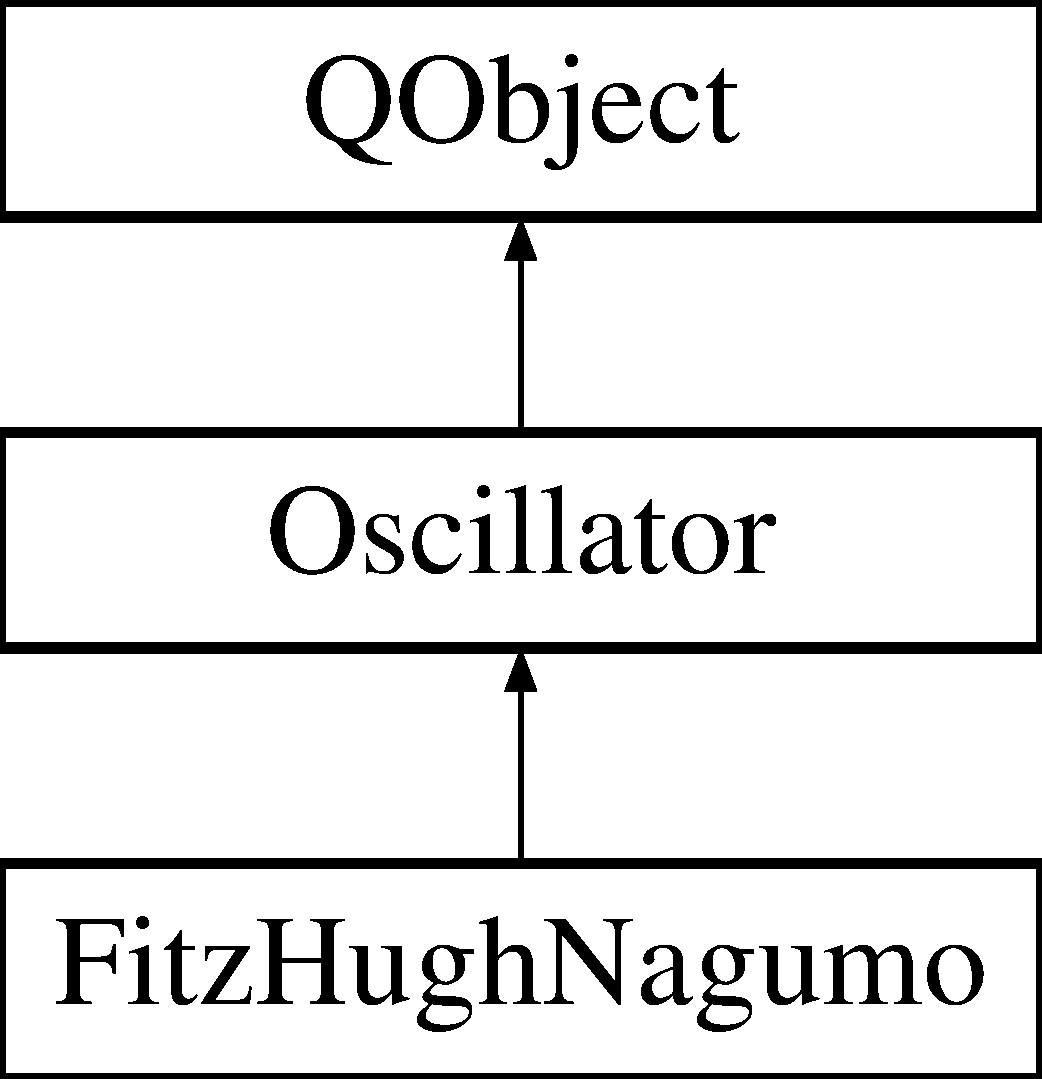
\includegraphics[height=3.000000cm]{class_fitz_hugh_nagumo}
\end{center}
\end{figure}
\subsection*{Public Slots}
\begin{DoxyCompactItemize}
\item 
void \hyperlink{class_fitz_hugh_nagumo_ab1f3c9104230b052ec30096d11dd23b0}{set\+Parameter} (double value, \hyperlink{heart_defines_8h_a79395aba577c2bc57e7ca211ff3476a6}{O\+S\+C\+\_\+\+P\+A\+R\+A\+M\+E\+T\+E\+R} parameter)
\item 
void \hyperlink{class_fitz_hugh_nagumo_a9db9c3133f8f1e3d92f98fc0b1554dac}{set\+Value\+Beta} (double value)
\item 
void \hyperlink{class_fitz_hugh_nagumo_a07d74fdae4fc391eb5d8a3aca7088746}{set\+Value\+Ni} (double value)
\item 
void \hyperlink{class_fitz_hugh_nagumo_a10c8d7c96fe39b0a2b7151092776f6f2}{set\+Value\+Gamma} (double value)
\item 
void \hyperlink{class_fitz_hugh_nagumo_ac1f73cfe6263e8561dc1ddae91819e38}{set\+Default\+Av\+Parameters} ()
\end{DoxyCompactItemize}
\subsection*{Public Member Functions}
\begin{DoxyCompactItemize}
\item 
\hyperlink{class_fitz_hugh_nagumo_a2c8d3d7f70371091eadeab6ce0873404}{Fitz\+Hugh\+Nagumo} (void)
\item 
\hyperlink{class_fitz_hugh_nagumo_a1bc8c62851f3b2306b403ea65f9034ca}{$\sim$\+Fitz\+Hugh\+Nagumo} (void)
\item 
double \hyperlink{class_fitz_hugh_nagumo_a2d09bc9358d92d29c3c403af7f4b33d8}{get\+Current\+Prim} (int which)
\item 
double \hyperlink{class_fitz_hugh_nagumo_ae4d4e8c1c3b9905a0e6aaa5ae0c2f2ed}{get\+Potential\+Prim} ()
\end{DoxyCompactItemize}
\subsection*{Additional Inherited Members}


\subsection{Constructor \& Destructor Documentation}
\hypertarget{class_fitz_hugh_nagumo_a2c8d3d7f70371091eadeab6ce0873404}{\index{Fitz\+Hugh\+Nagumo@{Fitz\+Hugh\+Nagumo}!Fitz\+Hugh\+Nagumo@{Fitz\+Hugh\+Nagumo}}
\index{Fitz\+Hugh\+Nagumo@{Fitz\+Hugh\+Nagumo}!Fitz\+Hugh\+Nagumo@{Fitz\+Hugh\+Nagumo}}
\subsubsection[{Fitz\+Hugh\+Nagumo}]{\setlength{\rightskip}{0pt plus 5cm}Fitz\+Hugh\+Nagumo\+::\+Fitz\+Hugh\+Nagumo (
\begin{DoxyParamCaption}
\item[{void}]{}
\end{DoxyParamCaption}
)}}\label{class_fitz_hugh_nagumo_a2c8d3d7f70371091eadeab6ce0873404}
\hypertarget{class_fitz_hugh_nagumo_a1bc8c62851f3b2306b403ea65f9034ca}{\index{Fitz\+Hugh\+Nagumo@{Fitz\+Hugh\+Nagumo}!````~Fitz\+Hugh\+Nagumo@{$\sim$\+Fitz\+Hugh\+Nagumo}}
\index{````~Fitz\+Hugh\+Nagumo@{$\sim$\+Fitz\+Hugh\+Nagumo}!Fitz\+Hugh\+Nagumo@{Fitz\+Hugh\+Nagumo}}
\subsubsection[{$\sim$\+Fitz\+Hugh\+Nagumo}]{\setlength{\rightskip}{0pt plus 5cm}Fitz\+Hugh\+Nagumo\+::$\sim$\+Fitz\+Hugh\+Nagumo (
\begin{DoxyParamCaption}
\item[{void}]{}
\end{DoxyParamCaption}
)}}\label{class_fitz_hugh_nagumo_a1bc8c62851f3b2306b403ea65f9034ca}


\subsection{Member Function Documentation}
\hypertarget{class_fitz_hugh_nagumo_a2d09bc9358d92d29c3c403af7f4b33d8}{\index{Fitz\+Hugh\+Nagumo@{Fitz\+Hugh\+Nagumo}!get\+Current\+Prim@{get\+Current\+Prim}}
\index{get\+Current\+Prim@{get\+Current\+Prim}!Fitz\+Hugh\+Nagumo@{Fitz\+Hugh\+Nagumo}}
\subsubsection[{get\+Current\+Prim}]{\setlength{\rightskip}{0pt plus 5cm}double Fitz\+Hugh\+Nagumo\+::get\+Current\+Prim (
\begin{DoxyParamCaption}
\item[{int}]{which}
\end{DoxyParamCaption}
)}}\label{class_fitz_hugh_nagumo_a2d09bc9358d92d29c3c403af7f4b33d8}
\hypertarget{class_fitz_hugh_nagumo_ae4d4e8c1c3b9905a0e6aaa5ae0c2f2ed}{\index{Fitz\+Hugh\+Nagumo@{Fitz\+Hugh\+Nagumo}!get\+Potential\+Prim@{get\+Potential\+Prim}}
\index{get\+Potential\+Prim@{get\+Potential\+Prim}!Fitz\+Hugh\+Nagumo@{Fitz\+Hugh\+Nagumo}}
\subsubsection[{get\+Potential\+Prim}]{\setlength{\rightskip}{0pt plus 5cm}double Fitz\+Hugh\+Nagumo\+::get\+Potential\+Prim (
\begin{DoxyParamCaption}
{}
\end{DoxyParamCaption}
)\hspace{0.3cm}{\ttfamily [virtual]}}}\label{class_fitz_hugh_nagumo_ae4d4e8c1c3b9905a0e6aaa5ae0c2f2ed}


Reimplemented from \hyperlink{class_oscillator_a932fda2705d851fbe28c569547f4b4f1}{Oscillator}.

\hypertarget{class_fitz_hugh_nagumo_ac1f73cfe6263e8561dc1ddae91819e38}{\index{Fitz\+Hugh\+Nagumo@{Fitz\+Hugh\+Nagumo}!set\+Default\+Av\+Parameters@{set\+Default\+Av\+Parameters}}
\index{set\+Default\+Av\+Parameters@{set\+Default\+Av\+Parameters}!Fitz\+Hugh\+Nagumo@{Fitz\+Hugh\+Nagumo}}
\subsubsection[{set\+Default\+Av\+Parameters}]{\setlength{\rightskip}{0pt plus 5cm}void Fitz\+Hugh\+Nagumo\+::set\+Default\+Av\+Parameters (
\begin{DoxyParamCaption}
{}
\end{DoxyParamCaption}
)\hspace{0.3cm}{\ttfamily [slot]}}}\label{class_fitz_hugh_nagumo_ac1f73cfe6263e8561dc1ddae91819e38}
\hypertarget{class_fitz_hugh_nagumo_ab1f3c9104230b052ec30096d11dd23b0}{\index{Fitz\+Hugh\+Nagumo@{Fitz\+Hugh\+Nagumo}!set\+Parameter@{set\+Parameter}}
\index{set\+Parameter@{set\+Parameter}!Fitz\+Hugh\+Nagumo@{Fitz\+Hugh\+Nagumo}}
\subsubsection[{set\+Parameter}]{\setlength{\rightskip}{0pt plus 5cm}void Fitz\+Hugh\+Nagumo\+::set\+Parameter (
\begin{DoxyParamCaption}
\item[{double}]{value, }
\item[{{\bf O\+S\+C\+\_\+\+P\+A\+R\+A\+M\+E\+T\+E\+R}}]{parameter}
\end{DoxyParamCaption}
)\hspace{0.3cm}{\ttfamily [slot]}}}\label{class_fitz_hugh_nagumo_ab1f3c9104230b052ec30096d11dd23b0}
\hypertarget{class_fitz_hugh_nagumo_a9db9c3133f8f1e3d92f98fc0b1554dac}{\index{Fitz\+Hugh\+Nagumo@{Fitz\+Hugh\+Nagumo}!set\+Value\+Beta@{set\+Value\+Beta}}
\index{set\+Value\+Beta@{set\+Value\+Beta}!Fitz\+Hugh\+Nagumo@{Fitz\+Hugh\+Nagumo}}
\subsubsection[{set\+Value\+Beta}]{\setlength{\rightskip}{0pt plus 5cm}void Fitz\+Hugh\+Nagumo\+::set\+Value\+Beta (
\begin{DoxyParamCaption}
\item[{double}]{value}
\end{DoxyParamCaption}
)\hspace{0.3cm}{\ttfamily [slot]}}}\label{class_fitz_hugh_nagumo_a9db9c3133f8f1e3d92f98fc0b1554dac}
\hypertarget{class_fitz_hugh_nagumo_a10c8d7c96fe39b0a2b7151092776f6f2}{\index{Fitz\+Hugh\+Nagumo@{Fitz\+Hugh\+Nagumo}!set\+Value\+Gamma@{set\+Value\+Gamma}}
\index{set\+Value\+Gamma@{set\+Value\+Gamma}!Fitz\+Hugh\+Nagumo@{Fitz\+Hugh\+Nagumo}}
\subsubsection[{set\+Value\+Gamma}]{\setlength{\rightskip}{0pt plus 5cm}void Fitz\+Hugh\+Nagumo\+::set\+Value\+Gamma (
\begin{DoxyParamCaption}
\item[{double}]{value}
\end{DoxyParamCaption}
)\hspace{0.3cm}{\ttfamily [slot]}}}\label{class_fitz_hugh_nagumo_a10c8d7c96fe39b0a2b7151092776f6f2}
\hypertarget{class_fitz_hugh_nagumo_a07d74fdae4fc391eb5d8a3aca7088746}{\index{Fitz\+Hugh\+Nagumo@{Fitz\+Hugh\+Nagumo}!set\+Value\+Ni@{set\+Value\+Ni}}
\index{set\+Value\+Ni@{set\+Value\+Ni}!Fitz\+Hugh\+Nagumo@{Fitz\+Hugh\+Nagumo}}
\subsubsection[{set\+Value\+Ni}]{\setlength{\rightskip}{0pt plus 5cm}void Fitz\+Hugh\+Nagumo\+::set\+Value\+Ni (
\begin{DoxyParamCaption}
\item[{double}]{value}
\end{DoxyParamCaption}
)\hspace{0.3cm}{\ttfamily [slot]}}}\label{class_fitz_hugh_nagumo_a07d74fdae4fc391eb5d8a3aca7088746}


The documentation for this class was generated from the following files\+:\begin{DoxyCompactItemize}
\item 
Model/\hyperlink{_fitz_hugh_nagumo_8h}{Fitz\+Hugh\+Nagumo.\+h}\item 
Model/\hyperlink{_fitz_hugh_nagumo_8cpp}{Fitz\+Hugh\+Nagumo.\+cpp}\end{DoxyCompactItemize}

\hypertarget{class_forward_euler_strategy}{\section{Forward\+Euler\+Strategy Class Reference}
\label{class_forward_euler_strategy}\index{Forward\+Euler\+Strategy@{Forward\+Euler\+Strategy}}
}


{\ttfamily \#include $<$Forward\+Euler\+Strategy.\+h$>$}

Inheritance diagram for Forward\+Euler\+Strategy\+:\begin{figure}[H]
\begin{center}
\leavevmode
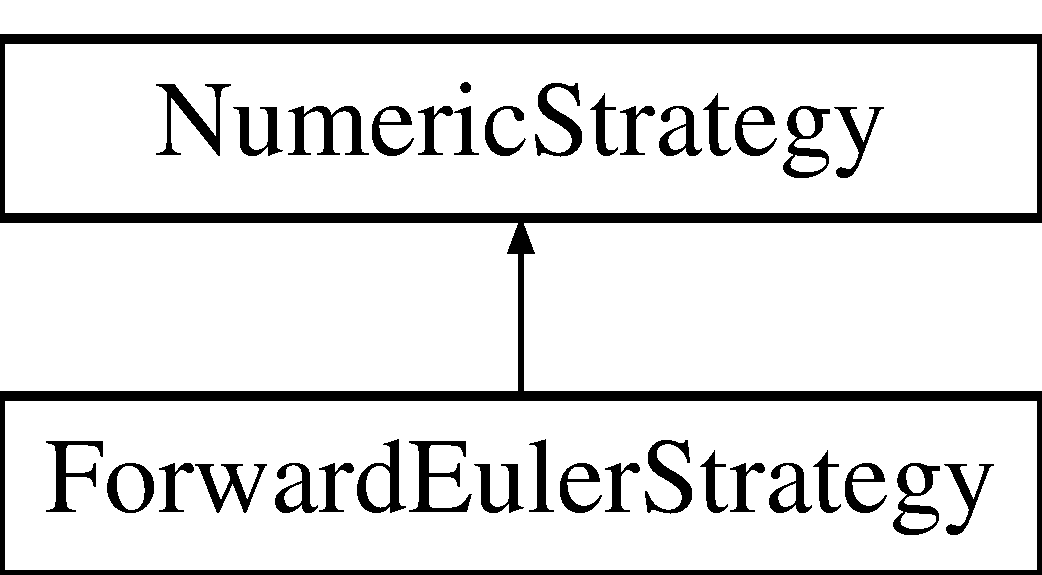
\includegraphics[height=2.000000cm]{class_forward_euler_strategy}
\end{center}
\end{figure}
\subsection*{Public Member Functions}
\begin{DoxyCompactItemize}
\item 
\hyperlink{class_forward_euler_strategy_a34072c0f458fb7946733717cf05956a4}{Forward\+Euler\+Strategy} (\hyperlink{class_cardiac_mesh}{Cardiac\+Mesh} $\ast$oscillators)
\item 
\hyperlink{class_forward_euler_strategy_a2c712bdc098b10499d8033b14302526c}{$\sim$\+Forward\+Euler\+Strategy} ()
\item 
double \hyperlink{class_forward_euler_strategy_a3a382585c2d87ffaf370c07c37737a28}{next\+Step} ()
\begin{DoxyCompactList}\small\item\em Main function. \end{DoxyCompactList}\item 
void \hyperlink{class_forward_euler_strategy_aedd8186805189522eebfafce55617bb9}{reset} ()
\end{DoxyCompactItemize}
\subsection*{Public Attributes}
\begin{DoxyCompactItemize}
\item 
double \hyperlink{class_forward_euler_strategy_aa7cb67aa11fb16d4a76c1944ad3dbbc4}{m\+\_\+main\+Timestep}
\end{DoxyCompactItemize}


\subsection{Constructor \& Destructor Documentation}
\hypertarget{class_forward_euler_strategy_a34072c0f458fb7946733717cf05956a4}{\index{Forward\+Euler\+Strategy@{Forward\+Euler\+Strategy}!Forward\+Euler\+Strategy@{Forward\+Euler\+Strategy}}
\index{Forward\+Euler\+Strategy@{Forward\+Euler\+Strategy}!Forward\+Euler\+Strategy@{Forward\+Euler\+Strategy}}
\subsubsection[{Forward\+Euler\+Strategy}]{\setlength{\rightskip}{0pt plus 5cm}Forward\+Euler\+Strategy\+::\+Forward\+Euler\+Strategy (
\begin{DoxyParamCaption}
\item[{{\bf Cardiac\+Mesh} $\ast$}]{oscillators}
\end{DoxyParamCaption}
)}}\label{class_forward_euler_strategy_a34072c0f458fb7946733717cf05956a4}
\hypertarget{class_forward_euler_strategy_a2c712bdc098b10499d8033b14302526c}{\index{Forward\+Euler\+Strategy@{Forward\+Euler\+Strategy}!````~Forward\+Euler\+Strategy@{$\sim$\+Forward\+Euler\+Strategy}}
\index{````~Forward\+Euler\+Strategy@{$\sim$\+Forward\+Euler\+Strategy}!Forward\+Euler\+Strategy@{Forward\+Euler\+Strategy}}
\subsubsection[{$\sim$\+Forward\+Euler\+Strategy}]{\setlength{\rightskip}{0pt plus 5cm}Forward\+Euler\+Strategy\+::$\sim$\+Forward\+Euler\+Strategy (
\begin{DoxyParamCaption}
{}
\end{DoxyParamCaption}
)}}\label{class_forward_euler_strategy_a2c712bdc098b10499d8033b14302526c}


\subsection{Member Function Documentation}
\hypertarget{class_forward_euler_strategy_a3a382585c2d87ffaf370c07c37737a28}{\index{Forward\+Euler\+Strategy@{Forward\+Euler\+Strategy}!next\+Step@{next\+Step}}
\index{next\+Step@{next\+Step}!Forward\+Euler\+Strategy@{Forward\+Euler\+Strategy}}
\subsubsection[{next\+Step}]{\setlength{\rightskip}{0pt plus 5cm}double Forward\+Euler\+Strategy\+::next\+Step (
\begin{DoxyParamCaption}
{}
\end{DoxyParamCaption}
)\hspace{0.3cm}{\ttfamily [virtual]}}}\label{class_forward_euler_strategy_a3a382585c2d87ffaf370c07c37737a28}


Main function. 



Implements \hyperlink{class_numeric_strategy_aeab387274e9d0ebf46a0e5ad5a5fe73f}{Numeric\+Strategy}.

\hypertarget{class_forward_euler_strategy_aedd8186805189522eebfafce55617bb9}{\index{Forward\+Euler\+Strategy@{Forward\+Euler\+Strategy}!reset@{reset}}
\index{reset@{reset}!Forward\+Euler\+Strategy@{Forward\+Euler\+Strategy}}
\subsubsection[{reset}]{\setlength{\rightskip}{0pt plus 5cm}void Forward\+Euler\+Strategy\+::reset (
\begin{DoxyParamCaption}
{}
\end{DoxyParamCaption}
)\hspace{0.3cm}{\ttfamily [virtual]}}}\label{class_forward_euler_strategy_aedd8186805189522eebfafce55617bb9}


Implements \hyperlink{class_numeric_strategy_a81a1a510394e88edc2705e565d30f017}{Numeric\+Strategy}.



\subsection{Member Data Documentation}
\hypertarget{class_forward_euler_strategy_aa7cb67aa11fb16d4a76c1944ad3dbbc4}{\index{Forward\+Euler\+Strategy@{Forward\+Euler\+Strategy}!m\+\_\+main\+Timestep@{m\+\_\+main\+Timestep}}
\index{m\+\_\+main\+Timestep@{m\+\_\+main\+Timestep}!Forward\+Euler\+Strategy@{Forward\+Euler\+Strategy}}
\subsubsection[{m\+\_\+main\+Timestep}]{\setlength{\rightskip}{0pt plus 5cm}double Forward\+Euler\+Strategy\+::m\+\_\+main\+Timestep}}\label{class_forward_euler_strategy_aa7cb67aa11fb16d4a76c1944ad3dbbc4}


The documentation for this class was generated from the following files\+:\begin{DoxyCompactItemize}
\item 
Numeric\+Strategy/\hyperlink{_forward_euler_strategy_8h}{Forward\+Euler\+Strategy.\+h}\item 
Numeric\+Strategy/\hyperlink{_forward_euler_strategy_8cpp}{Forward\+Euler\+Strategy.\+cpp}\end{DoxyCompactItemize}

\hypertarget{classgl_atrium}{\section{gl\+Atrium Class Reference}
\label{classgl_atrium}\index{gl\+Atrium@{gl\+Atrium}}
}


T\+O\+D\+O Update to Open\+G\+L 3.\+0.  




{\ttfamily \#include $<$gl\+Atrium.\+h$>$}

Inheritance diagram for gl\+Atrium\+:\begin{figure}[H]
\begin{center}
\leavevmode
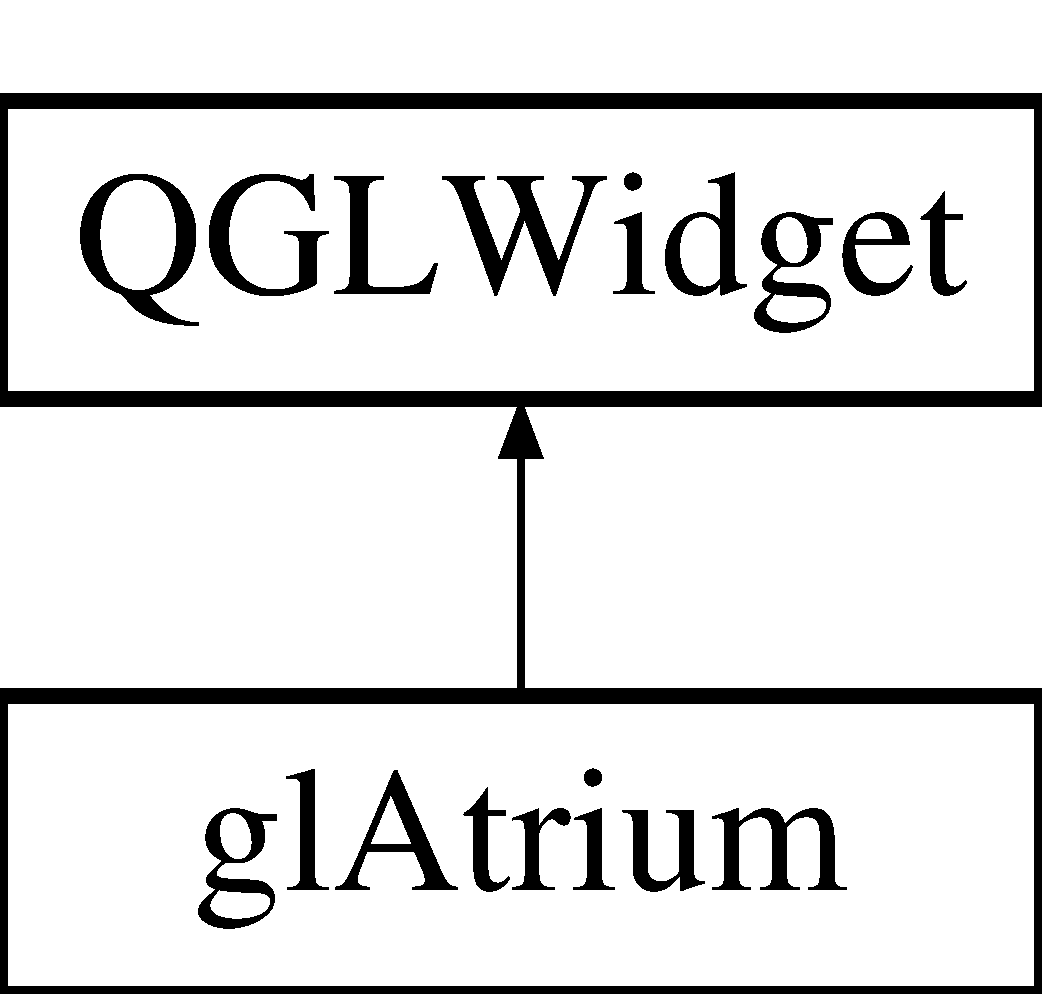
\includegraphics[height=2.000000cm]{classgl_atrium}
\end{center}
\end{figure}
\subsection*{Public Slots}
\begin{DoxyCompactItemize}
\item 
void \hyperlink{classgl_atrium_aa5afd6c2c43a3b9445e6821586671c36}{set\+X\+Rotation} (int angle)
\item 
void \hyperlink{classgl_atrium_a4b339e5080f2019dec3e916b4348f41c}{set\+Y\+Rotation} (int angle)
\item 
void \hyperlink{classgl_atrium_aab5b1212e320c13d3d3f30425f8e2028}{set\+Z\+Rotation} (int angle)
\item 
void \hyperlink{classgl_atrium_adb2aa7af154e4d83ca976bd7042726aa}{set\+Top} ()
\item 
void \hyperlink{classgl_atrium_a1ea5edb0605ee17d77d636c81dbc74a9}{set\+Side1} ()
\item 
void \hyperlink{classgl_atrium_aab139e009363e2a027e4f3a5e3f1e84b}{set\+Side2} ()
\item 
void \hyperlink{classgl_atrium_a10acfe771a3112264051aaecd87bc4d6}{set\+State\+Structure\+Modifier} (bool b)
\item 
void \hyperlink{classgl_atrium_a4712eeb59127c712ca5ed3e9ea2363d6}{set\+State\+Diffusion\+Modifier} (bool b)
\item 
void \hyperlink{classgl_atrium_a4fdc27d1e3a4b46fb4e545b5d5452656}{set\+State\+Viewer} (bool b)
\item 
void \hyperlink{classgl_atrium_a1bc8825c11be22bef34d80d8e92bba1d}{set\+State\+E\+P} (bool b)
\item 
void \hyperlink{classgl_atrium_a6c943af88177755f0dac95d12767cd22}{set\+Paint\+Conductivity} (bool b)
\item 
void \hyperlink{classgl_atrium_a4deff8ebaa4b5042643cbd1acefa7128}{set\+Paint\+E\+R\+P} (bool b)
\item 
void \hyperlink{classgl_atrium_a5a67ffc011f4545b7ecf4d8a745a6c06}{set\+Palette\+H\+S\+V} ()
\item 
void \hyperlink{classgl_atrium_acf6258aaf1d7c1a8cd7afe558bfd8fa4}{set\+Palette\+Gray} ()
\item 
void \hyperlink{classgl_atrium_a41253a382f5aa16fd076770782672661}{set\+Display\+Potential} (bool b)
\item 
void \hyperlink{classgl_atrium_a0d8ebb9fd216ef5ffa626071139ee26d}{set\+Display\+C\+S\+D} (bool b)
\item 
void \hyperlink{classgl_atrium_a7a56112f029a3a8f6943841735a12a76}{set\+Display\+Current1} (bool b)
\item 
void \hyperlink{classgl_atrium_a22f57b77572b7535269afc46a4126a53}{set\+Display\+Current2} (bool b)
\item 
void \hyperlink{classgl_atrium_a37275a26952f199c55df1ed3b38b6887}{display\+Electrogram} ()
\item 
void \hyperlink{classgl_atrium_a1b033aa6b6df0e8f73c0199ddfea108f}{set\+Outline\+Uniform} (bool b)
\item 
void \hyperlink{classgl_atrium_a2763b82810f80bd56ac251971637df46}{set\+Outline\+Gauss} (bool b)
\end{DoxyCompactItemize}
\subsection*{Signals}
\begin{DoxyCompactItemize}
\item 
void \hyperlink{classgl_atrium_add3c45ba71308914e62ac5f07d9dbce4}{x\+Rotation\+Changed} (int angle)
\item 
void \hyperlink{classgl_atrium_a12abcdbba73ff41ea8efdbbdcdbdcb6c}{y\+Rotation\+Changed} (int angle)
\item 
void \hyperlink{classgl_atrium_a71703a9bcfb404b9aa1bdab789573c7e}{z\+Rotation\+Changed} (int angle)
\end{DoxyCompactItemize}
\subsection*{Public Member Functions}
\begin{DoxyCompactItemize}
\item 
\hyperlink{classgl_atrium_a68d308b0209b6111bbbcbb56b1a5e10c}{gl\+Atrium} (\hyperlink{class_cardiac_mesh}{Cardiac\+Mesh} $\ast$link\+Mesh, \hyperlink{class_atrial_machine2d}{Atrial\+Machine2d} $\ast$link, Q\+Widget $\ast$parent=0)
\item 
\hyperlink{classgl_atrium_aab01fe62e0f7734e3b91b42a11d32db7}{$\sim$gl\+Atrium} (void)
\item 
Q\+Size \hyperlink{classgl_atrium_acf3a401dfd3ca09d8dcb36886f306ba9}{minimum\+Size\+Hint} () const 
\item 
Q\+Size \hyperlink{classgl_atrium_a0e7fc813e7c9ae4d47317109815b9705}{size\+Hint} () const 
\item 
void \hyperlink{classgl_atrium_aef6b55dd9c8a5b542c034d7bb8e6d319}{set\+Last\+Pos} (const Q\+Point \&pos)
\end{DoxyCompactItemize}
\subsection*{Public Attributes}
\begin{DoxyCompactItemize}
\item 
\hyperlink{class_cardiac_mesh}{Cardiac\+Mesh} $\ast$ \hyperlink{classgl_atrium_a8ded24946b8c91b4e1fb7f4f0545a6b0}{link\+To\+Mesh}
\item 
double \hyperlink{classgl_atrium_a2dc7a9f9a09eeb04eee7fd51e2b6d889}{paint\+Value\+Diffusion}
\begin{DoxyCompactList}\small\item\em Link to the Model. \end{DoxyCompactList}\item 
double \hyperlink{classgl_atrium_a501f9f86fd740a933a6e20efad9ff599}{paint\+Value\+E\+R\+P}
\end{DoxyCompactItemize}
\subsection*{Protected Member Functions}
\begin{DoxyCompactItemize}
\item 
void \hyperlink{classgl_atrium_a6fc7ea9064a492b562c0858eb3c44f86}{initialize\+G\+L} ()
\begin{DoxyCompactList}\small\item\em \mbox{[}1\mbox{]} \end{DoxyCompactList}\item 
void \hyperlink{classgl_atrium_a951d4caaef073f6762ddd47a409d2cf6}{paint\+G\+L} ()
\item 
void \hyperlink{classgl_atrium_a40cd7c018c743e5738560fdb4e4fea59}{resize\+G\+L} (int width, int height)
\item 
void \hyperlink{classgl_atrium_af0e47f4d5e0bc6d8cdcf16dd23c0487b}{mouse\+Press\+Event} (Q\+Mouse\+Event $\ast$event)
\item 
void \hyperlink{classgl_atrium_ad5af63d41d959d40d475d8e1aa0f6e9e}{mouse\+Move\+Event} (Q\+Mouse\+Event $\ast$event)
\item 
void \hyperlink{classgl_atrium_a3b2fff6d451823faa28b1b5f09aa384d}{mouse\+Release\+Event} (Q\+Mouse\+Event $\ast$event)
\item 
void \hyperlink{classgl_atrium_a5a4eb4614e6619d55a484cdfb733b2ea}{wheel\+Event} (Q\+Wheel\+Event $\ast$event)
\item 
Vector3 \hyperlink{classgl_atrium_a939d7c7a5289deeeea1763544e5be6b5}{screen\+To\+World} (double x, double y, double width, double height)
\item 
int \hyperlink{classgl_atrium_a02590feb7cd82c82cc67d0697136baf4}{item\+At} (double xx, double yy, double zz)
\item 
void \hyperlink{classgl_atrium_aff81827e3285b74bea0e3777a75393db}{paint\+Origin} (float scale)
\end{DoxyCompactItemize}
\subsection*{Friends}
\begin{DoxyCompactItemize}
\item 
class \hyperlink{classgl_atrium_a9879084bed338fc174a8d2fe04996ce3}{Sim\+View\+State}
\item 
class \hyperlink{classgl_atrium_a3784e26d08f8db67d4187df43944ad76}{Sim\+View\+State\+View}
\item 
class \hyperlink{classgl_atrium_a05f31e8af7a8b263cc06dbc57b20f144}{Sim\+View\+State\+Structure}
\item 
class \hyperlink{classgl_atrium_a1f495b2c4e91f752b635ad082004df63}{Sim\+View\+State\+Diffusion}
\item 
class \hyperlink{classgl_atrium_a76eb2c10fcf71ef86e90466fa0becdcb}{Sim\+View\+State\+E\+P}
\end{DoxyCompactItemize}


\subsection{Detailed Description}
T\+O\+D\+O Update to Open\+G\+L 3.\+0. 

\subsection{Constructor \& Destructor Documentation}
\hypertarget{classgl_atrium_a68d308b0209b6111bbbcbb56b1a5e10c}{\index{gl\+Atrium@{gl\+Atrium}!gl\+Atrium@{gl\+Atrium}}
\index{gl\+Atrium@{gl\+Atrium}!gl\+Atrium@{gl\+Atrium}}
\subsubsection[{gl\+Atrium}]{\setlength{\rightskip}{0pt plus 5cm}gl\+Atrium\+::gl\+Atrium (
\begin{DoxyParamCaption}
\item[{{\bf Cardiac\+Mesh} $\ast$}]{link\+Mesh, }
\item[{{\bf Atrial\+Machine2d} $\ast$}]{link, }
\item[{Q\+Widget $\ast$}]{parent = {\ttfamily 0}}
\end{DoxyParamCaption}
)}}\label{classgl_atrium_a68d308b0209b6111bbbcbb56b1a5e10c}
\hypertarget{classgl_atrium_aab01fe62e0f7734e3b91b42a11d32db7}{\index{gl\+Atrium@{gl\+Atrium}!````~gl\+Atrium@{$\sim$gl\+Atrium}}
\index{````~gl\+Atrium@{$\sim$gl\+Atrium}!gl\+Atrium@{gl\+Atrium}}
\subsubsection[{$\sim$gl\+Atrium}]{\setlength{\rightskip}{0pt plus 5cm}gl\+Atrium\+::$\sim$gl\+Atrium (
\begin{DoxyParamCaption}
\item[{void}]{}
\end{DoxyParamCaption}
)}}\label{classgl_atrium_aab01fe62e0f7734e3b91b42a11d32db7}


\subsection{Member Function Documentation}
\hypertarget{classgl_atrium_a37275a26952f199c55df1ed3b38b6887}{\index{gl\+Atrium@{gl\+Atrium}!display\+Electrogram@{display\+Electrogram}}
\index{display\+Electrogram@{display\+Electrogram}!gl\+Atrium@{gl\+Atrium}}
\subsubsection[{display\+Electrogram}]{\setlength{\rightskip}{0pt plus 5cm}void gl\+Atrium\+::display\+Electrogram (
\begin{DoxyParamCaption}
{}
\end{DoxyParamCaption}
)\hspace{0.3cm}{\ttfamily [slot]}}}\label{classgl_atrium_a37275a26952f199c55df1ed3b38b6887}
\hypertarget{classgl_atrium_a6fc7ea9064a492b562c0858eb3c44f86}{\index{gl\+Atrium@{gl\+Atrium}!initialize\+G\+L@{initialize\+G\+L}}
\index{initialize\+G\+L@{initialize\+G\+L}!gl\+Atrium@{gl\+Atrium}}
\subsubsection[{initialize\+G\+L}]{\setlength{\rightskip}{0pt plus 5cm}void gl\+Atrium\+::initialize\+G\+L (
\begin{DoxyParamCaption}
{}
\end{DoxyParamCaption}
)\hspace{0.3cm}{\ttfamily [protected]}}}\label{classgl_atrium_a6fc7ea9064a492b562c0858eb3c44f86}


\mbox{[}1\mbox{]} 

\mbox{[}2\mbox{]} \hypertarget{classgl_atrium_a02590feb7cd82c82cc67d0697136baf4}{\index{gl\+Atrium@{gl\+Atrium}!item\+At@{item\+At}}
\index{item\+At@{item\+At}!gl\+Atrium@{gl\+Atrium}}
\subsubsection[{item\+At}]{\setlength{\rightskip}{0pt plus 5cm}int gl\+Atrium\+::item\+At (
\begin{DoxyParamCaption}
\item[{double}]{xx, }
\item[{double}]{yy, }
\item[{double}]{zz}
\end{DoxyParamCaption}
)\hspace{0.3cm}{\ttfamily [protected]}}}\label{classgl_atrium_a02590feb7cd82c82cc67d0697136baf4}
\hypertarget{classgl_atrium_acf3a401dfd3ca09d8dcb36886f306ba9}{\index{gl\+Atrium@{gl\+Atrium}!minimum\+Size\+Hint@{minimum\+Size\+Hint}}
\index{minimum\+Size\+Hint@{minimum\+Size\+Hint}!gl\+Atrium@{gl\+Atrium}}
\subsubsection[{minimum\+Size\+Hint}]{\setlength{\rightskip}{0pt plus 5cm}Q\+Size gl\+Atrium\+::minimum\+Size\+Hint (
\begin{DoxyParamCaption}
{}
\end{DoxyParamCaption}
) const}}\label{classgl_atrium_acf3a401dfd3ca09d8dcb36886f306ba9}
\hypertarget{classgl_atrium_ad5af63d41d959d40d475d8e1aa0f6e9e}{\index{gl\+Atrium@{gl\+Atrium}!mouse\+Move\+Event@{mouse\+Move\+Event}}
\index{mouse\+Move\+Event@{mouse\+Move\+Event}!gl\+Atrium@{gl\+Atrium}}
\subsubsection[{mouse\+Move\+Event}]{\setlength{\rightskip}{0pt plus 5cm}void gl\+Atrium\+::mouse\+Move\+Event (
\begin{DoxyParamCaption}
\item[{Q\+Mouse\+Event $\ast$}]{event}
\end{DoxyParamCaption}
)\hspace{0.3cm}{\ttfamily [protected]}}}\label{classgl_atrium_ad5af63d41d959d40d475d8e1aa0f6e9e}
\hypertarget{classgl_atrium_af0e47f4d5e0bc6d8cdcf16dd23c0487b}{\index{gl\+Atrium@{gl\+Atrium}!mouse\+Press\+Event@{mouse\+Press\+Event}}
\index{mouse\+Press\+Event@{mouse\+Press\+Event}!gl\+Atrium@{gl\+Atrium}}
\subsubsection[{mouse\+Press\+Event}]{\setlength{\rightskip}{0pt plus 5cm}void gl\+Atrium\+::mouse\+Press\+Event (
\begin{DoxyParamCaption}
\item[{Q\+Mouse\+Event $\ast$}]{event}
\end{DoxyParamCaption}
)\hspace{0.3cm}{\ttfamily [protected]}}}\label{classgl_atrium_af0e47f4d5e0bc6d8cdcf16dd23c0487b}
\hypertarget{classgl_atrium_a3b2fff6d451823faa28b1b5f09aa384d}{\index{gl\+Atrium@{gl\+Atrium}!mouse\+Release\+Event@{mouse\+Release\+Event}}
\index{mouse\+Release\+Event@{mouse\+Release\+Event}!gl\+Atrium@{gl\+Atrium}}
\subsubsection[{mouse\+Release\+Event}]{\setlength{\rightskip}{0pt plus 5cm}void gl\+Atrium\+::mouse\+Release\+Event (
\begin{DoxyParamCaption}
\item[{Q\+Mouse\+Event $\ast$}]{event}
\end{DoxyParamCaption}
)\hspace{0.3cm}{\ttfamily [protected]}}}\label{classgl_atrium_a3b2fff6d451823faa28b1b5f09aa384d}
\hypertarget{classgl_atrium_a951d4caaef073f6762ddd47a409d2cf6}{\index{gl\+Atrium@{gl\+Atrium}!paint\+G\+L@{paint\+G\+L}}
\index{paint\+G\+L@{paint\+G\+L}!gl\+Atrium@{gl\+Atrium}}
\subsubsection[{paint\+G\+L}]{\setlength{\rightskip}{0pt plus 5cm}void gl\+Atrium\+::paint\+G\+L (
\begin{DoxyParamCaption}
{}
\end{DoxyParamCaption}
)\hspace{0.3cm}{\ttfamily [protected]}}}\label{classgl_atrium_a951d4caaef073f6762ddd47a409d2cf6}
\hypertarget{classgl_atrium_aff81827e3285b74bea0e3777a75393db}{\index{gl\+Atrium@{gl\+Atrium}!paint\+Origin@{paint\+Origin}}
\index{paint\+Origin@{paint\+Origin}!gl\+Atrium@{gl\+Atrium}}
\subsubsection[{paint\+Origin}]{\setlength{\rightskip}{0pt plus 5cm}void gl\+Atrium\+::paint\+Origin (
\begin{DoxyParamCaption}
\item[{float}]{scale}
\end{DoxyParamCaption}
)\hspace{0.3cm}{\ttfamily [protected]}}}\label{classgl_atrium_aff81827e3285b74bea0e3777a75393db}
\hypertarget{classgl_atrium_a40cd7c018c743e5738560fdb4e4fea59}{\index{gl\+Atrium@{gl\+Atrium}!resize\+G\+L@{resize\+G\+L}}
\index{resize\+G\+L@{resize\+G\+L}!gl\+Atrium@{gl\+Atrium}}
\subsubsection[{resize\+G\+L}]{\setlength{\rightskip}{0pt plus 5cm}void gl\+Atrium\+::resize\+G\+L (
\begin{DoxyParamCaption}
\item[{int}]{width, }
\item[{int}]{height}
\end{DoxyParamCaption}
)\hspace{0.3cm}{\ttfamily [protected]}}}\label{classgl_atrium_a40cd7c018c743e5738560fdb4e4fea59}
\hypertarget{classgl_atrium_a939d7c7a5289deeeea1763544e5be6b5}{\index{gl\+Atrium@{gl\+Atrium}!screen\+To\+World@{screen\+To\+World}}
\index{screen\+To\+World@{screen\+To\+World}!gl\+Atrium@{gl\+Atrium}}
\subsubsection[{screen\+To\+World}]{\setlength{\rightskip}{0pt plus 5cm}Vector3 gl\+Atrium\+::screen\+To\+World (
\begin{DoxyParamCaption}
\item[{double}]{x, }
\item[{double}]{y, }
\item[{double}]{width, }
\item[{double}]{height}
\end{DoxyParamCaption}
)\hspace{0.3cm}{\ttfamily [protected]}}}\label{classgl_atrium_a939d7c7a5289deeeea1763544e5be6b5}
\hypertarget{classgl_atrium_a0d8ebb9fd216ef5ffa626071139ee26d}{\index{gl\+Atrium@{gl\+Atrium}!set\+Display\+C\+S\+D@{set\+Display\+C\+S\+D}}
\index{set\+Display\+C\+S\+D@{set\+Display\+C\+S\+D}!gl\+Atrium@{gl\+Atrium}}
\subsubsection[{set\+Display\+C\+S\+D}]{\setlength{\rightskip}{0pt plus 5cm}void gl\+Atrium\+::set\+Display\+C\+S\+D (
\begin{DoxyParamCaption}
\item[{bool}]{b}
\end{DoxyParamCaption}
)\hspace{0.3cm}{\ttfamily [slot]}}}\label{classgl_atrium_a0d8ebb9fd216ef5ffa626071139ee26d}
\hypertarget{classgl_atrium_a7a56112f029a3a8f6943841735a12a76}{\index{gl\+Atrium@{gl\+Atrium}!set\+Display\+Current1@{set\+Display\+Current1}}
\index{set\+Display\+Current1@{set\+Display\+Current1}!gl\+Atrium@{gl\+Atrium}}
\subsubsection[{set\+Display\+Current1}]{\setlength{\rightskip}{0pt plus 5cm}void gl\+Atrium\+::set\+Display\+Current1 (
\begin{DoxyParamCaption}
\item[{bool}]{b}
\end{DoxyParamCaption}
)\hspace{0.3cm}{\ttfamily [slot]}}}\label{classgl_atrium_a7a56112f029a3a8f6943841735a12a76}
\hypertarget{classgl_atrium_a22f57b77572b7535269afc46a4126a53}{\index{gl\+Atrium@{gl\+Atrium}!set\+Display\+Current2@{set\+Display\+Current2}}
\index{set\+Display\+Current2@{set\+Display\+Current2}!gl\+Atrium@{gl\+Atrium}}
\subsubsection[{set\+Display\+Current2}]{\setlength{\rightskip}{0pt plus 5cm}void gl\+Atrium\+::set\+Display\+Current2 (
\begin{DoxyParamCaption}
\item[{bool}]{b}
\end{DoxyParamCaption}
)\hspace{0.3cm}{\ttfamily [slot]}}}\label{classgl_atrium_a22f57b77572b7535269afc46a4126a53}
\hypertarget{classgl_atrium_a41253a382f5aa16fd076770782672661}{\index{gl\+Atrium@{gl\+Atrium}!set\+Display\+Potential@{set\+Display\+Potential}}
\index{set\+Display\+Potential@{set\+Display\+Potential}!gl\+Atrium@{gl\+Atrium}}
\subsubsection[{set\+Display\+Potential}]{\setlength{\rightskip}{0pt plus 5cm}void gl\+Atrium\+::set\+Display\+Potential (
\begin{DoxyParamCaption}
\item[{bool}]{b}
\end{DoxyParamCaption}
)\hspace{0.3cm}{\ttfamily [slot]}}}\label{classgl_atrium_a41253a382f5aa16fd076770782672661}
\hypertarget{classgl_atrium_aef6b55dd9c8a5b542c034d7bb8e6d319}{\index{gl\+Atrium@{gl\+Atrium}!set\+Last\+Pos@{set\+Last\+Pos}}
\index{set\+Last\+Pos@{set\+Last\+Pos}!gl\+Atrium@{gl\+Atrium}}
\subsubsection[{set\+Last\+Pos}]{\setlength{\rightskip}{0pt plus 5cm}void gl\+Atrium\+::set\+Last\+Pos (
\begin{DoxyParamCaption}
\item[{const Q\+Point \&}]{pos}
\end{DoxyParamCaption}
)}}\label{classgl_atrium_aef6b55dd9c8a5b542c034d7bb8e6d319}
\hypertarget{classgl_atrium_a2763b82810f80bd56ac251971637df46}{\index{gl\+Atrium@{gl\+Atrium}!set\+Outline\+Gauss@{set\+Outline\+Gauss}}
\index{set\+Outline\+Gauss@{set\+Outline\+Gauss}!gl\+Atrium@{gl\+Atrium}}
\subsubsection[{set\+Outline\+Gauss}]{\setlength{\rightskip}{0pt plus 5cm}void gl\+Atrium\+::set\+Outline\+Gauss (
\begin{DoxyParamCaption}
\item[{bool}]{b}
\end{DoxyParamCaption}
)\hspace{0.3cm}{\ttfamily [slot]}}}\label{classgl_atrium_a2763b82810f80bd56ac251971637df46}
\hypertarget{classgl_atrium_a1b033aa6b6df0e8f73c0199ddfea108f}{\index{gl\+Atrium@{gl\+Atrium}!set\+Outline\+Uniform@{set\+Outline\+Uniform}}
\index{set\+Outline\+Uniform@{set\+Outline\+Uniform}!gl\+Atrium@{gl\+Atrium}}
\subsubsection[{set\+Outline\+Uniform}]{\setlength{\rightskip}{0pt plus 5cm}void gl\+Atrium\+::set\+Outline\+Uniform (
\begin{DoxyParamCaption}
\item[{bool}]{b}
\end{DoxyParamCaption}
)\hspace{0.3cm}{\ttfamily [slot]}}}\label{classgl_atrium_a1b033aa6b6df0e8f73c0199ddfea108f}
\hypertarget{classgl_atrium_a6c943af88177755f0dac95d12767cd22}{\index{gl\+Atrium@{gl\+Atrium}!set\+Paint\+Conductivity@{set\+Paint\+Conductivity}}
\index{set\+Paint\+Conductivity@{set\+Paint\+Conductivity}!gl\+Atrium@{gl\+Atrium}}
\subsubsection[{set\+Paint\+Conductivity}]{\setlength{\rightskip}{0pt plus 5cm}void gl\+Atrium\+::set\+Paint\+Conductivity (
\begin{DoxyParamCaption}
\item[{bool}]{b}
\end{DoxyParamCaption}
)\hspace{0.3cm}{\ttfamily [slot]}}}\label{classgl_atrium_a6c943af88177755f0dac95d12767cd22}
\hypertarget{classgl_atrium_a4deff8ebaa4b5042643cbd1acefa7128}{\index{gl\+Atrium@{gl\+Atrium}!set\+Paint\+E\+R\+P@{set\+Paint\+E\+R\+P}}
\index{set\+Paint\+E\+R\+P@{set\+Paint\+E\+R\+P}!gl\+Atrium@{gl\+Atrium}}
\subsubsection[{set\+Paint\+E\+R\+P}]{\setlength{\rightskip}{0pt plus 5cm}void gl\+Atrium\+::set\+Paint\+E\+R\+P (
\begin{DoxyParamCaption}
\item[{bool}]{b}
\end{DoxyParamCaption}
)\hspace{0.3cm}{\ttfamily [slot]}}}\label{classgl_atrium_a4deff8ebaa4b5042643cbd1acefa7128}
\hypertarget{classgl_atrium_acf6258aaf1d7c1a8cd7afe558bfd8fa4}{\index{gl\+Atrium@{gl\+Atrium}!set\+Palette\+Gray@{set\+Palette\+Gray}}
\index{set\+Palette\+Gray@{set\+Palette\+Gray}!gl\+Atrium@{gl\+Atrium}}
\subsubsection[{set\+Palette\+Gray}]{\setlength{\rightskip}{0pt plus 5cm}void gl\+Atrium\+::set\+Palette\+Gray (
\begin{DoxyParamCaption}
{}
\end{DoxyParamCaption}
)\hspace{0.3cm}{\ttfamily [slot]}}}\label{classgl_atrium_acf6258aaf1d7c1a8cd7afe558bfd8fa4}
\hypertarget{classgl_atrium_a5a67ffc011f4545b7ecf4d8a745a6c06}{\index{gl\+Atrium@{gl\+Atrium}!set\+Palette\+H\+S\+V@{set\+Palette\+H\+S\+V}}
\index{set\+Palette\+H\+S\+V@{set\+Palette\+H\+S\+V}!gl\+Atrium@{gl\+Atrium}}
\subsubsection[{set\+Palette\+H\+S\+V}]{\setlength{\rightskip}{0pt plus 5cm}void gl\+Atrium\+::set\+Palette\+H\+S\+V (
\begin{DoxyParamCaption}
{}
\end{DoxyParamCaption}
)\hspace{0.3cm}{\ttfamily [slot]}}}\label{classgl_atrium_a5a67ffc011f4545b7ecf4d8a745a6c06}
\hypertarget{classgl_atrium_a1ea5edb0605ee17d77d636c81dbc74a9}{\index{gl\+Atrium@{gl\+Atrium}!set\+Side1@{set\+Side1}}
\index{set\+Side1@{set\+Side1}!gl\+Atrium@{gl\+Atrium}}
\subsubsection[{set\+Side1}]{\setlength{\rightskip}{0pt plus 5cm}void gl\+Atrium\+::set\+Side1 (
\begin{DoxyParamCaption}
{}
\end{DoxyParamCaption}
)\hspace{0.3cm}{\ttfamily [slot]}}}\label{classgl_atrium_a1ea5edb0605ee17d77d636c81dbc74a9}
\hypertarget{classgl_atrium_aab139e009363e2a027e4f3a5e3f1e84b}{\index{gl\+Atrium@{gl\+Atrium}!set\+Side2@{set\+Side2}}
\index{set\+Side2@{set\+Side2}!gl\+Atrium@{gl\+Atrium}}
\subsubsection[{set\+Side2}]{\setlength{\rightskip}{0pt plus 5cm}void gl\+Atrium\+::set\+Side2 (
\begin{DoxyParamCaption}
{}
\end{DoxyParamCaption}
)\hspace{0.3cm}{\ttfamily [slot]}}}\label{classgl_atrium_aab139e009363e2a027e4f3a5e3f1e84b}
\hypertarget{classgl_atrium_a4712eeb59127c712ca5ed3e9ea2363d6}{\index{gl\+Atrium@{gl\+Atrium}!set\+State\+Diffusion\+Modifier@{set\+State\+Diffusion\+Modifier}}
\index{set\+State\+Diffusion\+Modifier@{set\+State\+Diffusion\+Modifier}!gl\+Atrium@{gl\+Atrium}}
\subsubsection[{set\+State\+Diffusion\+Modifier}]{\setlength{\rightskip}{0pt plus 5cm}void gl\+Atrium\+::set\+State\+Diffusion\+Modifier (
\begin{DoxyParamCaption}
\item[{bool}]{b}
\end{DoxyParamCaption}
)\hspace{0.3cm}{\ttfamily [slot]}}}\label{classgl_atrium_a4712eeb59127c712ca5ed3e9ea2363d6}
\hypertarget{classgl_atrium_a1bc8825c11be22bef34d80d8e92bba1d}{\index{gl\+Atrium@{gl\+Atrium}!set\+State\+E\+P@{set\+State\+E\+P}}
\index{set\+State\+E\+P@{set\+State\+E\+P}!gl\+Atrium@{gl\+Atrium}}
\subsubsection[{set\+State\+E\+P}]{\setlength{\rightskip}{0pt plus 5cm}void gl\+Atrium\+::set\+State\+E\+P (
\begin{DoxyParamCaption}
\item[{bool}]{b}
\end{DoxyParamCaption}
)\hspace{0.3cm}{\ttfamily [slot]}}}\label{classgl_atrium_a1bc8825c11be22bef34d80d8e92bba1d}
\hypertarget{classgl_atrium_a10acfe771a3112264051aaecd87bc4d6}{\index{gl\+Atrium@{gl\+Atrium}!set\+State\+Structure\+Modifier@{set\+State\+Structure\+Modifier}}
\index{set\+State\+Structure\+Modifier@{set\+State\+Structure\+Modifier}!gl\+Atrium@{gl\+Atrium}}
\subsubsection[{set\+State\+Structure\+Modifier}]{\setlength{\rightskip}{0pt plus 5cm}void gl\+Atrium\+::set\+State\+Structure\+Modifier (
\begin{DoxyParamCaption}
\item[{bool}]{b}
\end{DoxyParamCaption}
)\hspace{0.3cm}{\ttfamily [slot]}}}\label{classgl_atrium_a10acfe771a3112264051aaecd87bc4d6}
\hypertarget{classgl_atrium_a4fdc27d1e3a4b46fb4e545b5d5452656}{\index{gl\+Atrium@{gl\+Atrium}!set\+State\+Viewer@{set\+State\+Viewer}}
\index{set\+State\+Viewer@{set\+State\+Viewer}!gl\+Atrium@{gl\+Atrium}}
\subsubsection[{set\+State\+Viewer}]{\setlength{\rightskip}{0pt plus 5cm}void gl\+Atrium\+::set\+State\+Viewer (
\begin{DoxyParamCaption}
\item[{bool}]{b}
\end{DoxyParamCaption}
)\hspace{0.3cm}{\ttfamily [slot]}}}\label{classgl_atrium_a4fdc27d1e3a4b46fb4e545b5d5452656}
\hypertarget{classgl_atrium_adb2aa7af154e4d83ca976bd7042726aa}{\index{gl\+Atrium@{gl\+Atrium}!set\+Top@{set\+Top}}
\index{set\+Top@{set\+Top}!gl\+Atrium@{gl\+Atrium}}
\subsubsection[{set\+Top}]{\setlength{\rightskip}{0pt plus 5cm}void gl\+Atrium\+::set\+Top (
\begin{DoxyParamCaption}
{}
\end{DoxyParamCaption}
)\hspace{0.3cm}{\ttfamily [slot]}}}\label{classgl_atrium_adb2aa7af154e4d83ca976bd7042726aa}
\hypertarget{classgl_atrium_aa5afd6c2c43a3b9445e6821586671c36}{\index{gl\+Atrium@{gl\+Atrium}!set\+X\+Rotation@{set\+X\+Rotation}}
\index{set\+X\+Rotation@{set\+X\+Rotation}!gl\+Atrium@{gl\+Atrium}}
\subsubsection[{set\+X\+Rotation}]{\setlength{\rightskip}{0pt plus 5cm}void gl\+Atrium\+::set\+X\+Rotation (
\begin{DoxyParamCaption}
\item[{int}]{angle}
\end{DoxyParamCaption}
)\hspace{0.3cm}{\ttfamily [slot]}}}\label{classgl_atrium_aa5afd6c2c43a3b9445e6821586671c36}
\hypertarget{classgl_atrium_a4b339e5080f2019dec3e916b4348f41c}{\index{gl\+Atrium@{gl\+Atrium}!set\+Y\+Rotation@{set\+Y\+Rotation}}
\index{set\+Y\+Rotation@{set\+Y\+Rotation}!gl\+Atrium@{gl\+Atrium}}
\subsubsection[{set\+Y\+Rotation}]{\setlength{\rightskip}{0pt plus 5cm}void gl\+Atrium\+::set\+Y\+Rotation (
\begin{DoxyParamCaption}
\item[{int}]{angle}
\end{DoxyParamCaption}
)\hspace{0.3cm}{\ttfamily [slot]}}}\label{classgl_atrium_a4b339e5080f2019dec3e916b4348f41c}
\hypertarget{classgl_atrium_aab5b1212e320c13d3d3f30425f8e2028}{\index{gl\+Atrium@{gl\+Atrium}!set\+Z\+Rotation@{set\+Z\+Rotation}}
\index{set\+Z\+Rotation@{set\+Z\+Rotation}!gl\+Atrium@{gl\+Atrium}}
\subsubsection[{set\+Z\+Rotation}]{\setlength{\rightskip}{0pt plus 5cm}void gl\+Atrium\+::set\+Z\+Rotation (
\begin{DoxyParamCaption}
\item[{int}]{angle}
\end{DoxyParamCaption}
)\hspace{0.3cm}{\ttfamily [slot]}}}\label{classgl_atrium_aab5b1212e320c13d3d3f30425f8e2028}
\hypertarget{classgl_atrium_a0e7fc813e7c9ae4d47317109815b9705}{\index{gl\+Atrium@{gl\+Atrium}!size\+Hint@{size\+Hint}}
\index{size\+Hint@{size\+Hint}!gl\+Atrium@{gl\+Atrium}}
\subsubsection[{size\+Hint}]{\setlength{\rightskip}{0pt plus 5cm}Q\+Size gl\+Atrium\+::size\+Hint (
\begin{DoxyParamCaption}
{}
\end{DoxyParamCaption}
) const}}\label{classgl_atrium_a0e7fc813e7c9ae4d47317109815b9705}
\hypertarget{classgl_atrium_a5a4eb4614e6619d55a484cdfb733b2ea}{\index{gl\+Atrium@{gl\+Atrium}!wheel\+Event@{wheel\+Event}}
\index{wheel\+Event@{wheel\+Event}!gl\+Atrium@{gl\+Atrium}}
\subsubsection[{wheel\+Event}]{\setlength{\rightskip}{0pt plus 5cm}void gl\+Atrium\+::wheel\+Event (
\begin{DoxyParamCaption}
\item[{Q\+Wheel\+Event $\ast$}]{event}
\end{DoxyParamCaption}
)\hspace{0.3cm}{\ttfamily [protected]}}}\label{classgl_atrium_a5a4eb4614e6619d55a484cdfb733b2ea}
\hypertarget{classgl_atrium_add3c45ba71308914e62ac5f07d9dbce4}{\index{gl\+Atrium@{gl\+Atrium}!x\+Rotation\+Changed@{x\+Rotation\+Changed}}
\index{x\+Rotation\+Changed@{x\+Rotation\+Changed}!gl\+Atrium@{gl\+Atrium}}
\subsubsection[{x\+Rotation\+Changed}]{\setlength{\rightskip}{0pt plus 5cm}void gl\+Atrium\+::x\+Rotation\+Changed (
\begin{DoxyParamCaption}
\item[{int}]{angle}
\end{DoxyParamCaption}
)\hspace{0.3cm}{\ttfamily [signal]}}}\label{classgl_atrium_add3c45ba71308914e62ac5f07d9dbce4}
\hypertarget{classgl_atrium_a12abcdbba73ff41ea8efdbbdcdbdcb6c}{\index{gl\+Atrium@{gl\+Atrium}!y\+Rotation\+Changed@{y\+Rotation\+Changed}}
\index{y\+Rotation\+Changed@{y\+Rotation\+Changed}!gl\+Atrium@{gl\+Atrium}}
\subsubsection[{y\+Rotation\+Changed}]{\setlength{\rightskip}{0pt plus 5cm}void gl\+Atrium\+::y\+Rotation\+Changed (
\begin{DoxyParamCaption}
\item[{int}]{angle}
\end{DoxyParamCaption}
)\hspace{0.3cm}{\ttfamily [signal]}}}\label{classgl_atrium_a12abcdbba73ff41ea8efdbbdcdbdcb6c}
\hypertarget{classgl_atrium_a71703a9bcfb404b9aa1bdab789573c7e}{\index{gl\+Atrium@{gl\+Atrium}!z\+Rotation\+Changed@{z\+Rotation\+Changed}}
\index{z\+Rotation\+Changed@{z\+Rotation\+Changed}!gl\+Atrium@{gl\+Atrium}}
\subsubsection[{z\+Rotation\+Changed}]{\setlength{\rightskip}{0pt plus 5cm}void gl\+Atrium\+::z\+Rotation\+Changed (
\begin{DoxyParamCaption}
\item[{int}]{angle}
\end{DoxyParamCaption}
)\hspace{0.3cm}{\ttfamily [signal]}}}\label{classgl_atrium_a71703a9bcfb404b9aa1bdab789573c7e}


\subsection{Friends And Related Function Documentation}
\hypertarget{classgl_atrium_a9879084bed338fc174a8d2fe04996ce3}{\index{gl\+Atrium@{gl\+Atrium}!Sim\+View\+State@{Sim\+View\+State}}
\index{Sim\+View\+State@{Sim\+View\+State}!gl\+Atrium@{gl\+Atrium}}
\subsubsection[{Sim\+View\+State}]{\setlength{\rightskip}{0pt plus 5cm}friend class {\bf Sim\+View\+State}\hspace{0.3cm}{\ttfamily [friend]}}}\label{classgl_atrium_a9879084bed338fc174a8d2fe04996ce3}
\hypertarget{classgl_atrium_a1f495b2c4e91f752b635ad082004df63}{\index{gl\+Atrium@{gl\+Atrium}!Sim\+View\+State\+Diffusion@{Sim\+View\+State\+Diffusion}}
\index{Sim\+View\+State\+Diffusion@{Sim\+View\+State\+Diffusion}!gl\+Atrium@{gl\+Atrium}}
\subsubsection[{Sim\+View\+State\+Diffusion}]{\setlength{\rightskip}{0pt plus 5cm}friend class {\bf Sim\+View\+State\+Diffusion}\hspace{0.3cm}{\ttfamily [friend]}}}\label{classgl_atrium_a1f495b2c4e91f752b635ad082004df63}
\hypertarget{classgl_atrium_a76eb2c10fcf71ef86e90466fa0becdcb}{\index{gl\+Atrium@{gl\+Atrium}!Sim\+View\+State\+E\+P@{Sim\+View\+State\+E\+P}}
\index{Sim\+View\+State\+E\+P@{Sim\+View\+State\+E\+P}!gl\+Atrium@{gl\+Atrium}}
\subsubsection[{Sim\+View\+State\+E\+P}]{\setlength{\rightskip}{0pt plus 5cm}friend class {\bf Sim\+View\+State\+E\+P}\hspace{0.3cm}{\ttfamily [friend]}}}\label{classgl_atrium_a76eb2c10fcf71ef86e90466fa0becdcb}
\hypertarget{classgl_atrium_a05f31e8af7a8b263cc06dbc57b20f144}{\index{gl\+Atrium@{gl\+Atrium}!Sim\+View\+State\+Structure@{Sim\+View\+State\+Structure}}
\index{Sim\+View\+State\+Structure@{Sim\+View\+State\+Structure}!gl\+Atrium@{gl\+Atrium}}
\subsubsection[{Sim\+View\+State\+Structure}]{\setlength{\rightskip}{0pt plus 5cm}friend class {\bf Sim\+View\+State\+Structure}\hspace{0.3cm}{\ttfamily [friend]}}}\label{classgl_atrium_a05f31e8af7a8b263cc06dbc57b20f144}
\hypertarget{classgl_atrium_a3784e26d08f8db67d4187df43944ad76}{\index{gl\+Atrium@{gl\+Atrium}!Sim\+View\+State\+View@{Sim\+View\+State\+View}}
\index{Sim\+View\+State\+View@{Sim\+View\+State\+View}!gl\+Atrium@{gl\+Atrium}}
\subsubsection[{Sim\+View\+State\+View}]{\setlength{\rightskip}{0pt plus 5cm}friend class {\bf Sim\+View\+State\+View}\hspace{0.3cm}{\ttfamily [friend]}}}\label{classgl_atrium_a3784e26d08f8db67d4187df43944ad76}


\subsection{Member Data Documentation}
\hypertarget{classgl_atrium_a8ded24946b8c91b4e1fb7f4f0545a6b0}{\index{gl\+Atrium@{gl\+Atrium}!link\+To\+Mesh@{link\+To\+Mesh}}
\index{link\+To\+Mesh@{link\+To\+Mesh}!gl\+Atrium@{gl\+Atrium}}
\subsubsection[{link\+To\+Mesh}]{\setlength{\rightskip}{0pt plus 5cm}{\bf Cardiac\+Mesh}$\ast$ gl\+Atrium\+::link\+To\+Mesh}}\label{classgl_atrium_a8ded24946b8c91b4e1fb7f4f0545a6b0}
\hypertarget{classgl_atrium_a2dc7a9f9a09eeb04eee7fd51e2b6d889}{\index{gl\+Atrium@{gl\+Atrium}!paint\+Value\+Diffusion@{paint\+Value\+Diffusion}}
\index{paint\+Value\+Diffusion@{paint\+Value\+Diffusion}!gl\+Atrium@{gl\+Atrium}}
\subsubsection[{paint\+Value\+Diffusion}]{\setlength{\rightskip}{0pt plus 5cm}double gl\+Atrium\+::paint\+Value\+Diffusion}}\label{classgl_atrium_a2dc7a9f9a09eeb04eee7fd51e2b6d889}


Link to the Model. 

\hypertarget{classgl_atrium_a501f9f86fd740a933a6e20efad9ff599}{\index{gl\+Atrium@{gl\+Atrium}!paint\+Value\+E\+R\+P@{paint\+Value\+E\+R\+P}}
\index{paint\+Value\+E\+R\+P@{paint\+Value\+E\+R\+P}!gl\+Atrium@{gl\+Atrium}}
\subsubsection[{paint\+Value\+E\+R\+P}]{\setlength{\rightskip}{0pt plus 5cm}double gl\+Atrium\+::paint\+Value\+E\+R\+P}}\label{classgl_atrium_a501f9f86fd740a933a6e20efad9ff599}


The documentation for this class was generated from the following files\+:\begin{DoxyCompactItemize}
\item 
View/\hyperlink{gl_atrium_8h}{gl\+Atrium.\+h}\item 
View/\hyperlink{gl_atrium_8cpp}{gl\+Atrium.\+cpp}\end{DoxyCompactItemize}

\hypertarget{classio_handler}{\section{io\+Handler Class Reference}
\label{classio_handler}\index{io\+Handler@{io\+Handler}}
}


{\ttfamily \#include $<$io\+Handler.\+h$>$}

Inheritance diagram for io\+Handler\+:\begin{figure}[H]
\begin{center}
\leavevmode
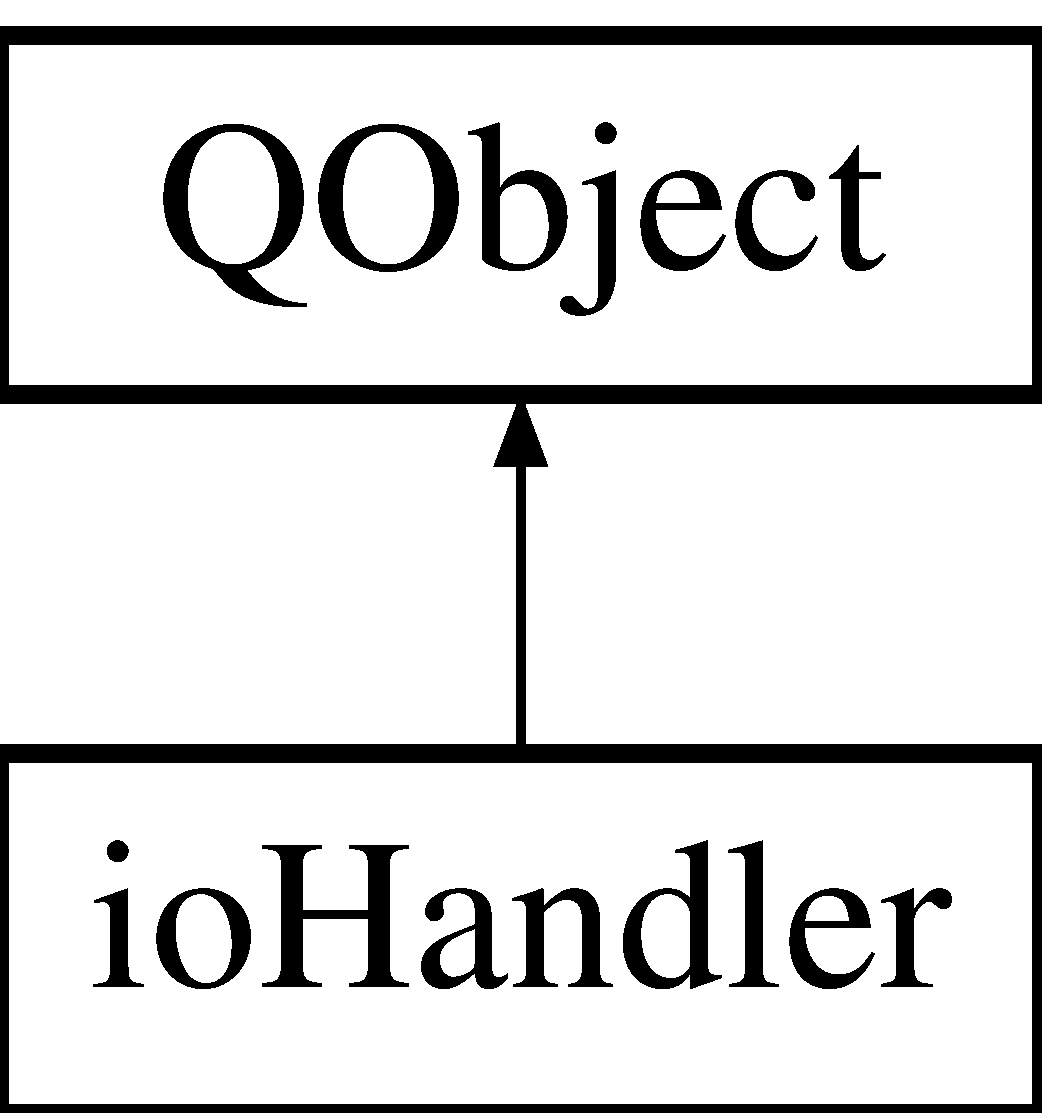
\includegraphics[height=2.000000cm]{classio_handler}
\end{center}
\end{figure}
\subsection*{Public Slots}
\begin{DoxyCompactItemize}
\item 
bool \hyperlink{classio_handler_af01b41a00277e41d62d4d80fd6fe39f7}{save\+Current\+Structure} ()
\item 
bool \hyperlink{classio_handler_a1382429c5838d6eab8195967e9c11678}{load\+Current\+State} ()
\item 
\hyperlink{class_cardiac_mesh}{Cardiac\+Mesh} $\ast$ \hyperlink{classio_handler_aabe0f6cb21a1c374fd020ff42d5c9904}{load\+Custom\+Structure} ()
\item 
bool \hyperlink{classio_handler_a59e5cd8377c13643181d9b6caef839db}{save\+Current\+State} ()
\item 
void \hyperlink{classio_handler_a472e8932c9769f3a577d11ea7c0e224d}{save\+As\+Bmp} ()
\item 
void \hyperlink{classio_handler_a8b295df2cd4f85f178935c310f6dad34}{set\+Bmp} ()
\item 
void \hyperlink{classio_handler_a0549d597c8da9195fd764044cb4c5a63}{write\+Parameters\+To\+File} ()
\item 
void \hyperlink{classio_handler_a32fc5c3861951f75c7ffbf62ed44e3e3}{get\+Parameters\+From\+File} ()
\item 
void \hyperlink{classio_handler_ac9eac90b6bdc44e46d3802e884034abe}{get\+Default\+Parameters} ()
\item 
void \hyperlink{classio_handler_a3ce2a07edc23ff12d084e64b85416954}{save\+Potential\+Plot} ()
\item 
void \hyperlink{classio_handler_aa05a5e6a55ac70333479724c48d09a42}{save\+R\+R\+Plot\+\_\+1} ()
\item 
void \hyperlink{classio_handler_aee153e33abd373472c856467563d4c7d}{save\+R\+R\+Plot\+\_\+2} ()
\item 
void \hyperlink{classio_handler_a2de36fdfa99f28b20c6fe1b2069b75ad}{save\+R\+R\+Plot\+\_\+3} ()
\end{DoxyCompactItemize}
\subsection*{Public Member Functions}
\begin{DoxyCompactItemize}
\item 
\hyperlink{classio_handler_aa57cd18c3ae379dbc508d2942ee553fa}{io\+Handler} (\hyperlink{class_simple_heart}{Simple\+Heart} $\ast$handle)
\item 
\hyperlink{classio_handler_a030878327dcdc71c410e2b3184538aed}{$\sim$io\+Handler} (void)
\item 
{\footnotesize template$<$class Ttype $>$ }\\matvar\+\_\+t $\ast$ \hyperlink{classio_handler_a217721cec0dfbacc3b564bfaa4cc7b8b}{read\+Mat\+Variable} (const char $\ast$varname, mat\+\_\+t $\ast$matfp, Ttype $\ast$\&outvar)
\item 
mat\+\_\+t $\ast$ \hyperlink{classio_handler_a98fa0fabd78d5c31b4949806ac40400d}{init\+Matlab\+Load} (const char $\ast$inname)
\item 
string \hyperlink{classio_handler_aaf8038bd0ff5a184504cf4622411fd51}{file\+Prefix} ()
\item 
string \hyperlink{classio_handler_a7d65ecb912b15cbeff8ecaa3f3a33f7b}{int\+To\+Str} (int n)
\item 
int \hyperlink{classio_handler_a24088c5418729764793ad2ff055d4de8}{str\+To\+Int} (string s)
\end{DoxyCompactItemize}
\subsection*{Public Attributes}
\begin{DoxyCompactItemize}
\item 
\hyperlink{class_simple_heart}{Simple\+Heart} $\ast$ \hyperlink{classio_handler_a69a16636ea31e6b2c16a447cc69c9d40}{m\+\_\+handle}
\item 
string \hyperlink{classio_handler_aa997341357b4da444f481ab43f455f9b}{param\+Filename}
\item 
string \hyperlink{classio_handler_a80e45be220c886422df536b4714e4b94}{m\+\_\+prefix}
\item 
Q\+String \hyperlink{classio_handler_a18b3ace510b075e81a08a4a3ed9d00a2}{path\+Parameters}
\item 
ifstream \hyperlink{classio_handler_a9eb908a81637ccd23846b8722f89a3c3}{input\+Parameters}
\item 
ofstream \hyperlink{classio_handler_a3dde6edac5ac86c95b1651faafd8b418}{backup\+Parameters}
\end{DoxyCompactItemize}


\subsection{Constructor \& Destructor Documentation}
\hypertarget{classio_handler_aa57cd18c3ae379dbc508d2942ee553fa}{\index{io\+Handler@{io\+Handler}!io\+Handler@{io\+Handler}}
\index{io\+Handler@{io\+Handler}!io\+Handler@{io\+Handler}}
\subsubsection[{io\+Handler}]{\setlength{\rightskip}{0pt plus 5cm}io\+Handler\+::io\+Handler (
\begin{DoxyParamCaption}
\item[{{\bf Simple\+Heart} $\ast$}]{handle}
\end{DoxyParamCaption}
)}}\label{classio_handler_aa57cd18c3ae379dbc508d2942ee553fa}
\hypertarget{classio_handler_a030878327dcdc71c410e2b3184538aed}{\index{io\+Handler@{io\+Handler}!````~io\+Handler@{$\sim$io\+Handler}}
\index{````~io\+Handler@{$\sim$io\+Handler}!io\+Handler@{io\+Handler}}
\subsubsection[{$\sim$io\+Handler}]{\setlength{\rightskip}{0pt plus 5cm}io\+Handler\+::$\sim$io\+Handler (
\begin{DoxyParamCaption}
\item[{void}]{}
\end{DoxyParamCaption}
)}}\label{classio_handler_a030878327dcdc71c410e2b3184538aed}


\subsection{Member Function Documentation}
\hypertarget{classio_handler_aaf8038bd0ff5a184504cf4622411fd51}{\index{io\+Handler@{io\+Handler}!file\+Prefix@{file\+Prefix}}
\index{file\+Prefix@{file\+Prefix}!io\+Handler@{io\+Handler}}
\subsubsection[{file\+Prefix}]{\setlength{\rightskip}{0pt plus 5cm}string io\+Handler\+::file\+Prefix (
\begin{DoxyParamCaption}
{}
\end{DoxyParamCaption}
)}}\label{classio_handler_aaf8038bd0ff5a184504cf4622411fd51}
\hypertarget{classio_handler_ac9eac90b6bdc44e46d3802e884034abe}{\index{io\+Handler@{io\+Handler}!get\+Default\+Parameters@{get\+Default\+Parameters}}
\index{get\+Default\+Parameters@{get\+Default\+Parameters}!io\+Handler@{io\+Handler}}
\subsubsection[{get\+Default\+Parameters}]{\setlength{\rightskip}{0pt plus 5cm}void io\+Handler\+::get\+Default\+Parameters (
\begin{DoxyParamCaption}
{}
\end{DoxyParamCaption}
)\hspace{0.3cm}{\ttfamily [slot]}}}\label{classio_handler_ac9eac90b6bdc44e46d3802e884034abe}
\hypertarget{classio_handler_a32fc5c3861951f75c7ffbf62ed44e3e3}{\index{io\+Handler@{io\+Handler}!get\+Parameters\+From\+File@{get\+Parameters\+From\+File}}
\index{get\+Parameters\+From\+File@{get\+Parameters\+From\+File}!io\+Handler@{io\+Handler}}
\subsubsection[{get\+Parameters\+From\+File}]{\setlength{\rightskip}{0pt plus 5cm}void io\+Handler\+::get\+Parameters\+From\+File (
\begin{DoxyParamCaption}
{}
\end{DoxyParamCaption}
)\hspace{0.3cm}{\ttfamily [slot]}}}\label{classio_handler_a32fc5c3861951f75c7ffbf62ed44e3e3}
\hypertarget{classio_handler_a98fa0fabd78d5c31b4949806ac40400d}{\index{io\+Handler@{io\+Handler}!init\+Matlab\+Load@{init\+Matlab\+Load}}
\index{init\+Matlab\+Load@{init\+Matlab\+Load}!io\+Handler@{io\+Handler}}
\subsubsection[{init\+Matlab\+Load}]{\setlength{\rightskip}{0pt plus 5cm}mat\+\_\+t $\ast$ io\+Handler\+::init\+Matlab\+Load (
\begin{DoxyParamCaption}
\item[{const char $\ast$}]{inname}
\end{DoxyParamCaption}
)}}\label{classio_handler_a98fa0fabd78d5c31b4949806ac40400d}
\hypertarget{classio_handler_a7d65ecb912b15cbeff8ecaa3f3a33f7b}{\index{io\+Handler@{io\+Handler}!int\+To\+Str@{int\+To\+Str}}
\index{int\+To\+Str@{int\+To\+Str}!io\+Handler@{io\+Handler}}
\subsubsection[{int\+To\+Str}]{\setlength{\rightskip}{0pt plus 5cm}string io\+Handler\+::int\+To\+Str (
\begin{DoxyParamCaption}
\item[{int}]{n}
\end{DoxyParamCaption}
)}}\label{classio_handler_a7d65ecb912b15cbeff8ecaa3f3a33f7b}
\hypertarget{classio_handler_a1382429c5838d6eab8195967e9c11678}{\index{io\+Handler@{io\+Handler}!load\+Current\+State@{load\+Current\+State}}
\index{load\+Current\+State@{load\+Current\+State}!io\+Handler@{io\+Handler}}
\subsubsection[{load\+Current\+State}]{\setlength{\rightskip}{0pt plus 5cm}bool io\+Handler\+::load\+Current\+State (
\begin{DoxyParamCaption}
{}
\end{DoxyParamCaption}
)\hspace{0.3cm}{\ttfamily [slot]}}}\label{classio_handler_a1382429c5838d6eab8195967e9c11678}
\hypertarget{classio_handler_aabe0f6cb21a1c374fd020ff42d5c9904}{\index{io\+Handler@{io\+Handler}!load\+Custom\+Structure@{load\+Custom\+Structure}}
\index{load\+Custom\+Structure@{load\+Custom\+Structure}!io\+Handler@{io\+Handler}}
\subsubsection[{load\+Custom\+Structure}]{\setlength{\rightskip}{0pt plus 5cm}{\bf Cardiac\+Mesh} $\ast$ io\+Handler\+::load\+Custom\+Structure (
\begin{DoxyParamCaption}
{}
\end{DoxyParamCaption}
)\hspace{0.3cm}{\ttfamily [slot]}}}\label{classio_handler_aabe0f6cb21a1c374fd020ff42d5c9904}
\hypertarget{classio_handler_a217721cec0dfbacc3b564bfaa4cc7b8b}{\index{io\+Handler@{io\+Handler}!read\+Mat\+Variable@{read\+Mat\+Variable}}
\index{read\+Mat\+Variable@{read\+Mat\+Variable}!io\+Handler@{io\+Handler}}
\subsubsection[{read\+Mat\+Variable}]{\setlength{\rightskip}{0pt plus 5cm}template$<$class Ttype $>$ matvar\+\_\+t $\ast$ io\+Handler\+::read\+Mat\+Variable (
\begin{DoxyParamCaption}
\item[{const char $\ast$}]{varname, }
\item[{mat\+\_\+t $\ast$}]{matfp, }
\item[{Ttype $\ast$\&}]{outvar}
\end{DoxyParamCaption}
)}}\label{classio_handler_a217721cec0dfbacc3b564bfaa4cc7b8b}
\hypertarget{classio_handler_a472e8932c9769f3a577d11ea7c0e224d}{\index{io\+Handler@{io\+Handler}!save\+As\+Bmp@{save\+As\+Bmp}}
\index{save\+As\+Bmp@{save\+As\+Bmp}!io\+Handler@{io\+Handler}}
\subsubsection[{save\+As\+Bmp}]{\setlength{\rightskip}{0pt plus 5cm}void io\+Handler\+::save\+As\+Bmp (
\begin{DoxyParamCaption}
{}
\end{DoxyParamCaption}
)\hspace{0.3cm}{\ttfamily [slot]}}}\label{classio_handler_a472e8932c9769f3a577d11ea7c0e224d}
\hypertarget{classio_handler_a59e5cd8377c13643181d9b6caef839db}{\index{io\+Handler@{io\+Handler}!save\+Current\+State@{save\+Current\+State}}
\index{save\+Current\+State@{save\+Current\+State}!io\+Handler@{io\+Handler}}
\subsubsection[{save\+Current\+State}]{\setlength{\rightskip}{0pt plus 5cm}bool io\+Handler\+::save\+Current\+State (
\begin{DoxyParamCaption}
{}
\end{DoxyParamCaption}
)\hspace{0.3cm}{\ttfamily [slot]}}}\label{classio_handler_a59e5cd8377c13643181d9b6caef839db}
\hypertarget{classio_handler_af01b41a00277e41d62d4d80fd6fe39f7}{\index{io\+Handler@{io\+Handler}!save\+Current\+Structure@{save\+Current\+Structure}}
\index{save\+Current\+Structure@{save\+Current\+Structure}!io\+Handler@{io\+Handler}}
\subsubsection[{save\+Current\+Structure}]{\setlength{\rightskip}{0pt plus 5cm}bool io\+Handler\+::save\+Current\+Structure (
\begin{DoxyParamCaption}
{}
\end{DoxyParamCaption}
)\hspace{0.3cm}{\ttfamily [slot]}}}\label{classio_handler_af01b41a00277e41d62d4d80fd6fe39f7}
\hypertarget{classio_handler_a3ce2a07edc23ff12d084e64b85416954}{\index{io\+Handler@{io\+Handler}!save\+Potential\+Plot@{save\+Potential\+Plot}}
\index{save\+Potential\+Plot@{save\+Potential\+Plot}!io\+Handler@{io\+Handler}}
\subsubsection[{save\+Potential\+Plot}]{\setlength{\rightskip}{0pt plus 5cm}void io\+Handler\+::save\+Potential\+Plot (
\begin{DoxyParamCaption}
{}
\end{DoxyParamCaption}
)\hspace{0.3cm}{\ttfamily [slot]}}}\label{classio_handler_a3ce2a07edc23ff12d084e64b85416954}
T\+O\+D\+O -\/ save log here also \hypertarget{classio_handler_aa05a5e6a55ac70333479724c48d09a42}{\index{io\+Handler@{io\+Handler}!save\+R\+R\+Plot\+\_\+1@{save\+R\+R\+Plot\+\_\+1}}
\index{save\+R\+R\+Plot\+\_\+1@{save\+R\+R\+Plot\+\_\+1}!io\+Handler@{io\+Handler}}
\subsubsection[{save\+R\+R\+Plot\+\_\+1}]{\setlength{\rightskip}{0pt plus 5cm}void io\+Handler\+::save\+R\+R\+Plot\+\_\+1 (
\begin{DoxyParamCaption}
{}
\end{DoxyParamCaption}
)\hspace{0.3cm}{\ttfamily [slot]}}}\label{classio_handler_aa05a5e6a55ac70333479724c48d09a42}
T\+O\+D\+O -\/ save log here also \hypertarget{classio_handler_aee153e33abd373472c856467563d4c7d}{\index{io\+Handler@{io\+Handler}!save\+R\+R\+Plot\+\_\+2@{save\+R\+R\+Plot\+\_\+2}}
\index{save\+R\+R\+Plot\+\_\+2@{save\+R\+R\+Plot\+\_\+2}!io\+Handler@{io\+Handler}}
\subsubsection[{save\+R\+R\+Plot\+\_\+2}]{\setlength{\rightskip}{0pt plus 5cm}void io\+Handler\+::save\+R\+R\+Plot\+\_\+2 (
\begin{DoxyParamCaption}
{}
\end{DoxyParamCaption}
)\hspace{0.3cm}{\ttfamily [slot]}}}\label{classio_handler_aee153e33abd373472c856467563d4c7d}
T\+O\+D\+O -\/ save log here also \hypertarget{classio_handler_a2de36fdfa99f28b20c6fe1b2069b75ad}{\index{io\+Handler@{io\+Handler}!save\+R\+R\+Plot\+\_\+3@{save\+R\+R\+Plot\+\_\+3}}
\index{save\+R\+R\+Plot\+\_\+3@{save\+R\+R\+Plot\+\_\+3}!io\+Handler@{io\+Handler}}
\subsubsection[{save\+R\+R\+Plot\+\_\+3}]{\setlength{\rightskip}{0pt plus 5cm}void io\+Handler\+::save\+R\+R\+Plot\+\_\+3 (
\begin{DoxyParamCaption}
{}
\end{DoxyParamCaption}
)\hspace{0.3cm}{\ttfamily [slot]}}}\label{classio_handler_a2de36fdfa99f28b20c6fe1b2069b75ad}
T\+O\+D\+O -\/ save log here also \hypertarget{classio_handler_a8b295df2cd4f85f178935c310f6dad34}{\index{io\+Handler@{io\+Handler}!set\+Bmp@{set\+Bmp}}
\index{set\+Bmp@{set\+Bmp}!io\+Handler@{io\+Handler}}
\subsubsection[{set\+Bmp}]{\setlength{\rightskip}{0pt plus 5cm}void io\+Handler\+::set\+Bmp (
\begin{DoxyParamCaption}
{}
\end{DoxyParamCaption}
)\hspace{0.3cm}{\ttfamily [slot]}}}\label{classio_handler_a8b295df2cd4f85f178935c310f6dad34}
\hypertarget{classio_handler_a24088c5418729764793ad2ff055d4de8}{\index{io\+Handler@{io\+Handler}!str\+To\+Int@{str\+To\+Int}}
\index{str\+To\+Int@{str\+To\+Int}!io\+Handler@{io\+Handler}}
\subsubsection[{str\+To\+Int}]{\setlength{\rightskip}{0pt plus 5cm}int io\+Handler\+::str\+To\+Int (
\begin{DoxyParamCaption}
\item[{string}]{s}
\end{DoxyParamCaption}
)}}\label{classio_handler_a24088c5418729764793ad2ff055d4de8}
\hypertarget{classio_handler_a0549d597c8da9195fd764044cb4c5a63}{\index{io\+Handler@{io\+Handler}!write\+Parameters\+To\+File@{write\+Parameters\+To\+File}}
\index{write\+Parameters\+To\+File@{write\+Parameters\+To\+File}!io\+Handler@{io\+Handler}}
\subsubsection[{write\+Parameters\+To\+File}]{\setlength{\rightskip}{0pt plus 5cm}void io\+Handler\+::write\+Parameters\+To\+File (
\begin{DoxyParamCaption}
{}
\end{DoxyParamCaption}
)\hspace{0.3cm}{\ttfamily [slot]}}}\label{classio_handler_a0549d597c8da9195fd764044cb4c5a63}


\subsection{Member Data Documentation}
\hypertarget{classio_handler_a3dde6edac5ac86c95b1651faafd8b418}{\index{io\+Handler@{io\+Handler}!backup\+Parameters@{backup\+Parameters}}
\index{backup\+Parameters@{backup\+Parameters}!io\+Handler@{io\+Handler}}
\subsubsection[{backup\+Parameters}]{\setlength{\rightskip}{0pt plus 5cm}ofstream io\+Handler\+::backup\+Parameters}}\label{classio_handler_a3dde6edac5ac86c95b1651faafd8b418}
\hypertarget{classio_handler_a9eb908a81637ccd23846b8722f89a3c3}{\index{io\+Handler@{io\+Handler}!input\+Parameters@{input\+Parameters}}
\index{input\+Parameters@{input\+Parameters}!io\+Handler@{io\+Handler}}
\subsubsection[{input\+Parameters}]{\setlength{\rightskip}{0pt plus 5cm}ifstream io\+Handler\+::input\+Parameters}}\label{classio_handler_a9eb908a81637ccd23846b8722f89a3c3}
\hypertarget{classio_handler_a69a16636ea31e6b2c16a447cc69c9d40}{\index{io\+Handler@{io\+Handler}!m\+\_\+handle@{m\+\_\+handle}}
\index{m\+\_\+handle@{m\+\_\+handle}!io\+Handler@{io\+Handler}}
\subsubsection[{m\+\_\+handle}]{\setlength{\rightskip}{0pt plus 5cm}{\bf Simple\+Heart}$\ast$ io\+Handler\+::m\+\_\+handle}}\label{classio_handler_a69a16636ea31e6b2c16a447cc69c9d40}
\hypertarget{classio_handler_a80e45be220c886422df536b4714e4b94}{\index{io\+Handler@{io\+Handler}!m\+\_\+prefix@{m\+\_\+prefix}}
\index{m\+\_\+prefix@{m\+\_\+prefix}!io\+Handler@{io\+Handler}}
\subsubsection[{m\+\_\+prefix}]{\setlength{\rightskip}{0pt plus 5cm}string io\+Handler\+::m\+\_\+prefix}}\label{classio_handler_a80e45be220c886422df536b4714e4b94}
\hypertarget{classio_handler_aa997341357b4da444f481ab43f455f9b}{\index{io\+Handler@{io\+Handler}!param\+Filename@{param\+Filename}}
\index{param\+Filename@{param\+Filename}!io\+Handler@{io\+Handler}}
\subsubsection[{param\+Filename}]{\setlength{\rightskip}{0pt plus 5cm}string io\+Handler\+::param\+Filename}}\label{classio_handler_aa997341357b4da444f481ab43f455f9b}
\hypertarget{classio_handler_a18b3ace510b075e81a08a4a3ed9d00a2}{\index{io\+Handler@{io\+Handler}!path\+Parameters@{path\+Parameters}}
\index{path\+Parameters@{path\+Parameters}!io\+Handler@{io\+Handler}}
\subsubsection[{path\+Parameters}]{\setlength{\rightskip}{0pt plus 5cm}Q\+String io\+Handler\+::path\+Parameters}}\label{classio_handler_a18b3ace510b075e81a08a4a3ed9d00a2}


The documentation for this class was generated from the following files\+:\begin{DoxyCompactItemize}
\item 
\hyperlink{io_handler_8h}{io\+Handler.\+h}\item 
\hyperlink{io_handler_8cpp}{io\+Handler.\+cpp}\end{DoxyCompactItemize}

\hypertarget{class_node}{\section{Node Class Reference}
\label{class_node}\index{Node@{Node}}
}


{\ttfamily \#include $<$cartesian\+Grid.\+h$>$}

\subsection*{Public Attributes}
\begin{DoxyCompactItemize}
\item 
int \hyperlink{class_node_a3e068069e57916611009bddebafa47f1}{m\+\_\+group}
\item 
double \hyperlink{class_node_a4ffb0b48da3355f3600142d3bfff9516}{m\+\_\+x}
\item 
double \hyperlink{class_node_a380511589123d85c8d759c682abcb6de}{m\+\_\+y}
\item 
Q\+Color \hyperlink{class_node_a5663077fbe17bf9ee7615ae394f2981b}{m\+\_\+color}
\item 
\hyperlink{heart_defines_8h_a2f059cd81f362503874790462d535f5b}{C\+E\+L\+L\+\_\+\+T\+Y\+P\+E} \hyperlink{class_node_a0dd069dd1d5617c728bd5d836c80a9ce}{m\+\_\+type}
\item 
bool \hyperlink{class_node_abf67558672f9f1a459612a66ebe0d3e3}{seleced1}
\item 
bool \hyperlink{class_node_a9f83516dc28d2b4f894b466290b99d5f}{seleced2}
\item 
double \hyperlink{class_node_aee39dd0e84a95339084197716d3d2d40}{m\+\_\+anisotrophy\+\_\+\+R}
\item 
double \hyperlink{class_node_a5948b728ed6427c25cf64340b18b337d}{m\+\_\+anisotrophy\+\_\+\+L}
\end{DoxyCompactItemize}


\subsection{Member Data Documentation}
\hypertarget{class_node_a5948b728ed6427c25cf64340b18b337d}{\index{Node@{Node}!m\+\_\+anisotrophy\+\_\+\+L@{m\+\_\+anisotrophy\+\_\+\+L}}
\index{m\+\_\+anisotrophy\+\_\+\+L@{m\+\_\+anisotrophy\+\_\+\+L}!Node@{Node}}
\subsubsection[{m\+\_\+anisotrophy\+\_\+\+L}]{\setlength{\rightskip}{0pt plus 5cm}double Node\+::m\+\_\+anisotrophy\+\_\+\+L}}\label{class_node_a5948b728ed6427c25cf64340b18b337d}
\hypertarget{class_node_aee39dd0e84a95339084197716d3d2d40}{\index{Node@{Node}!m\+\_\+anisotrophy\+\_\+\+R@{m\+\_\+anisotrophy\+\_\+\+R}}
\index{m\+\_\+anisotrophy\+\_\+\+R@{m\+\_\+anisotrophy\+\_\+\+R}!Node@{Node}}
\subsubsection[{m\+\_\+anisotrophy\+\_\+\+R}]{\setlength{\rightskip}{0pt plus 5cm}double Node\+::m\+\_\+anisotrophy\+\_\+\+R}}\label{class_node_aee39dd0e84a95339084197716d3d2d40}
\hypertarget{class_node_a5663077fbe17bf9ee7615ae394f2981b}{\index{Node@{Node}!m\+\_\+color@{m\+\_\+color}}
\index{m\+\_\+color@{m\+\_\+color}!Node@{Node}}
\subsubsection[{m\+\_\+color}]{\setlength{\rightskip}{0pt plus 5cm}Q\+Color Node\+::m\+\_\+color}}\label{class_node_a5663077fbe17bf9ee7615ae394f2981b}
\hypertarget{class_node_a3e068069e57916611009bddebafa47f1}{\index{Node@{Node}!m\+\_\+group@{m\+\_\+group}}
\index{m\+\_\+group@{m\+\_\+group}!Node@{Node}}
\subsubsection[{m\+\_\+group}]{\setlength{\rightskip}{0pt plus 5cm}int Node\+::m\+\_\+group}}\label{class_node_a3e068069e57916611009bddebafa47f1}
\hypertarget{class_node_a0dd069dd1d5617c728bd5d836c80a9ce}{\index{Node@{Node}!m\+\_\+type@{m\+\_\+type}}
\index{m\+\_\+type@{m\+\_\+type}!Node@{Node}}
\subsubsection[{m\+\_\+type}]{\setlength{\rightskip}{0pt plus 5cm}{\bf C\+E\+L\+L\+\_\+\+T\+Y\+P\+E} Node\+::m\+\_\+type}}\label{class_node_a0dd069dd1d5617c728bd5d836c80a9ce}
\hypertarget{class_node_a4ffb0b48da3355f3600142d3bfff9516}{\index{Node@{Node}!m\+\_\+x@{m\+\_\+x}}
\index{m\+\_\+x@{m\+\_\+x}!Node@{Node}}
\subsubsection[{m\+\_\+x}]{\setlength{\rightskip}{0pt plus 5cm}double Node\+::m\+\_\+x}}\label{class_node_a4ffb0b48da3355f3600142d3bfff9516}
\hypertarget{class_node_a380511589123d85c8d759c682abcb6de}{\index{Node@{Node}!m\+\_\+y@{m\+\_\+y}}
\index{m\+\_\+y@{m\+\_\+y}!Node@{Node}}
\subsubsection[{m\+\_\+y}]{\setlength{\rightskip}{0pt plus 5cm}double Node\+::m\+\_\+y}}\label{class_node_a380511589123d85c8d759c682abcb6de}
\hypertarget{class_node_abf67558672f9f1a459612a66ebe0d3e3}{\index{Node@{Node}!seleced1@{seleced1}}
\index{seleced1@{seleced1}!Node@{Node}}
\subsubsection[{seleced1}]{\setlength{\rightskip}{0pt plus 5cm}bool Node\+::seleced1}}\label{class_node_abf67558672f9f1a459612a66ebe0d3e3}
\hypertarget{class_node_a9f83516dc28d2b4f894b466290b99d5f}{\index{Node@{Node}!seleced2@{seleced2}}
\index{seleced2@{seleced2}!Node@{Node}}
\subsubsection[{seleced2}]{\setlength{\rightskip}{0pt plus 5cm}bool Node\+::seleced2}}\label{class_node_a9f83516dc28d2b4f894b466290b99d5f}


The documentation for this class was generated from the following file\+:\begin{DoxyCompactItemize}
\item 
Model/\hyperlink{cartesian_grid_8h}{cartesian\+Grid.\+h}\end{DoxyCompactItemize}

\hypertarget{class_numeric_strategy}{\section{Numeric\+Strategy Class Reference}
\label{class_numeric_strategy}\index{Numeric\+Strategy@{Numeric\+Strategy}}
}


{\ttfamily \#include $<$Numeric\+Strategy.\+h$>$}

Inheritance diagram for Numeric\+Strategy\+:\begin{figure}[H]
\begin{center}
\leavevmode
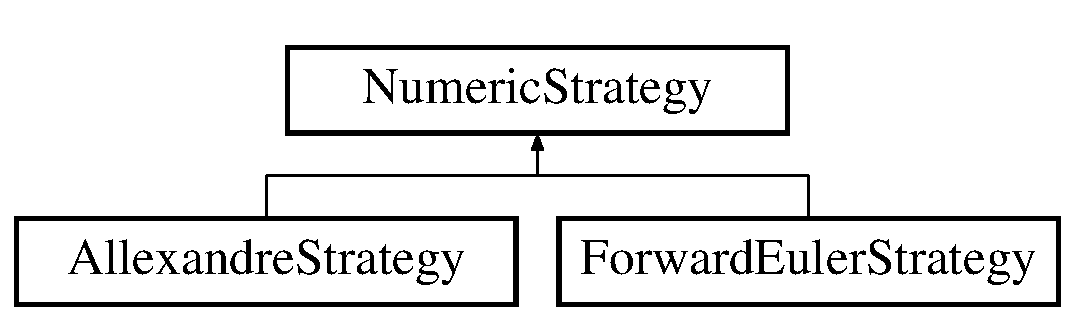
\includegraphics[height=2.000000cm]{class_numeric_strategy}
\end{center}
\end{figure}
\subsection*{Public Member Functions}
\begin{DoxyCompactItemize}
\item 
\hyperlink{class_numeric_strategy_a8f4a5e5be06427098e3a9b3635658786}{Numeric\+Strategy} (\hyperlink{class_cardiac_mesh}{Cardiac\+Mesh} $\ast$oscillators)
\item 
\hyperlink{class_numeric_strategy_ac167251a4c6409131a1be21ce3104870}{$\sim$\+Numeric\+Strategy} ()
\item 
virtual double \hyperlink{class_numeric_strategy_aeab387274e9d0ebf46a0e5ad5a5fe73f}{next\+Step} ()=0
\item 
virtual void \hyperlink{class_numeric_strategy_a81a1a510394e88edc2705e565d30f017}{reset} ()=0
\end{DoxyCompactItemize}
\subsection*{Public Attributes}
\begin{DoxyCompactItemize}
\item 
\hyperlink{class_cardiac_mesh}{Cardiac\+Mesh} $\ast$ \hyperlink{class_numeric_strategy_a2ca52f550fd3f1cc26c65aec0cacf2f6}{m\+\_\+mesh}
\end{DoxyCompactItemize}


\subsection{Constructor \& Destructor Documentation}
\hypertarget{class_numeric_strategy_a8f4a5e5be06427098e3a9b3635658786}{\index{Numeric\+Strategy@{Numeric\+Strategy}!Numeric\+Strategy@{Numeric\+Strategy}}
\index{Numeric\+Strategy@{Numeric\+Strategy}!Numeric\+Strategy@{Numeric\+Strategy}}
\subsubsection[{Numeric\+Strategy}]{\setlength{\rightskip}{0pt plus 5cm}Numeric\+Strategy\+::\+Numeric\+Strategy (
\begin{DoxyParamCaption}
\item[{{\bf Cardiac\+Mesh} $\ast$}]{oscillators}
\end{DoxyParamCaption}
)}}\label{class_numeric_strategy_a8f4a5e5be06427098e3a9b3635658786}
\hypertarget{class_numeric_strategy_ac167251a4c6409131a1be21ce3104870}{\index{Numeric\+Strategy@{Numeric\+Strategy}!````~Numeric\+Strategy@{$\sim$\+Numeric\+Strategy}}
\index{````~Numeric\+Strategy@{$\sim$\+Numeric\+Strategy}!Numeric\+Strategy@{Numeric\+Strategy}}
\subsubsection[{$\sim$\+Numeric\+Strategy}]{\setlength{\rightskip}{0pt plus 5cm}Numeric\+Strategy\+::$\sim$\+Numeric\+Strategy (
\begin{DoxyParamCaption}
{}
\end{DoxyParamCaption}
)}}\label{class_numeric_strategy_ac167251a4c6409131a1be21ce3104870}


\subsection{Member Function Documentation}
\hypertarget{class_numeric_strategy_aeab387274e9d0ebf46a0e5ad5a5fe73f}{\index{Numeric\+Strategy@{Numeric\+Strategy}!next\+Step@{next\+Step}}
\index{next\+Step@{next\+Step}!Numeric\+Strategy@{Numeric\+Strategy}}
\subsubsection[{next\+Step}]{\setlength{\rightskip}{0pt plus 5cm}virtual double Numeric\+Strategy\+::next\+Step (
\begin{DoxyParamCaption}
{}
\end{DoxyParamCaption}
)\hspace{0.3cm}{\ttfamily [pure virtual]}}}\label{class_numeric_strategy_aeab387274e9d0ebf46a0e5ad5a5fe73f}


Implemented in \hyperlink{class_allexandre_strategy_a418e280a746b6105eb609cbee6ea99fc}{Allexandre\+Strategy}, and \hyperlink{class_forward_euler_strategy_a3a382585c2d87ffaf370c07c37737a28}{Forward\+Euler\+Strategy}.

\hypertarget{class_numeric_strategy_a81a1a510394e88edc2705e565d30f017}{\index{Numeric\+Strategy@{Numeric\+Strategy}!reset@{reset}}
\index{reset@{reset}!Numeric\+Strategy@{Numeric\+Strategy}}
\subsubsection[{reset}]{\setlength{\rightskip}{0pt plus 5cm}virtual void Numeric\+Strategy\+::reset (
\begin{DoxyParamCaption}
{}
\end{DoxyParamCaption}
)\hspace{0.3cm}{\ttfamily [pure virtual]}}}\label{class_numeric_strategy_a81a1a510394e88edc2705e565d30f017}


Implemented in \hyperlink{class_allexandre_strategy_a8f657c6d14d76cef3a312fc862c400f7}{Allexandre\+Strategy}, and \hyperlink{class_forward_euler_strategy_aedd8186805189522eebfafce55617bb9}{Forward\+Euler\+Strategy}.



\subsection{Member Data Documentation}
\hypertarget{class_numeric_strategy_a2ca52f550fd3f1cc26c65aec0cacf2f6}{\index{Numeric\+Strategy@{Numeric\+Strategy}!m\+\_\+mesh@{m\+\_\+mesh}}
\index{m\+\_\+mesh@{m\+\_\+mesh}!Numeric\+Strategy@{Numeric\+Strategy}}
\subsubsection[{m\+\_\+mesh}]{\setlength{\rightskip}{0pt plus 5cm}{\bf Cardiac\+Mesh}$\ast$ Numeric\+Strategy\+::m\+\_\+mesh}}\label{class_numeric_strategy_a2ca52f550fd3f1cc26c65aec0cacf2f6}


The documentation for this class was generated from the following files\+:\begin{DoxyCompactItemize}
\item 
Numeric\+Strategy/\hyperlink{_numeric_strategy_8h}{Numeric\+Strategy.\+h}\item 
Numeric\+Strategy/\hyperlink{_numeric_strategy_8cpp}{Numeric\+Strategy.\+cpp}\end{DoxyCompactItemize}

\hypertarget{class_oscillator}{\section{Oscillator Class Reference}
\label{class_oscillator}\index{Oscillator@{Oscillator}}
}


{\ttfamily \#include $<$Oscillator.\+h$>$}

Inheritance diagram for Oscillator\+:\begin{figure}[H]
\begin{center}
\leavevmode
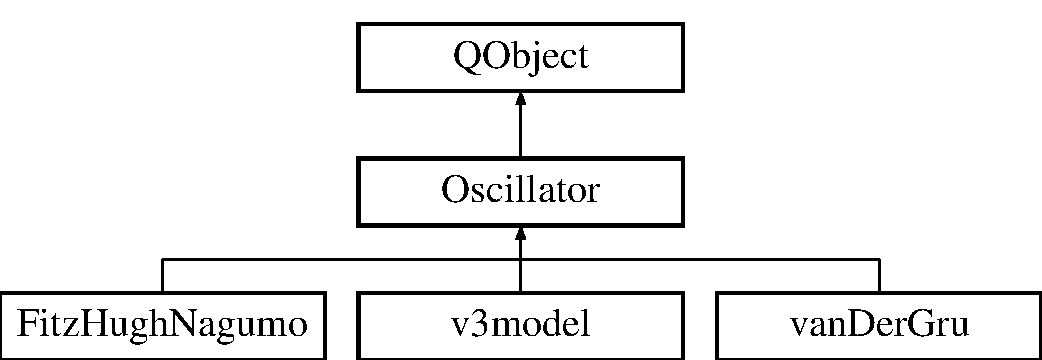
\includegraphics[height=3.000000cm]{class_oscillator}
\end{center}
\end{figure}
\subsection*{Public Slots}
\begin{DoxyCompactItemize}
\item 
virtual void \hyperlink{class_oscillator_a56140e76f42036dc6d7a4cd989917edc}{set\+Parameter} (double value, \hyperlink{heart_defines_8h_a79395aba577c2bc57e7ca211ff3476a6}{O\+S\+C\+\_\+\+P\+A\+R\+A\+M\+E\+T\+E\+R} parameter)
\end{DoxyCompactItemize}
\subsection*{Signals}
\begin{DoxyCompactItemize}
\item 
void \hyperlink{class_oscillator_a065af90ddd004f7af4e1d7489b4ea5d6}{new\+Potential\+Value} (double pot\+Value)
\item 
void \hyperlink{class_oscillator_aa48179145afe4bad7b757eefecb6053a}{new\+State} (double pot\+Value, double cur\+Value)
\item 
void \hyperlink{class_oscillator_a949a6e88a1e5b7037ba93d6a9c927b4f}{new\+Potential\+Time} (double time, double pot\+Value)
\end{DoxyCompactItemize}
\subsection*{Public Member Functions}
\begin{DoxyCompactItemize}
\item 
\hyperlink{class_oscillator_aad43fa7eeffdeb0cbc4767f2de538d80}{Oscillator} (void)
\item 
\hyperlink{class_oscillator_accb2f4ecc6604b2c38a7fd9973578360}{$\sim$\+Oscillator} (void)
\item 
void \hyperlink{class_oscillator_abc5d43aeb061d97dd58749baf2b8f82d}{state\+Calculated} (double a, double b, int which)
\item 
double \& \hyperlink{class_oscillator_a6d6d8ef3c022f6fd8c31c3e50987a822}{get\+Ref\+Potential} ()
\item 
double \& \hyperlink{class_oscillator_a734d7375586e9982a6419d1f08b63c57}{get\+Ref\+Previous\+Potential} ()
\item 
double \& \hyperlink{class_oscillator_ac82b2732257e64c0f84f5b520ef16704}{get\+Ref\+Current\+Time} ()
\item 
double \hyperlink{class_oscillator_a2dcfd98ad9d0c6e03cc07f84dd5f054a}{get\+Current} (const int \&which)
\item 
double \hyperlink{class_oscillator_a6ababfb0cb31e5dbf26b4d60a0d0bb16}{get\+Potential} ()
\item 
double \hyperlink{class_oscillator_a6272096989cb47a1cf43fd3aee78fdf5}{get\+Previous\+Potential} ()
\item 
virtual double \hyperlink{class_oscillator_a6132c7be8737a5686d64629b68b81743}{get\+Current\+Prim} (const int \&which)
\item 
virtual double \hyperlink{class_oscillator_a932fda2705d851fbe28c569547f4b4f1}{get\+Potential\+Prim} ()
\item 
double \hyperlink{class_oscillator_a6e403f6aa9e2cd9ff8aea1aefdb9459c}{get\+Current\+Time} ()
\item 
double \hyperlink{class_oscillator_a0768ee28a72db7e13e14fb717408292c}{get\+Previous\+Time} ()
\item 
\hyperlink{heart_defines_8h_a2f059cd81f362503874790462d535f5b}{C\+E\+L\+L\+\_\+\+T\+Y\+P\+E} \hyperlink{class_oscillator_aa0ae5ca40fa136d70b145d490646b8aa}{get\+Cell\+Type} ()
\item 
double \hyperlink{class_oscillator_a2eb50a29aeac6a63b4b8212d1b4cc097}{get\+Electrogram} ()
\item 
double \hyperlink{class_oscillator_a5051ab41b5036cb775faaa5f97e2c182}{get\+Extrapolated\+Neighbour\+Source} ()
\item 
double \hyperlink{class_oscillator_a38ec1c04097cceea46f4712fca7169e2}{get\+Uniform\+Timestep\+Current\+Source} ()
\item 
double \hyperlink{class_oscillator_ae0af6d579f485bc7ffbff790c145b388}{get\+Last\+Current\+Source} ()
\item 
double \hyperlink{class_oscillator_ad2be11901d2b0055a48890643db3350d}{get\+Position\+X} ()
\item 
double \hyperlink{class_oscillator_aaa999e4824d4e4007c0541ae78f60e6c}{get\+Position\+Y} ()
\item 
double \hyperlink{class_oscillator_a6f21f66ca4ca7a163d6b3d84eda3b8db}{get\+Position\+Z} ()
\item 
int \hyperlink{class_oscillator_a115350abaf2f6ddbf9c06027b8faa1e6}{get\+Number\+Of\+Currents} ()
\item 
void \hyperlink{class_oscillator_a672b578b643936b3b0b42371b6d339d9}{set\+Position\+X} (const double \&pos)
\item 
void \hyperlink{class_oscillator_aecfc7c140beecd6a82ab6d414892632d}{set\+Position\+Y} (const double \&pos)
\item 
void \hyperlink{class_oscillator_a597c5025182c90571804c6dc81f33e70}{set\+Position\+Z} (const double \&pos)
\item 
void \hyperlink{class_oscillator_acdee83b452a76ee20b48248cd4ba45cc}{set\+Type} (\hyperlink{heart_defines_8h_a2f059cd81f362503874790462d535f5b}{C\+E\+L\+L\+\_\+\+T\+Y\+P\+E} type)
\item 
void \hyperlink{class_oscillator_af5cd9a1f69c6e31748d54128a68628f8}{add\+Neighbour} (\hyperlink{class_oscillator}{Oscillator} $\ast$neighbour)
\item 
void \hyperlink{class_oscillator_a5e4ecacba9fc577660c1643c1e50e0bb}{set\+Current} (const double \&current, const int \&which)
\item 
void \hyperlink{class_oscillator_a42171f7e11ac041ab982d055ba389352}{set\+Electrogram} (const double \&electrogram)
\item 
void \hyperlink{class_oscillator_a91b56c7ed7c11f30109e8b1db296b2a6}{set\+Potential} (const double \&potential)
\item 
void \hyperlink{class_oscillator_a3e24a7637ed5aaf05101f3e115ea8e9c}{set\+Previous\+Potential} (const double \&potential)
\item 
void \hyperlink{class_oscillator_ae4fdf768b4fc00f6830c295cdc2f3e62}{set\+Current\+Time} (const double \&time)
\item 
void \hyperlink{class_oscillator_a549fcc8c0dc9a0789a062a0b1062610b}{set\+Sigma} (double s\+X, double s\+Y, double s\+Z)
\item 
void \hyperlink{class_oscillator_a8d4b8d2c8eb200afbbb4d4d999f068ab}{set\+Connexins} ()
\end{DoxyCompactItemize}
\subsection*{Public Attributes}
\begin{DoxyCompactItemize}
\item 
\hyperlink{heart_defines_8h_a2f059cd81f362503874790462d535f5b}{C\+E\+L\+L\+\_\+\+T\+Y\+P\+E} \hyperlink{class_oscillator_a7553dcea69896c2f3ff2bc8bda1d05cc}{m\+\_\+type}
\item 
int \hyperlink{class_oscillator_acfc962cfc0b6c92fc8ae8d7254346bef}{oscillator\+I\+D}
\item 
double \hyperlink{class_oscillator_a44d11f6d153d4a061fc1bbb6785ddc18}{m\+\_\+v\+\_\+potential}
\item 
double \hyperlink{class_oscillator_a2a1649ababe43b1de3dbd6d5f24db703}{m\+\_\+previous\+\_\+potential}
\item 
std\+::vector$<$ double $>$ \hyperlink{class_oscillator_a344928736ed0deb40bc1c73d50af5d33}{m\+\_\+v\+\_\+current}
\item 
double \hyperlink{class_oscillator_aedf0974c19ea8428e3702f267cf45465}{m\+\_\+potential\+P\+R\+I\+M}
\item 
std\+::vector$<$ double $>$ \hyperlink{class_oscillator_aef644a4e5faf78fa338a7a5e739f267c}{m\+\_\+current\+P\+R\+I\+M}
\item 
double \hyperlink{class_oscillator_ab65a59d93c248616facbd1f01b3c2b87}{m\+\_\+v\+\_\+electrogram}
\item 
double \hyperlink{class_oscillator_aae4aa22ad331c19871be91d7cc5ceafa}{m\+\_\+v\+\_\+scaled\+Potential}
\item 
double \hyperlink{class_oscillator_a45a1214b84b342e4ee078d218112f001}{m\+\_\+previous\+\_\+scaled\+Potential}
\item 
double \hyperlink{class_oscillator_abe68e99fc990a44b9bd234751eec0f24}{m\+\_\+current\+Time}
\item 
double \hyperlink{class_oscillator_ab97f31715485a24f49c98a01caa9f2d8}{m\+\_\+previous\+Time}
\item 
double \hyperlink{class_oscillator_a4db30c0516d078b69426aad65bf13022}{guard\+Timestep}
\item 
bool \hyperlink{class_oscillator_aeaa03f804f9d13f27635b94ea7a6bd32}{m\+\_\+under\+Stimulation}
\item 
double \hyperlink{class_oscillator_a968627d069d5f0c44d8134718a01237f}{\+\_\+source\+A}
\item 
double \hyperlink{class_oscillator_a5a144fd5dd7cbcbfc47d7c9013d330b8}{\+\_\+source\+B}
\item 
double \hyperlink{class_oscillator_a766694982f9a1f8ed7013828089587f7}{m\+\_\+current\+Source}
\item 
double \hyperlink{class_oscillator_abd8b2a7267f85cae787a0bc77d1f5a5a}{m\+\_\+x}
\item 
double \hyperlink{class_oscillator_a6936c789a75680f0486c817af4fce202}{m\+\_\+y}
\item 
double \hyperlink{class_oscillator_ae00491a4783797fb6edb9c3d5317a6ad}{m\+\_\+z}
\item 
double \hyperlink{class_oscillator_aa0fe6259ca35433e3bd0dbac2d0ead65}{m\+\_\+sigma\+X}
\item 
double \hyperlink{class_oscillator_a253c7652df4789833c9f940c3278036d}{m\+\_\+sigma\+Y}
\item 
double \hyperlink{class_oscillator_af8ba90eb71c73ac1c789d569e7e2f92f}{m\+\_\+sigma\+Z}
\item 
double \hyperlink{class_oscillator_a952e781ffe848b06b7b511c54f1d090c}{m\+\_\+\+Connexin\+Sum}
\item 
std\+::vector$<$ \hyperlink{class_oscillator}{Oscillator} $\ast$ $>$ \hyperlink{class_oscillator_ac6add7bad19c62071ad1ce651b815e4e}{m\+\_\+neighbours}
\item 
std\+::vector$<$ double $>$ \hyperlink{class_oscillator_a7031173912bc2225997a3ab6f9995fec}{m\+\_\+neighbours\+Distance}
\item 
std\+::vector$<$ double $>$ \hyperlink{class_oscillator_a94d86971a2a425d2e2492962491dc01b}{m\+\_\+connexin}
\item 
double \hyperlink{class_oscillator_a80a2b0beda0d17f549160fbbd456243b}{m\+\_\+hormonal\+Activity}
\item 
double \hyperlink{class_oscillator_a43006eaf9a5a3b50a8f6a2a95ce47231}{vmax}
\item 
double \hyperlink{class_oscillator_a8912b5faff383dcc1a33554d2bcc5844}{vmin}
\item 
double \hyperlink{class_oscillator_af6886099dfca8ec732676f4f89935651}{vzero}
\end{DoxyCompactItemize}


\subsection{Constructor \& Destructor Documentation}
\hypertarget{class_oscillator_aad43fa7eeffdeb0cbc4767f2de538d80}{\index{Oscillator@{Oscillator}!Oscillator@{Oscillator}}
\index{Oscillator@{Oscillator}!Oscillator@{Oscillator}}
\subsubsection[{Oscillator}]{\setlength{\rightskip}{0pt plus 5cm}Oscillator\+::\+Oscillator (
\begin{DoxyParamCaption}
\item[{void}]{}
\end{DoxyParamCaption}
)}}\label{class_oscillator_aad43fa7eeffdeb0cbc4767f2de538d80}
\hypertarget{class_oscillator_accb2f4ecc6604b2c38a7fd9973578360}{\index{Oscillator@{Oscillator}!````~Oscillator@{$\sim$\+Oscillator}}
\index{````~Oscillator@{$\sim$\+Oscillator}!Oscillator@{Oscillator}}
\subsubsection[{$\sim$\+Oscillator}]{\setlength{\rightskip}{0pt plus 5cm}Oscillator\+::$\sim$\+Oscillator (
\begin{DoxyParamCaption}
\item[{void}]{}
\end{DoxyParamCaption}
)}}\label{class_oscillator_accb2f4ecc6604b2c38a7fd9973578360}


\subsection{Member Function Documentation}
\hypertarget{class_oscillator_af5cd9a1f69c6e31748d54128a68628f8}{\index{Oscillator@{Oscillator}!add\+Neighbour@{add\+Neighbour}}
\index{add\+Neighbour@{add\+Neighbour}!Oscillator@{Oscillator}}
\subsubsection[{add\+Neighbour}]{\setlength{\rightskip}{0pt plus 5cm}void Oscillator\+::add\+Neighbour (
\begin{DoxyParamCaption}
\item[{{\bf Oscillator} $\ast$}]{neighbour}
\end{DoxyParamCaption}
)}}\label{class_oscillator_af5cd9a1f69c6e31748d54128a68628f8}
\hypertarget{class_oscillator_aa0ae5ca40fa136d70b145d490646b8aa}{\index{Oscillator@{Oscillator}!get\+Cell\+Type@{get\+Cell\+Type}}
\index{get\+Cell\+Type@{get\+Cell\+Type}!Oscillator@{Oscillator}}
\subsubsection[{get\+Cell\+Type}]{\setlength{\rightskip}{0pt plus 5cm}{\bf C\+E\+L\+L\+\_\+\+T\+Y\+P\+E} Oscillator\+::get\+Cell\+Type (
\begin{DoxyParamCaption}
{}
\end{DoxyParamCaption}
)}}\label{class_oscillator_aa0ae5ca40fa136d70b145d490646b8aa}
\hypertarget{class_oscillator_a2dcfd98ad9d0c6e03cc07f84dd5f054a}{\index{Oscillator@{Oscillator}!get\+Current@{get\+Current}}
\index{get\+Current@{get\+Current}!Oscillator@{Oscillator}}
\subsubsection[{get\+Current}]{\setlength{\rightskip}{0pt plus 5cm}double Oscillator\+::get\+Current (
\begin{DoxyParamCaption}
\item[{const int \&}]{which}
\end{DoxyParamCaption}
)}}\label{class_oscillator_a2dcfd98ad9d0c6e03cc07f84dd5f054a}
\hypertarget{class_oscillator_a6132c7be8737a5686d64629b68b81743}{\index{Oscillator@{Oscillator}!get\+Current\+Prim@{get\+Current\+Prim}}
\index{get\+Current\+Prim@{get\+Current\+Prim}!Oscillator@{Oscillator}}
\subsubsection[{get\+Current\+Prim}]{\setlength{\rightskip}{0pt plus 5cm}double Oscillator\+::get\+Current\+Prim (
\begin{DoxyParamCaption}
\item[{const int \&}]{which}
\end{DoxyParamCaption}
)\hspace{0.3cm}{\ttfamily [virtual]}}}\label{class_oscillator_a6132c7be8737a5686d64629b68b81743}


Reimplemented in \hyperlink{classv3model_a14957985c821508b7a5985a423d0c942}{v3model}.

\hypertarget{class_oscillator_a6e403f6aa9e2cd9ff8aea1aefdb9459c}{\index{Oscillator@{Oscillator}!get\+Current\+Time@{get\+Current\+Time}}
\index{get\+Current\+Time@{get\+Current\+Time}!Oscillator@{Oscillator}}
\subsubsection[{get\+Current\+Time}]{\setlength{\rightskip}{0pt plus 5cm}double Oscillator\+::get\+Current\+Time (
\begin{DoxyParamCaption}
{}
\end{DoxyParamCaption}
)}}\label{class_oscillator_a6e403f6aa9e2cd9ff8aea1aefdb9459c}
\hypertarget{class_oscillator_a2eb50a29aeac6a63b4b8212d1b4cc097}{\index{Oscillator@{Oscillator}!get\+Electrogram@{get\+Electrogram}}
\index{get\+Electrogram@{get\+Electrogram}!Oscillator@{Oscillator}}
\subsubsection[{get\+Electrogram}]{\setlength{\rightskip}{0pt plus 5cm}double Oscillator\+::get\+Electrogram (
\begin{DoxyParamCaption}
{}
\end{DoxyParamCaption}
)}}\label{class_oscillator_a2eb50a29aeac6a63b4b8212d1b4cc097}
\hypertarget{class_oscillator_a5051ab41b5036cb775faaa5f97e2c182}{\index{Oscillator@{Oscillator}!get\+Extrapolated\+Neighbour\+Source@{get\+Extrapolated\+Neighbour\+Source}}
\index{get\+Extrapolated\+Neighbour\+Source@{get\+Extrapolated\+Neighbour\+Source}!Oscillator@{Oscillator}}
\subsubsection[{get\+Extrapolated\+Neighbour\+Source}]{\setlength{\rightskip}{0pt plus 5cm}double Oscillator\+::get\+Extrapolated\+Neighbour\+Source (
\begin{DoxyParamCaption}
{}
\end{DoxyParamCaption}
)}}\label{class_oscillator_a5051ab41b5036cb775faaa5f97e2c182}
\hypertarget{class_oscillator_ae0af6d579f485bc7ffbff790c145b388}{\index{Oscillator@{Oscillator}!get\+Last\+Current\+Source@{get\+Last\+Current\+Source}}
\index{get\+Last\+Current\+Source@{get\+Last\+Current\+Source}!Oscillator@{Oscillator}}
\subsubsection[{get\+Last\+Current\+Source}]{\setlength{\rightskip}{0pt plus 5cm}double Oscillator\+::get\+Last\+Current\+Source (
\begin{DoxyParamCaption}
{}
\end{DoxyParamCaption}
)}}\label{class_oscillator_ae0af6d579f485bc7ffbff790c145b388}
\hypertarget{class_oscillator_a115350abaf2f6ddbf9c06027b8faa1e6}{\index{Oscillator@{Oscillator}!get\+Number\+Of\+Currents@{get\+Number\+Of\+Currents}}
\index{get\+Number\+Of\+Currents@{get\+Number\+Of\+Currents}!Oscillator@{Oscillator}}
\subsubsection[{get\+Number\+Of\+Currents}]{\setlength{\rightskip}{0pt plus 5cm}int Oscillator\+::get\+Number\+Of\+Currents (
\begin{DoxyParamCaption}
{}
\end{DoxyParamCaption}
)}}\label{class_oscillator_a115350abaf2f6ddbf9c06027b8faa1e6}
\hypertarget{class_oscillator_ad2be11901d2b0055a48890643db3350d}{\index{Oscillator@{Oscillator}!get\+Position\+X@{get\+Position\+X}}
\index{get\+Position\+X@{get\+Position\+X}!Oscillator@{Oscillator}}
\subsubsection[{get\+Position\+X}]{\setlength{\rightskip}{0pt plus 5cm}double Oscillator\+::get\+Position\+X (
\begin{DoxyParamCaption}
{}
\end{DoxyParamCaption}
)}}\label{class_oscillator_ad2be11901d2b0055a48890643db3350d}
\hypertarget{class_oscillator_aaa999e4824d4e4007c0541ae78f60e6c}{\index{Oscillator@{Oscillator}!get\+Position\+Y@{get\+Position\+Y}}
\index{get\+Position\+Y@{get\+Position\+Y}!Oscillator@{Oscillator}}
\subsubsection[{get\+Position\+Y}]{\setlength{\rightskip}{0pt plus 5cm}double Oscillator\+::get\+Position\+Y (
\begin{DoxyParamCaption}
{}
\end{DoxyParamCaption}
)}}\label{class_oscillator_aaa999e4824d4e4007c0541ae78f60e6c}
\hypertarget{class_oscillator_a6f21f66ca4ca7a163d6b3d84eda3b8db}{\index{Oscillator@{Oscillator}!get\+Position\+Z@{get\+Position\+Z}}
\index{get\+Position\+Z@{get\+Position\+Z}!Oscillator@{Oscillator}}
\subsubsection[{get\+Position\+Z}]{\setlength{\rightskip}{0pt plus 5cm}double Oscillator\+::get\+Position\+Z (
\begin{DoxyParamCaption}
{}
\end{DoxyParamCaption}
)}}\label{class_oscillator_a6f21f66ca4ca7a163d6b3d84eda3b8db}
\hypertarget{class_oscillator_a6ababfb0cb31e5dbf26b4d60a0d0bb16}{\index{Oscillator@{Oscillator}!get\+Potential@{get\+Potential}}
\index{get\+Potential@{get\+Potential}!Oscillator@{Oscillator}}
\subsubsection[{get\+Potential}]{\setlength{\rightskip}{0pt plus 5cm}double Oscillator\+::get\+Potential (
\begin{DoxyParamCaption}
{}
\end{DoxyParamCaption}
)}}\label{class_oscillator_a6ababfb0cb31e5dbf26b4d60a0d0bb16}
\hypertarget{class_oscillator_a932fda2705d851fbe28c569547f4b4f1}{\index{Oscillator@{Oscillator}!get\+Potential\+Prim@{get\+Potential\+Prim}}
\index{get\+Potential\+Prim@{get\+Potential\+Prim}!Oscillator@{Oscillator}}
\subsubsection[{get\+Potential\+Prim}]{\setlength{\rightskip}{0pt plus 5cm}double Oscillator\+::get\+Potential\+Prim (
\begin{DoxyParamCaption}
{}
\end{DoxyParamCaption}
)\hspace{0.3cm}{\ttfamily [virtual]}}}\label{class_oscillator_a932fda2705d851fbe28c569547f4b4f1}


Reimplemented in \hyperlink{classv3model_a7db295a02c2487b6eb4d13e6e942a088}{v3model}, \hyperlink{class_fitz_hugh_nagumo_ae4d4e8c1c3b9905a0e6aaa5ae0c2f2ed}{Fitz\+Hugh\+Nagumo}, and \hyperlink{classvan_der_gru_afe764c0c671b5a1f7cbf21f87f5eb936}{van\+Der\+Gru}.

\hypertarget{class_oscillator_a6272096989cb47a1cf43fd3aee78fdf5}{\index{Oscillator@{Oscillator}!get\+Previous\+Potential@{get\+Previous\+Potential}}
\index{get\+Previous\+Potential@{get\+Previous\+Potential}!Oscillator@{Oscillator}}
\subsubsection[{get\+Previous\+Potential}]{\setlength{\rightskip}{0pt plus 5cm}double Oscillator\+::get\+Previous\+Potential (
\begin{DoxyParamCaption}
{}
\end{DoxyParamCaption}
)}}\label{class_oscillator_a6272096989cb47a1cf43fd3aee78fdf5}
\hypertarget{class_oscillator_a0768ee28a72db7e13e14fb717408292c}{\index{Oscillator@{Oscillator}!get\+Previous\+Time@{get\+Previous\+Time}}
\index{get\+Previous\+Time@{get\+Previous\+Time}!Oscillator@{Oscillator}}
\subsubsection[{get\+Previous\+Time}]{\setlength{\rightskip}{0pt plus 5cm}double Oscillator\+::get\+Previous\+Time (
\begin{DoxyParamCaption}
{}
\end{DoxyParamCaption}
)}}\label{class_oscillator_a0768ee28a72db7e13e14fb717408292c}
\hypertarget{class_oscillator_ac82b2732257e64c0f84f5b520ef16704}{\index{Oscillator@{Oscillator}!get\+Ref\+Current\+Time@{get\+Ref\+Current\+Time}}
\index{get\+Ref\+Current\+Time@{get\+Ref\+Current\+Time}!Oscillator@{Oscillator}}
\subsubsection[{get\+Ref\+Current\+Time}]{\setlength{\rightskip}{0pt plus 5cm}double \& Oscillator\+::get\+Ref\+Current\+Time (
\begin{DoxyParamCaption}
{}
\end{DoxyParamCaption}
)}}\label{class_oscillator_ac82b2732257e64c0f84f5b520ef16704}
\hypertarget{class_oscillator_a6d6d8ef3c022f6fd8c31c3e50987a822}{\index{Oscillator@{Oscillator}!get\+Ref\+Potential@{get\+Ref\+Potential}}
\index{get\+Ref\+Potential@{get\+Ref\+Potential}!Oscillator@{Oscillator}}
\subsubsection[{get\+Ref\+Potential}]{\setlength{\rightskip}{0pt plus 5cm}double \& Oscillator\+::get\+Ref\+Potential (
\begin{DoxyParamCaption}
{}
\end{DoxyParamCaption}
)}}\label{class_oscillator_a6d6d8ef3c022f6fd8c31c3e50987a822}
\hypertarget{class_oscillator_a734d7375586e9982a6419d1f08b63c57}{\index{Oscillator@{Oscillator}!get\+Ref\+Previous\+Potential@{get\+Ref\+Previous\+Potential}}
\index{get\+Ref\+Previous\+Potential@{get\+Ref\+Previous\+Potential}!Oscillator@{Oscillator}}
\subsubsection[{get\+Ref\+Previous\+Potential}]{\setlength{\rightskip}{0pt plus 5cm}double \& Oscillator\+::get\+Ref\+Previous\+Potential (
\begin{DoxyParamCaption}
{}
\end{DoxyParamCaption}
)}}\label{class_oscillator_a734d7375586e9982a6419d1f08b63c57}
\hypertarget{class_oscillator_a38ec1c04097cceea46f4712fca7169e2}{\index{Oscillator@{Oscillator}!get\+Uniform\+Timestep\+Current\+Source@{get\+Uniform\+Timestep\+Current\+Source}}
\index{get\+Uniform\+Timestep\+Current\+Source@{get\+Uniform\+Timestep\+Current\+Source}!Oscillator@{Oscillator}}
\subsubsection[{get\+Uniform\+Timestep\+Current\+Source}]{\setlength{\rightskip}{0pt plus 5cm}double Oscillator\+::get\+Uniform\+Timestep\+Current\+Source (
\begin{DoxyParamCaption}
{}
\end{DoxyParamCaption}
)}}\label{class_oscillator_a38ec1c04097cceea46f4712fca7169e2}
\hypertarget{class_oscillator_a949a6e88a1e5b7037ba93d6a9c927b4f}{\index{Oscillator@{Oscillator}!new\+Potential\+Time@{new\+Potential\+Time}}
\index{new\+Potential\+Time@{new\+Potential\+Time}!Oscillator@{Oscillator}}
\subsubsection[{new\+Potential\+Time}]{\setlength{\rightskip}{0pt plus 5cm}void Oscillator\+::new\+Potential\+Time (
\begin{DoxyParamCaption}
\item[{double}]{time, }
\item[{double}]{pot\+Value}
\end{DoxyParamCaption}
)\hspace{0.3cm}{\ttfamily [signal]}}}\label{class_oscillator_a949a6e88a1e5b7037ba93d6a9c927b4f}
\hypertarget{class_oscillator_a065af90ddd004f7af4e1d7489b4ea5d6}{\index{Oscillator@{Oscillator}!new\+Potential\+Value@{new\+Potential\+Value}}
\index{new\+Potential\+Value@{new\+Potential\+Value}!Oscillator@{Oscillator}}
\subsubsection[{new\+Potential\+Value}]{\setlength{\rightskip}{0pt plus 5cm}void Oscillator\+::new\+Potential\+Value (
\begin{DoxyParamCaption}
\item[{double}]{pot\+Value}
\end{DoxyParamCaption}
)\hspace{0.3cm}{\ttfamily [signal]}}}\label{class_oscillator_a065af90ddd004f7af4e1d7489b4ea5d6}
\hypertarget{class_oscillator_aa48179145afe4bad7b757eefecb6053a}{\index{Oscillator@{Oscillator}!new\+State@{new\+State}}
\index{new\+State@{new\+State}!Oscillator@{Oscillator}}
\subsubsection[{new\+State}]{\setlength{\rightskip}{0pt plus 5cm}void Oscillator\+::new\+State (
\begin{DoxyParamCaption}
\item[{double}]{pot\+Value, }
\item[{double}]{cur\+Value}
\end{DoxyParamCaption}
)\hspace{0.3cm}{\ttfamily [signal]}}}\label{class_oscillator_aa48179145afe4bad7b757eefecb6053a}
\hypertarget{class_oscillator_a8d4b8d2c8eb200afbbb4d4d999f068ab}{\index{Oscillator@{Oscillator}!set\+Connexins@{set\+Connexins}}
\index{set\+Connexins@{set\+Connexins}!Oscillator@{Oscillator}}
\subsubsection[{set\+Connexins}]{\setlength{\rightskip}{0pt plus 5cm}void Oscillator\+::set\+Connexins (
\begin{DoxyParamCaption}
{}
\end{DoxyParamCaption}
)}}\label{class_oscillator_a8d4b8d2c8eb200afbbb4d4d999f068ab}
\hypertarget{class_oscillator_a5e4ecacba9fc577660c1643c1e50e0bb}{\index{Oscillator@{Oscillator}!set\+Current@{set\+Current}}
\index{set\+Current@{set\+Current}!Oscillator@{Oscillator}}
\subsubsection[{set\+Current}]{\setlength{\rightskip}{0pt plus 5cm}void Oscillator\+::set\+Current (
\begin{DoxyParamCaption}
\item[{const double \&}]{current, }
\item[{const int \&}]{which}
\end{DoxyParamCaption}
)}}\label{class_oscillator_a5e4ecacba9fc577660c1643c1e50e0bb}
\hypertarget{class_oscillator_ae4fdf768b4fc00f6830c295cdc2f3e62}{\index{Oscillator@{Oscillator}!set\+Current\+Time@{set\+Current\+Time}}
\index{set\+Current\+Time@{set\+Current\+Time}!Oscillator@{Oscillator}}
\subsubsection[{set\+Current\+Time}]{\setlength{\rightskip}{0pt plus 5cm}void Oscillator\+::set\+Current\+Time (
\begin{DoxyParamCaption}
\item[{const double \&}]{time}
\end{DoxyParamCaption}
)}}\label{class_oscillator_ae4fdf768b4fc00f6830c295cdc2f3e62}
\hypertarget{class_oscillator_a42171f7e11ac041ab982d055ba389352}{\index{Oscillator@{Oscillator}!set\+Electrogram@{set\+Electrogram}}
\index{set\+Electrogram@{set\+Electrogram}!Oscillator@{Oscillator}}
\subsubsection[{set\+Electrogram}]{\setlength{\rightskip}{0pt plus 5cm}void Oscillator\+::set\+Electrogram (
\begin{DoxyParamCaption}
\item[{const double \&}]{electrogram}
\end{DoxyParamCaption}
)}}\label{class_oscillator_a42171f7e11ac041ab982d055ba389352}
\hypertarget{class_oscillator_a56140e76f42036dc6d7a4cd989917edc}{\index{Oscillator@{Oscillator}!set\+Parameter@{set\+Parameter}}
\index{set\+Parameter@{set\+Parameter}!Oscillator@{Oscillator}}
\subsubsection[{set\+Parameter}]{\setlength{\rightskip}{0pt plus 5cm}void Oscillator\+::set\+Parameter (
\begin{DoxyParamCaption}
\item[{double}]{value, }
\item[{{\bf O\+S\+C\+\_\+\+P\+A\+R\+A\+M\+E\+T\+E\+R}}]{parameter}
\end{DoxyParamCaption}
)\hspace{0.3cm}{\ttfamily [virtual]}, {\ttfamily [slot]}}}\label{class_oscillator_a56140e76f42036dc6d7a4cd989917edc}
\hypertarget{class_oscillator_a672b578b643936b3b0b42371b6d339d9}{\index{Oscillator@{Oscillator}!set\+Position\+X@{set\+Position\+X}}
\index{set\+Position\+X@{set\+Position\+X}!Oscillator@{Oscillator}}
\subsubsection[{set\+Position\+X}]{\setlength{\rightskip}{0pt plus 5cm}void Oscillator\+::set\+Position\+X (
\begin{DoxyParamCaption}
\item[{const double \&}]{pos}
\end{DoxyParamCaption}
)}}\label{class_oscillator_a672b578b643936b3b0b42371b6d339d9}
\hypertarget{class_oscillator_aecfc7c140beecd6a82ab6d414892632d}{\index{Oscillator@{Oscillator}!set\+Position\+Y@{set\+Position\+Y}}
\index{set\+Position\+Y@{set\+Position\+Y}!Oscillator@{Oscillator}}
\subsubsection[{set\+Position\+Y}]{\setlength{\rightskip}{0pt plus 5cm}void Oscillator\+::set\+Position\+Y (
\begin{DoxyParamCaption}
\item[{const double \&}]{pos}
\end{DoxyParamCaption}
)}}\label{class_oscillator_aecfc7c140beecd6a82ab6d414892632d}
\hypertarget{class_oscillator_a597c5025182c90571804c6dc81f33e70}{\index{Oscillator@{Oscillator}!set\+Position\+Z@{set\+Position\+Z}}
\index{set\+Position\+Z@{set\+Position\+Z}!Oscillator@{Oscillator}}
\subsubsection[{set\+Position\+Z}]{\setlength{\rightskip}{0pt plus 5cm}void Oscillator\+::set\+Position\+Z (
\begin{DoxyParamCaption}
\item[{const double \&}]{pos}
\end{DoxyParamCaption}
)}}\label{class_oscillator_a597c5025182c90571804c6dc81f33e70}
\hypertarget{class_oscillator_a91b56c7ed7c11f30109e8b1db296b2a6}{\index{Oscillator@{Oscillator}!set\+Potential@{set\+Potential}}
\index{set\+Potential@{set\+Potential}!Oscillator@{Oscillator}}
\subsubsection[{set\+Potential}]{\setlength{\rightskip}{0pt plus 5cm}void Oscillator\+::set\+Potential (
\begin{DoxyParamCaption}
\item[{const double \&}]{potential}
\end{DoxyParamCaption}
)}}\label{class_oscillator_a91b56c7ed7c11f30109e8b1db296b2a6}
\hypertarget{class_oscillator_a3e24a7637ed5aaf05101f3e115ea8e9c}{\index{Oscillator@{Oscillator}!set\+Previous\+Potential@{set\+Previous\+Potential}}
\index{set\+Previous\+Potential@{set\+Previous\+Potential}!Oscillator@{Oscillator}}
\subsubsection[{set\+Previous\+Potential}]{\setlength{\rightskip}{0pt plus 5cm}void Oscillator\+::set\+Previous\+Potential (
\begin{DoxyParamCaption}
\item[{const double \&}]{potential}
\end{DoxyParamCaption}
)}}\label{class_oscillator_a3e24a7637ed5aaf05101f3e115ea8e9c}
\hypertarget{class_oscillator_a549fcc8c0dc9a0789a062a0b1062610b}{\index{Oscillator@{Oscillator}!set\+Sigma@{set\+Sigma}}
\index{set\+Sigma@{set\+Sigma}!Oscillator@{Oscillator}}
\subsubsection[{set\+Sigma}]{\setlength{\rightskip}{0pt plus 5cm}void Oscillator\+::set\+Sigma (
\begin{DoxyParamCaption}
\item[{double}]{s\+X, }
\item[{double}]{s\+Y, }
\item[{double}]{s\+Z}
\end{DoxyParamCaption}
)}}\label{class_oscillator_a549fcc8c0dc9a0789a062a0b1062610b}
\hypertarget{class_oscillator_acdee83b452a76ee20b48248cd4ba45cc}{\index{Oscillator@{Oscillator}!set\+Type@{set\+Type}}
\index{set\+Type@{set\+Type}!Oscillator@{Oscillator}}
\subsubsection[{set\+Type}]{\setlength{\rightskip}{0pt plus 5cm}void Oscillator\+::set\+Type (
\begin{DoxyParamCaption}
\item[{{\bf C\+E\+L\+L\+\_\+\+T\+Y\+P\+E}}]{type}
\end{DoxyParamCaption}
)}}\label{class_oscillator_acdee83b452a76ee20b48248cd4ba45cc}
\hypertarget{class_oscillator_abc5d43aeb061d97dd58749baf2b8f82d}{\index{Oscillator@{Oscillator}!state\+Calculated@{state\+Calculated}}
\index{state\+Calculated@{state\+Calculated}!Oscillator@{Oscillator}}
\subsubsection[{state\+Calculated}]{\setlength{\rightskip}{0pt plus 5cm}void Oscillator\+::state\+Calculated (
\begin{DoxyParamCaption}
\item[{double}]{a, }
\item[{double}]{b, }
\item[{int}]{which}
\end{DoxyParamCaption}
)}}\label{class_oscillator_abc5d43aeb061d97dd58749baf2b8f82d}


\subsection{Member Data Documentation}
\hypertarget{class_oscillator_a968627d069d5f0c44d8134718a01237f}{\index{Oscillator@{Oscillator}!\+\_\+source\+A@{\+\_\+source\+A}}
\index{\+\_\+source\+A@{\+\_\+source\+A}!Oscillator@{Oscillator}}
\subsubsection[{\+\_\+source\+A}]{\setlength{\rightskip}{0pt plus 5cm}double Oscillator\+::\+\_\+source\+A}}\label{class_oscillator_a968627d069d5f0c44d8134718a01237f}
\hypertarget{class_oscillator_a5a144fd5dd7cbcbfc47d7c9013d330b8}{\index{Oscillator@{Oscillator}!\+\_\+source\+B@{\+\_\+source\+B}}
\index{\+\_\+source\+B@{\+\_\+source\+B}!Oscillator@{Oscillator}}
\subsubsection[{\+\_\+source\+B}]{\setlength{\rightskip}{0pt plus 5cm}double Oscillator\+::\+\_\+source\+B}}\label{class_oscillator_a5a144fd5dd7cbcbfc47d7c9013d330b8}
\hypertarget{class_oscillator_a4db30c0516d078b69426aad65bf13022}{\index{Oscillator@{Oscillator}!guard\+Timestep@{guard\+Timestep}}
\index{guard\+Timestep@{guard\+Timestep}!Oscillator@{Oscillator}}
\subsubsection[{guard\+Timestep}]{\setlength{\rightskip}{0pt plus 5cm}double Oscillator\+::guard\+Timestep}}\label{class_oscillator_a4db30c0516d078b69426aad65bf13022}
\hypertarget{class_oscillator_a94d86971a2a425d2e2492962491dc01b}{\index{Oscillator@{Oscillator}!m\+\_\+connexin@{m\+\_\+connexin}}
\index{m\+\_\+connexin@{m\+\_\+connexin}!Oscillator@{Oscillator}}
\subsubsection[{m\+\_\+connexin}]{\setlength{\rightskip}{0pt plus 5cm}std\+::vector$<$double$>$ Oscillator\+::m\+\_\+connexin}}\label{class_oscillator_a94d86971a2a425d2e2492962491dc01b}
\hypertarget{class_oscillator_a952e781ffe848b06b7b511c54f1d090c}{\index{Oscillator@{Oscillator}!m\+\_\+\+Connexin\+Sum@{m\+\_\+\+Connexin\+Sum}}
\index{m\+\_\+\+Connexin\+Sum@{m\+\_\+\+Connexin\+Sum}!Oscillator@{Oscillator}}
\subsubsection[{m\+\_\+\+Connexin\+Sum}]{\setlength{\rightskip}{0pt plus 5cm}double Oscillator\+::m\+\_\+\+Connexin\+Sum}}\label{class_oscillator_a952e781ffe848b06b7b511c54f1d090c}
\hypertarget{class_oscillator_aef644a4e5faf78fa338a7a5e739f267c}{\index{Oscillator@{Oscillator}!m\+\_\+current\+P\+R\+I\+M@{m\+\_\+current\+P\+R\+I\+M}}
\index{m\+\_\+current\+P\+R\+I\+M@{m\+\_\+current\+P\+R\+I\+M}!Oscillator@{Oscillator}}
\subsubsection[{m\+\_\+current\+P\+R\+I\+M}]{\setlength{\rightskip}{0pt plus 5cm}std\+::vector$<$double$>$ Oscillator\+::m\+\_\+current\+P\+R\+I\+M}}\label{class_oscillator_aef644a4e5faf78fa338a7a5e739f267c}
\hypertarget{class_oscillator_a766694982f9a1f8ed7013828089587f7}{\index{Oscillator@{Oscillator}!m\+\_\+current\+Source@{m\+\_\+current\+Source}}
\index{m\+\_\+current\+Source@{m\+\_\+current\+Source}!Oscillator@{Oscillator}}
\subsubsection[{m\+\_\+current\+Source}]{\setlength{\rightskip}{0pt plus 5cm}double Oscillator\+::m\+\_\+current\+Source}}\label{class_oscillator_a766694982f9a1f8ed7013828089587f7}
\hypertarget{class_oscillator_abe68e99fc990a44b9bd234751eec0f24}{\index{Oscillator@{Oscillator}!m\+\_\+current\+Time@{m\+\_\+current\+Time}}
\index{m\+\_\+current\+Time@{m\+\_\+current\+Time}!Oscillator@{Oscillator}}
\subsubsection[{m\+\_\+current\+Time}]{\setlength{\rightskip}{0pt plus 5cm}double Oscillator\+::m\+\_\+current\+Time}}\label{class_oscillator_abe68e99fc990a44b9bd234751eec0f24}
\hypertarget{class_oscillator_a80a2b0beda0d17f549160fbbd456243b}{\index{Oscillator@{Oscillator}!m\+\_\+hormonal\+Activity@{m\+\_\+hormonal\+Activity}}
\index{m\+\_\+hormonal\+Activity@{m\+\_\+hormonal\+Activity}!Oscillator@{Oscillator}}
\subsubsection[{m\+\_\+hormonal\+Activity}]{\setlength{\rightskip}{0pt plus 5cm}double Oscillator\+::m\+\_\+hormonal\+Activity}}\label{class_oscillator_a80a2b0beda0d17f549160fbbd456243b}
\hypertarget{class_oscillator_ac6add7bad19c62071ad1ce651b815e4e}{\index{Oscillator@{Oscillator}!m\+\_\+neighbours@{m\+\_\+neighbours}}
\index{m\+\_\+neighbours@{m\+\_\+neighbours}!Oscillator@{Oscillator}}
\subsubsection[{m\+\_\+neighbours}]{\setlength{\rightskip}{0pt plus 5cm}std\+::vector$<${\bf Oscillator}$\ast$$>$ Oscillator\+::m\+\_\+neighbours}}\label{class_oscillator_ac6add7bad19c62071ad1ce651b815e4e}
\hypertarget{class_oscillator_a7031173912bc2225997a3ab6f9995fec}{\index{Oscillator@{Oscillator}!m\+\_\+neighbours\+Distance@{m\+\_\+neighbours\+Distance}}
\index{m\+\_\+neighbours\+Distance@{m\+\_\+neighbours\+Distance}!Oscillator@{Oscillator}}
\subsubsection[{m\+\_\+neighbours\+Distance}]{\setlength{\rightskip}{0pt plus 5cm}std\+::vector$<$double$>$ Oscillator\+::m\+\_\+neighbours\+Distance}}\label{class_oscillator_a7031173912bc2225997a3ab6f9995fec}
\hypertarget{class_oscillator_aedf0974c19ea8428e3702f267cf45465}{\index{Oscillator@{Oscillator}!m\+\_\+potential\+P\+R\+I\+M@{m\+\_\+potential\+P\+R\+I\+M}}
\index{m\+\_\+potential\+P\+R\+I\+M@{m\+\_\+potential\+P\+R\+I\+M}!Oscillator@{Oscillator}}
\subsubsection[{m\+\_\+potential\+P\+R\+I\+M}]{\setlength{\rightskip}{0pt plus 5cm}double Oscillator\+::m\+\_\+potential\+P\+R\+I\+M}}\label{class_oscillator_aedf0974c19ea8428e3702f267cf45465}
\hypertarget{class_oscillator_a2a1649ababe43b1de3dbd6d5f24db703}{\index{Oscillator@{Oscillator}!m\+\_\+previous\+\_\+potential@{m\+\_\+previous\+\_\+potential}}
\index{m\+\_\+previous\+\_\+potential@{m\+\_\+previous\+\_\+potential}!Oscillator@{Oscillator}}
\subsubsection[{m\+\_\+previous\+\_\+potential}]{\setlength{\rightskip}{0pt plus 5cm}double Oscillator\+::m\+\_\+previous\+\_\+potential}}\label{class_oscillator_a2a1649ababe43b1de3dbd6d5f24db703}
\hypertarget{class_oscillator_a45a1214b84b342e4ee078d218112f001}{\index{Oscillator@{Oscillator}!m\+\_\+previous\+\_\+scaled\+Potential@{m\+\_\+previous\+\_\+scaled\+Potential}}
\index{m\+\_\+previous\+\_\+scaled\+Potential@{m\+\_\+previous\+\_\+scaled\+Potential}!Oscillator@{Oscillator}}
\subsubsection[{m\+\_\+previous\+\_\+scaled\+Potential}]{\setlength{\rightskip}{0pt plus 5cm}double Oscillator\+::m\+\_\+previous\+\_\+scaled\+Potential}}\label{class_oscillator_a45a1214b84b342e4ee078d218112f001}
\hypertarget{class_oscillator_ab97f31715485a24f49c98a01caa9f2d8}{\index{Oscillator@{Oscillator}!m\+\_\+previous\+Time@{m\+\_\+previous\+Time}}
\index{m\+\_\+previous\+Time@{m\+\_\+previous\+Time}!Oscillator@{Oscillator}}
\subsubsection[{m\+\_\+previous\+Time}]{\setlength{\rightskip}{0pt plus 5cm}double Oscillator\+::m\+\_\+previous\+Time}}\label{class_oscillator_ab97f31715485a24f49c98a01caa9f2d8}
\hypertarget{class_oscillator_aa0fe6259ca35433e3bd0dbac2d0ead65}{\index{Oscillator@{Oscillator}!m\+\_\+sigma\+X@{m\+\_\+sigma\+X}}
\index{m\+\_\+sigma\+X@{m\+\_\+sigma\+X}!Oscillator@{Oscillator}}
\subsubsection[{m\+\_\+sigma\+X}]{\setlength{\rightskip}{0pt plus 5cm}double Oscillator\+::m\+\_\+sigma\+X}}\label{class_oscillator_aa0fe6259ca35433e3bd0dbac2d0ead65}
\hypertarget{class_oscillator_a253c7652df4789833c9f940c3278036d}{\index{Oscillator@{Oscillator}!m\+\_\+sigma\+Y@{m\+\_\+sigma\+Y}}
\index{m\+\_\+sigma\+Y@{m\+\_\+sigma\+Y}!Oscillator@{Oscillator}}
\subsubsection[{m\+\_\+sigma\+Y}]{\setlength{\rightskip}{0pt plus 5cm}double Oscillator\+::m\+\_\+sigma\+Y}}\label{class_oscillator_a253c7652df4789833c9f940c3278036d}
\hypertarget{class_oscillator_af8ba90eb71c73ac1c789d569e7e2f92f}{\index{Oscillator@{Oscillator}!m\+\_\+sigma\+Z@{m\+\_\+sigma\+Z}}
\index{m\+\_\+sigma\+Z@{m\+\_\+sigma\+Z}!Oscillator@{Oscillator}}
\subsubsection[{m\+\_\+sigma\+Z}]{\setlength{\rightskip}{0pt plus 5cm}double Oscillator\+::m\+\_\+sigma\+Z}}\label{class_oscillator_af8ba90eb71c73ac1c789d569e7e2f92f}
\hypertarget{class_oscillator_a7553dcea69896c2f3ff2bc8bda1d05cc}{\index{Oscillator@{Oscillator}!m\+\_\+type@{m\+\_\+type}}
\index{m\+\_\+type@{m\+\_\+type}!Oscillator@{Oscillator}}
\subsubsection[{m\+\_\+type}]{\setlength{\rightskip}{0pt plus 5cm}{\bf C\+E\+L\+L\+\_\+\+T\+Y\+P\+E} Oscillator\+::m\+\_\+type}}\label{class_oscillator_a7553dcea69896c2f3ff2bc8bda1d05cc}
\hypertarget{class_oscillator_aeaa03f804f9d13f27635b94ea7a6bd32}{\index{Oscillator@{Oscillator}!m\+\_\+under\+Stimulation@{m\+\_\+under\+Stimulation}}
\index{m\+\_\+under\+Stimulation@{m\+\_\+under\+Stimulation}!Oscillator@{Oscillator}}
\subsubsection[{m\+\_\+under\+Stimulation}]{\setlength{\rightskip}{0pt plus 5cm}bool Oscillator\+::m\+\_\+under\+Stimulation}}\label{class_oscillator_aeaa03f804f9d13f27635b94ea7a6bd32}
\hypertarget{class_oscillator_a344928736ed0deb40bc1c73d50af5d33}{\index{Oscillator@{Oscillator}!m\+\_\+v\+\_\+current@{m\+\_\+v\+\_\+current}}
\index{m\+\_\+v\+\_\+current@{m\+\_\+v\+\_\+current}!Oscillator@{Oscillator}}
\subsubsection[{m\+\_\+v\+\_\+current}]{\setlength{\rightskip}{0pt plus 5cm}std\+::vector$<$double$>$ Oscillator\+::m\+\_\+v\+\_\+current}}\label{class_oscillator_a344928736ed0deb40bc1c73d50af5d33}
\hypertarget{class_oscillator_ab65a59d93c248616facbd1f01b3c2b87}{\index{Oscillator@{Oscillator}!m\+\_\+v\+\_\+electrogram@{m\+\_\+v\+\_\+electrogram}}
\index{m\+\_\+v\+\_\+electrogram@{m\+\_\+v\+\_\+electrogram}!Oscillator@{Oscillator}}
\subsubsection[{m\+\_\+v\+\_\+electrogram}]{\setlength{\rightskip}{0pt plus 5cm}double Oscillator\+::m\+\_\+v\+\_\+electrogram}}\label{class_oscillator_ab65a59d93c248616facbd1f01b3c2b87}
\hypertarget{class_oscillator_a44d11f6d153d4a061fc1bbb6785ddc18}{\index{Oscillator@{Oscillator}!m\+\_\+v\+\_\+potential@{m\+\_\+v\+\_\+potential}}
\index{m\+\_\+v\+\_\+potential@{m\+\_\+v\+\_\+potential}!Oscillator@{Oscillator}}
\subsubsection[{m\+\_\+v\+\_\+potential}]{\setlength{\rightskip}{0pt plus 5cm}double Oscillator\+::m\+\_\+v\+\_\+potential}}\label{class_oscillator_a44d11f6d153d4a061fc1bbb6785ddc18}
\hypertarget{class_oscillator_aae4aa22ad331c19871be91d7cc5ceafa}{\index{Oscillator@{Oscillator}!m\+\_\+v\+\_\+scaled\+Potential@{m\+\_\+v\+\_\+scaled\+Potential}}
\index{m\+\_\+v\+\_\+scaled\+Potential@{m\+\_\+v\+\_\+scaled\+Potential}!Oscillator@{Oscillator}}
\subsubsection[{m\+\_\+v\+\_\+scaled\+Potential}]{\setlength{\rightskip}{0pt plus 5cm}double Oscillator\+::m\+\_\+v\+\_\+scaled\+Potential}}\label{class_oscillator_aae4aa22ad331c19871be91d7cc5ceafa}
\hypertarget{class_oscillator_abd8b2a7267f85cae787a0bc77d1f5a5a}{\index{Oscillator@{Oscillator}!m\+\_\+x@{m\+\_\+x}}
\index{m\+\_\+x@{m\+\_\+x}!Oscillator@{Oscillator}}
\subsubsection[{m\+\_\+x}]{\setlength{\rightskip}{0pt plus 5cm}double Oscillator\+::m\+\_\+x}}\label{class_oscillator_abd8b2a7267f85cae787a0bc77d1f5a5a}
\hypertarget{class_oscillator_a6936c789a75680f0486c817af4fce202}{\index{Oscillator@{Oscillator}!m\+\_\+y@{m\+\_\+y}}
\index{m\+\_\+y@{m\+\_\+y}!Oscillator@{Oscillator}}
\subsubsection[{m\+\_\+y}]{\setlength{\rightskip}{0pt plus 5cm}double Oscillator\+::m\+\_\+y}}\label{class_oscillator_a6936c789a75680f0486c817af4fce202}
\hypertarget{class_oscillator_ae00491a4783797fb6edb9c3d5317a6ad}{\index{Oscillator@{Oscillator}!m\+\_\+z@{m\+\_\+z}}
\index{m\+\_\+z@{m\+\_\+z}!Oscillator@{Oscillator}}
\subsubsection[{m\+\_\+z}]{\setlength{\rightskip}{0pt plus 5cm}double Oscillator\+::m\+\_\+z}}\label{class_oscillator_ae00491a4783797fb6edb9c3d5317a6ad}
\hypertarget{class_oscillator_acfc962cfc0b6c92fc8ae8d7254346bef}{\index{Oscillator@{Oscillator}!oscillator\+I\+D@{oscillator\+I\+D}}
\index{oscillator\+I\+D@{oscillator\+I\+D}!Oscillator@{Oscillator}}
\subsubsection[{oscillator\+I\+D}]{\setlength{\rightskip}{0pt plus 5cm}int Oscillator\+::oscillator\+I\+D}}\label{class_oscillator_acfc962cfc0b6c92fc8ae8d7254346bef}
\hypertarget{class_oscillator_a43006eaf9a5a3b50a8f6a2a95ce47231}{\index{Oscillator@{Oscillator}!vmax@{vmax}}
\index{vmax@{vmax}!Oscillator@{Oscillator}}
\subsubsection[{vmax}]{\setlength{\rightskip}{0pt plus 5cm}double Oscillator\+::vmax}}\label{class_oscillator_a43006eaf9a5a3b50a8f6a2a95ce47231}
\hypertarget{class_oscillator_a8912b5faff383dcc1a33554d2bcc5844}{\index{Oscillator@{Oscillator}!vmin@{vmin}}
\index{vmin@{vmin}!Oscillator@{Oscillator}}
\subsubsection[{vmin}]{\setlength{\rightskip}{0pt plus 5cm}double Oscillator\+::vmin}}\label{class_oscillator_a8912b5faff383dcc1a33554d2bcc5844}
\hypertarget{class_oscillator_af6886099dfca8ec732676f4f89935651}{\index{Oscillator@{Oscillator}!vzero@{vzero}}
\index{vzero@{vzero}!Oscillator@{Oscillator}}
\subsubsection[{vzero}]{\setlength{\rightskip}{0pt plus 5cm}double Oscillator\+::vzero}}\label{class_oscillator_af6886099dfca8ec732676f4f89935651}


The documentation for this class was generated from the following files\+:\begin{DoxyCompactItemize}
\item 
Model/\hyperlink{_oscillator_8h}{Oscillator.\+h}\item 
Model/\hyperlink{_oscillator_8cpp}{Oscillator.\+cpp}\end{DoxyCompactItemize}

\hypertarget{structoscillator_to_timestep_handle}{\section{oscillator\+To\+Timestep\+Handle Struct Reference}
\label{structoscillator_to_timestep_handle}\index{oscillator\+To\+Timestep\+Handle@{oscillator\+To\+Timestep\+Handle}}
}


{\ttfamily \#include $<$Timestep\+Node.\+h$>$}

\subsection*{Public Attributes}
\begin{DoxyCompactItemize}
\item 
\hyperlink{class_oscillator}{Oscillator} $\ast$ \hyperlink{structoscillator_to_timestep_handle_ad8b716b7b0519689a5267f9c5875e055}{osc}
\item 
stp\+Heap\+::handle\+\_\+type \hyperlink{structoscillator_to_timestep_handle_aa4d736d3a931e47677113c16052c2713}{timestep\+Handle}
\item 
bool \hyperlink{structoscillator_to_timestep_handle_a93851e264ab8e6f9c9b8a725bd33984b}{in\+Heap}
\end{DoxyCompactItemize}


\subsection{Member Data Documentation}
\hypertarget{structoscillator_to_timestep_handle_a93851e264ab8e6f9c9b8a725bd33984b}{\index{oscillator\+To\+Timestep\+Handle@{oscillator\+To\+Timestep\+Handle}!in\+Heap@{in\+Heap}}
\index{in\+Heap@{in\+Heap}!oscillator\+To\+Timestep\+Handle@{oscillator\+To\+Timestep\+Handle}}
\subsubsection[{in\+Heap}]{\setlength{\rightskip}{0pt plus 5cm}bool oscillator\+To\+Timestep\+Handle\+::in\+Heap}}\label{structoscillator_to_timestep_handle_a93851e264ab8e6f9c9b8a725bd33984b}
\hypertarget{structoscillator_to_timestep_handle_ad8b716b7b0519689a5267f9c5875e055}{\index{oscillator\+To\+Timestep\+Handle@{oscillator\+To\+Timestep\+Handle}!osc@{osc}}
\index{osc@{osc}!oscillator\+To\+Timestep\+Handle@{oscillator\+To\+Timestep\+Handle}}
\subsubsection[{osc}]{\setlength{\rightskip}{0pt plus 5cm}{\bf Oscillator}$\ast$ oscillator\+To\+Timestep\+Handle\+::osc}}\label{structoscillator_to_timestep_handle_ad8b716b7b0519689a5267f9c5875e055}
\hypertarget{structoscillator_to_timestep_handle_aa4d736d3a931e47677113c16052c2713}{\index{oscillator\+To\+Timestep\+Handle@{oscillator\+To\+Timestep\+Handle}!timestep\+Handle@{timestep\+Handle}}
\index{timestep\+Handle@{timestep\+Handle}!oscillator\+To\+Timestep\+Handle@{oscillator\+To\+Timestep\+Handle}}
\subsubsection[{timestep\+Handle}]{\setlength{\rightskip}{0pt plus 5cm}stp\+Heap\+::handle\+\_\+type oscillator\+To\+Timestep\+Handle\+::timestep\+Handle}}\label{structoscillator_to_timestep_handle_aa4d736d3a931e47677113c16052c2713}


The documentation for this struct was generated from the following file\+:\begin{DoxyCompactItemize}
\item 
Numeric\+Strategy/\hyperlink{_timestep_node_8h}{Timestep\+Node.\+h}\end{DoxyCompactItemize}

\hypertarget{structoscillator_to_update_node}{\section{oscillator\+To\+Update\+Node Struct Reference}
\label{structoscillator_to_update_node}\index{oscillator\+To\+Update\+Node@{oscillator\+To\+Update\+Node}}
}


{\ttfamily \#include $<$Time\+Tree.\+h$>$}

\subsection*{Public Attributes}
\begin{DoxyCompactItemize}
\item 
\hyperlink{class_oscillator}{Oscillator} $\ast$ \hyperlink{structoscillator_to_update_node_af2b677090d95f416aca59154891a2a3f}{osc}
\item 
\hyperlink{struct_time_tree}{Time\+Tree} $\ast$ \hyperlink{structoscillator_to_update_node_af9878118a944b80883eb27d5edadf288}{p\+\_\+update\+Time\+Tree\+Node}
\end{DoxyCompactItemize}


\subsection{Member Data Documentation}
\hypertarget{structoscillator_to_update_node_af2b677090d95f416aca59154891a2a3f}{\index{oscillator\+To\+Update\+Node@{oscillator\+To\+Update\+Node}!osc@{osc}}
\index{osc@{osc}!oscillator\+To\+Update\+Node@{oscillator\+To\+Update\+Node}}
\subsubsection[{osc}]{\setlength{\rightskip}{0pt plus 5cm}{\bf Oscillator}$\ast$ oscillator\+To\+Update\+Node\+::osc}}\label{structoscillator_to_update_node_af2b677090d95f416aca59154891a2a3f}
\hypertarget{structoscillator_to_update_node_af9878118a944b80883eb27d5edadf288}{\index{oscillator\+To\+Update\+Node@{oscillator\+To\+Update\+Node}!p\+\_\+update\+Time\+Tree\+Node@{p\+\_\+update\+Time\+Tree\+Node}}
\index{p\+\_\+update\+Time\+Tree\+Node@{p\+\_\+update\+Time\+Tree\+Node}!oscillator\+To\+Update\+Node@{oscillator\+To\+Update\+Node}}
\subsubsection[{p\+\_\+update\+Time\+Tree\+Node}]{\setlength{\rightskip}{0pt plus 5cm}{\bf Time\+Tree}$\ast$ oscillator\+To\+Update\+Node\+::p\+\_\+update\+Time\+Tree\+Node}}\label{structoscillator_to_update_node_af9878118a944b80883eb27d5edadf288}


The documentation for this struct was generated from the following file\+:\begin{DoxyCompactItemize}
\item 
Numeric\+Strategy/\hyperlink{_time_tree_8h}{Time\+Tree.\+h}\end{DoxyCompactItemize}

\hypertarget{class_pix}{\section{Pix Class Reference}
\label{class_pix}\index{Pix@{Pix}}
}


{\ttfamily \#include $<$Diffusion\+Matrix.\+h$>$}

\subsection*{Public Attributes}
\begin{DoxyCompactItemize}
\item 
double \hyperlink{class_pix_aaac7fdd5128a92819572c41b2e89c736}{size}
\item 
Q\+Color \hyperlink{class_pix_adb434da0394ea10d83bbd65982720ef1}{color}
\item 
int \hyperlink{class_pix_a277b6fbe5c42043d58493de50c9b12fc}{id\+\_\+x}
\item 
int \hyperlink{class_pix_a5fcf097e21af62c9fe0d989c0dd97c08}{id\+\_\+y}
\item 
Q\+Point \hyperlink{class_pix_aa8c4ee0a6267df92adc58a0607eec53d}{position}
\end{DoxyCompactItemize}


\subsection{Member Data Documentation}
\hypertarget{class_pix_adb434da0394ea10d83bbd65982720ef1}{\index{Pix@{Pix}!color@{color}}
\index{color@{color}!Pix@{Pix}}
\subsubsection[{color}]{\setlength{\rightskip}{0pt plus 5cm}Q\+Color Pix\+::color}}\label{class_pix_adb434da0394ea10d83bbd65982720ef1}
\hypertarget{class_pix_a277b6fbe5c42043d58493de50c9b12fc}{\index{Pix@{Pix}!id\+\_\+x@{id\+\_\+x}}
\index{id\+\_\+x@{id\+\_\+x}!Pix@{Pix}}
\subsubsection[{id\+\_\+x}]{\setlength{\rightskip}{0pt plus 5cm}int Pix\+::id\+\_\+x}}\label{class_pix_a277b6fbe5c42043d58493de50c9b12fc}
\hypertarget{class_pix_a5fcf097e21af62c9fe0d989c0dd97c08}{\index{Pix@{Pix}!id\+\_\+y@{id\+\_\+y}}
\index{id\+\_\+y@{id\+\_\+y}!Pix@{Pix}}
\subsubsection[{id\+\_\+y}]{\setlength{\rightskip}{0pt plus 5cm}int Pix\+::id\+\_\+y}}\label{class_pix_a5fcf097e21af62c9fe0d989c0dd97c08}
\hypertarget{class_pix_aa8c4ee0a6267df92adc58a0607eec53d}{\index{Pix@{Pix}!position@{position}}
\index{position@{position}!Pix@{Pix}}
\subsubsection[{position}]{\setlength{\rightskip}{0pt plus 5cm}Q\+Point Pix\+::position}}\label{class_pix_aa8c4ee0a6267df92adc58a0607eec53d}
\hypertarget{class_pix_aaac7fdd5128a92819572c41b2e89c736}{\index{Pix@{Pix}!size@{size}}
\index{size@{size}!Pix@{Pix}}
\subsubsection[{size}]{\setlength{\rightskip}{0pt plus 5cm}double Pix\+::size}}\label{class_pix_aaac7fdd5128a92819572c41b2e89c736}


The documentation for this class was generated from the following file\+:\begin{DoxyCompactItemize}
\item 
\hyperlink{_diffusion_matrix_8h}{Diffusion\+Matrix.\+h}\end{DoxyCompactItemize}

\hypertarget{class_probe}{\section{Probe Class Reference}
\label{class_probe}\index{Probe@{Probe}}
}


{\ttfamily \#include $<$Probe.\+h$>$}

Inheritance diagram for Probe\+:\begin{figure}[H]
\begin{center}
\leavevmode
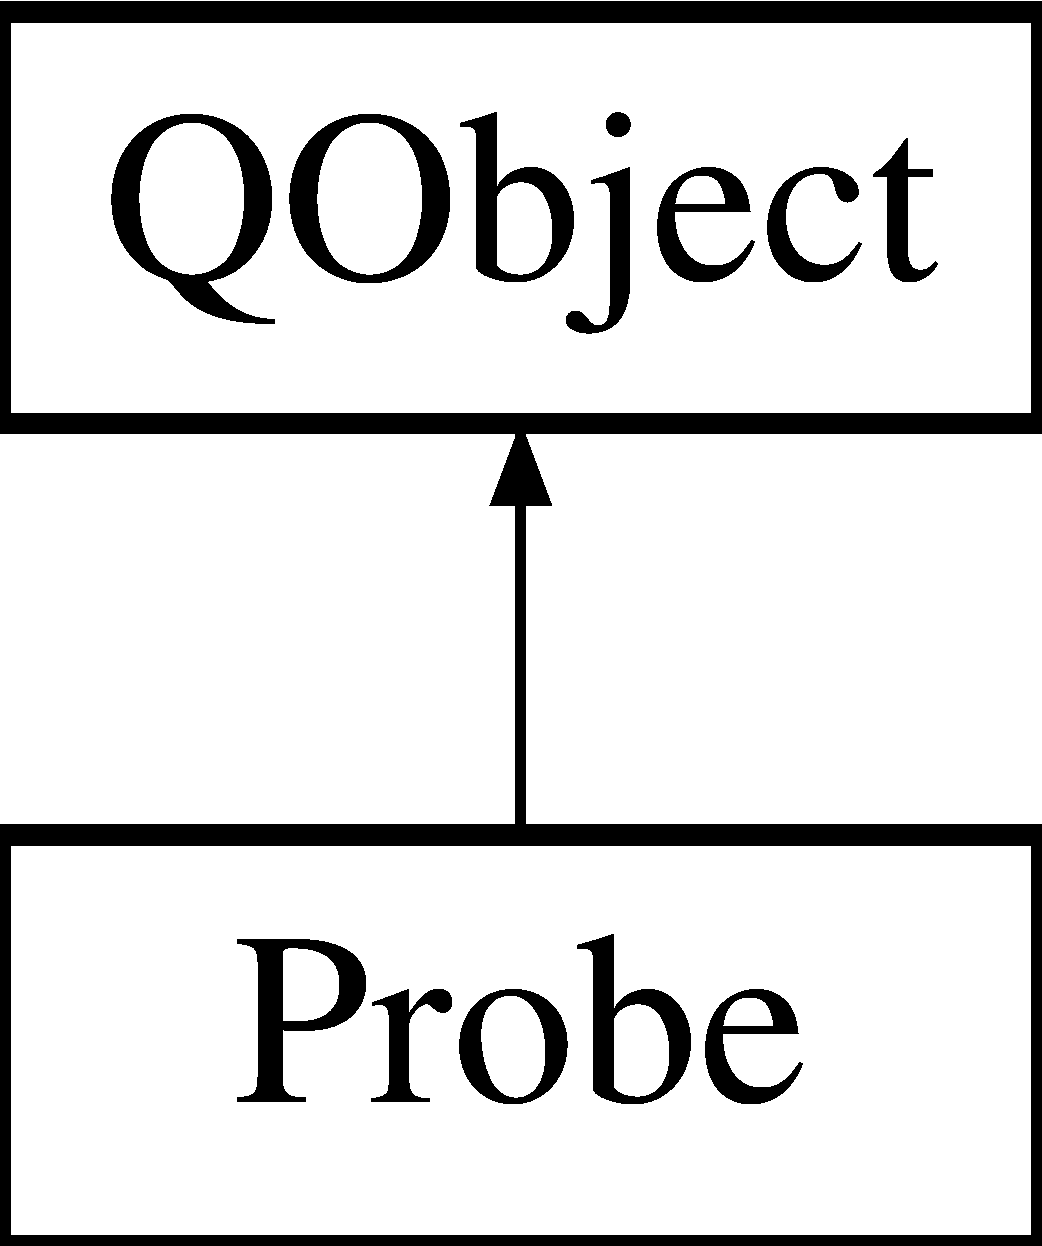
\includegraphics[height=2.000000cm]{class_probe}
\end{center}
\end{figure}
\subsection*{Public Member Functions}
\begin{DoxyCompactItemize}
\item 
\hyperlink{class_probe_a0c7c763cf0745c6a53cb1db579380e73}{Probe} (Q\+Object $\ast$parent)
\item 
\hyperlink{class_probe_a0bfeef911e78cd2ebc151da41a458f60}{$\sim$\+Probe} (void)
\item 
void \hyperlink{class_probe_add01ac928a09ba40f01bee3d2ffd8848}{set\+Position} (const Q\+Point \&\hyperlink{class_probe_afd206513c738cc239a95bad59445e998}{position})
\item 
void \hyperlink{class_probe_a00c9f00f28d8dd724ee21f9a4462e015}{set\+Color} (const Q\+Color \&\hyperlink{class_probe_a3b43c9b49f2672a7b0dd72bac25aab5c}{color})
\item 
void \hyperlink{class_probe_a1732d34c1e5b02e12b7ec405d144190f}{draw} ()
\item 
Q\+Color \hyperlink{class_probe_a3b43c9b49f2672a7b0dd72bac25aab5c}{color} () const 
\item 
Q\+Point \hyperlink{class_probe_afd206513c738cc239a95bad59445e998}{position} () const 
\item 
void \hyperlink{class_probe_a2cad80c5851ce1ab165f41e56075853d}{set\+Label} (const Q\+String \&tool\+Tip)
\item 
Q\+String \hyperlink{class_probe_aecea3294d0fc08031e3f4e58dc56e7fe}{label} () const 
\item 
void \hyperlink{class_probe_af03400f61740988afa1ea8de3c57b5a7}{hide} ()
\item 
void \hyperlink{class_probe_a740a926e11b7723f3069d163a0b44c57}{show} ()
\end{DoxyCompactItemize}
\subsection*{Public Attributes}
\begin{DoxyCompactItemize}
\item 
bool \hyperlink{class_probe_a70f4267a48449ffcaf533977713cf49c}{is\+Hidden}
\item 
\hyperlink{heart_defines_8h_a2f059cd81f362503874790462d535f5b}{C\+E\+L\+L\+\_\+\+T\+Y\+P\+E} \hyperlink{class_probe_a73c39e8dfc343d288a2590b4c14e358c}{type}
\item 
Q\+Point \hyperlink{class_probe_aec2e2de57497c0b53c150ec808089298}{my\+Position}
\end{DoxyCompactItemize}


\subsection{Constructor \& Destructor Documentation}
\hypertarget{class_probe_a0c7c763cf0745c6a53cb1db579380e73}{\index{Probe@{Probe}!Probe@{Probe}}
\index{Probe@{Probe}!Probe@{Probe}}
\subsubsection[{Probe}]{\setlength{\rightskip}{0pt plus 5cm}Probe\+::\+Probe (
\begin{DoxyParamCaption}
\item[{Q\+Object $\ast$}]{parent}
\end{DoxyParamCaption}
)}}\label{class_probe_a0c7c763cf0745c6a53cb1db579380e73}
\hypertarget{class_probe_a0bfeef911e78cd2ebc151da41a458f60}{\index{Probe@{Probe}!````~Probe@{$\sim$\+Probe}}
\index{````~Probe@{$\sim$\+Probe}!Probe@{Probe}}
\subsubsection[{$\sim$\+Probe}]{\setlength{\rightskip}{0pt plus 5cm}Probe\+::$\sim$\+Probe (
\begin{DoxyParamCaption}
\item[{void}]{}
\end{DoxyParamCaption}
)}}\label{class_probe_a0bfeef911e78cd2ebc151da41a458f60}


\subsection{Member Function Documentation}
\hypertarget{class_probe_a3b43c9b49f2672a7b0dd72bac25aab5c}{\index{Probe@{Probe}!color@{color}}
\index{color@{color}!Probe@{Probe}}
\subsubsection[{color}]{\setlength{\rightskip}{0pt plus 5cm}Q\+Color Probe\+::color (
\begin{DoxyParamCaption}
{}
\end{DoxyParamCaption}
) const}}\label{class_probe_a3b43c9b49f2672a7b0dd72bac25aab5c}
\hypertarget{class_probe_a1732d34c1e5b02e12b7ec405d144190f}{\index{Probe@{Probe}!draw@{draw}}
\index{draw@{draw}!Probe@{Probe}}
\subsubsection[{draw}]{\setlength{\rightskip}{0pt plus 5cm}void Probe\+::draw (
\begin{DoxyParamCaption}
{}
\end{DoxyParamCaption}
)}}\label{class_probe_a1732d34c1e5b02e12b7ec405d144190f}
\hypertarget{class_probe_af03400f61740988afa1ea8de3c57b5a7}{\index{Probe@{Probe}!hide@{hide}}
\index{hide@{hide}!Probe@{Probe}}
\subsubsection[{hide}]{\setlength{\rightskip}{0pt plus 5cm}void Probe\+::hide (
\begin{DoxyParamCaption}
{}
\end{DoxyParamCaption}
)}}\label{class_probe_af03400f61740988afa1ea8de3c57b5a7}
\hypertarget{class_probe_aecea3294d0fc08031e3f4e58dc56e7fe}{\index{Probe@{Probe}!label@{label}}
\index{label@{label}!Probe@{Probe}}
\subsubsection[{label}]{\setlength{\rightskip}{0pt plus 5cm}Q\+String Probe\+::label (
\begin{DoxyParamCaption}
{}
\end{DoxyParamCaption}
) const}}\label{class_probe_aecea3294d0fc08031e3f4e58dc56e7fe}
\hypertarget{class_probe_afd206513c738cc239a95bad59445e998}{\index{Probe@{Probe}!position@{position}}
\index{position@{position}!Probe@{Probe}}
\subsubsection[{position}]{\setlength{\rightskip}{0pt plus 5cm}Q\+Point Probe\+::position (
\begin{DoxyParamCaption}
{}
\end{DoxyParamCaption}
) const}}\label{class_probe_afd206513c738cc239a95bad59445e998}
\hypertarget{class_probe_a00c9f00f28d8dd724ee21f9a4462e015}{\index{Probe@{Probe}!set\+Color@{set\+Color}}
\index{set\+Color@{set\+Color}!Probe@{Probe}}
\subsubsection[{set\+Color}]{\setlength{\rightskip}{0pt plus 5cm}void Probe\+::set\+Color (
\begin{DoxyParamCaption}
\item[{const Q\+Color \&}]{color}
\end{DoxyParamCaption}
)}}\label{class_probe_a00c9f00f28d8dd724ee21f9a4462e015}
\hypertarget{class_probe_a2cad80c5851ce1ab165f41e56075853d}{\index{Probe@{Probe}!set\+Label@{set\+Label}}
\index{set\+Label@{set\+Label}!Probe@{Probe}}
\subsubsection[{set\+Label}]{\setlength{\rightskip}{0pt plus 5cm}void Probe\+::set\+Label (
\begin{DoxyParamCaption}
\item[{const Q\+String \&}]{tool\+Tip}
\end{DoxyParamCaption}
)}}\label{class_probe_a2cad80c5851ce1ab165f41e56075853d}
\hypertarget{class_probe_add01ac928a09ba40f01bee3d2ffd8848}{\index{Probe@{Probe}!set\+Position@{set\+Position}}
\index{set\+Position@{set\+Position}!Probe@{Probe}}
\subsubsection[{set\+Position}]{\setlength{\rightskip}{0pt plus 5cm}void Probe\+::set\+Position (
\begin{DoxyParamCaption}
\item[{const Q\+Point \&}]{position}
\end{DoxyParamCaption}
)}}\label{class_probe_add01ac928a09ba40f01bee3d2ffd8848}
\hypertarget{class_probe_a740a926e11b7723f3069d163a0b44c57}{\index{Probe@{Probe}!show@{show}}
\index{show@{show}!Probe@{Probe}}
\subsubsection[{show}]{\setlength{\rightskip}{0pt plus 5cm}void Probe\+::show (
\begin{DoxyParamCaption}
{}
\end{DoxyParamCaption}
)}}\label{class_probe_a740a926e11b7723f3069d163a0b44c57}


\subsection{Member Data Documentation}
\hypertarget{class_probe_a70f4267a48449ffcaf533977713cf49c}{\index{Probe@{Probe}!is\+Hidden@{is\+Hidden}}
\index{is\+Hidden@{is\+Hidden}!Probe@{Probe}}
\subsubsection[{is\+Hidden}]{\setlength{\rightskip}{0pt plus 5cm}bool Probe\+::is\+Hidden}}\label{class_probe_a70f4267a48449ffcaf533977713cf49c}
\hypertarget{class_probe_aec2e2de57497c0b53c150ec808089298}{\index{Probe@{Probe}!my\+Position@{my\+Position}}
\index{my\+Position@{my\+Position}!Probe@{Probe}}
\subsubsection[{my\+Position}]{\setlength{\rightskip}{0pt plus 5cm}Q\+Point Probe\+::my\+Position}}\label{class_probe_aec2e2de57497c0b53c150ec808089298}
\hypertarget{class_probe_a73c39e8dfc343d288a2590b4c14e358c}{\index{Probe@{Probe}!type@{type}}
\index{type@{type}!Probe@{Probe}}
\subsubsection[{type}]{\setlength{\rightskip}{0pt plus 5cm}{\bf C\+E\+L\+L\+\_\+\+T\+Y\+P\+E} Probe\+::type}}\label{class_probe_a73c39e8dfc343d288a2590b4c14e358c}


The documentation for this class was generated from the following files\+:\begin{DoxyCompactItemize}
\item 
\hyperlink{_probe_8h}{Probe.\+h}\item 
\hyperlink{_probe_8cpp}{Probe.\+cpp}\end{DoxyCompactItemize}

\hypertarget{class_random_generator}{\section{Random\+Generator Class Reference}
\label{class_random_generator}\index{Random\+Generator@{Random\+Generator}}
}


{\ttfamily \#include $<$Random\+Generator.\+h$>$}

\subsection*{Public Member Functions}
\begin{DoxyCompactItemize}
\item 
\hyperlink{class_random_generator_ad68dfb1d3d6164777c27beb1d5869873}{Random\+Generator} (void)
\item 
\hyperlink{class_random_generator_ada0252d5def711284f6b381a3aa85b6e}{$\sim$\+Random\+Generator} (void)
\item 
double \hyperlink{class_random_generator_a354e78930c8d4dd84dee041d8b5e3e2d}{gauss\+Function} (double y, double mean, double sigma)
\item 
double \hyperlink{class_random_generator_a89a28448defc23c508267db51bee1ba0}{gauss\+Random} (double mean, double sigma)
\item 
double \hyperlink{class_random_generator_a466cd9a5f2aba42f297fcd65b5ee2de9}{uniform} ()
\item 
int \hyperlink{class_random_generator_aeacd03768fb03aba8fbc34b1966ffbb2}{flipper} (int max\+Number)
\end{DoxyCompactItemize}


\subsection{Constructor \& Destructor Documentation}
\hypertarget{class_random_generator_ad68dfb1d3d6164777c27beb1d5869873}{\index{Random\+Generator@{Random\+Generator}!Random\+Generator@{Random\+Generator}}
\index{Random\+Generator@{Random\+Generator}!Random\+Generator@{Random\+Generator}}
\subsubsection[{Random\+Generator}]{\setlength{\rightskip}{0pt plus 5cm}Random\+Generator\+::\+Random\+Generator (
\begin{DoxyParamCaption}
\item[{void}]{}
\end{DoxyParamCaption}
)}}\label{class_random_generator_ad68dfb1d3d6164777c27beb1d5869873}
\hypertarget{class_random_generator_ada0252d5def711284f6b381a3aa85b6e}{\index{Random\+Generator@{Random\+Generator}!````~Random\+Generator@{$\sim$\+Random\+Generator}}
\index{````~Random\+Generator@{$\sim$\+Random\+Generator}!Random\+Generator@{Random\+Generator}}
\subsubsection[{$\sim$\+Random\+Generator}]{\setlength{\rightskip}{0pt plus 5cm}Random\+Generator\+::$\sim$\+Random\+Generator (
\begin{DoxyParamCaption}
\item[{void}]{}
\end{DoxyParamCaption}
)}}\label{class_random_generator_ada0252d5def711284f6b381a3aa85b6e}


\subsection{Member Function Documentation}
\hypertarget{class_random_generator_aeacd03768fb03aba8fbc34b1966ffbb2}{\index{Random\+Generator@{Random\+Generator}!flipper@{flipper}}
\index{flipper@{flipper}!Random\+Generator@{Random\+Generator}}
\subsubsection[{flipper}]{\setlength{\rightskip}{0pt plus 5cm}int Random\+Generator\+::flipper (
\begin{DoxyParamCaption}
\item[{int}]{max\+Number}
\end{DoxyParamCaption}
)}}\label{class_random_generator_aeacd03768fb03aba8fbc34b1966ffbb2}
\hypertarget{class_random_generator_a354e78930c8d4dd84dee041d8b5e3e2d}{\index{Random\+Generator@{Random\+Generator}!gauss\+Function@{gauss\+Function}}
\index{gauss\+Function@{gauss\+Function}!Random\+Generator@{Random\+Generator}}
\subsubsection[{gauss\+Function}]{\setlength{\rightskip}{0pt plus 5cm}double Random\+Generator\+::gauss\+Function (
\begin{DoxyParamCaption}
\item[{double}]{y, }
\item[{double}]{mean, }
\item[{double}]{sigma}
\end{DoxyParamCaption}
)}}\label{class_random_generator_a354e78930c8d4dd84dee041d8b5e3e2d}
\hypertarget{class_random_generator_a89a28448defc23c508267db51bee1ba0}{\index{Random\+Generator@{Random\+Generator}!gauss\+Random@{gauss\+Random}}
\index{gauss\+Random@{gauss\+Random}!Random\+Generator@{Random\+Generator}}
\subsubsection[{gauss\+Random}]{\setlength{\rightskip}{0pt plus 5cm}double Random\+Generator\+::gauss\+Random (
\begin{DoxyParamCaption}
\item[{double}]{mean, }
\item[{double}]{sigma}
\end{DoxyParamCaption}
)}}\label{class_random_generator_a89a28448defc23c508267db51bee1ba0}
\hypertarget{class_random_generator_a466cd9a5f2aba42f297fcd65b5ee2de9}{\index{Random\+Generator@{Random\+Generator}!uniform@{uniform}}
\index{uniform@{uniform}!Random\+Generator@{Random\+Generator}}
\subsubsection[{uniform}]{\setlength{\rightskip}{0pt plus 5cm}double Random\+Generator\+::uniform (
\begin{DoxyParamCaption}
{}
\end{DoxyParamCaption}
)}}\label{class_random_generator_a466cd9a5f2aba42f297fcd65b5ee2de9}


The documentation for this class was generated from the following files\+:\begin{DoxyCompactItemize}
\item 
\hyperlink{_random_generator_8h}{Random\+Generator.\+h}\item 
\hyperlink{_random_generator_8cpp}{Random\+Generator.\+cpp}\end{DoxyCompactItemize}

\hypertarget{class_r_rcalculator}{\section{R\+Rcalculator Class Reference}
\label{class_r_rcalculator}\index{R\+Rcalculator@{R\+Rcalculator}}
}


{\ttfamily \#include $<$R\+Rcalculator.\+h$>$}

Inheritance diagram for R\+Rcalculator\+:\begin{figure}[H]
\begin{center}
\leavevmode
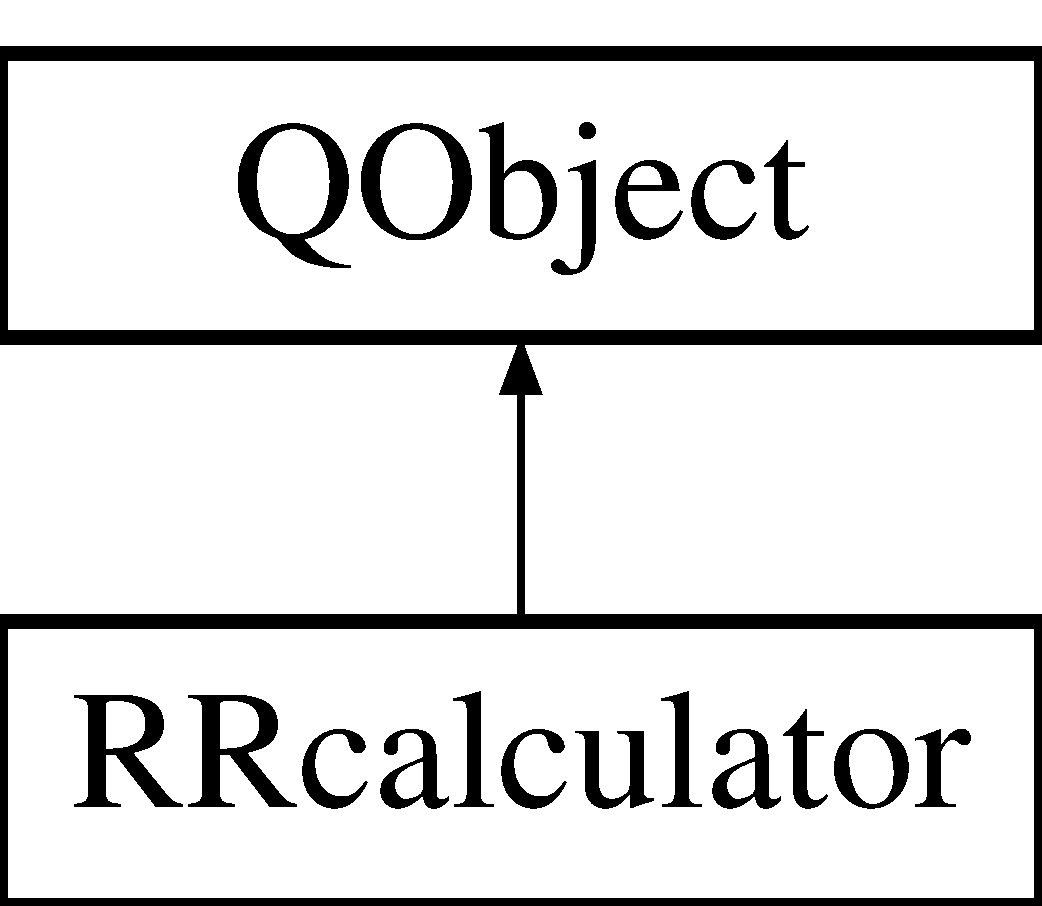
\includegraphics[height=2.000000cm]{class_r_rcalculator}
\end{center}
\end{figure}
\subsection*{Public Slots}
\begin{DoxyCompactItemize}
\item 
void \hyperlink{class_r_rcalculator_affa5d0f172be4d9aa0601c8f1824aba7}{reset} ()
\item 
void \hyperlink{class_r_rcalculator_a06b4c617afcb01dc74c6c542ede4af05}{process\+New\+Time} (double time, double potential)
\item 
void \hyperlink{class_r_rcalculator_a91d3f4c5a7a4ca1f749a9ecada0b7d5c}{calculate\+Pat\+En} (double rr)
\item 
void \hyperlink{class_r_rcalculator_ac55486650721726e4193bdc77b2f6bbe}{calculate\+Var\+En} (double rr)
\end{DoxyCompactItemize}
\subsection*{Signals}
\begin{DoxyCompactItemize}
\item 
void \hyperlink{class_r_rcalculator_aa8fa57e1512d3883d321a2d8a85151c3}{next\+R\+R} (double rr)
\item 
void \hyperlink{class_r_rcalculator_aa0c89346708b0ec0b64b4256a0120c1f}{cur\+Index} (int i)
\item 
void \hyperlink{class_r_rcalculator_a43e47f2cb76a4463da74deacabbafb12}{next\+Pat\+En} (double value)
\item 
void \hyperlink{class_r_rcalculator_a95e6ec7b23c518a8e381e3c0ae65b628}{next\+Var\+En} (double value)
\end{DoxyCompactItemize}
\subsection*{Public Member Functions}
\begin{DoxyCompactItemize}
\item 
void \hyperlink{class_r_rcalculator_ac612758f699b103d8deedf130dbc8cc9}{set\+Range\+Of\+Focus} (int range)
\item 
\hyperlink{class_r_rcalculator_a1c8424d714a284daa7a87f634b4f8c1e}{R\+Rcalculator} (\hyperlink{classatrial_parameters}{atrial\+Parameters} $\ast$definitions)
\item 
\hyperlink{class_r_rcalculator_a8af8b7c5cb9fd55b78757780ba8c3007}{$\sim$\+R\+Rcalculator} (void)
\end{DoxyCompactItemize}
\subsection*{Public Attributes}
\begin{DoxyCompactItemize}
\item 
std\+::vector$<$ double $>$ \hyperlink{class_r_rcalculator_a9c99b0abb14ec0a15edb6516202f1670}{intervals\+R\+R}
\item 
std\+::vector$<$ double $>$ \hyperlink{class_r_rcalculator_abb337d30cfd2d443d7aa00e62f8d12a0}{intervals\+Potential}
\item 
std\+::vector$<$ double $>$ \hyperlink{class_r_rcalculator_accf15b47a0f368de9dd5a1d758dac8a8}{intervals\+Saved}
\item 
std\+::vector$<$ double $>$ \hyperlink{class_r_rcalculator_ad7f152f6ec71894388eca83acce27c82}{m\+\_\+histogram}
\item 
std\+::vector$<$ double $>$ \hyperlink{class_r_rcalculator_a1a62706d3af65ec918550715e4748666}{m\+\_\+histogram\+\_\+0}
\item 
std\+::vector$<$ double $>$ \hyperlink{class_r_rcalculator_a88044253bb67963b690efe03b4566461}{m\+\_\+histogram\+\_\+1t}
\item 
std\+::vector$<$ double $>$ \hyperlink{class_r_rcalculator_a22fd8fedd28bf0b6455eb3a7ade48960}{m\+\_\+histogram\+\_\+2t}
\item 
double \hyperlink{class_r_rcalculator_ab2de224108c8ae0611b0a8b12cf9ce1f}{m\+\_\+pat\+En}
\item 
double \hyperlink{class_r_rcalculator_a94f0e6781def8bd5e38124e3144d3acc}{m\+\_\+var\+En}
\end{DoxyCompactItemize}


\subsection{Constructor \& Destructor Documentation}
\hypertarget{class_r_rcalculator_a1c8424d714a284daa7a87f634b4f8c1e}{\index{R\+Rcalculator@{R\+Rcalculator}!R\+Rcalculator@{R\+Rcalculator}}
\index{R\+Rcalculator@{R\+Rcalculator}!R\+Rcalculator@{R\+Rcalculator}}
\subsubsection[{R\+Rcalculator}]{\setlength{\rightskip}{0pt plus 5cm}R\+Rcalculator\+::\+R\+Rcalculator (
\begin{DoxyParamCaption}
\item[{{\bf atrial\+Parameters} $\ast$}]{definitions}
\end{DoxyParamCaption}
)}}\label{class_r_rcalculator_a1c8424d714a284daa7a87f634b4f8c1e}
\hypertarget{class_r_rcalculator_a8af8b7c5cb9fd55b78757780ba8c3007}{\index{R\+Rcalculator@{R\+Rcalculator}!````~R\+Rcalculator@{$\sim$\+R\+Rcalculator}}
\index{````~R\+Rcalculator@{$\sim$\+R\+Rcalculator}!R\+Rcalculator@{R\+Rcalculator}}
\subsubsection[{$\sim$\+R\+Rcalculator}]{\setlength{\rightskip}{0pt plus 5cm}R\+Rcalculator\+::$\sim$\+R\+Rcalculator (
\begin{DoxyParamCaption}
\item[{void}]{}
\end{DoxyParamCaption}
)}}\label{class_r_rcalculator_a8af8b7c5cb9fd55b78757780ba8c3007}


\subsection{Member Function Documentation}
\hypertarget{class_r_rcalculator_a91d3f4c5a7a4ca1f749a9ecada0b7d5c}{\index{R\+Rcalculator@{R\+Rcalculator}!calculate\+Pat\+En@{calculate\+Pat\+En}}
\index{calculate\+Pat\+En@{calculate\+Pat\+En}!R\+Rcalculator@{R\+Rcalculator}}
\subsubsection[{calculate\+Pat\+En}]{\setlength{\rightskip}{0pt plus 5cm}void R\+Rcalculator\+::calculate\+Pat\+En (
\begin{DoxyParamCaption}
\item[{double}]{rr}
\end{DoxyParamCaption}
)\hspace{0.3cm}{\ttfamily [slot]}}}\label{class_r_rcalculator_a91d3f4c5a7a4ca1f749a9ecada0b7d5c}
\hypertarget{class_r_rcalculator_ac55486650721726e4193bdc77b2f6bbe}{\index{R\+Rcalculator@{R\+Rcalculator}!calculate\+Var\+En@{calculate\+Var\+En}}
\index{calculate\+Var\+En@{calculate\+Var\+En}!R\+Rcalculator@{R\+Rcalculator}}
\subsubsection[{calculate\+Var\+En}]{\setlength{\rightskip}{0pt plus 5cm}void R\+Rcalculator\+::calculate\+Var\+En (
\begin{DoxyParamCaption}
\item[{double}]{rr}
\end{DoxyParamCaption}
)\hspace{0.3cm}{\ttfamily [slot]}}}\label{class_r_rcalculator_ac55486650721726e4193bdc77b2f6bbe}
\hypertarget{class_r_rcalculator_aa0c89346708b0ec0b64b4256a0120c1f}{\index{R\+Rcalculator@{R\+Rcalculator}!cur\+Index@{cur\+Index}}
\index{cur\+Index@{cur\+Index}!R\+Rcalculator@{R\+Rcalculator}}
\subsubsection[{cur\+Index}]{\setlength{\rightskip}{0pt plus 5cm}void R\+Rcalculator\+::cur\+Index (
\begin{DoxyParamCaption}
\item[{int}]{i}
\end{DoxyParamCaption}
)\hspace{0.3cm}{\ttfamily [signal]}}}\label{class_r_rcalculator_aa0c89346708b0ec0b64b4256a0120c1f}
\hypertarget{class_r_rcalculator_a43e47f2cb76a4463da74deacabbafb12}{\index{R\+Rcalculator@{R\+Rcalculator}!next\+Pat\+En@{next\+Pat\+En}}
\index{next\+Pat\+En@{next\+Pat\+En}!R\+Rcalculator@{R\+Rcalculator}}
\subsubsection[{next\+Pat\+En}]{\setlength{\rightskip}{0pt plus 5cm}void R\+Rcalculator\+::next\+Pat\+En (
\begin{DoxyParamCaption}
\item[{double}]{value}
\end{DoxyParamCaption}
)\hspace{0.3cm}{\ttfamily [signal]}}}\label{class_r_rcalculator_a43e47f2cb76a4463da74deacabbafb12}
\hypertarget{class_r_rcalculator_aa8fa57e1512d3883d321a2d8a85151c3}{\index{R\+Rcalculator@{R\+Rcalculator}!next\+R\+R@{next\+R\+R}}
\index{next\+R\+R@{next\+R\+R}!R\+Rcalculator@{R\+Rcalculator}}
\subsubsection[{next\+R\+R}]{\setlength{\rightskip}{0pt plus 5cm}void R\+Rcalculator\+::next\+R\+R (
\begin{DoxyParamCaption}
\item[{double}]{rr}
\end{DoxyParamCaption}
)\hspace{0.3cm}{\ttfamily [signal]}}}\label{class_r_rcalculator_aa8fa57e1512d3883d321a2d8a85151c3}
\hypertarget{class_r_rcalculator_a95e6ec7b23c518a8e381e3c0ae65b628}{\index{R\+Rcalculator@{R\+Rcalculator}!next\+Var\+En@{next\+Var\+En}}
\index{next\+Var\+En@{next\+Var\+En}!R\+Rcalculator@{R\+Rcalculator}}
\subsubsection[{next\+Var\+En}]{\setlength{\rightskip}{0pt plus 5cm}void R\+Rcalculator\+::next\+Var\+En (
\begin{DoxyParamCaption}
\item[{double}]{value}
\end{DoxyParamCaption}
)\hspace{0.3cm}{\ttfamily [signal]}}}\label{class_r_rcalculator_a95e6ec7b23c518a8e381e3c0ae65b628}
\hypertarget{class_r_rcalculator_a06b4c617afcb01dc74c6c542ede4af05}{\index{R\+Rcalculator@{R\+Rcalculator}!process\+New\+Time@{process\+New\+Time}}
\index{process\+New\+Time@{process\+New\+Time}!R\+Rcalculator@{R\+Rcalculator}}
\subsubsection[{process\+New\+Time}]{\setlength{\rightskip}{0pt plus 5cm}void R\+Rcalculator\+::process\+New\+Time (
\begin{DoxyParamCaption}
\item[{double}]{time, }
\item[{double}]{potential}
\end{DoxyParamCaption}
)\hspace{0.3cm}{\ttfamily [slot]}}}\label{class_r_rcalculator_a06b4c617afcb01dc74c6c542ede4af05}
\hypertarget{class_r_rcalculator_affa5d0f172be4d9aa0601c8f1824aba7}{\index{R\+Rcalculator@{R\+Rcalculator}!reset@{reset}}
\index{reset@{reset}!R\+Rcalculator@{R\+Rcalculator}}
\subsubsection[{reset}]{\setlength{\rightskip}{0pt plus 5cm}void R\+Rcalculator\+::reset (
\begin{DoxyParamCaption}
{}
\end{DoxyParamCaption}
)\hspace{0.3cm}{\ttfamily [slot]}}}\label{class_r_rcalculator_affa5d0f172be4d9aa0601c8f1824aba7}
\hypertarget{class_r_rcalculator_ac612758f699b103d8deedf130dbc8cc9}{\index{R\+Rcalculator@{R\+Rcalculator}!set\+Range\+Of\+Focus@{set\+Range\+Of\+Focus}}
\index{set\+Range\+Of\+Focus@{set\+Range\+Of\+Focus}!R\+Rcalculator@{R\+Rcalculator}}
\subsubsection[{set\+Range\+Of\+Focus}]{\setlength{\rightskip}{0pt plus 5cm}void R\+Rcalculator\+::set\+Range\+Of\+Focus (
\begin{DoxyParamCaption}
\item[{int}]{range}
\end{DoxyParamCaption}
)}}\label{class_r_rcalculator_ac612758f699b103d8deedf130dbc8cc9}


\subsection{Member Data Documentation}
\hypertarget{class_r_rcalculator_abb337d30cfd2d443d7aa00e62f8d12a0}{\index{R\+Rcalculator@{R\+Rcalculator}!intervals\+Potential@{intervals\+Potential}}
\index{intervals\+Potential@{intervals\+Potential}!R\+Rcalculator@{R\+Rcalculator}}
\subsubsection[{intervals\+Potential}]{\setlength{\rightskip}{0pt plus 5cm}std\+::vector$<$double$>$ R\+Rcalculator\+::intervals\+Potential}}\label{class_r_rcalculator_abb337d30cfd2d443d7aa00e62f8d12a0}
\hypertarget{class_r_rcalculator_a9c99b0abb14ec0a15edb6516202f1670}{\index{R\+Rcalculator@{R\+Rcalculator}!intervals\+R\+R@{intervals\+R\+R}}
\index{intervals\+R\+R@{intervals\+R\+R}!R\+Rcalculator@{R\+Rcalculator}}
\subsubsection[{intervals\+R\+R}]{\setlength{\rightskip}{0pt plus 5cm}std\+::vector$<$double$>$ R\+Rcalculator\+::intervals\+R\+R}}\label{class_r_rcalculator_a9c99b0abb14ec0a15edb6516202f1670}
\hypertarget{class_r_rcalculator_accf15b47a0f368de9dd5a1d758dac8a8}{\index{R\+Rcalculator@{R\+Rcalculator}!intervals\+Saved@{intervals\+Saved}}
\index{intervals\+Saved@{intervals\+Saved}!R\+Rcalculator@{R\+Rcalculator}}
\subsubsection[{intervals\+Saved}]{\setlength{\rightskip}{0pt plus 5cm}std\+::vector$<$double$>$ R\+Rcalculator\+::intervals\+Saved}}\label{class_r_rcalculator_accf15b47a0f368de9dd5a1d758dac8a8}
\hypertarget{class_r_rcalculator_ad7f152f6ec71894388eca83acce27c82}{\index{R\+Rcalculator@{R\+Rcalculator}!m\+\_\+histogram@{m\+\_\+histogram}}
\index{m\+\_\+histogram@{m\+\_\+histogram}!R\+Rcalculator@{R\+Rcalculator}}
\subsubsection[{m\+\_\+histogram}]{\setlength{\rightskip}{0pt plus 5cm}std\+::vector$<$double$>$ R\+Rcalculator\+::m\+\_\+histogram}}\label{class_r_rcalculator_ad7f152f6ec71894388eca83acce27c82}
\hypertarget{class_r_rcalculator_a1a62706d3af65ec918550715e4748666}{\index{R\+Rcalculator@{R\+Rcalculator}!m\+\_\+histogram\+\_\+0@{m\+\_\+histogram\+\_\+0}}
\index{m\+\_\+histogram\+\_\+0@{m\+\_\+histogram\+\_\+0}!R\+Rcalculator@{R\+Rcalculator}}
\subsubsection[{m\+\_\+histogram\+\_\+0}]{\setlength{\rightskip}{0pt plus 5cm}std\+::vector$<$double$>$ R\+Rcalculator\+::m\+\_\+histogram\+\_\+0}}\label{class_r_rcalculator_a1a62706d3af65ec918550715e4748666}
\hypertarget{class_r_rcalculator_a88044253bb67963b690efe03b4566461}{\index{R\+Rcalculator@{R\+Rcalculator}!m\+\_\+histogram\+\_\+1t@{m\+\_\+histogram\+\_\+1t}}
\index{m\+\_\+histogram\+\_\+1t@{m\+\_\+histogram\+\_\+1t}!R\+Rcalculator@{R\+Rcalculator}}
\subsubsection[{m\+\_\+histogram\+\_\+1t}]{\setlength{\rightskip}{0pt plus 5cm}std\+::vector$<$double$>$ R\+Rcalculator\+::m\+\_\+histogram\+\_\+1t}}\label{class_r_rcalculator_a88044253bb67963b690efe03b4566461}
\hypertarget{class_r_rcalculator_a22fd8fedd28bf0b6455eb3a7ade48960}{\index{R\+Rcalculator@{R\+Rcalculator}!m\+\_\+histogram\+\_\+2t@{m\+\_\+histogram\+\_\+2t}}
\index{m\+\_\+histogram\+\_\+2t@{m\+\_\+histogram\+\_\+2t}!R\+Rcalculator@{R\+Rcalculator}}
\subsubsection[{m\+\_\+histogram\+\_\+2t}]{\setlength{\rightskip}{0pt plus 5cm}std\+::vector$<$double$>$ R\+Rcalculator\+::m\+\_\+histogram\+\_\+2t}}\label{class_r_rcalculator_a22fd8fedd28bf0b6455eb3a7ade48960}
\hypertarget{class_r_rcalculator_ab2de224108c8ae0611b0a8b12cf9ce1f}{\index{R\+Rcalculator@{R\+Rcalculator}!m\+\_\+pat\+En@{m\+\_\+pat\+En}}
\index{m\+\_\+pat\+En@{m\+\_\+pat\+En}!R\+Rcalculator@{R\+Rcalculator}}
\subsubsection[{m\+\_\+pat\+En}]{\setlength{\rightskip}{0pt plus 5cm}double R\+Rcalculator\+::m\+\_\+pat\+En}}\label{class_r_rcalculator_ab2de224108c8ae0611b0a8b12cf9ce1f}
\hypertarget{class_r_rcalculator_a94f0e6781def8bd5e38124e3144d3acc}{\index{R\+Rcalculator@{R\+Rcalculator}!m\+\_\+var\+En@{m\+\_\+var\+En}}
\index{m\+\_\+var\+En@{m\+\_\+var\+En}!R\+Rcalculator@{R\+Rcalculator}}
\subsubsection[{m\+\_\+var\+En}]{\setlength{\rightskip}{0pt plus 5cm}double R\+Rcalculator\+::m\+\_\+var\+En}}\label{class_r_rcalculator_a94f0e6781def8bd5e38124e3144d3acc}


The documentation for this class was generated from the following files\+:\begin{DoxyCompactItemize}
\item 
\hyperlink{_r_rcalculator_8h}{R\+Rcalculator.\+h}\item 
\hyperlink{_r_rcalculator_8cpp}{R\+Rcalculator.\+cpp}\end{DoxyCompactItemize}

\hypertarget{classrr_plot}{\section{rr\+Plot Class Reference}
\label{classrr_plot}\index{rr\+Plot@{rr\+Plot}}
}


{\ttfamily \#include $<$rr\+Plot.\+h$>$}

Inheritance diagram for rr\+Plot\+:\begin{figure}[H]
\begin{center}
\leavevmode
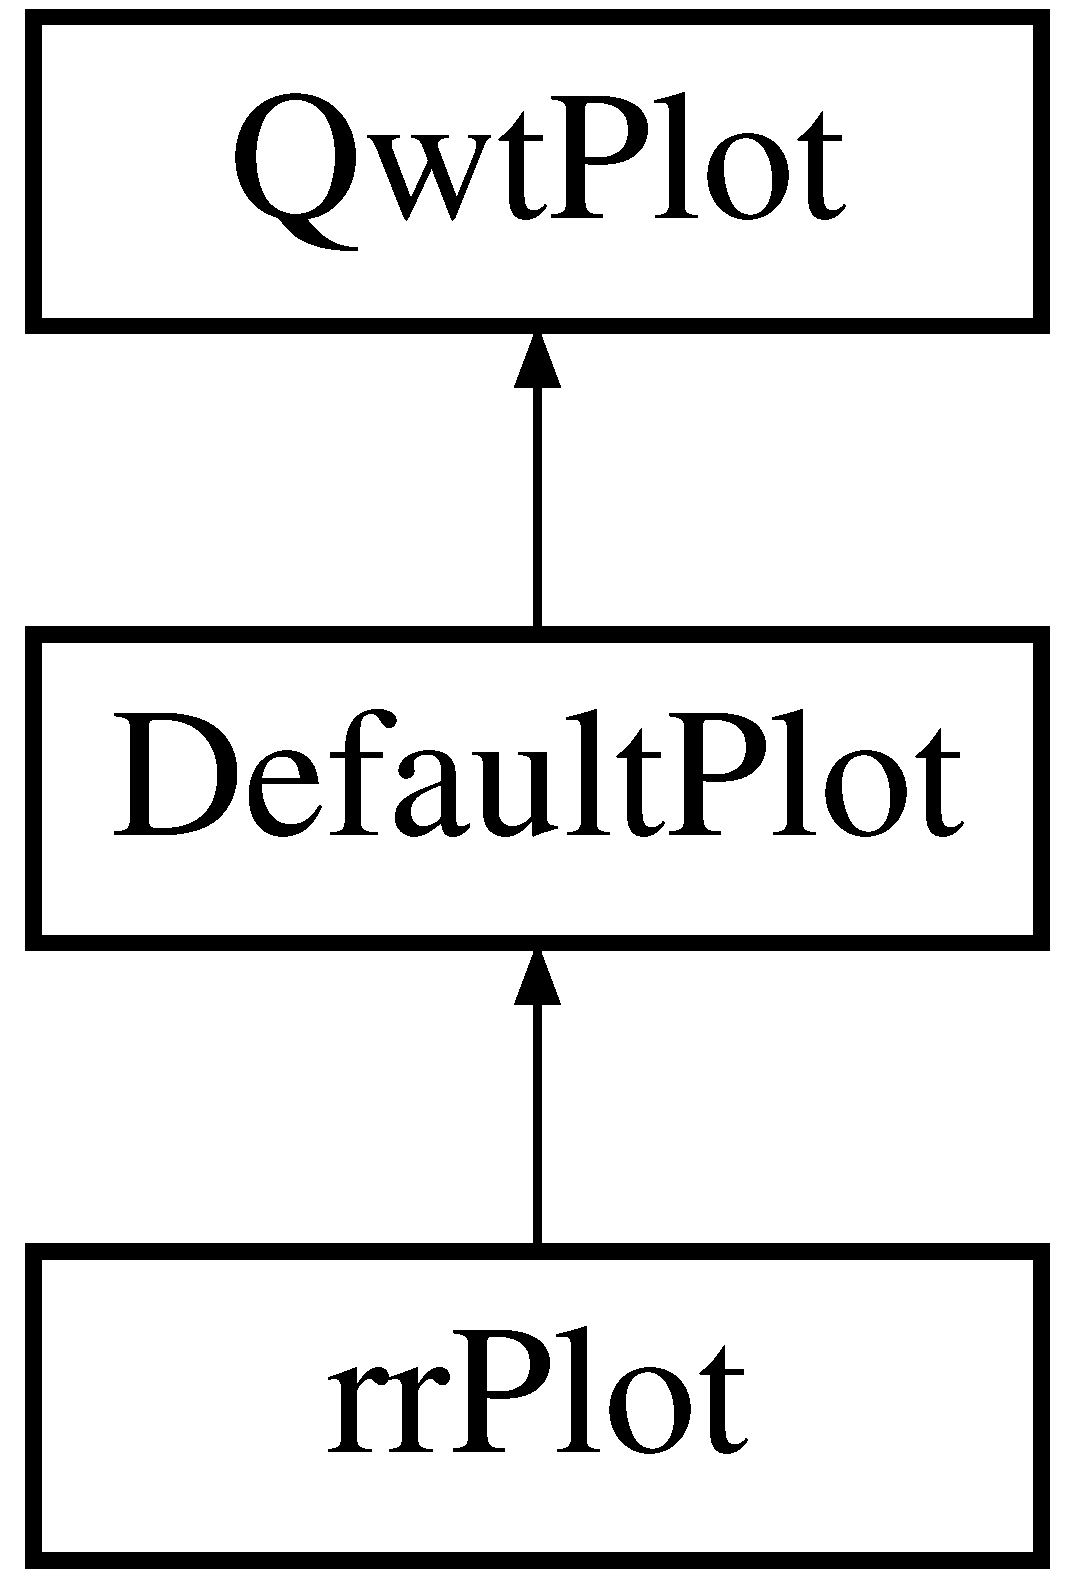
\includegraphics[height=3.000000cm]{classrr_plot}
\end{center}
\end{figure}
\subsection*{Public Slots}
\begin{DoxyCompactItemize}
\item 
void \hyperlink{classrr_plot_ae2dd42e0e8f94bc4b1f9b4bc5e917bcb}{append\+R\+R} (double y)
\item 
void \hyperlink{classrr_plot_a4330236961be8adaf9fb44ce45b5b63a}{pane\+Left} ()
\item 
void \hyperlink{classrr_plot_a1294ab460597423936b3e07bc009c174}{pane\+Right} ()
\item 
void \hyperlink{classrr_plot_aa967ef18a8edb8ecd196198f10ecb97c}{clear} ()
\item 
void \hyperlink{classrr_plot_a9f78ddedf799bbe3cd8aa5cc1dbabd77}{pane\+Up} ()
\item 
void \hyperlink{classrr_plot_aeff81faaf8baf44874d58796298f2643}{pane\+Down} ()
\item 
void \hyperlink{classrr_plot_a6a5832444faeae2ec648cf512f44c66d}{zoom\+In\+X} ()
\item 
void \hyperlink{classrr_plot_a7c31bb252d002579c04a8038370685d7}{zoom\+Out\+X} ()
\item 
void \hyperlink{classrr_plot_a368f1da9929e078f53a1195fe54eaa56}{zoom\+In\+Y} ()
\item 
void \hyperlink{classrr_plot_a884169d9fccdd99d51f354d53fa3f1ab}{zoom\+Out\+Y} ()
\item 
void \hyperlink{classrr_plot_a69724f1f3c7623d83a599a86c6036261}{set\+Xmin} (double value)
\item 
void \hyperlink{classrr_plot_adf7f0349309cc79fcc6613fdb6613961}{set\+Xmax} (double value)
\item 
void \hyperlink{classrr_plot_a7254d3098b111df47e9d9e0ba3fe7dfd}{set\+Ymin} (double value)
\item 
void \hyperlink{classrr_plot_af85cc052d86396309c0eae44543f8c1b}{set\+Ymax} (double value)
\item 
void \hyperlink{classrr_plot_a744a715c88372fcf875370a213255d34}{autoscale} ()
\item 
void \hyperlink{classrr_plot_aeda7c441255d2d644222997b268d600e}{mouse\+Press\+Event} (Q\+Mouse\+Event $\ast$event)
\end{DoxyCompactItemize}
\subsection*{Public Member Functions}
\begin{DoxyCompactItemize}
\item 
\hyperlink{classrr_plot_a1670fc13172e2a65ed9c10fe2c65f53a}{rr\+Plot} (Q\+Widget $\ast$parent)
\item 
virtual \hyperlink{classrr_plot_a4804c1ab8d3cc373b8e12d660ea2dba6}{$\sim$rr\+Plot} ()
\end{DoxyCompactItemize}
\subsection*{Public Attributes}
\begin{DoxyCompactItemize}
\item 
double \hyperlink{classrr_plot_aa21b657663077f2bc1a43e630685906b}{scale\+\_\+\+Yd}
\item 
double \hyperlink{classrr_plot_a9c714381d88800087dea02cc188aed89}{scale\+\_\+\+Yu}
\end{DoxyCompactItemize}
\subsection*{Additional Inherited Members}


\subsection{Constructor \& Destructor Documentation}
\hypertarget{classrr_plot_a1670fc13172e2a65ed9c10fe2c65f53a}{\index{rr\+Plot@{rr\+Plot}!rr\+Plot@{rr\+Plot}}
\index{rr\+Plot@{rr\+Plot}!rr\+Plot@{rr\+Plot}}
\subsubsection[{rr\+Plot}]{\setlength{\rightskip}{0pt plus 5cm}rr\+Plot\+::rr\+Plot (
\begin{DoxyParamCaption}
\item[{Q\+Widget $\ast$}]{parent}
\end{DoxyParamCaption}
)}}\label{classrr_plot_a1670fc13172e2a65ed9c10fe2c65f53a}
\hypertarget{classrr_plot_a4804c1ab8d3cc373b8e12d660ea2dba6}{\index{rr\+Plot@{rr\+Plot}!````~rr\+Plot@{$\sim$rr\+Plot}}
\index{````~rr\+Plot@{$\sim$rr\+Plot}!rr\+Plot@{rr\+Plot}}
\subsubsection[{$\sim$rr\+Plot}]{\setlength{\rightskip}{0pt plus 5cm}rr\+Plot\+::$\sim$rr\+Plot (
\begin{DoxyParamCaption}
\item[{void}]{}
\end{DoxyParamCaption}
)\hspace{0.3cm}{\ttfamily [virtual]}}}\label{classrr_plot_a4804c1ab8d3cc373b8e12d660ea2dba6}


\subsection{Member Function Documentation}
\hypertarget{classrr_plot_ae2dd42e0e8f94bc4b1f9b4bc5e917bcb}{\index{rr\+Plot@{rr\+Plot}!append\+R\+R@{append\+R\+R}}
\index{append\+R\+R@{append\+R\+R}!rr\+Plot@{rr\+Plot}}
\subsubsection[{append\+R\+R}]{\setlength{\rightskip}{0pt plus 5cm}void rr\+Plot\+::append\+R\+R (
\begin{DoxyParamCaption}
\item[{double}]{y}
\end{DoxyParamCaption}
)\hspace{0.3cm}{\ttfamily [slot]}}}\label{classrr_plot_ae2dd42e0e8f94bc4b1f9b4bc5e917bcb}
\hypertarget{classrr_plot_a744a715c88372fcf875370a213255d34}{\index{rr\+Plot@{rr\+Plot}!autoscale@{autoscale}}
\index{autoscale@{autoscale}!rr\+Plot@{rr\+Plot}}
\subsubsection[{autoscale}]{\setlength{\rightskip}{0pt plus 5cm}void rr\+Plot\+::autoscale (
\begin{DoxyParamCaption}
{}
\end{DoxyParamCaption}
)\hspace{0.3cm}{\ttfamily [slot]}}}\label{classrr_plot_a744a715c88372fcf875370a213255d34}
\hypertarget{classrr_plot_aa967ef18a8edb8ecd196198f10ecb97c}{\index{rr\+Plot@{rr\+Plot}!clear@{clear}}
\index{clear@{clear}!rr\+Plot@{rr\+Plot}}
\subsubsection[{clear}]{\setlength{\rightskip}{0pt plus 5cm}void rr\+Plot\+::clear (
\begin{DoxyParamCaption}
{}
\end{DoxyParamCaption}
)\hspace{0.3cm}{\ttfamily [slot]}}}\label{classrr_plot_aa967ef18a8edb8ecd196198f10ecb97c}
\hypertarget{classrr_plot_aeda7c441255d2d644222997b268d600e}{\index{rr\+Plot@{rr\+Plot}!mouse\+Press\+Event@{mouse\+Press\+Event}}
\index{mouse\+Press\+Event@{mouse\+Press\+Event}!rr\+Plot@{rr\+Plot}}
\subsubsection[{mouse\+Press\+Event}]{\setlength{\rightskip}{0pt plus 5cm}void rr\+Plot\+::mouse\+Press\+Event (
\begin{DoxyParamCaption}
\item[{Q\+Mouse\+Event $\ast$}]{event}
\end{DoxyParamCaption}
)\hspace{0.3cm}{\ttfamily [slot]}}}\label{classrr_plot_aeda7c441255d2d644222997b268d600e}
\hypertarget{classrr_plot_aeff81faaf8baf44874d58796298f2643}{\index{rr\+Plot@{rr\+Plot}!pane\+Down@{pane\+Down}}
\index{pane\+Down@{pane\+Down}!rr\+Plot@{rr\+Plot}}
\subsubsection[{pane\+Down}]{\setlength{\rightskip}{0pt plus 5cm}void rr\+Plot\+::pane\+Down (
\begin{DoxyParamCaption}
{}
\end{DoxyParamCaption}
)\hspace{0.3cm}{\ttfamily [slot]}}}\label{classrr_plot_aeff81faaf8baf44874d58796298f2643}
\hypertarget{classrr_plot_a4330236961be8adaf9fb44ce45b5b63a}{\index{rr\+Plot@{rr\+Plot}!pane\+Left@{pane\+Left}}
\index{pane\+Left@{pane\+Left}!rr\+Plot@{rr\+Plot}}
\subsubsection[{pane\+Left}]{\setlength{\rightskip}{0pt plus 5cm}void rr\+Plot\+::pane\+Left (
\begin{DoxyParamCaption}
{}
\end{DoxyParamCaption}
)\hspace{0.3cm}{\ttfamily [slot]}}}\label{classrr_plot_a4330236961be8adaf9fb44ce45b5b63a}
\hypertarget{classrr_plot_a1294ab460597423936b3e07bc009c174}{\index{rr\+Plot@{rr\+Plot}!pane\+Right@{pane\+Right}}
\index{pane\+Right@{pane\+Right}!rr\+Plot@{rr\+Plot}}
\subsubsection[{pane\+Right}]{\setlength{\rightskip}{0pt plus 5cm}void rr\+Plot\+::pane\+Right (
\begin{DoxyParamCaption}
{}
\end{DoxyParamCaption}
)\hspace{0.3cm}{\ttfamily [slot]}}}\label{classrr_plot_a1294ab460597423936b3e07bc009c174}
\hypertarget{classrr_plot_a9f78ddedf799bbe3cd8aa5cc1dbabd77}{\index{rr\+Plot@{rr\+Plot}!pane\+Up@{pane\+Up}}
\index{pane\+Up@{pane\+Up}!rr\+Plot@{rr\+Plot}}
\subsubsection[{pane\+Up}]{\setlength{\rightskip}{0pt plus 5cm}void rr\+Plot\+::pane\+Up (
\begin{DoxyParamCaption}
{}
\end{DoxyParamCaption}
)\hspace{0.3cm}{\ttfamily [slot]}}}\label{classrr_plot_a9f78ddedf799bbe3cd8aa5cc1dbabd77}
\hypertarget{classrr_plot_adf7f0349309cc79fcc6613fdb6613961}{\index{rr\+Plot@{rr\+Plot}!set\+Xmax@{set\+Xmax}}
\index{set\+Xmax@{set\+Xmax}!rr\+Plot@{rr\+Plot}}
\subsubsection[{set\+Xmax}]{\setlength{\rightskip}{0pt plus 5cm}void rr\+Plot\+::set\+Xmax (
\begin{DoxyParamCaption}
\item[{double}]{value}
\end{DoxyParamCaption}
)\hspace{0.3cm}{\ttfamily [slot]}}}\label{classrr_plot_adf7f0349309cc79fcc6613fdb6613961}
\hypertarget{classrr_plot_a69724f1f3c7623d83a599a86c6036261}{\index{rr\+Plot@{rr\+Plot}!set\+Xmin@{set\+Xmin}}
\index{set\+Xmin@{set\+Xmin}!rr\+Plot@{rr\+Plot}}
\subsubsection[{set\+Xmin}]{\setlength{\rightskip}{0pt plus 5cm}void rr\+Plot\+::set\+Xmin (
\begin{DoxyParamCaption}
\item[{double}]{value}
\end{DoxyParamCaption}
)\hspace{0.3cm}{\ttfamily [slot]}}}\label{classrr_plot_a69724f1f3c7623d83a599a86c6036261}
\hypertarget{classrr_plot_af85cc052d86396309c0eae44543f8c1b}{\index{rr\+Plot@{rr\+Plot}!set\+Ymax@{set\+Ymax}}
\index{set\+Ymax@{set\+Ymax}!rr\+Plot@{rr\+Plot}}
\subsubsection[{set\+Ymax}]{\setlength{\rightskip}{0pt plus 5cm}void rr\+Plot\+::set\+Ymax (
\begin{DoxyParamCaption}
\item[{double}]{value}
\end{DoxyParamCaption}
)\hspace{0.3cm}{\ttfamily [slot]}}}\label{classrr_plot_af85cc052d86396309c0eae44543f8c1b}
\hypertarget{classrr_plot_a7254d3098b111df47e9d9e0ba3fe7dfd}{\index{rr\+Plot@{rr\+Plot}!set\+Ymin@{set\+Ymin}}
\index{set\+Ymin@{set\+Ymin}!rr\+Plot@{rr\+Plot}}
\subsubsection[{set\+Ymin}]{\setlength{\rightskip}{0pt plus 5cm}void rr\+Plot\+::set\+Ymin (
\begin{DoxyParamCaption}
\item[{double}]{value}
\end{DoxyParamCaption}
)\hspace{0.3cm}{\ttfamily [slot]}}}\label{classrr_plot_a7254d3098b111df47e9d9e0ba3fe7dfd}
\hypertarget{classrr_plot_a6a5832444faeae2ec648cf512f44c66d}{\index{rr\+Plot@{rr\+Plot}!zoom\+In\+X@{zoom\+In\+X}}
\index{zoom\+In\+X@{zoom\+In\+X}!rr\+Plot@{rr\+Plot}}
\subsubsection[{zoom\+In\+X}]{\setlength{\rightskip}{0pt plus 5cm}void rr\+Plot\+::zoom\+In\+X (
\begin{DoxyParamCaption}
{}
\end{DoxyParamCaption}
)\hspace{0.3cm}{\ttfamily [slot]}}}\label{classrr_plot_a6a5832444faeae2ec648cf512f44c66d}
\hypertarget{classrr_plot_a368f1da9929e078f53a1195fe54eaa56}{\index{rr\+Plot@{rr\+Plot}!zoom\+In\+Y@{zoom\+In\+Y}}
\index{zoom\+In\+Y@{zoom\+In\+Y}!rr\+Plot@{rr\+Plot}}
\subsubsection[{zoom\+In\+Y}]{\setlength{\rightskip}{0pt plus 5cm}void rr\+Plot\+::zoom\+In\+Y (
\begin{DoxyParamCaption}
{}
\end{DoxyParamCaption}
)\hspace{0.3cm}{\ttfamily [slot]}}}\label{classrr_plot_a368f1da9929e078f53a1195fe54eaa56}
\hypertarget{classrr_plot_a7c31bb252d002579c04a8038370685d7}{\index{rr\+Plot@{rr\+Plot}!zoom\+Out\+X@{zoom\+Out\+X}}
\index{zoom\+Out\+X@{zoom\+Out\+X}!rr\+Plot@{rr\+Plot}}
\subsubsection[{zoom\+Out\+X}]{\setlength{\rightskip}{0pt plus 5cm}void rr\+Plot\+::zoom\+Out\+X (
\begin{DoxyParamCaption}
{}
\end{DoxyParamCaption}
)\hspace{0.3cm}{\ttfamily [slot]}}}\label{classrr_plot_a7c31bb252d002579c04a8038370685d7}
\hypertarget{classrr_plot_a884169d9fccdd99d51f354d53fa3f1ab}{\index{rr\+Plot@{rr\+Plot}!zoom\+Out\+Y@{zoom\+Out\+Y}}
\index{zoom\+Out\+Y@{zoom\+Out\+Y}!rr\+Plot@{rr\+Plot}}
\subsubsection[{zoom\+Out\+Y}]{\setlength{\rightskip}{0pt plus 5cm}void rr\+Plot\+::zoom\+Out\+Y (
\begin{DoxyParamCaption}
{}
\end{DoxyParamCaption}
)\hspace{0.3cm}{\ttfamily [slot]}}}\label{classrr_plot_a884169d9fccdd99d51f354d53fa3f1ab}


\subsection{Member Data Documentation}
\hypertarget{classrr_plot_aa21b657663077f2bc1a43e630685906b}{\index{rr\+Plot@{rr\+Plot}!scale\+\_\+\+Yd@{scale\+\_\+\+Yd}}
\index{scale\+\_\+\+Yd@{scale\+\_\+\+Yd}!rr\+Plot@{rr\+Plot}}
\subsubsection[{scale\+\_\+\+Yd}]{\setlength{\rightskip}{0pt plus 5cm}double rr\+Plot\+::scale\+\_\+\+Yd}}\label{classrr_plot_aa21b657663077f2bc1a43e630685906b}
\hypertarget{classrr_plot_a9c714381d88800087dea02cc188aed89}{\index{rr\+Plot@{rr\+Plot}!scale\+\_\+\+Yu@{scale\+\_\+\+Yu}}
\index{scale\+\_\+\+Yu@{scale\+\_\+\+Yu}!rr\+Plot@{rr\+Plot}}
\subsubsection[{scale\+\_\+\+Yu}]{\setlength{\rightskip}{0pt plus 5cm}double rr\+Plot\+::scale\+\_\+\+Yu}}\label{classrr_plot_a9c714381d88800087dea02cc188aed89}


The documentation for this class was generated from the following files\+:\begin{DoxyCompactItemize}
\item 
\hyperlink{rr_plot_8h}{rr\+Plot.\+h}\item 
\hyperlink{rr_plot_8cpp}{rr\+Plot.\+cpp}\end{DoxyCompactItemize}

\hypertarget{class_simple_heart}{\section{Simple\+Heart Class Reference}
\label{class_simple_heart}\index{Simple\+Heart@{Simple\+Heart}}
}


{\ttfamily \#include $<$simpleheart.\+h$>$}

Inheritance diagram for Simple\+Heart\+:\begin{figure}[H]
\begin{center}
\leavevmode
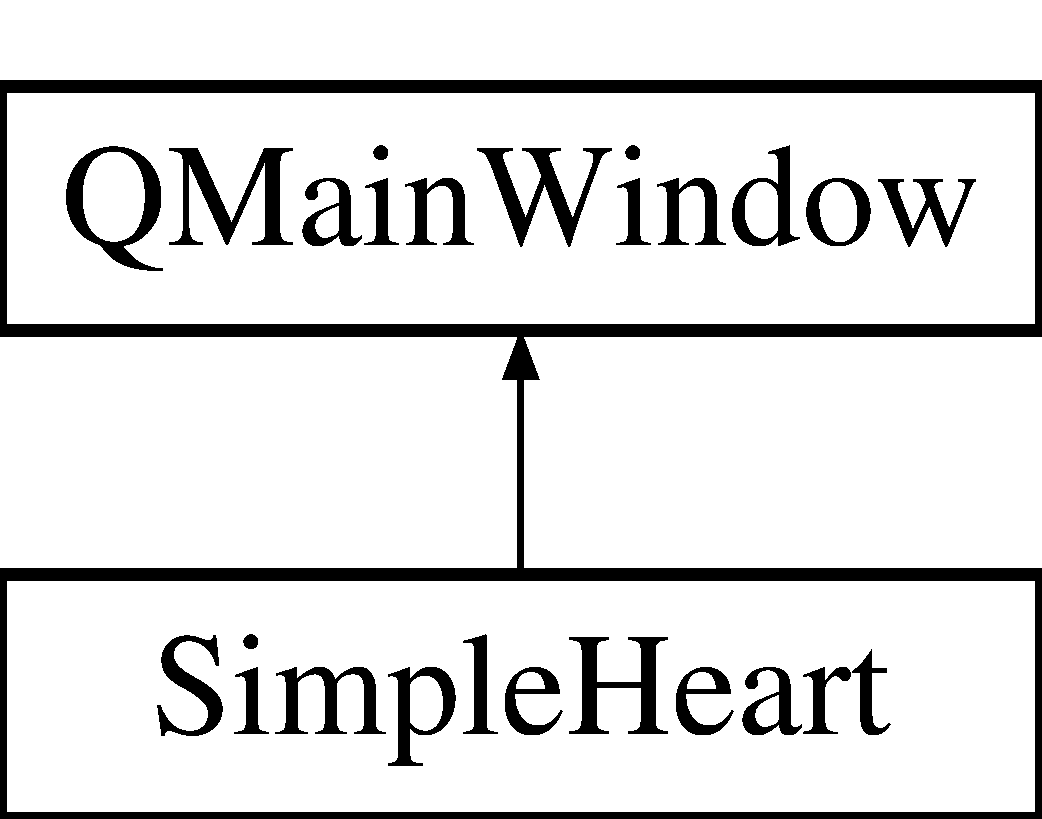
\includegraphics[height=2.000000cm]{class_simple_heart}
\end{center}
\end{figure}
\subsection*{Public Slots}
\begin{DoxyCompactItemize}
\item 
void \hyperlink{class_simple_heart_aff7605e57db713a7f55ca1b161ba524b}{reset} ()
\item 
void \hyperlink{class_simple_heart_ad5519be4fe9004e2726208111b294f0b}{set\+Timer\+Interval} (double interval)
\item 
void \hyperlink{class_simple_heart_a4ffc946d90c553de0fc523d955555f65}{stop\+Calculation} ()
\item 
void \hyperlink{class_simple_heart_a49deb5c528545bab494fd64069103480}{start\+Calculation} ()
\item 
void \hyperlink{class_simple_heart_a7518755827922e9a3fa12c3e2438b3de}{set\+State} (int val)
\item 
void \hyperlink{class_simple_heart_a9f8cc5db506750cc418f42af3c44d44e}{set\+Free\+Touch} (bool val)
\item 
void \hyperlink{class_simple_heart_abaf4c1874fa254d5a1c479d9c7a8dee4}{open\+Instruction} ()
\item 
void \hyperlink{class_simple_heart_a6bbe8cde23ba17c810fa0dbb1d6bd5bb}{open\+Settings} ()
\item 
void \hyperlink{class_simple_heart_a247bb22f52da28f0651973c103b79998}{reset\+Diffusion} ()
\item 
void \hyperlink{class_simple_heart_a5ceabf71ede1e169970d6266b19f7a65}{set\+Atrial\+Diffusion} ()
\item 
void \hyperlink{class_simple_heart_a80ecf93003d33c5d6f9c6e13ce999cb7}{set\+Atrial\+Structure} ()
\item 
void \hyperlink{class_simple_heart_a0c56144c33c0f74dce40ba8204ad766f}{set\+Atrial\+Restitution} (int value)
\item 
void \hyperlink{class_simple_heart_ae42a380c7eb2689e6dfdc2fc1d294326}{set\+Ectopic\+Point} ()
\item 
void \hyperlink{class_simple_heart_a3a851fe7048ddd830671e09cc26beec7}{set\+Ectopic\+Horiz} ()
\item 
void \hyperlink{class_simple_heart_a90c35d078f70880ae54cb6806c5461bc}{set\+Ectopic\+Vert} ()
\item 
void \hyperlink{class_simple_heart_abef704e7315e16835c6e3eb6bc11a2cd}{set\+Ectopic\+Period\+S1} (double v)
\item 
void \hyperlink{class_simple_heart_a0758a7cf44b1b933a32df7ab28b2cfe8}{set\+Ectopic\+Mod\+S1} (bool b)
\item 
void \hyperlink{class_simple_heart_aeff00523579dd1148a03beabae8c1115}{set\+Ectopic\+Period\+S2} (double v)
\item 
void \hyperlink{class_simple_heart_a1a54528e3b691a29c5418ef9950fb152}{set\+Ectopic\+Mod\+S2} (bool b)
\item 
void \hyperlink{class_simple_heart_a9ae083076871f246ae52585626d23e8e}{set\+Entropy\+Toggle} (bool v)
\item 
void \hyperlink{class_simple_heart_a55c05da8bc740095e5eb0128cb651a75}{set\+Entropy\+Pat} (bool v)
\item 
void \hyperlink{class_simple_heart_af5d91ef8cab7fec6e6fbf5436cc25d6c}{set\+Entropy\+Var} (bool v)
\item 
void \hyperlink{class_simple_heart_a2261ed6808d375814ece785d02694acc}{plot\+Potential\+Clear} ()
\item 
void \hyperlink{class_simple_heart_abee7dfe8ab6a95c525737851d195a90a}{plot\+R\+R\+Clear} ()
\item 
void \hyperlink{class_simple_heart_ae8f19d61bc762edd3333b102d6ba8df3}{plot\+Ent\+Clear} ()
\item 
void \hyperlink{class_simple_heart_a4b80652996225e2f11c8325f16fc8608}{set\+Bmp\+Saving} (bool t)
\end{DoxyCompactItemize}
\subsection*{Signals}
\begin{DoxyCompactItemize}
\item 
void \hyperlink{class_simple_heart_a12ac8a5b493307fbe99851f95e1fe1c1}{tajmer} ()
\item 
void \hyperlink{class_simple_heart_a456ffeef571ef667f4c183c32769331c}{emit\+Global\+Time\+Only} (double)
\end{DoxyCompactItemize}
\subsection*{Public Member Functions}
\begin{DoxyCompactItemize}
\item 
\hyperlink{class_simple_heart_a55464c2470b955c8a6de95c5ebebaa39}{Simple\+Heart} (Q\+Widget $\ast$parent=0, Qt\+::\+W\+Flags flags=0)
\item 
\hyperlink{class_simple_heart_ab592cf6c22fc8945190fb64454fc74c6}{$\sim$\+Simple\+Heart} ()
\item 
void \hyperlink{class_simple_heart_ac7b3872909078554dec5dc1a514b9bab}{init} ()
\item 
void \hyperlink{class_simple_heart_a6d53dfab003b56c23ac29b60c48795da}{destroy} ()
\item 
void \hyperlink{class_simple_heart_a5b5e31ea603407a250086dc5eb4ae45c}{setup\+Connections} ()
\end{DoxyCompactItemize}
\subsection*{Public Attributes}
\begin{DoxyCompactItemize}
\item 
\hyperlink{class_atrial_machine2d}{Atrial\+Machine2d} $\ast$ \hyperlink{class_simple_heart_a14aebb9bb87be8bb0649bd8b67fff395}{Machine2d}
\item 
\hyperlink{classgl_atrium}{gl\+Atrium} $\ast$ \hyperlink{class_simple_heart_ad8cff97eeabf0ee32a54864dba45b112}{gl\+Graph}
\item 
\hyperlink{class_diffusion_painter}{Diffusion\+Painter} $\ast$ \hyperlink{class_simple_heart_ad1a89c2f1818a2e2e548d98e1c49a7dc}{diffusion\+Painter}
\item 
\hyperlink{classio_handler}{io\+Handler} $\ast$ \hyperlink{class_simple_heart_ac8828755d2dae8dbe3027deda059980a}{m\+\_\+io\+Handler}
\item 
\hyperlink{class_cardiac_mesh}{Cardiac\+Mesh} $\ast$ \hyperlink{class_simple_heart_a3fb234078fd088ad00c745cf81cf577e}{m\+\_\+grid}
\item 
\hyperlink{classatrial_parameters}{atrial\+Parameters} $\ast$ \hyperlink{class_simple_heart_ad8157f32fa08ff832fe1fabb19d934d6}{simple\+Parameters}
\item 
std\+::vector$<$ \hyperlink{class_time_plot}{Time\+Plot} $\ast$ $>$ \hyperlink{class_simple_heart_a07acbb646bff1636712c6153ef1c2d8b}{plot\+Potentials}
\item 
std\+::vector$<$ \hyperlink{classrr_plot}{rr\+Plot} $\ast$ $>$ \hyperlink{class_simple_heart_a3e463d6398cb47e01dec31634f6afa96}{plot\+R\+R}
\item 
\hyperlink{classrr_plot}{rr\+Plot} $\ast$ \hyperlink{class_simple_heart_a2cf126789217e5c2532577da035b784b}{plot\+Ent\+\_\+el1}
\item 
\hyperlink{classrr_plot}{rr\+Plot} $\ast$ \hyperlink{class_simple_heart_aba2b8f9d9b186cc6a884548e35cb9825}{plot\+Ent\+\_\+el2}
\item 
\hyperlink{classrr_plot}{rr\+Plot} $\ast$ \hyperlink{class_simple_heart_a9bd2fa10afc34a0d295d7b9594dc7a21}{plot\+Ent\+\_\+el3}
\item 
Q\+Message\+Box $\ast$ \hyperlink{class_simple_heart_a9336d5765717a18b14b6dd8cd47da8d6}{msg\+Box\+About}
\item 
Ui\+::\+Simple\+Heart\+Class \hyperlink{class_simple_heart_acfde71e729710cc3805152db5039370b}{ui}
\end{DoxyCompactItemize}
\subsection*{Protected Member Functions}
\begin{DoxyCompactItemize}
\item 
virtual void \hyperlink{class_simple_heart_ae23e7e550a97f784a5a1d5dcc4b841c0}{timer\+Event} (Q\+Timer\+Event $\ast$e)
\end{DoxyCompactItemize}


\subsection{Constructor \& Destructor Documentation}
\hypertarget{class_simple_heart_a55464c2470b955c8a6de95c5ebebaa39}{\index{Simple\+Heart@{Simple\+Heart}!Simple\+Heart@{Simple\+Heart}}
\index{Simple\+Heart@{Simple\+Heart}!Simple\+Heart@{Simple\+Heart}}
\subsubsection[{Simple\+Heart}]{\setlength{\rightskip}{0pt plus 5cm}Simple\+Heart\+::\+Simple\+Heart (
\begin{DoxyParamCaption}
\item[{Q\+Widget $\ast$}]{parent = {\ttfamily 0}, }
\item[{Qt\+::\+W\+Flags}]{flags = {\ttfamily 0}}
\end{DoxyParamCaption}
)}}\label{class_simple_heart_a55464c2470b955c8a6de95c5ebebaa39}
\hypertarget{class_simple_heart_ab592cf6c22fc8945190fb64454fc74c6}{\index{Simple\+Heart@{Simple\+Heart}!````~Simple\+Heart@{$\sim$\+Simple\+Heart}}
\index{````~Simple\+Heart@{$\sim$\+Simple\+Heart}!Simple\+Heart@{Simple\+Heart}}
\subsubsection[{$\sim$\+Simple\+Heart}]{\setlength{\rightskip}{0pt plus 5cm}Simple\+Heart\+::$\sim$\+Simple\+Heart (
\begin{DoxyParamCaption}
{}
\end{DoxyParamCaption}
)}}\label{class_simple_heart_ab592cf6c22fc8945190fb64454fc74c6}


\subsection{Member Function Documentation}
\hypertarget{class_simple_heart_a6d53dfab003b56c23ac29b60c48795da}{\index{Simple\+Heart@{Simple\+Heart}!destroy@{destroy}}
\index{destroy@{destroy}!Simple\+Heart@{Simple\+Heart}}
\subsubsection[{destroy}]{\setlength{\rightskip}{0pt plus 5cm}void Simple\+Heart\+::destroy (
\begin{DoxyParamCaption}
{}
\end{DoxyParamCaption}
)}}\label{class_simple_heart_a6d53dfab003b56c23ac29b60c48795da}
\hypertarget{class_simple_heart_a456ffeef571ef667f4c183c32769331c}{\index{Simple\+Heart@{Simple\+Heart}!emit\+Global\+Time\+Only@{emit\+Global\+Time\+Only}}
\index{emit\+Global\+Time\+Only@{emit\+Global\+Time\+Only}!Simple\+Heart@{Simple\+Heart}}
\subsubsection[{emit\+Global\+Time\+Only}]{\setlength{\rightskip}{0pt plus 5cm}void Simple\+Heart\+::emit\+Global\+Time\+Only (
\begin{DoxyParamCaption}
\item[{double}]{}
\end{DoxyParamCaption}
)\hspace{0.3cm}{\ttfamily [signal]}}}\label{class_simple_heart_a456ffeef571ef667f4c183c32769331c}
\hypertarget{class_simple_heart_ac7b3872909078554dec5dc1a514b9bab}{\index{Simple\+Heart@{Simple\+Heart}!init@{init}}
\index{init@{init}!Simple\+Heart@{Simple\+Heart}}
\subsubsection[{init}]{\setlength{\rightskip}{0pt plus 5cm}void Simple\+Heart\+::init (
\begin{DoxyParamCaption}
{}
\end{DoxyParamCaption}
)}}\label{class_simple_heart_ac7b3872909078554dec5dc1a514b9bab}
\hypertarget{class_simple_heart_abaf4c1874fa254d5a1c479d9c7a8dee4}{\index{Simple\+Heart@{Simple\+Heart}!open\+Instruction@{open\+Instruction}}
\index{open\+Instruction@{open\+Instruction}!Simple\+Heart@{Simple\+Heart}}
\subsubsection[{open\+Instruction}]{\setlength{\rightskip}{0pt plus 5cm}void Simple\+Heart\+::open\+Instruction (
\begin{DoxyParamCaption}
{}
\end{DoxyParamCaption}
)\hspace{0.3cm}{\ttfamily [slot]}}}\label{class_simple_heart_abaf4c1874fa254d5a1c479d9c7a8dee4}
\hypertarget{class_simple_heart_a6bbe8cde23ba17c810fa0dbb1d6bd5bb}{\index{Simple\+Heart@{Simple\+Heart}!open\+Settings@{open\+Settings}}
\index{open\+Settings@{open\+Settings}!Simple\+Heart@{Simple\+Heart}}
\subsubsection[{open\+Settings}]{\setlength{\rightskip}{0pt plus 5cm}void Simple\+Heart\+::open\+Settings (
\begin{DoxyParamCaption}
{}
\end{DoxyParamCaption}
)\hspace{0.3cm}{\ttfamily [slot]}}}\label{class_simple_heart_a6bbe8cde23ba17c810fa0dbb1d6bd5bb}
\hypertarget{class_simple_heart_ae8f19d61bc762edd3333b102d6ba8df3}{\index{Simple\+Heart@{Simple\+Heart}!plot\+Ent\+Clear@{plot\+Ent\+Clear}}
\index{plot\+Ent\+Clear@{plot\+Ent\+Clear}!Simple\+Heart@{Simple\+Heart}}
\subsubsection[{plot\+Ent\+Clear}]{\setlength{\rightskip}{0pt plus 5cm}void Simple\+Heart\+::plot\+Ent\+Clear (
\begin{DoxyParamCaption}
{}
\end{DoxyParamCaption}
)\hspace{0.3cm}{\ttfamily [slot]}}}\label{class_simple_heart_ae8f19d61bc762edd3333b102d6ba8df3}
\hypertarget{class_simple_heart_a2261ed6808d375814ece785d02694acc}{\index{Simple\+Heart@{Simple\+Heart}!plot\+Potential\+Clear@{plot\+Potential\+Clear}}
\index{plot\+Potential\+Clear@{plot\+Potential\+Clear}!Simple\+Heart@{Simple\+Heart}}
\subsubsection[{plot\+Potential\+Clear}]{\setlength{\rightskip}{0pt plus 5cm}void Simple\+Heart\+::plot\+Potential\+Clear (
\begin{DoxyParamCaption}
{}
\end{DoxyParamCaption}
)\hspace{0.3cm}{\ttfamily [slot]}}}\label{class_simple_heart_a2261ed6808d375814ece785d02694acc}
\hypertarget{class_simple_heart_abee7dfe8ab6a95c525737851d195a90a}{\index{Simple\+Heart@{Simple\+Heart}!plot\+R\+R\+Clear@{plot\+R\+R\+Clear}}
\index{plot\+R\+R\+Clear@{plot\+R\+R\+Clear}!Simple\+Heart@{Simple\+Heart}}
\subsubsection[{plot\+R\+R\+Clear}]{\setlength{\rightskip}{0pt plus 5cm}void Simple\+Heart\+::plot\+R\+R\+Clear (
\begin{DoxyParamCaption}
{}
\end{DoxyParamCaption}
)\hspace{0.3cm}{\ttfamily [slot]}}}\label{class_simple_heart_abee7dfe8ab6a95c525737851d195a90a}
\hypertarget{class_simple_heart_aff7605e57db713a7f55ca1b161ba524b}{\index{Simple\+Heart@{Simple\+Heart}!reset@{reset}}
\index{reset@{reset}!Simple\+Heart@{Simple\+Heart}}
\subsubsection[{reset}]{\setlength{\rightskip}{0pt plus 5cm}void Simple\+Heart\+::reset (
\begin{DoxyParamCaption}
{}
\end{DoxyParamCaption}
)\hspace{0.3cm}{\ttfamily [slot]}}}\label{class_simple_heart_aff7605e57db713a7f55ca1b161ba524b}
\hypertarget{class_simple_heart_a247bb22f52da28f0651973c103b79998}{\index{Simple\+Heart@{Simple\+Heart}!reset\+Diffusion@{reset\+Diffusion}}
\index{reset\+Diffusion@{reset\+Diffusion}!Simple\+Heart@{Simple\+Heart}}
\subsubsection[{reset\+Diffusion}]{\setlength{\rightskip}{0pt plus 5cm}void Simple\+Heart\+::reset\+Diffusion (
\begin{DoxyParamCaption}
{}
\end{DoxyParamCaption}
)\hspace{0.3cm}{\ttfamily [slot]}}}\label{class_simple_heart_a247bb22f52da28f0651973c103b79998}
T\+O\+D\+O tu co� z elektrodami \hypertarget{class_simple_heart_a5ceabf71ede1e169970d6266b19f7a65}{\index{Simple\+Heart@{Simple\+Heart}!set\+Atrial\+Diffusion@{set\+Atrial\+Diffusion}}
\index{set\+Atrial\+Diffusion@{set\+Atrial\+Diffusion}!Simple\+Heart@{Simple\+Heart}}
\subsubsection[{set\+Atrial\+Diffusion}]{\setlength{\rightskip}{0pt plus 5cm}void Simple\+Heart\+::set\+Atrial\+Diffusion (
\begin{DoxyParamCaption}
{}
\end{DoxyParamCaption}
)\hspace{0.3cm}{\ttfamily [slot]}}}\label{class_simple_heart_a5ceabf71ede1e169970d6266b19f7a65}
\hypertarget{class_simple_heart_a0c56144c33c0f74dce40ba8204ad766f}{\index{Simple\+Heart@{Simple\+Heart}!set\+Atrial\+Restitution@{set\+Atrial\+Restitution}}
\index{set\+Atrial\+Restitution@{set\+Atrial\+Restitution}!Simple\+Heart@{Simple\+Heart}}
\subsubsection[{set\+Atrial\+Restitution}]{\setlength{\rightskip}{0pt plus 5cm}void Simple\+Heart\+::set\+Atrial\+Restitution (
\begin{DoxyParamCaption}
\item[{int}]{value}
\end{DoxyParamCaption}
)\hspace{0.3cm}{\ttfamily [slot]}}}\label{class_simple_heart_a0c56144c33c0f74dce40ba8204ad766f}
\hypertarget{class_simple_heart_a80ecf93003d33c5d6f9c6e13ce999cb7}{\index{Simple\+Heart@{Simple\+Heart}!set\+Atrial\+Structure@{set\+Atrial\+Structure}}
\index{set\+Atrial\+Structure@{set\+Atrial\+Structure}!Simple\+Heart@{Simple\+Heart}}
\subsubsection[{set\+Atrial\+Structure}]{\setlength{\rightskip}{0pt plus 5cm}void Simple\+Heart\+::set\+Atrial\+Structure (
\begin{DoxyParamCaption}
{}
\end{DoxyParamCaption}
)\hspace{0.3cm}{\ttfamily [slot]}}}\label{class_simple_heart_a80ecf93003d33c5d6f9c6e13ce999cb7}

\begin{DoxyItemize}
\item 
\item 
\end{DoxyItemize}\hypertarget{class_simple_heart_a4b80652996225e2f11c8325f16fc8608}{\index{Simple\+Heart@{Simple\+Heart}!set\+Bmp\+Saving@{set\+Bmp\+Saving}}
\index{set\+Bmp\+Saving@{set\+Bmp\+Saving}!Simple\+Heart@{Simple\+Heart}}
\subsubsection[{set\+Bmp\+Saving}]{\setlength{\rightskip}{0pt plus 5cm}void Simple\+Heart\+::set\+Bmp\+Saving (
\begin{DoxyParamCaption}
\item[{bool}]{t}
\end{DoxyParamCaption}
)\hspace{0.3cm}{\ttfamily [slot]}}}\label{class_simple_heart_a4b80652996225e2f11c8325f16fc8608}
\hypertarget{class_simple_heart_a3a851fe7048ddd830671e09cc26beec7}{\index{Simple\+Heart@{Simple\+Heart}!set\+Ectopic\+Horiz@{set\+Ectopic\+Horiz}}
\index{set\+Ectopic\+Horiz@{set\+Ectopic\+Horiz}!Simple\+Heart@{Simple\+Heart}}
\subsubsection[{set\+Ectopic\+Horiz}]{\setlength{\rightskip}{0pt plus 5cm}void Simple\+Heart\+::set\+Ectopic\+Horiz (
\begin{DoxyParamCaption}
{}
\end{DoxyParamCaption}
)\hspace{0.3cm}{\ttfamily [slot]}}}\label{class_simple_heart_a3a851fe7048ddd830671e09cc26beec7}
\hypertarget{class_simple_heart_a0758a7cf44b1b933a32df7ab28b2cfe8}{\index{Simple\+Heart@{Simple\+Heart}!set\+Ectopic\+Mod\+S1@{set\+Ectopic\+Mod\+S1}}
\index{set\+Ectopic\+Mod\+S1@{set\+Ectopic\+Mod\+S1}!Simple\+Heart@{Simple\+Heart}}
\subsubsection[{set\+Ectopic\+Mod\+S1}]{\setlength{\rightskip}{0pt plus 5cm}void Simple\+Heart\+::set\+Ectopic\+Mod\+S1 (
\begin{DoxyParamCaption}
\item[{bool}]{b}
\end{DoxyParamCaption}
)\hspace{0.3cm}{\ttfamily [slot]}}}\label{class_simple_heart_a0758a7cf44b1b933a32df7ab28b2cfe8}
\hypertarget{class_simple_heart_a1a54528e3b691a29c5418ef9950fb152}{\index{Simple\+Heart@{Simple\+Heart}!set\+Ectopic\+Mod\+S2@{set\+Ectopic\+Mod\+S2}}
\index{set\+Ectopic\+Mod\+S2@{set\+Ectopic\+Mod\+S2}!Simple\+Heart@{Simple\+Heart}}
\subsubsection[{set\+Ectopic\+Mod\+S2}]{\setlength{\rightskip}{0pt plus 5cm}void Simple\+Heart\+::set\+Ectopic\+Mod\+S2 (
\begin{DoxyParamCaption}
\item[{bool}]{b}
\end{DoxyParamCaption}
)\hspace{0.3cm}{\ttfamily [slot]}}}\label{class_simple_heart_a1a54528e3b691a29c5418ef9950fb152}
\hypertarget{class_simple_heart_abef704e7315e16835c6e3eb6bc11a2cd}{\index{Simple\+Heart@{Simple\+Heart}!set\+Ectopic\+Period\+S1@{set\+Ectopic\+Period\+S1}}
\index{set\+Ectopic\+Period\+S1@{set\+Ectopic\+Period\+S1}!Simple\+Heart@{Simple\+Heart}}
\subsubsection[{set\+Ectopic\+Period\+S1}]{\setlength{\rightskip}{0pt plus 5cm}void Simple\+Heart\+::set\+Ectopic\+Period\+S1 (
\begin{DoxyParamCaption}
\item[{double}]{v}
\end{DoxyParamCaption}
)\hspace{0.3cm}{\ttfamily [slot]}}}\label{class_simple_heart_abef704e7315e16835c6e3eb6bc11a2cd}
\hypertarget{class_simple_heart_aeff00523579dd1148a03beabae8c1115}{\index{Simple\+Heart@{Simple\+Heart}!set\+Ectopic\+Period\+S2@{set\+Ectopic\+Period\+S2}}
\index{set\+Ectopic\+Period\+S2@{set\+Ectopic\+Period\+S2}!Simple\+Heart@{Simple\+Heart}}
\subsubsection[{set\+Ectopic\+Period\+S2}]{\setlength{\rightskip}{0pt plus 5cm}void Simple\+Heart\+::set\+Ectopic\+Period\+S2 (
\begin{DoxyParamCaption}
\item[{double}]{v}
\end{DoxyParamCaption}
)\hspace{0.3cm}{\ttfamily [slot]}}}\label{class_simple_heart_aeff00523579dd1148a03beabae8c1115}
\hypertarget{class_simple_heart_ae42a380c7eb2689e6dfdc2fc1d294326}{\index{Simple\+Heart@{Simple\+Heart}!set\+Ectopic\+Point@{set\+Ectopic\+Point}}
\index{set\+Ectopic\+Point@{set\+Ectopic\+Point}!Simple\+Heart@{Simple\+Heart}}
\subsubsection[{set\+Ectopic\+Point}]{\setlength{\rightskip}{0pt plus 5cm}void Simple\+Heart\+::set\+Ectopic\+Point (
\begin{DoxyParamCaption}
{}
\end{DoxyParamCaption}
)\hspace{0.3cm}{\ttfamily [slot]}}}\label{class_simple_heart_ae42a380c7eb2689e6dfdc2fc1d294326}
\hypertarget{class_simple_heart_a90c35d078f70880ae54cb6806c5461bc}{\index{Simple\+Heart@{Simple\+Heart}!set\+Ectopic\+Vert@{set\+Ectopic\+Vert}}
\index{set\+Ectopic\+Vert@{set\+Ectopic\+Vert}!Simple\+Heart@{Simple\+Heart}}
\subsubsection[{set\+Ectopic\+Vert}]{\setlength{\rightskip}{0pt plus 5cm}void Simple\+Heart\+::set\+Ectopic\+Vert (
\begin{DoxyParamCaption}
{}
\end{DoxyParamCaption}
)\hspace{0.3cm}{\ttfamily [slot]}}}\label{class_simple_heart_a90c35d078f70880ae54cb6806c5461bc}
\hypertarget{class_simple_heart_a55c05da8bc740095e5eb0128cb651a75}{\index{Simple\+Heart@{Simple\+Heart}!set\+Entropy\+Pat@{set\+Entropy\+Pat}}
\index{set\+Entropy\+Pat@{set\+Entropy\+Pat}!Simple\+Heart@{Simple\+Heart}}
\subsubsection[{set\+Entropy\+Pat}]{\setlength{\rightskip}{0pt plus 5cm}void Simple\+Heart\+::set\+Entropy\+Pat (
\begin{DoxyParamCaption}
\item[{bool}]{v}
\end{DoxyParamCaption}
)\hspace{0.3cm}{\ttfamily [slot]}}}\label{class_simple_heart_a55c05da8bc740095e5eb0128cb651a75}
\hypertarget{class_simple_heart_a9ae083076871f246ae52585626d23e8e}{\index{Simple\+Heart@{Simple\+Heart}!set\+Entropy\+Toggle@{set\+Entropy\+Toggle}}
\index{set\+Entropy\+Toggle@{set\+Entropy\+Toggle}!Simple\+Heart@{Simple\+Heart}}
\subsubsection[{set\+Entropy\+Toggle}]{\setlength{\rightskip}{0pt plus 5cm}void Simple\+Heart\+::set\+Entropy\+Toggle (
\begin{DoxyParamCaption}
\item[{bool}]{v}
\end{DoxyParamCaption}
)\hspace{0.3cm}{\ttfamily [slot]}}}\label{class_simple_heart_a9ae083076871f246ae52585626d23e8e}
\hypertarget{class_simple_heart_af5d91ef8cab7fec6e6fbf5436cc25d6c}{\index{Simple\+Heart@{Simple\+Heart}!set\+Entropy\+Var@{set\+Entropy\+Var}}
\index{set\+Entropy\+Var@{set\+Entropy\+Var}!Simple\+Heart@{Simple\+Heart}}
\subsubsection[{set\+Entropy\+Var}]{\setlength{\rightskip}{0pt plus 5cm}void Simple\+Heart\+::set\+Entropy\+Var (
\begin{DoxyParamCaption}
\item[{bool}]{v}
\end{DoxyParamCaption}
)\hspace{0.3cm}{\ttfamily [slot]}}}\label{class_simple_heart_af5d91ef8cab7fec6e6fbf5436cc25d6c}
\hypertarget{class_simple_heart_a9f8cc5db506750cc418f42af3c44d44e}{\index{Simple\+Heart@{Simple\+Heart}!set\+Free\+Touch@{set\+Free\+Touch}}
\index{set\+Free\+Touch@{set\+Free\+Touch}!Simple\+Heart@{Simple\+Heart}}
\subsubsection[{set\+Free\+Touch}]{\setlength{\rightskip}{0pt plus 5cm}void Simple\+Heart\+::set\+Free\+Touch (
\begin{DoxyParamCaption}
\item[{bool}]{val}
\end{DoxyParamCaption}
)\hspace{0.3cm}{\ttfamily [slot]}}}\label{class_simple_heart_a9f8cc5db506750cc418f42af3c44d44e}
\hypertarget{class_simple_heart_a7518755827922e9a3fa12c3e2438b3de}{\index{Simple\+Heart@{Simple\+Heart}!set\+State@{set\+State}}
\index{set\+State@{set\+State}!Simple\+Heart@{Simple\+Heart}}
\subsubsection[{set\+State}]{\setlength{\rightskip}{0pt plus 5cm}void Simple\+Heart\+::set\+State (
\begin{DoxyParamCaption}
\item[{int}]{val}
\end{DoxyParamCaption}
)\hspace{0.3cm}{\ttfamily [slot]}}}\label{class_simple_heart_a7518755827922e9a3fa12c3e2438b3de}
\hypertarget{class_simple_heart_ad5519be4fe9004e2726208111b294f0b}{\index{Simple\+Heart@{Simple\+Heart}!set\+Timer\+Interval@{set\+Timer\+Interval}}
\index{set\+Timer\+Interval@{set\+Timer\+Interval}!Simple\+Heart@{Simple\+Heart}}
\subsubsection[{set\+Timer\+Interval}]{\setlength{\rightskip}{0pt plus 5cm}void Simple\+Heart\+::set\+Timer\+Interval (
\begin{DoxyParamCaption}
\item[{double}]{interval}
\end{DoxyParamCaption}
)\hspace{0.3cm}{\ttfamily [slot]}}}\label{class_simple_heart_ad5519be4fe9004e2726208111b294f0b}
\hypertarget{class_simple_heart_a5b5e31ea603407a250086dc5eb4ae45c}{\index{Simple\+Heart@{Simple\+Heart}!setup\+Connections@{setup\+Connections}}
\index{setup\+Connections@{setup\+Connections}!Simple\+Heart@{Simple\+Heart}}
\subsubsection[{setup\+Connections}]{\setlength{\rightskip}{0pt plus 5cm}void Simple\+Heart\+::setup\+Connections (
\begin{DoxyParamCaption}
{}
\end{DoxyParamCaption}
)}}\label{class_simple_heart_a5b5e31ea603407a250086dc5eb4ae45c}
\hypertarget{class_simple_heart_a49deb5c528545bab494fd64069103480}{\index{Simple\+Heart@{Simple\+Heart}!start\+Calculation@{start\+Calculation}}
\index{start\+Calculation@{start\+Calculation}!Simple\+Heart@{Simple\+Heart}}
\subsubsection[{start\+Calculation}]{\setlength{\rightskip}{0pt plus 5cm}void Simple\+Heart\+::start\+Calculation (
\begin{DoxyParamCaption}
{}
\end{DoxyParamCaption}
)\hspace{0.3cm}{\ttfamily [slot]}}}\label{class_simple_heart_a49deb5c528545bab494fd64069103480}
\hypertarget{class_simple_heart_a4ffc946d90c553de0fc523d955555f65}{\index{Simple\+Heart@{Simple\+Heart}!stop\+Calculation@{stop\+Calculation}}
\index{stop\+Calculation@{stop\+Calculation}!Simple\+Heart@{Simple\+Heart}}
\subsubsection[{stop\+Calculation}]{\setlength{\rightskip}{0pt plus 5cm}void Simple\+Heart\+::stop\+Calculation (
\begin{DoxyParamCaption}
{}
\end{DoxyParamCaption}
)\hspace{0.3cm}{\ttfamily [slot]}}}\label{class_simple_heart_a4ffc946d90c553de0fc523d955555f65}
\hypertarget{class_simple_heart_a12ac8a5b493307fbe99851f95e1fe1c1}{\index{Simple\+Heart@{Simple\+Heart}!tajmer@{tajmer}}
\index{tajmer@{tajmer}!Simple\+Heart@{Simple\+Heart}}
\subsubsection[{tajmer}]{\setlength{\rightskip}{0pt plus 5cm}void Simple\+Heart\+::tajmer (
\begin{DoxyParamCaption}
{}
\end{DoxyParamCaption}
)\hspace{0.3cm}{\ttfamily [signal]}}}\label{class_simple_heart_a12ac8a5b493307fbe99851f95e1fe1c1}
\hypertarget{class_simple_heart_ae23e7e550a97f784a5a1d5dcc4b841c0}{\index{Simple\+Heart@{Simple\+Heart}!timer\+Event@{timer\+Event}}
\index{timer\+Event@{timer\+Event}!Simple\+Heart@{Simple\+Heart}}
\subsubsection[{timer\+Event}]{\setlength{\rightskip}{0pt plus 5cm}void Simple\+Heart\+::timer\+Event (
\begin{DoxyParamCaption}
\item[{Q\+Timer\+Event $\ast$}]{e}
\end{DoxyParamCaption}
)\hspace{0.3cm}{\ttfamily [protected]}, {\ttfamily [virtual]}}}\label{class_simple_heart_ae23e7e550a97f784a5a1d5dcc4b841c0}


\subsection{Member Data Documentation}
\hypertarget{class_simple_heart_ad1a89c2f1818a2e2e548d98e1c49a7dc}{\index{Simple\+Heart@{Simple\+Heart}!diffusion\+Painter@{diffusion\+Painter}}
\index{diffusion\+Painter@{diffusion\+Painter}!Simple\+Heart@{Simple\+Heart}}
\subsubsection[{diffusion\+Painter}]{\setlength{\rightskip}{0pt plus 5cm}{\bf Diffusion\+Painter}$\ast$ Simple\+Heart\+::diffusion\+Painter}}\label{class_simple_heart_ad1a89c2f1818a2e2e548d98e1c49a7dc}
\hypertarget{class_simple_heart_ad8cff97eeabf0ee32a54864dba45b112}{\index{Simple\+Heart@{Simple\+Heart}!gl\+Graph@{gl\+Graph}}
\index{gl\+Graph@{gl\+Graph}!Simple\+Heart@{Simple\+Heart}}
\subsubsection[{gl\+Graph}]{\setlength{\rightskip}{0pt plus 5cm}{\bf gl\+Atrium}$\ast$ Simple\+Heart\+::gl\+Graph}}\label{class_simple_heart_ad8cff97eeabf0ee32a54864dba45b112}
\hypertarget{class_simple_heart_a3fb234078fd088ad00c745cf81cf577e}{\index{Simple\+Heart@{Simple\+Heart}!m\+\_\+grid@{m\+\_\+grid}}
\index{m\+\_\+grid@{m\+\_\+grid}!Simple\+Heart@{Simple\+Heart}}
\subsubsection[{m\+\_\+grid}]{\setlength{\rightskip}{0pt plus 5cm}{\bf Cardiac\+Mesh}$\ast$ Simple\+Heart\+::m\+\_\+grid}}\label{class_simple_heart_a3fb234078fd088ad00c745cf81cf577e}
\hypertarget{class_simple_heart_ac8828755d2dae8dbe3027deda059980a}{\index{Simple\+Heart@{Simple\+Heart}!m\+\_\+io\+Handler@{m\+\_\+io\+Handler}}
\index{m\+\_\+io\+Handler@{m\+\_\+io\+Handler}!Simple\+Heart@{Simple\+Heart}}
\subsubsection[{m\+\_\+io\+Handler}]{\setlength{\rightskip}{0pt plus 5cm}{\bf io\+Handler}$\ast$ Simple\+Heart\+::m\+\_\+io\+Handler}}\label{class_simple_heart_ac8828755d2dae8dbe3027deda059980a}
\hypertarget{class_simple_heart_a14aebb9bb87be8bb0649bd8b67fff395}{\index{Simple\+Heart@{Simple\+Heart}!Machine2d@{Machine2d}}
\index{Machine2d@{Machine2d}!Simple\+Heart@{Simple\+Heart}}
\subsubsection[{Machine2d}]{\setlength{\rightskip}{0pt plus 5cm}{\bf Atrial\+Machine2d}$\ast$ Simple\+Heart\+::\+Machine2d}}\label{class_simple_heart_a14aebb9bb87be8bb0649bd8b67fff395}
\hypertarget{class_simple_heart_a9336d5765717a18b14b6dd8cd47da8d6}{\index{Simple\+Heart@{Simple\+Heart}!msg\+Box\+About@{msg\+Box\+About}}
\index{msg\+Box\+About@{msg\+Box\+About}!Simple\+Heart@{Simple\+Heart}}
\subsubsection[{msg\+Box\+About}]{\setlength{\rightskip}{0pt plus 5cm}Q\+Message\+Box$\ast$ Simple\+Heart\+::msg\+Box\+About}}\label{class_simple_heart_a9336d5765717a18b14b6dd8cd47da8d6}
\hypertarget{class_simple_heart_a2cf126789217e5c2532577da035b784b}{\index{Simple\+Heart@{Simple\+Heart}!plot\+Ent\+\_\+el1@{plot\+Ent\+\_\+el1}}
\index{plot\+Ent\+\_\+el1@{plot\+Ent\+\_\+el1}!Simple\+Heart@{Simple\+Heart}}
\subsubsection[{plot\+Ent\+\_\+el1}]{\setlength{\rightskip}{0pt plus 5cm}{\bf rr\+Plot}$\ast$ Simple\+Heart\+::plot\+Ent\+\_\+el1}}\label{class_simple_heart_a2cf126789217e5c2532577da035b784b}
\hypertarget{class_simple_heart_aba2b8f9d9b186cc6a884548e35cb9825}{\index{Simple\+Heart@{Simple\+Heart}!plot\+Ent\+\_\+el2@{plot\+Ent\+\_\+el2}}
\index{plot\+Ent\+\_\+el2@{plot\+Ent\+\_\+el2}!Simple\+Heart@{Simple\+Heart}}
\subsubsection[{plot\+Ent\+\_\+el2}]{\setlength{\rightskip}{0pt plus 5cm}{\bf rr\+Plot}$\ast$ Simple\+Heart\+::plot\+Ent\+\_\+el2}}\label{class_simple_heart_aba2b8f9d9b186cc6a884548e35cb9825}
\hypertarget{class_simple_heart_a9bd2fa10afc34a0d295d7b9594dc7a21}{\index{Simple\+Heart@{Simple\+Heart}!plot\+Ent\+\_\+el3@{plot\+Ent\+\_\+el3}}
\index{plot\+Ent\+\_\+el3@{plot\+Ent\+\_\+el3}!Simple\+Heart@{Simple\+Heart}}
\subsubsection[{plot\+Ent\+\_\+el3}]{\setlength{\rightskip}{0pt plus 5cm}{\bf rr\+Plot}$\ast$ Simple\+Heart\+::plot\+Ent\+\_\+el3}}\label{class_simple_heart_a9bd2fa10afc34a0d295d7b9594dc7a21}
\hypertarget{class_simple_heart_a07acbb646bff1636712c6153ef1c2d8b}{\index{Simple\+Heart@{Simple\+Heart}!plot\+Potentials@{plot\+Potentials}}
\index{plot\+Potentials@{plot\+Potentials}!Simple\+Heart@{Simple\+Heart}}
\subsubsection[{plot\+Potentials}]{\setlength{\rightskip}{0pt plus 5cm}std\+::vector$<${\bf Time\+Plot}$\ast$$>$ Simple\+Heart\+::plot\+Potentials}}\label{class_simple_heart_a07acbb646bff1636712c6153ef1c2d8b}
\hypertarget{class_simple_heart_a3e463d6398cb47e01dec31634f6afa96}{\index{Simple\+Heart@{Simple\+Heart}!plot\+R\+R@{plot\+R\+R}}
\index{plot\+R\+R@{plot\+R\+R}!Simple\+Heart@{Simple\+Heart}}
\subsubsection[{plot\+R\+R}]{\setlength{\rightskip}{0pt plus 5cm}std\+::vector$<${\bf rr\+Plot}$\ast$$>$ Simple\+Heart\+::plot\+R\+R}}\label{class_simple_heart_a3e463d6398cb47e01dec31634f6afa96}
\hypertarget{class_simple_heart_ad8157f32fa08ff832fe1fabb19d934d6}{\index{Simple\+Heart@{Simple\+Heart}!simple\+Parameters@{simple\+Parameters}}
\index{simple\+Parameters@{simple\+Parameters}!Simple\+Heart@{Simple\+Heart}}
\subsubsection[{simple\+Parameters}]{\setlength{\rightskip}{0pt plus 5cm}{\bf atrial\+Parameters}$\ast$ Simple\+Heart\+::simple\+Parameters}}\label{class_simple_heart_ad8157f32fa08ff832fe1fabb19d934d6}
\hypertarget{class_simple_heart_acfde71e729710cc3805152db5039370b}{\index{Simple\+Heart@{Simple\+Heart}!ui@{ui}}
\index{ui@{ui}!Simple\+Heart@{Simple\+Heart}}
\subsubsection[{ui}]{\setlength{\rightskip}{0pt plus 5cm}Ui\+::\+Simple\+Heart\+Class Simple\+Heart\+::ui}}\label{class_simple_heart_acfde71e729710cc3805152db5039370b}


The documentation for this class was generated from the following files\+:\begin{DoxyCompactItemize}
\item 
\hyperlink{simpleheart_8h}{simpleheart.\+h}\item 
\hyperlink{simpleheart_8cpp}{simpleheart.\+cpp}\end{DoxyCompactItemize}

\hypertarget{class_time_plot}{\section{Time\+Plot Class Reference}
\label{class_time_plot}\index{Time\+Plot@{Time\+Plot}}
}


{\ttfamily \#include $<$time\+Plot.\+h$>$}

Inheritance diagram for Time\+Plot\+:\begin{figure}[H]
\begin{center}
\leavevmode
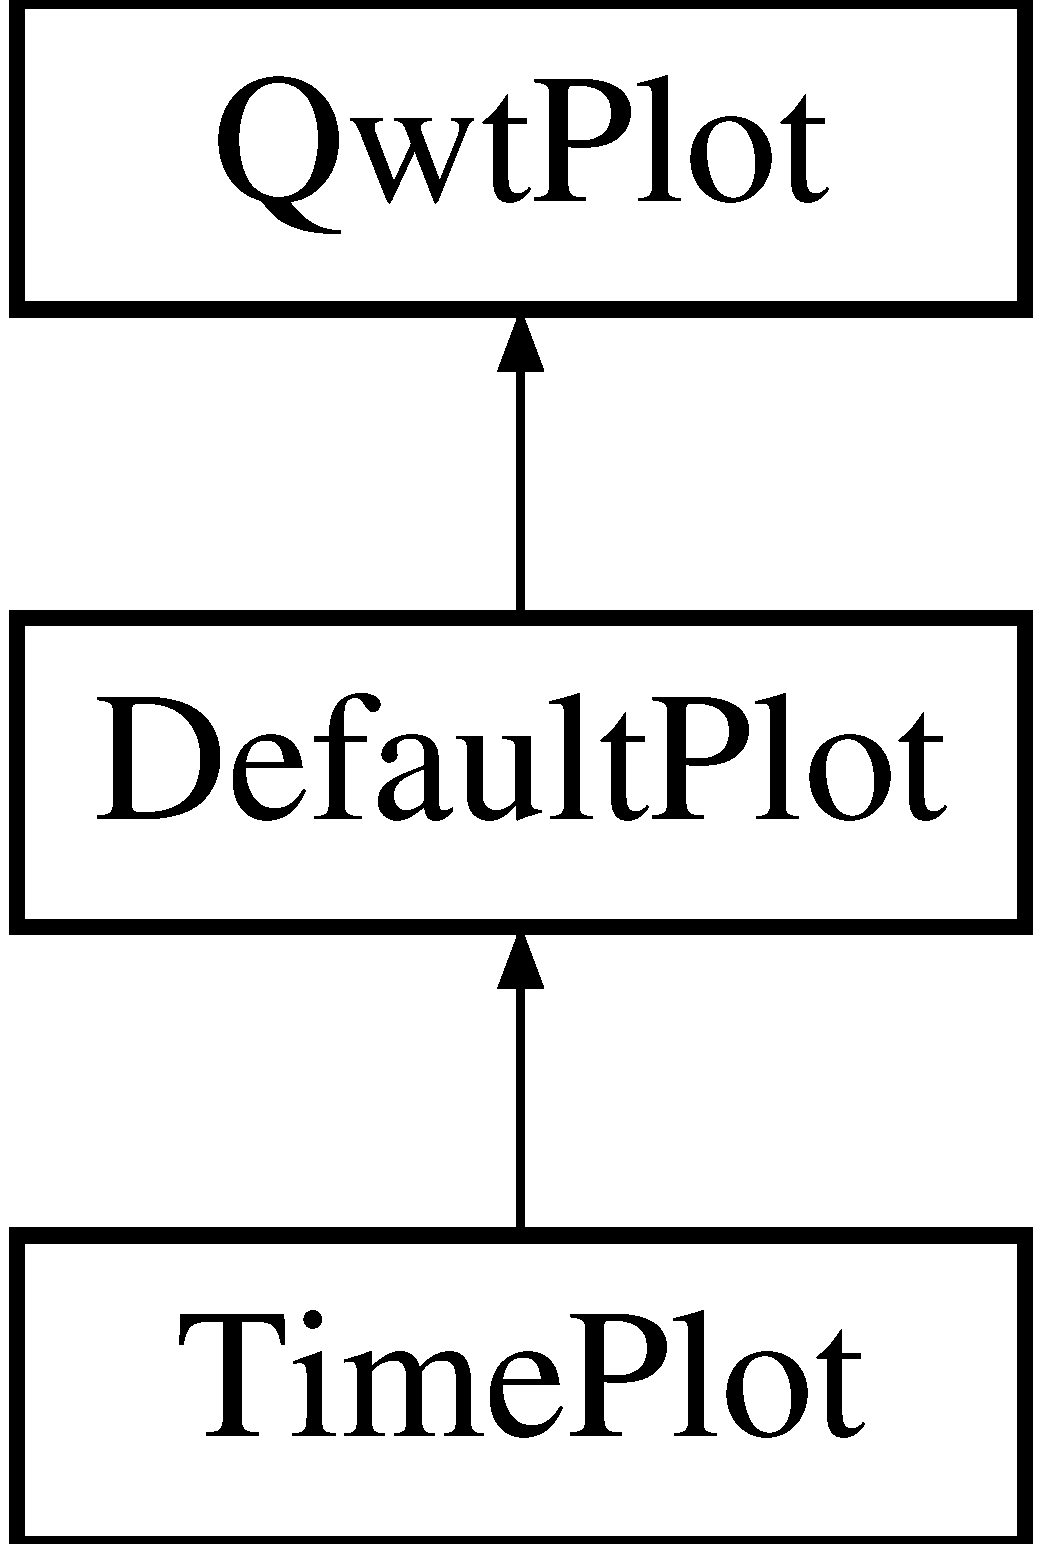
\includegraphics[height=3.000000cm]{class_time_plot}
\end{center}
\end{figure}
\subsection*{Public Slots}
\begin{DoxyCompactItemize}
\item 
void \hyperlink{class_time_plot_aaf0a9dc901fa6cca98ab9bc7ac0d8ab8}{add\+Value} (double value, int id\+\_\+electrode)
\item 
void \hyperlink{class_time_plot_a75ac3adcc3fa43c189e5c762e8536ffd}{add\+Value} (double value\+Time, double Value\+Potential, int id\+\_\+electrode)
\item 
void \hyperlink{class_time_plot_ad90e7c8e1e4a5bb9d342d55aaf02c61d}{add\+Value\+\_\+e1} (double value\+Time, double value)
\item 
void \hyperlink{class_time_plot_a5f86824066b46234e44c1181c273f01b}{add\+Value\+\_\+e2} (double value\+Time, double value)
\item 
void \hyperlink{class_time_plot_afe89c6014d11cde97e6a39e9ce33ad21}{add\+Value\+\_\+e3} (double value\+Time, double value)
\item 
void \hyperlink{class_time_plot_aa97d05708f827591712ee6fc487d6433}{pane\+Left} ()
\item 
void \hyperlink{class_time_plot_a0fcaf8e55c91bb77bc5fe277f479c4c4}{pane\+Right} ()
\item 
void \hyperlink{class_time_plot_ae21bba56d85e102c911acaa44627e0cc}{pane\+Up} ()
\item 
void \hyperlink{class_time_plot_a08ae17f53a7df7ad3bd3f2262bd83ebd}{pane\+Down} ()
\item 
void \hyperlink{class_time_plot_a60cb1a4789413379c9d520a329d766f0}{clear} ()
\item 
void \hyperlink{class_time_plot_a2d92b4dd295819801ae7f53d5c077242}{zoom\+In\+X} ()
\item 
void \hyperlink{class_time_plot_a2aecd88f70634747f6368c786578fbfe}{zoom\+Out\+X} ()
\item 
void \hyperlink{class_time_plot_aba49b973f5a79f81d70b7e0ea96a3206}{zoom\+In\+Y} ()
\item 
void \hyperlink{class_time_plot_ace67808742a97c6456689c2c1e30610f}{zoom\+Out\+Y} ()
\item 
void \hyperlink{class_time_plot_a830ae71cb3450da6aa98e6ae0344c54d}{autoscale} ()
\end{DoxyCompactItemize}
\subsection*{Public Member Functions}
\begin{DoxyCompactItemize}
\item 
\hyperlink{class_time_plot_a880ba93ed4a2fc6b29223517c4471f51}{Time\+Plot} (Q\+Widget $\ast$=N\+U\+L\+L)
\end{DoxyCompactItemize}
\subsection*{Additional Inherited Members}


\subsection{Constructor \& Destructor Documentation}
\hypertarget{class_time_plot_a880ba93ed4a2fc6b29223517c4471f51}{\index{Time\+Plot@{Time\+Plot}!Time\+Plot@{Time\+Plot}}
\index{Time\+Plot@{Time\+Plot}!Time\+Plot@{Time\+Plot}}
\subsubsection[{Time\+Plot}]{\setlength{\rightskip}{0pt plus 5cm}Time\+Plot\+::\+Time\+Plot (
\begin{DoxyParamCaption}
\item[{Q\+Widget $\ast$}]{parent = {\ttfamily NULL}}
\end{DoxyParamCaption}
)}}\label{class_time_plot_a880ba93ed4a2fc6b29223517c4471f51}


\subsection{Member Function Documentation}
\hypertarget{class_time_plot_aaf0a9dc901fa6cca98ab9bc7ac0d8ab8}{\index{Time\+Plot@{Time\+Plot}!add\+Value@{add\+Value}}
\index{add\+Value@{add\+Value}!Time\+Plot@{Time\+Plot}}
\subsubsection[{add\+Value}]{\setlength{\rightskip}{0pt plus 5cm}void Time\+Plot\+::add\+Value (
\begin{DoxyParamCaption}
\item[{double}]{value, }
\item[{int}]{id\+\_\+electrode}
\end{DoxyParamCaption}
)\hspace{0.3cm}{\ttfamily [slot]}}}\label{class_time_plot_aaf0a9dc901fa6cca98ab9bc7ac0d8ab8}
\hypertarget{class_time_plot_a75ac3adcc3fa43c189e5c762e8536ffd}{\index{Time\+Plot@{Time\+Plot}!add\+Value@{add\+Value}}
\index{add\+Value@{add\+Value}!Time\+Plot@{Time\+Plot}}
\subsubsection[{add\+Value}]{\setlength{\rightskip}{0pt plus 5cm}void Time\+Plot\+::add\+Value (
\begin{DoxyParamCaption}
\item[{double}]{value\+Time, }
\item[{double}]{Value\+Potential, }
\item[{int}]{id\+\_\+electrode}
\end{DoxyParamCaption}
)\hspace{0.3cm}{\ttfamily [slot]}}}\label{class_time_plot_a75ac3adcc3fa43c189e5c762e8536ffd}
\hypertarget{class_time_plot_ad90e7c8e1e4a5bb9d342d55aaf02c61d}{\index{Time\+Plot@{Time\+Plot}!add\+Value\+\_\+e1@{add\+Value\+\_\+e1}}
\index{add\+Value\+\_\+e1@{add\+Value\+\_\+e1}!Time\+Plot@{Time\+Plot}}
\subsubsection[{add\+Value\+\_\+e1}]{\setlength{\rightskip}{0pt plus 5cm}void Time\+Plot\+::add\+Value\+\_\+e1 (
\begin{DoxyParamCaption}
\item[{double}]{value\+Time, }
\item[{double}]{value}
\end{DoxyParamCaption}
)\hspace{0.3cm}{\ttfamily [slot]}}}\label{class_time_plot_ad90e7c8e1e4a5bb9d342d55aaf02c61d}
\hypertarget{class_time_plot_a5f86824066b46234e44c1181c273f01b}{\index{Time\+Plot@{Time\+Plot}!add\+Value\+\_\+e2@{add\+Value\+\_\+e2}}
\index{add\+Value\+\_\+e2@{add\+Value\+\_\+e2}!Time\+Plot@{Time\+Plot}}
\subsubsection[{add\+Value\+\_\+e2}]{\setlength{\rightskip}{0pt plus 5cm}void Time\+Plot\+::add\+Value\+\_\+e2 (
\begin{DoxyParamCaption}
\item[{double}]{value\+Time, }
\item[{double}]{value}
\end{DoxyParamCaption}
)\hspace{0.3cm}{\ttfamily [slot]}}}\label{class_time_plot_a5f86824066b46234e44c1181c273f01b}
\hypertarget{class_time_plot_afe89c6014d11cde97e6a39e9ce33ad21}{\index{Time\+Plot@{Time\+Plot}!add\+Value\+\_\+e3@{add\+Value\+\_\+e3}}
\index{add\+Value\+\_\+e3@{add\+Value\+\_\+e3}!Time\+Plot@{Time\+Plot}}
\subsubsection[{add\+Value\+\_\+e3}]{\setlength{\rightskip}{0pt plus 5cm}void Time\+Plot\+::add\+Value\+\_\+e3 (
\begin{DoxyParamCaption}
\item[{double}]{value\+Time, }
\item[{double}]{value}
\end{DoxyParamCaption}
)\hspace{0.3cm}{\ttfamily [slot]}}}\label{class_time_plot_afe89c6014d11cde97e6a39e9ce33ad21}
\hypertarget{class_time_plot_a830ae71cb3450da6aa98e6ae0344c54d}{\index{Time\+Plot@{Time\+Plot}!autoscale@{autoscale}}
\index{autoscale@{autoscale}!Time\+Plot@{Time\+Plot}}
\subsubsection[{autoscale}]{\setlength{\rightskip}{0pt plus 5cm}void Time\+Plot\+::autoscale (
\begin{DoxyParamCaption}
{}
\end{DoxyParamCaption}
)\hspace{0.3cm}{\ttfamily [slot]}}}\label{class_time_plot_a830ae71cb3450da6aa98e6ae0344c54d}
\hypertarget{class_time_plot_a60cb1a4789413379c9d520a329d766f0}{\index{Time\+Plot@{Time\+Plot}!clear@{clear}}
\index{clear@{clear}!Time\+Plot@{Time\+Plot}}
\subsubsection[{clear}]{\setlength{\rightskip}{0pt plus 5cm}void Time\+Plot\+::clear (
\begin{DoxyParamCaption}
{}
\end{DoxyParamCaption}
)\hspace{0.3cm}{\ttfamily [slot]}}}\label{class_time_plot_a60cb1a4789413379c9d520a329d766f0}
\hypertarget{class_time_plot_a08ae17f53a7df7ad3bd3f2262bd83ebd}{\index{Time\+Plot@{Time\+Plot}!pane\+Down@{pane\+Down}}
\index{pane\+Down@{pane\+Down}!Time\+Plot@{Time\+Plot}}
\subsubsection[{pane\+Down}]{\setlength{\rightskip}{0pt plus 5cm}void Time\+Plot\+::pane\+Down (
\begin{DoxyParamCaption}
{}
\end{DoxyParamCaption}
)\hspace{0.3cm}{\ttfamily [slot]}}}\label{class_time_plot_a08ae17f53a7df7ad3bd3f2262bd83ebd}
\hypertarget{class_time_plot_aa97d05708f827591712ee6fc487d6433}{\index{Time\+Plot@{Time\+Plot}!pane\+Left@{pane\+Left}}
\index{pane\+Left@{pane\+Left}!Time\+Plot@{Time\+Plot}}
\subsubsection[{pane\+Left}]{\setlength{\rightskip}{0pt plus 5cm}void Time\+Plot\+::pane\+Left (
\begin{DoxyParamCaption}
{}
\end{DoxyParamCaption}
)\hspace{0.3cm}{\ttfamily [slot]}}}\label{class_time_plot_aa97d05708f827591712ee6fc487d6433}
\hypertarget{class_time_plot_a0fcaf8e55c91bb77bc5fe277f479c4c4}{\index{Time\+Plot@{Time\+Plot}!pane\+Right@{pane\+Right}}
\index{pane\+Right@{pane\+Right}!Time\+Plot@{Time\+Plot}}
\subsubsection[{pane\+Right}]{\setlength{\rightskip}{0pt plus 5cm}void Time\+Plot\+::pane\+Right (
\begin{DoxyParamCaption}
{}
\end{DoxyParamCaption}
)\hspace{0.3cm}{\ttfamily [slot]}}}\label{class_time_plot_a0fcaf8e55c91bb77bc5fe277f479c4c4}
\hypertarget{class_time_plot_ae21bba56d85e102c911acaa44627e0cc}{\index{Time\+Plot@{Time\+Plot}!pane\+Up@{pane\+Up}}
\index{pane\+Up@{pane\+Up}!Time\+Plot@{Time\+Plot}}
\subsubsection[{pane\+Up}]{\setlength{\rightskip}{0pt plus 5cm}void Time\+Plot\+::pane\+Up (
\begin{DoxyParamCaption}
{}
\end{DoxyParamCaption}
)\hspace{0.3cm}{\ttfamily [slot]}}}\label{class_time_plot_ae21bba56d85e102c911acaa44627e0cc}
\hypertarget{class_time_plot_a2d92b4dd295819801ae7f53d5c077242}{\index{Time\+Plot@{Time\+Plot}!zoom\+In\+X@{zoom\+In\+X}}
\index{zoom\+In\+X@{zoom\+In\+X}!Time\+Plot@{Time\+Plot}}
\subsubsection[{zoom\+In\+X}]{\setlength{\rightskip}{0pt plus 5cm}void Time\+Plot\+::zoom\+In\+X (
\begin{DoxyParamCaption}
{}
\end{DoxyParamCaption}
)\hspace{0.3cm}{\ttfamily [slot]}}}\label{class_time_plot_a2d92b4dd295819801ae7f53d5c077242}
\hypertarget{class_time_plot_aba49b973f5a79f81d70b7e0ea96a3206}{\index{Time\+Plot@{Time\+Plot}!zoom\+In\+Y@{zoom\+In\+Y}}
\index{zoom\+In\+Y@{zoom\+In\+Y}!Time\+Plot@{Time\+Plot}}
\subsubsection[{zoom\+In\+Y}]{\setlength{\rightskip}{0pt plus 5cm}void Time\+Plot\+::zoom\+In\+Y (
\begin{DoxyParamCaption}
{}
\end{DoxyParamCaption}
)\hspace{0.3cm}{\ttfamily [slot]}}}\label{class_time_plot_aba49b973f5a79f81d70b7e0ea96a3206}
\hypertarget{class_time_plot_a2aecd88f70634747f6368c786578fbfe}{\index{Time\+Plot@{Time\+Plot}!zoom\+Out\+X@{zoom\+Out\+X}}
\index{zoom\+Out\+X@{zoom\+Out\+X}!Time\+Plot@{Time\+Plot}}
\subsubsection[{zoom\+Out\+X}]{\setlength{\rightskip}{0pt plus 5cm}void Time\+Plot\+::zoom\+Out\+X (
\begin{DoxyParamCaption}
{}
\end{DoxyParamCaption}
)\hspace{0.3cm}{\ttfamily [slot]}}}\label{class_time_plot_a2aecd88f70634747f6368c786578fbfe}
\hypertarget{class_time_plot_ace67808742a97c6456689c2c1e30610f}{\index{Time\+Plot@{Time\+Plot}!zoom\+Out\+Y@{zoom\+Out\+Y}}
\index{zoom\+Out\+Y@{zoom\+Out\+Y}!Time\+Plot@{Time\+Plot}}
\subsubsection[{zoom\+Out\+Y}]{\setlength{\rightskip}{0pt plus 5cm}void Time\+Plot\+::zoom\+Out\+Y (
\begin{DoxyParamCaption}
{}
\end{DoxyParamCaption}
)\hspace{0.3cm}{\ttfamily [slot]}}}\label{class_time_plot_ace67808742a97c6456689c2c1e30610f}


The documentation for this class was generated from the following files\+:\begin{DoxyCompactItemize}
\item 
\hyperlink{time_plot_8h}{time\+Plot.\+h}\item 
\hyperlink{time_plot_8cpp}{time\+Plot.\+cpp}\end{DoxyCompactItemize}

\hypertarget{struct_timestep_node}{\section{Timestep\+Node Struct Reference}
\label{struct_timestep_node}\index{Timestep\+Node@{Timestep\+Node}}
}


{\ttfamily \#include $<$Timestep\+Node.\+h$>$}

\subsection*{Public Attributes}
\begin{DoxyCompactItemize}
\item 
double \hyperlink{struct_timestep_node_a596f2f628083ecba5bd61055927e3c1e}{timestep}
\item 
\hyperlink{class_oscillator}{Oscillator} $\ast$ \hyperlink{struct_timestep_node_a7db200fe304dd9587bf2f3e361b49b5b}{osc}
\end{DoxyCompactItemize}


\subsection{Member Data Documentation}
\hypertarget{struct_timestep_node_a7db200fe304dd9587bf2f3e361b49b5b}{\index{Timestep\+Node@{Timestep\+Node}!osc@{osc}}
\index{osc@{osc}!Timestep\+Node@{Timestep\+Node}}
\subsubsection[{osc}]{\setlength{\rightskip}{0pt plus 5cm}{\bf Oscillator}$\ast$ Timestep\+Node\+::osc}}\label{struct_timestep_node_a7db200fe304dd9587bf2f3e361b49b5b}
\hypertarget{struct_timestep_node_a596f2f628083ecba5bd61055927e3c1e}{\index{Timestep\+Node@{Timestep\+Node}!timestep@{timestep}}
\index{timestep@{timestep}!Timestep\+Node@{Timestep\+Node}}
\subsubsection[{timestep}]{\setlength{\rightskip}{0pt plus 5cm}double Timestep\+Node\+::timestep}}\label{struct_timestep_node_a596f2f628083ecba5bd61055927e3c1e}


The documentation for this struct was generated from the following file\+:\begin{DoxyCompactItemize}
\item 
Numeric\+Strategy/\hyperlink{_timestep_node_8h}{Timestep\+Node.\+h}\end{DoxyCompactItemize}

\hypertarget{struct_time_tree}{\section{Time\+Tree Struct Reference}
\label{struct_time_tree}\index{Time\+Tree@{Time\+Tree}}
}


{\ttfamily \#include $<$Time\+Tree.\+h$>$}

\subsection*{Public Attributes}
\begin{DoxyCompactItemize}
\item 
double \hyperlink{struct_time_tree_a37fb85a78a8d379e61ffb910c0028597}{time}
\item 
\hyperlink{struct_time_tree}{Time\+Tree} $\ast$ \hyperlink{struct_time_tree_a46ade43f75331b3d9582a3f0da6431c9}{earlier\+Node}
\item 
\hyperlink{struct_time_tree}{Time\+Tree} $\ast$ \hyperlink{struct_time_tree_aabf289bfd36c7bacba47caf3e54d9e85}{later\+Node}
\item 
\hyperlink{struct_time_tree}{Time\+Tree} $\ast$ \hyperlink{struct_time_tree_a48e012db090e102c3970b3bf1d77ea3a}{parent\+Node}
\item 
\hyperlink{class_oscillator}{Oscillator} $\ast$ \hyperlink{struct_time_tree_a4facb804fe4af183557b396ce218aacc}{osc}
\end{DoxyCompactItemize}


\subsection{Member Data Documentation}
\hypertarget{struct_time_tree_a46ade43f75331b3d9582a3f0da6431c9}{\index{Time\+Tree@{Time\+Tree}!earlier\+Node@{earlier\+Node}}
\index{earlier\+Node@{earlier\+Node}!Time\+Tree@{Time\+Tree}}
\subsubsection[{earlier\+Node}]{\setlength{\rightskip}{0pt plus 5cm}{\bf Time\+Tree}$\ast$ Time\+Tree\+::earlier\+Node}}\label{struct_time_tree_a46ade43f75331b3d9582a3f0da6431c9}
\hypertarget{struct_time_tree_aabf289bfd36c7bacba47caf3e54d9e85}{\index{Time\+Tree@{Time\+Tree}!later\+Node@{later\+Node}}
\index{later\+Node@{later\+Node}!Time\+Tree@{Time\+Tree}}
\subsubsection[{later\+Node}]{\setlength{\rightskip}{0pt plus 5cm}{\bf Time\+Tree}$\ast$ Time\+Tree\+::later\+Node}}\label{struct_time_tree_aabf289bfd36c7bacba47caf3e54d9e85}
\hypertarget{struct_time_tree_a4facb804fe4af183557b396ce218aacc}{\index{Time\+Tree@{Time\+Tree}!osc@{osc}}
\index{osc@{osc}!Time\+Tree@{Time\+Tree}}
\subsubsection[{osc}]{\setlength{\rightskip}{0pt plus 5cm}{\bf Oscillator}$\ast$ Time\+Tree\+::osc}}\label{struct_time_tree_a4facb804fe4af183557b396ce218aacc}
\hypertarget{struct_time_tree_a48e012db090e102c3970b3bf1d77ea3a}{\index{Time\+Tree@{Time\+Tree}!parent\+Node@{parent\+Node}}
\index{parent\+Node@{parent\+Node}!Time\+Tree@{Time\+Tree}}
\subsubsection[{parent\+Node}]{\setlength{\rightskip}{0pt plus 5cm}{\bf Time\+Tree}$\ast$ Time\+Tree\+::parent\+Node}}\label{struct_time_tree_a48e012db090e102c3970b3bf1d77ea3a}
\hypertarget{struct_time_tree_a37fb85a78a8d379e61ffb910c0028597}{\index{Time\+Tree@{Time\+Tree}!time@{time}}
\index{time@{time}!Time\+Tree@{Time\+Tree}}
\subsubsection[{time}]{\setlength{\rightskip}{0pt plus 5cm}double Time\+Tree\+::time}}\label{struct_time_tree_a37fb85a78a8d379e61ffb910c0028597}


The documentation for this struct was generated from the following file\+:\begin{DoxyCompactItemize}
\item 
Numeric\+Strategy/\hyperlink{_time_tree_8h}{Time\+Tree.\+h}\end{DoxyCompactItemize}

\hypertarget{structt_vector3}{\section{t\+Vector3 Struct Reference}
\label{structt_vector3}\index{t\+Vector3@{t\+Vector3}}
}


{\ttfamily \#include $<$G\+Lcamera.\+h$>$}

\subsection*{Public Member Functions}
\begin{DoxyCompactItemize}
\item 
\hyperlink{structt_vector3_a2d8c2e565268f2b90fc9bc60e6f89a35}{t\+Vector3} ()
\item 
\hyperlink{structt_vector3_ada2c2fab7bb7152b95be6e7c1a16be4c}{t\+Vector3} (float new\+\_\+x, float new\+\_\+y, float new\+\_\+z)
\item 
\hyperlink{structt_vector3}{t\+Vector3} \hyperlink{structt_vector3_a30a2afe00fea19f80180750988e758cf}{operator+} (\hyperlink{structt_vector3}{t\+Vector3} v\+Vector)
\item 
\hyperlink{structt_vector3}{t\+Vector3} \hyperlink{structt_vector3_a620e3f05ae5b72e1ca51ab8f5e79f2d9}{operator-\/} (\hyperlink{structt_vector3}{t\+Vector3} v\+Vector)
\item 
\hyperlink{structt_vector3}{t\+Vector3} \hyperlink{structt_vector3_ad00a82939bd0fa68ff90e378ff6592ee}{operator$\ast$} (float number)
\item 
\hyperlink{structt_vector3}{t\+Vector3} \hyperlink{structt_vector3_a0e7f54e0c885a9e994b04e4ee21959d2}{operator$^\wedge$} (\hyperlink{structt_vector3}{t\+Vector3} v\+Vector)
\item 
\hyperlink{structt_vector3}{t\+Vector3} \hyperlink{structt_vector3_a87476053d638c3e648570f2e02c1cc1d}{operator/} (float number)
\end{DoxyCompactItemize}
\subsection*{Public Attributes}
\begin{DoxyCompactItemize}
\item 
float \hyperlink{structt_vector3_a424ec48e8f7aab656bafa5796f493385}{x}
\item 
float \hyperlink{structt_vector3_ab2c9e6ddeb1bf79a3e85b264549efb3b}{y}
\item 
float \hyperlink{structt_vector3_abdbd8e973fd4634920a44119f329920f}{z}
\end{DoxyCompactItemize}


\subsection{Constructor \& Destructor Documentation}
\hypertarget{structt_vector3_a2d8c2e565268f2b90fc9bc60e6f89a35}{\index{t\+Vector3@{t\+Vector3}!t\+Vector3@{t\+Vector3}}
\index{t\+Vector3@{t\+Vector3}!t\+Vector3@{t\+Vector3}}
\subsubsection[{t\+Vector3}]{\setlength{\rightskip}{0pt plus 5cm}t\+Vector3\+::t\+Vector3 (
\begin{DoxyParamCaption}
{}
\end{DoxyParamCaption}
)\hspace{0.3cm}{\ttfamily [inline]}}}\label{structt_vector3_a2d8c2e565268f2b90fc9bc60e6f89a35}
\hypertarget{structt_vector3_ada2c2fab7bb7152b95be6e7c1a16be4c}{\index{t\+Vector3@{t\+Vector3}!t\+Vector3@{t\+Vector3}}
\index{t\+Vector3@{t\+Vector3}!t\+Vector3@{t\+Vector3}}
\subsubsection[{t\+Vector3}]{\setlength{\rightskip}{0pt plus 5cm}t\+Vector3\+::t\+Vector3 (
\begin{DoxyParamCaption}
\item[{float}]{new\+\_\+x, }
\item[{float}]{new\+\_\+y, }
\item[{float}]{new\+\_\+z}
\end{DoxyParamCaption}
)\hspace{0.3cm}{\ttfamily [inline]}}}\label{structt_vector3_ada2c2fab7bb7152b95be6e7c1a16be4c}


\subsection{Member Function Documentation}
\hypertarget{structt_vector3_ad00a82939bd0fa68ff90e378ff6592ee}{\index{t\+Vector3@{t\+Vector3}!operator$\ast$@{operator$\ast$}}
\index{operator$\ast$@{operator$\ast$}!t\+Vector3@{t\+Vector3}}
\subsubsection[{operator$\ast$}]{\setlength{\rightskip}{0pt plus 5cm}{\bf t\+Vector3} t\+Vector3\+::operator$\ast$ (
\begin{DoxyParamCaption}
\item[{float}]{number}
\end{DoxyParamCaption}
)\hspace{0.3cm}{\ttfamily [inline]}}}\label{structt_vector3_ad00a82939bd0fa68ff90e378ff6592ee}
\hypertarget{structt_vector3_a30a2afe00fea19f80180750988e758cf}{\index{t\+Vector3@{t\+Vector3}!operator+@{operator+}}
\index{operator+@{operator+}!t\+Vector3@{t\+Vector3}}
\subsubsection[{operator+}]{\setlength{\rightskip}{0pt plus 5cm}{\bf t\+Vector3} t\+Vector3\+::operator+ (
\begin{DoxyParamCaption}
\item[{{\bf t\+Vector3}}]{v\+Vector}
\end{DoxyParamCaption}
)\hspace{0.3cm}{\ttfamily [inline]}}}\label{structt_vector3_a30a2afe00fea19f80180750988e758cf}
\hypertarget{structt_vector3_a620e3f05ae5b72e1ca51ab8f5e79f2d9}{\index{t\+Vector3@{t\+Vector3}!operator-\/@{operator-\/}}
\index{operator-\/@{operator-\/}!t\+Vector3@{t\+Vector3}}
\subsubsection[{operator-\/}]{\setlength{\rightskip}{0pt plus 5cm}{\bf t\+Vector3} t\+Vector3\+::operator-\/ (
\begin{DoxyParamCaption}
\item[{{\bf t\+Vector3}}]{v\+Vector}
\end{DoxyParamCaption}
)\hspace{0.3cm}{\ttfamily [inline]}}}\label{structt_vector3_a620e3f05ae5b72e1ca51ab8f5e79f2d9}
\hypertarget{structt_vector3_a87476053d638c3e648570f2e02c1cc1d}{\index{t\+Vector3@{t\+Vector3}!operator/@{operator/}}
\index{operator/@{operator/}!t\+Vector3@{t\+Vector3}}
\subsubsection[{operator/}]{\setlength{\rightskip}{0pt plus 5cm}{\bf t\+Vector3} t\+Vector3\+::operator/ (
\begin{DoxyParamCaption}
\item[{float}]{number}
\end{DoxyParamCaption}
)\hspace{0.3cm}{\ttfamily [inline]}}}\label{structt_vector3_a87476053d638c3e648570f2e02c1cc1d}
\hypertarget{structt_vector3_a0e7f54e0c885a9e994b04e4ee21959d2}{\index{t\+Vector3@{t\+Vector3}!operator$^\wedge$@{operator$^\wedge$}}
\index{operator$^\wedge$@{operator$^\wedge$}!t\+Vector3@{t\+Vector3}}
\subsubsection[{operator$^\wedge$}]{\setlength{\rightskip}{0pt plus 5cm}{\bf t\+Vector3} t\+Vector3\+::operator$^\wedge$ (
\begin{DoxyParamCaption}
\item[{{\bf t\+Vector3}}]{v\+Vector}
\end{DoxyParamCaption}
)\hspace{0.3cm}{\ttfamily [inline]}}}\label{structt_vector3_a0e7f54e0c885a9e994b04e4ee21959d2}


\subsection{Member Data Documentation}
\hypertarget{structt_vector3_a424ec48e8f7aab656bafa5796f493385}{\index{t\+Vector3@{t\+Vector3}!x@{x}}
\index{x@{x}!t\+Vector3@{t\+Vector3}}
\subsubsection[{x}]{\setlength{\rightskip}{0pt plus 5cm}float t\+Vector3\+::x}}\label{structt_vector3_a424ec48e8f7aab656bafa5796f493385}
\hypertarget{structt_vector3_ab2c9e6ddeb1bf79a3e85b264549efb3b}{\index{t\+Vector3@{t\+Vector3}!y@{y}}
\index{y@{y}!t\+Vector3@{t\+Vector3}}
\subsubsection[{y}]{\setlength{\rightskip}{0pt plus 5cm}float t\+Vector3\+::y}}\label{structt_vector3_ab2c9e6ddeb1bf79a3e85b264549efb3b}
\hypertarget{structt_vector3_abdbd8e973fd4634920a44119f329920f}{\index{t\+Vector3@{t\+Vector3}!z@{z}}
\index{z@{z}!t\+Vector3@{t\+Vector3}}
\subsubsection[{z}]{\setlength{\rightskip}{0pt plus 5cm}float t\+Vector3\+::z}}\label{structt_vector3_abdbd8e973fd4634920a44119f329920f}


The documentation for this struct was generated from the following file\+:\begin{DoxyCompactItemize}
\item 
\hyperlink{_g_lcamera_8h}{G\+Lcamera.\+h}\end{DoxyCompactItemize}

\hypertarget{classv3model}{\section{v3model Class Reference}
\label{classv3model}\index{v3model@{v3model}}
}


{\ttfamily \#include $<$v3model.\+h$>$}

Inheritance diagram for v3model\+:\begin{figure}[H]
\begin{center}
\leavevmode
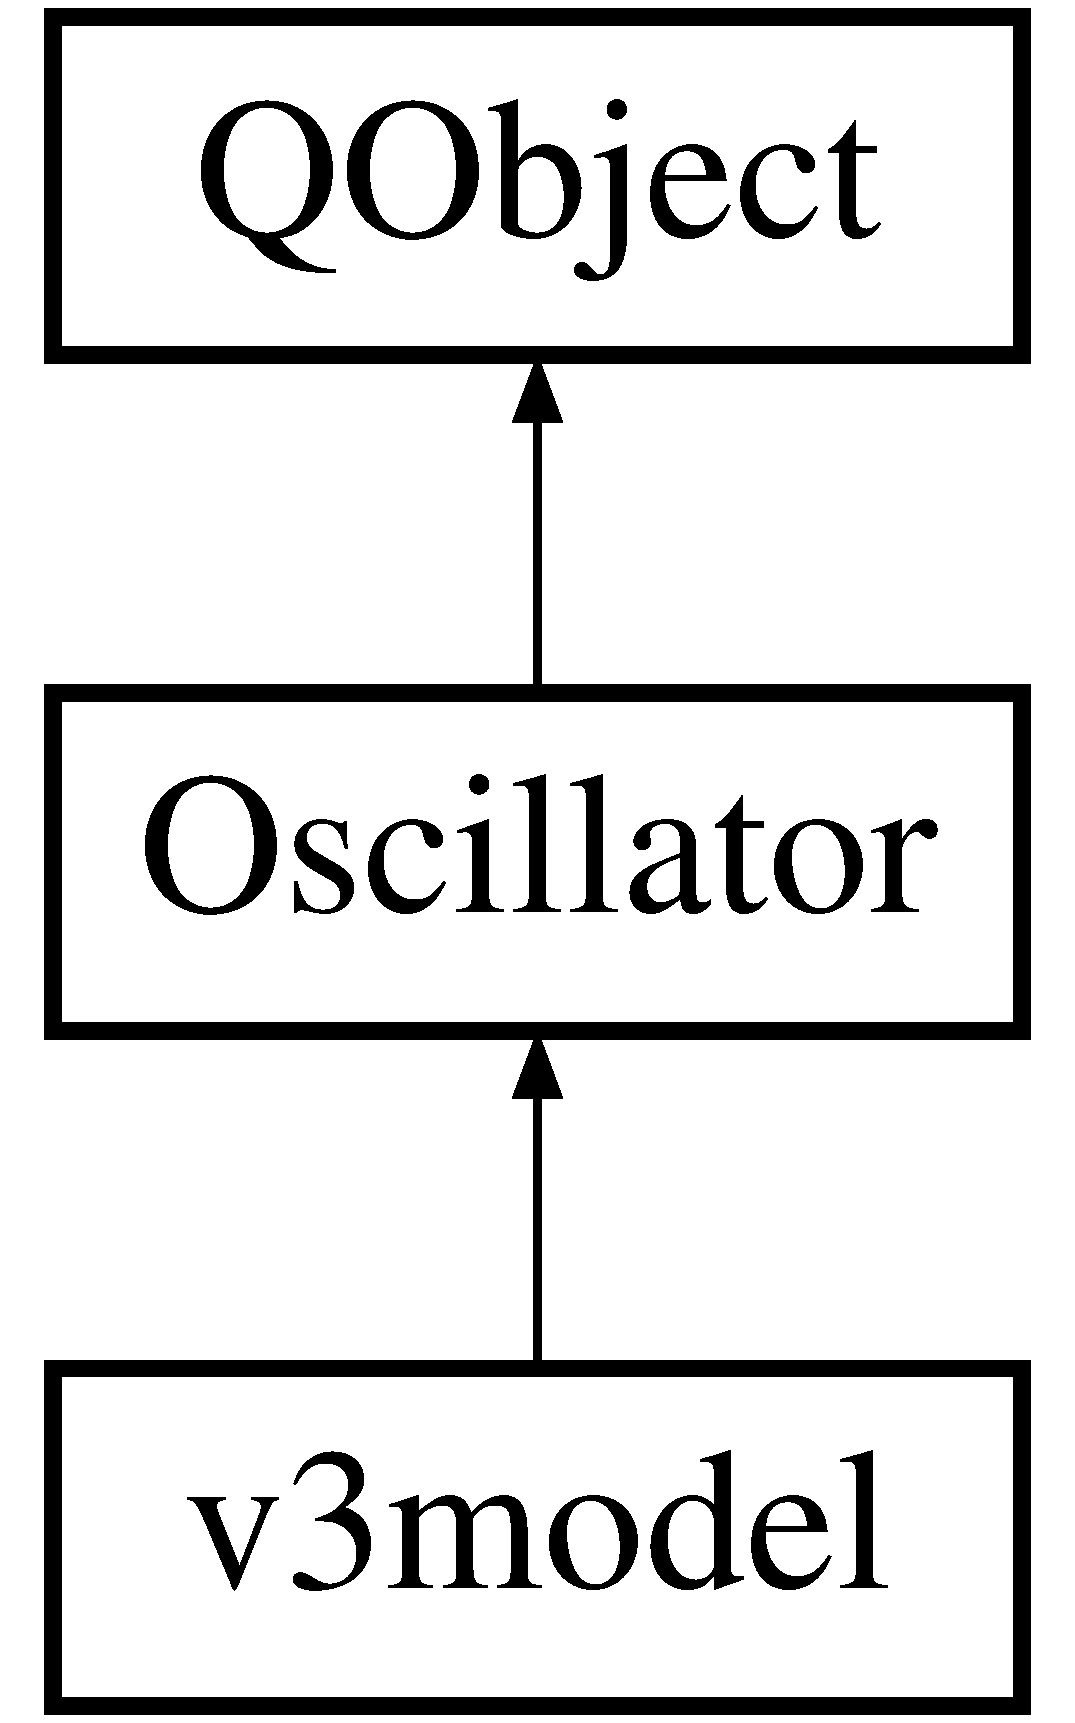
\includegraphics[height=3.000000cm]{classv3model}
\end{center}
\end{figure}
\subsection*{Public Slots}
\begin{DoxyCompactItemize}
\item 
void \hyperlink{classv3model_a1ce58dd6384772b84a7a3c3f73a70c3f}{set\+Parameter} (double value, \hyperlink{heart_defines_8h_a79395aba577c2bc57e7ca211ff3476a6}{O\+S\+C\+\_\+\+P\+A\+R\+A\+M\+E\+T\+E\+R} parameter)
\item 
void \hyperlink{classv3model_a7b930af4a46f46aaa3301947526c556d}{set\+E\+R\+P} (double value)
\end{DoxyCompactItemize}
\subsection*{Public Member Functions}
\begin{DoxyCompactItemize}
\item 
\hyperlink{classv3model_aa3c5a02561c2a8e14f80b599f35c8be3}{v3model} (void)
\item 
\hyperlink{classv3model_a78cbf845aa6ab504372a8710cad28f4b}{$\sim$v3model} (void)
\item 
double \hyperlink{classv3model_a14957985c821508b7a5985a423d0c942}{get\+Current\+Prim} (const int \&which)
\item 
double \hyperlink{classv3model_a7db295a02c2487b6eb4d13e6e942a088}{get\+Potential\+Prim} ()
\item 
double \hyperlink{classv3model_aeb8db7e7f6327e341b73ce6ee22c888a}{get\+E\+R\+P} ()
\item 
double \hyperlink{classv3model_a18cfce2a9bc0536157da81cef399706a}{get\+\_\+p} ()
\begin{DoxyCompactList}\small\item\em virtual function for refractory period setting \end{DoxyCompactList}\item 
double \hyperlink{classv3model_ad969fd48215103f85ce383f11d759c99}{get\+\_\+q} ()
\item 
double \hyperlink{classv3model_a78dfba3662698b7967b683b975f473bb}{get\+\_\+tau\+\_\+d} ()
\item 
double \hyperlink{classv3model_a697f47117c9921dcb0e6da322a41ed1a}{get\+\_\+\+J\+\_\+fi} ()
\item 
double \hyperlink{classv3model_a1eb045a08d91e3677e25c298044046df}{get\+\_\+tau\+\_\+v\+\_\+minus} ()
\item 
double \hyperlink{classv3model_a0e4cf672a486a8334967c880606925a9}{get\+\_\+\+J\+\_\+so} ()
\item 
double \hyperlink{classv3model_ac852daced9f1246ce321d8245320b345}{get\+\_\+\+J\+\_\+si} ()
\end{DoxyCompactItemize}
\subsection*{Additional Inherited Members}


\subsection{Constructor \& Destructor Documentation}
\hypertarget{classv3model_aa3c5a02561c2a8e14f80b599f35c8be3}{\index{v3model@{v3model}!v3model@{v3model}}
\index{v3model@{v3model}!v3model@{v3model}}
\subsubsection[{v3model}]{\setlength{\rightskip}{0pt plus 5cm}v3model\+::v3model (
\begin{DoxyParamCaption}
\item[{void}]{}
\end{DoxyParamCaption}
)}}\label{classv3model_aa3c5a02561c2a8e14f80b599f35c8be3}
\hypertarget{classv3model_a78cbf845aa6ab504372a8710cad28f4b}{\index{v3model@{v3model}!````~v3model@{$\sim$v3model}}
\index{````~v3model@{$\sim$v3model}!v3model@{v3model}}
\subsubsection[{$\sim$v3model}]{\setlength{\rightskip}{0pt plus 5cm}v3model\+::$\sim$v3model (
\begin{DoxyParamCaption}
\item[{void}]{}
\end{DoxyParamCaption}
)}}\label{classv3model_a78cbf845aa6ab504372a8710cad28f4b}


\subsection{Member Function Documentation}
\hypertarget{classv3model_a697f47117c9921dcb0e6da322a41ed1a}{\index{v3model@{v3model}!get\+\_\+\+J\+\_\+fi@{get\+\_\+\+J\+\_\+fi}}
\index{get\+\_\+\+J\+\_\+fi@{get\+\_\+\+J\+\_\+fi}!v3model@{v3model}}
\subsubsection[{get\+\_\+\+J\+\_\+fi}]{\setlength{\rightskip}{0pt plus 5cm}double v3model\+::get\+\_\+\+J\+\_\+fi (
\begin{DoxyParamCaption}
{}
\end{DoxyParamCaption}
)}}\label{classv3model_a697f47117c9921dcb0e6da322a41ed1a}
\hypertarget{classv3model_ac852daced9f1246ce321d8245320b345}{\index{v3model@{v3model}!get\+\_\+\+J\+\_\+si@{get\+\_\+\+J\+\_\+si}}
\index{get\+\_\+\+J\+\_\+si@{get\+\_\+\+J\+\_\+si}!v3model@{v3model}}
\subsubsection[{get\+\_\+\+J\+\_\+si}]{\setlength{\rightskip}{0pt plus 5cm}double v3model\+::get\+\_\+\+J\+\_\+si (
\begin{DoxyParamCaption}
{}
\end{DoxyParamCaption}
)}}\label{classv3model_ac852daced9f1246ce321d8245320b345}
\hypertarget{classv3model_a0e4cf672a486a8334967c880606925a9}{\index{v3model@{v3model}!get\+\_\+\+J\+\_\+so@{get\+\_\+\+J\+\_\+so}}
\index{get\+\_\+\+J\+\_\+so@{get\+\_\+\+J\+\_\+so}!v3model@{v3model}}
\subsubsection[{get\+\_\+\+J\+\_\+so}]{\setlength{\rightskip}{0pt plus 5cm}double v3model\+::get\+\_\+\+J\+\_\+so (
\begin{DoxyParamCaption}
{}
\end{DoxyParamCaption}
)}}\label{classv3model_a0e4cf672a486a8334967c880606925a9}
\hypertarget{classv3model_a18cfce2a9bc0536157da81cef399706a}{\index{v3model@{v3model}!get\+\_\+p@{get\+\_\+p}}
\index{get\+\_\+p@{get\+\_\+p}!v3model@{v3model}}
\subsubsection[{get\+\_\+p}]{\setlength{\rightskip}{0pt plus 5cm}double v3model\+::get\+\_\+p (
\begin{DoxyParamCaption}
{}
\end{DoxyParamCaption}
)}}\label{classv3model_a18cfce2a9bc0536157da81cef399706a}


virtual function for refractory period setting 

\hypertarget{classv3model_ad969fd48215103f85ce383f11d759c99}{\index{v3model@{v3model}!get\+\_\+q@{get\+\_\+q}}
\index{get\+\_\+q@{get\+\_\+q}!v3model@{v3model}}
\subsubsection[{get\+\_\+q}]{\setlength{\rightskip}{0pt plus 5cm}double v3model\+::get\+\_\+q (
\begin{DoxyParamCaption}
{}
\end{DoxyParamCaption}
)}}\label{classv3model_ad969fd48215103f85ce383f11d759c99}
\hypertarget{classv3model_a78dfba3662698b7967b683b975f473bb}{\index{v3model@{v3model}!get\+\_\+tau\+\_\+d@{get\+\_\+tau\+\_\+d}}
\index{get\+\_\+tau\+\_\+d@{get\+\_\+tau\+\_\+d}!v3model@{v3model}}
\subsubsection[{get\+\_\+tau\+\_\+d}]{\setlength{\rightskip}{0pt plus 5cm}double v3model\+::get\+\_\+tau\+\_\+d (
\begin{DoxyParamCaption}
{}
\end{DoxyParamCaption}
)}}\label{classv3model_a78dfba3662698b7967b683b975f473bb}
\hypertarget{classv3model_a1eb045a08d91e3677e25c298044046df}{\index{v3model@{v3model}!get\+\_\+tau\+\_\+v\+\_\+minus@{get\+\_\+tau\+\_\+v\+\_\+minus}}
\index{get\+\_\+tau\+\_\+v\+\_\+minus@{get\+\_\+tau\+\_\+v\+\_\+minus}!v3model@{v3model}}
\subsubsection[{get\+\_\+tau\+\_\+v\+\_\+minus}]{\setlength{\rightskip}{0pt plus 5cm}double v3model\+::get\+\_\+tau\+\_\+v\+\_\+minus (
\begin{DoxyParamCaption}
{}
\end{DoxyParamCaption}
)}}\label{classv3model_a1eb045a08d91e3677e25c298044046df}
\hypertarget{classv3model_a14957985c821508b7a5985a423d0c942}{\index{v3model@{v3model}!get\+Current\+Prim@{get\+Current\+Prim}}
\index{get\+Current\+Prim@{get\+Current\+Prim}!v3model@{v3model}}
\subsubsection[{get\+Current\+Prim}]{\setlength{\rightskip}{0pt plus 5cm}double v3model\+::get\+Current\+Prim (
\begin{DoxyParamCaption}
\item[{const int \&}]{which}
\end{DoxyParamCaption}
)\hspace{0.3cm}{\ttfamily [virtual]}}}\label{classv3model_a14957985c821508b7a5985a423d0c942}


Reimplemented from \hyperlink{class_oscillator_a6132c7be8737a5686d64629b68b81743}{Oscillator}.

\hypertarget{classv3model_aeb8db7e7f6327e341b73ce6ee22c888a}{\index{v3model@{v3model}!get\+E\+R\+P@{get\+E\+R\+P}}
\index{get\+E\+R\+P@{get\+E\+R\+P}!v3model@{v3model}}
\subsubsection[{get\+E\+R\+P}]{\setlength{\rightskip}{0pt plus 5cm}double v3model\+::get\+E\+R\+P (
\begin{DoxyParamCaption}
{}
\end{DoxyParamCaption}
)\hspace{0.3cm}{\ttfamily [virtual]}}}\label{classv3model_aeb8db7e7f6327e341b73ce6ee22c888a}


Reimplemented from \hyperlink{class_oscillator_ae81ca9a4404d59af1eaea0526cc3c88e}{Oscillator}.

\hypertarget{classv3model_a7db295a02c2487b6eb4d13e6e942a088}{\index{v3model@{v3model}!get\+Potential\+Prim@{get\+Potential\+Prim}}
\index{get\+Potential\+Prim@{get\+Potential\+Prim}!v3model@{v3model}}
\subsubsection[{get\+Potential\+Prim}]{\setlength{\rightskip}{0pt plus 5cm}double v3model\+::get\+Potential\+Prim (
\begin{DoxyParamCaption}
{}
\end{DoxyParamCaption}
)\hspace{0.3cm}{\ttfamily [virtual]}}}\label{classv3model_a7db295a02c2487b6eb4d13e6e942a088}


Reimplemented from \hyperlink{class_oscillator_a932fda2705d851fbe28c569547f4b4f1}{Oscillator}.

\hypertarget{classv3model_a7b930af4a46f46aaa3301947526c556d}{\index{v3model@{v3model}!set\+E\+R\+P@{set\+E\+R\+P}}
\index{set\+E\+R\+P@{set\+E\+R\+P}!v3model@{v3model}}
\subsubsection[{set\+E\+R\+P}]{\setlength{\rightskip}{0pt plus 5cm}void v3model\+::set\+E\+R\+P (
\begin{DoxyParamCaption}
\item[{double}]{value}
\end{DoxyParamCaption}
)\hspace{0.3cm}{\ttfamily [slot]}}}\label{classv3model_a7b930af4a46f46aaa3301947526c556d}
\hypertarget{classv3model_a1ce58dd6384772b84a7a3c3f73a70c3f}{\index{v3model@{v3model}!set\+Parameter@{set\+Parameter}}
\index{set\+Parameter@{set\+Parameter}!v3model@{v3model}}
\subsubsection[{set\+Parameter}]{\setlength{\rightskip}{0pt plus 5cm}void v3model\+::set\+Parameter (
\begin{DoxyParamCaption}
\item[{double}]{value, }
\item[{{\bf O\+S\+C\+\_\+\+P\+A\+R\+A\+M\+E\+T\+E\+R}}]{parameter}
\end{DoxyParamCaption}
)\hspace{0.3cm}{\ttfamily [slot]}}}\label{classv3model_a1ce58dd6384772b84a7a3c3f73a70c3f}


The documentation for this class was generated from the following files\+:\begin{DoxyCompactItemize}
\item 
Model/\hyperlink{v3model_8h}{v3model.\+h}\item 
Model/\hyperlink{v3model_8cpp}{v3model.\+cpp}\end{DoxyCompactItemize}

\hypertarget{classvan_der_gru}{\section{van\+Der\+Gru Class Reference}
\label{classvan_der_gru}\index{van\+Der\+Gru@{van\+Der\+Gru}}
}


{\ttfamily \#include $<$van\+Der\+Gru.\+h$>$}

Inheritance diagram for van\+Der\+Gru\+:\begin{figure}[H]
\begin{center}
\leavevmode
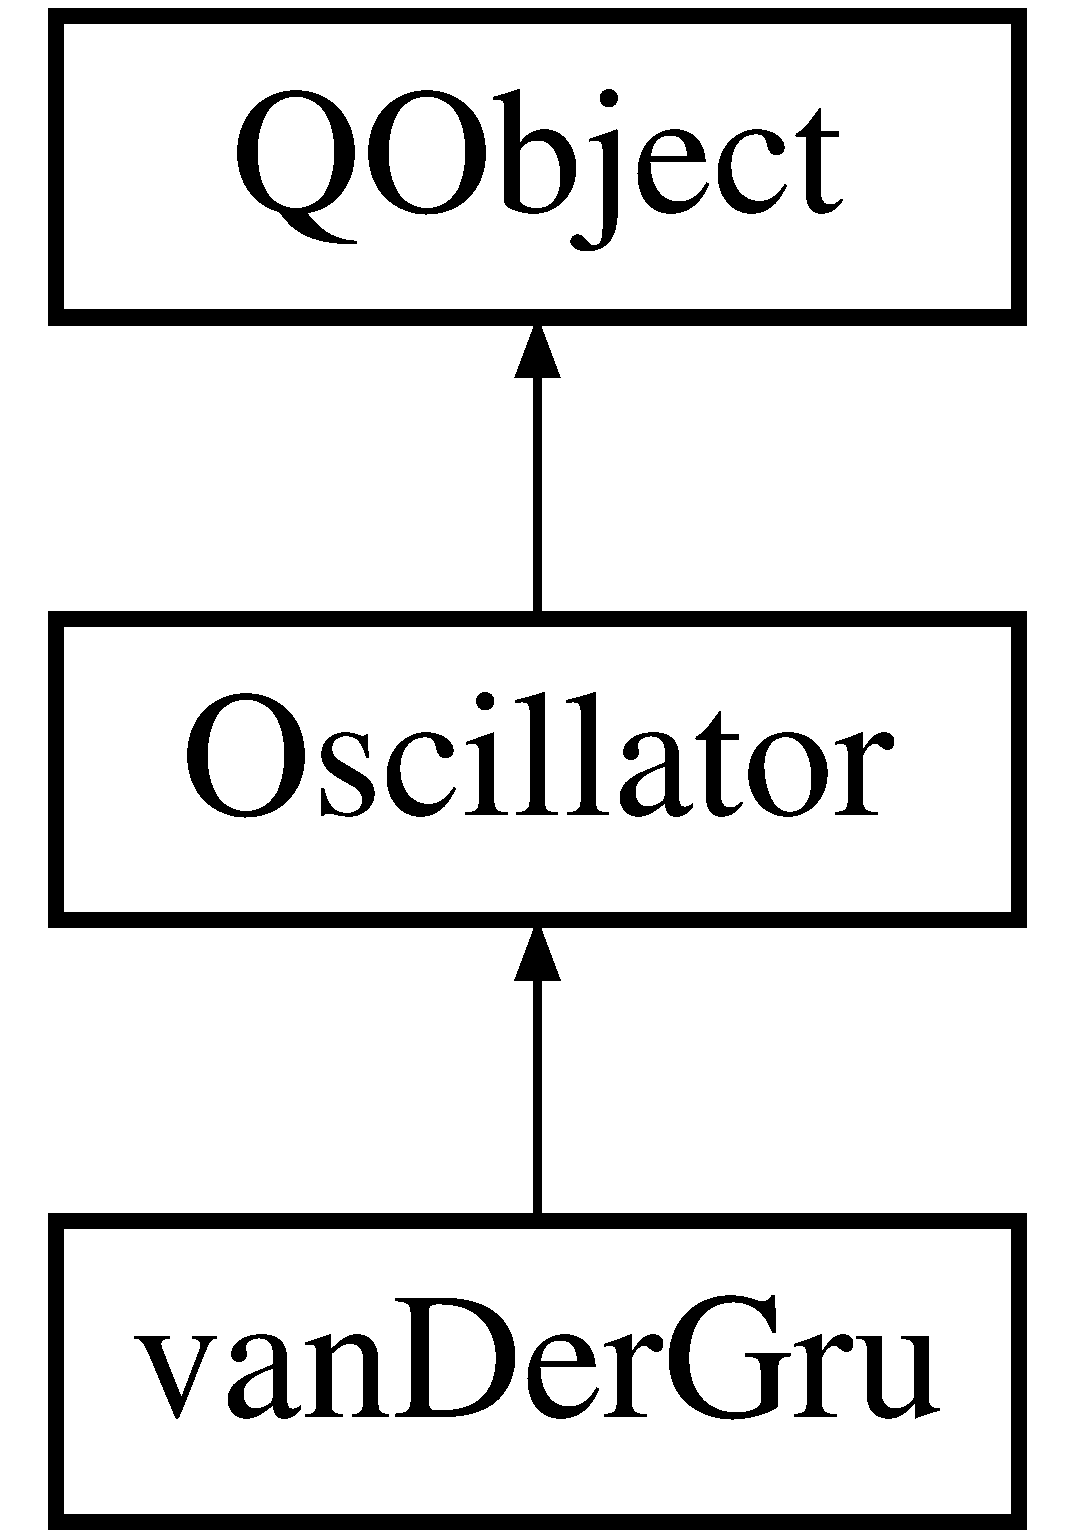
\includegraphics[height=3.000000cm]{classvan_der_gru}
\end{center}
\end{figure}
\subsection*{Public Slots}
\begin{DoxyCompactItemize}
\item 
void \hyperlink{classvan_der_gru_a7f23f10c78105ec2821acf928db7785d}{set\+Parameter} (double value, \hyperlink{heart_defines_8h_a79395aba577c2bc57e7ca211ff3476a6}{O\+S\+C\+\_\+\+P\+A\+R\+A\+M\+E\+T\+E\+R} parameter)
\item 
void \hyperlink{classvan_der_gru_a4be827aa1f0c024551f214aaa18cdd2e}{set\+Value\+Alpha} (double value)
\item 
void \hyperlink{classvan_der_gru_a48bf636ecb611cb6e763cc25370e6635}{set\+Value\+F} (double value)
\item 
void \hyperlink{classvan_der_gru_a0336d6c2ff3cd05535ed2e9c23b71dd8}{set\+Value\+D} (double value)
\item 
void \hyperlink{classvan_der_gru_a858d11b40253534ea8602471dc09e22b}{set\+Value\+E} (double value)
\item 
void \hyperlink{classvan_der_gru_a82f8824f96b8a8d18ae8c5fcda0a2121}{set\+Value\+V1} (double value)
\item 
void \hyperlink{classvan_der_gru_a11eabc477ff53a702cfcca3cceab6af3}{set\+Value\+V2} (double value)
\end{DoxyCompactItemize}
\subsection*{Signals}
\begin{DoxyCompactItemize}
\item 
void \hyperlink{classvan_der_gru_ae8e3c263e0bdd6f6768d9592c24917a6}{value\+Alpha\+Changed} (double new\+Value)
\end{DoxyCompactItemize}
\subsection*{Public Member Functions}
\begin{DoxyCompactItemize}
\item 
\hyperlink{classvan_der_gru_a3a61378605ee63c899a671919b3ef87f}{van\+Der\+Gru} (void)
\item 
\hyperlink{classvan_der_gru_af9ce49799c6bbe6825acfb0a16ecf847}{$\sim$van\+Der\+Gru} (void)
\item 
double \hyperlink{classvan_der_gru_ad80161e6f6b1ec07f8f806efe135a1a9}{van\+Der\+Gru\+Function} (double potential, double current)
\item 
double \hyperlink{classvan_der_gru_a42d35dfb23bb6306394e6fd4943db6f9}{get\+Current\+Prim} (int which)
\item 
double \hyperlink{classvan_der_gru_afe764c0c671b5a1f7cbf21f87f5eb936}{get\+Potential\+Prim} ()
\item 
void \hyperlink{classvan_der_gru_ac756d19f03e7387f09e94b27aff03da2}{set\+Default\+Av\+Parameters} ()
\end{DoxyCompactItemize}
\subsection*{Additional Inherited Members}


\subsection{Constructor \& Destructor Documentation}
\hypertarget{classvan_der_gru_a3a61378605ee63c899a671919b3ef87f}{\index{van\+Der\+Gru@{van\+Der\+Gru}!van\+Der\+Gru@{van\+Der\+Gru}}
\index{van\+Der\+Gru@{van\+Der\+Gru}!van\+Der\+Gru@{van\+Der\+Gru}}
\subsubsection[{van\+Der\+Gru}]{\setlength{\rightskip}{0pt plus 5cm}van\+Der\+Gru\+::van\+Der\+Gru (
\begin{DoxyParamCaption}
\item[{void}]{}
\end{DoxyParamCaption}
)}}\label{classvan_der_gru_a3a61378605ee63c899a671919b3ef87f}
\hypertarget{classvan_der_gru_af9ce49799c6bbe6825acfb0a16ecf847}{\index{van\+Der\+Gru@{van\+Der\+Gru}!````~van\+Der\+Gru@{$\sim$van\+Der\+Gru}}
\index{````~van\+Der\+Gru@{$\sim$van\+Der\+Gru}!van\+Der\+Gru@{van\+Der\+Gru}}
\subsubsection[{$\sim$van\+Der\+Gru}]{\setlength{\rightskip}{0pt plus 5cm}van\+Der\+Gru\+::$\sim$van\+Der\+Gru (
\begin{DoxyParamCaption}
\item[{void}]{}
\end{DoxyParamCaption}
)}}\label{classvan_der_gru_af9ce49799c6bbe6825acfb0a16ecf847}


\subsection{Member Function Documentation}
\hypertarget{classvan_der_gru_a42d35dfb23bb6306394e6fd4943db6f9}{\index{van\+Der\+Gru@{van\+Der\+Gru}!get\+Current\+Prim@{get\+Current\+Prim}}
\index{get\+Current\+Prim@{get\+Current\+Prim}!van\+Der\+Gru@{van\+Der\+Gru}}
\subsubsection[{get\+Current\+Prim}]{\setlength{\rightskip}{0pt plus 5cm}double van\+Der\+Gru\+::get\+Current\+Prim (
\begin{DoxyParamCaption}
\item[{int}]{which}
\end{DoxyParamCaption}
)}}\label{classvan_der_gru_a42d35dfb23bb6306394e6fd4943db6f9}
\hypertarget{classvan_der_gru_afe764c0c671b5a1f7cbf21f87f5eb936}{\index{van\+Der\+Gru@{van\+Der\+Gru}!get\+Potential\+Prim@{get\+Potential\+Prim}}
\index{get\+Potential\+Prim@{get\+Potential\+Prim}!van\+Der\+Gru@{van\+Der\+Gru}}
\subsubsection[{get\+Potential\+Prim}]{\setlength{\rightskip}{0pt plus 5cm}double van\+Der\+Gru\+::get\+Potential\+Prim (
\begin{DoxyParamCaption}
{}
\end{DoxyParamCaption}
)\hspace{0.3cm}{\ttfamily [virtual]}}}\label{classvan_der_gru_afe764c0c671b5a1f7cbf21f87f5eb936}


Reimplemented from \hyperlink{class_oscillator_a932fda2705d851fbe28c569547f4b4f1}{Oscillator}.

\hypertarget{classvan_der_gru_ac756d19f03e7387f09e94b27aff03da2}{\index{van\+Der\+Gru@{van\+Der\+Gru}!set\+Default\+Av\+Parameters@{set\+Default\+Av\+Parameters}}
\index{set\+Default\+Av\+Parameters@{set\+Default\+Av\+Parameters}!van\+Der\+Gru@{van\+Der\+Gru}}
\subsubsection[{set\+Default\+Av\+Parameters}]{\setlength{\rightskip}{0pt plus 5cm}void van\+Der\+Gru\+::set\+Default\+Av\+Parameters (
\begin{DoxyParamCaption}
{}
\end{DoxyParamCaption}
)}}\label{classvan_der_gru_ac756d19f03e7387f09e94b27aff03da2}
\hypertarget{classvan_der_gru_a7f23f10c78105ec2821acf928db7785d}{\index{van\+Der\+Gru@{van\+Der\+Gru}!set\+Parameter@{set\+Parameter}}
\index{set\+Parameter@{set\+Parameter}!van\+Der\+Gru@{van\+Der\+Gru}}
\subsubsection[{set\+Parameter}]{\setlength{\rightskip}{0pt plus 5cm}void van\+Der\+Gru\+::set\+Parameter (
\begin{DoxyParamCaption}
\item[{double}]{value, }
\item[{{\bf O\+S\+C\+\_\+\+P\+A\+R\+A\+M\+E\+T\+E\+R}}]{parameter}
\end{DoxyParamCaption}
)\hspace{0.3cm}{\ttfamily [slot]}}}\label{classvan_der_gru_a7f23f10c78105ec2821acf928db7785d}
\hypertarget{classvan_der_gru_a4be827aa1f0c024551f214aaa18cdd2e}{\index{van\+Der\+Gru@{van\+Der\+Gru}!set\+Value\+Alpha@{set\+Value\+Alpha}}
\index{set\+Value\+Alpha@{set\+Value\+Alpha}!van\+Der\+Gru@{van\+Der\+Gru}}
\subsubsection[{set\+Value\+Alpha}]{\setlength{\rightskip}{0pt plus 5cm}void van\+Der\+Gru\+::set\+Value\+Alpha (
\begin{DoxyParamCaption}
\item[{double}]{value}
\end{DoxyParamCaption}
)\hspace{0.3cm}{\ttfamily [slot]}}}\label{classvan_der_gru_a4be827aa1f0c024551f214aaa18cdd2e}
\hypertarget{classvan_der_gru_a0336d6c2ff3cd05535ed2e9c23b71dd8}{\index{van\+Der\+Gru@{van\+Der\+Gru}!set\+Value\+D@{set\+Value\+D}}
\index{set\+Value\+D@{set\+Value\+D}!van\+Der\+Gru@{van\+Der\+Gru}}
\subsubsection[{set\+Value\+D}]{\setlength{\rightskip}{0pt plus 5cm}void van\+Der\+Gru\+::set\+Value\+D (
\begin{DoxyParamCaption}
\item[{double}]{value}
\end{DoxyParamCaption}
)\hspace{0.3cm}{\ttfamily [slot]}}}\label{classvan_der_gru_a0336d6c2ff3cd05535ed2e9c23b71dd8}
\hypertarget{classvan_der_gru_a858d11b40253534ea8602471dc09e22b}{\index{van\+Der\+Gru@{van\+Der\+Gru}!set\+Value\+E@{set\+Value\+E}}
\index{set\+Value\+E@{set\+Value\+E}!van\+Der\+Gru@{van\+Der\+Gru}}
\subsubsection[{set\+Value\+E}]{\setlength{\rightskip}{0pt plus 5cm}void van\+Der\+Gru\+::set\+Value\+E (
\begin{DoxyParamCaption}
\item[{double}]{value}
\end{DoxyParamCaption}
)\hspace{0.3cm}{\ttfamily [slot]}}}\label{classvan_der_gru_a858d11b40253534ea8602471dc09e22b}
\hypertarget{classvan_der_gru_a48bf636ecb611cb6e763cc25370e6635}{\index{van\+Der\+Gru@{van\+Der\+Gru}!set\+Value\+F@{set\+Value\+F}}
\index{set\+Value\+F@{set\+Value\+F}!van\+Der\+Gru@{van\+Der\+Gru}}
\subsubsection[{set\+Value\+F}]{\setlength{\rightskip}{0pt plus 5cm}void van\+Der\+Gru\+::set\+Value\+F (
\begin{DoxyParamCaption}
\item[{double}]{value}
\end{DoxyParamCaption}
)\hspace{0.3cm}{\ttfamily [slot]}}}\label{classvan_der_gru_a48bf636ecb611cb6e763cc25370e6635}
\hypertarget{classvan_der_gru_a82f8824f96b8a8d18ae8c5fcda0a2121}{\index{van\+Der\+Gru@{van\+Der\+Gru}!set\+Value\+V1@{set\+Value\+V1}}
\index{set\+Value\+V1@{set\+Value\+V1}!van\+Der\+Gru@{van\+Der\+Gru}}
\subsubsection[{set\+Value\+V1}]{\setlength{\rightskip}{0pt plus 5cm}void van\+Der\+Gru\+::set\+Value\+V1 (
\begin{DoxyParamCaption}
\item[{double}]{value}
\end{DoxyParamCaption}
)\hspace{0.3cm}{\ttfamily [slot]}}}\label{classvan_der_gru_a82f8824f96b8a8d18ae8c5fcda0a2121}
\hypertarget{classvan_der_gru_a11eabc477ff53a702cfcca3cceab6af3}{\index{van\+Der\+Gru@{van\+Der\+Gru}!set\+Value\+V2@{set\+Value\+V2}}
\index{set\+Value\+V2@{set\+Value\+V2}!van\+Der\+Gru@{van\+Der\+Gru}}
\subsubsection[{set\+Value\+V2}]{\setlength{\rightskip}{0pt plus 5cm}void van\+Der\+Gru\+::set\+Value\+V2 (
\begin{DoxyParamCaption}
\item[{double}]{value}
\end{DoxyParamCaption}
)\hspace{0.3cm}{\ttfamily [slot]}}}\label{classvan_der_gru_a11eabc477ff53a702cfcca3cceab6af3}
\hypertarget{classvan_der_gru_ae8e3c263e0bdd6f6768d9592c24917a6}{\index{van\+Der\+Gru@{van\+Der\+Gru}!value\+Alpha\+Changed@{value\+Alpha\+Changed}}
\index{value\+Alpha\+Changed@{value\+Alpha\+Changed}!van\+Der\+Gru@{van\+Der\+Gru}}
\subsubsection[{value\+Alpha\+Changed}]{\setlength{\rightskip}{0pt plus 5cm}void van\+Der\+Gru\+::value\+Alpha\+Changed (
\begin{DoxyParamCaption}
\item[{double}]{new\+Value}
\end{DoxyParamCaption}
)\hspace{0.3cm}{\ttfamily [signal]}}}\label{classvan_der_gru_ae8e3c263e0bdd6f6768d9592c24917a6}
\hypertarget{classvan_der_gru_ad80161e6f6b1ec07f8f806efe135a1a9}{\index{van\+Der\+Gru@{van\+Der\+Gru}!van\+Der\+Gru\+Function@{van\+Der\+Gru\+Function}}
\index{van\+Der\+Gru\+Function@{van\+Der\+Gru\+Function}!van\+Der\+Gru@{van\+Der\+Gru}}
\subsubsection[{van\+Der\+Gru\+Function}]{\setlength{\rightskip}{0pt plus 5cm}double van\+Der\+Gru\+::van\+Der\+Gru\+Function (
\begin{DoxyParamCaption}
\item[{double}]{potential, }
\item[{double}]{current}
\end{DoxyParamCaption}
)}}\label{classvan_der_gru_ad80161e6f6b1ec07f8f806efe135a1a9}


The documentation for this class was generated from the following files\+:\begin{DoxyCompactItemize}
\item 
Model/\hyperlink{van_der_gru_8h}{van\+Der\+Gru.\+h}\item 
Model/\hyperlink{van_der_gru_8cpp}{van\+Der\+Gru.\+cpp}\end{DoxyCompactItemize}

\chapter{File Documentation}
\hypertarget{_atrial_machine2d_8cpp}{\section{Atrial\+Machine2d.\+cpp File Reference}
\label{_atrial_machine2d_8cpp}\index{Atrial\+Machine2d.\+cpp@{Atrial\+Machine2d.\+cpp}}
}
{\ttfamily \#include \char`\"{}Atrial\+Machine2d.\+h\char`\"{}}\\*
{\ttfamily \#include \char`\"{}Numeric\+Strategy\textbackslash{}\+Forward\+Euler\+Strategy.\+h\char`\"{}}\\*
{\ttfamily \#include \char`\"{}Numeric\+Strategy\textbackslash{}\+Allexandre\+Strategy.\+h\char`\"{}}\\*
\subsection*{Macros}
\begin{DoxyCompactItemize}
\item 
\#define \hyperlink{_atrial_machine2d_8cpp_ab2d1a3e2009d55abc0f7134238c2d17b}{E\+L\+E\+C\+T\+R\+O\+G\+R\+A\+M\+M\+M}~1
\end{DoxyCompactItemize}


\subsection{Macro Definition Documentation}
\hypertarget{_atrial_machine2d_8cpp_ab2d1a3e2009d55abc0f7134238c2d17b}{\index{Atrial\+Machine2d.\+cpp@{Atrial\+Machine2d.\+cpp}!E\+L\+E\+C\+T\+R\+O\+G\+R\+A\+M\+M\+M@{E\+L\+E\+C\+T\+R\+O\+G\+R\+A\+M\+M\+M}}
\index{E\+L\+E\+C\+T\+R\+O\+G\+R\+A\+M\+M\+M@{E\+L\+E\+C\+T\+R\+O\+G\+R\+A\+M\+M\+M}!Atrial\+Machine2d.\+cpp@{Atrial\+Machine2d.\+cpp}}
\subsubsection[{E\+L\+E\+C\+T\+R\+O\+G\+R\+A\+M\+M\+M}]{\setlength{\rightskip}{0pt plus 5cm}\#define E\+L\+E\+C\+T\+R\+O\+G\+R\+A\+M\+M\+M~1}}\label{_atrial_machine2d_8cpp_ab2d1a3e2009d55abc0f7134238c2d17b}

\hypertarget{_atrial_machine2d_8h}{\section{Atrial\+Machine2d.\+h File Reference}
\label{_atrial_machine2d_8h}\index{Atrial\+Machine2d.\+h@{Atrial\+Machine2d.\+h}}
}
{\ttfamily \#include $<$Q\+Object$>$}\\*
{\ttfamily \#include $<$vector$>$}\\*
{\ttfamily \#include $<$cmath$>$}\\*
{\ttfamily \#include $<$Qt\+Gui/\+Q\+Message\+Box$>$}\\*
{\ttfamily \#include \char`\"{}R\+Rcalculator.\+h\char`\"{}}\\*
{\ttfamily \#include \char`\"{}Model\textbackslash{}\+Oscillator.\+h\char`\"{}}\\*
{\ttfamily \#include \char`\"{}Model\textbackslash{}van\+Der\+Gru.\+h\char`\"{}}\\*
{\ttfamily \#include \char`\"{}Model\textbackslash{}v3model.\+h\char`\"{}}\\*
{\ttfamily \#include \char`\"{}Model\textbackslash{}\+Fitz\+Hugh\+Nagumo.\+h\char`\"{}}\\*
{\ttfamily \#include $<$fstream$>$}\\*
{\ttfamily \#include $<$ctime$>$}\\*
{\ttfamily \#include $<$sstream$>$}\\*
{\ttfamily \#include \char`\"{}Random\+Generator.\+h\char`\"{}}\\*
{\ttfamily \#include \char`\"{}atrial\+Parameters.\+h\char`\"{}}\\*
{\ttfamily \#include \char`\"{}Model\textbackslash{}\+Cardiac\+Mesh.\+h\char`\"{}}\\*
{\ttfamily \#include \char`\"{}Numeric\+Strategy\textbackslash{}\+Numeric\+Strategy.\+h\char`\"{}}\\*
\subsection*{Classes}
\begin{DoxyCompactItemize}
\item 
class \hyperlink{classburster}{burster}
\item 
class \hyperlink{class_atrial_machine2d}{Atrial\+Machine2d}
\end{DoxyCompactItemize}

\hypertarget{atrial_parameters_8cpp}{\section{atrial\+Parameters.\+cpp File Reference}
\label{atrial_parameters_8cpp}\index{atrial\+Parameters.\+cpp@{atrial\+Parameters.\+cpp}}
}
{\ttfamily \#include \char`\"{}atrial\+Parameters.\+h\char`\"{}}\\*

\hypertarget{atrial_parameters_8h}{\section{atrial\+Parameters.\+h File Reference}
\label{atrial_parameters_8h}\index{atrial\+Parameters.\+h@{atrial\+Parameters.\+h}}
}
{\ttfamily \#include \char`\"{}heart\+Defines.\+h\char`\"{}}\\*
\subsection*{Classes}
\begin{DoxyCompactItemize}
\item 
class \hyperlink{classatrial_parameters}{atrial\+Parameters}
\end{DoxyCompactItemize}

\hypertarget{_curve_data_8cpp}{\section{Curve\+Data.\+cpp File Reference}
\label{_curve_data_8cpp}\index{Curve\+Data.\+cpp@{Curve\+Data.\+cpp}}
}
{\ttfamily \#include \char`\"{}Curve\+Data.\+h\char`\"{}}\\*

\hypertarget{_curve_data_8h}{\section{Curve\+Data.\+h File Reference}
\label{_curve_data_8h}\index{Curve\+Data.\+h@{Curve\+Data.\+h}}
}
{\ttfamily \#include $<$vector$>$}\\*
\subsection*{Classes}
\begin{DoxyCompactItemize}
\item 
class \hyperlink{class_curve_data}{Curve\+Data}
\end{DoxyCompactItemize}

\hypertarget{default_plot_8cpp}{\section{default\+Plot.\+cpp File Reference}
\label{default_plot_8cpp}\index{default\+Plot.\+cpp@{default\+Plot.\+cpp}}
}
{\ttfamily \#include $<$qwt\+\_\+math.\+h$>$}\\*
{\ttfamily \#include $<$qwt\+\_\+symbol.\+h$>$}\\*
{\ttfamily \#include $<$qwt\+\_\+picker\+\_\+machine.\+h$>$}\\*
{\ttfamily \#include $<$qwt\+\_\+plot\+\_\+canvas.\+h$>$}\\*
{\ttfamily \#include $<$qwt\+\_\+text.\+h$>$}\\*
{\ttfamily \#include \char`\"{}default\+Plot.\+h\char`\"{}}\\*
\subsection*{Functions}
\begin{DoxyCompactItemize}
\item 
Q\+Font \hyperlink{default_plot_8cpp_a3c18e4b03e63db29d5428b786dc959eb}{g\+\_\+axis\+Font} (\char`\"{}Times\char`\"{}, 7)
\item 
Q\+Font \hyperlink{default_plot_8cpp_aa188aa0890ed106421b705974e0fa283}{g\+\_\+legends\+Font} (\char`\"{}Times\char`\"{}, 7)
\item 
Q\+Font \hyperlink{default_plot_8cpp_a208d70248f891a6c5efe08e38571456b}{g\+\_\+title\+Font} (\char`\"{}Times\char`\"{}, 7)
\end{DoxyCompactItemize}


\subsection{Function Documentation}
\hypertarget{default_plot_8cpp_a3c18e4b03e63db29d5428b786dc959eb}{\index{default\+Plot.\+cpp@{default\+Plot.\+cpp}!g\+\_\+axis\+Font@{g\+\_\+axis\+Font}}
\index{g\+\_\+axis\+Font@{g\+\_\+axis\+Font}!default\+Plot.\+cpp@{default\+Plot.\+cpp}}
\subsubsection[{g\+\_\+axis\+Font}]{\setlength{\rightskip}{0pt plus 5cm}Q\+Font g\+\_\+axis\+Font (
\begin{DoxyParamCaption}
\item[{\char`\"{}Times\char`\"{}}]{, }
\item[{7}]{}
\end{DoxyParamCaption}
)}}\label{default_plot_8cpp_a3c18e4b03e63db29d5428b786dc959eb}
\hypertarget{default_plot_8cpp_aa188aa0890ed106421b705974e0fa283}{\index{default\+Plot.\+cpp@{default\+Plot.\+cpp}!g\+\_\+legends\+Font@{g\+\_\+legends\+Font}}
\index{g\+\_\+legends\+Font@{g\+\_\+legends\+Font}!default\+Plot.\+cpp@{default\+Plot.\+cpp}}
\subsubsection[{g\+\_\+legends\+Font}]{\setlength{\rightskip}{0pt plus 5cm}Q\+Font g\+\_\+legends\+Font (
\begin{DoxyParamCaption}
\item[{\char`\"{}Times\char`\"{}}]{, }
\item[{7}]{}
\end{DoxyParamCaption}
)}}\label{default_plot_8cpp_aa188aa0890ed106421b705974e0fa283}
\hypertarget{default_plot_8cpp_a208d70248f891a6c5efe08e38571456b}{\index{default\+Plot.\+cpp@{default\+Plot.\+cpp}!g\+\_\+title\+Font@{g\+\_\+title\+Font}}
\index{g\+\_\+title\+Font@{g\+\_\+title\+Font}!default\+Plot.\+cpp@{default\+Plot.\+cpp}}
\subsubsection[{g\+\_\+title\+Font}]{\setlength{\rightskip}{0pt plus 5cm}Q\+Font g\+\_\+title\+Font (
\begin{DoxyParamCaption}
\item[{\char`\"{}Times\char`\"{}}]{, }
\item[{7}]{}
\end{DoxyParamCaption}
)}}\label{default_plot_8cpp_a208d70248f891a6c5efe08e38571456b}

\hypertarget{default_plot_8h}{\section{default\+Plot.\+h File Reference}
\label{default_plot_8h}\index{default\+Plot.\+h@{default\+Plot.\+h}}
}
{\ttfamily \#include $<$qwt\+\_\+plot.\+h$>$}\\*
{\ttfamily \#include $<$qwt\+\_\+plot\+\_\+grid.\+h$>$}\\*
{\ttfamily \#include $<$qwt\+\_\+plot\+\_\+layout.\+h$>$}\\*
{\ttfamily \#include $<$qwt\+\_\+plot\+\_\+zoomer.\+h$>$}\\*
{\ttfamily \#include $<$qwt\+\_\+legend.\+h$>$}\\*
{\ttfamily \#include \char`\"{}Curve\+Data.\+h\char`\"{}}\\*
{\ttfamily \#include \char`\"{}heart\+Defines.\+h\char`\"{}}\\*
{\ttfamily \#include \char`\"{}atrial\+Parameters.\+h\char`\"{}}\\*
{\ttfamily \#include $<$vector$>$}\\*
{\ttfamily \#include $<$string$>$}\\*
{\ttfamily \#include $<$qwt\+\_\+scale\+\_\+widget.\+h$>$}\\*
{\ttfamily \#include $<$qwt\+\_\+plot\+\_\+marker.\+h$>$}\\*
{\ttfamily \#include $<$qwt\+\_\+plot\+\_\+curve.\+h$>$}\\*
{\ttfamily \#include $<$qwt\+\_\+painter.\+h$>$}\\*
{\ttfamily \#include $<$qwt\+\_\+plot\+\_\+canvas.\+h$>$}\\*
{\ttfamily \#include $<$Qt\+Gui$>$}\\*
\subsection*{Classes}
\begin{DoxyCompactItemize}
\item 
class \hyperlink{class_default_plot}{Default\+Plot}
\end{DoxyCompactItemize}

\hypertarget{_diffusion_matrix_8cpp}{\section{Diffusion\+Matrix.\+cpp File Reference}
\label{_diffusion_matrix_8cpp}\index{Diffusion\+Matrix.\+cpp@{Diffusion\+Matrix.\+cpp}}
}
{\ttfamily \#include \char`\"{}Diffusion\+Matrix.\+h\char`\"{}}\\*

\hypertarget{_diffusion_matrix_8h}{\section{Diffusion\+Matrix.\+h File Reference}
\label{_diffusion_matrix_8h}\index{Diffusion\+Matrix.\+h@{Diffusion\+Matrix.\+h}}
}
{\ttfamily \#include $<$Q\+Color$>$}\\*
{\ttfamily \#include $<$Q\+Point$>$}\\*
{\ttfamily \#include $<$vector$>$}\\*
{\ttfamily \#include \char`\"{}heart\+Defines.\+h\char`\"{}}\\*
{\ttfamily \#include \char`\"{}Model\textbackslash{}cartesian\+Grid.\+h\char`\"{}}\\*
{\ttfamily \#include \char`\"{}Model\textbackslash{}\+Cardiac\+Mesh.\+h\char`\"{}}\\*
\subsection*{Classes}
\begin{DoxyCompactItemize}
\item 
class \hyperlink{class_pix}{Pix}
\item 
class \hyperlink{class_diffusion_matrix}{Diffusion\+Matrix}
\end{DoxyCompactItemize}

\hypertarget{_diffusion_painter_8cpp}{\section{Diffusion\+Painter.\+cpp File Reference}
\label{_diffusion_painter_8cpp}\index{Diffusion\+Painter.\+cpp@{Diffusion\+Painter.\+cpp}}
}
{\ttfamily \#include $<$Qt\+Gui$>$}\\*
{\ttfamily \#include $<$Qt\+Open\+G\+L$>$}\\*
{\ttfamily \#include $<$math.\+h$>$}\\*
{\ttfamily \#include \char`\"{}Diffusion\+Painter.\+h\char`\"{}}\\*
\subsection*{Macros}
\begin{DoxyCompactItemize}
\item 
\#define \hyperlink{_diffusion_painter_8cpp_aa2b6486ff7ecee8bf04e3371f197527a}{G\+L\+\_\+\+M\+U\+L\+T\+I\+S\+A\+M\+P\+L\+E}~0x809\+D
\end{DoxyCompactItemize}


\subsection{Macro Definition Documentation}
\hypertarget{_diffusion_painter_8cpp_aa2b6486ff7ecee8bf04e3371f197527a}{\index{Diffusion\+Painter.\+cpp@{Diffusion\+Painter.\+cpp}!G\+L\+\_\+\+M\+U\+L\+T\+I\+S\+A\+M\+P\+L\+E@{G\+L\+\_\+\+M\+U\+L\+T\+I\+S\+A\+M\+P\+L\+E}}
\index{G\+L\+\_\+\+M\+U\+L\+T\+I\+S\+A\+M\+P\+L\+E@{G\+L\+\_\+\+M\+U\+L\+T\+I\+S\+A\+M\+P\+L\+E}!Diffusion\+Painter.\+cpp@{Diffusion\+Painter.\+cpp}}
\subsubsection[{G\+L\+\_\+\+M\+U\+L\+T\+I\+S\+A\+M\+P\+L\+E}]{\setlength{\rightskip}{0pt plus 5cm}\#define G\+L\+\_\+\+M\+U\+L\+T\+I\+S\+A\+M\+P\+L\+E~0x809\+D}}\label{_diffusion_painter_8cpp_aa2b6486ff7ecee8bf04e3371f197527a}

\hypertarget{_diffusion_painter_8h}{\section{Diffusion\+Painter.\+h File Reference}
\label{_diffusion_painter_8h}\index{Diffusion\+Painter.\+h@{Diffusion\+Painter.\+h}}
}
{\ttfamily \#include $<$Q\+G\+L\+Widget$>$}\\*
{\ttfamily \#include \char`\"{}Probe.\+h\char`\"{}}\\*
{\ttfamily \#include \char`\"{}heart\+Defines.\+h\char`\"{}}\\*
{\ttfamily \#include \char`\"{}Model\textbackslash{}cartesian\+Grid.\+h\char`\"{}}\\*
{\ttfamily \#include \char`\"{}Random\+Generator.\+h\char`\"{}}\\*
{\ttfamily \#include \char`\"{}Diffusion\+Matrix.\+h\char`\"{}}\\*
{\ttfamily \#include \char`\"{}Model\textbackslash{}\+Cardiac\+Mesh.\+h\char`\"{}}\\*
{\ttfamily \#include \char`\"{}G\+Lfunc.\+h\char`\"{}}\\*
{\ttfamily \#include $<$assert.\+h$>$}\\*
\subsection*{Classes}
\begin{DoxyCompactItemize}
\item 
class \hyperlink{class_diffusion_painter}{Diffusion\+Painter}
\end{DoxyCompactItemize}

\hypertarget{fastonebigheader_8h}{\section{fastonebigheader.\+h File Reference}
\label{fastonebigheader_8h}\index{fastonebigheader.\+h@{fastonebigheader.\+h}}
}
{\ttfamily \#include $<$stdint.\+h$>$}\\*
{\ttfamily \#include $<$math.\+h$>$}\\*
\subsection*{Macros}
\begin{DoxyCompactItemize}
\item 
\#define \hyperlink{fastonebigheader_8h_a676fea0678945be0b1da32705b938e1a}{cast\+\_\+uint32\+\_\+t}~(uint32\+\_\+t)
\item 
\#define \hyperlink{fastonebigheader_8h_aeddf845aafcd1eca2c464038d60107eb}{\+\_\+\+\_\+\+F\+A\+S\+T\+\_\+\+E\+X\+P\+\_\+\+H\+\_\+}
\item 
\#define \hyperlink{fastonebigheader_8h_a839d9b4ce15cd3e43ed4e56923edace0}{\+\_\+\+\_\+\+F\+A\+S\+T\+\_\+\+L\+O\+G\+\_\+\+H\+\_\+}
\item 
\#define \hyperlink{fastonebigheader_8h_a58750005e14fb2e0b1f672811dfb75de}{\+\_\+\+\_\+\+F\+A\+S\+T\+\_\+\+E\+R\+F\+\_\+\+H\+\_\+}
\item 
\#define \hyperlink{fastonebigheader_8h_aae16f962a2438e8a36a7349fc654c364}{\+\_\+\+\_\+\+F\+A\+S\+T\+\_\+\+G\+A\+M\+M\+A\+\_\+\+H\+\_\+}
\item 
\#define \hyperlink{fastonebigheader_8h_a498423e4e94b00fbe9c89d8d33b77796}{\+\_\+\+\_\+\+F\+A\+S\+T\+\_\+\+H\+Y\+P\+E\+R\+B\+O\+L\+I\+C\+\_\+\+H\+\_\+}
\item 
\#define \hyperlink{fastonebigheader_8h_aa2abf33d605c5988517d6bfcea219abe}{\+\_\+\+\_\+\+F\+A\+S\+T\+\_\+\+L\+A\+M\+B\+E\+R\+T\+\_\+\+W\+\_\+\+H\+\_\+}
\item 
\#define \hyperlink{fastonebigheader_8h_a2d62c30ae38d88436fb731dbf0bd18d5}{\+\_\+\+\_\+\+F\+A\+S\+T\+\_\+\+P\+O\+W\+\_\+\+H\+\_\+}
\item 
\#define \hyperlink{fastonebigheader_8h_ae1b85b5312e952a349945ce85c374b80}{\+\_\+\+\_\+\+F\+A\+S\+T\+\_\+\+S\+I\+G\+M\+O\+I\+D\+\_\+\+H\+\_\+}
\item 
\#define \hyperlink{fastonebigheader_8h_a63ebb09d456fe33fcdcc93104447a841}{\+\_\+\+\_\+\+F\+A\+S\+T\+\_\+\+T\+R\+I\+G\+\_\+\+H\+\_\+}
\end{DoxyCompactItemize}


\subsection{Macro Definition Documentation}
\hypertarget{fastonebigheader_8h_a58750005e14fb2e0b1f672811dfb75de}{\index{fastonebigheader.\+h@{fastonebigheader.\+h}!\+\_\+\+\_\+\+F\+A\+S\+T\+\_\+\+E\+R\+F\+\_\+\+H\+\_\+@{\+\_\+\+\_\+\+F\+A\+S\+T\+\_\+\+E\+R\+F\+\_\+\+H\+\_\+}}
\index{\+\_\+\+\_\+\+F\+A\+S\+T\+\_\+\+E\+R\+F\+\_\+\+H\+\_\+@{\+\_\+\+\_\+\+F\+A\+S\+T\+\_\+\+E\+R\+F\+\_\+\+H\+\_\+}!fastonebigheader.\+h@{fastonebigheader.\+h}}
\subsubsection[{\+\_\+\+\_\+\+F\+A\+S\+T\+\_\+\+E\+R\+F\+\_\+\+H\+\_\+}]{\setlength{\rightskip}{0pt plus 5cm}\#define \+\_\+\+\_\+\+F\+A\+S\+T\+\_\+\+E\+R\+F\+\_\+\+H\+\_\+}}\label{fastonebigheader_8h_a58750005e14fb2e0b1f672811dfb75de}
\hypertarget{fastonebigheader_8h_aeddf845aafcd1eca2c464038d60107eb}{\index{fastonebigheader.\+h@{fastonebigheader.\+h}!\+\_\+\+\_\+\+F\+A\+S\+T\+\_\+\+E\+X\+P\+\_\+\+H\+\_\+@{\+\_\+\+\_\+\+F\+A\+S\+T\+\_\+\+E\+X\+P\+\_\+\+H\+\_\+}}
\index{\+\_\+\+\_\+\+F\+A\+S\+T\+\_\+\+E\+X\+P\+\_\+\+H\+\_\+@{\+\_\+\+\_\+\+F\+A\+S\+T\+\_\+\+E\+X\+P\+\_\+\+H\+\_\+}!fastonebigheader.\+h@{fastonebigheader.\+h}}
\subsubsection[{\+\_\+\+\_\+\+F\+A\+S\+T\+\_\+\+E\+X\+P\+\_\+\+H\+\_\+}]{\setlength{\rightskip}{0pt plus 5cm}\#define \+\_\+\+\_\+\+F\+A\+S\+T\+\_\+\+E\+X\+P\+\_\+\+H\+\_\+}}\label{fastonebigheader_8h_aeddf845aafcd1eca2c464038d60107eb}
\hypertarget{fastonebigheader_8h_aae16f962a2438e8a36a7349fc654c364}{\index{fastonebigheader.\+h@{fastonebigheader.\+h}!\+\_\+\+\_\+\+F\+A\+S\+T\+\_\+\+G\+A\+M\+M\+A\+\_\+\+H\+\_\+@{\+\_\+\+\_\+\+F\+A\+S\+T\+\_\+\+G\+A\+M\+M\+A\+\_\+\+H\+\_\+}}
\index{\+\_\+\+\_\+\+F\+A\+S\+T\+\_\+\+G\+A\+M\+M\+A\+\_\+\+H\+\_\+@{\+\_\+\+\_\+\+F\+A\+S\+T\+\_\+\+G\+A\+M\+M\+A\+\_\+\+H\+\_\+}!fastonebigheader.\+h@{fastonebigheader.\+h}}
\subsubsection[{\+\_\+\+\_\+\+F\+A\+S\+T\+\_\+\+G\+A\+M\+M\+A\+\_\+\+H\+\_\+}]{\setlength{\rightskip}{0pt plus 5cm}\#define \+\_\+\+\_\+\+F\+A\+S\+T\+\_\+\+G\+A\+M\+M\+A\+\_\+\+H\+\_\+}}\label{fastonebigheader_8h_aae16f962a2438e8a36a7349fc654c364}
\hypertarget{fastonebigheader_8h_a498423e4e94b00fbe9c89d8d33b77796}{\index{fastonebigheader.\+h@{fastonebigheader.\+h}!\+\_\+\+\_\+\+F\+A\+S\+T\+\_\+\+H\+Y\+P\+E\+R\+B\+O\+L\+I\+C\+\_\+\+H\+\_\+@{\+\_\+\+\_\+\+F\+A\+S\+T\+\_\+\+H\+Y\+P\+E\+R\+B\+O\+L\+I\+C\+\_\+\+H\+\_\+}}
\index{\+\_\+\+\_\+\+F\+A\+S\+T\+\_\+\+H\+Y\+P\+E\+R\+B\+O\+L\+I\+C\+\_\+\+H\+\_\+@{\+\_\+\+\_\+\+F\+A\+S\+T\+\_\+\+H\+Y\+P\+E\+R\+B\+O\+L\+I\+C\+\_\+\+H\+\_\+}!fastonebigheader.\+h@{fastonebigheader.\+h}}
\subsubsection[{\+\_\+\+\_\+\+F\+A\+S\+T\+\_\+\+H\+Y\+P\+E\+R\+B\+O\+L\+I\+C\+\_\+\+H\+\_\+}]{\setlength{\rightskip}{0pt plus 5cm}\#define \+\_\+\+\_\+\+F\+A\+S\+T\+\_\+\+H\+Y\+P\+E\+R\+B\+O\+L\+I\+C\+\_\+\+H\+\_\+}}\label{fastonebigheader_8h_a498423e4e94b00fbe9c89d8d33b77796}
\hypertarget{fastonebigheader_8h_aa2abf33d605c5988517d6bfcea219abe}{\index{fastonebigheader.\+h@{fastonebigheader.\+h}!\+\_\+\+\_\+\+F\+A\+S\+T\+\_\+\+L\+A\+M\+B\+E\+R\+T\+\_\+\+W\+\_\+\+H\+\_\+@{\+\_\+\+\_\+\+F\+A\+S\+T\+\_\+\+L\+A\+M\+B\+E\+R\+T\+\_\+\+W\+\_\+\+H\+\_\+}}
\index{\+\_\+\+\_\+\+F\+A\+S\+T\+\_\+\+L\+A\+M\+B\+E\+R\+T\+\_\+\+W\+\_\+\+H\+\_\+@{\+\_\+\+\_\+\+F\+A\+S\+T\+\_\+\+L\+A\+M\+B\+E\+R\+T\+\_\+\+W\+\_\+\+H\+\_\+}!fastonebigheader.\+h@{fastonebigheader.\+h}}
\subsubsection[{\+\_\+\+\_\+\+F\+A\+S\+T\+\_\+\+L\+A\+M\+B\+E\+R\+T\+\_\+\+W\+\_\+\+H\+\_\+}]{\setlength{\rightskip}{0pt plus 5cm}\#define \+\_\+\+\_\+\+F\+A\+S\+T\+\_\+\+L\+A\+M\+B\+E\+R\+T\+\_\+\+W\+\_\+\+H\+\_\+}}\label{fastonebigheader_8h_aa2abf33d605c5988517d6bfcea219abe}
\hypertarget{fastonebigheader_8h_a839d9b4ce15cd3e43ed4e56923edace0}{\index{fastonebigheader.\+h@{fastonebigheader.\+h}!\+\_\+\+\_\+\+F\+A\+S\+T\+\_\+\+L\+O\+G\+\_\+\+H\+\_\+@{\+\_\+\+\_\+\+F\+A\+S\+T\+\_\+\+L\+O\+G\+\_\+\+H\+\_\+}}
\index{\+\_\+\+\_\+\+F\+A\+S\+T\+\_\+\+L\+O\+G\+\_\+\+H\+\_\+@{\+\_\+\+\_\+\+F\+A\+S\+T\+\_\+\+L\+O\+G\+\_\+\+H\+\_\+}!fastonebigheader.\+h@{fastonebigheader.\+h}}
\subsubsection[{\+\_\+\+\_\+\+F\+A\+S\+T\+\_\+\+L\+O\+G\+\_\+\+H\+\_\+}]{\setlength{\rightskip}{0pt plus 5cm}\#define \+\_\+\+\_\+\+F\+A\+S\+T\+\_\+\+L\+O\+G\+\_\+\+H\+\_\+}}\label{fastonebigheader_8h_a839d9b4ce15cd3e43ed4e56923edace0}
\hypertarget{fastonebigheader_8h_a2d62c30ae38d88436fb731dbf0bd18d5}{\index{fastonebigheader.\+h@{fastonebigheader.\+h}!\+\_\+\+\_\+\+F\+A\+S\+T\+\_\+\+P\+O\+W\+\_\+\+H\+\_\+@{\+\_\+\+\_\+\+F\+A\+S\+T\+\_\+\+P\+O\+W\+\_\+\+H\+\_\+}}
\index{\+\_\+\+\_\+\+F\+A\+S\+T\+\_\+\+P\+O\+W\+\_\+\+H\+\_\+@{\+\_\+\+\_\+\+F\+A\+S\+T\+\_\+\+P\+O\+W\+\_\+\+H\+\_\+}!fastonebigheader.\+h@{fastonebigheader.\+h}}
\subsubsection[{\+\_\+\+\_\+\+F\+A\+S\+T\+\_\+\+P\+O\+W\+\_\+\+H\+\_\+}]{\setlength{\rightskip}{0pt plus 5cm}\#define \+\_\+\+\_\+\+F\+A\+S\+T\+\_\+\+P\+O\+W\+\_\+\+H\+\_\+}}\label{fastonebigheader_8h_a2d62c30ae38d88436fb731dbf0bd18d5}
\hypertarget{fastonebigheader_8h_ae1b85b5312e952a349945ce85c374b80}{\index{fastonebigheader.\+h@{fastonebigheader.\+h}!\+\_\+\+\_\+\+F\+A\+S\+T\+\_\+\+S\+I\+G\+M\+O\+I\+D\+\_\+\+H\+\_\+@{\+\_\+\+\_\+\+F\+A\+S\+T\+\_\+\+S\+I\+G\+M\+O\+I\+D\+\_\+\+H\+\_\+}}
\index{\+\_\+\+\_\+\+F\+A\+S\+T\+\_\+\+S\+I\+G\+M\+O\+I\+D\+\_\+\+H\+\_\+@{\+\_\+\+\_\+\+F\+A\+S\+T\+\_\+\+S\+I\+G\+M\+O\+I\+D\+\_\+\+H\+\_\+}!fastonebigheader.\+h@{fastonebigheader.\+h}}
\subsubsection[{\+\_\+\+\_\+\+F\+A\+S\+T\+\_\+\+S\+I\+G\+M\+O\+I\+D\+\_\+\+H\+\_\+}]{\setlength{\rightskip}{0pt plus 5cm}\#define \+\_\+\+\_\+\+F\+A\+S\+T\+\_\+\+S\+I\+G\+M\+O\+I\+D\+\_\+\+H\+\_\+}}\label{fastonebigheader_8h_ae1b85b5312e952a349945ce85c374b80}
\hypertarget{fastonebigheader_8h_a63ebb09d456fe33fcdcc93104447a841}{\index{fastonebigheader.\+h@{fastonebigheader.\+h}!\+\_\+\+\_\+\+F\+A\+S\+T\+\_\+\+T\+R\+I\+G\+\_\+\+H\+\_\+@{\+\_\+\+\_\+\+F\+A\+S\+T\+\_\+\+T\+R\+I\+G\+\_\+\+H\+\_\+}}
\index{\+\_\+\+\_\+\+F\+A\+S\+T\+\_\+\+T\+R\+I\+G\+\_\+\+H\+\_\+@{\+\_\+\+\_\+\+F\+A\+S\+T\+\_\+\+T\+R\+I\+G\+\_\+\+H\+\_\+}!fastonebigheader.\+h@{fastonebigheader.\+h}}
\subsubsection[{\+\_\+\+\_\+\+F\+A\+S\+T\+\_\+\+T\+R\+I\+G\+\_\+\+H\+\_\+}]{\setlength{\rightskip}{0pt plus 5cm}\#define \+\_\+\+\_\+\+F\+A\+S\+T\+\_\+\+T\+R\+I\+G\+\_\+\+H\+\_\+}}\label{fastonebigheader_8h_a63ebb09d456fe33fcdcc93104447a841}
\hypertarget{fastonebigheader_8h_a676fea0678945be0b1da32705b938e1a}{\index{fastonebigheader.\+h@{fastonebigheader.\+h}!cast\+\_\+uint32\+\_\+t@{cast\+\_\+uint32\+\_\+t}}
\index{cast\+\_\+uint32\+\_\+t@{cast\+\_\+uint32\+\_\+t}!fastonebigheader.\+h@{fastonebigheader.\+h}}
\subsubsection[{cast\+\_\+uint32\+\_\+t}]{\setlength{\rightskip}{0pt plus 5cm}\#define cast\+\_\+uint32\+\_\+t~(uint32\+\_\+t)}}\label{fastonebigheader_8h_a676fea0678945be0b1da32705b938e1a}

\hypertarget{gl_atrium_8cpp}{\section{View/gl\+Atrium.cpp File Reference}
\label{gl_atrium_8cpp}\index{View/gl\+Atrium.\+cpp@{View/gl\+Atrium.\+cpp}}
}
{\ttfamily \#include \char`\"{}View\textbackslash{}gl\+Atrium.\+h\char`\"{}}\\*
{\ttfamily \#include $<$Qt\+Gui$>$}\\*
{\ttfamily \#include $<$Qt\+Open\+G\+L$>$}\\*
{\ttfamily \#include $<$cmath$>$}\\*
\subsection*{Macros}
\begin{DoxyCompactItemize}
\item 
\#define \hyperlink{gl_atrium_8cpp_ab2d1a3e2009d55abc0f7134238c2d17b}{E\+L\+E\+C\+T\+R\+O\+G\+R\+A\+M\+M\+M}~1
\end{DoxyCompactItemize}
\subsection*{Functions}
\begin{DoxyCompactItemize}
\item 
double \hyperlink{gl_atrium_8cpp_a582dbae5783888558714e0de9bf4ad43}{round} (double f\+Value)
\end{DoxyCompactItemize}


\subsection{Macro Definition Documentation}
\hypertarget{gl_atrium_8cpp_ab2d1a3e2009d55abc0f7134238c2d17b}{\index{gl\+Atrium.\+cpp@{gl\+Atrium.\+cpp}!E\+L\+E\+C\+T\+R\+O\+G\+R\+A\+M\+M\+M@{E\+L\+E\+C\+T\+R\+O\+G\+R\+A\+M\+M\+M}}
\index{E\+L\+E\+C\+T\+R\+O\+G\+R\+A\+M\+M\+M@{E\+L\+E\+C\+T\+R\+O\+G\+R\+A\+M\+M\+M}!gl\+Atrium.\+cpp@{gl\+Atrium.\+cpp}}
\subsubsection[{E\+L\+E\+C\+T\+R\+O\+G\+R\+A\+M\+M\+M}]{\setlength{\rightskip}{0pt plus 5cm}\#define E\+L\+E\+C\+T\+R\+O\+G\+R\+A\+M\+M\+M~1}}\label{gl_atrium_8cpp_ab2d1a3e2009d55abc0f7134238c2d17b}


\subsection{Function Documentation}
\hypertarget{gl_atrium_8cpp_a582dbae5783888558714e0de9bf4ad43}{\index{gl\+Atrium.\+cpp@{gl\+Atrium.\+cpp}!round@{round}}
\index{round@{round}!gl\+Atrium.\+cpp@{gl\+Atrium.\+cpp}}
\subsubsection[{round}]{\setlength{\rightskip}{0pt plus 5cm}double round (
\begin{DoxyParamCaption}
\item[{double}]{f\+Value}
\end{DoxyParamCaption}
)}}\label{gl_atrium_8cpp_a582dbae5783888558714e0de9bf4ad43}

\hypertarget{gl_atrium_8h}{\section{gl\+Atrium.\+h File Reference}
\label{gl_atrium_8h}\index{gl\+Atrium.\+h@{gl\+Atrium.\+h}}
}
{\ttfamily \#include $<$Q\+G\+L\+Widget$>$}\\*
{\ttfamily \#include \char`\"{}Atrial\+Machine2d.\+h\char`\"{}}\\*
{\ttfamily \#include \char`\"{}G\+Lcamera.\+h\char`\"{}}\\*
{\ttfamily \#include \char`\"{}G\+Lfunc.\+h\char`\"{}}\\*
{\ttfamily \#include \char`\"{}Diffusion\+Matrix.\+h\char`\"{}}\\*
\subsection*{Classes}
\begin{DoxyCompactItemize}
\item 
class \hyperlink{classgl_atrium}{gl\+Atrium}
\end{DoxyCompactItemize}

\hypertarget{_g_lcamera_8cpp}{\section{G\+Lcamera.\+cpp File Reference}
\label{_g_lcamera_8cpp}\index{G\+Lcamera.\+cpp@{G\+Lcamera.\+cpp}}
}
{\ttfamily \#include \char`\"{}G\+Lcamera.\+h\char`\"{}}\\*

\hypertarget{_g_lcamera_8h}{\section{G\+Lcamera.\+h File Reference}
\label{_g_lcamera_8h}\index{G\+Lcamera.\+h@{G\+Lcamera.\+h}}
}
{\ttfamily \#include $<$Q\+G\+L\+Widget$>$}\\*
\subsection*{Classes}
\begin{DoxyCompactItemize}
\item 
struct \hyperlink{structt_vector3}{t\+Vector3}
\item 
class \hyperlink{class_c_camera}{C\+Camera}
\end{DoxyCompactItemize}
\subsection*{Macros}
\begin{DoxyCompactItemize}
\item 
\#define \hyperlink{_g_lcamera_8h_aa7e6f49e9b338e37986a45b198b6385b}{C\+A\+M\+E\+R\+A\+S\+P\+E\+E\+D}~0.\+1f
\end{DoxyCompactItemize}
\subsection*{Typedefs}
\begin{DoxyCompactItemize}
\item 
typedef struct \hyperlink{structt_vector3}{t\+Vector3} \hyperlink{_g_lcamera_8h_a1415b5b323d93d455acf343f438e1d84}{t\+Vector3}
\end{DoxyCompactItemize}


\subsection{Macro Definition Documentation}
\hypertarget{_g_lcamera_8h_aa7e6f49e9b338e37986a45b198b6385b}{\index{G\+Lcamera.\+h@{G\+Lcamera.\+h}!C\+A\+M\+E\+R\+A\+S\+P\+E\+E\+D@{C\+A\+M\+E\+R\+A\+S\+P\+E\+E\+D}}
\index{C\+A\+M\+E\+R\+A\+S\+P\+E\+E\+D@{C\+A\+M\+E\+R\+A\+S\+P\+E\+E\+D}!G\+Lcamera.\+h@{G\+Lcamera.\+h}}
\subsubsection[{C\+A\+M\+E\+R\+A\+S\+P\+E\+E\+D}]{\setlength{\rightskip}{0pt plus 5cm}\#define C\+A\+M\+E\+R\+A\+S\+P\+E\+E\+D~0.\+1f}}\label{_g_lcamera_8h_aa7e6f49e9b338e37986a45b198b6385b}


\subsection{Typedef Documentation}
\hypertarget{_g_lcamera_8h_a1415b5b323d93d455acf343f438e1d84}{\index{G\+Lcamera.\+h@{G\+Lcamera.\+h}!t\+Vector3@{t\+Vector3}}
\index{t\+Vector3@{t\+Vector3}!G\+Lcamera.\+h@{G\+Lcamera.\+h}}
\subsubsection[{t\+Vector3}]{\setlength{\rightskip}{0pt plus 5cm}typedef struct {\bf t\+Vector3} {\bf t\+Vector3}}}\label{_g_lcamera_8h_a1415b5b323d93d455acf343f438e1d84}

\hypertarget{_g_lfunc_8cpp}{\section{G\+Lfunc.\+cpp File Reference}
\label{_g_lfunc_8cpp}\index{G\+Lfunc.\+cpp@{G\+Lfunc.\+cpp}}
}
{\ttfamily \#include \char`\"{}G\+Lfunc.\+h\char`\"{}}\\*
{\ttfamily \#include $<$cmath$>$}\\*
\subsection*{Functions}
\begin{DoxyCompactItemize}
\item 
void \hyperlink{_g_lfunc_8cpp_a953c01dae88ddcd4a07906532b13b0da}{paint\+Ground} (float delta\+X, float delta\+Y, int Cells\+X, int Cells\+Y)
\item 
void \hyperlink{_g_lfunc_8cpp_a560a8eed9a045531cc64c22081a991c6}{normalize\+Angle} (int \&angle)
\item 
void \hyperlink{_g_lfunc_8cpp_a72977a8e144924cd6b747ff79c09e29d}{paint\+Cell} (int Cells\+X, int Cells\+Y, float delta\+X, float delta\+Y, float coloura, float colourb, float colourc)
\item 
void \hyperlink{_g_lfunc_8cpp_a4c049ee72792efa1f90a7445f3275e62}{paint\+Probe} (int Cells\+X, int Cells\+Y, float delta\+X, float delta\+Y, float coloura, float colourb, float colourc)
\item 
void \hyperlink{_g_lfunc_8cpp_a74a8f4db298c8a354d62ab5f8449bb0e}{paint\+Cell\+Triangle} (double \&x1, double \&y1, double \&z1, double color1, double \&x2, double \&y2, double \&z2, double color2, double \&x3, double \&y3, double \&z3, double color3, int palette)
\item 
void \hyperlink{_g_lfunc_8cpp_a091655d1bca2a1f81adacb4c720371c1}{paint\+The\+Ray} (float x, float y, float z)
\item 
void \hyperlink{_g_lfunc_8cpp_ad7488fcc14badc528876d75ac0a02f08}{paint\+Cell\+Triangle\+Full} (float x1, float y1, float z1, Q\+Color color1, float x2, float y2, float z2, Q\+Color color2, float x3, float y3, float z3, Q\+Color color3)
\item 
void \hyperlink{_g_lfunc_8cpp_a4733a84e2fc93367a9ea01aaa926c10b}{paint\+Cell\+Point} (int Cells\+X, int Cells\+Y, float delta\+X, float delta\+Y, float colour1, float colour2, float colour3, float colour4, int palette)
\item 
void \hyperlink{_g_lfunc_8cpp_aca1ec173d6107f7aa871af5f8e22e09a}{paint\+Pixel} (int Cells\+X, int Cells\+Y, float delta\+X, float delta\+Y, Q\+Color colour)
\item 
void \hyperlink{_g_lfunc_8cpp_a6a636249486aa2a7b8617deb3aeac3cf}{paint\+Pixel\+B} (int Cells\+X, int Cells\+Y, float delta\+X, float delta\+Y, Q\+Color colour)
\item 
void \hyperlink{_g_lfunc_8cpp_ae2feab2f67a3e4cea38ac3ebe12ce57a}{paint\+Origin} (float frustrum\+Size, float scale)
\item 
void \hyperlink{_g_lfunc_8cpp_adb638195ebb714dd5a18934580a762eb}{rotate\+G\+L} (int coord, int angle\+\_\+\+X, int angle\+\_\+\+Y, int angle\+\_\+\+Z)
\item 
void \hyperlink{_g_lfunc_8cpp_ad64ca355f7963c6544305a810df9c4dc}{H\+S\+Vto\+R\+G\+B} (double h, double s, double v, double $\ast$r, double $\ast$g, double $\ast$b)
\item 
bool \hyperlink{_g_lfunc_8cpp_a760ddd322067db6e7c27679e8d4af390}{invert\+Matrix} (const G\+Lfloat m\mbox{[}16\mbox{]}, double inv\+Out\mbox{[}16\mbox{]})
\item 
void \hyperlink{_g_lfunc_8cpp_a306c59756ffdd5e758330dfb1fe7a190}{draw\+Sphere} (double r, int lats, int longs, double xorg, double yorg, double zorg, float rr, float gg, float bb)
\end{DoxyCompactItemize}
\subsection*{Variables}
\begin{DoxyCompactItemize}
\item 
const int \hyperlink{_g_lfunc_8cpp_abc05a24561b1eb6da21cd77033c194d5}{C\+O\+O\+R\+D\+\_\+\+X} = 1
\item 
const int \hyperlink{_g_lfunc_8cpp_a6c026b461309ba4fe647349faf8719da}{C\+O\+O\+R\+D\+\_\+\+Y} = 2
\item 
const int \hyperlink{_g_lfunc_8cpp_ad35f542babc3114a3e26a5798eb7975b}{C\+O\+O\+R\+D\+\_\+\+Z} = 3
\end{DoxyCompactItemize}


\subsection{Function Documentation}
\hypertarget{_g_lfunc_8cpp_a306c59756ffdd5e758330dfb1fe7a190}{\index{G\+Lfunc.\+cpp@{G\+Lfunc.\+cpp}!draw\+Sphere@{draw\+Sphere}}
\index{draw\+Sphere@{draw\+Sphere}!G\+Lfunc.\+cpp@{G\+Lfunc.\+cpp}}
\subsubsection[{draw\+Sphere}]{\setlength{\rightskip}{0pt plus 5cm}void draw\+Sphere (
\begin{DoxyParamCaption}
\item[{double}]{r, }
\item[{int}]{lats, }
\item[{int}]{longs, }
\item[{double}]{xorg, }
\item[{double}]{yorg, }
\item[{double}]{zorg, }
\item[{float}]{rr, }
\item[{float}]{gg, }
\item[{float}]{bb}
\end{DoxyParamCaption}
)}}\label{_g_lfunc_8cpp_a306c59756ffdd5e758330dfb1fe7a190}
\hypertarget{_g_lfunc_8cpp_ad64ca355f7963c6544305a810df9c4dc}{\index{G\+Lfunc.\+cpp@{G\+Lfunc.\+cpp}!H\+S\+Vto\+R\+G\+B@{H\+S\+Vto\+R\+G\+B}}
\index{H\+S\+Vto\+R\+G\+B@{H\+S\+Vto\+R\+G\+B}!G\+Lfunc.\+cpp@{G\+Lfunc.\+cpp}}
\subsubsection[{H\+S\+Vto\+R\+G\+B}]{\setlength{\rightskip}{0pt plus 5cm}void H\+S\+Vto\+R\+G\+B (
\begin{DoxyParamCaption}
\item[{double}]{h, }
\item[{double}]{s, }
\item[{double}]{v, }
\item[{double $\ast$}]{r, }
\item[{double $\ast$}]{g, }
\item[{double $\ast$}]{b}
\end{DoxyParamCaption}
)}}\label{_g_lfunc_8cpp_ad64ca355f7963c6544305a810df9c4dc}
\hypertarget{_g_lfunc_8cpp_a760ddd322067db6e7c27679e8d4af390}{\index{G\+Lfunc.\+cpp@{G\+Lfunc.\+cpp}!invert\+Matrix@{invert\+Matrix}}
\index{invert\+Matrix@{invert\+Matrix}!G\+Lfunc.\+cpp@{G\+Lfunc.\+cpp}}
\subsubsection[{invert\+Matrix}]{\setlength{\rightskip}{0pt plus 5cm}bool invert\+Matrix (
\begin{DoxyParamCaption}
\item[{const G\+Lfloat}]{m\mbox{[}16\mbox{]}, }
\item[{double}]{inv\+Out\mbox{[}16\mbox{]}}
\end{DoxyParamCaption}
)}}\label{_g_lfunc_8cpp_a760ddd322067db6e7c27679e8d4af390}
\hypertarget{_g_lfunc_8cpp_a560a8eed9a045531cc64c22081a991c6}{\index{G\+Lfunc.\+cpp@{G\+Lfunc.\+cpp}!normalize\+Angle@{normalize\+Angle}}
\index{normalize\+Angle@{normalize\+Angle}!G\+Lfunc.\+cpp@{G\+Lfunc.\+cpp}}
\subsubsection[{normalize\+Angle}]{\setlength{\rightskip}{0pt plus 5cm}void normalize\+Angle (
\begin{DoxyParamCaption}
\item[{int \&}]{angle}
\end{DoxyParamCaption}
)}}\label{_g_lfunc_8cpp_a560a8eed9a045531cc64c22081a991c6}
\hypertarget{_g_lfunc_8cpp_a72977a8e144924cd6b747ff79c09e29d}{\index{G\+Lfunc.\+cpp@{G\+Lfunc.\+cpp}!paint\+Cell@{paint\+Cell}}
\index{paint\+Cell@{paint\+Cell}!G\+Lfunc.\+cpp@{G\+Lfunc.\+cpp}}
\subsubsection[{paint\+Cell}]{\setlength{\rightskip}{0pt plus 5cm}void paint\+Cell (
\begin{DoxyParamCaption}
\item[{int}]{Cells\+X, }
\item[{int}]{Cells\+Y, }
\item[{float}]{delta\+X, }
\item[{float}]{delta\+Y, }
\item[{float}]{coloura, }
\item[{float}]{colourb, }
\item[{float}]{colourc}
\end{DoxyParamCaption}
)}}\label{_g_lfunc_8cpp_a72977a8e144924cd6b747ff79c09e29d}
\hypertarget{_g_lfunc_8cpp_a4733a84e2fc93367a9ea01aaa926c10b}{\index{G\+Lfunc.\+cpp@{G\+Lfunc.\+cpp}!paint\+Cell\+Point@{paint\+Cell\+Point}}
\index{paint\+Cell\+Point@{paint\+Cell\+Point}!G\+Lfunc.\+cpp@{G\+Lfunc.\+cpp}}
\subsubsection[{paint\+Cell\+Point}]{\setlength{\rightskip}{0pt plus 5cm}void paint\+Cell\+Point (
\begin{DoxyParamCaption}
\item[{int}]{Cells\+X, }
\item[{int}]{Cells\+Y, }
\item[{float}]{delta\+X, }
\item[{float}]{delta\+Y, }
\item[{float}]{colour1, }
\item[{float}]{colour2, }
\item[{float}]{colour3, }
\item[{float}]{colour4, }
\item[{int}]{palette}
\end{DoxyParamCaption}
)}}\label{_g_lfunc_8cpp_a4733a84e2fc93367a9ea01aaa926c10b}
\hypertarget{_g_lfunc_8cpp_a74a8f4db298c8a354d62ab5f8449bb0e}{\index{G\+Lfunc.\+cpp@{G\+Lfunc.\+cpp}!paint\+Cell\+Triangle@{paint\+Cell\+Triangle}}
\index{paint\+Cell\+Triangle@{paint\+Cell\+Triangle}!G\+Lfunc.\+cpp@{G\+Lfunc.\+cpp}}
\subsubsection[{paint\+Cell\+Triangle}]{\setlength{\rightskip}{0pt plus 5cm}void paint\+Cell\+Triangle (
\begin{DoxyParamCaption}
\item[{double \&}]{x1, }
\item[{double \&}]{y1, }
\item[{double \&}]{z1, }
\item[{double}]{color1, }
\item[{double \&}]{x2, }
\item[{double \&}]{y2, }
\item[{double \&}]{z2, }
\item[{double}]{color2, }
\item[{double \&}]{x3, }
\item[{double \&}]{y3, }
\item[{double \&}]{z3, }
\item[{double}]{color3, }
\item[{int}]{palette}
\end{DoxyParamCaption}
)}}\label{_g_lfunc_8cpp_a74a8f4db298c8a354d62ab5f8449bb0e}
\hypertarget{_g_lfunc_8cpp_ad7488fcc14badc528876d75ac0a02f08}{\index{G\+Lfunc.\+cpp@{G\+Lfunc.\+cpp}!paint\+Cell\+Triangle\+Full@{paint\+Cell\+Triangle\+Full}}
\index{paint\+Cell\+Triangle\+Full@{paint\+Cell\+Triangle\+Full}!G\+Lfunc.\+cpp@{G\+Lfunc.\+cpp}}
\subsubsection[{paint\+Cell\+Triangle\+Full}]{\setlength{\rightskip}{0pt plus 5cm}void paint\+Cell\+Triangle\+Full (
\begin{DoxyParamCaption}
\item[{float}]{x1, }
\item[{float}]{y1, }
\item[{float}]{z1, }
\item[{Q\+Color}]{color1, }
\item[{float}]{x2, }
\item[{float}]{y2, }
\item[{float}]{z2, }
\item[{Q\+Color}]{color2, }
\item[{float}]{x3, }
\item[{float}]{y3, }
\item[{float}]{z3, }
\item[{Q\+Color}]{color3}
\end{DoxyParamCaption}
)}}\label{_g_lfunc_8cpp_ad7488fcc14badc528876d75ac0a02f08}
\hypertarget{_g_lfunc_8cpp_a953c01dae88ddcd4a07906532b13b0da}{\index{G\+Lfunc.\+cpp@{G\+Lfunc.\+cpp}!paint\+Ground@{paint\+Ground}}
\index{paint\+Ground@{paint\+Ground}!G\+Lfunc.\+cpp@{G\+Lfunc.\+cpp}}
\subsubsection[{paint\+Ground}]{\setlength{\rightskip}{0pt plus 5cm}void paint\+Ground (
\begin{DoxyParamCaption}
\item[{float}]{delta\+X, }
\item[{float}]{delta\+Y, }
\item[{int}]{Cells\+X, }
\item[{int}]{Cells\+Y}
\end{DoxyParamCaption}
)}}\label{_g_lfunc_8cpp_a953c01dae88ddcd4a07906532b13b0da}
\hypertarget{_g_lfunc_8cpp_ae2feab2f67a3e4cea38ac3ebe12ce57a}{\index{G\+Lfunc.\+cpp@{G\+Lfunc.\+cpp}!paint\+Origin@{paint\+Origin}}
\index{paint\+Origin@{paint\+Origin}!G\+Lfunc.\+cpp@{G\+Lfunc.\+cpp}}
\subsubsection[{paint\+Origin}]{\setlength{\rightskip}{0pt plus 5cm}void paint\+Origin (
\begin{DoxyParamCaption}
\item[{float}]{frustrum\+Size, }
\item[{float}]{scale}
\end{DoxyParamCaption}
)}}\label{_g_lfunc_8cpp_ae2feab2f67a3e4cea38ac3ebe12ce57a}
\hypertarget{_g_lfunc_8cpp_aca1ec173d6107f7aa871af5f8e22e09a}{\index{G\+Lfunc.\+cpp@{G\+Lfunc.\+cpp}!paint\+Pixel@{paint\+Pixel}}
\index{paint\+Pixel@{paint\+Pixel}!G\+Lfunc.\+cpp@{G\+Lfunc.\+cpp}}
\subsubsection[{paint\+Pixel}]{\setlength{\rightskip}{0pt plus 5cm}void paint\+Pixel (
\begin{DoxyParamCaption}
\item[{int}]{Cells\+X, }
\item[{int}]{Cells\+Y, }
\item[{float}]{delta\+X, }
\item[{float}]{delta\+Y, }
\item[{Q\+Color}]{colour}
\end{DoxyParamCaption}
)}}\label{_g_lfunc_8cpp_aca1ec173d6107f7aa871af5f8e22e09a}
\hypertarget{_g_lfunc_8cpp_a6a636249486aa2a7b8617deb3aeac3cf}{\index{G\+Lfunc.\+cpp@{G\+Lfunc.\+cpp}!paint\+Pixel\+B@{paint\+Pixel\+B}}
\index{paint\+Pixel\+B@{paint\+Pixel\+B}!G\+Lfunc.\+cpp@{G\+Lfunc.\+cpp}}
\subsubsection[{paint\+Pixel\+B}]{\setlength{\rightskip}{0pt plus 5cm}void paint\+Pixel\+B (
\begin{DoxyParamCaption}
\item[{int}]{Cells\+X, }
\item[{int}]{Cells\+Y, }
\item[{float}]{delta\+X, }
\item[{float}]{delta\+Y, }
\item[{Q\+Color}]{colour}
\end{DoxyParamCaption}
)}}\label{_g_lfunc_8cpp_a6a636249486aa2a7b8617deb3aeac3cf}
\hypertarget{_g_lfunc_8cpp_a4c049ee72792efa1f90a7445f3275e62}{\index{G\+Lfunc.\+cpp@{G\+Lfunc.\+cpp}!paint\+Probe@{paint\+Probe}}
\index{paint\+Probe@{paint\+Probe}!G\+Lfunc.\+cpp@{G\+Lfunc.\+cpp}}
\subsubsection[{paint\+Probe}]{\setlength{\rightskip}{0pt plus 5cm}void paint\+Probe (
\begin{DoxyParamCaption}
\item[{int}]{Cells\+X, }
\item[{int}]{Cells\+Y, }
\item[{float}]{delta\+X, }
\item[{float}]{delta\+Y, }
\item[{float}]{coloura, }
\item[{float}]{colourb, }
\item[{float}]{colourc}
\end{DoxyParamCaption}
)}}\label{_g_lfunc_8cpp_a4c049ee72792efa1f90a7445f3275e62}
\hypertarget{_g_lfunc_8cpp_a091655d1bca2a1f81adacb4c720371c1}{\index{G\+Lfunc.\+cpp@{G\+Lfunc.\+cpp}!paint\+The\+Ray@{paint\+The\+Ray}}
\index{paint\+The\+Ray@{paint\+The\+Ray}!G\+Lfunc.\+cpp@{G\+Lfunc.\+cpp}}
\subsubsection[{paint\+The\+Ray}]{\setlength{\rightskip}{0pt plus 5cm}void paint\+The\+Ray (
\begin{DoxyParamCaption}
\item[{float}]{x, }
\item[{float}]{y, }
\item[{float}]{z}
\end{DoxyParamCaption}
)}}\label{_g_lfunc_8cpp_a091655d1bca2a1f81adacb4c720371c1}
\hypertarget{_g_lfunc_8cpp_adb638195ebb714dd5a18934580a762eb}{\index{G\+Lfunc.\+cpp@{G\+Lfunc.\+cpp}!rotate\+G\+L@{rotate\+G\+L}}
\index{rotate\+G\+L@{rotate\+G\+L}!G\+Lfunc.\+cpp@{G\+Lfunc.\+cpp}}
\subsubsection[{rotate\+G\+L}]{\setlength{\rightskip}{0pt plus 5cm}void rotate\+G\+L (
\begin{DoxyParamCaption}
\item[{int}]{coord, }
\item[{int}]{angle\+\_\+\+X, }
\item[{int}]{angle\+\_\+\+Y, }
\item[{int}]{angle\+\_\+\+Z}
\end{DoxyParamCaption}
)}}\label{_g_lfunc_8cpp_adb638195ebb714dd5a18934580a762eb}


\subsection{Variable Documentation}
\hypertarget{_g_lfunc_8cpp_abc05a24561b1eb6da21cd77033c194d5}{\index{G\+Lfunc.\+cpp@{G\+Lfunc.\+cpp}!C\+O\+O\+R\+D\+\_\+\+X@{C\+O\+O\+R\+D\+\_\+\+X}}
\index{C\+O\+O\+R\+D\+\_\+\+X@{C\+O\+O\+R\+D\+\_\+\+X}!G\+Lfunc.\+cpp@{G\+Lfunc.\+cpp}}
\subsubsection[{C\+O\+O\+R\+D\+\_\+\+X}]{\setlength{\rightskip}{0pt plus 5cm}const int C\+O\+O\+R\+D\+\_\+\+X = 1}}\label{_g_lfunc_8cpp_abc05a24561b1eb6da21cd77033c194d5}
\hypertarget{_g_lfunc_8cpp_a6c026b461309ba4fe647349faf8719da}{\index{G\+Lfunc.\+cpp@{G\+Lfunc.\+cpp}!C\+O\+O\+R\+D\+\_\+\+Y@{C\+O\+O\+R\+D\+\_\+\+Y}}
\index{C\+O\+O\+R\+D\+\_\+\+Y@{C\+O\+O\+R\+D\+\_\+\+Y}!G\+Lfunc.\+cpp@{G\+Lfunc.\+cpp}}
\subsubsection[{C\+O\+O\+R\+D\+\_\+\+Y}]{\setlength{\rightskip}{0pt plus 5cm}const int C\+O\+O\+R\+D\+\_\+\+Y = 2}}\label{_g_lfunc_8cpp_a6c026b461309ba4fe647349faf8719da}
\hypertarget{_g_lfunc_8cpp_ad35f542babc3114a3e26a5798eb7975b}{\index{G\+Lfunc.\+cpp@{G\+Lfunc.\+cpp}!C\+O\+O\+R\+D\+\_\+\+Z@{C\+O\+O\+R\+D\+\_\+\+Z}}
\index{C\+O\+O\+R\+D\+\_\+\+Z@{C\+O\+O\+R\+D\+\_\+\+Z}!G\+Lfunc.\+cpp@{G\+Lfunc.\+cpp}}
\subsubsection[{C\+O\+O\+R\+D\+\_\+\+Z}]{\setlength{\rightskip}{0pt plus 5cm}const int C\+O\+O\+R\+D\+\_\+\+Z = 3}}\label{_g_lfunc_8cpp_ad35f542babc3114a3e26a5798eb7975b}

\hypertarget{_g_lfunc_8h}{\section{View/\+G\+Lfunc.h File Reference}
\label{_g_lfunc_8h}\index{View/\+G\+Lfunc.\+h@{View/\+G\+Lfunc.\+h}}
}
{\ttfamily \#include \char`\"{}G\+Lcamera.\+h\char`\"{}}\\*
{\ttfamily \#include $<$Qt\+Gui$>$}\\*
{\ttfamily \#include $<$cmath$>$}\\*
{\ttfamily \#include \char`\"{}Support\textbackslash{}\+Vectors.\+h\char`\"{}}\\*
\subsection*{Functions}
\begin{DoxyCompactItemize}
\item 
void \hyperlink{_g_lfunc_8h_a953c01dae88ddcd4a07906532b13b0da}{paint\+Ground} (float delta\+X, float delta\+Y, int Cells\+X, int Cells\+Y)
\item 
void \hyperlink{_g_lfunc_8h_ae2feab2f67a3e4cea38ac3ebe12ce57a}{paint\+Origin} (float frustrum\+Size, float scale)
\item 
void \hyperlink{_g_lfunc_8h_a560a8eed9a045531cc64c22081a991c6}{normalize\+Angle} (int \&angle)
\item 
void \hyperlink{_g_lfunc_8h_adb638195ebb714dd5a18934580a762eb}{rotate\+G\+L} (int coord, int angle\+\_\+\+X, int angle\+\_\+\+Y, int angle\+\_\+\+Z)
\item 
void \hyperlink{_g_lfunc_8h_a72977a8e144924cd6b747ff79c09e29d}{paint\+Cell} (int Cells\+X, int Cells\+Y, float delta\+X, float delta\+Y, float coloura, float colourb, float colourc)
\item 
void \hyperlink{_g_lfunc_8h_a4c049ee72792efa1f90a7445f3275e62}{paint\+Probe} (int Cells\+X, int Cells\+Y, float delta\+X, float delta\+Y, float coloura, float colourb, float colourc)
\item 
void \hyperlink{_g_lfunc_8h_a4733a84e2fc93367a9ea01aaa926c10b}{paint\+Cell\+Point} (int Cells\+X, int Cells\+Y, float delta\+X, float delta\+Y, float colour1, float colour2, float colour3, float colour4, int palette)
\item 
void \hyperlink{_g_lfunc_8h_adcaa3abafed8b1d13428d1185ec90158}{paint\+Cell\+Triangle} (double \&x1, double \&y1, double \&z1, double color1, double \&x2, double \&y2, double \&z2, double color2, double \&x3, double \&y3, double \&z3, double color3, int palette, const double \&vmin, const double \&vmax)
\item 
void \hyperlink{_g_lfunc_8h_ad7488fcc14badc528876d75ac0a02f08}{paint\+Cell\+Triangle\+Full} (float x1, float y1, float z1, Q\+Color color1, float x2, float y2, float z2, Q\+Color color2, float x3, float y3, float z3, Q\+Color color3)
\item 
void \hyperlink{_g_lfunc_8h_aca1ec173d6107f7aa871af5f8e22e09a}{paint\+Pixel} (int Cells\+X, int Cells\+Y, float delta\+X, float delta\+Y, Q\+Color colour)
\item 
void \hyperlink{_g_lfunc_8h_a6a636249486aa2a7b8617deb3aeac3cf}{paint\+Pixel\+B} (int Cells\+X, int Cells\+Y, float delta\+X, float delta\+Y, Q\+Color colour)
\item 
void \hyperlink{_g_lfunc_8h_ad64ca355f7963c6544305a810df9c4dc}{H\+S\+Vto\+R\+G\+B} (double h, double s, double v, double $\ast$r, double $\ast$g, double $\ast$b)
\item 
void \hyperlink{_g_lfunc_8h_a091655d1bca2a1f81adacb4c720371c1}{paint\+The\+Ray} (float x, float y, float z)
\item 
bool \hyperlink{_g_lfunc_8h_a760ddd322067db6e7c27679e8d4af390}{invert\+Matrix} (const G\+Lfloat m\mbox{[}16\mbox{]}, double inv\+Out\mbox{[}16\mbox{]})
\item 
void \hyperlink{_g_lfunc_8h_a306c59756ffdd5e758330dfb1fe7a190}{draw\+Sphere} (double r, int lats, int longs, double xorg, double yorg, double zorg, float rr, float gg, float bb)
\item 
void \hyperlink{_g_lfunc_8h_a0aa46aa0a5f9eaea7778e0b6b0a07fc8}{hot\+To\+Cold\+Map} (G\+Lfloat \&v, const G\+Lfloat \&vmin, const G\+Lfloat \&vmax, G\+Lfloat \&rr, G\+Lfloat \&gg, G\+Lfloat \&bb)
\item 
void \hyperlink{_g_lfunc_8h_afb6b8c740812ede16a2e1db0fbed68da}{hot\+Map} (G\+Lfloat \&v, const G\+Lfloat \&vmin, const G\+Lfloat \&vmax, G\+Lfloat \&rr, G\+Lfloat \&gg, G\+Lfloat \&bb)
\item 
void \hyperlink{_g_lfunc_8h_a1117366f19b48086b8639e932f2d27aa}{hot\+Nl\+Map} (G\+Lfloat \&v, const G\+Lfloat \&vmin, const G\+Lfloat \&vmax, G\+Lfloat \&rr, G\+Lfloat \&gg, G\+Lfloat \&bb)
\item 
void \hyperlink{_g_lfunc_8h_a36e8e86e1fdac361955e326350614094}{cold\+Map} (G\+Lfloat \&v, const G\+Lfloat \&vmin, const G\+Lfloat \&vmax, G\+Lfloat \&rr, G\+Lfloat \&gg, G\+Lfloat \&bb)
\item 
void \hyperlink{_g_lfunc_8h_a4b9feb519826080165229786d316e4d4}{gray\+Map} (G\+Lfloat \&v, const G\+Lfloat \&vmin, const G\+Lfloat \&vmax, G\+Lfloat \&rr, G\+Lfloat \&gg, G\+Lfloat \&bb)
\item 
Vector3 \hyperlink{_g_lfunc_8h_ab372197b154d3b98d2d31a1fa8c08634}{get\+\_\+arcball\+\_\+vector} (double width, double height, int x, int y)
\item 
G\+Lfloat $\ast$ \hyperlink{_g_lfunc_8h_aea8088a67d651fb7c6083bc9131b5f95}{quaternion\+To\+Matrix} (Q\+Quaternion q, G\+Lfloat $\ast$m)
\end{DoxyCompactItemize}


\subsection{Function Documentation}
\hypertarget{_g_lfunc_8h_a36e8e86e1fdac361955e326350614094}{\index{G\+Lfunc.\+h@{G\+Lfunc.\+h}!cold\+Map@{cold\+Map}}
\index{cold\+Map@{cold\+Map}!G\+Lfunc.\+h@{G\+Lfunc.\+h}}
\subsubsection[{cold\+Map}]{\setlength{\rightskip}{0pt plus 5cm}void cold\+Map (
\begin{DoxyParamCaption}
\item[{G\+Lfloat \&}]{v, }
\item[{const G\+Lfloat \&}]{vmin, }
\item[{const G\+Lfloat \&}]{vmax, }
\item[{G\+Lfloat \&}]{rr, }
\item[{G\+Lfloat \&}]{gg, }
\item[{G\+Lfloat \&}]{bb}
\end{DoxyParamCaption}
)}}\label{_g_lfunc_8h_a36e8e86e1fdac361955e326350614094}
\hypertarget{_g_lfunc_8h_a306c59756ffdd5e758330dfb1fe7a190}{\index{G\+Lfunc.\+h@{G\+Lfunc.\+h}!draw\+Sphere@{draw\+Sphere}}
\index{draw\+Sphere@{draw\+Sphere}!G\+Lfunc.\+h@{G\+Lfunc.\+h}}
\subsubsection[{draw\+Sphere}]{\setlength{\rightskip}{0pt plus 5cm}void draw\+Sphere (
\begin{DoxyParamCaption}
\item[{double}]{r, }
\item[{int}]{lats, }
\item[{int}]{longs, }
\item[{double}]{xorg, }
\item[{double}]{yorg, }
\item[{double}]{zorg, }
\item[{float}]{rr, }
\item[{float}]{gg, }
\item[{float}]{bb}
\end{DoxyParamCaption}
)}}\label{_g_lfunc_8h_a306c59756ffdd5e758330dfb1fe7a190}
\hypertarget{_g_lfunc_8h_ab372197b154d3b98d2d31a1fa8c08634}{\index{G\+Lfunc.\+h@{G\+Lfunc.\+h}!get\+\_\+arcball\+\_\+vector@{get\+\_\+arcball\+\_\+vector}}
\index{get\+\_\+arcball\+\_\+vector@{get\+\_\+arcball\+\_\+vector}!G\+Lfunc.\+h@{G\+Lfunc.\+h}}
\subsubsection[{get\+\_\+arcball\+\_\+vector}]{\setlength{\rightskip}{0pt plus 5cm}Vector3 get\+\_\+arcball\+\_\+vector (
\begin{DoxyParamCaption}
\item[{double}]{width, }
\item[{double}]{height, }
\item[{int}]{x, }
\item[{int}]{y}
\end{DoxyParamCaption}
)}}\label{_g_lfunc_8h_ab372197b154d3b98d2d31a1fa8c08634}
\hypertarget{_g_lfunc_8h_a4b9feb519826080165229786d316e4d4}{\index{G\+Lfunc.\+h@{G\+Lfunc.\+h}!gray\+Map@{gray\+Map}}
\index{gray\+Map@{gray\+Map}!G\+Lfunc.\+h@{G\+Lfunc.\+h}}
\subsubsection[{gray\+Map}]{\setlength{\rightskip}{0pt plus 5cm}void gray\+Map (
\begin{DoxyParamCaption}
\item[{G\+Lfloat \&}]{v, }
\item[{const G\+Lfloat \&}]{vmin, }
\item[{const G\+Lfloat \&}]{vmax, }
\item[{G\+Lfloat \&}]{rr, }
\item[{G\+Lfloat \&}]{gg, }
\item[{G\+Lfloat \&}]{bb}
\end{DoxyParamCaption}
)}}\label{_g_lfunc_8h_a4b9feb519826080165229786d316e4d4}
\hypertarget{_g_lfunc_8h_afb6b8c740812ede16a2e1db0fbed68da}{\index{G\+Lfunc.\+h@{G\+Lfunc.\+h}!hot\+Map@{hot\+Map}}
\index{hot\+Map@{hot\+Map}!G\+Lfunc.\+h@{G\+Lfunc.\+h}}
\subsubsection[{hot\+Map}]{\setlength{\rightskip}{0pt plus 5cm}void hot\+Map (
\begin{DoxyParamCaption}
\item[{G\+Lfloat \&}]{v, }
\item[{const G\+Lfloat \&}]{vmin, }
\item[{const G\+Lfloat \&}]{vmax, }
\item[{G\+Lfloat \&}]{rr, }
\item[{G\+Lfloat \&}]{gg, }
\item[{G\+Lfloat \&}]{bb}
\end{DoxyParamCaption}
)}}\label{_g_lfunc_8h_afb6b8c740812ede16a2e1db0fbed68da}
\hypertarget{_g_lfunc_8h_a1117366f19b48086b8639e932f2d27aa}{\index{G\+Lfunc.\+h@{G\+Lfunc.\+h}!hot\+Nl\+Map@{hot\+Nl\+Map}}
\index{hot\+Nl\+Map@{hot\+Nl\+Map}!G\+Lfunc.\+h@{G\+Lfunc.\+h}}
\subsubsection[{hot\+Nl\+Map}]{\setlength{\rightskip}{0pt plus 5cm}void hot\+Nl\+Map (
\begin{DoxyParamCaption}
\item[{G\+Lfloat \&}]{v, }
\item[{const G\+Lfloat \&}]{vmin, }
\item[{const G\+Lfloat \&}]{vmax, }
\item[{G\+Lfloat \&}]{rr, }
\item[{G\+Lfloat \&}]{gg, }
\item[{G\+Lfloat \&}]{bb}
\end{DoxyParamCaption}
)}}\label{_g_lfunc_8h_a1117366f19b48086b8639e932f2d27aa}
\hypertarget{_g_lfunc_8h_a0aa46aa0a5f9eaea7778e0b6b0a07fc8}{\index{G\+Lfunc.\+h@{G\+Lfunc.\+h}!hot\+To\+Cold\+Map@{hot\+To\+Cold\+Map}}
\index{hot\+To\+Cold\+Map@{hot\+To\+Cold\+Map}!G\+Lfunc.\+h@{G\+Lfunc.\+h}}
\subsubsection[{hot\+To\+Cold\+Map}]{\setlength{\rightskip}{0pt plus 5cm}void hot\+To\+Cold\+Map (
\begin{DoxyParamCaption}
\item[{G\+Lfloat \&}]{v, }
\item[{const G\+Lfloat \&}]{vmin, }
\item[{const G\+Lfloat \&}]{vmax, }
\item[{G\+Lfloat \&}]{rr, }
\item[{G\+Lfloat \&}]{gg, }
\item[{G\+Lfloat \&}]{bb}
\end{DoxyParamCaption}
)}}\label{_g_lfunc_8h_a0aa46aa0a5f9eaea7778e0b6b0a07fc8}
\hypertarget{_g_lfunc_8h_ad64ca355f7963c6544305a810df9c4dc}{\index{G\+Lfunc.\+h@{G\+Lfunc.\+h}!H\+S\+Vto\+R\+G\+B@{H\+S\+Vto\+R\+G\+B}}
\index{H\+S\+Vto\+R\+G\+B@{H\+S\+Vto\+R\+G\+B}!G\+Lfunc.\+h@{G\+Lfunc.\+h}}
\subsubsection[{H\+S\+Vto\+R\+G\+B}]{\setlength{\rightskip}{0pt plus 5cm}void H\+S\+Vto\+R\+G\+B (
\begin{DoxyParamCaption}
\item[{double}]{h, }
\item[{double}]{s, }
\item[{double}]{v, }
\item[{double $\ast$}]{r, }
\item[{double $\ast$}]{g, }
\item[{double $\ast$}]{b}
\end{DoxyParamCaption}
)}}\label{_g_lfunc_8h_ad64ca355f7963c6544305a810df9c4dc}
\hypertarget{_g_lfunc_8h_a760ddd322067db6e7c27679e8d4af390}{\index{G\+Lfunc.\+h@{G\+Lfunc.\+h}!invert\+Matrix@{invert\+Matrix}}
\index{invert\+Matrix@{invert\+Matrix}!G\+Lfunc.\+h@{G\+Lfunc.\+h}}
\subsubsection[{invert\+Matrix}]{\setlength{\rightskip}{0pt plus 5cm}bool invert\+Matrix (
\begin{DoxyParamCaption}
\item[{const G\+Lfloat}]{m\mbox{[}16\mbox{]}, }
\item[{double}]{inv\+Out\mbox{[}16\mbox{]}}
\end{DoxyParamCaption}
)}}\label{_g_lfunc_8h_a760ddd322067db6e7c27679e8d4af390}
\hypertarget{_g_lfunc_8h_a560a8eed9a045531cc64c22081a991c6}{\index{G\+Lfunc.\+h@{G\+Lfunc.\+h}!normalize\+Angle@{normalize\+Angle}}
\index{normalize\+Angle@{normalize\+Angle}!G\+Lfunc.\+h@{G\+Lfunc.\+h}}
\subsubsection[{normalize\+Angle}]{\setlength{\rightskip}{0pt plus 5cm}void normalize\+Angle (
\begin{DoxyParamCaption}
\item[{int \&}]{angle}
\end{DoxyParamCaption}
)}}\label{_g_lfunc_8h_a560a8eed9a045531cc64c22081a991c6}
\hypertarget{_g_lfunc_8h_a72977a8e144924cd6b747ff79c09e29d}{\index{G\+Lfunc.\+h@{G\+Lfunc.\+h}!paint\+Cell@{paint\+Cell}}
\index{paint\+Cell@{paint\+Cell}!G\+Lfunc.\+h@{G\+Lfunc.\+h}}
\subsubsection[{paint\+Cell}]{\setlength{\rightskip}{0pt plus 5cm}void paint\+Cell (
\begin{DoxyParamCaption}
\item[{int}]{Cells\+X, }
\item[{int}]{Cells\+Y, }
\item[{float}]{delta\+X, }
\item[{float}]{delta\+Y, }
\item[{float}]{coloura, }
\item[{float}]{colourb, }
\item[{float}]{colourc}
\end{DoxyParamCaption}
)}}\label{_g_lfunc_8h_a72977a8e144924cd6b747ff79c09e29d}
\hypertarget{_g_lfunc_8h_a4733a84e2fc93367a9ea01aaa926c10b}{\index{G\+Lfunc.\+h@{G\+Lfunc.\+h}!paint\+Cell\+Point@{paint\+Cell\+Point}}
\index{paint\+Cell\+Point@{paint\+Cell\+Point}!G\+Lfunc.\+h@{G\+Lfunc.\+h}}
\subsubsection[{paint\+Cell\+Point}]{\setlength{\rightskip}{0pt plus 5cm}void paint\+Cell\+Point (
\begin{DoxyParamCaption}
\item[{int}]{Cells\+X, }
\item[{int}]{Cells\+Y, }
\item[{float}]{delta\+X, }
\item[{float}]{delta\+Y, }
\item[{float}]{colour1, }
\item[{float}]{colour2, }
\item[{float}]{colour3, }
\item[{float}]{colour4, }
\item[{int}]{palette}
\end{DoxyParamCaption}
)}}\label{_g_lfunc_8h_a4733a84e2fc93367a9ea01aaa926c10b}
\hypertarget{_g_lfunc_8h_adcaa3abafed8b1d13428d1185ec90158}{\index{G\+Lfunc.\+h@{G\+Lfunc.\+h}!paint\+Cell\+Triangle@{paint\+Cell\+Triangle}}
\index{paint\+Cell\+Triangle@{paint\+Cell\+Triangle}!G\+Lfunc.\+h@{G\+Lfunc.\+h}}
\subsubsection[{paint\+Cell\+Triangle}]{\setlength{\rightskip}{0pt plus 5cm}void paint\+Cell\+Triangle (
\begin{DoxyParamCaption}
\item[{double \&}]{x1, }
\item[{double \&}]{y1, }
\item[{double \&}]{z1, }
\item[{double}]{color1, }
\item[{double \&}]{x2, }
\item[{double \&}]{y2, }
\item[{double \&}]{z2, }
\item[{double}]{color2, }
\item[{double \&}]{x3, }
\item[{double \&}]{y3, }
\item[{double \&}]{z3, }
\item[{double}]{color3, }
\item[{int}]{palette, }
\item[{const double \&}]{vmin, }
\item[{const double \&}]{vmax}
\end{DoxyParamCaption}
)}}\label{_g_lfunc_8h_adcaa3abafed8b1d13428d1185ec90158}
\hypertarget{_g_lfunc_8h_ad7488fcc14badc528876d75ac0a02f08}{\index{G\+Lfunc.\+h@{G\+Lfunc.\+h}!paint\+Cell\+Triangle\+Full@{paint\+Cell\+Triangle\+Full}}
\index{paint\+Cell\+Triangle\+Full@{paint\+Cell\+Triangle\+Full}!G\+Lfunc.\+h@{G\+Lfunc.\+h}}
\subsubsection[{paint\+Cell\+Triangle\+Full}]{\setlength{\rightskip}{0pt plus 5cm}void paint\+Cell\+Triangle\+Full (
\begin{DoxyParamCaption}
\item[{float}]{x1, }
\item[{float}]{y1, }
\item[{float}]{z1, }
\item[{Q\+Color}]{color1, }
\item[{float}]{x2, }
\item[{float}]{y2, }
\item[{float}]{z2, }
\item[{Q\+Color}]{color2, }
\item[{float}]{x3, }
\item[{float}]{y3, }
\item[{float}]{z3, }
\item[{Q\+Color}]{color3}
\end{DoxyParamCaption}
)}}\label{_g_lfunc_8h_ad7488fcc14badc528876d75ac0a02f08}
\hypertarget{_g_lfunc_8h_a953c01dae88ddcd4a07906532b13b0da}{\index{G\+Lfunc.\+h@{G\+Lfunc.\+h}!paint\+Ground@{paint\+Ground}}
\index{paint\+Ground@{paint\+Ground}!G\+Lfunc.\+h@{G\+Lfunc.\+h}}
\subsubsection[{paint\+Ground}]{\setlength{\rightskip}{0pt plus 5cm}void paint\+Ground (
\begin{DoxyParamCaption}
\item[{float}]{delta\+X, }
\item[{float}]{delta\+Y, }
\item[{int}]{Cells\+X, }
\item[{int}]{Cells\+Y}
\end{DoxyParamCaption}
)}}\label{_g_lfunc_8h_a953c01dae88ddcd4a07906532b13b0da}
\hypertarget{_g_lfunc_8h_ae2feab2f67a3e4cea38ac3ebe12ce57a}{\index{G\+Lfunc.\+h@{G\+Lfunc.\+h}!paint\+Origin@{paint\+Origin}}
\index{paint\+Origin@{paint\+Origin}!G\+Lfunc.\+h@{G\+Lfunc.\+h}}
\subsubsection[{paint\+Origin}]{\setlength{\rightskip}{0pt plus 5cm}void paint\+Origin (
\begin{DoxyParamCaption}
\item[{float}]{frustrum\+Size, }
\item[{float}]{scale}
\end{DoxyParamCaption}
)}}\label{_g_lfunc_8h_ae2feab2f67a3e4cea38ac3ebe12ce57a}
\hypertarget{_g_lfunc_8h_aca1ec173d6107f7aa871af5f8e22e09a}{\index{G\+Lfunc.\+h@{G\+Lfunc.\+h}!paint\+Pixel@{paint\+Pixel}}
\index{paint\+Pixel@{paint\+Pixel}!G\+Lfunc.\+h@{G\+Lfunc.\+h}}
\subsubsection[{paint\+Pixel}]{\setlength{\rightskip}{0pt plus 5cm}void paint\+Pixel (
\begin{DoxyParamCaption}
\item[{int}]{Cells\+X, }
\item[{int}]{Cells\+Y, }
\item[{float}]{delta\+X, }
\item[{float}]{delta\+Y, }
\item[{Q\+Color}]{colour}
\end{DoxyParamCaption}
)}}\label{_g_lfunc_8h_aca1ec173d6107f7aa871af5f8e22e09a}
\hypertarget{_g_lfunc_8h_a6a636249486aa2a7b8617deb3aeac3cf}{\index{G\+Lfunc.\+h@{G\+Lfunc.\+h}!paint\+Pixel\+B@{paint\+Pixel\+B}}
\index{paint\+Pixel\+B@{paint\+Pixel\+B}!G\+Lfunc.\+h@{G\+Lfunc.\+h}}
\subsubsection[{paint\+Pixel\+B}]{\setlength{\rightskip}{0pt plus 5cm}void paint\+Pixel\+B (
\begin{DoxyParamCaption}
\item[{int}]{Cells\+X, }
\item[{int}]{Cells\+Y, }
\item[{float}]{delta\+X, }
\item[{float}]{delta\+Y, }
\item[{Q\+Color}]{colour}
\end{DoxyParamCaption}
)}}\label{_g_lfunc_8h_a6a636249486aa2a7b8617deb3aeac3cf}
\hypertarget{_g_lfunc_8h_a4c049ee72792efa1f90a7445f3275e62}{\index{G\+Lfunc.\+h@{G\+Lfunc.\+h}!paint\+Probe@{paint\+Probe}}
\index{paint\+Probe@{paint\+Probe}!G\+Lfunc.\+h@{G\+Lfunc.\+h}}
\subsubsection[{paint\+Probe}]{\setlength{\rightskip}{0pt plus 5cm}void paint\+Probe (
\begin{DoxyParamCaption}
\item[{int}]{Cells\+X, }
\item[{int}]{Cells\+Y, }
\item[{float}]{delta\+X, }
\item[{float}]{delta\+Y, }
\item[{float}]{coloura, }
\item[{float}]{colourb, }
\item[{float}]{colourc}
\end{DoxyParamCaption}
)}}\label{_g_lfunc_8h_a4c049ee72792efa1f90a7445f3275e62}
\hypertarget{_g_lfunc_8h_a091655d1bca2a1f81adacb4c720371c1}{\index{G\+Lfunc.\+h@{G\+Lfunc.\+h}!paint\+The\+Ray@{paint\+The\+Ray}}
\index{paint\+The\+Ray@{paint\+The\+Ray}!G\+Lfunc.\+h@{G\+Lfunc.\+h}}
\subsubsection[{paint\+The\+Ray}]{\setlength{\rightskip}{0pt plus 5cm}void paint\+The\+Ray (
\begin{DoxyParamCaption}
\item[{float}]{x, }
\item[{float}]{y, }
\item[{float}]{z}
\end{DoxyParamCaption}
)}}\label{_g_lfunc_8h_a091655d1bca2a1f81adacb4c720371c1}
\hypertarget{_g_lfunc_8h_aea8088a67d651fb7c6083bc9131b5f95}{\index{G\+Lfunc.\+h@{G\+Lfunc.\+h}!quaternion\+To\+Matrix@{quaternion\+To\+Matrix}}
\index{quaternion\+To\+Matrix@{quaternion\+To\+Matrix}!G\+Lfunc.\+h@{G\+Lfunc.\+h}}
\subsubsection[{quaternion\+To\+Matrix}]{\setlength{\rightskip}{0pt plus 5cm}G\+Lfloat$\ast$ quaternion\+To\+Matrix (
\begin{DoxyParamCaption}
\item[{Q\+Quaternion}]{q, }
\item[{G\+Lfloat $\ast$}]{m}
\end{DoxyParamCaption}
)}}\label{_g_lfunc_8h_aea8088a67d651fb7c6083bc9131b5f95}
\hypertarget{_g_lfunc_8h_adb638195ebb714dd5a18934580a762eb}{\index{G\+Lfunc.\+h@{G\+Lfunc.\+h}!rotate\+G\+L@{rotate\+G\+L}}
\index{rotate\+G\+L@{rotate\+G\+L}!G\+Lfunc.\+h@{G\+Lfunc.\+h}}
\subsubsection[{rotate\+G\+L}]{\setlength{\rightskip}{0pt plus 5cm}void rotate\+G\+L (
\begin{DoxyParamCaption}
\item[{int}]{coord, }
\item[{int}]{angle\+\_\+\+X, }
\item[{int}]{angle\+\_\+\+Y, }
\item[{int}]{angle\+\_\+\+Z}
\end{DoxyParamCaption}
)}}\label{_g_lfunc_8h_adb638195ebb714dd5a18934580a762eb}

\hypertarget{heart_defines_8cpp}{\section{heart\+Defines.\+cpp File Reference}
\label{heart_defines_8cpp}\index{heart\+Defines.\+cpp@{heart\+Defines.\+cpp}}
}
{\ttfamily \#include \char`\"{}heart\+Defines.\+h\char`\"{}}\\*
{\ttfamily \#include $<$Q\+Object$>$}\\*

\hypertarget{heart_defines_8h}{\section{heart\+Defines.\+h File Reference}
\label{heart_defines_8h}\index{heart\+Defines.\+h@{heart\+Defines.\+h}}
}
{\ttfamily \#include $<$cmath$>$}\\*
{\ttfamily \#include $<$Q\+Object$>$}\\*
{\ttfamily \#include $<$string$>$}\\*
\subsection*{Macros}
\begin{DoxyCompactItemize}
\item 
\#define \hyperlink{heart_defines_8h_a8c730a41dcccce68039aea9f991e1868}{A\+T\+T\+E\+M\+P\+T\+S}~12
\item 
\#define \hyperlink{heart_defines_8h_a4290a819c4acab9f7bc9359dd911ddc8}{M\+I\+N\+\_\+\+S\+C\+A\+L\+E\+\_\+\+F\+A\+C\+T\+O\+R}~0.\+125
\item 
\#define \hyperlink{heart_defines_8h_aeb7e2d758031ad5750dd8c5a53b169dc}{M\+A\+X\+\_\+\+S\+C\+A\+L\+E\+\_\+\+F\+A\+C\+T\+O\+R}~4000.\+0
\item 
\#define \hyperlink{heart_defines_8h_a69e1f13baf4cee8e48102f4da748af45}{T\+I\+M\+E\+\_\+\+M\+U\+L\+T\+I\+P}~0.\+1
\item 
\#define \hyperlink{heart_defines_8h_a0c175fc00c53b14b300e30a773b91b94}{M\+A\+X\+\_\+\+S\+I\+M\+U\+L\+A\+T\+I\+O\+N\+\_\+\+T\+I\+M\+E}~100000000.\+0
\end{DoxyCompactItemize}
\subsection*{Enumerations}
\begin{DoxyCompactItemize}
\item 
enum \hyperlink{heart_defines_8h_a2e6f185296f039d4680b50804849b9d9}{H\+E\+A\+R\+T\+\_\+\+F\+U\+N\+C\+T\+I\+O\+N} \{ \\*
\hyperlink{heart_defines_8h_a2e6f185296f039d4680b50804849b9d9adc323552d13c201590d1114b13946291}{V\+A\+N\+\_\+\+D\+E\+R\+\_\+\+G\+R\+U\+\_\+\+C\+U\+R\+R\+E\+N\+T}, 
\hyperlink{heart_defines_8h_a2e6f185296f039d4680b50804849b9d9a70aea4875ef8c5fb189005d24ae1756d}{V\+A\+N\+\_\+\+D\+E\+R\+\_\+\+G\+R\+U\+\_\+\+P\+O\+T\+E\+N\+T\+I\+A\+L}, 
\hyperlink{heart_defines_8h_a2e6f185296f039d4680b50804849b9d9a6a5c2ea9769a8be59422380aa6e9609c}{F\+H\+N\+\_\+\+C\+U\+R\+R\+E\+N\+T}, 
\hyperlink{heart_defines_8h_a2e6f185296f039d4680b50804849b9d9a7081502d72ee8506fc4c02b464913a12}{F\+H\+N\+\_\+\+P\+O\+T\+E\+N\+T\+I\+A\+L}, 
\\*
\hyperlink{heart_defines_8h_a2e6f185296f039d4680b50804849b9d9ac17975d15162dc0894bccd42b1d3cb39}{R\+F\+H\+N\+\_\+\+C\+U\+R\+R\+E\+N\+T}, 
\hyperlink{heart_defines_8h_a2e6f185296f039d4680b50804849b9d9a9f959aa6584ac2fd4b4a1e3b1d832d8e}{R\+F\+H\+N\+\_\+\+P\+O\+T\+E\+N\+T\+I\+A\+L}, 
\hyperlink{heart_defines_8h_a2e6f185296f039d4680b50804849b9d9a16130a137867ea58a7ffdca2e8ab2ce9}{O\+S\+C\+\_\+\+C\+U\+R\+R\+E\+N\+T}, 
\hyperlink{heart_defines_8h_a2e6f185296f039d4680b50804849b9d9a36d03d05472250a3cdc14304573f99fd}{O\+S\+C\+\_\+\+C\+U\+R\+R\+E\+N\+T\+\_\+2}, 
\\*
\hyperlink{heart_defines_8h_a2e6f185296f039d4680b50804849b9d9a066301f80ceb636a61b0be1e92dc7b2c}{O\+S\+C\+\_\+\+P\+O\+T\+E\+N\+T\+I\+A\+L}, 
\hyperlink{heart_defines_8h_a2e6f185296f039d4680b50804849b9d9abdc3bcc818ee4ad7b582eee9dc092064}{V3\+\_\+\+C\+U\+R\+R\+E\+N\+T}, 
\hyperlink{heart_defines_8h_a2e6f185296f039d4680b50804849b9d9af8fd071f9f9142478d8737ea9b594d78}{V3\+\_\+\+C\+U\+R\+R\+E\+N\+T\+\_\+2}, 
\hyperlink{heart_defines_8h_a2e6f185296f039d4680b50804849b9d9aa6dd56cc5908e1f3763df7b0c95cc59b}{V3\+\_\+\+P\+O\+T\+E\+N\+T\+I\+A\+L}, 
\\*
\hyperlink{heart_defines_8h_a2e6f185296f039d4680b50804849b9d9a74984b36be24038be98e26bf2d709090}{V\+A\+N\+\_\+\+D\+E\+R\+\_\+\+G\+R\+U\+\_\+\+C\+U\+R\+R\+E\+\_\+2}
 \}
\item 
enum \hyperlink{heart_defines_8h_a21fcaefa9408515b3caeb3cb4db7d3f5}{H\+\_\+\+B\+O\+R\+D\+E\+R\+N\+E\+S\+S} \{ \hyperlink{heart_defines_8h_a21fcaefa9408515b3caeb3cb4db7d3f5a78f2e075d5b2f2063a1f0e0a869f031c}{H\+\_\+\+L\+E\+F\+T}, 
\hyperlink{heart_defines_8h_a21fcaefa9408515b3caeb3cb4db7d3f5a2475bffa5b92a5f3be85728bd14fb6b8}{H\+\_\+\+R\+I\+G\+H\+T}, 
\hyperlink{heart_defines_8h_a21fcaefa9408515b3caeb3cb4db7d3f5a67451102ef35b4121791828d051988f6}{H\+\_\+\+I\+N\+T\+E\+R\+I\+O\+R}
 \}
\item 
enum \hyperlink{heart_defines_8h_a07a1e1e8da3860dbb667bfda73337fff}{V\+\_\+\+B\+O\+R\+D\+E\+R\+N\+E\+S\+S} \{ \hyperlink{heart_defines_8h_a07a1e1e8da3860dbb667bfda73337fffaabc7f939f2c7d4bc0edb421a1c1a4f8d}{V\+\_\+\+T\+O\+P}, 
\hyperlink{heart_defines_8h_a07a1e1e8da3860dbb667bfda73337fffac6e585a5aad92072ec20872251561765}{V\+\_\+\+B\+O\+T\+T\+O\+M}, 
\hyperlink{heart_defines_8h_a07a1e1e8da3860dbb667bfda73337fffa9a3632aaf05f6c7e1fb36a8a9e2809fd}{V\+\_\+\+I\+N\+T\+E\+R\+I\+O\+R}
 \}
\item 
enum \hyperlink{heart_defines_8h_a2f059cd81f362503874790462d535f5b}{C\+E\+L\+L\+\_\+\+T\+Y\+P\+E} \{ \\*
\hyperlink{heart_defines_8h_a2f059cd81f362503874790462d535f5baa8ee2e4dabfba76fdc7f9e41fb44473e}{S\+A\+\_\+\+N\+O\+D\+E}, 
\hyperlink{heart_defines_8h_a2f059cd81f362503874790462d535f5ba333fb91c26319096439775c17bfec219}{A\+V\+\_\+\+N\+O\+D\+E}, 
\hyperlink{heart_defines_8h_a2f059cd81f362503874790462d535f5babb319c95344f5db174249f99b3b91296}{A\+T\+R\+I\+A\+L\+\_\+\+T\+I\+S\+S\+U\+E}, 
\hyperlink{heart_defines_8h_a2f059cd81f362503874790462d535f5baf6278fe6ea86e81689d86b9df20477b2}{P\+U\+R\+K\+I\+N\+I\+E\+\_\+\+B\+U\+N\+D\+L\+E}, 
\\*
\hyperlink{heart_defines_8h_a2f059cd81f362503874790462d535f5ba0a787d6d1460f6c5a14fe5d657e15c07}{A\+V\+\_\+\+N\+O\+D\+E\+\_\+\+B\+R\+A\+N\+C\+H}, 
\hyperlink{heart_defines_8h_a2f059cd81f362503874790462d535f5ba0afc05a72c48dbd7070c5022bc63c339}{A\+T\+R\+I\+A\+L\+\_\+\+B\+R\+A\+N\+C\+H}, 
\hyperlink{heart_defines_8h_a2f059cd81f362503874790462d535f5baac00ce2c48f7b1e3f5ffa7b62660ebbf}{A\+T\+R\+I\+A\+L\+\_\+\+V3}, 
\hyperlink{heart_defines_8h_a2f059cd81f362503874790462d535f5baa4b15bb3ff6b5178d4bba6fbd37b352d}{S\+O\+L\+I\+D\+\_\+\+W\+A\+L\+L}, 
\\*
\hyperlink{heart_defines_8h_a2f059cd81f362503874790462d535f5bac157bdf0b85a40d2619cbc8bc1ae5fe2}{N\+O\+N\+E}
 \}
\item 
enum \hyperlink{heart_defines_8h_a79395aba577c2bc57e7ca211ff3476a6}{O\+S\+C\+\_\+\+P\+A\+R\+A\+M\+E\+T\+E\+R} \{ \\*
\hyperlink{heart_defines_8h_a79395aba577c2bc57e7ca211ff3476a6a12320b6a3a0fb68a6b66f97e1d642c4d}{V\+D\+G\+\_\+\+A\+L\+P\+H\+A}, 
\hyperlink{heart_defines_8h_a79395aba577c2bc57e7ca211ff3476a6a44964464aa79aef286be17b46d364393}{V\+D\+G\+\_\+\+V1}, 
\hyperlink{heart_defines_8h_a79395aba577c2bc57e7ca211ff3476a6ab46fdc1bae18480c87b2f8c2f239e822}{V\+D\+G\+\_\+\+V2}, 
\hyperlink{heart_defines_8h_a79395aba577c2bc57e7ca211ff3476a6a0da14facdf26e68c7a5da07d969df450}{V\+D\+G\+\_\+\+E}, 
\\*
\hyperlink{heart_defines_8h_a79395aba577c2bc57e7ca211ff3476a6a511a1e2dbed3e9d6ff3c600f8146e470}{V\+D\+G\+\_\+\+D}, 
\hyperlink{heart_defines_8h_a79395aba577c2bc57e7ca211ff3476a6afd7d8540004d956bab9d95e8ff785896}{V\+D\+G\+\_\+\+F}, 
\hyperlink{heart_defines_8h_a79395aba577c2bc57e7ca211ff3476a6aeb7369954455d51a442b032706acee8c}{V\+D\+G\+\_\+\+T\+S}, 
\hyperlink{heart_defines_8h_a79395aba577c2bc57e7ca211ff3476a6a441772dabf0e2cf1f17e4b7552f6f07f}{F\+H\+N\+\_\+\+B\+E\+T\+A}, 
\\*
\hyperlink{heart_defines_8h_a79395aba577c2bc57e7ca211ff3476a6a112e8d795cdbd3525b554c35192e6fd1}{F\+H\+N\+\_\+\+N\+I}, 
\hyperlink{heart_defines_8h_a79395aba577c2bc57e7ca211ff3476a6ac4782877549ea77b0f5d6d0146c26080}{F\+H\+N\+\_\+\+G\+A\+M\+M\+A}, 
\hyperlink{heart_defines_8h_a79395aba577c2bc57e7ca211ff3476a6aa47cb576d6ffccc3dae0541c8f5c76bf}{F\+H\+N\+\_\+\+T\+S}, 
\hyperlink{heart_defines_8h_a79395aba577c2bc57e7ca211ff3476a6acd179ecc712161ec84071832eca0c89a}{F\+H\+N\+\_\+\+C1}, 
\\*
\hyperlink{heart_defines_8h_a79395aba577c2bc57e7ca211ff3476a6a24b7bf23207d0d04246187f079353bed}{F\+H\+N\+\_\+\+C2}, 
\hyperlink{heart_defines_8h_a79395aba577c2bc57e7ca211ff3476a6a70654d0bc01f577b169c5691ba40284b}{F\+H\+N\+\_\+\+A\+L\+P\+H\+A}, 
\hyperlink{heart_defines_8h_a79395aba577c2bc57e7ca211ff3476a6a5cebf6f40f2da1e85d5a18a61a946bc8}{V3\+\_\+\+C\+R\+N}, 
\hyperlink{heart_defines_8h_a79395aba577c2bc57e7ca211ff3476a6a0886352ee3abd16caa70a5491e602ca4}{V3\+\_\+modified\+Luo\+Rudy}, 
\\*
\hyperlink{heart_defines_8h_a79395aba577c2bc57e7ca211ff3476a6ad97374f619d762c94428285a47487e0b}{V3\+\_\+\+Guinea\+Pig}, 
\hyperlink{heart_defines_8h_a79395aba577c2bc57e7ca211ff3476a6a3f07c8349073e350a416928762d00391}{V3\+\_\+\+Beeler\+Reuter}, 
\hyperlink{heart_defines_8h_a79395aba577c2bc57e7ca211ff3476a6a8c287fb8ed03e63f4df99dcca990ab1d}{V3\+\_\+modified\+Beeler\+Reuter}
 \}
\item 
enum \hyperlink{heart_defines_8h_ae0e356ca8deebb30aca0cd91e0cbd46c}{S\+W\+\_\+\+A\+L\+G\+O\+R\+I\+T\+H\+M\+S} \{ \hyperlink{heart_defines_8h_ae0e356ca8deebb30aca0cd91e0cbd46cadd02212f45087714253b42ad7ca50e7a}{S\+W\+\_\+\+K\+U\+T\+T\+A}, 
\hyperlink{heart_defines_8h_ae0e356ca8deebb30aca0cd91e0cbd46ca57a9572698d86ea4353afeabe82a4afc}{S\+W\+\_\+\+E\+U\+L\+E\+R}, 
\hyperlink{heart_defines_8h_ae0e356ca8deebb30aca0cd91e0cbd46cac67f1d937999c5d289a76be53e7daf01}{S\+W\+\_\+\+D\+U\+F\+O\+R\+T\+F\+R\+E\+N\+K\+L}
 \}
\end{DoxyCompactItemize}


\subsection{Macro Definition Documentation}
\hypertarget{heart_defines_8h_a8c730a41dcccce68039aea9f991e1868}{\index{heart\+Defines.\+h@{heart\+Defines.\+h}!A\+T\+T\+E\+M\+P\+T\+S@{A\+T\+T\+E\+M\+P\+T\+S}}
\index{A\+T\+T\+E\+M\+P\+T\+S@{A\+T\+T\+E\+M\+P\+T\+S}!heart\+Defines.\+h@{heart\+Defines.\+h}}
\subsubsection[{A\+T\+T\+E\+M\+P\+T\+S}]{\setlength{\rightskip}{0pt plus 5cm}\#define A\+T\+T\+E\+M\+P\+T\+S~12}}\label{heart_defines_8h_a8c730a41dcccce68039aea9f991e1868}
\hypertarget{heart_defines_8h_aeb7e2d758031ad5750dd8c5a53b169dc}{\index{heart\+Defines.\+h@{heart\+Defines.\+h}!M\+A\+X\+\_\+\+S\+C\+A\+L\+E\+\_\+\+F\+A\+C\+T\+O\+R@{M\+A\+X\+\_\+\+S\+C\+A\+L\+E\+\_\+\+F\+A\+C\+T\+O\+R}}
\index{M\+A\+X\+\_\+\+S\+C\+A\+L\+E\+\_\+\+F\+A\+C\+T\+O\+R@{M\+A\+X\+\_\+\+S\+C\+A\+L\+E\+\_\+\+F\+A\+C\+T\+O\+R}!heart\+Defines.\+h@{heart\+Defines.\+h}}
\subsubsection[{M\+A\+X\+\_\+\+S\+C\+A\+L\+E\+\_\+\+F\+A\+C\+T\+O\+R}]{\setlength{\rightskip}{0pt plus 5cm}\#define M\+A\+X\+\_\+\+S\+C\+A\+L\+E\+\_\+\+F\+A\+C\+T\+O\+R~4000.\+0}}\label{heart_defines_8h_aeb7e2d758031ad5750dd8c5a53b169dc}
\hypertarget{heart_defines_8h_a0c175fc00c53b14b300e30a773b91b94}{\index{heart\+Defines.\+h@{heart\+Defines.\+h}!M\+A\+X\+\_\+\+S\+I\+M\+U\+L\+A\+T\+I\+O\+N\+\_\+\+T\+I\+M\+E@{M\+A\+X\+\_\+\+S\+I\+M\+U\+L\+A\+T\+I\+O\+N\+\_\+\+T\+I\+M\+E}}
\index{M\+A\+X\+\_\+\+S\+I\+M\+U\+L\+A\+T\+I\+O\+N\+\_\+\+T\+I\+M\+E@{M\+A\+X\+\_\+\+S\+I\+M\+U\+L\+A\+T\+I\+O\+N\+\_\+\+T\+I\+M\+E}!heart\+Defines.\+h@{heart\+Defines.\+h}}
\subsubsection[{M\+A\+X\+\_\+\+S\+I\+M\+U\+L\+A\+T\+I\+O\+N\+\_\+\+T\+I\+M\+E}]{\setlength{\rightskip}{0pt plus 5cm}\#define M\+A\+X\+\_\+\+S\+I\+M\+U\+L\+A\+T\+I\+O\+N\+\_\+\+T\+I\+M\+E~100000000.\+0}}\label{heart_defines_8h_a0c175fc00c53b14b300e30a773b91b94}
\hypertarget{heart_defines_8h_a4290a819c4acab9f7bc9359dd911ddc8}{\index{heart\+Defines.\+h@{heart\+Defines.\+h}!M\+I\+N\+\_\+\+S\+C\+A\+L\+E\+\_\+\+F\+A\+C\+T\+O\+R@{M\+I\+N\+\_\+\+S\+C\+A\+L\+E\+\_\+\+F\+A\+C\+T\+O\+R}}
\index{M\+I\+N\+\_\+\+S\+C\+A\+L\+E\+\_\+\+F\+A\+C\+T\+O\+R@{M\+I\+N\+\_\+\+S\+C\+A\+L\+E\+\_\+\+F\+A\+C\+T\+O\+R}!heart\+Defines.\+h@{heart\+Defines.\+h}}
\subsubsection[{M\+I\+N\+\_\+\+S\+C\+A\+L\+E\+\_\+\+F\+A\+C\+T\+O\+R}]{\setlength{\rightskip}{0pt plus 5cm}\#define M\+I\+N\+\_\+\+S\+C\+A\+L\+E\+\_\+\+F\+A\+C\+T\+O\+R~0.\+125}}\label{heart_defines_8h_a4290a819c4acab9f7bc9359dd911ddc8}
\hypertarget{heart_defines_8h_a69e1f13baf4cee8e48102f4da748af45}{\index{heart\+Defines.\+h@{heart\+Defines.\+h}!T\+I\+M\+E\+\_\+\+M\+U\+L\+T\+I\+P@{T\+I\+M\+E\+\_\+\+M\+U\+L\+T\+I\+P}}
\index{T\+I\+M\+E\+\_\+\+M\+U\+L\+T\+I\+P@{T\+I\+M\+E\+\_\+\+M\+U\+L\+T\+I\+P}!heart\+Defines.\+h@{heart\+Defines.\+h}}
\subsubsection[{T\+I\+M\+E\+\_\+\+M\+U\+L\+T\+I\+P}]{\setlength{\rightskip}{0pt plus 5cm}\#define T\+I\+M\+E\+\_\+\+M\+U\+L\+T\+I\+P~0.\+1}}\label{heart_defines_8h_a69e1f13baf4cee8e48102f4da748af45}


\subsection{Enumeration Type Documentation}
\hypertarget{heart_defines_8h_a2f059cd81f362503874790462d535f5b}{\index{heart\+Defines.\+h@{heart\+Defines.\+h}!C\+E\+L\+L\+\_\+\+T\+Y\+P\+E@{C\+E\+L\+L\+\_\+\+T\+Y\+P\+E}}
\index{C\+E\+L\+L\+\_\+\+T\+Y\+P\+E@{C\+E\+L\+L\+\_\+\+T\+Y\+P\+E}!heart\+Defines.\+h@{heart\+Defines.\+h}}
\subsubsection[{C\+E\+L\+L\+\_\+\+T\+Y\+P\+E}]{\setlength{\rightskip}{0pt plus 5cm}enum {\bf C\+E\+L\+L\+\_\+\+T\+Y\+P\+E}}}\label{heart_defines_8h_a2f059cd81f362503874790462d535f5b}
\begin{Desc}
\item[Enumerator]\par
\begin{description}
\index{S\+A\+\_\+\+N\+O\+D\+E@{S\+A\+\_\+\+N\+O\+D\+E}!heart\+Defines.\+h@{heart\+Defines.\+h}}\index{heart\+Defines.\+h@{heart\+Defines.\+h}!S\+A\+\_\+\+N\+O\+D\+E@{S\+A\+\_\+\+N\+O\+D\+E}}\item[{\em 
\hypertarget{heart_defines_8h_a2f059cd81f362503874790462d535f5baa8ee2e4dabfba76fdc7f9e41fb44473e}{S\+A\+\_\+\+N\+O\+D\+E}\label{heart_defines_8h_a2f059cd81f362503874790462d535f5baa8ee2e4dabfba76fdc7f9e41fb44473e}
}]\index{A\+V\+\_\+\+N\+O\+D\+E@{A\+V\+\_\+\+N\+O\+D\+E}!heart\+Defines.\+h@{heart\+Defines.\+h}}\index{heart\+Defines.\+h@{heart\+Defines.\+h}!A\+V\+\_\+\+N\+O\+D\+E@{A\+V\+\_\+\+N\+O\+D\+E}}\item[{\em 
\hypertarget{heart_defines_8h_a2f059cd81f362503874790462d535f5ba333fb91c26319096439775c17bfec219}{A\+V\+\_\+\+N\+O\+D\+E}\label{heart_defines_8h_a2f059cd81f362503874790462d535f5ba333fb91c26319096439775c17bfec219}
}]\index{A\+T\+R\+I\+A\+L\+\_\+\+T\+I\+S\+S\+U\+E@{A\+T\+R\+I\+A\+L\+\_\+\+T\+I\+S\+S\+U\+E}!heart\+Defines.\+h@{heart\+Defines.\+h}}\index{heart\+Defines.\+h@{heart\+Defines.\+h}!A\+T\+R\+I\+A\+L\+\_\+\+T\+I\+S\+S\+U\+E@{A\+T\+R\+I\+A\+L\+\_\+\+T\+I\+S\+S\+U\+E}}\item[{\em 
\hypertarget{heart_defines_8h_a2f059cd81f362503874790462d535f5babb319c95344f5db174249f99b3b91296}{A\+T\+R\+I\+A\+L\+\_\+\+T\+I\+S\+S\+U\+E}\label{heart_defines_8h_a2f059cd81f362503874790462d535f5babb319c95344f5db174249f99b3b91296}
}]\index{P\+U\+R\+K\+I\+N\+I\+E\+\_\+\+B\+U\+N\+D\+L\+E@{P\+U\+R\+K\+I\+N\+I\+E\+\_\+\+B\+U\+N\+D\+L\+E}!heart\+Defines.\+h@{heart\+Defines.\+h}}\index{heart\+Defines.\+h@{heart\+Defines.\+h}!P\+U\+R\+K\+I\+N\+I\+E\+\_\+\+B\+U\+N\+D\+L\+E@{P\+U\+R\+K\+I\+N\+I\+E\+\_\+\+B\+U\+N\+D\+L\+E}}\item[{\em 
\hypertarget{heart_defines_8h_a2f059cd81f362503874790462d535f5baf6278fe6ea86e81689d86b9df20477b2}{P\+U\+R\+K\+I\+N\+I\+E\+\_\+\+B\+U\+N\+D\+L\+E}\label{heart_defines_8h_a2f059cd81f362503874790462d535f5baf6278fe6ea86e81689d86b9df20477b2}
}]\index{A\+V\+\_\+\+N\+O\+D\+E\+\_\+\+B\+R\+A\+N\+C\+H@{A\+V\+\_\+\+N\+O\+D\+E\+\_\+\+B\+R\+A\+N\+C\+H}!heart\+Defines.\+h@{heart\+Defines.\+h}}\index{heart\+Defines.\+h@{heart\+Defines.\+h}!A\+V\+\_\+\+N\+O\+D\+E\+\_\+\+B\+R\+A\+N\+C\+H@{A\+V\+\_\+\+N\+O\+D\+E\+\_\+\+B\+R\+A\+N\+C\+H}}\item[{\em 
\hypertarget{heart_defines_8h_a2f059cd81f362503874790462d535f5ba0a787d6d1460f6c5a14fe5d657e15c07}{A\+V\+\_\+\+N\+O\+D\+E\+\_\+\+B\+R\+A\+N\+C\+H}\label{heart_defines_8h_a2f059cd81f362503874790462d535f5ba0a787d6d1460f6c5a14fe5d657e15c07}
}]\index{A\+T\+R\+I\+A\+L\+\_\+\+B\+R\+A\+N\+C\+H@{A\+T\+R\+I\+A\+L\+\_\+\+B\+R\+A\+N\+C\+H}!heart\+Defines.\+h@{heart\+Defines.\+h}}\index{heart\+Defines.\+h@{heart\+Defines.\+h}!A\+T\+R\+I\+A\+L\+\_\+\+B\+R\+A\+N\+C\+H@{A\+T\+R\+I\+A\+L\+\_\+\+B\+R\+A\+N\+C\+H}}\item[{\em 
\hypertarget{heart_defines_8h_a2f059cd81f362503874790462d535f5ba0afc05a72c48dbd7070c5022bc63c339}{A\+T\+R\+I\+A\+L\+\_\+\+B\+R\+A\+N\+C\+H}\label{heart_defines_8h_a2f059cd81f362503874790462d535f5ba0afc05a72c48dbd7070c5022bc63c339}
}]\index{A\+T\+R\+I\+A\+L\+\_\+\+V3@{A\+T\+R\+I\+A\+L\+\_\+\+V3}!heart\+Defines.\+h@{heart\+Defines.\+h}}\index{heart\+Defines.\+h@{heart\+Defines.\+h}!A\+T\+R\+I\+A\+L\+\_\+\+V3@{A\+T\+R\+I\+A\+L\+\_\+\+V3}}\item[{\em 
\hypertarget{heart_defines_8h_a2f059cd81f362503874790462d535f5baac00ce2c48f7b1e3f5ffa7b62660ebbf}{A\+T\+R\+I\+A\+L\+\_\+\+V3}\label{heart_defines_8h_a2f059cd81f362503874790462d535f5baac00ce2c48f7b1e3f5ffa7b62660ebbf}
}]\index{S\+O\+L\+I\+D\+\_\+\+W\+A\+L\+L@{S\+O\+L\+I\+D\+\_\+\+W\+A\+L\+L}!heart\+Defines.\+h@{heart\+Defines.\+h}}\index{heart\+Defines.\+h@{heart\+Defines.\+h}!S\+O\+L\+I\+D\+\_\+\+W\+A\+L\+L@{S\+O\+L\+I\+D\+\_\+\+W\+A\+L\+L}}\item[{\em 
\hypertarget{heart_defines_8h_a2f059cd81f362503874790462d535f5baa4b15bb3ff6b5178d4bba6fbd37b352d}{S\+O\+L\+I\+D\+\_\+\+W\+A\+L\+L}\label{heart_defines_8h_a2f059cd81f362503874790462d535f5baa4b15bb3ff6b5178d4bba6fbd37b352d}
}]\index{N\+O\+N\+E@{N\+O\+N\+E}!heart\+Defines.\+h@{heart\+Defines.\+h}}\index{heart\+Defines.\+h@{heart\+Defines.\+h}!N\+O\+N\+E@{N\+O\+N\+E}}\item[{\em 
\hypertarget{heart_defines_8h_a2f059cd81f362503874790462d535f5bac157bdf0b85a40d2619cbc8bc1ae5fe2}{N\+O\+N\+E}\label{heart_defines_8h_a2f059cd81f362503874790462d535f5bac157bdf0b85a40d2619cbc8bc1ae5fe2}
}]\end{description}
\end{Desc}
\hypertarget{heart_defines_8h_a21fcaefa9408515b3caeb3cb4db7d3f5}{\index{heart\+Defines.\+h@{heart\+Defines.\+h}!H\+\_\+\+B\+O\+R\+D\+E\+R\+N\+E\+S\+S@{H\+\_\+\+B\+O\+R\+D\+E\+R\+N\+E\+S\+S}}
\index{H\+\_\+\+B\+O\+R\+D\+E\+R\+N\+E\+S\+S@{H\+\_\+\+B\+O\+R\+D\+E\+R\+N\+E\+S\+S}!heart\+Defines.\+h@{heart\+Defines.\+h}}
\subsubsection[{H\+\_\+\+B\+O\+R\+D\+E\+R\+N\+E\+S\+S}]{\setlength{\rightskip}{0pt plus 5cm}enum {\bf H\+\_\+\+B\+O\+R\+D\+E\+R\+N\+E\+S\+S}}}\label{heart_defines_8h_a21fcaefa9408515b3caeb3cb4db7d3f5}
\begin{Desc}
\item[Enumerator]\par
\begin{description}
\index{H\+\_\+\+L\+E\+F\+T@{H\+\_\+\+L\+E\+F\+T}!heart\+Defines.\+h@{heart\+Defines.\+h}}\index{heart\+Defines.\+h@{heart\+Defines.\+h}!H\+\_\+\+L\+E\+F\+T@{H\+\_\+\+L\+E\+F\+T}}\item[{\em 
\hypertarget{heart_defines_8h_a21fcaefa9408515b3caeb3cb4db7d3f5a78f2e075d5b2f2063a1f0e0a869f031c}{H\+\_\+\+L\+E\+F\+T}\label{heart_defines_8h_a21fcaefa9408515b3caeb3cb4db7d3f5a78f2e075d5b2f2063a1f0e0a869f031c}
}]\index{H\+\_\+\+R\+I\+G\+H\+T@{H\+\_\+\+R\+I\+G\+H\+T}!heart\+Defines.\+h@{heart\+Defines.\+h}}\index{heart\+Defines.\+h@{heart\+Defines.\+h}!H\+\_\+\+R\+I\+G\+H\+T@{H\+\_\+\+R\+I\+G\+H\+T}}\item[{\em 
\hypertarget{heart_defines_8h_a21fcaefa9408515b3caeb3cb4db7d3f5a2475bffa5b92a5f3be85728bd14fb6b8}{H\+\_\+\+R\+I\+G\+H\+T}\label{heart_defines_8h_a21fcaefa9408515b3caeb3cb4db7d3f5a2475bffa5b92a5f3be85728bd14fb6b8}
}]\index{H\+\_\+\+I\+N\+T\+E\+R\+I\+O\+R@{H\+\_\+\+I\+N\+T\+E\+R\+I\+O\+R}!heart\+Defines.\+h@{heart\+Defines.\+h}}\index{heart\+Defines.\+h@{heart\+Defines.\+h}!H\+\_\+\+I\+N\+T\+E\+R\+I\+O\+R@{H\+\_\+\+I\+N\+T\+E\+R\+I\+O\+R}}\item[{\em 
\hypertarget{heart_defines_8h_a21fcaefa9408515b3caeb3cb4db7d3f5a67451102ef35b4121791828d051988f6}{H\+\_\+\+I\+N\+T\+E\+R\+I\+O\+R}\label{heart_defines_8h_a21fcaefa9408515b3caeb3cb4db7d3f5a67451102ef35b4121791828d051988f6}
}]\end{description}
\end{Desc}
\hypertarget{heart_defines_8h_a2e6f185296f039d4680b50804849b9d9}{\index{heart\+Defines.\+h@{heart\+Defines.\+h}!H\+E\+A\+R\+T\+\_\+\+F\+U\+N\+C\+T\+I\+O\+N@{H\+E\+A\+R\+T\+\_\+\+F\+U\+N\+C\+T\+I\+O\+N}}
\index{H\+E\+A\+R\+T\+\_\+\+F\+U\+N\+C\+T\+I\+O\+N@{H\+E\+A\+R\+T\+\_\+\+F\+U\+N\+C\+T\+I\+O\+N}!heart\+Defines.\+h@{heart\+Defines.\+h}}
\subsubsection[{H\+E\+A\+R\+T\+\_\+\+F\+U\+N\+C\+T\+I\+O\+N}]{\setlength{\rightskip}{0pt plus 5cm}enum {\bf H\+E\+A\+R\+T\+\_\+\+F\+U\+N\+C\+T\+I\+O\+N}}}\label{heart_defines_8h_a2e6f185296f039d4680b50804849b9d9}
\begin{Desc}
\item[Enumerator]\par
\begin{description}
\index{V\+A\+N\+\_\+\+D\+E\+R\+\_\+\+G\+R\+U\+\_\+\+C\+U\+R\+R\+E\+N\+T@{V\+A\+N\+\_\+\+D\+E\+R\+\_\+\+G\+R\+U\+\_\+\+C\+U\+R\+R\+E\+N\+T}!heart\+Defines.\+h@{heart\+Defines.\+h}}\index{heart\+Defines.\+h@{heart\+Defines.\+h}!V\+A\+N\+\_\+\+D\+E\+R\+\_\+\+G\+R\+U\+\_\+\+C\+U\+R\+R\+E\+N\+T@{V\+A\+N\+\_\+\+D\+E\+R\+\_\+\+G\+R\+U\+\_\+\+C\+U\+R\+R\+E\+N\+T}}\item[{\em 
\hypertarget{heart_defines_8h_a2e6f185296f039d4680b50804849b9d9adc323552d13c201590d1114b13946291}{V\+A\+N\+\_\+\+D\+E\+R\+\_\+\+G\+R\+U\+\_\+\+C\+U\+R\+R\+E\+N\+T}\label{heart_defines_8h_a2e6f185296f039d4680b50804849b9d9adc323552d13c201590d1114b13946291}
}]\index{V\+A\+N\+\_\+\+D\+E\+R\+\_\+\+G\+R\+U\+\_\+\+P\+O\+T\+E\+N\+T\+I\+A\+L@{V\+A\+N\+\_\+\+D\+E\+R\+\_\+\+G\+R\+U\+\_\+\+P\+O\+T\+E\+N\+T\+I\+A\+L}!heart\+Defines.\+h@{heart\+Defines.\+h}}\index{heart\+Defines.\+h@{heart\+Defines.\+h}!V\+A\+N\+\_\+\+D\+E\+R\+\_\+\+G\+R\+U\+\_\+\+P\+O\+T\+E\+N\+T\+I\+A\+L@{V\+A\+N\+\_\+\+D\+E\+R\+\_\+\+G\+R\+U\+\_\+\+P\+O\+T\+E\+N\+T\+I\+A\+L}}\item[{\em 
\hypertarget{heart_defines_8h_a2e6f185296f039d4680b50804849b9d9a70aea4875ef8c5fb189005d24ae1756d}{V\+A\+N\+\_\+\+D\+E\+R\+\_\+\+G\+R\+U\+\_\+\+P\+O\+T\+E\+N\+T\+I\+A\+L}\label{heart_defines_8h_a2e6f185296f039d4680b50804849b9d9a70aea4875ef8c5fb189005d24ae1756d}
}]\index{F\+H\+N\+\_\+\+C\+U\+R\+R\+E\+N\+T@{F\+H\+N\+\_\+\+C\+U\+R\+R\+E\+N\+T}!heart\+Defines.\+h@{heart\+Defines.\+h}}\index{heart\+Defines.\+h@{heart\+Defines.\+h}!F\+H\+N\+\_\+\+C\+U\+R\+R\+E\+N\+T@{F\+H\+N\+\_\+\+C\+U\+R\+R\+E\+N\+T}}\item[{\em 
\hypertarget{heart_defines_8h_a2e6f185296f039d4680b50804849b9d9a6a5c2ea9769a8be59422380aa6e9609c}{F\+H\+N\+\_\+\+C\+U\+R\+R\+E\+N\+T}\label{heart_defines_8h_a2e6f185296f039d4680b50804849b9d9a6a5c2ea9769a8be59422380aa6e9609c}
}]\index{F\+H\+N\+\_\+\+P\+O\+T\+E\+N\+T\+I\+A\+L@{F\+H\+N\+\_\+\+P\+O\+T\+E\+N\+T\+I\+A\+L}!heart\+Defines.\+h@{heart\+Defines.\+h}}\index{heart\+Defines.\+h@{heart\+Defines.\+h}!F\+H\+N\+\_\+\+P\+O\+T\+E\+N\+T\+I\+A\+L@{F\+H\+N\+\_\+\+P\+O\+T\+E\+N\+T\+I\+A\+L}}\item[{\em 
\hypertarget{heart_defines_8h_a2e6f185296f039d4680b50804849b9d9a7081502d72ee8506fc4c02b464913a12}{F\+H\+N\+\_\+\+P\+O\+T\+E\+N\+T\+I\+A\+L}\label{heart_defines_8h_a2e6f185296f039d4680b50804849b9d9a7081502d72ee8506fc4c02b464913a12}
}]\index{R\+F\+H\+N\+\_\+\+C\+U\+R\+R\+E\+N\+T@{R\+F\+H\+N\+\_\+\+C\+U\+R\+R\+E\+N\+T}!heart\+Defines.\+h@{heart\+Defines.\+h}}\index{heart\+Defines.\+h@{heart\+Defines.\+h}!R\+F\+H\+N\+\_\+\+C\+U\+R\+R\+E\+N\+T@{R\+F\+H\+N\+\_\+\+C\+U\+R\+R\+E\+N\+T}}\item[{\em 
\hypertarget{heart_defines_8h_a2e6f185296f039d4680b50804849b9d9ac17975d15162dc0894bccd42b1d3cb39}{R\+F\+H\+N\+\_\+\+C\+U\+R\+R\+E\+N\+T}\label{heart_defines_8h_a2e6f185296f039d4680b50804849b9d9ac17975d15162dc0894bccd42b1d3cb39}
}]\index{R\+F\+H\+N\+\_\+\+P\+O\+T\+E\+N\+T\+I\+A\+L@{R\+F\+H\+N\+\_\+\+P\+O\+T\+E\+N\+T\+I\+A\+L}!heart\+Defines.\+h@{heart\+Defines.\+h}}\index{heart\+Defines.\+h@{heart\+Defines.\+h}!R\+F\+H\+N\+\_\+\+P\+O\+T\+E\+N\+T\+I\+A\+L@{R\+F\+H\+N\+\_\+\+P\+O\+T\+E\+N\+T\+I\+A\+L}}\item[{\em 
\hypertarget{heart_defines_8h_a2e6f185296f039d4680b50804849b9d9a9f959aa6584ac2fd4b4a1e3b1d832d8e}{R\+F\+H\+N\+\_\+\+P\+O\+T\+E\+N\+T\+I\+A\+L}\label{heart_defines_8h_a2e6f185296f039d4680b50804849b9d9a9f959aa6584ac2fd4b4a1e3b1d832d8e}
}]\index{O\+S\+C\+\_\+\+C\+U\+R\+R\+E\+N\+T@{O\+S\+C\+\_\+\+C\+U\+R\+R\+E\+N\+T}!heart\+Defines.\+h@{heart\+Defines.\+h}}\index{heart\+Defines.\+h@{heart\+Defines.\+h}!O\+S\+C\+\_\+\+C\+U\+R\+R\+E\+N\+T@{O\+S\+C\+\_\+\+C\+U\+R\+R\+E\+N\+T}}\item[{\em 
\hypertarget{heart_defines_8h_a2e6f185296f039d4680b50804849b9d9a16130a137867ea58a7ffdca2e8ab2ce9}{O\+S\+C\+\_\+\+C\+U\+R\+R\+E\+N\+T}\label{heart_defines_8h_a2e6f185296f039d4680b50804849b9d9a16130a137867ea58a7ffdca2e8ab2ce9}
}]\index{O\+S\+C\+\_\+\+C\+U\+R\+R\+E\+N\+T\+\_\+2@{O\+S\+C\+\_\+\+C\+U\+R\+R\+E\+N\+T\+\_\+2}!heart\+Defines.\+h@{heart\+Defines.\+h}}\index{heart\+Defines.\+h@{heart\+Defines.\+h}!O\+S\+C\+\_\+\+C\+U\+R\+R\+E\+N\+T\+\_\+2@{O\+S\+C\+\_\+\+C\+U\+R\+R\+E\+N\+T\+\_\+2}}\item[{\em 
\hypertarget{heart_defines_8h_a2e6f185296f039d4680b50804849b9d9a36d03d05472250a3cdc14304573f99fd}{O\+S\+C\+\_\+\+C\+U\+R\+R\+E\+N\+T\+\_\+2}\label{heart_defines_8h_a2e6f185296f039d4680b50804849b9d9a36d03d05472250a3cdc14304573f99fd}
}]\index{O\+S\+C\+\_\+\+P\+O\+T\+E\+N\+T\+I\+A\+L@{O\+S\+C\+\_\+\+P\+O\+T\+E\+N\+T\+I\+A\+L}!heart\+Defines.\+h@{heart\+Defines.\+h}}\index{heart\+Defines.\+h@{heart\+Defines.\+h}!O\+S\+C\+\_\+\+P\+O\+T\+E\+N\+T\+I\+A\+L@{O\+S\+C\+\_\+\+P\+O\+T\+E\+N\+T\+I\+A\+L}}\item[{\em 
\hypertarget{heart_defines_8h_a2e6f185296f039d4680b50804849b9d9a066301f80ceb636a61b0be1e92dc7b2c}{O\+S\+C\+\_\+\+P\+O\+T\+E\+N\+T\+I\+A\+L}\label{heart_defines_8h_a2e6f185296f039d4680b50804849b9d9a066301f80ceb636a61b0be1e92dc7b2c}
}]\index{V3\+\_\+\+C\+U\+R\+R\+E\+N\+T@{V3\+\_\+\+C\+U\+R\+R\+E\+N\+T}!heart\+Defines.\+h@{heart\+Defines.\+h}}\index{heart\+Defines.\+h@{heart\+Defines.\+h}!V3\+\_\+\+C\+U\+R\+R\+E\+N\+T@{V3\+\_\+\+C\+U\+R\+R\+E\+N\+T}}\item[{\em 
\hypertarget{heart_defines_8h_a2e6f185296f039d4680b50804849b9d9abdc3bcc818ee4ad7b582eee9dc092064}{V3\+\_\+\+C\+U\+R\+R\+E\+N\+T}\label{heart_defines_8h_a2e6f185296f039d4680b50804849b9d9abdc3bcc818ee4ad7b582eee9dc092064}
}]\index{V3\+\_\+\+C\+U\+R\+R\+E\+N\+T\+\_\+2@{V3\+\_\+\+C\+U\+R\+R\+E\+N\+T\+\_\+2}!heart\+Defines.\+h@{heart\+Defines.\+h}}\index{heart\+Defines.\+h@{heart\+Defines.\+h}!V3\+\_\+\+C\+U\+R\+R\+E\+N\+T\+\_\+2@{V3\+\_\+\+C\+U\+R\+R\+E\+N\+T\+\_\+2}}\item[{\em 
\hypertarget{heart_defines_8h_a2e6f185296f039d4680b50804849b9d9af8fd071f9f9142478d8737ea9b594d78}{V3\+\_\+\+C\+U\+R\+R\+E\+N\+T\+\_\+2}\label{heart_defines_8h_a2e6f185296f039d4680b50804849b9d9af8fd071f9f9142478d8737ea9b594d78}
}]\index{V3\+\_\+\+P\+O\+T\+E\+N\+T\+I\+A\+L@{V3\+\_\+\+P\+O\+T\+E\+N\+T\+I\+A\+L}!heart\+Defines.\+h@{heart\+Defines.\+h}}\index{heart\+Defines.\+h@{heart\+Defines.\+h}!V3\+\_\+\+P\+O\+T\+E\+N\+T\+I\+A\+L@{V3\+\_\+\+P\+O\+T\+E\+N\+T\+I\+A\+L}}\item[{\em 
\hypertarget{heart_defines_8h_a2e6f185296f039d4680b50804849b9d9aa6dd56cc5908e1f3763df7b0c95cc59b}{V3\+\_\+\+P\+O\+T\+E\+N\+T\+I\+A\+L}\label{heart_defines_8h_a2e6f185296f039d4680b50804849b9d9aa6dd56cc5908e1f3763df7b0c95cc59b}
}]\index{V\+A\+N\+\_\+\+D\+E\+R\+\_\+\+G\+R\+U\+\_\+\+C\+U\+R\+R\+E\+\_\+2@{V\+A\+N\+\_\+\+D\+E\+R\+\_\+\+G\+R\+U\+\_\+\+C\+U\+R\+R\+E\+\_\+2}!heart\+Defines.\+h@{heart\+Defines.\+h}}\index{heart\+Defines.\+h@{heart\+Defines.\+h}!V\+A\+N\+\_\+\+D\+E\+R\+\_\+\+G\+R\+U\+\_\+\+C\+U\+R\+R\+E\+\_\+2@{V\+A\+N\+\_\+\+D\+E\+R\+\_\+\+G\+R\+U\+\_\+\+C\+U\+R\+R\+E\+\_\+2}}\item[{\em 
\hypertarget{heart_defines_8h_a2e6f185296f039d4680b50804849b9d9a74984b36be24038be98e26bf2d709090}{V\+A\+N\+\_\+\+D\+E\+R\+\_\+\+G\+R\+U\+\_\+\+C\+U\+R\+R\+E\+\_\+2}\label{heart_defines_8h_a2e6f185296f039d4680b50804849b9d9a74984b36be24038be98e26bf2d709090}
}]\end{description}
\end{Desc}
\hypertarget{heart_defines_8h_a79395aba577c2bc57e7ca211ff3476a6}{\index{heart\+Defines.\+h@{heart\+Defines.\+h}!O\+S\+C\+\_\+\+P\+A\+R\+A\+M\+E\+T\+E\+R@{O\+S\+C\+\_\+\+P\+A\+R\+A\+M\+E\+T\+E\+R}}
\index{O\+S\+C\+\_\+\+P\+A\+R\+A\+M\+E\+T\+E\+R@{O\+S\+C\+\_\+\+P\+A\+R\+A\+M\+E\+T\+E\+R}!heart\+Defines.\+h@{heart\+Defines.\+h}}
\subsubsection[{O\+S\+C\+\_\+\+P\+A\+R\+A\+M\+E\+T\+E\+R}]{\setlength{\rightskip}{0pt plus 5cm}enum {\bf O\+S\+C\+\_\+\+P\+A\+R\+A\+M\+E\+T\+E\+R}}}\label{heart_defines_8h_a79395aba577c2bc57e7ca211ff3476a6}
\begin{Desc}
\item[Enumerator]\par
\begin{description}
\index{V\+D\+G\+\_\+\+A\+L\+P\+H\+A@{V\+D\+G\+\_\+\+A\+L\+P\+H\+A}!heart\+Defines.\+h@{heart\+Defines.\+h}}\index{heart\+Defines.\+h@{heart\+Defines.\+h}!V\+D\+G\+\_\+\+A\+L\+P\+H\+A@{V\+D\+G\+\_\+\+A\+L\+P\+H\+A}}\item[{\em 
\hypertarget{heart_defines_8h_a79395aba577c2bc57e7ca211ff3476a6a12320b6a3a0fb68a6b66f97e1d642c4d}{V\+D\+G\+\_\+\+A\+L\+P\+H\+A}\label{heart_defines_8h_a79395aba577c2bc57e7ca211ff3476a6a12320b6a3a0fb68a6b66f97e1d642c4d}
}]\index{V\+D\+G\+\_\+\+V1@{V\+D\+G\+\_\+\+V1}!heart\+Defines.\+h@{heart\+Defines.\+h}}\index{heart\+Defines.\+h@{heart\+Defines.\+h}!V\+D\+G\+\_\+\+V1@{V\+D\+G\+\_\+\+V1}}\item[{\em 
\hypertarget{heart_defines_8h_a79395aba577c2bc57e7ca211ff3476a6a44964464aa79aef286be17b46d364393}{V\+D\+G\+\_\+\+V1}\label{heart_defines_8h_a79395aba577c2bc57e7ca211ff3476a6a44964464aa79aef286be17b46d364393}
}]\index{V\+D\+G\+\_\+\+V2@{V\+D\+G\+\_\+\+V2}!heart\+Defines.\+h@{heart\+Defines.\+h}}\index{heart\+Defines.\+h@{heart\+Defines.\+h}!V\+D\+G\+\_\+\+V2@{V\+D\+G\+\_\+\+V2}}\item[{\em 
\hypertarget{heart_defines_8h_a79395aba577c2bc57e7ca211ff3476a6ab46fdc1bae18480c87b2f8c2f239e822}{V\+D\+G\+\_\+\+V2}\label{heart_defines_8h_a79395aba577c2bc57e7ca211ff3476a6ab46fdc1bae18480c87b2f8c2f239e822}
}]\index{V\+D\+G\+\_\+\+E@{V\+D\+G\+\_\+\+E}!heart\+Defines.\+h@{heart\+Defines.\+h}}\index{heart\+Defines.\+h@{heart\+Defines.\+h}!V\+D\+G\+\_\+\+E@{V\+D\+G\+\_\+\+E}}\item[{\em 
\hypertarget{heart_defines_8h_a79395aba577c2bc57e7ca211ff3476a6a0da14facdf26e68c7a5da07d969df450}{V\+D\+G\+\_\+\+E}\label{heart_defines_8h_a79395aba577c2bc57e7ca211ff3476a6a0da14facdf26e68c7a5da07d969df450}
}]\index{V\+D\+G\+\_\+\+D@{V\+D\+G\+\_\+\+D}!heart\+Defines.\+h@{heart\+Defines.\+h}}\index{heart\+Defines.\+h@{heart\+Defines.\+h}!V\+D\+G\+\_\+\+D@{V\+D\+G\+\_\+\+D}}\item[{\em 
\hypertarget{heart_defines_8h_a79395aba577c2bc57e7ca211ff3476a6a511a1e2dbed3e9d6ff3c600f8146e470}{V\+D\+G\+\_\+\+D}\label{heart_defines_8h_a79395aba577c2bc57e7ca211ff3476a6a511a1e2dbed3e9d6ff3c600f8146e470}
}]\index{V\+D\+G\+\_\+\+F@{V\+D\+G\+\_\+\+F}!heart\+Defines.\+h@{heart\+Defines.\+h}}\index{heart\+Defines.\+h@{heart\+Defines.\+h}!V\+D\+G\+\_\+\+F@{V\+D\+G\+\_\+\+F}}\item[{\em 
\hypertarget{heart_defines_8h_a79395aba577c2bc57e7ca211ff3476a6afd7d8540004d956bab9d95e8ff785896}{V\+D\+G\+\_\+\+F}\label{heart_defines_8h_a79395aba577c2bc57e7ca211ff3476a6afd7d8540004d956bab9d95e8ff785896}
}]\index{V\+D\+G\+\_\+\+T\+S@{V\+D\+G\+\_\+\+T\+S}!heart\+Defines.\+h@{heart\+Defines.\+h}}\index{heart\+Defines.\+h@{heart\+Defines.\+h}!V\+D\+G\+\_\+\+T\+S@{V\+D\+G\+\_\+\+T\+S}}\item[{\em 
\hypertarget{heart_defines_8h_a79395aba577c2bc57e7ca211ff3476a6aeb7369954455d51a442b032706acee8c}{V\+D\+G\+\_\+\+T\+S}\label{heart_defines_8h_a79395aba577c2bc57e7ca211ff3476a6aeb7369954455d51a442b032706acee8c}
}]\index{F\+H\+N\+\_\+\+B\+E\+T\+A@{F\+H\+N\+\_\+\+B\+E\+T\+A}!heart\+Defines.\+h@{heart\+Defines.\+h}}\index{heart\+Defines.\+h@{heart\+Defines.\+h}!F\+H\+N\+\_\+\+B\+E\+T\+A@{F\+H\+N\+\_\+\+B\+E\+T\+A}}\item[{\em 
\hypertarget{heart_defines_8h_a79395aba577c2bc57e7ca211ff3476a6a441772dabf0e2cf1f17e4b7552f6f07f}{F\+H\+N\+\_\+\+B\+E\+T\+A}\label{heart_defines_8h_a79395aba577c2bc57e7ca211ff3476a6a441772dabf0e2cf1f17e4b7552f6f07f}
}]\index{F\+H\+N\+\_\+\+N\+I@{F\+H\+N\+\_\+\+N\+I}!heart\+Defines.\+h@{heart\+Defines.\+h}}\index{heart\+Defines.\+h@{heart\+Defines.\+h}!F\+H\+N\+\_\+\+N\+I@{F\+H\+N\+\_\+\+N\+I}}\item[{\em 
\hypertarget{heart_defines_8h_a79395aba577c2bc57e7ca211ff3476a6a112e8d795cdbd3525b554c35192e6fd1}{F\+H\+N\+\_\+\+N\+I}\label{heart_defines_8h_a79395aba577c2bc57e7ca211ff3476a6a112e8d795cdbd3525b554c35192e6fd1}
}]\index{F\+H\+N\+\_\+\+G\+A\+M\+M\+A@{F\+H\+N\+\_\+\+G\+A\+M\+M\+A}!heart\+Defines.\+h@{heart\+Defines.\+h}}\index{heart\+Defines.\+h@{heart\+Defines.\+h}!F\+H\+N\+\_\+\+G\+A\+M\+M\+A@{F\+H\+N\+\_\+\+G\+A\+M\+M\+A}}\item[{\em 
\hypertarget{heart_defines_8h_a79395aba577c2bc57e7ca211ff3476a6ac4782877549ea77b0f5d6d0146c26080}{F\+H\+N\+\_\+\+G\+A\+M\+M\+A}\label{heart_defines_8h_a79395aba577c2bc57e7ca211ff3476a6ac4782877549ea77b0f5d6d0146c26080}
}]\index{F\+H\+N\+\_\+\+T\+S@{F\+H\+N\+\_\+\+T\+S}!heart\+Defines.\+h@{heart\+Defines.\+h}}\index{heart\+Defines.\+h@{heart\+Defines.\+h}!F\+H\+N\+\_\+\+T\+S@{F\+H\+N\+\_\+\+T\+S}}\item[{\em 
\hypertarget{heart_defines_8h_a79395aba577c2bc57e7ca211ff3476a6aa47cb576d6ffccc3dae0541c8f5c76bf}{F\+H\+N\+\_\+\+T\+S}\label{heart_defines_8h_a79395aba577c2bc57e7ca211ff3476a6aa47cb576d6ffccc3dae0541c8f5c76bf}
}]\index{F\+H\+N\+\_\+\+C1@{F\+H\+N\+\_\+\+C1}!heart\+Defines.\+h@{heart\+Defines.\+h}}\index{heart\+Defines.\+h@{heart\+Defines.\+h}!F\+H\+N\+\_\+\+C1@{F\+H\+N\+\_\+\+C1}}\item[{\em 
\hypertarget{heart_defines_8h_a79395aba577c2bc57e7ca211ff3476a6acd179ecc712161ec84071832eca0c89a}{F\+H\+N\+\_\+\+C1}\label{heart_defines_8h_a79395aba577c2bc57e7ca211ff3476a6acd179ecc712161ec84071832eca0c89a}
}]\index{F\+H\+N\+\_\+\+C2@{F\+H\+N\+\_\+\+C2}!heart\+Defines.\+h@{heart\+Defines.\+h}}\index{heart\+Defines.\+h@{heart\+Defines.\+h}!F\+H\+N\+\_\+\+C2@{F\+H\+N\+\_\+\+C2}}\item[{\em 
\hypertarget{heart_defines_8h_a79395aba577c2bc57e7ca211ff3476a6a24b7bf23207d0d04246187f079353bed}{F\+H\+N\+\_\+\+C2}\label{heart_defines_8h_a79395aba577c2bc57e7ca211ff3476a6a24b7bf23207d0d04246187f079353bed}
}]\index{F\+H\+N\+\_\+\+A\+L\+P\+H\+A@{F\+H\+N\+\_\+\+A\+L\+P\+H\+A}!heart\+Defines.\+h@{heart\+Defines.\+h}}\index{heart\+Defines.\+h@{heart\+Defines.\+h}!F\+H\+N\+\_\+\+A\+L\+P\+H\+A@{F\+H\+N\+\_\+\+A\+L\+P\+H\+A}}\item[{\em 
\hypertarget{heart_defines_8h_a79395aba577c2bc57e7ca211ff3476a6a70654d0bc01f577b169c5691ba40284b}{F\+H\+N\+\_\+\+A\+L\+P\+H\+A}\label{heart_defines_8h_a79395aba577c2bc57e7ca211ff3476a6a70654d0bc01f577b169c5691ba40284b}
}]\index{V3\+\_\+\+C\+R\+N@{V3\+\_\+\+C\+R\+N}!heart\+Defines.\+h@{heart\+Defines.\+h}}\index{heart\+Defines.\+h@{heart\+Defines.\+h}!V3\+\_\+\+C\+R\+N@{V3\+\_\+\+C\+R\+N}}\item[{\em 
\hypertarget{heart_defines_8h_a79395aba577c2bc57e7ca211ff3476a6a5cebf6f40f2da1e85d5a18a61a946bc8}{V3\+\_\+\+C\+R\+N}\label{heart_defines_8h_a79395aba577c2bc57e7ca211ff3476a6a5cebf6f40f2da1e85d5a18a61a946bc8}
}]\index{V3\+\_\+modified\+Luo\+Rudy@{V3\+\_\+modified\+Luo\+Rudy}!heart\+Defines.\+h@{heart\+Defines.\+h}}\index{heart\+Defines.\+h@{heart\+Defines.\+h}!V3\+\_\+modified\+Luo\+Rudy@{V3\+\_\+modified\+Luo\+Rudy}}\item[{\em 
\hypertarget{heart_defines_8h_a79395aba577c2bc57e7ca211ff3476a6a0886352ee3abd16caa70a5491e602ca4}{V3\+\_\+modified\+Luo\+Rudy}\label{heart_defines_8h_a79395aba577c2bc57e7ca211ff3476a6a0886352ee3abd16caa70a5491e602ca4}
}]\index{V3\+\_\+\+Guinea\+Pig@{V3\+\_\+\+Guinea\+Pig}!heart\+Defines.\+h@{heart\+Defines.\+h}}\index{heart\+Defines.\+h@{heart\+Defines.\+h}!V3\+\_\+\+Guinea\+Pig@{V3\+\_\+\+Guinea\+Pig}}\item[{\em 
\hypertarget{heart_defines_8h_a79395aba577c2bc57e7ca211ff3476a6ad97374f619d762c94428285a47487e0b}{V3\+\_\+\+Guinea\+Pig}\label{heart_defines_8h_a79395aba577c2bc57e7ca211ff3476a6ad97374f619d762c94428285a47487e0b}
}]\index{V3\+\_\+\+Beeler\+Reuter@{V3\+\_\+\+Beeler\+Reuter}!heart\+Defines.\+h@{heart\+Defines.\+h}}\index{heart\+Defines.\+h@{heart\+Defines.\+h}!V3\+\_\+\+Beeler\+Reuter@{V3\+\_\+\+Beeler\+Reuter}}\item[{\em 
\hypertarget{heart_defines_8h_a79395aba577c2bc57e7ca211ff3476a6a3f07c8349073e350a416928762d00391}{V3\+\_\+\+Beeler\+Reuter}\label{heart_defines_8h_a79395aba577c2bc57e7ca211ff3476a6a3f07c8349073e350a416928762d00391}
}]\index{V3\+\_\+modified\+Beeler\+Reuter@{V3\+\_\+modified\+Beeler\+Reuter}!heart\+Defines.\+h@{heart\+Defines.\+h}}\index{heart\+Defines.\+h@{heart\+Defines.\+h}!V3\+\_\+modified\+Beeler\+Reuter@{V3\+\_\+modified\+Beeler\+Reuter}}\item[{\em 
\hypertarget{heart_defines_8h_a79395aba577c2bc57e7ca211ff3476a6a8c287fb8ed03e63f4df99dcca990ab1d}{V3\+\_\+modified\+Beeler\+Reuter}\label{heart_defines_8h_a79395aba577c2bc57e7ca211ff3476a6a8c287fb8ed03e63f4df99dcca990ab1d}
}]\end{description}
\end{Desc}
\hypertarget{heart_defines_8h_ae0e356ca8deebb30aca0cd91e0cbd46c}{\index{heart\+Defines.\+h@{heart\+Defines.\+h}!S\+W\+\_\+\+A\+L\+G\+O\+R\+I\+T\+H\+M\+S@{S\+W\+\_\+\+A\+L\+G\+O\+R\+I\+T\+H\+M\+S}}
\index{S\+W\+\_\+\+A\+L\+G\+O\+R\+I\+T\+H\+M\+S@{S\+W\+\_\+\+A\+L\+G\+O\+R\+I\+T\+H\+M\+S}!heart\+Defines.\+h@{heart\+Defines.\+h}}
\subsubsection[{S\+W\+\_\+\+A\+L\+G\+O\+R\+I\+T\+H\+M\+S}]{\setlength{\rightskip}{0pt plus 5cm}enum {\bf S\+W\+\_\+\+A\+L\+G\+O\+R\+I\+T\+H\+M\+S}}}\label{heart_defines_8h_ae0e356ca8deebb30aca0cd91e0cbd46c}
\begin{Desc}
\item[Enumerator]\par
\begin{description}
\index{S\+W\+\_\+\+K\+U\+T\+T\+A@{S\+W\+\_\+\+K\+U\+T\+T\+A}!heart\+Defines.\+h@{heart\+Defines.\+h}}\index{heart\+Defines.\+h@{heart\+Defines.\+h}!S\+W\+\_\+\+K\+U\+T\+T\+A@{S\+W\+\_\+\+K\+U\+T\+T\+A}}\item[{\em 
\hypertarget{heart_defines_8h_ae0e356ca8deebb30aca0cd91e0cbd46cadd02212f45087714253b42ad7ca50e7a}{S\+W\+\_\+\+K\+U\+T\+T\+A}\label{heart_defines_8h_ae0e356ca8deebb30aca0cd91e0cbd46cadd02212f45087714253b42ad7ca50e7a}
}]\index{S\+W\+\_\+\+E\+U\+L\+E\+R@{S\+W\+\_\+\+E\+U\+L\+E\+R}!heart\+Defines.\+h@{heart\+Defines.\+h}}\index{heart\+Defines.\+h@{heart\+Defines.\+h}!S\+W\+\_\+\+E\+U\+L\+E\+R@{S\+W\+\_\+\+E\+U\+L\+E\+R}}\item[{\em 
\hypertarget{heart_defines_8h_ae0e356ca8deebb30aca0cd91e0cbd46ca57a9572698d86ea4353afeabe82a4afc}{S\+W\+\_\+\+E\+U\+L\+E\+R}\label{heart_defines_8h_ae0e356ca8deebb30aca0cd91e0cbd46ca57a9572698d86ea4353afeabe82a4afc}
}]\index{S\+W\+\_\+\+D\+U\+F\+O\+R\+T\+F\+R\+E\+N\+K\+L@{S\+W\+\_\+\+D\+U\+F\+O\+R\+T\+F\+R\+E\+N\+K\+L}!heart\+Defines.\+h@{heart\+Defines.\+h}}\index{heart\+Defines.\+h@{heart\+Defines.\+h}!S\+W\+\_\+\+D\+U\+F\+O\+R\+T\+F\+R\+E\+N\+K\+L@{S\+W\+\_\+\+D\+U\+F\+O\+R\+T\+F\+R\+E\+N\+K\+L}}\item[{\em 
\hypertarget{heart_defines_8h_ae0e356ca8deebb30aca0cd91e0cbd46cac67f1d937999c5d289a76be53e7daf01}{S\+W\+\_\+\+D\+U\+F\+O\+R\+T\+F\+R\+E\+N\+K\+L}\label{heart_defines_8h_ae0e356ca8deebb30aca0cd91e0cbd46cac67f1d937999c5d289a76be53e7daf01}
}]\end{description}
\end{Desc}
\hypertarget{heart_defines_8h_a07a1e1e8da3860dbb667bfda73337fff}{\index{heart\+Defines.\+h@{heart\+Defines.\+h}!V\+\_\+\+B\+O\+R\+D\+E\+R\+N\+E\+S\+S@{V\+\_\+\+B\+O\+R\+D\+E\+R\+N\+E\+S\+S}}
\index{V\+\_\+\+B\+O\+R\+D\+E\+R\+N\+E\+S\+S@{V\+\_\+\+B\+O\+R\+D\+E\+R\+N\+E\+S\+S}!heart\+Defines.\+h@{heart\+Defines.\+h}}
\subsubsection[{V\+\_\+\+B\+O\+R\+D\+E\+R\+N\+E\+S\+S}]{\setlength{\rightskip}{0pt plus 5cm}enum {\bf V\+\_\+\+B\+O\+R\+D\+E\+R\+N\+E\+S\+S}}}\label{heart_defines_8h_a07a1e1e8da3860dbb667bfda73337fff}
\begin{Desc}
\item[Enumerator]\par
\begin{description}
\index{V\+\_\+\+T\+O\+P@{V\+\_\+\+T\+O\+P}!heart\+Defines.\+h@{heart\+Defines.\+h}}\index{heart\+Defines.\+h@{heart\+Defines.\+h}!V\+\_\+\+T\+O\+P@{V\+\_\+\+T\+O\+P}}\item[{\em 
\hypertarget{heart_defines_8h_a07a1e1e8da3860dbb667bfda73337fffaabc7f939f2c7d4bc0edb421a1c1a4f8d}{V\+\_\+\+T\+O\+P}\label{heart_defines_8h_a07a1e1e8da3860dbb667bfda73337fffaabc7f939f2c7d4bc0edb421a1c1a4f8d}
}]\index{V\+\_\+\+B\+O\+T\+T\+O\+M@{V\+\_\+\+B\+O\+T\+T\+O\+M}!heart\+Defines.\+h@{heart\+Defines.\+h}}\index{heart\+Defines.\+h@{heart\+Defines.\+h}!V\+\_\+\+B\+O\+T\+T\+O\+M@{V\+\_\+\+B\+O\+T\+T\+O\+M}}\item[{\em 
\hypertarget{heart_defines_8h_a07a1e1e8da3860dbb667bfda73337fffac6e585a5aad92072ec20872251561765}{V\+\_\+\+B\+O\+T\+T\+O\+M}\label{heart_defines_8h_a07a1e1e8da3860dbb667bfda73337fffac6e585a5aad92072ec20872251561765}
}]\index{V\+\_\+\+I\+N\+T\+E\+R\+I\+O\+R@{V\+\_\+\+I\+N\+T\+E\+R\+I\+O\+R}!heart\+Defines.\+h@{heart\+Defines.\+h}}\index{heart\+Defines.\+h@{heart\+Defines.\+h}!V\+\_\+\+I\+N\+T\+E\+R\+I\+O\+R@{V\+\_\+\+I\+N\+T\+E\+R\+I\+O\+R}}\item[{\em 
\hypertarget{heart_defines_8h_a07a1e1e8da3860dbb667bfda73337fffa9a3632aaf05f6c7e1fb36a8a9e2809fd}{V\+\_\+\+I\+N\+T\+E\+R\+I\+O\+R}\label{heart_defines_8h_a07a1e1e8da3860dbb667bfda73337fffa9a3632aaf05f6c7e1fb36a8a9e2809fd}
}]\end{description}
\end{Desc}

\hypertarget{io_handler_8cpp}{\section{io\+Handler.\+cpp File Reference}
\label{io_handler_8cpp}\index{io\+Handler.\+cpp@{io\+Handler.\+cpp}}
}
{\ttfamily \#include \char`\"{}io\+Handler.\+h\char`\"{}}\\*
{\ttfamily \#include \char`\"{}simpleheart.\+h\char`\"{}}\\*

\hypertarget{io_handler_8h}{\section{io\+Handler.\+h File Reference}
\label{io_handler_8h}\index{io\+Handler.\+h@{io\+Handler.\+h}}
}
{\ttfamily \#include $<$Q\+Object$>$}\\*
{\ttfamily \#include $<$Q\+Message\+Box$>$}\\*
{\ttfamily \#include $<$string$>$}\\*
{\ttfamily \#include $<$fstream$>$}\\*
{\ttfamily \#include $<$ctime$>$}\\*
{\ttfamily \#include $<$sstream$>$}\\*
{\ttfamily \#include \char`\"{}Atrial\+Machine2d.\+h\char`\"{}}\\*
{\ttfamily \#include \char`\"{}heart\+Defines.\+h\char`\"{}}\\*
{\ttfamily \#include \char`\"{}Model\textbackslash{}cartesian\+Grid.\+h\char`\"{}}\\*
{\ttfamily \#include \char`\"{}Diffusion\+Painter.\+h\char`\"{}}\\*
{\ttfamily \#include \char`\"{}G\+Lfunc.\+h\char`\"{}}\\*
\subsection*{Classes}
\begin{DoxyCompactItemize}
\item 
class \hyperlink{classio_handler}{io\+Handler}
\end{DoxyCompactItemize}

\hypertarget{main_8cpp}{\section{main.\+cpp File Reference}
\label{main_8cpp}\index{main.\+cpp@{main.\+cpp}}
}
{\ttfamily \#include \char`\"{}simpleheart.\+h\char`\"{}}\\*
{\ttfamily \#include $<$Qt\+Gui/\+Q\+Application$>$}\\*
{\ttfamily \#include $<$Q\+Plastique\+Style$>$}\\*
{\ttfamily \#include $<$Q\+Widget$>$}\\*
\subsection*{Functions}
\begin{DoxyCompactItemize}
\item 
int \hyperlink{main_8cpp_a0ddf1224851353fc92bfbff6f499fa97}{main} (int argc, char $\ast$argv\mbox{[}$\,$\mbox{]})
\end{DoxyCompactItemize}


\subsection{Function Documentation}
\hypertarget{main_8cpp_a0ddf1224851353fc92bfbff6f499fa97}{\index{main.\+cpp@{main.\+cpp}!main@{main}}
\index{main@{main}!main.\+cpp@{main.\+cpp}}
\subsubsection[{main}]{\setlength{\rightskip}{0pt plus 5cm}int main (
\begin{DoxyParamCaption}
\item[{int}]{argc, }
\item[{char $\ast$}]{argv\mbox{[}$\,$\mbox{]}}
\end{DoxyParamCaption}
)}}\label{main_8cpp_a0ddf1224851353fc92bfbff6f499fa97}

\hypertarget{_cardiac_mesh_8cpp}{\section{Model/\+Cardiac\+Mesh.cpp File Reference}
\label{_cardiac_mesh_8cpp}\index{Model/\+Cardiac\+Mesh.\+cpp@{Model/\+Cardiac\+Mesh.\+cpp}}
}
{\ttfamily \#include \char`\"{}Cardiac\+Mesh.\+h\char`\"{}}\\*
{\ttfamily \#include $<$cmath$>$}\\*
{\ttfamily \#include $<$algorithm$>$}\\*
{\ttfamily \#include $<$set$>$}\\*

\hypertarget{_cardiac_mesh_8h}{\section{Model/\+Cardiac\+Mesh.h File Reference}
\label{_cardiac_mesh_8h}\index{Model/\+Cardiac\+Mesh.\+h@{Model/\+Cardiac\+Mesh.\+h}}
}
{\ttfamily \#include $<$Q\+Object$>$}\\*
{\ttfamily \#include $<$vector$>$}\\*
{\ttfamily \#include \char`\"{}Model\textbackslash{}\+Oscillator.\+h\char`\"{}}\\*
{\ttfamily \#include \char`\"{}Model\textbackslash{}v3model.\+h\char`\"{}}\\*
{\ttfamily \#include \char`\"{}heart\+Defines.\+h\char`\"{}}\\*
{\ttfamily \#include \char`\"{}Numeric\+Strategy\textbackslash{}\+Time\+Tree.\+h\char`\"{}}\\*
{\ttfamily \#include \char`\"{}Support\textbackslash{}\+Vectors.\+h\char`\"{}}\\*
\subsection*{Classes}
\begin{DoxyCompactItemize}
\item 
struct \hyperlink{struct_vertex_triangle}{Vertex\+Triangle}
\item 
class \hyperlink{class_cardiac_mesh}{Cardiac\+Mesh}
\end{DoxyCompactItemize}

\hypertarget{cartesian_grid_8cpp}{\section{Model/cartesian\+Grid.cpp File Reference}
\label{cartesian_grid_8cpp}\index{Model/cartesian\+Grid.\+cpp@{Model/cartesian\+Grid.\+cpp}}
}
{\ttfamily \#include \char`\"{}cartesian\+Grid.\+h\char`\"{}}\\*

\hypertarget{cartesian_grid_8h}{\section{Model/cartesian\+Grid.h File Reference}
\label{cartesian_grid_8h}\index{Model/cartesian\+Grid.\+h@{Model/cartesian\+Grid.\+h}}
}
{\ttfamily \#include $<$Q\+Object$>$}\\*
{\ttfamily \#include $<$Qt\+Gui$>$}\\*
{\ttfamily \#include $<$vector$>$}\\*
{\ttfamily \#include \char`\"{}Oscillator.\+h\char`\"{}}\\*
{\ttfamily \#include \char`\"{}van\+Der\+Gru.\+h\char`\"{}}\\*
{\ttfamily \#include \char`\"{}heart\+Defines.\+h\char`\"{}}\\*
\subsection*{Classes}
\begin{DoxyCompactItemize}
\item 
class \hyperlink{class_node}{Node}
\item 
class \hyperlink{class_cartesian_grid}{Cartesian\+Grid}
\end{DoxyCompactItemize}

\hypertarget{_fitz_hugh_nagumo_8cpp}{\section{Model/\+Fitz\+Hugh\+Nagumo.cpp File Reference}
\label{_fitz_hugh_nagumo_8cpp}\index{Model/\+Fitz\+Hugh\+Nagumo.\+cpp@{Model/\+Fitz\+Hugh\+Nagumo.\+cpp}}
}
{\ttfamily \#include \char`\"{}Fitz\+Hugh\+Nagumo.\+h\char`\"{}}\\*
{\ttfamily \#include $<$cmath$>$}\\*

\hypertarget{_fitz_hugh_nagumo_8h}{\section{Model/\+Fitz\+Hugh\+Nagumo.h File Reference}
\label{_fitz_hugh_nagumo_8h}\index{Model/\+Fitz\+Hugh\+Nagumo.\+h@{Model/\+Fitz\+Hugh\+Nagumo.\+h}}
}
{\ttfamily \#include $<$Q\+Object$>$}\\*
{\ttfamily \#include \char`\"{}Oscillator.\+h\char`\"{}}\\*
\subsection*{Classes}
\begin{DoxyCompactItemize}
\item 
class \hyperlink{class_fitz_hugh_nagumo}{Fitz\+Hugh\+Nagumo}
\end{DoxyCompactItemize}

\hypertarget{_oscillator_8cpp}{\section{Model/\+Oscillator.cpp File Reference}
\label{_oscillator_8cpp}\index{Model/\+Oscillator.\+cpp@{Model/\+Oscillator.\+cpp}}
}
{\ttfamily \#include \char`\"{}Oscillator.\+h\char`\"{}}\\*
{\ttfamily \#include $<$boost\textbackslash{}foreach.\+hpp$>$}\\*
{\ttfamily \#include $<$cmath$>$}\\*

\hypertarget{_oscillator_8h}{\section{Model/\+Oscillator.h File Reference}
\label{_oscillator_8h}\index{Model/\+Oscillator.\+h@{Model/\+Oscillator.\+h}}
}
{\ttfamily \#include $<$Q\+Object$>$}\\*
{\ttfamily \#include $<$vector$>$}\\*
{\ttfamily \#include $<$heart\+Defines.\+h$>$}\\*
\subsection*{Classes}
\begin{DoxyCompactItemize}
\item 
class \hyperlink{class_oscillator}{Oscillator}
\begin{DoxyCompactList}\small\item\em Abstract class for cell implementation. Contains electrophysiology model (C\+E\+M) \& local geometrical properties \hyperlink{class_oscillator}{Oscillator} class is an abstract cell class, in which an electrophysiological model for the cell is implemented. The knowledge about the type of cell electrophysiology model is not relevant to other parts of the program and is encapsulated in the concrete impementation of the model. Any implementation of C\+E\+M should inherit from this calss. \end{DoxyCompactList}\end{DoxyCompactItemize}

\hypertarget{v3model_8cpp}{\section{Model/v3model.cpp File Reference}
\label{v3model_8cpp}\index{Model/v3model.\+cpp@{Model/v3model.\+cpp}}
}
{\ttfamily \#include \char`\"{}v3model.\+h\char`\"{}}\\*
{\ttfamily \#include \char`\"{}fastonebigheader.\+h\char`\"{}}\\*

\hypertarget{v3model_8h}{\section{Model/v3model.h File Reference}
\label{v3model_8h}\index{Model/v3model.\+h@{Model/v3model.\+h}}
}
{\ttfamily \#include $<$Q\+Object$>$}\\*
{\ttfamily \#include \char`\"{}Oscillator.\+h\char`\"{}}\\*
\subsection*{Classes}
\begin{DoxyCompactItemize}
\item 
class \hyperlink{classv3model}{v3model}
\end{DoxyCompactItemize}

\hypertarget{van_der_gru_8cpp}{\section{Model/van\+Der\+Gru.cpp File Reference}
\label{van_der_gru_8cpp}\index{Model/van\+Der\+Gru.\+cpp@{Model/van\+Der\+Gru.\+cpp}}
}
{\ttfamily \#include \char`\"{}van\+Der\+Gru.\+h\char`\"{}}\\*
{\ttfamily \#include $<$cmath$>$}\\*

\hypertarget{van_der_gru_8h}{\section{Model/van\+Der\+Gru.h File Reference}
\label{van_der_gru_8h}\index{Model/van\+Der\+Gru.\+h@{Model/van\+Der\+Gru.\+h}}
}
{\ttfamily \#include $<$Q\+Object$>$}\\*
{\ttfamily \#include \char`\"{}Oscillator.\+h\char`\"{}}\\*
\subsection*{Classes}
\begin{DoxyCompactItemize}
\item 
class \hyperlink{classvan_der_gru}{van\+Der\+Gru}
\end{DoxyCompactItemize}

\hypertarget{_allexandre_strategy_8cpp}{\section{Numeric\+Strategy/\+Allexandre\+Strategy.cpp File Reference}
\label{_allexandre_strategy_8cpp}\index{Numeric\+Strategy/\+Allexandre\+Strategy.\+cpp@{Numeric\+Strategy/\+Allexandre\+Strategy.\+cpp}}
}
{\ttfamily \#include \char`\"{}Numeric\+Strategy\textbackslash{}\+Allexandre\+Strategy.\+h\char`\"{}}\\*
{\ttfamily \#include $<$algorithm$>$}\\*

\hypertarget{_allexandre_strategy_8h}{\section{Numeric\+Strategy/\+Allexandre\+Strategy.h File Reference}
\label{_allexandre_strategy_8h}\index{Numeric\+Strategy/\+Allexandre\+Strategy.\+h@{Numeric\+Strategy/\+Allexandre\+Strategy.\+h}}
}
{\ttfamily \#include \char`\"{}Numeric\+Strategy\textbackslash{}\+Numeric\+Strategy.\+h\char`\"{}}\\*
{\ttfamily \#include \char`\"{}Numeric\+Strategy\textbackslash{}\+Timestep\+Node.\+h\char`\"{}}\\*
\subsection*{Classes}
\begin{DoxyCompactItemize}
\item 
class \hyperlink{class_allexandre_strategy}{Allexandre\+Strategy}
\end{DoxyCompactItemize}

\hypertarget{_forward_euler_strategy_8cpp}{\section{Numeric\+Strategy/\+Forward\+Euler\+Strategy.cpp File Reference}
\label{_forward_euler_strategy_8cpp}\index{Numeric\+Strategy/\+Forward\+Euler\+Strategy.\+cpp@{Numeric\+Strategy/\+Forward\+Euler\+Strategy.\+cpp}}
}
{\ttfamily \#include \char`\"{}Numeric\+Strategy\textbackslash{}\+Forward\+Euler\+Strategy.\+h\char`\"{}}\\*

\hypertarget{_forward_euler_strategy_8h}{\section{Numeric\+Strategy/\+Forward\+Euler\+Strategy.h File Reference}
\label{_forward_euler_strategy_8h}\index{Numeric\+Strategy/\+Forward\+Euler\+Strategy.\+h@{Numeric\+Strategy/\+Forward\+Euler\+Strategy.\+h}}
}
{\ttfamily \#include \char`\"{}Numeric\+Strategy\textbackslash{}\+Numeric\+Strategy.\+h\char`\"{}}\\*
\subsection*{Classes}
\begin{DoxyCompactItemize}
\item 
class \hyperlink{class_forward_euler_strategy}{Forward\+Euler\+Strategy}
\end{DoxyCompactItemize}

\hypertarget{_numeric_strategy_8cpp}{\section{Numeric\+Strategy/\+Numeric\+Strategy.cpp File Reference}
\label{_numeric_strategy_8cpp}\index{Numeric\+Strategy/\+Numeric\+Strategy.\+cpp@{Numeric\+Strategy/\+Numeric\+Strategy.\+cpp}}
}
{\ttfamily \#include \char`\"{}Numeric\+Strategy\textbackslash{}\+Numeric\+Strategy.\+h\char`\"{}}\\*

\hypertarget{_numeric_strategy_8h}{\section{Numeric\+Strategy/\+Numeric\+Strategy.h File Reference}
\label{_numeric_strategy_8h}\index{Numeric\+Strategy/\+Numeric\+Strategy.\+h@{Numeric\+Strategy/\+Numeric\+Strategy.\+h}}
}
{\ttfamily \#include \char`\"{}Model\textbackslash{}\+Cardiac\+Mesh.\+h\char`\"{}}\\*
\subsection*{Classes}
\begin{DoxyCompactItemize}
\item 
class \hyperlink{class_numeric_strategy}{Numeric\+Strategy}
\begin{DoxyCompactList}\small\item\em \hyperlink{class_numeric_strategy}{Numeric\+Strategy} is a main interface class for the numerical integration of the model's equations. It provides the interface for numerical schemes like Forward Euler Scheme, modified Backward Euler Scheme, Allexandre\&Otani scheme etc. \end{DoxyCompactList}\end{DoxyCompactItemize}

\hypertarget{_timestep_node_8cpp}{\section{Numeric\+Strategy/\+Timestep\+Node.cpp File Reference}
\label{_timestep_node_8cpp}\index{Numeric\+Strategy/\+Timestep\+Node.\+cpp@{Numeric\+Strategy/\+Timestep\+Node.\+cpp}}
}
{\ttfamily \#include \char`\"{}Numeric\+Strategy\textbackslash{}\+Timestep\+Node.\+h\char`\"{}}\\*
\subsection*{Functions}
\begin{DoxyCompactItemize}
\item 
\hyperlink{struct_timestep_node}{Timestep\+Node} $\ast$ \hyperlink{_timestep_node_8cpp_a8b84c14ba83e1d856a9f33a59109a291}{new\+Timestep\+Node\+P} (\hyperlink{class_oscillator}{Oscillator} $\ast$osc, const double \&new\+Timestep)
\item 
\hyperlink{struct_timestep_node}{Timestep\+Node} \hyperlink{_timestep_node_8cpp_a42d04ce334347346e362f754c0312974}{new\+Timestep\+Node} (\hyperlink{class_oscillator}{Oscillator} $\ast$osc, const double \&new\+Timestep)
\end{DoxyCompactItemize}


\subsection{Function Documentation}
\hypertarget{_timestep_node_8cpp_a42d04ce334347346e362f754c0312974}{\index{Timestep\+Node.\+cpp@{Timestep\+Node.\+cpp}!new\+Timestep\+Node@{new\+Timestep\+Node}}
\index{new\+Timestep\+Node@{new\+Timestep\+Node}!Timestep\+Node.\+cpp@{Timestep\+Node.\+cpp}}
\subsubsection[{new\+Timestep\+Node}]{\setlength{\rightskip}{0pt plus 5cm}{\bf Timestep\+Node} new\+Timestep\+Node (
\begin{DoxyParamCaption}
\item[{{\bf Oscillator} $\ast$}]{osc, }
\item[{const double \&}]{new\+Timestep}
\end{DoxyParamCaption}
)}}\label{_timestep_node_8cpp_a42d04ce334347346e362f754c0312974}
\hypertarget{_timestep_node_8cpp_a8b84c14ba83e1d856a9f33a59109a291}{\index{Timestep\+Node.\+cpp@{Timestep\+Node.\+cpp}!new\+Timestep\+Node\+P@{new\+Timestep\+Node\+P}}
\index{new\+Timestep\+Node\+P@{new\+Timestep\+Node\+P}!Timestep\+Node.\+cpp@{Timestep\+Node.\+cpp}}
\subsubsection[{new\+Timestep\+Node\+P}]{\setlength{\rightskip}{0pt plus 5cm}{\bf Timestep\+Node}$\ast$ new\+Timestep\+Node\+P (
\begin{DoxyParamCaption}
\item[{{\bf Oscillator} $\ast$}]{osc, }
\item[{const double \&}]{new\+Timestep}
\end{DoxyParamCaption}
)}}\label{_timestep_node_8cpp_a8b84c14ba83e1d856a9f33a59109a291}

\hypertarget{_timestep_node_8h}{\section{Numeric\+Strategy/\+Timestep\+Node.h File Reference}
\label{_timestep_node_8h}\index{Numeric\+Strategy/\+Timestep\+Node.\+h@{Numeric\+Strategy/\+Timestep\+Node.\+h}}
}
{\ttfamily \#include \char`\"{}Model\textbackslash{}\+Oscillator.\+h\char`\"{}}\\*
{\ttfamily \#include $<$boost/heap/fibonacci\+\_\+heap.\+hpp$>$}\\*
{\ttfamily \#include $<$boost/heap/d\+\_\+ary\+\_\+heap.\+hpp$>$}\\*
{\ttfamily \#include $<$boost/heap/pairing\+\_\+heap.\+hpp$>$}\\*
\subsection*{Classes}
\begin{DoxyCompactItemize}
\item 
struct \hyperlink{struct_timestep_node}{Timestep\+Node}
\item 
struct \hyperlink{structcompare___timestep_node}{compare\+\_\+\+Timestep\+Node}
\item 
struct \hyperlink{structoscillator_to_timestep_handle}{oscillator\+To\+Timestep\+Handle}
\end{DoxyCompactItemize}
\subsection*{Typedefs}
\begin{DoxyCompactItemize}
\item 
typedef \\*
boost\+::heap\+::pairing\+\_\+heap\\*
$<$ \hyperlink{struct_timestep_node}{Timestep\+Node} \\*
$\ast$, boost\+::heap\+::compare\\*
$<$ \hyperlink{structcompare___timestep_node}{compare\+\_\+\+Timestep\+Node} $>$ $>$ \hyperlink{_timestep_node_8h_ab41b35c3bca830f82085ff819d510b7c}{stp\+Heap}
\end{DoxyCompactItemize}
\subsection*{Functions}
\begin{DoxyCompactItemize}
\item 
\hyperlink{struct_timestep_node}{Timestep\+Node} $\ast$ \hyperlink{_timestep_node_8h_a7eac9d2d8d7129243de44f7444971e67}{new\+Timestep\+Node\+P} (\hyperlink{class_oscillator}{Oscillator} $\ast$osc=nullptr, const double \&new\+Timestep=0.\+2)
\item 
\hyperlink{struct_timestep_node}{Timestep\+Node} \hyperlink{_timestep_node_8h_a9df2383fc48caeada08ecf42eb92ff58}{new\+Timestep\+Node} (\hyperlink{class_oscillator}{Oscillator} $\ast$osc=nullptr, const double \&new\+Timestep=0.\+2)
\end{DoxyCompactItemize}


\subsection{Typedef Documentation}
\hypertarget{_timestep_node_8h_ab41b35c3bca830f82085ff819d510b7c}{\index{Timestep\+Node.\+h@{Timestep\+Node.\+h}!stp\+Heap@{stp\+Heap}}
\index{stp\+Heap@{stp\+Heap}!Timestep\+Node.\+h@{Timestep\+Node.\+h}}
\subsubsection[{stp\+Heap}]{\setlength{\rightskip}{0pt plus 5cm}typedef boost\+::heap\+::pairing\+\_\+heap$<${\bf Timestep\+Node}$\ast$, boost\+::heap\+::compare$<${\bf compare\+\_\+\+Timestep\+Node}$>$ $>$ {\bf stp\+Heap}}}\label{_timestep_node_8h_ab41b35c3bca830f82085ff819d510b7c}


\subsection{Function Documentation}
\hypertarget{_timestep_node_8h_a9df2383fc48caeada08ecf42eb92ff58}{\index{Timestep\+Node.\+h@{Timestep\+Node.\+h}!new\+Timestep\+Node@{new\+Timestep\+Node}}
\index{new\+Timestep\+Node@{new\+Timestep\+Node}!Timestep\+Node.\+h@{Timestep\+Node.\+h}}
\subsubsection[{new\+Timestep\+Node}]{\setlength{\rightskip}{0pt plus 5cm}{\bf Timestep\+Node} new\+Timestep\+Node (
\begin{DoxyParamCaption}
\item[{{\bf Oscillator} $\ast$}]{osc = {\ttfamily nullptr}, }
\item[{const double \&}]{new\+Timestep = {\ttfamily 0.2}}
\end{DoxyParamCaption}
)}}\label{_timestep_node_8h_a9df2383fc48caeada08ecf42eb92ff58}
\hypertarget{_timestep_node_8h_a7eac9d2d8d7129243de44f7444971e67}{\index{Timestep\+Node.\+h@{Timestep\+Node.\+h}!new\+Timestep\+Node\+P@{new\+Timestep\+Node\+P}}
\index{new\+Timestep\+Node\+P@{new\+Timestep\+Node\+P}!Timestep\+Node.\+h@{Timestep\+Node.\+h}}
\subsubsection[{new\+Timestep\+Node\+P}]{\setlength{\rightskip}{0pt plus 5cm}{\bf Timestep\+Node}$\ast$ new\+Timestep\+Node\+P (
\begin{DoxyParamCaption}
\item[{{\bf Oscillator} $\ast$}]{osc = {\ttfamily nullptr}, }
\item[{const double \&}]{new\+Timestep = {\ttfamily 0.2}}
\end{DoxyParamCaption}
)}}\label{_timestep_node_8h_a7eac9d2d8d7129243de44f7444971e67}

\hypertarget{_time_tree_8cpp}{\section{Numeric\+Strategy/\+Time\+Tree.cpp File Reference}
\label{_time_tree_8cpp}\index{Numeric\+Strategy/\+Time\+Tree.\+cpp@{Numeric\+Strategy/\+Time\+Tree.\+cpp}}
}
{\ttfamily \#include \char`\"{}Numeric\+Strategy\textbackslash{}\+Time\+Tree.\+h\char`\"{}}\\*
\subsection*{Functions}
\begin{DoxyCompactItemize}
\item 
\hyperlink{struct_time_tree}{Time\+Tree} $\ast$ \hyperlink{_time_tree_8cpp_a068915fbb6181e363e3bbeb027d40b4a}{new\+Tree\+Node} (const double \&new\+Update\+Time, \hyperlink{struct_time_tree}{Time\+Tree} $\ast$parent, \hyperlink{class_oscillator}{Oscillator} $\ast$osc)
\begin{DoxyCompactList}\small\item\em Create time binary tree node. \end{DoxyCompactList}\item 
void \hyperlink{_time_tree_8cpp_ac2198b4b6be4df9987b8560f8190064c}{clear} (\hyperlink{struct_time_tree}{Time\+Tree} $\ast$\&node)
\item 
\hyperlink{struct_time_tree}{Time\+Tree} $\ast$ \hyperlink{_time_tree_8cpp_acb00eff31ae0a2bd9ca591d04215762c}{new\+Tree\+Trunk} (\hyperlink{struct_time_tree}{Time\+Tree} $\ast$\&node, vector$<$ \hyperlink{class_oscillator}{Oscillator} $\ast$ $>$ \&mesh, vector$<$ \hyperlink{structoscillator_to_update_node}{oscillator\+To\+Update\+Node} $>$ \&dictionary, double init\+Value)
\item 
\hyperlink{struct_time_tree}{Time\+Tree} $\ast$ \hyperlink{_time_tree_8cpp_a48e4e25c4961591ebf99419f701078e7}{new\+Tree\+Trunk} (\hyperlink{struct_time_tree}{Time\+Tree} $\ast$\&node, vector$<$ \hyperlink{class_oscillator}{Oscillator} $\ast$ $>$ \&mesh, int \&number\+Of\+Oscillators\+Added, vector$<$ \hyperlink{structoscillator_to_update_node}{oscillator\+To\+Update\+Node} $>$ \&dictionary, int tree\+Depth, double init\+Value)
\begin{DoxyCompactList}\small\item\em Create whole empty tree trunk with oscillatora. \end{DoxyCompactList}\item 
\hyperlink{struct_time_tree}{Time\+Tree} $\ast$ \hyperlink{_time_tree_8cpp_a6f8d2fc55d758aec217ed674aa7a9823}{new\+Tree\+Trunk} (\hyperlink{struct_time_tree}{Time\+Tree} $\ast$\&node, const int \&model\+Depth, double init\+Value)
\begin{DoxyCompactList}\small\item\em Create whole empty tree trunk. \end{DoxyCompactList}\item 
\hyperlink{struct_time_tree}{Time\+Tree} $\ast$ \hyperlink{_time_tree_8cpp_af7ff3460489bc3b7fda27cc4e9d3abd8}{reset\+Time} (\hyperlink{struct_time_tree}{Time\+Tree} $\ast$node, double val)
\item 
void \hyperlink{_time_tree_8cpp_ae920edfcf6375b6e6b2bc8083205b805}{swap\+Children\+If\+Necessary} (\hyperlink{struct_time_tree}{Time\+Tree} $\ast$\&node)
\item 
void \hyperlink{_time_tree_8cpp_a4b82bbc785e24d9f699748c00ae3a72a}{bubble\+New\+Time\+Full\+Check} (\hyperlink{struct_time_tree}{Time\+Tree} $\ast$\&node, const double \&new\+Time)
\item 
void \hyperlink{_time_tree_8cpp_a664699cf8087c1b0361c4d6f62fc1a54}{bubble\+New\+Time} (\hyperlink{struct_time_tree}{Time\+Tree} $\ast$\&node, const double \&new\+Time)
\item 
\hyperlink{struct_time_tree}{Time\+Tree} $\ast$ \hyperlink{_time_tree_8cpp_a8dcb9d4538548cd5a8c5acd47dcffc19}{go\+To\+Earliest} (\hyperlink{struct_time_tree}{Time\+Tree} $\ast$node)
\item 
\hyperlink{struct_time_tree}{Time\+Tree} $\ast$ \hyperlink{_time_tree_8cpp_a0bb7b758d9581d6400f87b88aa4b4ecb}{add\+Oscillator} (\hyperlink{struct_time_tree}{Time\+Tree} $\ast$\&node, \hyperlink{class_oscillator}{Oscillator} $\ast$nosc, double init\+Value)
\item 
\hyperlink{struct_time_tree}{Time\+Tree} $\ast$ \hyperlink{_time_tree_8cpp_aa7b1d32c0fed338a1a36f18fccf40f18}{go\+To\+Greater\+Than} (\hyperlink{struct_time_tree}{Time\+Tree} $\ast$node, const double \&val)
\end{DoxyCompactItemize}


\subsection{Function Documentation}
\hypertarget{_time_tree_8cpp_a0bb7b758d9581d6400f87b88aa4b4ecb}{\index{Time\+Tree.\+cpp@{Time\+Tree.\+cpp}!add\+Oscillator@{add\+Oscillator}}
\index{add\+Oscillator@{add\+Oscillator}!Time\+Tree.\+cpp@{Time\+Tree.\+cpp}}
\subsubsection[{add\+Oscillator}]{\setlength{\rightskip}{0pt plus 5cm}{\bf Time\+Tree}$\ast$ add\+Oscillator (
\begin{DoxyParamCaption}
\item[{{\bf Time\+Tree} $\ast$\&}]{node, }
\item[{{\bf Oscillator} $\ast$}]{nosc, }
\item[{double}]{init\+Value}
\end{DoxyParamCaption}
)}}\label{_time_tree_8cpp_a0bb7b758d9581d6400f87b88aa4b4ecb}
\hypertarget{_time_tree_8cpp_a664699cf8087c1b0361c4d6f62fc1a54}{\index{Time\+Tree.\+cpp@{Time\+Tree.\+cpp}!bubble\+New\+Time@{bubble\+New\+Time}}
\index{bubble\+New\+Time@{bubble\+New\+Time}!Time\+Tree.\+cpp@{Time\+Tree.\+cpp}}
\subsubsection[{bubble\+New\+Time}]{\setlength{\rightskip}{0pt plus 5cm}void bubble\+New\+Time (
\begin{DoxyParamCaption}
\item[{{\bf Time\+Tree} $\ast$\&}]{node, }
\item[{const double \&}]{new\+Time}
\end{DoxyParamCaption}
)}}\label{_time_tree_8cpp_a664699cf8087c1b0361c4d6f62fc1a54}
\hypertarget{_time_tree_8cpp_a4b82bbc785e24d9f699748c00ae3a72a}{\index{Time\+Tree.\+cpp@{Time\+Tree.\+cpp}!bubble\+New\+Time\+Full\+Check@{bubble\+New\+Time\+Full\+Check}}
\index{bubble\+New\+Time\+Full\+Check@{bubble\+New\+Time\+Full\+Check}!Time\+Tree.\+cpp@{Time\+Tree.\+cpp}}
\subsubsection[{bubble\+New\+Time\+Full\+Check}]{\setlength{\rightskip}{0pt plus 5cm}void bubble\+New\+Time\+Full\+Check (
\begin{DoxyParamCaption}
\item[{{\bf Time\+Tree} $\ast$\&}]{node, }
\item[{const double \&}]{new\+Time}
\end{DoxyParamCaption}
)}}\label{_time_tree_8cpp_a4b82bbc785e24d9f699748c00ae3a72a}
\hypertarget{_time_tree_8cpp_ac2198b4b6be4df9987b8560f8190064c}{\index{Time\+Tree.\+cpp@{Time\+Tree.\+cpp}!clear@{clear}}
\index{clear@{clear}!Time\+Tree.\+cpp@{Time\+Tree.\+cpp}}
\subsubsection[{clear}]{\setlength{\rightskip}{0pt plus 5cm}void clear (
\begin{DoxyParamCaption}
\item[{{\bf Time\+Tree} $\ast$\&}]{node}
\end{DoxyParamCaption}
)}}\label{_time_tree_8cpp_ac2198b4b6be4df9987b8560f8190064c}
\hypertarget{_time_tree_8cpp_a8dcb9d4538548cd5a8c5acd47dcffc19}{\index{Time\+Tree.\+cpp@{Time\+Tree.\+cpp}!go\+To\+Earliest@{go\+To\+Earliest}}
\index{go\+To\+Earliest@{go\+To\+Earliest}!Time\+Tree.\+cpp@{Time\+Tree.\+cpp}}
\subsubsection[{go\+To\+Earliest}]{\setlength{\rightskip}{0pt plus 5cm}{\bf Time\+Tree}$\ast$ go\+To\+Earliest (
\begin{DoxyParamCaption}
\item[{{\bf Time\+Tree} $\ast$}]{node}
\end{DoxyParamCaption}
)}}\label{_time_tree_8cpp_a8dcb9d4538548cd5a8c5acd47dcffc19}
\hypertarget{_time_tree_8cpp_aa7b1d32c0fed338a1a36f18fccf40f18}{\index{Time\+Tree.\+cpp@{Time\+Tree.\+cpp}!go\+To\+Greater\+Than@{go\+To\+Greater\+Than}}
\index{go\+To\+Greater\+Than@{go\+To\+Greater\+Than}!Time\+Tree.\+cpp@{Time\+Tree.\+cpp}}
\subsubsection[{go\+To\+Greater\+Than}]{\setlength{\rightskip}{0pt plus 5cm}{\bf Time\+Tree}$\ast$ go\+To\+Greater\+Than (
\begin{DoxyParamCaption}
\item[{{\bf Time\+Tree} $\ast$}]{node, }
\item[{const double \&}]{val}
\end{DoxyParamCaption}
)}}\label{_time_tree_8cpp_aa7b1d32c0fed338a1a36f18fccf40f18}
\hypertarget{_time_tree_8cpp_a068915fbb6181e363e3bbeb027d40b4a}{\index{Time\+Tree.\+cpp@{Time\+Tree.\+cpp}!new\+Tree\+Node@{new\+Tree\+Node}}
\index{new\+Tree\+Node@{new\+Tree\+Node}!Time\+Tree.\+cpp@{Time\+Tree.\+cpp}}
\subsubsection[{new\+Tree\+Node}]{\setlength{\rightskip}{0pt plus 5cm}{\bf Time\+Tree}$\ast$ new\+Tree\+Node (
\begin{DoxyParamCaption}
\item[{const double \&}]{new\+Update\+Time, }
\item[{{\bf Time\+Tree} $\ast$}]{parent, }
\item[{{\bf Oscillator} $\ast$}]{osc}
\end{DoxyParamCaption}
)}}\label{_time_tree_8cpp_a068915fbb6181e363e3bbeb027d40b4a}


Create time binary tree node. 

\hypertarget{_time_tree_8cpp_acb00eff31ae0a2bd9ca591d04215762c}{\index{Time\+Tree.\+cpp@{Time\+Tree.\+cpp}!new\+Tree\+Trunk@{new\+Tree\+Trunk}}
\index{new\+Tree\+Trunk@{new\+Tree\+Trunk}!Time\+Tree.\+cpp@{Time\+Tree.\+cpp}}
\subsubsection[{new\+Tree\+Trunk}]{\setlength{\rightskip}{0pt plus 5cm}{\bf Time\+Tree}$\ast$ new\+Tree\+Trunk (
\begin{DoxyParamCaption}
\item[{{\bf Time\+Tree} $\ast$\&}]{node, }
\item[{vector$<$ {\bf Oscillator} $\ast$ $>$ \&}]{mesh, }
\item[{vector$<$ {\bf oscillator\+To\+Update\+Node} $>$ \&}]{dictionary, }
\item[{double}]{init\+Value}
\end{DoxyParamCaption}
)}}\label{_time_tree_8cpp_acb00eff31ae0a2bd9ca591d04215762c}
\hypertarget{_time_tree_8cpp_a48e4e25c4961591ebf99419f701078e7}{\index{Time\+Tree.\+cpp@{Time\+Tree.\+cpp}!new\+Tree\+Trunk@{new\+Tree\+Trunk}}
\index{new\+Tree\+Trunk@{new\+Tree\+Trunk}!Time\+Tree.\+cpp@{Time\+Tree.\+cpp}}
\subsubsection[{new\+Tree\+Trunk}]{\setlength{\rightskip}{0pt plus 5cm}{\bf Time\+Tree}$\ast$ new\+Tree\+Trunk (
\begin{DoxyParamCaption}
\item[{{\bf Time\+Tree} $\ast$\&}]{node, }
\item[{vector$<$ {\bf Oscillator} $\ast$ $>$ \&}]{mesh, }
\item[{int \&}]{number\+Of\+Oscillators\+Added, }
\item[{vector$<$ {\bf oscillator\+To\+Update\+Node} $>$ \&}]{dictionary, }
\item[{int}]{tree\+Depth, }
\item[{double}]{init\+Value}
\end{DoxyParamCaption}
)}}\label{_time_tree_8cpp_a48e4e25c4961591ebf99419f701078e7}


Create whole empty tree trunk with oscillatora. 

\hypertarget{_time_tree_8cpp_a6f8d2fc55d758aec217ed674aa7a9823}{\index{Time\+Tree.\+cpp@{Time\+Tree.\+cpp}!new\+Tree\+Trunk@{new\+Tree\+Trunk}}
\index{new\+Tree\+Trunk@{new\+Tree\+Trunk}!Time\+Tree.\+cpp@{Time\+Tree.\+cpp}}
\subsubsection[{new\+Tree\+Trunk}]{\setlength{\rightskip}{0pt plus 5cm}{\bf Time\+Tree}$\ast$ new\+Tree\+Trunk (
\begin{DoxyParamCaption}
\item[{{\bf Time\+Tree} $\ast$\&}]{node, }
\item[{const int \&}]{model\+Depth, }
\item[{double}]{init\+Value}
\end{DoxyParamCaption}
)}}\label{_time_tree_8cpp_a6f8d2fc55d758aec217ed674aa7a9823}


Create whole empty tree trunk. 

\hypertarget{_time_tree_8cpp_af7ff3460489bc3b7fda27cc4e9d3abd8}{\index{Time\+Tree.\+cpp@{Time\+Tree.\+cpp}!reset\+Time@{reset\+Time}}
\index{reset\+Time@{reset\+Time}!Time\+Tree.\+cpp@{Time\+Tree.\+cpp}}
\subsubsection[{reset\+Time}]{\setlength{\rightskip}{0pt plus 5cm}{\bf Time\+Tree}$\ast$ reset\+Time (
\begin{DoxyParamCaption}
\item[{{\bf Time\+Tree} $\ast$}]{node, }
\item[{double}]{val}
\end{DoxyParamCaption}
)}}\label{_time_tree_8cpp_af7ff3460489bc3b7fda27cc4e9d3abd8}
\hypertarget{_time_tree_8cpp_ae920edfcf6375b6e6b2bc8083205b805}{\index{Time\+Tree.\+cpp@{Time\+Tree.\+cpp}!swap\+Children\+If\+Necessary@{swap\+Children\+If\+Necessary}}
\index{swap\+Children\+If\+Necessary@{swap\+Children\+If\+Necessary}!Time\+Tree.\+cpp@{Time\+Tree.\+cpp}}
\subsubsection[{swap\+Children\+If\+Necessary}]{\setlength{\rightskip}{0pt plus 5cm}void swap\+Children\+If\+Necessary (
\begin{DoxyParamCaption}
\item[{{\bf Time\+Tree} $\ast$\&}]{node}
\end{DoxyParamCaption}
)}}\label{_time_tree_8cpp_ae920edfcf6375b6e6b2bc8083205b805}

\hypertarget{_time_tree_8h}{\section{Numeric\+Strategy/\+Time\+Tree.h File Reference}
\label{_time_tree_8h}\index{Numeric\+Strategy/\+Time\+Tree.\+h@{Numeric\+Strategy/\+Time\+Tree.\+h}}
}
{\ttfamily \#include \char`\"{}Model\textbackslash{}\+Oscillator.\+h\char`\"{}}\\*
\subsection*{Classes}
\begin{DoxyCompactItemize}
\item 
struct \hyperlink{structoscillator_to_update_node}{oscillator\+To\+Update\+Node}
\item 
struct \hyperlink{struct_time_tree}{Time\+Tree}
\end{DoxyCompactItemize}
\subsection*{Functions}
\begin{DoxyCompactItemize}
\item 
\hyperlink{struct_time_tree}{Time\+Tree} $\ast$ \hyperlink{_time_tree_8h_af20ed9e3817992357cd96e23e4129700}{new\+Tree\+Node} (const double \&new\+Update\+Time=D\+B\+L\+\_\+\+M\+A\+X, \hyperlink{struct_time_tree}{Time\+Tree} $\ast$parent=nullptr, \hyperlink{class_oscillator}{Oscillator} $\ast$osc=nullptr)
\begin{DoxyCompactList}\small\item\em Create time binary tree node. \end{DoxyCompactList}\item 
void \hyperlink{_time_tree_8h_ac2198b4b6be4df9987b8560f8190064c}{clear} (\hyperlink{struct_time_tree}{Time\+Tree} $\ast$\&node)
\item 
\hyperlink{struct_time_tree}{Time\+Tree} $\ast$ \hyperlink{_time_tree_8h_abe1a72f387cd265ec2b6b2f84fb308fe}{new\+Tree\+Trunk} (\hyperlink{struct_time_tree}{Time\+Tree} $\ast$\&node, const int \&model\+Depth, double init\+Value=D\+B\+L\+\_\+\+M\+A\+X)
\begin{DoxyCompactList}\small\item\em Create whole empty tree trunk. \end{DoxyCompactList}\item 
\hyperlink{struct_time_tree}{Time\+Tree} $\ast$ \hyperlink{_time_tree_8h_a4a812d8aa01be932d81aabe16c42ccf3}{new\+Tree\+Trunk} (\hyperlink{struct_time_tree}{Time\+Tree} $\ast$\&node, vector$<$ \hyperlink{class_oscillator}{Oscillator} $\ast$ $>$ \&mesh, int \&number\+Of\+Oscillators\+Added, vector$<$ \hyperlink{structoscillator_to_update_node}{oscillator\+To\+Update\+Node} $>$ \&dictionary, int tree\+Depth, double init\+Value=D\+B\+L\+\_\+\+M\+A\+X)
\begin{DoxyCompactList}\small\item\em Create whole empty tree trunk with oscillatora. \end{DoxyCompactList}\item 
\hyperlink{struct_time_tree}{Time\+Tree} $\ast$ \hyperlink{_time_tree_8h_acac22bab4f8f0f180566173f5a3730af}{new\+Tree\+Trunk} (\hyperlink{struct_time_tree}{Time\+Tree} $\ast$\&node, vector$<$ \hyperlink{class_oscillator}{Oscillator} $\ast$ $>$ \&mesh, vector$<$ \hyperlink{structoscillator_to_update_node}{oscillator\+To\+Update\+Node} $>$ \&dictionary, double init\+Value=D\+B\+L\+\_\+\+M\+A\+X)
\item 
\hyperlink{struct_time_tree}{Time\+Tree} $\ast$ \hyperlink{_time_tree_8h_a8dcb9d4538548cd5a8c5acd47dcffc19}{go\+To\+Earliest} (\hyperlink{struct_time_tree}{Time\+Tree} $\ast$node)
\item 
\hyperlink{struct_time_tree}{Time\+Tree} $\ast$ \hyperlink{_time_tree_8h_a306fa301f4fd99cb8bdb3e5f61f5ac0a}{reset\+Update\+Indicator} (\hyperlink{struct_time_tree}{Time\+Tree} $\ast$node)
\item 
\hyperlink{struct_time_tree}{Time\+Tree} $\ast$ \hyperlink{_time_tree_8h_af7ff3460489bc3b7fda27cc4e9d3abd8}{reset\+Time} (\hyperlink{struct_time_tree}{Time\+Tree} $\ast$node, double val)
\item 
void \hyperlink{_time_tree_8h_ae920edfcf6375b6e6b2bc8083205b805}{swap\+Children\+If\+Necessary} (\hyperlink{struct_time_tree}{Time\+Tree} $\ast$\&node)
\item 
void \hyperlink{_time_tree_8h_a664699cf8087c1b0361c4d6f62fc1a54}{bubble\+New\+Time} (\hyperlink{struct_time_tree}{Time\+Tree} $\ast$\&node, const double \&new\+Time)
\item 
void \hyperlink{_time_tree_8h_a4b82bbc785e24d9f699748c00ae3a72a}{bubble\+New\+Time\+Full\+Check} (\hyperlink{struct_time_tree}{Time\+Tree} $\ast$\&node, const double \&new\+Time)
\item 
\hyperlink{struct_time_tree}{Time\+Tree} $\ast$ \hyperlink{_time_tree_8h_aa7b1d32c0fed338a1a36f18fccf40f18}{go\+To\+Greater\+Than} (\hyperlink{struct_time_tree}{Time\+Tree} $\ast$node, const double \&val)
\item 
\hyperlink{struct_time_tree}{Time\+Tree} $\ast$ \hyperlink{_time_tree_8h_acc7a9daaaf3e753b28dd62c76f0e3cb0}{go\+To\+Not\+Updated\+Earliest} (\hyperlink{struct_time_tree}{Time\+Tree} $\ast$node)
\item 
\hyperlink{struct_time_tree}{Time\+Tree} $\ast$ \hyperlink{_time_tree_8h_af36dec8789dded59f564e424e8cce94d}{add\+Oscillator} (\hyperlink{struct_time_tree}{Time\+Tree} $\ast$\&node, \hyperlink{class_oscillator}{Oscillator} $\ast$nosc, double init\+Value=0)
\item 
\hyperlink{struct_time_tree}{Time\+Tree} $\ast$ \hyperlink{_time_tree_8h_a9ebec69aa8589629c7ba5f0c5d0e7791}{insert\+Tree\+Node} (\hyperlink{struct_time_tree}{Time\+Tree} $\ast$node, double new\+Update\+Time=0, \hyperlink{class_oscillator}{Oscillator} $\ast$nosc=N\+U\+L\+L)
\end{DoxyCompactItemize}


\subsection{Function Documentation}
\hypertarget{_time_tree_8h_af36dec8789dded59f564e424e8cce94d}{\index{Time\+Tree.\+h@{Time\+Tree.\+h}!add\+Oscillator@{add\+Oscillator}}
\index{add\+Oscillator@{add\+Oscillator}!Time\+Tree.\+h@{Time\+Tree.\+h}}
\subsubsection[{add\+Oscillator}]{\setlength{\rightskip}{0pt plus 5cm}{\bf Time\+Tree}$\ast$ add\+Oscillator (
\begin{DoxyParamCaption}
\item[{{\bf Time\+Tree} $\ast$\&}]{node, }
\item[{{\bf Oscillator} $\ast$}]{nosc, }
\item[{double}]{init\+Value = {\ttfamily 0}}
\end{DoxyParamCaption}
)}}\label{_time_tree_8h_af36dec8789dded59f564e424e8cce94d}
\hypertarget{_time_tree_8h_a664699cf8087c1b0361c4d6f62fc1a54}{\index{Time\+Tree.\+h@{Time\+Tree.\+h}!bubble\+New\+Time@{bubble\+New\+Time}}
\index{bubble\+New\+Time@{bubble\+New\+Time}!Time\+Tree.\+h@{Time\+Tree.\+h}}
\subsubsection[{bubble\+New\+Time}]{\setlength{\rightskip}{0pt plus 5cm}void bubble\+New\+Time (
\begin{DoxyParamCaption}
\item[{{\bf Time\+Tree} $\ast$\&}]{node, }
\item[{const double \&}]{new\+Time}
\end{DoxyParamCaption}
)}}\label{_time_tree_8h_a664699cf8087c1b0361c4d6f62fc1a54}
\hypertarget{_time_tree_8h_a4b82bbc785e24d9f699748c00ae3a72a}{\index{Time\+Tree.\+h@{Time\+Tree.\+h}!bubble\+New\+Time\+Full\+Check@{bubble\+New\+Time\+Full\+Check}}
\index{bubble\+New\+Time\+Full\+Check@{bubble\+New\+Time\+Full\+Check}!Time\+Tree.\+h@{Time\+Tree.\+h}}
\subsubsection[{bubble\+New\+Time\+Full\+Check}]{\setlength{\rightskip}{0pt plus 5cm}void bubble\+New\+Time\+Full\+Check (
\begin{DoxyParamCaption}
\item[{{\bf Time\+Tree} $\ast$\&}]{node, }
\item[{const double \&}]{new\+Time}
\end{DoxyParamCaption}
)}}\label{_time_tree_8h_a4b82bbc785e24d9f699748c00ae3a72a}
\hypertarget{_time_tree_8h_ac2198b4b6be4df9987b8560f8190064c}{\index{Time\+Tree.\+h@{Time\+Tree.\+h}!clear@{clear}}
\index{clear@{clear}!Time\+Tree.\+h@{Time\+Tree.\+h}}
\subsubsection[{clear}]{\setlength{\rightskip}{0pt plus 5cm}void clear (
\begin{DoxyParamCaption}
\item[{{\bf Time\+Tree} $\ast$\&}]{node}
\end{DoxyParamCaption}
)}}\label{_time_tree_8h_ac2198b4b6be4df9987b8560f8190064c}
\hypertarget{_time_tree_8h_a8dcb9d4538548cd5a8c5acd47dcffc19}{\index{Time\+Tree.\+h@{Time\+Tree.\+h}!go\+To\+Earliest@{go\+To\+Earliest}}
\index{go\+To\+Earliest@{go\+To\+Earliest}!Time\+Tree.\+h@{Time\+Tree.\+h}}
\subsubsection[{go\+To\+Earliest}]{\setlength{\rightskip}{0pt plus 5cm}{\bf Time\+Tree}$\ast$ go\+To\+Earliest (
\begin{DoxyParamCaption}
\item[{{\bf Time\+Tree} $\ast$}]{node}
\end{DoxyParamCaption}
)}}\label{_time_tree_8h_a8dcb9d4538548cd5a8c5acd47dcffc19}
\hypertarget{_time_tree_8h_aa7b1d32c0fed338a1a36f18fccf40f18}{\index{Time\+Tree.\+h@{Time\+Tree.\+h}!go\+To\+Greater\+Than@{go\+To\+Greater\+Than}}
\index{go\+To\+Greater\+Than@{go\+To\+Greater\+Than}!Time\+Tree.\+h@{Time\+Tree.\+h}}
\subsubsection[{go\+To\+Greater\+Than}]{\setlength{\rightskip}{0pt plus 5cm}{\bf Time\+Tree}$\ast$ go\+To\+Greater\+Than (
\begin{DoxyParamCaption}
\item[{{\bf Time\+Tree} $\ast$}]{node, }
\item[{const double \&}]{val}
\end{DoxyParamCaption}
)}}\label{_time_tree_8h_aa7b1d32c0fed338a1a36f18fccf40f18}
\hypertarget{_time_tree_8h_acc7a9daaaf3e753b28dd62c76f0e3cb0}{\index{Time\+Tree.\+h@{Time\+Tree.\+h}!go\+To\+Not\+Updated\+Earliest@{go\+To\+Not\+Updated\+Earliest}}
\index{go\+To\+Not\+Updated\+Earliest@{go\+To\+Not\+Updated\+Earliest}!Time\+Tree.\+h@{Time\+Tree.\+h}}
\subsubsection[{go\+To\+Not\+Updated\+Earliest}]{\setlength{\rightskip}{0pt plus 5cm}{\bf Time\+Tree}$\ast$ go\+To\+Not\+Updated\+Earliest (
\begin{DoxyParamCaption}
\item[{{\bf Time\+Tree} $\ast$}]{node}
\end{DoxyParamCaption}
)}}\label{_time_tree_8h_acc7a9daaaf3e753b28dd62c76f0e3cb0}
\hypertarget{_time_tree_8h_a9ebec69aa8589629c7ba5f0c5d0e7791}{\index{Time\+Tree.\+h@{Time\+Tree.\+h}!insert\+Tree\+Node@{insert\+Tree\+Node}}
\index{insert\+Tree\+Node@{insert\+Tree\+Node}!Time\+Tree.\+h@{Time\+Tree.\+h}}
\subsubsection[{insert\+Tree\+Node}]{\setlength{\rightskip}{0pt plus 5cm}{\bf Time\+Tree}$\ast$ insert\+Tree\+Node (
\begin{DoxyParamCaption}
\item[{{\bf Time\+Tree} $\ast$}]{node, }
\item[{double}]{new\+Update\+Time = {\ttfamily 0}, }
\item[{{\bf Oscillator} $\ast$}]{nosc = {\ttfamily NULL}}
\end{DoxyParamCaption}
)}}\label{_time_tree_8h_a9ebec69aa8589629c7ba5f0c5d0e7791}
\hypertarget{_time_tree_8h_af20ed9e3817992357cd96e23e4129700}{\index{Time\+Tree.\+h@{Time\+Tree.\+h}!new\+Tree\+Node@{new\+Tree\+Node}}
\index{new\+Tree\+Node@{new\+Tree\+Node}!Time\+Tree.\+h@{Time\+Tree.\+h}}
\subsubsection[{new\+Tree\+Node}]{\setlength{\rightskip}{0pt plus 5cm}{\bf Time\+Tree}$\ast$ new\+Tree\+Node (
\begin{DoxyParamCaption}
\item[{const double \&}]{new\+Update\+Time = {\ttfamily DBL\+\_\+MAX}, }
\item[{{\bf Time\+Tree} $\ast$}]{parent = {\ttfamily nullptr}, }
\item[{{\bf Oscillator} $\ast$}]{osc = {\ttfamily nullptr}}
\end{DoxyParamCaption}
)}}\label{_time_tree_8h_af20ed9e3817992357cd96e23e4129700}


Create time binary tree node. 

\hypertarget{_time_tree_8h_abe1a72f387cd265ec2b6b2f84fb308fe}{\index{Time\+Tree.\+h@{Time\+Tree.\+h}!new\+Tree\+Trunk@{new\+Tree\+Trunk}}
\index{new\+Tree\+Trunk@{new\+Tree\+Trunk}!Time\+Tree.\+h@{Time\+Tree.\+h}}
\subsubsection[{new\+Tree\+Trunk}]{\setlength{\rightskip}{0pt plus 5cm}{\bf Time\+Tree}$\ast$ new\+Tree\+Trunk (
\begin{DoxyParamCaption}
\item[{{\bf Time\+Tree} $\ast$\&}]{node, }
\item[{const int \&}]{model\+Depth, }
\item[{double}]{init\+Value = {\ttfamily DBL\+\_\+MAX}}
\end{DoxyParamCaption}
)}}\label{_time_tree_8h_abe1a72f387cd265ec2b6b2f84fb308fe}


Create whole empty tree trunk. 

\hypertarget{_time_tree_8h_a4a812d8aa01be932d81aabe16c42ccf3}{\index{Time\+Tree.\+h@{Time\+Tree.\+h}!new\+Tree\+Trunk@{new\+Tree\+Trunk}}
\index{new\+Tree\+Trunk@{new\+Tree\+Trunk}!Time\+Tree.\+h@{Time\+Tree.\+h}}
\subsubsection[{new\+Tree\+Trunk}]{\setlength{\rightskip}{0pt plus 5cm}{\bf Time\+Tree}$\ast$ new\+Tree\+Trunk (
\begin{DoxyParamCaption}
\item[{{\bf Time\+Tree} $\ast$\&}]{node, }
\item[{vector$<$ {\bf Oscillator} $\ast$ $>$ \&}]{mesh, }
\item[{int \&}]{number\+Of\+Oscillators\+Added, }
\item[{vector$<$ {\bf oscillator\+To\+Update\+Node} $>$ \&}]{dictionary, }
\item[{int}]{tree\+Depth, }
\item[{double}]{init\+Value = {\ttfamily DBL\+\_\+MAX}}
\end{DoxyParamCaption}
)}}\label{_time_tree_8h_a4a812d8aa01be932d81aabe16c42ccf3}


Create whole empty tree trunk with oscillatora. 

\hypertarget{_time_tree_8h_acac22bab4f8f0f180566173f5a3730af}{\index{Time\+Tree.\+h@{Time\+Tree.\+h}!new\+Tree\+Trunk@{new\+Tree\+Trunk}}
\index{new\+Tree\+Trunk@{new\+Tree\+Trunk}!Time\+Tree.\+h@{Time\+Tree.\+h}}
\subsubsection[{new\+Tree\+Trunk}]{\setlength{\rightskip}{0pt plus 5cm}{\bf Time\+Tree}$\ast$ new\+Tree\+Trunk (
\begin{DoxyParamCaption}
\item[{{\bf Time\+Tree} $\ast$\&}]{node, }
\item[{vector$<$ {\bf Oscillator} $\ast$ $>$ \&}]{mesh, }
\item[{vector$<$ {\bf oscillator\+To\+Update\+Node} $>$ \&}]{dictionary, }
\item[{double}]{init\+Value = {\ttfamily DBL\+\_\+MAX}}
\end{DoxyParamCaption}
)}}\label{_time_tree_8h_acac22bab4f8f0f180566173f5a3730af}
\hypertarget{_time_tree_8h_af7ff3460489bc3b7fda27cc4e9d3abd8}{\index{Time\+Tree.\+h@{Time\+Tree.\+h}!reset\+Time@{reset\+Time}}
\index{reset\+Time@{reset\+Time}!Time\+Tree.\+h@{Time\+Tree.\+h}}
\subsubsection[{reset\+Time}]{\setlength{\rightskip}{0pt plus 5cm}{\bf Time\+Tree}$\ast$ reset\+Time (
\begin{DoxyParamCaption}
\item[{{\bf Time\+Tree} $\ast$}]{node, }
\item[{double}]{val}
\end{DoxyParamCaption}
)}}\label{_time_tree_8h_af7ff3460489bc3b7fda27cc4e9d3abd8}
\hypertarget{_time_tree_8h_a306fa301f4fd99cb8bdb3e5f61f5ac0a}{\index{Time\+Tree.\+h@{Time\+Tree.\+h}!reset\+Update\+Indicator@{reset\+Update\+Indicator}}
\index{reset\+Update\+Indicator@{reset\+Update\+Indicator}!Time\+Tree.\+h@{Time\+Tree.\+h}}
\subsubsection[{reset\+Update\+Indicator}]{\setlength{\rightskip}{0pt plus 5cm}{\bf Time\+Tree}$\ast$ reset\+Update\+Indicator (
\begin{DoxyParamCaption}
\item[{{\bf Time\+Tree} $\ast$}]{node}
\end{DoxyParamCaption}
)}}\label{_time_tree_8h_a306fa301f4fd99cb8bdb3e5f61f5ac0a}
\hypertarget{_time_tree_8h_ae920edfcf6375b6e6b2bc8083205b805}{\index{Time\+Tree.\+h@{Time\+Tree.\+h}!swap\+Children\+If\+Necessary@{swap\+Children\+If\+Necessary}}
\index{swap\+Children\+If\+Necessary@{swap\+Children\+If\+Necessary}!Time\+Tree.\+h@{Time\+Tree.\+h}}
\subsubsection[{swap\+Children\+If\+Necessary}]{\setlength{\rightskip}{0pt plus 5cm}void swap\+Children\+If\+Necessary (
\begin{DoxyParamCaption}
\item[{{\bf Time\+Tree} $\ast$\&}]{node}
\end{DoxyParamCaption}
)}}\label{_time_tree_8h_ae920edfcf6375b6e6b2bc8083205b805}

\hypertarget{_probe_8cpp}{\section{Probe.\+cpp File Reference}
\label{_probe_8cpp}\index{Probe.\+cpp@{Probe.\+cpp}}
}
{\ttfamily \#include \char`\"{}Probe.\+h\char`\"{}}\\*

\hypertarget{_probe_8h}{\section{Probe.\+h File Reference}
\label{_probe_8h}\index{Probe.\+h@{Probe.\+h}}
}
{\ttfamily \#include $<$Qt\+Gui$>$}\\*
{\ttfamily \#include $<$Q\+G\+L\+Widget$>$}\\*
{\ttfamily \#include \char`\"{}heart\+Defines.\+h\char`\"{}}\\*
\subsection*{Classes}
\begin{DoxyCompactItemize}
\item 
class \hyperlink{class_probe}{Probe}
\end{DoxyCompactItemize}

\hypertarget{_random_generator_8cpp}{\section{Random\+Generator.\+cpp File Reference}
\label{_random_generator_8cpp}\index{Random\+Generator.\+cpp@{Random\+Generator.\+cpp}}
}
{\ttfamily \#include \char`\"{}Random\+Generator.\+h\char`\"{}}\\*
{\ttfamily \#include $<$cmath$>$}\\*
{\ttfamily \#include $<$ctime$>$}\\*
{\ttfamily \#include $<$cstdlib$>$}\\*

\hypertarget{_random_generator_8h}{\section{Random\+Generator.\+h File Reference}
\label{_random_generator_8h}\index{Random\+Generator.\+h@{Random\+Generator.\+h}}
}
{\ttfamily \#include $<$cmath$>$}\\*
\subsection*{Classes}
\begin{DoxyCompactItemize}
\item 
class \hyperlink{class_random_generator}{Random\+Generator}
\end{DoxyCompactItemize}

\hypertarget{resource_8h}{\section{resource.\+h File Reference}
\label{resource_8h}\index{resource.\+h@{resource.\+h}}
}

\hypertarget{_r_rcalculator_8cpp}{\section{R\+Rcalculator.\+cpp File Reference}
\label{_r_rcalculator_8cpp}\index{R\+Rcalculator.\+cpp@{R\+Rcalculator.\+cpp}}
}
{\ttfamily \#include \char`\"{}R\+Rcalculator.\+h\char`\"{}}\\*

\hypertarget{_r_rcalculator_8h}{\section{R\+Rcalculator.\+h File Reference}
\label{_r_rcalculator_8h}\index{R\+Rcalculator.\+h@{R\+Rcalculator.\+h}}
}
{\ttfamily \#include \char`\"{}heart\+Defines.\+h\char`\"{}}\\*
{\ttfamily \#include $<$vector$>$}\\*
{\ttfamily \#include $<$utility$>$}\\*
{\ttfamily \#include $<$Q\+Object$>$}\\*
{\ttfamily \#include \char`\"{}atrial\+Parameters.\+h\char`\"{}}\\*
\subsection*{Classes}
\begin{DoxyCompactItemize}
\item 
class \hyperlink{class_r_rcalculator}{R\+Rcalculator}
\end{DoxyCompactItemize}

\hypertarget{rr_plot_8cpp}{\section{rr\+Plot.\+cpp File Reference}
\label{rr_plot_8cpp}\index{rr\+Plot.\+cpp@{rr\+Plot.\+cpp}}
}
{\ttfamily \#include $<$qwt\+\_\+math.\+h$>$}\\*
{\ttfamily \#include $<$qwt\+\_\+symbol.\+h$>$}\\*
{\ttfamily \#include $<$qwt\+\_\+plot\+\_\+canvas.\+h$>$}\\*
{\ttfamily \#include $<$qwt\+\_\+text.\+h$>$}\\*
{\ttfamily \#include \char`\"{}rr\+Plot.\+h\char`\"{}}\\*
\subsection*{Functions}
\begin{DoxyCompactItemize}
\item 
Q\+Font \hyperlink{rr_plot_8cpp_abf8cb2242ad43a56d47ea681bd61b9a4}{z\+\_\+axis\+Font} (\char`\"{}Times\char`\"{}, 8)
\item 
Q\+Font \hyperlink{rr_plot_8cpp_ad5dc34ab73b9a0e140d6d92343ce9ce1}{z\+\_\+legends\+Font} (\char`\"{}Times\char`\"{}, 8)
\item 
Q\+Font \hyperlink{rr_plot_8cpp_a02020a8c530320ca7f4c16d442070680}{z\+\_\+title\+Font} (\char`\"{}Times\char`\"{}, 8)
\end{DoxyCompactItemize}


\subsection{Function Documentation}
\hypertarget{rr_plot_8cpp_abf8cb2242ad43a56d47ea681bd61b9a4}{\index{rr\+Plot.\+cpp@{rr\+Plot.\+cpp}!z\+\_\+axis\+Font@{z\+\_\+axis\+Font}}
\index{z\+\_\+axis\+Font@{z\+\_\+axis\+Font}!rr\+Plot.\+cpp@{rr\+Plot.\+cpp}}
\subsubsection[{z\+\_\+axis\+Font}]{\setlength{\rightskip}{0pt plus 5cm}Q\+Font z\+\_\+axis\+Font (
\begin{DoxyParamCaption}
\item[{\char`\"{}Times\char`\"{}}]{, }
\item[{8}]{}
\end{DoxyParamCaption}
)}}\label{rr_plot_8cpp_abf8cb2242ad43a56d47ea681bd61b9a4}
\hypertarget{rr_plot_8cpp_ad5dc34ab73b9a0e140d6d92343ce9ce1}{\index{rr\+Plot.\+cpp@{rr\+Plot.\+cpp}!z\+\_\+legends\+Font@{z\+\_\+legends\+Font}}
\index{z\+\_\+legends\+Font@{z\+\_\+legends\+Font}!rr\+Plot.\+cpp@{rr\+Plot.\+cpp}}
\subsubsection[{z\+\_\+legends\+Font}]{\setlength{\rightskip}{0pt plus 5cm}Q\+Font z\+\_\+legends\+Font (
\begin{DoxyParamCaption}
\item[{\char`\"{}Times\char`\"{}}]{, }
\item[{8}]{}
\end{DoxyParamCaption}
)}}\label{rr_plot_8cpp_ad5dc34ab73b9a0e140d6d92343ce9ce1}
\hypertarget{rr_plot_8cpp_a02020a8c530320ca7f4c16d442070680}{\index{rr\+Plot.\+cpp@{rr\+Plot.\+cpp}!z\+\_\+title\+Font@{z\+\_\+title\+Font}}
\index{z\+\_\+title\+Font@{z\+\_\+title\+Font}!rr\+Plot.\+cpp@{rr\+Plot.\+cpp}}
\subsubsection[{z\+\_\+title\+Font}]{\setlength{\rightskip}{0pt plus 5cm}Q\+Font z\+\_\+title\+Font (
\begin{DoxyParamCaption}
\item[{\char`\"{}Times\char`\"{}}]{, }
\item[{8}]{}
\end{DoxyParamCaption}
)}}\label{rr_plot_8cpp_a02020a8c530320ca7f4c16d442070680}

\hypertarget{rr_plot_8h}{\section{rr\+Plot.\+h File Reference}
\label{rr_plot_8h}\index{rr\+Plot.\+h@{rr\+Plot.\+h}}
}
{\ttfamily \#include \char`\"{}Curve\+Data.\+h\char`\"{}}\\*
{\ttfamily \#include \char`\"{}default\+Plot.\+h\char`\"{}}\\*
\subsection*{Classes}
\begin{DoxyCompactItemize}
\item 
class \hyperlink{classrr_plot}{rr\+Plot}
\end{DoxyCompactItemize}

\hypertarget{simpleheart_8cpp}{\section{simpleheart.\+cpp File Reference}
\label{simpleheart_8cpp}\index{simpleheart.\+cpp@{simpleheart.\+cpp}}
}
{\ttfamily \#include \char`\"{}simpleheart.\+h\char`\"{}}\\*
{\ttfamily \#include $<$sstream$>$}\\*
\subsection*{Functions}
\begin{DoxyCompactItemize}
\item 
{\footnotesize template$<$class T $>$ }\\std\+::string \hyperlink{simpleheart_8cpp_a3a3e9d4cf73114c8e5198225ca65269e}{to\+\_\+string} (const T \&t)
\end{DoxyCompactItemize}


\subsection{Function Documentation}
\hypertarget{simpleheart_8cpp_a3a3e9d4cf73114c8e5198225ca65269e}{\index{simpleheart.\+cpp@{simpleheart.\+cpp}!to\+\_\+string@{to\+\_\+string}}
\index{to\+\_\+string@{to\+\_\+string}!simpleheart.\+cpp@{simpleheart.\+cpp}}
\subsubsection[{to\+\_\+string}]{\setlength{\rightskip}{0pt plus 5cm}template$<$class T $>$ std\+::string to\+\_\+string (
\begin{DoxyParamCaption}
\item[{const T \&}]{t}
\end{DoxyParamCaption}
)\hspace{0.3cm}{\ttfamily [inline]}}}\label{simpleheart_8cpp_a3a3e9d4cf73114c8e5198225ca65269e}

\hypertarget{simpleheart_8h}{\section{simpleheart.\+h File Reference}
\label{simpleheart_8h}\index{simpleheart.\+h@{simpleheart.\+h}}
}
{\ttfamily \#include $<$Qt\+Gui/\+Q\+Main\+Window$>$}\\*
{\ttfamily \#include $<$Q\+Object$>$}\\*
{\ttfamily \#include \char`\"{}ui\+\_\+simpleheart.\+h\char`\"{}}\\*
{\ttfamily \#include \char`\"{}gl\+Atrium.\+h\char`\"{}}\\*
{\ttfamily \#include \char`\"{}Atrial\+Machine2d.\+h\char`\"{}}\\*
{\ttfamily \#include \char`\"{}Diffusion\+Matrix.\+h\char`\"{}}\\*
{\ttfamily \#include \char`\"{}Diffusion\+Painter.\+h\char`\"{}}\\*
{\ttfamily \#include \char`\"{}Model\textbackslash{}\+Cardiac\+Mesh.\+h\char`\"{}}\\*
{\ttfamily \#include \char`\"{}time\+Plot.\+h\char`\"{}}\\*
{\ttfamily \#include \char`\"{}rr\+Plot.\+h\char`\"{}}\\*
{\ttfamily \#include \char`\"{}io\+Handler.\+h\char`\"{}}\\*
\subsection*{Classes}
\begin{DoxyCompactItemize}
\item 
class \hyperlink{class_simple_heart}{Simple\+Heart}
\end{DoxyCompactItemize}

\hypertarget{time_plot_8cpp}{\section{time\+Plot.\+cpp File Reference}
\label{time_plot_8cpp}\index{time\+Plot.\+cpp@{time\+Plot.\+cpp}}
}
{\ttfamily \#include \char`\"{}time\+Plot.\+h\char`\"{}}\\*
\subsection*{Functions}
\begin{DoxyCompactItemize}
\item 
Q\+Font \hyperlink{time_plot_8cpp_a2ee174342ad0a67eabacad5e7989945b}{q\+\_\+axis\+Font} (\char`\"{}Arial\char`\"{}, 8)
\item 
Q\+Font \hyperlink{time_plot_8cpp_a60d6957e0c245d069a0a6dab471feae0}{q\+\_\+noaxis\+Font} (\char`\"{}Arial\char`\"{}, 0)
\end{DoxyCompactItemize}


\subsection{Function Documentation}
\hypertarget{time_plot_8cpp_a2ee174342ad0a67eabacad5e7989945b}{\index{time\+Plot.\+cpp@{time\+Plot.\+cpp}!q\+\_\+axis\+Font@{q\+\_\+axis\+Font}}
\index{q\+\_\+axis\+Font@{q\+\_\+axis\+Font}!time\+Plot.\+cpp@{time\+Plot.\+cpp}}
\subsubsection[{q\+\_\+axis\+Font}]{\setlength{\rightskip}{0pt plus 5cm}Q\+Font q\+\_\+axis\+Font (
\begin{DoxyParamCaption}
\item[{\char`\"{}Arial\char`\"{}}]{, }
\item[{8}]{}
\end{DoxyParamCaption}
)}}\label{time_plot_8cpp_a2ee174342ad0a67eabacad5e7989945b}
\hypertarget{time_plot_8cpp_a60d6957e0c245d069a0a6dab471feae0}{\index{time\+Plot.\+cpp@{time\+Plot.\+cpp}!q\+\_\+noaxis\+Font@{q\+\_\+noaxis\+Font}}
\index{q\+\_\+noaxis\+Font@{q\+\_\+noaxis\+Font}!time\+Plot.\+cpp@{time\+Plot.\+cpp}}
\subsubsection[{q\+\_\+noaxis\+Font}]{\setlength{\rightskip}{0pt plus 5cm}Q\+Font q\+\_\+noaxis\+Font (
\begin{DoxyParamCaption}
\item[{\char`\"{}Arial\char`\"{}}]{, }
\item[{0}]{}
\end{DoxyParamCaption}
)}}\label{time_plot_8cpp_a60d6957e0c245d069a0a6dab471feae0}

\hypertarget{time_plot_8h}{\section{time\+Plot.\+h File Reference}
\label{time_plot_8h}\index{time\+Plot.\+h@{time\+Plot.\+h}}
}
{\ttfamily \#include $<$qwt\+\_\+plot.\+h$>$}\\*
{\ttfamily \#include $<$qwt\+\_\+painter.\+h$>$}\\*
{\ttfamily \#include $<$qwt\+\_\+plot\+\_\+canvas.\+h$>$}\\*
{\ttfamily \#include $<$qwt\+\_\+plot\+\_\+marker.\+h$>$}\\*
{\ttfamily \#include $<$qwt\+\_\+plot\+\_\+curve.\+h$>$}\\*
{\ttfamily \#include $<$qwt\+\_\+scale\+\_\+widget.\+h$>$}\\*
{\ttfamily \#include $<$qwt\+\_\+legend.\+h$>$}\\*
{\ttfamily \#include $<$qwt\+\_\+scale\+\_\+draw.\+h$>$}\\*
{\ttfamily \#include $<$qwt\+\_\+math.\+h$>$}\\*
{\ttfamily \#include $<$Q\+Object$>$}\\*
{\ttfamily \#include $<$Qwidget$>$}\\*
{\ttfamily \#include \char`\"{}default\+Plot.\+h\char`\"{}}\\*
\subsection*{Classes}
\begin{DoxyCompactItemize}
\item 
class \hyperlink{class_time_plot}{Time\+Plot}
\end{DoxyCompactItemize}
\subsection*{Variables}
\begin{DoxyCompactItemize}
\item 
const int \hyperlink{time_plot_8h_aa335ff27182dcf42a50b762e32d8c184}{P\+L\+O\+T\+\_\+\+S\+I\+Z\+E} = 401
\end{DoxyCompactItemize}


\subsection{Variable Documentation}
\hypertarget{time_plot_8h_aa335ff27182dcf42a50b762e32d8c184}{\index{time\+Plot.\+h@{time\+Plot.\+h}!P\+L\+O\+T\+\_\+\+S\+I\+Z\+E@{P\+L\+O\+T\+\_\+\+S\+I\+Z\+E}}
\index{P\+L\+O\+T\+\_\+\+S\+I\+Z\+E@{P\+L\+O\+T\+\_\+\+S\+I\+Z\+E}!time\+Plot.\+h@{time\+Plot.\+h}}
\subsubsection[{P\+L\+O\+T\+\_\+\+S\+I\+Z\+E}]{\setlength{\rightskip}{0pt plus 5cm}const int P\+L\+O\+T\+\_\+\+S\+I\+Z\+E = 401}}\label{time_plot_8h_aa335ff27182dcf42a50b762e32d8c184}

%--- End generated contents ---

% Index
\newpage
\phantomsection
\addcontentsline{toc}{chapter}{Index}
\printindex

\end{document}
